\documentclass[twoside]{book}

% Packages required by doxygen
\usepackage{fixltx2e}
\usepackage{calc}
\usepackage{doxygen}
\usepackage[export]{adjustbox} % also loads graphicx
\usepackage{graphicx}
\usepackage[utf8]{inputenc}
\usepackage{makeidx}
\usepackage{multicol}
\usepackage{multirow}
\PassOptionsToPackage{warn}{textcomp}
\usepackage{textcomp}
\usepackage[nointegrals]{wasysym}
\usepackage[table]{xcolor}

% Font selection
\usepackage[T1]{fontenc}
\usepackage[scaled=.90]{helvet}
\usepackage{courier}
\usepackage{amssymb}
\usepackage{sectsty}
\renewcommand{\familydefault}{\sfdefault}
\allsectionsfont{%
  \fontseries{bc}\selectfont%
  \color{darkgray}%
}
\renewcommand{\DoxyLabelFont}{%
  \fontseries{bc}\selectfont%
  \color{darkgray}%
}
\newcommand{\+}{\discretionary{\mbox{\scriptsize$\hookleftarrow$}}{}{}}

% Page & text layout
\usepackage{geometry}
\geometry{%
  a4paper,%
  top=2.5cm,%
  bottom=2.5cm,%
  left=2.5cm,%
  right=2.5cm%
}
\tolerance=750
\hfuzz=15pt
\hbadness=750
\setlength{\emergencystretch}{15pt}
\setlength{\parindent}{0cm}
\setlength{\parskip}{3ex plus 2ex minus 2ex}
\makeatletter
\renewcommand{\paragraph}{%
  \@startsection{paragraph}{4}{0ex}{-1.0ex}{1.0ex}{%
    \normalfont\normalsize\bfseries\SS@parafont%
  }%
}
\renewcommand{\subparagraph}{%
  \@startsection{subparagraph}{5}{0ex}{-1.0ex}{1.0ex}{%
    \normalfont\normalsize\bfseries\SS@subparafont%
  }%
}
\makeatother

% Headers & footers
\usepackage{fancyhdr}
\pagestyle{fancyplain}
\fancyhead[LE]{\fancyplain{}{\bfseries\thepage}}
\fancyhead[CE]{\fancyplain{}{}}
\fancyhead[RE]{\fancyplain{}{\bfseries\leftmark}}
\fancyhead[LO]{\fancyplain{}{\bfseries\rightmark}}
\fancyhead[CO]{\fancyplain{}{}}
\fancyhead[RO]{\fancyplain{}{\bfseries\thepage}}
\fancyfoot[LE]{\fancyplain{}{}}
\fancyfoot[CE]{\fancyplain{}{}}
\fancyfoot[RE]{\fancyplain{}{\bfseries\scriptsize Generated by Doxygen }}
\fancyfoot[LO]{\fancyplain{}{\bfseries\scriptsize Generated by Doxygen }}
\fancyfoot[CO]{\fancyplain{}{}}
\fancyfoot[RO]{\fancyplain{}{}}
\renewcommand{\footrulewidth}{0.4pt}
\renewcommand{\chaptermark}[1]{%
  \markboth{#1}{}%
}
\renewcommand{\sectionmark}[1]{%
  \markright{\thesection\ #1}%
}

% Indices & bibliography
\usepackage{natbib}
\usepackage[titles]{tocloft}
\setcounter{tocdepth}{3}
\setcounter{secnumdepth}{5}
\makeindex

% Hyperlinks (required, but should be loaded last)
\usepackage{ifpdf}
\ifpdf
  \usepackage[pdftex,pagebackref=true]{hyperref}
\else
  \usepackage[ps2pdf,pagebackref=true]{hyperref}
\fi
\hypersetup{%
  colorlinks=true,%
  linkcolor=blue,%
  citecolor=blue,%
  unicode%
}

% Custom commands
\newcommand{\clearemptydoublepage}{%
  \newpage{\pagestyle{empty}\cleardoublepage}%
}

\usepackage{caption}
\captionsetup{labelsep=space,justification=centering,font={bf},singlelinecheck=off,skip=4pt,position=top}

%===== C O N T E N T S =====

\begin{document}

% Titlepage & ToC
\hypersetup{pageanchor=false,
             bookmarksnumbered=true,
             pdfencoding=unicode
            }
\pagenumbering{alph}
\begin{titlepage}
\vspace*{7cm}
\begin{center}%
{\Large Z\+PG \\[1ex]\large 4.\+0 }\\
\vspace*{1cm}
{\large Generated by Doxygen 1.8.14}\\
\end{center}
\end{titlepage}
\clearemptydoublepage
\pagenumbering{roman}
\tableofcontents
\clearemptydoublepage
\pagenumbering{arabic}
\hypersetup{pageanchor=true}

%--- Begin generated contents ---
\chapter{Namespace Index}
\section{Namespace List}
Here is a list of all namespaces with brief descriptions\+:\begin{DoxyCompactList}
\item\contentsline{section}{\mbox{\hyperlink{namespaceApplication}{Application}} }{\pageref{namespaceApplication}}{}
\item\contentsline{section}{\mbox{\hyperlink{namespaceApplication_1_1Engines}{Application\+::\+Engines}} }{\pageref{namespaceApplication_1_1Engines}}{}
\item\contentsline{section}{\mbox{\hyperlink{namespaceApplication_1_1Input}{Application\+::\+Input}} }{\pageref{namespaceApplication_1_1Input}}{}
\item\contentsline{section}{\mbox{\hyperlink{namespaceApplication_1_1Input_1_1Handlers}{Application\+::\+Input\+::\+Handlers}} }{\pageref{namespaceApplication_1_1Input_1_1Handlers}}{}
\item\contentsline{section}{\mbox{\hyperlink{namespaceApplication_1_1Scenes}{Application\+::\+Scenes}} }{\pageref{namespaceApplication_1_1Scenes}}{}
\item\contentsline{section}{\mbox{\hyperlink{namespaceEngine}{Engine}} }{\pageref{namespaceEngine}}{}
\item\contentsline{section}{\mbox{\hyperlink{namespaceEngine_1_1Components}{Engine\+::\+Components}} }{\pageref{namespaceEngine_1_1Components}}{}
\item\contentsline{section}{\mbox{\hyperlink{namespaceEngine_1_1Components_1_1Graphics}{Engine\+::\+Components\+::\+Graphics}} }{\pageref{namespaceEngine_1_1Components_1_1Graphics}}{}
\item\contentsline{section}{\mbox{\hyperlink{namespaceEngine_1_1Components_1_1Objects}{Engine\+::\+Components\+::\+Objects}} }{\pageref{namespaceEngine_1_1Components_1_1Objects}}{}
\item\contentsline{section}{\mbox{\hyperlink{namespaceEngine_1_1Objects}{Engine\+::\+Objects}} }{\pageref{namespaceEngine_1_1Objects}}{}
\item\contentsline{section}{\mbox{\hyperlink{namespaceGeneric}{Generic}} }{\pageref{namespaceGeneric}}{}
\item\contentsline{section}{\mbox{\hyperlink{namespaceglm}{glm}} }{\pageref{namespaceglm}}{}
\end{DoxyCompactList}

\chapter{Hierarchical Index}
\section{Class Hierarchy}
This inheritance list is sorted roughly, but not completely, alphabetically\+:\begin{DoxyCompactList}
\item \contentsline{section}{Application\+:\+:Application}{\pageref{classApplication_1_1Application}}{}
\item \contentsline{section}{Assets}{\pageref{classAssets}}{}
\item \contentsline{section}{Engine\+:\+:Base\+Engine}{\pageref{classEngine_1_1BaseEngine}}{}
\begin{DoxyCompactList}
\item \contentsline{section}{Application\+:\+:Engines\+:\+:Basic\+Engine}{\pageref{classApplication_1_1Engines_1_1BasicEngine}}{}
\item \contentsline{section}{Application\+:\+:Engines\+:\+:Camera\+Engine}{\pageref{classApplication_1_1Engines_1_1CameraEngine}}{}
\item \contentsline{section}{Application\+:\+:Engines\+:\+:Light\+Engine}{\pageref{classApplication_1_1Engines_1_1LightEngine}}{}
\item \contentsline{section}{Application\+:\+:Engines\+:\+:Triangle\+Engine}{\pageref{classApplication_1_1Engines_1_1TriangleEngine}}{}
\item \contentsline{section}{Application\+:\+:Engines\+:\+:Z\+P\+G\+Engine}{\pageref{classApplication_1_1Engines_1_1ZPGEngine}}{}
\end{DoxyCompactList}
\item \contentsline{section}{Engine\+:\+:Components\+:\+:Graphics\+:\+:Material}{\pageref{classEngine_1_1Components_1_1Graphics_1_1Material}}{}
\item \contentsline{section}{Engine\+:\+:Components\+:\+:Graphics\+:\+:Material\+Value\+Base}{\pageref{classEngine_1_1Components_1_1Graphics_1_1MaterialValueBase}}{}
\begin{DoxyCompactList}
\item \contentsline{section}{Engine\+:\+:Components\+:\+:Graphics\+:\+:Material\+Value$<$ T $>$}{\pageref{classEngine_1_1Components_1_1Graphics_1_1MaterialValue}}{}
\end{DoxyCompactList}
\item \contentsline{section}{Engine\+:\+:Components\+:\+:Graphics\+:\+:Program}{\pageref{classEngine_1_1Components_1_1Graphics_1_1Program}}{}
\item \contentsline{section}{Engine\+:\+:Components\+:\+:Graphics\+:\+:Shader}{\pageref{classEngine_1_1Components_1_1Graphics_1_1Shader}}{}
\item \contentsline{section}{I\+Input\+Handler}{\pageref{classEngine_1_1Components_1_1IInputHandler}}{}
\begin{DoxyCompactList}
\item \contentsline{section}{Application\+:\+:Input\+:\+:Handlers\+:\+:Camera\+Input\+Handler}{\pageref{classApplication_1_1Input_1_1Handlers_1_1CameraInputHandler}}{}
\item \contentsline{section}{Engine\+:\+:Components\+:\+:Base\+Input\+Handler}{\pageref{classEngine_1_1Components_1_1BaseInputHandler}}{}
\begin{DoxyCompactList}
\item \contentsline{section}{Application\+:\+:Input\+:\+:Handlers\+:\+:Lighting\+Change\+Input\+Handler}{\pageref{classApplication_1_1Input_1_1Handlers_1_1LightingChangeInputHandler}}{}
\end{DoxyCompactList}
\end{DoxyCompactList}
\item \contentsline{section}{Engine\+:\+:Components\+:\+:Objects\+:\+:V\+A\+O\+Config}{\pageref{structEngine_1_1Components_1_1Objects_1_1VAOConfig}}{}
\item \contentsline{section}{Engine\+:\+:Components\+:\+:Objects\+:\+:Vertex\+Attribute\+Object}{\pageref{classEngine_1_1Components_1_1Objects_1_1VertexAttributeObject}}{}
\item \contentsline{section}{Engine\+:\+:Components\+:\+:Objects\+:\+:Vertex\+Buffer\+Object}{\pageref{classEngine_1_1Components_1_1Objects_1_1VertexBufferObject}}{}
\item \contentsline{section}{Engine\+:\+:Components\+:\+:Objects\+:\+:Vertex\+Object}{\pageref{classEngine_1_1Components_1_1Objects_1_1VertexObject}}{}
\begin{DoxyCompactList}
\item \contentsline{section}{Engine\+:\+:Objects\+:\+:Object}{\pageref{classEngine_1_1Objects_1_1Object}}{}
\begin{DoxyCompactList}
\item \contentsline{section}{Engine\+:\+:Objects\+:\+:Sphere}{\pageref{classEngine_1_1Objects_1_1Sphere}}{}
\item \contentsline{section}{Light}{\pageref{classLight}}{}
\end{DoxyCompactList}
\end{DoxyCompactList}
\item \contentsline{section}{Engine\+:\+:Components\+:\+:Scene}{\pageref{classEngine_1_1Components_1_1Scene}}{}
\begin{DoxyCompactList}
\item \contentsline{section}{Application\+:\+:Scenes\+:\+:Camera\+Scene}{\pageref{classApplication_1_1Scenes_1_1CameraScene}}{}
\item \contentsline{section}{Application\+:\+:Scenes\+:\+:Sphere\+Scene}{\pageref{classApplication_1_1Scenes_1_1SphereScene}}{}
\item \contentsline{section}{Application\+:\+:Scenes\+:\+:Triangle\+Scene}{\pageref{classApplication_1_1Scenes_1_1TriangleScene}}{}
\end{DoxyCompactList}
\item \contentsline{section}{Engine\+:\+:Components\+:\+:Window}{\pageref{classEngine_1_1Components_1_1Window}}{}
\item \contentsline{section}{Engine\+Registry}{\pageref{classEngineRegistry}}{}
\item \contentsline{section}{Observable$<$ T $>$}{\pageref{classObservable}}{}
\item \contentsline{section}{Observable$<$ Camera $>$}{\pageref{classObservable}}{}
\begin{DoxyCompactList}
\item \contentsline{section}{Engine\+:\+:Components\+:\+:Camera}{\pageref{classEngine_1_1Components_1_1Camera}}{}
\end{DoxyCompactList}
\item \contentsline{section}{Observer$<$ T $>$}{\pageref{classObserver}}{}
\begin{DoxyCompactList}
\item \contentsline{section}{Engine\+:\+:Components\+:\+:Graphics\+:\+:Material\+Binded\+Value$<$ T $>$}{\pageref{classEngine_1_1Components_1_1Graphics_1_1MaterialBindedValue}}{}
\end{DoxyCompactList}
\item \contentsline{section}{Program\+Data$<$ T $>$}{\pageref{classProgramData}}{}
\item \contentsline{section}{Program\+Data\+Key}{\pageref{classProgramDataKey}}{}
\item \contentsline{section}{Property$<$ T $>$}{\pageref{classProperty}}{}
\item \contentsline{section}{Read\+Only\+Property$<$ T $>$}{\pageref{classReadOnlyProperty}}{}
\item list\begin{DoxyCompactList}
\item \contentsline{section}{Generic\+:\+:Collection$<$ Components\+:\+:I\+Input\+Handler $\ast$$>$}{\pageref{classGeneric_1_1Collection}}{}
\item \contentsline{section}{Generic\+:\+:Collection$<$ Engine\+:\+:Components\+:\+:Graphics\+:\+:Material\+Value\+Base $\ast$$>$}{\pageref{classGeneric_1_1Collection}}{}
\item \contentsline{section}{Generic\+:\+:Collection$<$ Observer$<$ Camera $>$ $\ast$$>$}{\pageref{classGeneric_1_1Collection}}{}
\item \contentsline{section}{Generic\+:\+:Collection$<$ Observer$<$ T $>$ $\ast$$>$}{\pageref{classGeneric_1_1Collection}}{}
\item \contentsline{section}{Generic\+:\+:Collection$<$ T $>$}{\pageref{classGeneric_1_1Collection}}{}
\end{DoxyCompactList}
\item map\begin{DoxyCompactList}
\item \contentsline{section}{Generic\+:\+:Dictionary$<$ Program\+Data $\ast$, T $>$}{\pageref{classGeneric_1_1Dictionary}}{}
\item \contentsline{section}{Generic\+:\+:Dictionary$<$ short, bool $>$}{\pageref{classGeneric_1_1Dictionary}}{}
\item \contentsline{section}{Generic\+:\+:Dictionary$<$ std\+:\+:string, Engine\+:\+:Base\+Engine $\ast$$>$}{\pageref{classGeneric_1_1Dictionary}}{}
\item \contentsline{section}{Generic\+:\+:Dictionary$<$ std\+:\+:string, Engine\+:\+:Components\+:\+:Camera $\ast$$>$}{\pageref{classGeneric_1_1Dictionary}}{}
\item \contentsline{section}{Generic\+:\+:Dictionary$<$ std\+:\+:string, Engine\+:\+:Components\+:\+:Graphics\+:\+:Program $\ast$$>$}{\pageref{classGeneric_1_1Dictionary}}{}
\item \contentsline{section}{Generic\+:\+:Dictionary$<$ std\+:\+:string, Engine\+:\+:Components\+:\+:Graphics\+:\+:Shader $\ast$$>$}{\pageref{classGeneric_1_1Dictionary}}{}
\item \contentsline{section}{Generic\+:\+:Dictionary$<$ std\+:\+:string, Engine\+:\+:Components\+:\+:Scene $\ast$$>$}{\pageref{classGeneric_1_1Dictionary}}{}
\item \contentsline{section}{Generic\+:\+:Dictionary$<$ std\+:\+:string, Engine\+:\+:Components\+:\+:Window $\ast$$>$}{\pageref{classGeneric_1_1Dictionary}}{}
\item \contentsline{section}{Generic\+:\+:Dictionary$<$ std\+:\+:string, Engine\+:\+:Objects\+:\+:Object $\ast$$>$}{\pageref{classGeneric_1_1Dictionary}}{}
\item \contentsline{section}{Generic\+:\+:Dictionary$<$ std\+:\+:string, Light $\ast$$>$}{\pageref{classGeneric_1_1Dictionary}}{}
\item \contentsline{section}{Generic\+:\+:Dictionary$<$ T\+Key, T\+Value $>$}{\pageref{classGeneric_1_1Dictionary}}{}
\end{DoxyCompactList}
\item \contentsline{section}{Transform}{\pageref{classTransform}}{}
\item \contentsline{section}{Vertex}{\pageref{structVertex}}{}
\end{DoxyCompactList}

\chapter{Class Index}
\section{Class List}
Here are the classes, structs, unions and interfaces with brief descriptions\+:\begin{DoxyCompactList}
\item\contentsline{section}{\mbox{\hyperlink{classApplication_1_1Application}{Application\+::\+Application}} }{\pageref{classApplication_1_1Application}}{}
\item\contentsline{section}{\mbox{\hyperlink{classApplication_1_1Engines_1_1BasicEngine}{Application\+::\+Engines\+::\+Basic\+Engine}} }{\pageref{classApplication_1_1Engines_1_1BasicEngine}}{}
\item\contentsline{section}{\mbox{\hyperlink{classApplication_1_1Engines_1_1CameraEngine}{Application\+::\+Engines\+::\+Camera\+Engine}} }{\pageref{classApplication_1_1Engines_1_1CameraEngine}}{}
\item\contentsline{section}{\mbox{\hyperlink{classApplication_1_1Engines_1_1LightEngine}{Application\+::\+Engines\+::\+Light\+Engine}} }{\pageref{classApplication_1_1Engines_1_1LightEngine}}{}
\item\contentsline{section}{\mbox{\hyperlink{classApplication_1_1Engines_1_1TriangleEngine}{Application\+::\+Engines\+::\+Triangle\+Engine}} }{\pageref{classApplication_1_1Engines_1_1TriangleEngine}}{}
\item\contentsline{section}{\mbox{\hyperlink{classApplication_1_1Engines_1_1ZPGEngine}{Application\+::\+Engines\+::\+Z\+P\+G\+Engine}} }{\pageref{classApplication_1_1Engines_1_1ZPGEngine}}{}
\item\contentsline{section}{\mbox{\hyperlink{classApplication_1_1Input_1_1Handlers_1_1CameraInputHandler}{Application\+::\+Input\+::\+Handlers\+::\+Camera\+Input\+Handler}} }{\pageref{classApplication_1_1Input_1_1Handlers_1_1CameraInputHandler}}{}
\item\contentsline{section}{\mbox{\hyperlink{classApplication_1_1Input_1_1Handlers_1_1LightingChangeInputHandler}{Application\+::\+Input\+::\+Handlers\+::\+Lighting\+Change\+Input\+Handler}} }{\pageref{classApplication_1_1Input_1_1Handlers_1_1LightingChangeInputHandler}}{}
\item\contentsline{section}{\mbox{\hyperlink{classApplication_1_1Scenes_1_1CameraScene}{Application\+::\+Scenes\+::\+Camera\+Scene}} }{\pageref{classApplication_1_1Scenes_1_1CameraScene}}{}
\item\contentsline{section}{\mbox{\hyperlink{classApplication_1_1Scenes_1_1SphereScene}{Application\+::\+Scenes\+::\+Sphere\+Scene}} }{\pageref{classApplication_1_1Scenes_1_1SphereScene}}{}
\item\contentsline{section}{\mbox{\hyperlink{classApplication_1_1Scenes_1_1TriangleScene}{Application\+::\+Scenes\+::\+Triangle\+Scene}} }{\pageref{classApplication_1_1Scenes_1_1TriangleScene}}{}
\item\contentsline{section}{\mbox{\hyperlink{classAssets}{Assets}} }{\pageref{classAssets}}{}
\item\contentsline{section}{\mbox{\hyperlink{classEngine_1_1BaseEngine}{Engine\+::\+Base\+Engine}} }{\pageref{classEngine_1_1BaseEngine}}{}
\item\contentsline{section}{\mbox{\hyperlink{classEngine_1_1Components_1_1BaseInputHandler}{Engine\+::\+Components\+::\+Base\+Input\+Handler}} }{\pageref{classEngine_1_1Components_1_1BaseInputHandler}}{}
\item\contentsline{section}{\mbox{\hyperlink{classEngine_1_1Components_1_1Camera}{Engine\+::\+Components\+::\+Camera}} }{\pageref{classEngine_1_1Components_1_1Camera}}{}
\item\contentsline{section}{\mbox{\hyperlink{classEngine_1_1Components_1_1Graphics_1_1Material}{Engine\+::\+Components\+::\+Graphics\+::\+Material}} }{\pageref{classEngine_1_1Components_1_1Graphics_1_1Material}}{}
\item\contentsline{section}{\mbox{\hyperlink{classEngine_1_1Components_1_1Graphics_1_1MaterialBindedValue}{Engine\+::\+Components\+::\+Graphics\+::\+Material\+Binded\+Value$<$ T $>$}} }{\pageref{classEngine_1_1Components_1_1Graphics_1_1MaterialBindedValue}}{}
\item\contentsline{section}{\mbox{\hyperlink{classEngine_1_1Components_1_1Graphics_1_1MaterialValue}{Engine\+::\+Components\+::\+Graphics\+::\+Material\+Value$<$ T $>$}} }{\pageref{classEngine_1_1Components_1_1Graphics_1_1MaterialValue}}{}
\item\contentsline{section}{\mbox{\hyperlink{classEngine_1_1Components_1_1Graphics_1_1MaterialValueBase}{Engine\+::\+Components\+::\+Graphics\+::\+Material\+Value\+Base}} }{\pageref{classEngine_1_1Components_1_1Graphics_1_1MaterialValueBase}}{}
\item\contentsline{section}{\mbox{\hyperlink{classEngine_1_1Components_1_1Graphics_1_1Program}{Engine\+::\+Components\+::\+Graphics\+::\+Program}} }{\pageref{classEngine_1_1Components_1_1Graphics_1_1Program}}{}
\item\contentsline{section}{\mbox{\hyperlink{classEngine_1_1Components_1_1Graphics_1_1Shader}{Engine\+::\+Components\+::\+Graphics\+::\+Shader}} }{\pageref{classEngine_1_1Components_1_1Graphics_1_1Shader}}{}
\item\contentsline{section}{\mbox{\hyperlink{classEngine_1_1Components_1_1IInputHandler}{I\+Input\+Handler}} }{\pageref{classEngine_1_1Components_1_1IInputHandler}}{}
\item\contentsline{section}{\mbox{\hyperlink{structEngine_1_1Components_1_1Objects_1_1VAOConfig}{Engine\+::\+Components\+::\+Objects\+::\+V\+A\+O\+Config}} }{\pageref{structEngine_1_1Components_1_1Objects_1_1VAOConfig}}{}
\item\contentsline{section}{\mbox{\hyperlink{classEngine_1_1Components_1_1Objects_1_1VertexAttributeObject}{Engine\+::\+Components\+::\+Objects\+::\+Vertex\+Attribute\+Object}} }{\pageref{classEngine_1_1Components_1_1Objects_1_1VertexAttributeObject}}{}
\item\contentsline{section}{\mbox{\hyperlink{classEngine_1_1Components_1_1Objects_1_1VertexBufferObject}{Engine\+::\+Components\+::\+Objects\+::\+Vertex\+Buffer\+Object}} }{\pageref{classEngine_1_1Components_1_1Objects_1_1VertexBufferObject}}{}
\item\contentsline{section}{\mbox{\hyperlink{classEngine_1_1Components_1_1Objects_1_1VertexObject}{Engine\+::\+Components\+::\+Objects\+::\+Vertex\+Object}} }{\pageref{classEngine_1_1Components_1_1Objects_1_1VertexObject}}{}
\item\contentsline{section}{\mbox{\hyperlink{classEngine_1_1Components_1_1Scene}{Engine\+::\+Components\+::\+Scene}} }{\pageref{classEngine_1_1Components_1_1Scene}}{}
\item\contentsline{section}{\mbox{\hyperlink{classEngine_1_1Components_1_1Window}{Engine\+::\+Components\+::\+Window}} }{\pageref{classEngine_1_1Components_1_1Window}}{}
\item\contentsline{section}{\mbox{\hyperlink{classEngine_1_1Objects_1_1Object}{Engine\+::\+Objects\+::\+Object}} }{\pageref{classEngine_1_1Objects_1_1Object}}{}
\item\contentsline{section}{\mbox{\hyperlink{classEngine_1_1Objects_1_1Sphere}{Engine\+::\+Objects\+::\+Sphere}} }{\pageref{classEngine_1_1Objects_1_1Sphere}}{}
\item\contentsline{section}{\mbox{\hyperlink{classEngineRegistry}{Engine\+Registry}} }{\pageref{classEngineRegistry}}{}
\item\contentsline{section}{\mbox{\hyperlink{classGeneric_1_1Collection}{Generic\+::\+Collection$<$ T $>$}} }{\pageref{classGeneric_1_1Collection}}{}
\item\contentsline{section}{\mbox{\hyperlink{classGeneric_1_1Dictionary}{Generic\+::\+Dictionary$<$ T\+Key, T\+Value $>$}} }{\pageref{classGeneric_1_1Dictionary}}{}
\item\contentsline{section}{\mbox{\hyperlink{classLight}{Light}} }{\pageref{classLight}}{}
\item\contentsline{section}{\mbox{\hyperlink{classObservable}{Observable$<$ T $>$}} }{\pageref{classObservable}}{}
\item\contentsline{section}{\mbox{\hyperlink{classObserver}{Observer$<$ T $>$}} }{\pageref{classObserver}}{}
\item\contentsline{section}{\mbox{\hyperlink{classProgramData}{Program\+Data$<$ T $>$}} }{\pageref{classProgramData}}{}
\item\contentsline{section}{\mbox{\hyperlink{classProgramDataKey}{Program\+Data\+Key}} }{\pageref{classProgramDataKey}}{}
\item\contentsline{section}{\mbox{\hyperlink{classProperty}{Property$<$ T $>$}} }{\pageref{classProperty}}{}
\item\contentsline{section}{\mbox{\hyperlink{classReadOnlyProperty}{Read\+Only\+Property$<$ T $>$}} }{\pageref{classReadOnlyProperty}}{}
\item\contentsline{section}{\mbox{\hyperlink{classTransform}{Transform}} }{\pageref{classTransform}}{}
\item\contentsline{section}{\mbox{\hyperlink{structVertex}{Vertex}} }{\pageref{structVertex}}{}
\end{DoxyCompactList}

\chapter{File Index}
\section{File List}
Here is a list of all files with brief descriptions\+:\begin{DoxyCompactList}
\item\contentsline{section}{Z\+P\+G/\mbox{\hyperlink{Application_8cpp}{Application.\+cpp}} }{\pageref{Application_8cpp}}{}
\item\contentsline{section}{Z\+P\+G/\mbox{\hyperlink{Application_8h}{Application.\+h}} }{\pageref{Application_8h}}{}
\item\contentsline{section}{Z\+P\+G/\mbox{\hyperlink{Assets_8cpp}{Assets.\+cpp}} }{\pageref{Assets_8cpp}}{}
\item\contentsline{section}{Z\+P\+G/\mbox{\hyperlink{Assets_8h}{Assets.\+h}} }{\pageref{Assets_8h}}{}
\item\contentsline{section}{Z\+P\+G/\mbox{\hyperlink{BaseEngine_8cpp}{Base\+Engine.\+cpp}} }{\pageref{BaseEngine_8cpp}}{}
\item\contentsline{section}{Z\+P\+G/\mbox{\hyperlink{BaseEngine_8h}{Base\+Engine.\+h}} }{\pageref{BaseEngine_8h}}{}
\item\contentsline{section}{Z\+P\+G/\mbox{\hyperlink{BaseInputHandler_8cpp}{Base\+Input\+Handler.\+cpp}} }{\pageref{BaseInputHandler_8cpp}}{}
\item\contentsline{section}{Z\+P\+G/\mbox{\hyperlink{BaseInputHandler_8h}{Base\+Input\+Handler.\+h}} }{\pageref{BaseInputHandler_8h}}{}
\item\contentsline{section}{Z\+P\+G/\mbox{\hyperlink{BasicEngine_8cpp}{Basic\+Engine.\+cpp}} }{\pageref{BasicEngine_8cpp}}{}
\item\contentsline{section}{Z\+P\+G/\mbox{\hyperlink{BasicEngine_8h}{Basic\+Engine.\+h}} }{\pageref{BasicEngine_8h}}{}
\item\contentsline{section}{Z\+P\+G/\mbox{\hyperlink{Camera_8cpp}{Camera.\+cpp}} }{\pageref{Camera_8cpp}}{}
\item\contentsline{section}{Z\+P\+G/\mbox{\hyperlink{Camera_8h}{Camera.\+h}} }{\pageref{Camera_8h}}{}
\item\contentsline{section}{Z\+P\+G/\mbox{\hyperlink{CameraEngine_8cpp}{Camera\+Engine.\+cpp}} }{\pageref{CameraEngine_8cpp}}{}
\item\contentsline{section}{Z\+P\+G/\mbox{\hyperlink{CameraEngine_8h}{Camera\+Engine.\+h}} }{\pageref{CameraEngine_8h}}{}
\item\contentsline{section}{Z\+P\+G/\mbox{\hyperlink{CameraInputHandler_8cpp}{Camera\+Input\+Handler.\+cpp}} }{\pageref{CameraInputHandler_8cpp}}{}
\item\contentsline{section}{Z\+P\+G/\mbox{\hyperlink{CameraInputHandler_8h}{Camera\+Input\+Handler.\+h}} }{\pageref{CameraInputHandler_8h}}{}
\item\contentsline{section}{Z\+P\+G/\mbox{\hyperlink{CameraScene_8cpp}{Camera\+Scene.\+cpp}} }{\pageref{CameraScene_8cpp}}{}
\item\contentsline{section}{Z\+P\+G/\mbox{\hyperlink{CameraScene_8h}{Camera\+Scene.\+h}} }{\pageref{CameraScene_8h}}{}
\item\contentsline{section}{Z\+P\+G/\mbox{\hyperlink{Collection_8cpp}{Collection.\+cpp}} }{\pageref{Collection_8cpp}}{}
\item\contentsline{section}{Z\+P\+G/\mbox{\hyperlink{Collection_8h}{Collection.\+h}} }{\pageref{Collection_8h}}{}
\item\contentsline{section}{Z\+P\+G/\mbox{\hyperlink{Dictionary_8cpp}{Dictionary.\+cpp}} }{\pageref{Dictionary_8cpp}}{}
\item\contentsline{section}{Z\+P\+G/\mbox{\hyperlink{Dictionary_8h}{Dictionary.\+h}} }{\pageref{Dictionary_8h}}{}
\item\contentsline{section}{Z\+P\+G/\mbox{\hyperlink{EngineRegistry_8cpp}{Engine\+Registry.\+cpp}} }{\pageref{EngineRegistry_8cpp}}{}
\item\contentsline{section}{Z\+P\+G/\mbox{\hyperlink{EngineRegistry_8h}{Engine\+Registry.\+h}} }{\pageref{EngineRegistry_8h}}{}
\item\contentsline{section}{Z\+P\+G/\mbox{\hyperlink{gmlExtensions_8h}{gml\+Extensions.\+h}} }{\pageref{gmlExtensions_8h}}{}
\item\contentsline{section}{Z\+P\+G/\mbox{\hyperlink{IInputHandler_8h}{I\+Input\+Handler.\+h}} }{\pageref{IInputHandler_8h}}{}
\item\contentsline{section}{Z\+P\+G/\mbox{\hyperlink{Light_8cpp}{Light.\+cpp}} }{\pageref{Light_8cpp}}{}
\item\contentsline{section}{Z\+P\+G/\mbox{\hyperlink{Light_8h}{Light.\+h}} }{\pageref{Light_8h}}{}
\item\contentsline{section}{Z\+P\+G/\mbox{\hyperlink{LightingChangeInputHandler_8cpp}{Lighting\+Change\+Input\+Handler.\+cpp}} }{\pageref{LightingChangeInputHandler_8cpp}}{}
\item\contentsline{section}{Z\+P\+G/\mbox{\hyperlink{LightingChangeInputHandler_8h}{Lighting\+Change\+Input\+Handler.\+h}} }{\pageref{LightingChangeInputHandler_8h}}{}
\item\contentsline{section}{Z\+P\+G/\mbox{\hyperlink{LigtEngine_8cpp}{Ligt\+Engine.\+cpp}} }{\pageref{LigtEngine_8cpp}}{}
\item\contentsline{section}{Z\+P\+G/\mbox{\hyperlink{LigtEngine_8h}{Ligt\+Engine.\+h}} }{\pageref{LigtEngine_8h}}{}
\item\contentsline{section}{Z\+P\+G/\mbox{\hyperlink{Main_8cpp}{Main.\+cpp}} }{\pageref{Main_8cpp}}{}
\item\contentsline{section}{Z\+P\+G/\mbox{\hyperlink{Material_8cpp}{Material.\+cpp}} }{\pageref{Material_8cpp}}{}
\item\contentsline{section}{Z\+P\+G/\mbox{\hyperlink{Material_8h}{Material.\+h}} }{\pageref{Material_8h}}{}
\item\contentsline{section}{Z\+P\+G/\mbox{\hyperlink{MaterialBindedValue_8cpp}{Material\+Binded\+Value.\+cpp}} }{\pageref{MaterialBindedValue_8cpp}}{}
\item\contentsline{section}{Z\+P\+G/\mbox{\hyperlink{MaterialBindedValue_8h}{Material\+Binded\+Value.\+h}} }{\pageref{MaterialBindedValue_8h}}{}
\item\contentsline{section}{Z\+P\+G/\mbox{\hyperlink{MaterialValue_8cpp}{Material\+Value.\+cpp}} }{\pageref{MaterialValue_8cpp}}{}
\item\contentsline{section}{Z\+P\+G/\mbox{\hyperlink{MaterialValue_8h}{Material\+Value.\+h}} }{\pageref{MaterialValue_8h}}{}
\item\contentsline{section}{Z\+P\+G/\mbox{\hyperlink{MaterialValueBase_8cpp}{Material\+Value\+Base.\+cpp}} }{\pageref{MaterialValueBase_8cpp}}{}
\item\contentsline{section}{Z\+P\+G/\mbox{\hyperlink{MaterialValueBase_8h}{Material\+Value\+Base.\+h}} }{\pageref{MaterialValueBase_8h}}{}
\item\contentsline{section}{Z\+P\+G/\mbox{\hyperlink{MaterialValueType_8cpp}{Material\+Value\+Type.\+cpp}} }{\pageref{MaterialValueType_8cpp}}{}
\item\contentsline{section}{Z\+P\+G/\mbox{\hyperlink{MaterialValueType_8h}{Material\+Value\+Type.\+h}} }{\pageref{MaterialValueType_8h}}{}
\item\contentsline{section}{Z\+P\+G/\mbox{\hyperlink{Object_8cpp}{Object.\+cpp}} }{\pageref{Object_8cpp}}{}
\item\contentsline{section}{Z\+P\+G/\mbox{\hyperlink{Object_8h}{Object.\+h}} }{\pageref{Object_8h}}{}
\item\contentsline{section}{Z\+P\+G/\mbox{\hyperlink{Observable_8cpp}{Observable.\+cpp}} }{\pageref{Observable_8cpp}}{}
\item\contentsline{section}{Z\+P\+G/\mbox{\hyperlink{Observable_8h}{Observable.\+h}} }{\pageref{Observable_8h}}{}
\item\contentsline{section}{Z\+P\+G/\mbox{\hyperlink{Observer_8cpp}{Observer.\+cpp}} }{\pageref{Observer_8cpp}}{}
\item\contentsline{section}{Z\+P\+G/\mbox{\hyperlink{Observer_8h}{Observer.\+h}} }{\pageref{Observer_8h}}{}
\item\contentsline{section}{Z\+P\+G/\mbox{\hyperlink{Program_8cpp}{Program.\+cpp}} }{\pageref{Program_8cpp}}{}
\item\contentsline{section}{Z\+P\+G/\mbox{\hyperlink{Program_8h}{Program.\+h}} }{\pageref{Program_8h}}{}
\item\contentsline{section}{Z\+P\+G/\mbox{\hyperlink{ProgramData_8cpp}{Program\+Data.\+cpp}} }{\pageref{ProgramData_8cpp}}{}
\item\contentsline{section}{Z\+P\+G/\mbox{\hyperlink{ProgramData_8h}{Program\+Data.\+h}} }{\pageref{ProgramData_8h}}{}
\item\contentsline{section}{Z\+P\+G/\mbox{\hyperlink{ProgramDataKey_8cpp}{Program\+Data\+Key.\+cpp}} }{\pageref{ProgramDataKey_8cpp}}{}
\item\contentsline{section}{Z\+P\+G/\mbox{\hyperlink{ProgramDataKey_8h}{Program\+Data\+Key.\+h}} }{\pageref{ProgramDataKey_8h}}{}
\item\contentsline{section}{Z\+P\+G/\mbox{\hyperlink{Property_8cpp}{Property.\+cpp}} }{\pageref{Property_8cpp}}{}
\item\contentsline{section}{Z\+P\+G/\mbox{\hyperlink{Property_8h}{Property.\+h}} }{\pageref{Property_8h}}{}
\item\contentsline{section}{Z\+P\+G/\mbox{\hyperlink{ReadOnlyProperty_8cpp}{Read\+Only\+Property.\+cpp}} }{\pageref{ReadOnlyProperty_8cpp}}{}
\item\contentsline{section}{Z\+P\+G/\mbox{\hyperlink{ReadOnlyProperty_8h}{Read\+Only\+Property.\+h}} }{\pageref{ReadOnlyProperty_8h}}{}
\item\contentsline{section}{Z\+P\+G/\mbox{\hyperlink{resource_8h}{resource.\+h}} }{\pageref{resource_8h}}{}
\item\contentsline{section}{Z\+P\+G/\mbox{\hyperlink{Scene_8cpp}{Scene.\+cpp}} }{\pageref{Scene_8cpp}}{}
\item\contentsline{section}{Z\+P\+G/\mbox{\hyperlink{Scene_8h}{Scene.\+h}} }{\pageref{Scene_8h}}{}
\item\contentsline{section}{Z\+P\+G/\mbox{\hyperlink{Shader_8cpp}{Shader.\+cpp}} }{\pageref{Shader_8cpp}}{}
\item\contentsline{section}{Z\+P\+G/\mbox{\hyperlink{Shader_8h}{Shader.\+h}} }{\pageref{Shader_8h}}{}
\item\contentsline{section}{Z\+P\+G/\mbox{\hyperlink{Sphere_8cpp}{Sphere.\+cpp}} }{\pageref{Sphere_8cpp}}{}
\item\contentsline{section}{Z\+P\+G/\mbox{\hyperlink{Sphere_8h}{Sphere.\+h}} }{\pageref{Sphere_8h}}{}
\item\contentsline{section}{Z\+P\+G/\mbox{\hyperlink{SphereScene_8cpp}{Sphere\+Scene.\+cpp}} }{\pageref{SphereScene_8cpp}}{}
\item\contentsline{section}{Z\+P\+G/\mbox{\hyperlink{SphereScene_8h}{Sphere\+Scene.\+h}} }{\pageref{SphereScene_8h}}{}
\item\contentsline{section}{Z\+P\+G/\mbox{\hyperlink{Transform_8cpp}{Transform.\+cpp}} }{\pageref{Transform_8cpp}}{}
\item\contentsline{section}{Z\+P\+G/\mbox{\hyperlink{Transform_8h}{Transform.\+h}} }{\pageref{Transform_8h}}{}
\item\contentsline{section}{Z\+P\+G/\mbox{\hyperlink{TriangleEngine_8cpp}{Triangle\+Engine.\+cpp}} }{\pageref{TriangleEngine_8cpp}}{}
\item\contentsline{section}{Z\+P\+G/\mbox{\hyperlink{TriangleEngine_8h}{Triangle\+Engine.\+h}} }{\pageref{TriangleEngine_8h}}{}
\item\contentsline{section}{Z\+P\+G/\mbox{\hyperlink{TriangleScene_8cpp}{Triangle\+Scene.\+cpp}} }{\pageref{TriangleScene_8cpp}}{}
\item\contentsline{section}{Z\+P\+G/\mbox{\hyperlink{TriangleScene_8h}{Triangle\+Scene.\+h}} }{\pageref{TriangleScene_8h}}{}
\item\contentsline{section}{Z\+P\+G/\mbox{\hyperlink{VertexAttributeObject_8cpp}{Vertex\+Attribute\+Object.\+cpp}} }{\pageref{VertexAttributeObject_8cpp}}{}
\item\contentsline{section}{Z\+P\+G/\mbox{\hyperlink{VertexAttributeObject_8h}{Vertex\+Attribute\+Object.\+h}} }{\pageref{VertexAttributeObject_8h}}{}
\item\contentsline{section}{Z\+P\+G/\mbox{\hyperlink{VertexBufferObject_8cpp}{Vertex\+Buffer\+Object.\+cpp}} }{\pageref{VertexBufferObject_8cpp}}{}
\item\contentsline{section}{Z\+P\+G/\mbox{\hyperlink{VertexBufferObject_8h}{Vertex\+Buffer\+Object.\+h}} }{\pageref{VertexBufferObject_8h}}{}
\item\contentsline{section}{Z\+P\+G/\mbox{\hyperlink{VertexObject_8cpp}{Vertex\+Object.\+cpp}} }{\pageref{VertexObject_8cpp}}{}
\item\contentsline{section}{Z\+P\+G/\mbox{\hyperlink{VertexObject_8h}{Vertex\+Object.\+h}} }{\pageref{VertexObject_8h}}{}
\item\contentsline{section}{Z\+P\+G/\mbox{\hyperlink{Window_8cpp}{Window.\+cpp}} }{\pageref{Window_8cpp}}{}
\item\contentsline{section}{Z\+P\+G/\mbox{\hyperlink{Window_8h}{Window.\+h}} }{\pageref{Window_8h}}{}
\item\contentsline{section}{Z\+P\+G/\mbox{\hyperlink{ZPGEngine_8cpp}{Z\+P\+G\+Engine.\+cpp}} }{\pageref{ZPGEngine_8cpp}}{}
\item\contentsline{section}{Z\+P\+G/\mbox{\hyperlink{ZPGEngine_8h}{Z\+P\+G\+Engine.\+h}} }{\pageref{ZPGEngine_8h}}{}
\item\contentsline{section}{Z\+P\+G/\+Assets/\+Models/\mbox{\hyperlink{bedna_8h}{bedna.\+h}} }{\pageref{bedna_8h}}{}
\item\contentsline{section}{Z\+P\+G/\+Assets/\+Models/\mbox{\hyperlink{sphere_8h}{sphere.\+h}} }{\pageref{sphere_8h}}{}
\item\contentsline{section}{Z\+P\+G/\+Assets/\+Models/\mbox{\hyperlink{suzi__flat_8h}{suzi\+\_\+flat.\+h}} }{\pageref{suzi__flat_8h}}{}
\item\contentsline{section}{Z\+P\+G/\+Assets/\+Models/\mbox{\hyperlink{suzi__smooth_8h}{suzi\+\_\+smooth.\+h}} }{\pageref{suzi__smooth_8h}}{}
\item\contentsline{section}{Z\+P\+G/\+Assets/\+Models/\mbox{\hyperlink{worker_8h}{worker.\+h}} }{\pageref{worker_8h}}{}
\item\contentsline{section}{Z\+P\+G/\+Assets/\+Models/2/\mbox{\hyperlink{plain_8h}{plain.\+h}} }{\pageref{plain_8h}}{}
\item\contentsline{section}{Z\+P\+G/\+Assets/\+Models/2/\mbox{\hyperlink{2_2sphere_8h}{sphere.\+h}} }{\pageref{2_2sphere_8h}}{}
\item\contentsline{section}{Z\+P\+G/\+Assets/\+Models/2/\mbox{\hyperlink{spheref_8h}{spheref.\+h}} }{\pageref{spheref_8h}}{}
\item\contentsline{section}{Z\+P\+G/\+Assets/\+Models/2/\mbox{\hyperlink{2_2suzi__flat_8h}{suzi\+\_\+flat.\+h}} }{\pageref{2_2suzi__flat_8h}}{}
\item\contentsline{section}{Z\+P\+G/\+Assets/\+Models/2/\mbox{\hyperlink{2_2suzi__smooth_8h}{suzi\+\_\+smooth.\+h}} }{\pageref{2_2suzi__smooth_8h}}{}
\end{DoxyCompactList}

\chapter{Namespace Documentation}
\hypertarget{namespaceApplication}{}\section{Application Namespace Reference}
\label{namespaceApplication}\index{Application@{Application}}
\subsection*{Namespaces}
\begin{DoxyCompactItemize}
\item 
 \mbox{\hyperlink{namespaceApplication_1_1Engines}{Engines}}
\item 
 \mbox{\hyperlink{namespaceApplication_1_1Input}{Input}}
\item 
 \mbox{\hyperlink{namespaceApplication_1_1Scenes}{Scenes}}
\end{DoxyCompactItemize}
\subsection*{Classes}
\begin{DoxyCompactItemize}
\item 
class \mbox{\hyperlink{classApplication_1_1Application}{Application}}
\end{DoxyCompactItemize}

\hypertarget{namespaceApplication_1_1Engines}{}\section{Application\+:\+:Engines Namespace Reference}
\label{namespaceApplication_1_1Engines}\index{Application\+::\+Engines@{Application\+::\+Engines}}
\subsection*{Classes}
\begin{DoxyCompactItemize}
\item 
class \mbox{\hyperlink{classApplication_1_1Engines_1_1BasicEngine}{Basic\+Engine}}
\item 
class \mbox{\hyperlink{classApplication_1_1Engines_1_1CameraEngine}{Camera\+Engine}}
\item 
class \mbox{\hyperlink{classApplication_1_1Engines_1_1LightEngine}{Light\+Engine}}
\item 
class \mbox{\hyperlink{classApplication_1_1Engines_1_1TriangleEngine}{Triangle\+Engine}}
\item 
class \mbox{\hyperlink{classApplication_1_1Engines_1_1ZPGEngine}{Z\+P\+G\+Engine}}
\end{DoxyCompactItemize}

\hypertarget{namespaceApplication_1_1Input}{}\section{Application\+:\+:Input Namespace Reference}
\label{namespaceApplication_1_1Input}\index{Application\+::\+Input@{Application\+::\+Input}}
\subsection*{Namespaces}
\begin{DoxyCompactItemize}
\item 
 \mbox{\hyperlink{namespaceApplication_1_1Input_1_1Handlers}{Handlers}}
\end{DoxyCompactItemize}

\hypertarget{namespaceApplication_1_1Input_1_1Handlers}{}\section{Application\+:\+:Input\+:\+:Handlers Namespace Reference}
\label{namespaceApplication_1_1Input_1_1Handlers}\index{Application\+::\+Input\+::\+Handlers@{Application\+::\+Input\+::\+Handlers}}
\subsection*{Classes}
\begin{DoxyCompactItemize}
\item 
class \mbox{\hyperlink{classApplication_1_1Input_1_1Handlers_1_1CameraInputHandler}{Camera\+Input\+Handler}}
\item 
class \mbox{\hyperlink{classApplication_1_1Input_1_1Handlers_1_1LightingChangeInputHandler}{Lighting\+Change\+Input\+Handler}}
\end{DoxyCompactItemize}

\hypertarget{namespaceApplication_1_1Scenes}{}\section{Application\+:\+:Scenes Namespace Reference}
\label{namespaceApplication_1_1Scenes}\index{Application\+::\+Scenes@{Application\+::\+Scenes}}
\subsection*{Classes}
\begin{DoxyCompactItemize}
\item 
class \mbox{\hyperlink{classApplication_1_1Scenes_1_1CameraScene}{Camera\+Scene}}
\item 
class \mbox{\hyperlink{classApplication_1_1Scenes_1_1SphereScene}{Sphere\+Scene}}
\item 
class \mbox{\hyperlink{classApplication_1_1Scenes_1_1TriangleScene}{Triangle\+Scene}}
\end{DoxyCompactItemize}

\hypertarget{namespaceEngine}{}\section{Engine Namespace Reference}
\label{namespaceEngine}\index{Engine@{Engine}}
\subsection*{Namespaces}
\begin{DoxyCompactItemize}
\item 
 \mbox{\hyperlink{namespaceEngine_1_1Components}{Components}}
\item 
 \mbox{\hyperlink{namespaceEngine_1_1Objects}{Objects}}
\end{DoxyCompactItemize}
\subsection*{Classes}
\begin{DoxyCompactItemize}
\item 
class \mbox{\hyperlink{classEngine_1_1BaseEngine}{Base\+Engine}}
\end{DoxyCompactItemize}

\hypertarget{namespaceEngine_1_1Components}{}\section{Engine\+:\+:Components Namespace Reference}
\label{namespaceEngine_1_1Components}\index{Engine\+::\+Components@{Engine\+::\+Components}}
\subsection*{Namespaces}
\begin{DoxyCompactItemize}
\item 
 \mbox{\hyperlink{namespaceEngine_1_1Components_1_1Graphics}{Graphics}}
\item 
 \mbox{\hyperlink{namespaceEngine_1_1Components_1_1Objects}{Objects}}
\end{DoxyCompactItemize}
\subsection*{Classes}
\begin{DoxyCompactItemize}
\item 
class \mbox{\hyperlink{classEngine_1_1Components_1_1BaseInputHandler}{Base\+Input\+Handler}}
\item 
class \mbox{\hyperlink{classEngine_1_1Components_1_1Camera}{Camera}}
\item 
class \mbox{\hyperlink{classEngine_1_1Components_1_1Scene}{Scene}}
\item 
class \mbox{\hyperlink{classEngine_1_1Components_1_1Window}{Window}}
\end{DoxyCompactItemize}
\subsection*{Functions}
\begin{DoxyCompactItemize}
\item 
virtual bool \mbox{\hyperlink{namespaceEngine_1_1Components_a9a8cd7405775f5dee0a0944c4019cc93}{Handle\+Mouse}} (\mbox{\hyperlink{classEngine_1_1BaseEngine}{Base\+Engine}} $\ast$engine, \mbox{\hyperlink{classEngine_1_1Components_1_1Window}{Window}} $\ast$window, \mbox{\hyperlink{classEngine_1_1Components_1_1Scene}{Scene}} $\ast$scene, double x, double y, \mbox{\hyperlink{classGeneric_1_1Dictionary}{Generic\+::\+Dictionary}}$<$ short, bool $>$ \&keys, int keys\+Active)=0
\end{DoxyCompactItemize}
\subsection*{Variables}
\begin{DoxyCompactItemize}
\item 
\+\_\+\+\_\+interface \mbox{\hyperlink{namespaceEngine_1_1Components_ac8d3da616707b57e065fd62e6701415f}{I\+Input\+Handler}}
\end{DoxyCompactItemize}


\subsection{Function Documentation}
\mbox{\Hypertarget{namespaceEngine_1_1Components_a9a8cd7405775f5dee0a0944c4019cc93}\label{namespaceEngine_1_1Components_a9a8cd7405775f5dee0a0944c4019cc93}} 
\index{Engine\+::\+Components@{Engine\+::\+Components}!Handle\+Mouse@{Handle\+Mouse}}
\index{Handle\+Mouse@{Handle\+Mouse}!Engine\+::\+Components@{Engine\+::\+Components}}
\subsubsection{\texorpdfstring{Handle\+Mouse()}{HandleMouse()}}
{\footnotesize\ttfamily virtual bool Engine\+::\+Components\+::\+Handle\+Mouse (\begin{DoxyParamCaption}\item[{\mbox{\hyperlink{classEngine_1_1BaseEngine}{Base\+Engine}} $\ast$}]{engine,  }\item[{\mbox{\hyperlink{classEngine_1_1Components_1_1Window}{Window}} $\ast$}]{window,  }\item[{\mbox{\hyperlink{classEngine_1_1Components_1_1Scene}{Scene}} $\ast$}]{scene,  }\item[{double}]{x,  }\item[{double}]{y,  }\item[{\mbox{\hyperlink{classGeneric_1_1Dictionary}{Generic\+::\+Dictionary}}$<$ short, bool $>$ \&}]{keys,  }\item[{int}]{keys\+Active }\end{DoxyParamCaption})\hspace{0.3cm}{\ttfamily [pure virtual]}}



\subsection{Variable Documentation}
\mbox{\Hypertarget{namespaceEngine_1_1Components_ac8d3da616707b57e065fd62e6701415f}\label{namespaceEngine_1_1Components_ac8d3da616707b57e065fd62e6701415f}} 
\index{Engine\+::\+Components@{Engine\+::\+Components}!I\+Input\+Handler@{I\+Input\+Handler}}
\index{I\+Input\+Handler@{I\+Input\+Handler}!Engine\+::\+Components@{Engine\+::\+Components}}
\subsubsection{\texorpdfstring{I\+Input\+Handler}{IInputHandler}}
{\footnotesize\ttfamily \+\_\+\+\_\+interface \mbox{\hyperlink{classEngine_1_1Components_1_1IInputHandler}{Engine\+::\+Components\+::\+I\+Input\+Handler}}}

{\bfseries Initial value\+:}
\begin{DoxyCode}
\{
        \textcolor{keyword}{public}:
            \textcolor{keyword}{virtual} \textcolor{keywordtype}{bool} HandleKeys(BaseEngine* engine, Window* window, Scene* scene, 
      \mbox{\hyperlink{classGeneric_1_1Dictionary}{Generic::Dictionary<short,bool>}}& keys, \textcolor{keywordtype}{int} keysActive) = 0
\end{DoxyCode}


Definition at line 13 of file I\+Input\+Handler.\+h.


\hypertarget{namespaceEngine_1_1Components_1_1Graphics}{}\section{Engine\+:\+:Components\+:\+:Graphics Namespace Reference}
\label{namespaceEngine_1_1Components_1_1Graphics}\index{Engine\+::\+Components\+::\+Graphics@{Engine\+::\+Components\+::\+Graphics}}
\subsection*{Classes}
\begin{DoxyCompactItemize}
\item 
class \mbox{\hyperlink{classEngine_1_1Components_1_1Graphics_1_1Material}{Material}}
\item 
class \mbox{\hyperlink{classEngine_1_1Components_1_1Graphics_1_1MaterialBindedValue}{Material\+Binded\+Value}}
\item 
class \mbox{\hyperlink{classEngine_1_1Components_1_1Graphics_1_1MaterialValue}{Material\+Value}}
\item 
class \mbox{\hyperlink{classEngine_1_1Components_1_1Graphics_1_1MaterialValueBase}{Material\+Value\+Base}}
\item 
class \mbox{\hyperlink{classEngine_1_1Components_1_1Graphics_1_1Program}{Program}}
\item 
class \mbox{\hyperlink{classEngine_1_1Components_1_1Graphics_1_1Shader}{Shader}}
\end{DoxyCompactItemize}
\subsection*{Enumerations}
\begin{DoxyCompactItemize}
\item 
enum \mbox{\hyperlink{namespaceEngine_1_1Components_1_1Graphics_a44f5a2b57ee82aed849896c8311e403b}{Material\+Value\+Type}} \{ \mbox{\hyperlink{namespaceEngine_1_1Components_1_1Graphics_a44f5a2b57ee82aed849896c8311e403ba97d63336b89a741ffe735bc436147cc6}{Int}}, 
\mbox{\hyperlink{namespaceEngine_1_1Components_1_1Graphics_a44f5a2b57ee82aed849896c8311e403bafe29186f6aeccd144f81352b67ea9c51}{Float}}, 
\mbox{\hyperlink{namespaceEngine_1_1Components_1_1Graphics_a44f5a2b57ee82aed849896c8311e403babbf41bb0de18f4e8481bfb1372a99767}{Matrix4x4}}
 \}
\end{DoxyCompactItemize}


\subsection{Enumeration Type Documentation}
\mbox{\Hypertarget{namespaceEngine_1_1Components_1_1Graphics_a44f5a2b57ee82aed849896c8311e403b}\label{namespaceEngine_1_1Components_1_1Graphics_a44f5a2b57ee82aed849896c8311e403b}} 
\index{Engine\+::\+Components\+::\+Graphics@{Engine\+::\+Components\+::\+Graphics}!Material\+Value\+Type@{Material\+Value\+Type}}
\index{Material\+Value\+Type@{Material\+Value\+Type}!Engine\+::\+Components\+::\+Graphics@{Engine\+::\+Components\+::\+Graphics}}
\subsubsection{\texorpdfstring{Material\+Value\+Type}{MaterialValueType}}
{\footnotesize\ttfamily enum \mbox{\hyperlink{namespaceEngine_1_1Components_1_1Graphics_a44f5a2b57ee82aed849896c8311e403b}{Engine\+::\+Components\+::\+Graphics\+::\+Material\+Value\+Type}}}

\begin{DoxyEnumFields}{Enumerator}
\raisebox{\heightof{T}}[0pt][0pt]{\index{Int@{Int}!Engine\+::\+Components\+::\+Graphics@{Engine\+::\+Components\+::\+Graphics}}\index{Engine\+::\+Components\+::\+Graphics@{Engine\+::\+Components\+::\+Graphics}!Int@{Int}}}\mbox{\Hypertarget{namespaceEngine_1_1Components_1_1Graphics_a44f5a2b57ee82aed849896c8311e403ba97d63336b89a741ffe735bc436147cc6}\label{namespaceEngine_1_1Components_1_1Graphics_a44f5a2b57ee82aed849896c8311e403ba97d63336b89a741ffe735bc436147cc6}} 
Int&\\
\hline

\raisebox{\heightof{T}}[0pt][0pt]{\index{Float@{Float}!Engine\+::\+Components\+::\+Graphics@{Engine\+::\+Components\+::\+Graphics}}\index{Engine\+::\+Components\+::\+Graphics@{Engine\+::\+Components\+::\+Graphics}!Float@{Float}}}\mbox{\Hypertarget{namespaceEngine_1_1Components_1_1Graphics_a44f5a2b57ee82aed849896c8311e403bafe29186f6aeccd144f81352b67ea9c51}\label{namespaceEngine_1_1Components_1_1Graphics_a44f5a2b57ee82aed849896c8311e403bafe29186f6aeccd144f81352b67ea9c51}} 
Float&\\
\hline

\raisebox{\heightof{T}}[0pt][0pt]{\index{Matrix4x4@{Matrix4x4}!Engine\+::\+Components\+::\+Graphics@{Engine\+::\+Components\+::\+Graphics}}\index{Engine\+::\+Components\+::\+Graphics@{Engine\+::\+Components\+::\+Graphics}!Matrix4x4@{Matrix4x4}}}\mbox{\Hypertarget{namespaceEngine_1_1Components_1_1Graphics_a44f5a2b57ee82aed849896c8311e403babbf41bb0de18f4e8481bfb1372a99767}\label{namespaceEngine_1_1Components_1_1Graphics_a44f5a2b57ee82aed849896c8311e403babbf41bb0de18f4e8481bfb1372a99767}} 
Matrix4x4&\\
\hline

\end{DoxyEnumFields}


Definition at line 9 of file Material\+Value\+Type.\+h.


\begin{DoxyCode}
10             \{
11                 \mbox{\hyperlink{namespaceEngine_1_1Components_1_1Graphics_a44f5a2b57ee82aed849896c8311e403ba97d63336b89a741ffe735bc436147cc6}{Int}},
12                 \mbox{\hyperlink{namespaceEngine_1_1Components_1_1Graphics_a44f5a2b57ee82aed849896c8311e403bafe29186f6aeccd144f81352b67ea9c51}{Float}},
13                 \mbox{\hyperlink{namespaceEngine_1_1Components_1_1Graphics_a44f5a2b57ee82aed849896c8311e403babbf41bb0de18f4e8481bfb1372a99767}{Matrix4x4}}
14             \};
\end{DoxyCode}

\hypertarget{namespaceEngine_1_1Components_1_1Objects}{}\section{Engine\+:\+:Components\+:\+:Objects Namespace Reference}
\label{namespaceEngine_1_1Components_1_1Objects}\index{Engine\+::\+Components\+::\+Objects@{Engine\+::\+Components\+::\+Objects}}
\subsection*{Classes}
\begin{DoxyCompactItemize}
\item 
struct \mbox{\hyperlink{structEngine_1_1Components_1_1Objects_1_1VAOConfig}{V\+A\+O\+Config}}
\item 
class \mbox{\hyperlink{classEngine_1_1Components_1_1Objects_1_1VertexAttributeObject}{Vertex\+Attribute\+Object}}
\item 
class \mbox{\hyperlink{classEngine_1_1Components_1_1Objects_1_1VertexBufferObject}{Vertex\+Buffer\+Object}}
\item 
class \mbox{\hyperlink{classEngine_1_1Components_1_1Objects_1_1VertexObject}{Vertex\+Object}}
\end{DoxyCompactItemize}

\hypertarget{namespaceEngine_1_1Objects}{}\section{Engine\+:\+:Objects Namespace Reference}
\label{namespaceEngine_1_1Objects}\index{Engine\+::\+Objects@{Engine\+::\+Objects}}
\subsection*{Classes}
\begin{DoxyCompactItemize}
\item 
class \mbox{\hyperlink{classEngine_1_1Objects_1_1Object}{Object}}
\item 
class \mbox{\hyperlink{classEngine_1_1Objects_1_1Sphere}{Sphere}}
\end{DoxyCompactItemize}

\hypertarget{namespaceGeneric}{}\section{Generic Namespace Reference}
\label{namespaceGeneric}\index{Generic@{Generic}}
\subsection*{Classes}
\begin{DoxyCompactItemize}
\item 
class \mbox{\hyperlink{classGeneric_1_1Collection}{Collection}}
\item 
class \mbox{\hyperlink{classGeneric_1_1Dictionary}{Dictionary}}
\end{DoxyCompactItemize}

\hypertarget{namespaceglm}{}\section{glm Namespace Reference}
\label{namespaceglm}\index{glm@{glm}}
\subsection*{Functions}
\begin{DoxyCompactItemize}
\item 
vec3 \mbox{\hyperlink{namespaceglm_a26fcf2bcb45df5795587d13a4e30e74e}{Back}} (0, 0, 1)
\item 
vec3 \mbox{\hyperlink{namespaceglm_a7cc55d622858c4483a942b659dbee30d}{Down}} (0, -\/1, 0)
\item 
vec3 \mbox{\hyperlink{namespaceglm_a95e780de06846d0eee634d15187b87ab}{Front}} (0, 0, -\/1)
\item 
vec3 \mbox{\hyperlink{namespaceglm_a23fef243f5fe738c94f80aad5bf5087d}{Left}} (-\/1, 0, 0)
\item 
vec3 \mbox{\hyperlink{namespaceglm_a8726baea7dc7bb32e57d33b0333d1def}{Right}} (1, 0, 0)
\item 
vec2 \mbox{\hyperlink{namespaceglm_a885c1f58e3aeeb85a2bfacd2c741e8d3}{rotate\+Around}} (vec2 center, vec2 point, float angle)
\item 
float \mbox{\hyperlink{namespaceglm_a877b2ed5ef3e542d953a0768f9494f2b}{simplify}} (float vector, float value=1.f)
\item 
vec3 \mbox{\hyperlink{namespaceglm_a1b1223920ce15b9bc024049ebc24ac25}{simplify}} (glm\+::vec3 vector, float value=1.f)
\item 
vec2 \mbox{\hyperlink{namespaceglm_a091978f9c1c830d7388c42251c59dad4}{simplify}} (glm\+::vec2 vector, float value=1.f)
\item 
vec3 \mbox{\hyperlink{namespaceglm_a35741e27838ab920dff5fbaba619829e}{Up}} (0, 1, 0)
\end{DoxyCompactItemize}


\subsection{Function Documentation}
\mbox{\Hypertarget{namespaceglm_a26fcf2bcb45df5795587d13a4e30e74e}\label{namespaceglm_a26fcf2bcb45df5795587d13a4e30e74e}} 
\index{glm@{glm}!Back@{Back}}
\index{Back@{Back}!glm@{glm}}
\subsubsection{\texorpdfstring{Back()}{Back()}}
{\footnotesize\ttfamily vec3 glm\+::\+Back (\begin{DoxyParamCaption}\item[{0}]{,  }\item[{0}]{,  }\item[{1}]{ }\end{DoxyParamCaption})}

\mbox{\Hypertarget{namespaceglm_a7cc55d622858c4483a942b659dbee30d}\label{namespaceglm_a7cc55d622858c4483a942b659dbee30d}} 
\index{glm@{glm}!Down@{Down}}
\index{Down@{Down}!glm@{glm}}
\subsubsection{\texorpdfstring{Down()}{Down()}}
{\footnotesize\ttfamily vec3 glm\+::\+Down (\begin{DoxyParamCaption}\item[{0}]{,  }\item[{-\/}]{1,  }\item[{0}]{ }\end{DoxyParamCaption})}

\mbox{\Hypertarget{namespaceglm_a95e780de06846d0eee634d15187b87ab}\label{namespaceglm_a95e780de06846d0eee634d15187b87ab}} 
\index{glm@{glm}!Front@{Front}}
\index{Front@{Front}!glm@{glm}}
\subsubsection{\texorpdfstring{Front()}{Front()}}
{\footnotesize\ttfamily vec3 glm\+::\+Front (\begin{DoxyParamCaption}\item[{0}]{,  }\item[{0}]{,  }\item[{-\/}]{1 }\end{DoxyParamCaption})}



Referenced by Engine\+::\+Components\+::\+Camera\+::\+Update\+Vectors().

Here is the caller graph for this function\+:
\nopagebreak
\begin{figure}[H]
\begin{center}
\leavevmode
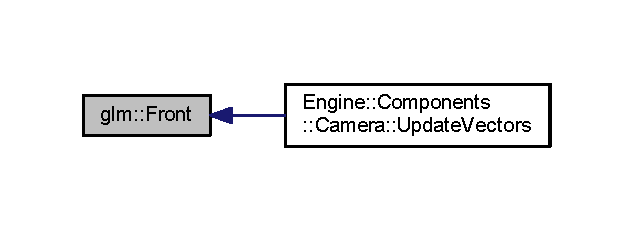
\includegraphics[width=304pt]{namespaceglm_a95e780de06846d0eee634d15187b87ab_icgraph}
\end{center}
\end{figure}
\mbox{\Hypertarget{namespaceglm_a23fef243f5fe738c94f80aad5bf5087d}\label{namespaceglm_a23fef243f5fe738c94f80aad5bf5087d}} 
\index{glm@{glm}!Left@{Left}}
\index{Left@{Left}!glm@{glm}}
\subsubsection{\texorpdfstring{Left()}{Left()}}
{\footnotesize\ttfamily vec3 glm\+::\+Left (\begin{DoxyParamCaption}\item[{-\/}]{1,  }\item[{0}]{,  }\item[{0}]{ }\end{DoxyParamCaption})}

\mbox{\Hypertarget{namespaceglm_a8726baea7dc7bb32e57d33b0333d1def}\label{namespaceglm_a8726baea7dc7bb32e57d33b0333d1def}} 
\index{glm@{glm}!Right@{Right}}
\index{Right@{Right}!glm@{glm}}
\subsubsection{\texorpdfstring{Right()}{Right()}}
{\footnotesize\ttfamily vec3 glm\+::\+Right (\begin{DoxyParamCaption}\item[{1}]{,  }\item[{0}]{,  }\item[{0}]{ }\end{DoxyParamCaption})}



Referenced by Engine\+::\+Components\+::\+Camera\+::\+Update\+Vectors().

Here is the caller graph for this function\+:
\nopagebreak
\begin{figure}[H]
\begin{center}
\leavevmode
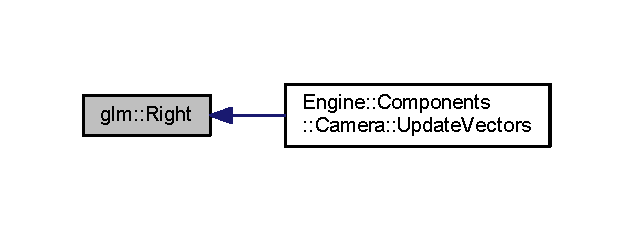
\includegraphics[width=304pt]{namespaceglm_a8726baea7dc7bb32e57d33b0333d1def_icgraph}
\end{center}
\end{figure}
\mbox{\Hypertarget{namespaceglm_a885c1f58e3aeeb85a2bfacd2c741e8d3}\label{namespaceglm_a885c1f58e3aeeb85a2bfacd2c741e8d3}} 
\index{glm@{glm}!rotate\+Around@{rotate\+Around}}
\index{rotate\+Around@{rotate\+Around}!glm@{glm}}
\subsubsection{\texorpdfstring{rotate\+Around()}{rotateAround()}}
{\footnotesize\ttfamily vec2 glm\+::rotate\+Around (\begin{DoxyParamCaption}\item[{vec2}]{center,  }\item[{vec2}]{point,  }\item[{float}]{angle }\end{DoxyParamCaption})\hspace{0.3cm}{\ttfamily [inline]}}



Definition at line 32 of file gml\+Extensions.\+h.


\begin{DoxyCode}
32                                                                    \{
33 
34         \textcolor{keywordflow}{return} vec2(cos(angle) * (point.x - center.x) - sin(angle) * (point.y - center.y) + center.x,
35                     sin(angle) * (point.x - center.x) + cos(angle) * (point.y - center.y) + center.y);
36     \}
\end{DoxyCode}
\mbox{\Hypertarget{namespaceglm_a877b2ed5ef3e542d953a0768f9494f2b}\label{namespaceglm_a877b2ed5ef3e542d953a0768f9494f2b}} 
\index{glm@{glm}!simplify@{simplify}}
\index{simplify@{simplify}!glm@{glm}}
\subsubsection{\texorpdfstring{simplify()}{simplify()}\hspace{0.1cm}{\footnotesize\ttfamily [1/3]}}
{\footnotesize\ttfamily float glm\+::simplify (\begin{DoxyParamCaption}\item[{float}]{vector,  }\item[{float}]{value = {\ttfamily 1.f} }\end{DoxyParamCaption})\hspace{0.3cm}{\ttfamily [inline]}}



Definition at line 7 of file gml\+Extensions.\+h.



Referenced by simplify().


\begin{DoxyCode}
8     \{
9         \textcolor{keywordflow}{if} (vector > 0)
10             \textcolor{keywordflow}{return} value;
11         \textcolor{keywordflow}{if} (vector < 0)
12             \textcolor{keywordflow}{return} -value;
13         \textcolor{keywordflow}{return} 0.f;
14     \}
\end{DoxyCode}
Here is the caller graph for this function\+:
\nopagebreak
\begin{figure}[H]
\begin{center}
\leavevmode
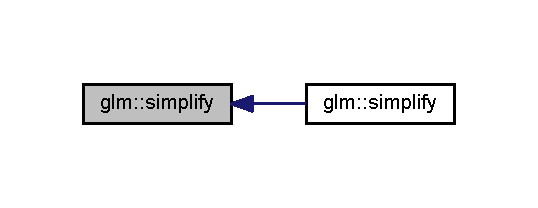
\includegraphics[width=258pt]{namespaceglm_a877b2ed5ef3e542d953a0768f9494f2b_icgraph}
\end{center}
\end{figure}
\mbox{\Hypertarget{namespaceglm_a1b1223920ce15b9bc024049ebc24ac25}\label{namespaceglm_a1b1223920ce15b9bc024049ebc24ac25}} 
\index{glm@{glm}!simplify@{simplify}}
\index{simplify@{simplify}!glm@{glm}}
\subsubsection{\texorpdfstring{simplify()}{simplify()}\hspace{0.1cm}{\footnotesize\ttfamily [2/3]}}
{\footnotesize\ttfamily vec3 glm\+::simplify (\begin{DoxyParamCaption}\item[{glm\+::vec3}]{vector,  }\item[{float}]{value = {\ttfamily 1.f} }\end{DoxyParamCaption})\hspace{0.3cm}{\ttfamily [inline]}}



Definition at line 16 of file gml\+Extensions.\+h.



References simplify().


\begin{DoxyCode}
17     \{
18         \textcolor{keyword}{auto} v = vector;
19         v.x = \mbox{\hyperlink{namespaceglm_a091978f9c1c830d7388c42251c59dad4}{simplify}}(v.x,value);
20         v.y = \mbox{\hyperlink{namespaceglm_a091978f9c1c830d7388c42251c59dad4}{simplify}}(v.y, value);
21         v.z = \mbox{\hyperlink{namespaceglm_a091978f9c1c830d7388c42251c59dad4}{simplify}}(v.z, value);
22         \textcolor{keywordflow}{return} v;
23     \}
\end{DoxyCode}
Here is the call graph for this function\+:
\nopagebreak
\begin{figure}[H]
\begin{center}
\leavevmode
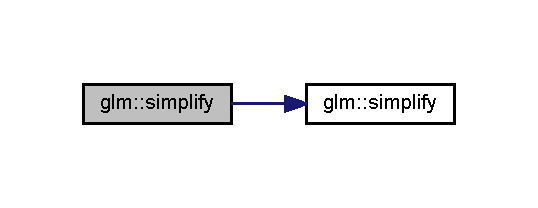
\includegraphics[width=258pt]{namespaceglm_a1b1223920ce15b9bc024049ebc24ac25_cgraph}
\end{center}
\end{figure}
\mbox{\Hypertarget{namespaceglm_a091978f9c1c830d7388c42251c59dad4}\label{namespaceglm_a091978f9c1c830d7388c42251c59dad4}} 
\index{glm@{glm}!simplify@{simplify}}
\index{simplify@{simplify}!glm@{glm}}
\subsubsection{\texorpdfstring{simplify()}{simplify()}\hspace{0.1cm}{\footnotesize\ttfamily [3/3]}}
{\footnotesize\ttfamily vec2 glm\+::simplify (\begin{DoxyParamCaption}\item[{glm\+::vec2}]{vector,  }\item[{float}]{value = {\ttfamily 1.f} }\end{DoxyParamCaption})\hspace{0.3cm}{\ttfamily [inline]}}



Definition at line 24 of file gml\+Extensions.\+h.



References simplify().


\begin{DoxyCode}
25     \{
26         \textcolor{keyword}{auto} v = vector;
27         v.x = \mbox{\hyperlink{namespaceglm_a091978f9c1c830d7388c42251c59dad4}{simplify}}(v.x, value);
28         v.y = \mbox{\hyperlink{namespaceglm_a091978f9c1c830d7388c42251c59dad4}{simplify}}(v.y, value);
29         \textcolor{keywordflow}{return} v;
30     \}
\end{DoxyCode}
Here is the call graph for this function\+:
\nopagebreak
\begin{figure}[H]
\begin{center}
\leavevmode
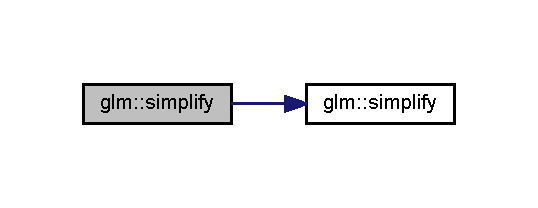
\includegraphics[width=258pt]{namespaceglm_a091978f9c1c830d7388c42251c59dad4_cgraph}
\end{center}
\end{figure}
\mbox{\Hypertarget{namespaceglm_a35741e27838ab920dff5fbaba619829e}\label{namespaceglm_a35741e27838ab920dff5fbaba619829e}} 
\index{glm@{glm}!Up@{Up}}
\index{Up@{Up}!glm@{glm}}
\subsubsection{\texorpdfstring{Up()}{Up()}}
{\footnotesize\ttfamily vec3 glm\+::\+Up (\begin{DoxyParamCaption}\item[{0}]{,  }\item[{1}]{,  }\item[{0}]{ }\end{DoxyParamCaption})}



Referenced by Engine\+::\+Components\+::\+Camera\+::\+Get(), Engine\+::\+Components\+::\+Camera\+::\+Set\+Up(), and Engine\+::\+Components\+::\+Camera\+::\+Update\+Vectors().

Here is the caller graph for this function\+:
\nopagebreak
\begin{figure}[H]
\begin{center}
\leavevmode
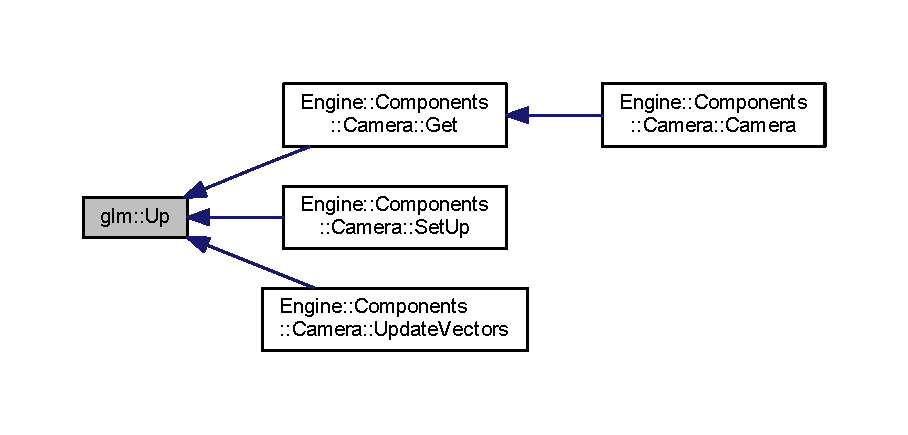
\includegraphics[width=350pt]{namespaceglm_a35741e27838ab920dff5fbaba619829e_icgraph}
\end{center}
\end{figure}

\chapter{Class Documentation}
\hypertarget{classApplication_1_1Application}{}\section{Application\+:\+:Application Class Reference}
\label{classApplication_1_1Application}\index{Application\+::\+Application@{Application\+::\+Application}}


{\ttfamily \#include $<$Application.\+h$>$}



Collaboration diagram for Application\+:\+:Application\+:
\nopagebreak
\begin{figure}[H]
\begin{center}
\leavevmode
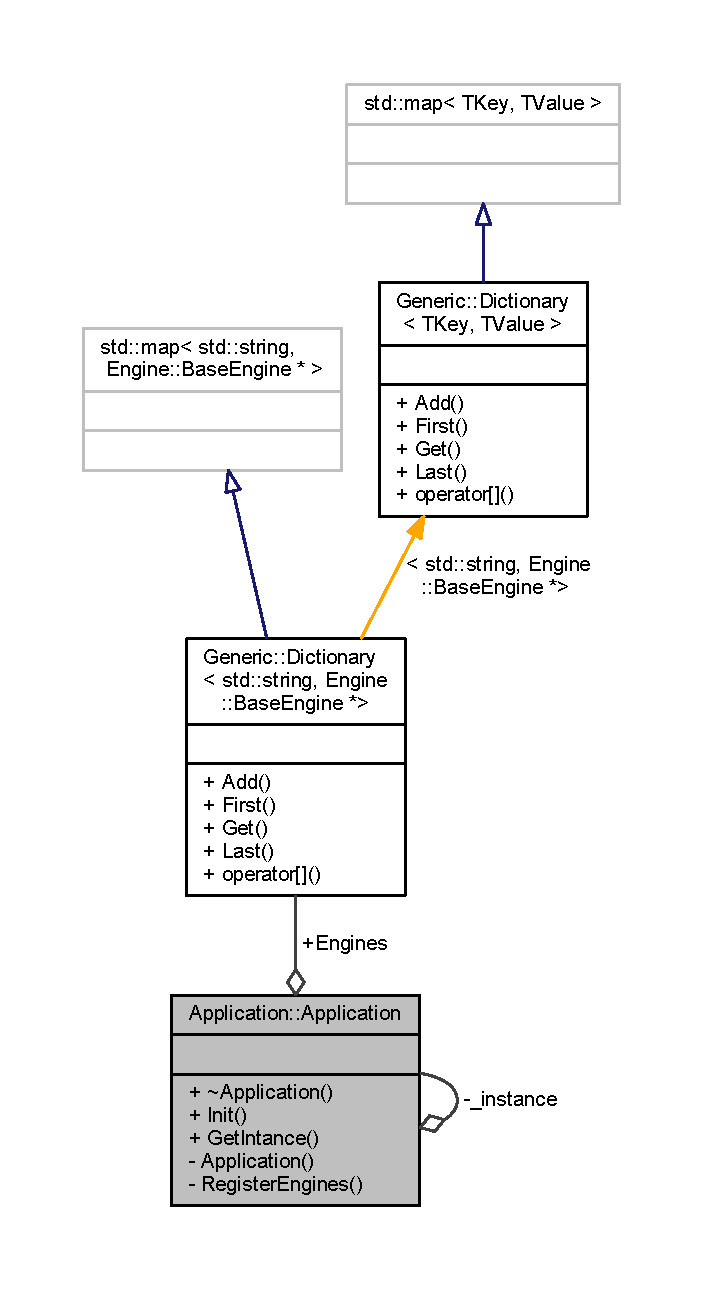
\includegraphics[height=550pt]{classApplication_1_1Application__coll__graph}
\end{center}
\end{figure}
\subsection*{Public Member Functions}
\begin{DoxyCompactItemize}
\item 
\mbox{\hyperlink{classApplication_1_1Application_aeef3ff221435f74e41115640239e6f34}{$\sim$\+Application}} ()
\item 
\mbox{\hyperlink{classApplication_1_1Application}{Application}} $\ast$ \mbox{\hyperlink{classApplication_1_1Application_a478f6946c4bf5361281681f2b58385c3}{Init}} ()
\end{DoxyCompactItemize}
\subsection*{Static Public Member Functions}
\begin{DoxyCompactItemize}
\item 
static \mbox{\hyperlink{classApplication_1_1Application}{Application}} $\ast$ \mbox{\hyperlink{classApplication_1_1Application_ada268208f57ef136e006bb62fb30ffec}{Get\+Intance}} ()
\end{DoxyCompactItemize}
\subsection*{Public Attributes}
\begin{DoxyCompactItemize}
\item 
\mbox{\hyperlink{classGeneric_1_1Dictionary}{Generic\+::\+Dictionary}}$<$ std\+::string, \mbox{\hyperlink{classEngine_1_1BaseEngine}{Engine\+::\+Base\+Engine}} $\ast$ $>$ $\ast$ \mbox{\hyperlink{classApplication_1_1Application_a4f2808bddfc3f8fb2ed3a3fe0d4659ff}{Engines}}
\end{DoxyCompactItemize}
\subsection*{Private Member Functions}
\begin{DoxyCompactItemize}
\item 
\mbox{\hyperlink{classApplication_1_1Application_aa27a092cca399b3ccee7419a7cda4563}{Application}} ()
\item 
void \mbox{\hyperlink{classApplication_1_1Application_a877f88238e07698fb9fcc0b71e9f15e7}{Register\+Engines}} ()
\end{DoxyCompactItemize}
\subsection*{Static Private Attributes}
\begin{DoxyCompactItemize}
\item 
static \mbox{\hyperlink{classApplication_1_1Application}{Application}} \mbox{\hyperlink{classApplication_1_1Application_abd6690c71308921648b3b4da20d604d9}{\+\_\+instance}}
\end{DoxyCompactItemize}


\subsection{Detailed Description}


Definition at line 8 of file Application.\+h.



\subsection{Constructor \& Destructor Documentation}
\mbox{\Hypertarget{classApplication_1_1Application_aeef3ff221435f74e41115640239e6f34}\label{classApplication_1_1Application_aeef3ff221435f74e41115640239e6f34}} 
\index{Application\+::\+Application@{Application\+::\+Application}!````~Application@{$\sim$\+Application}}
\index{````~Application@{$\sim$\+Application}!Application\+::\+Application@{Application\+::\+Application}}
\subsubsection{\texorpdfstring{$\sim$\+Application()}{~Application()}}
{\footnotesize\ttfamily Application\+::\+Application\+::$\sim$\+Application (\begin{DoxyParamCaption}{ }\end{DoxyParamCaption})}



Definition at line 13 of file Application.\+cpp.


\begin{DoxyCode}
14 \{
15     \mbox{\hyperlink{classApplication_1_1Application_a4f2808bddfc3f8fb2ed3a3fe0d4659ff}{Engines}}->clear();
16     \textcolor{keyword}{delete} \mbox{\hyperlink{classApplication_1_1Application_a4f2808bddfc3f8fb2ed3a3fe0d4659ff}{Engines}};
17 \}
\end{DoxyCode}
\mbox{\Hypertarget{classApplication_1_1Application_aa27a092cca399b3ccee7419a7cda4563}\label{classApplication_1_1Application_aa27a092cca399b3ccee7419a7cda4563}} 
\index{Application\+::\+Application@{Application\+::\+Application}!Application@{Application}}
\index{Application@{Application}!Application\+::\+Application@{Application\+::\+Application}}
\subsubsection{\texorpdfstring{Application()}{Application()}}
{\footnotesize\ttfamily Application\+::\+Application\+::\+Application (\begin{DoxyParamCaption}{ }\end{DoxyParamCaption})\hspace{0.3cm}{\ttfamily [private]}}



Definition at line 8 of file Application.\+cpp.


\begin{DoxyCode}
9 \{
10     \mbox{\hyperlink{classApplication_1_1Application_a4f2808bddfc3f8fb2ed3a3fe0d4659ff}{Engines}} = \textcolor{keyword}{new} \mbox{\hyperlink{classGeneric_1_1Dictionary}{Generic::Dictionary<std::string, Engine::BaseEngine*>}}
      ();
11 \}
\end{DoxyCode}


\subsection{Member Function Documentation}
\mbox{\Hypertarget{classApplication_1_1Application_ada268208f57ef136e006bb62fb30ffec}\label{classApplication_1_1Application_ada268208f57ef136e006bb62fb30ffec}} 
\index{Application\+::\+Application@{Application\+::\+Application}!Get\+Intance@{Get\+Intance}}
\index{Get\+Intance@{Get\+Intance}!Application\+::\+Application@{Application\+::\+Application}}
\subsubsection{\texorpdfstring{Get\+Intance()}{GetIntance()}}
{\footnotesize\ttfamily \mbox{\hyperlink{classApplication_1_1Application}{Application\+::\+Application}} $\ast$ Application\+::\+Application\+::\+Get\+Intance (\begin{DoxyParamCaption}{ }\end{DoxyParamCaption})\hspace{0.3cm}{\ttfamily [static]}}



Definition at line 19 of file Application.\+cpp.



Referenced by main().


\begin{DoxyCode}
20 \{
21     \textcolor{keyword}{static} \mbox{\hyperlink{namespaceApplication}{Application}} instance;
22     \textcolor{keywordflow}{return} &instance;
23 \}
\end{DoxyCode}
Here is the caller graph for this function\+:
\nopagebreak
\begin{figure}[H]
\begin{center}
\leavevmode
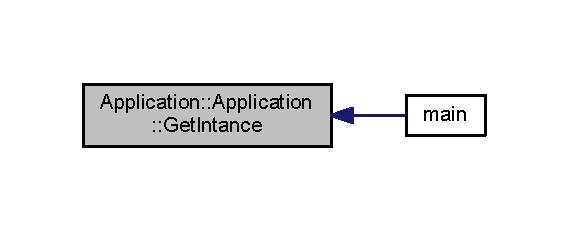
\includegraphics[width=273pt]{classApplication_1_1Application_ada268208f57ef136e006bb62fb30ffec_icgraph}
\end{center}
\end{figure}
\mbox{\Hypertarget{classApplication_1_1Application_a478f6946c4bf5361281681f2b58385c3}\label{classApplication_1_1Application_a478f6946c4bf5361281681f2b58385c3}} 
\index{Application\+::\+Application@{Application\+::\+Application}!Init@{Init}}
\index{Init@{Init}!Application\+::\+Application@{Application\+::\+Application}}
\subsubsection{\texorpdfstring{Init()}{Init()}}
{\footnotesize\ttfamily \mbox{\hyperlink{classApplication_1_1Application}{Application\+::\+Application}} $\ast$ Application\+::\+Application\+::\+Init (\begin{DoxyParamCaption}{ }\end{DoxyParamCaption})}



Definition at line 25 of file Application.\+cpp.



Referenced by main().


\begin{DoxyCode}
26 \{
27     \mbox{\hyperlink{classApplication_1_1Application_a877f88238e07698fb9fcc0b71e9f15e7}{RegisterEngines}}();
28     \textcolor{keywordflow}{return} \textcolor{keyword}{this};
29 \}
\end{DoxyCode}
Here is the caller graph for this function\+:
\nopagebreak
\begin{figure}[H]
\begin{center}
\leavevmode
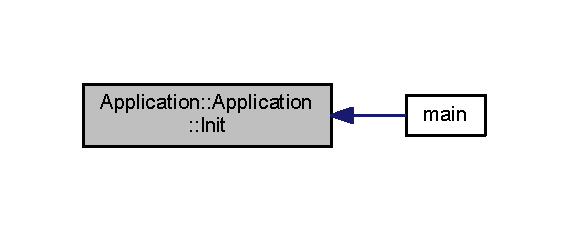
\includegraphics[width=273pt]{classApplication_1_1Application_a478f6946c4bf5361281681f2b58385c3_icgraph}
\end{center}
\end{figure}
\mbox{\Hypertarget{classApplication_1_1Application_a877f88238e07698fb9fcc0b71e9f15e7}\label{classApplication_1_1Application_a877f88238e07698fb9fcc0b71e9f15e7}} 
\index{Application\+::\+Application@{Application\+::\+Application}!Register\+Engines@{Register\+Engines}}
\index{Register\+Engines@{Register\+Engines}!Application\+::\+Application@{Application\+::\+Application}}
\subsubsection{\texorpdfstring{Register\+Engines()}{RegisterEngines()}}
{\footnotesize\ttfamily void Application\+::\+Application\+::\+Register\+Engines (\begin{DoxyParamCaption}{ }\end{DoxyParamCaption})\hspace{0.3cm}{\ttfamily [private]}}



Definition at line 7 of file Engine\+Registry.\+cpp.


\begin{DoxyCode}
8 \{
9     \mbox{\hyperlink{classApplication_1_1Application_a4f2808bddfc3f8fb2ed3a3fe0d4659ff}{Engines}}->
10          Add(\textcolor{stringliteral}{"basic"}, \textcolor{keyword}{new} Engines::BasicEngine())
11         .\mbox{\hyperlink{classGeneric_1_1Dictionary_ae7cb006f801b21c172e8fbac8794fa99}{Add}}(\textcolor{stringliteral}{"camera"}, \textcolor{keyword}{new} Engines::CameraEngine())
12         .\mbox{\hyperlink{classGeneric_1_1Dictionary_ae7cb006f801b21c172e8fbac8794fa99}{Add}}(\textcolor{stringliteral}{"light"}, \textcolor{keyword}{new} Engines::LightEngine())
13     ;
14 \}
\end{DoxyCode}


\subsection{Member Data Documentation}
\mbox{\Hypertarget{classApplication_1_1Application_abd6690c71308921648b3b4da20d604d9}\label{classApplication_1_1Application_abd6690c71308921648b3b4da20d604d9}} 
\index{Application\+::\+Application@{Application\+::\+Application}!\+\_\+instance@{\+\_\+instance}}
\index{\+\_\+instance@{\+\_\+instance}!Application\+::\+Application@{Application\+::\+Application}}
\subsubsection{\texorpdfstring{\+\_\+instance}{\_instance}}
{\footnotesize\ttfamily \mbox{\hyperlink{classApplication_1_1Application}{Application}} Application\+::\+Application\+::\+\_\+instance\hspace{0.3cm}{\ttfamily [static]}, {\ttfamily [private]}}



Definition at line 17 of file Application.\+h.

\mbox{\Hypertarget{classApplication_1_1Application_a4f2808bddfc3f8fb2ed3a3fe0d4659ff}\label{classApplication_1_1Application_a4f2808bddfc3f8fb2ed3a3fe0d4659ff}} 
\index{Application\+::\+Application@{Application\+::\+Application}!Engines@{Engines}}
\index{Engines@{Engines}!Application\+::\+Application@{Application\+::\+Application}}
\subsubsection{\texorpdfstring{Engines}{Engines}}
{\footnotesize\ttfamily \mbox{\hyperlink{classGeneric_1_1Dictionary}{Generic\+::\+Dictionary}}$<$std\+::string, \mbox{\hyperlink{classEngine_1_1BaseEngine}{Engine\+::\+Base\+Engine}}$\ast$$>$$\ast$ Application\+::\+Application\+::\+Engines}



Definition at line 14 of file Application.\+h.



Referenced by main().



The documentation for this class was generated from the following files\+:\begin{DoxyCompactItemize}
\item 
Z\+P\+G/\mbox{\hyperlink{Application_8h}{Application.\+h}}\item 
Z\+P\+G/\mbox{\hyperlink{Application_8cpp}{Application.\+cpp}}\item 
Z\+P\+G/\mbox{\hyperlink{EngineRegistry_8cpp}{Engine\+Registry.\+cpp}}\end{DoxyCompactItemize}

\hypertarget{classApplication_1_1Engines_1_1BasicEngine}{}\section{Application\+:\+:Engines\+:\+:Basic\+Engine Class Reference}
\label{classApplication_1_1Engines_1_1BasicEngine}\index{Application\+::\+Engines\+::\+Basic\+Engine@{Application\+::\+Engines\+::\+Basic\+Engine}}


{\ttfamily \#include $<$Basic\+Engine.\+h$>$}



Inheritance diagram for Application\+:\+:Engines\+:\+:Basic\+Engine\+:
\nopagebreak
\begin{figure}[H]
\begin{center}
\leavevmode
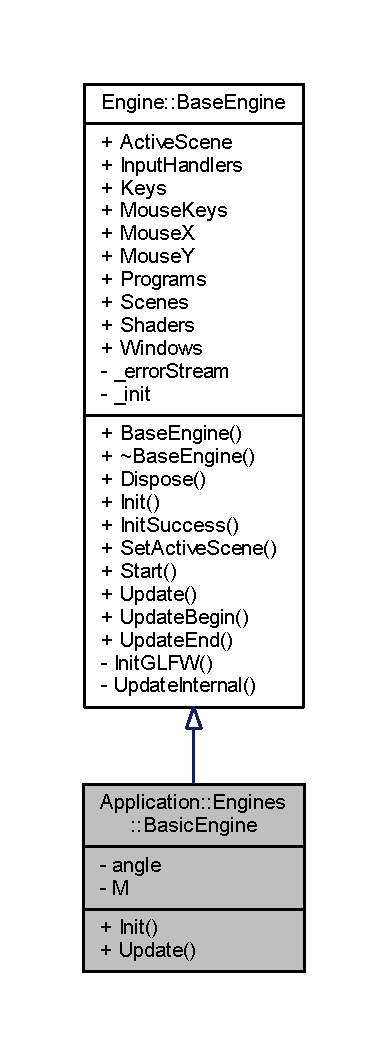
\includegraphics[width=186pt]{classApplication_1_1Engines_1_1BasicEngine__inherit__graph}
\end{center}
\end{figure}


Collaboration diagram for Application\+:\+:Engines\+:\+:Basic\+Engine\+:
\nopagebreak
\begin{figure}[H]
\begin{center}
\leavevmode
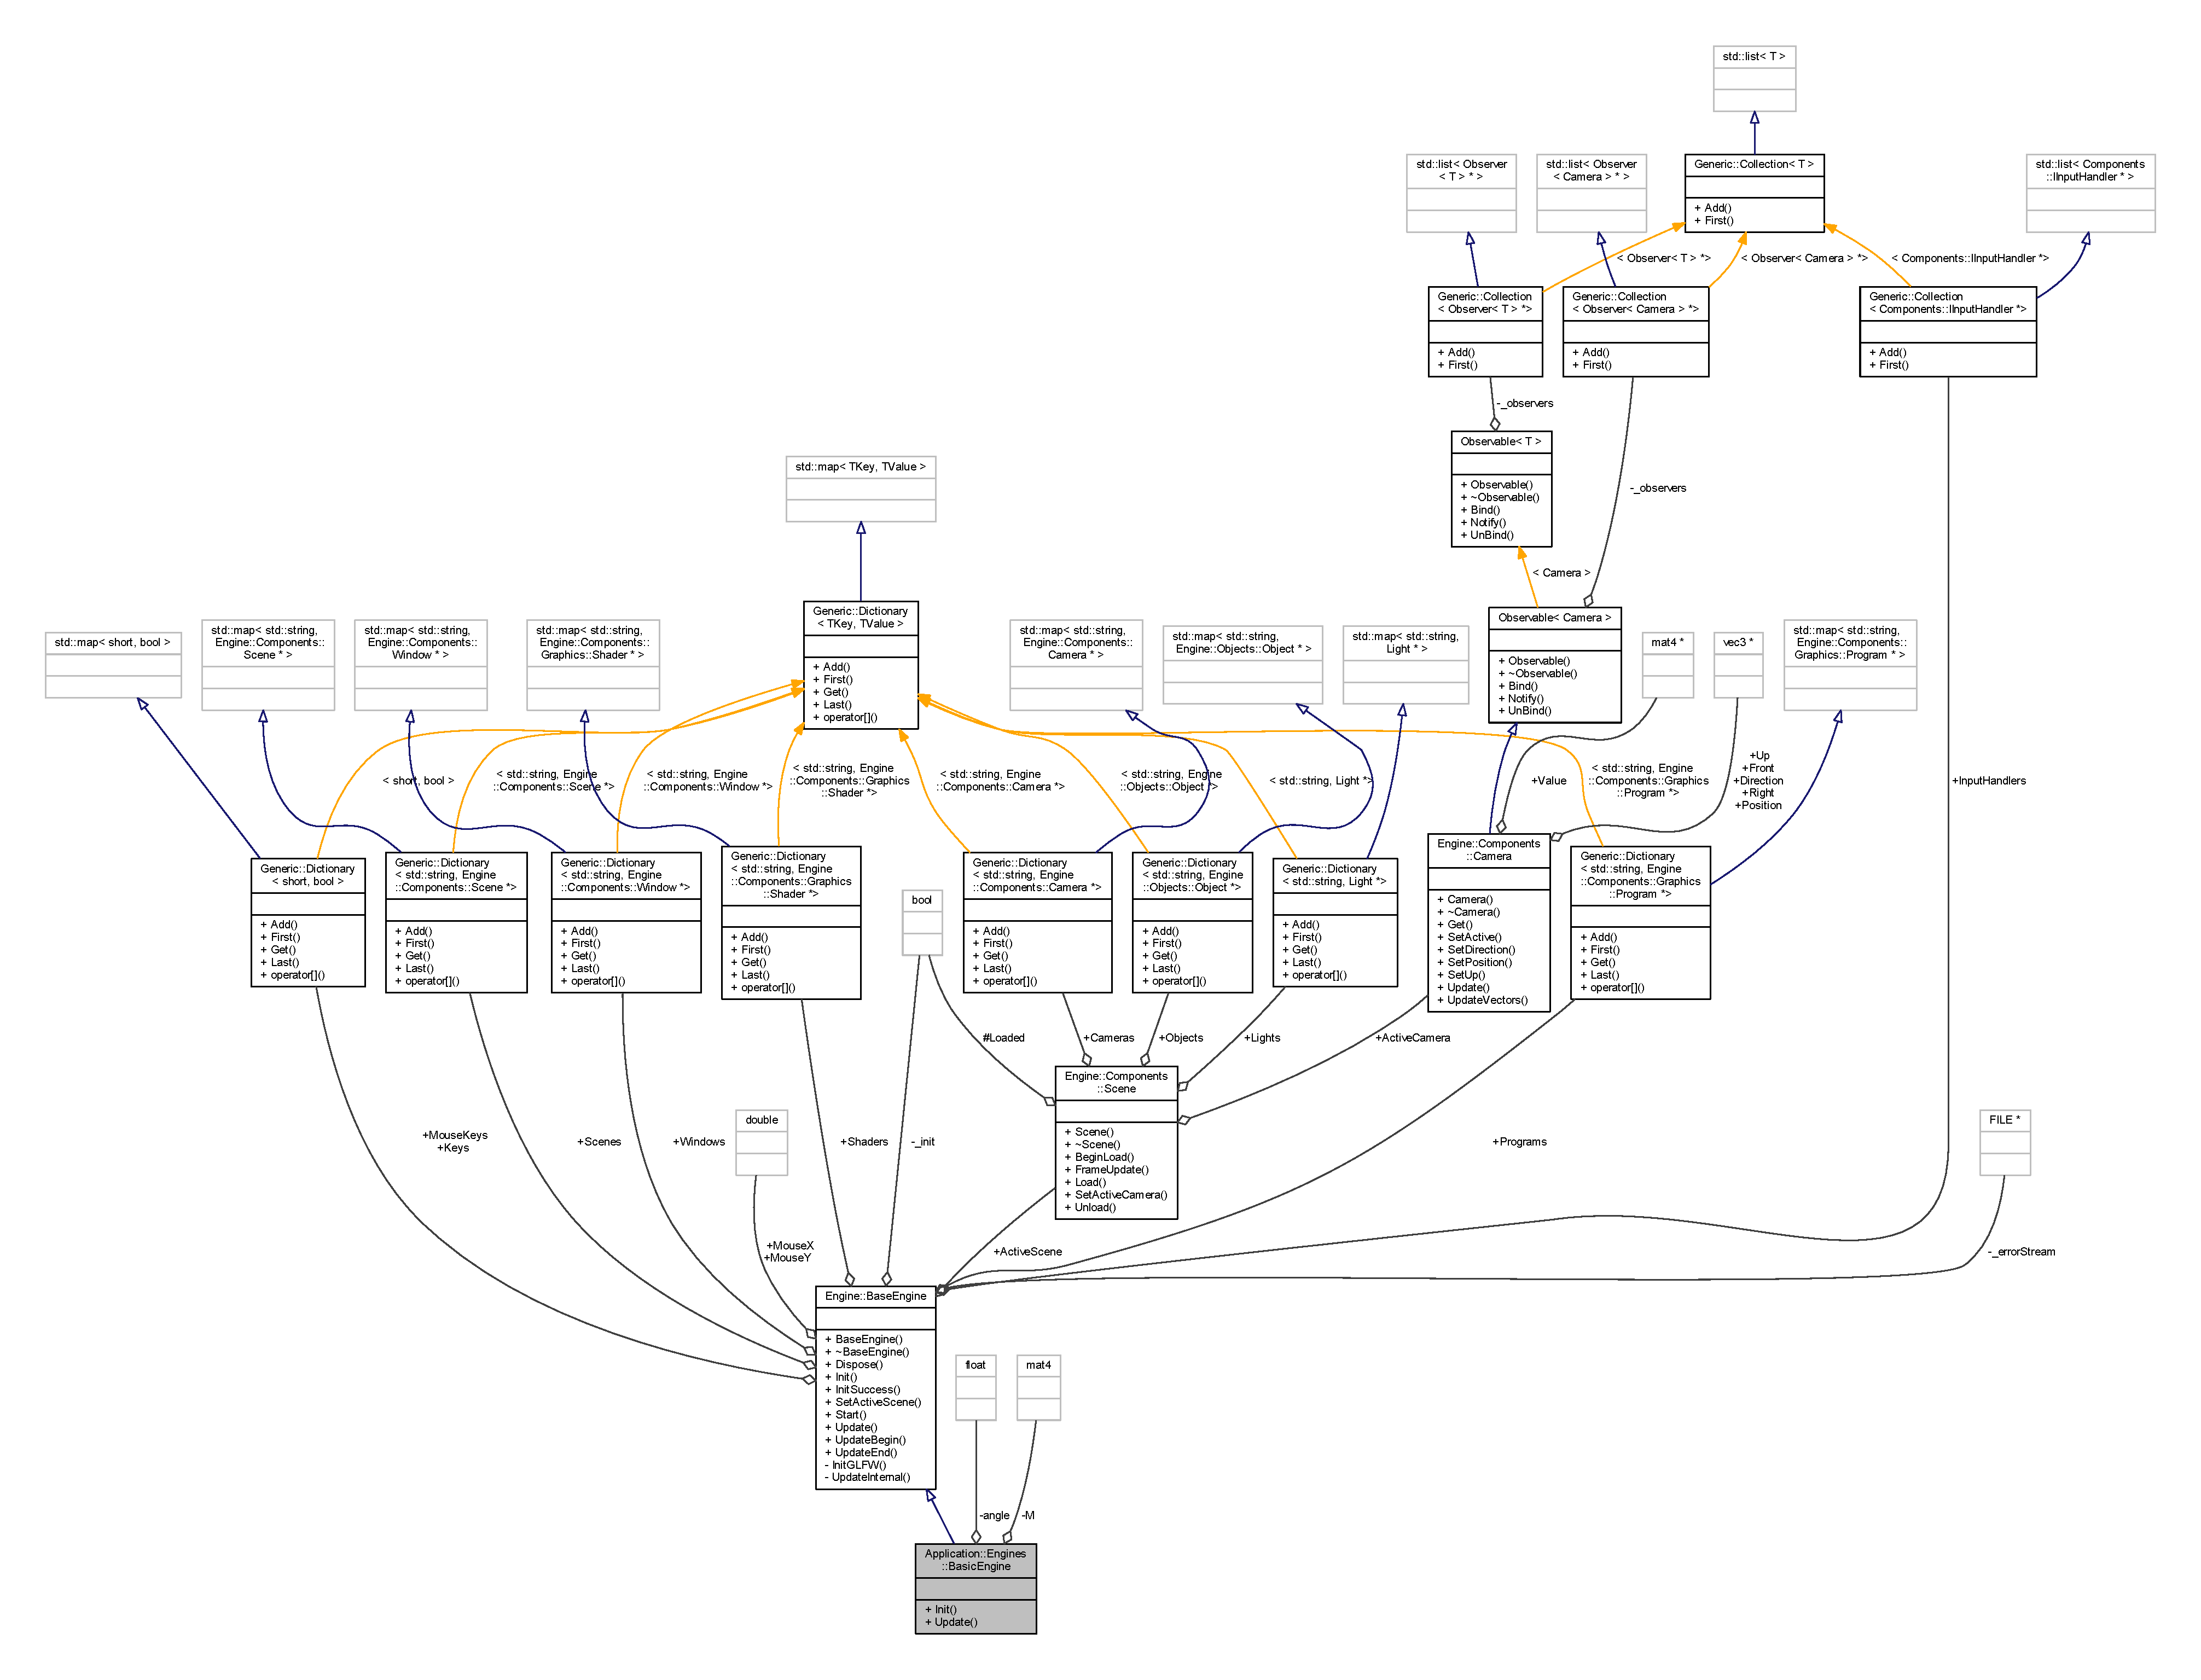
\includegraphics[width=350pt]{classApplication_1_1Engines_1_1BasicEngine__coll__graph}
\end{center}
\end{figure}
\subsection*{Public Member Functions}
\begin{DoxyCompactItemize}
\item 
\mbox{\hyperlink{classEngine_1_1BaseEngine_ad838c97afe1790cb35527f0b58e81e6b}{Base\+Engine}} $\ast$ \mbox{\hyperlink{classEngine_1_1BaseEngine_acd5cd5d2189d24e038b23477b7dce405}{Dispose}} ()
\item 
\mbox{\hyperlink{classApplication_1_1Engines_1_1BasicEngine}{Basic\+Engine}} $\ast$ \mbox{\hyperlink{classApplication_1_1Engines_1_1BasicEngine_afbdc9f559d1776371f90da00b61ba6ab}{Init}} (std\+::\+F\+I\+LE $\ast$error\+Stream=stderr) override
\item 
bool \mbox{\hyperlink{classEngine_1_1BaseEngine_a7a1c9b833049b3eb61194cab113dfe89}{Init\+Success}} ()
\item 
virtual void \mbox{\hyperlink{classEngine_1_1BaseEngine_afc82c6a00d5a9d4714740fc5eab5db86}{Set\+Active\+Scene}} (Components\+::\+Scene $\ast$scene=nullptr)
\item 
virtual void \mbox{\hyperlink{classEngine_1_1BaseEngine_a525fdc7a1da7eecb514ad5763f06be79}{Start}} ()
\item 
void \mbox{\hyperlink{classApplication_1_1Engines_1_1BasicEngine_ad628d9878f5008dd7f7f7743a75d5f17}{Update}} (\+::\mbox{\hyperlink{classEngine_1_1Components_1_1Window}{Engine\+::\+Components\+::\+Window}} $\ast$window) override
\item 
virtual void \mbox{\hyperlink{classEngine_1_1BaseEngine_a01c23c2073f08939a660f3b7a866852c}{Update}} (Components\+::\+Window $\ast$window)
\item 
virtual void \mbox{\hyperlink{classEngine_1_1BaseEngine_aace6be2a42d12b64fbd35f1acdb08408}{Update\+Begin}} (Components\+::\+Window $\ast$window)
\item 
virtual void \mbox{\hyperlink{classEngine_1_1BaseEngine_a7c07c98e583df042a0eb01e0ddec85a1}{Update\+End}} (Components\+::\+Window $\ast$window)
\end{DoxyCompactItemize}
\subsection*{Public Attributes}
\begin{DoxyCompactItemize}
\item 
Components\+::\+Scene $\ast$ \mbox{\hyperlink{classEngine_1_1BaseEngine_adb3dbc839da9d821e08b18d8a221698d}{Active\+Scene}}
\item 
\mbox{\hyperlink{classGeneric_1_1Collection}{Generic\+::\+Collection}}$<$ Components\+::\+I\+Input\+Handler $\ast$ $>$ $\ast$ \mbox{\hyperlink{classEngine_1_1BaseEngine_a134fa082c5a64d62b76ddf926647e7cc}{Input\+Handlers}}
\item 
\mbox{\hyperlink{classGeneric_1_1Dictionary}{Generic\+::\+Dictionary}}$<$ short, bool $>$ \mbox{\hyperlink{classEngine_1_1BaseEngine_a65321a97e83f0a6ee90df3efac2d3307}{Keys}}
\item 
\mbox{\hyperlink{classGeneric_1_1Dictionary}{Generic\+::\+Dictionary}}$<$ short, bool $>$ \mbox{\hyperlink{classEngine_1_1BaseEngine_a3ee2bdddb66d45b8c808ffd937ba9c50}{Mouse\+Keys}}
\item 
double \mbox{\hyperlink{classEngine_1_1BaseEngine_a5fe085152ebe93346900407f6b41a034}{MouseX}}
\item 
double \mbox{\hyperlink{classEngine_1_1BaseEngine_a143c9c32dbbdc70bf1546ffe275bf384}{MouseY}}
\item 
\mbox{\hyperlink{classGeneric_1_1Dictionary}{Generic\+::\+Dictionary}}$<$ std\+::string, Components\+::\+Graphics\+::\+Program $\ast$ $>$ $\ast$ \mbox{\hyperlink{classEngine_1_1BaseEngine_ae0f86360ea3a384caefe443dd8f88601}{Programs}}
\item 
\mbox{\hyperlink{classGeneric_1_1Dictionary}{Generic\+::\+Dictionary}}$<$ std\+::string, Components\+::\+Scene $\ast$ $>$ $\ast$ \mbox{\hyperlink{classEngine_1_1BaseEngine_afd02af3c2fbe9bb734db014dec06585a}{Scenes}}
\item 
\mbox{\hyperlink{classGeneric_1_1Dictionary}{Generic\+::\+Dictionary}}$<$ std\+::string, Components\+::\+Graphics\+::\+Shader $\ast$ $>$ $\ast$ \mbox{\hyperlink{classEngine_1_1BaseEngine_a2582dee3f73da82bb422b43317b85e3b}{Shaders}}
\item 
\mbox{\hyperlink{classGeneric_1_1Dictionary}{Generic\+::\+Dictionary}}$<$ std\+::string, Components\+::\+Window $\ast$ $>$ $\ast$ \mbox{\hyperlink{classEngine_1_1BaseEngine_a4a1a4c4dae052e66ecc4f326eeed4d33}{Windows}}
\end{DoxyCompactItemize}
\subsection*{Private Attributes}
\begin{DoxyCompactItemize}
\item 
float \mbox{\hyperlink{classApplication_1_1Engines_1_1BasicEngine_aad99e45bc67ec33b4fc26b38b9c8a31e}{angle}}
\item 
glm\+::mat4 \mbox{\hyperlink{classApplication_1_1Engines_1_1BasicEngine_a645ebb7fc6a7eb2961a5c15986a0c246}{M}}
\end{DoxyCompactItemize}


\subsection{Detailed Description}


Definition at line 8 of file Basic\+Engine.\+h.



\subsection{Member Function Documentation}
\mbox{\Hypertarget{classEngine_1_1BaseEngine_acd5cd5d2189d24e038b23477b7dce405}\label{classEngine_1_1BaseEngine_acd5cd5d2189d24e038b23477b7dce405}} 
\index{Application\+::\+Engines\+::\+Basic\+Engine@{Application\+::\+Engines\+::\+Basic\+Engine}!Dispose@{Dispose}}
\index{Dispose@{Dispose}!Application\+::\+Engines\+::\+Basic\+Engine@{Application\+::\+Engines\+::\+Basic\+Engine}}
\subsubsection{\texorpdfstring{Dispose()}{Dispose()}}
{\footnotesize\ttfamily \mbox{\hyperlink{classEngine_1_1BaseEngine}{Engine\+::\+Base\+Engine}} $\ast$ Engine\+::\+Base\+Engine\+::\+Dispose (\begin{DoxyParamCaption}{ }\end{DoxyParamCaption})\hspace{0.3cm}{\ttfamily [inherited]}}



Definition at line 51 of file Base\+Engine.\+cpp.


\begin{DoxyCode}
52 \{
53     glfwTerminate();
54     \textcolor{keywordflow}{return} \textcolor{keyword}{this};
55 \}
\end{DoxyCode}
\mbox{\Hypertarget{classApplication_1_1Engines_1_1BasicEngine_afbdc9f559d1776371f90da00b61ba6ab}\label{classApplication_1_1Engines_1_1BasicEngine_afbdc9f559d1776371f90da00b61ba6ab}} 
\index{Application\+::\+Engines\+::\+Basic\+Engine@{Application\+::\+Engines\+::\+Basic\+Engine}!Init@{Init}}
\index{Init@{Init}!Application\+::\+Engines\+::\+Basic\+Engine@{Application\+::\+Engines\+::\+Basic\+Engine}}
\subsubsection{\texorpdfstring{Init()}{Init()}}
{\footnotesize\ttfamily \mbox{\hyperlink{classApplication_1_1Engines_1_1BasicEngine}{Application\+::\+Engines\+::\+Basic\+Engine}} $\ast$ Application\+::\+Engines\+::\+Basic\+Engine\+::\+Init (\begin{DoxyParamCaption}\item[{std\+::\+F\+I\+LE $\ast$}]{error\+Stream = {\ttfamily stderr} }\end{DoxyParamCaption})\hspace{0.3cm}{\ttfamily [override]}, {\ttfamily [virtual]}}



Reimplemented from \mbox{\hyperlink{classEngine_1_1BaseEngine_ad9c141fe48c8c91e14e77ed5fcb90196}{Engine\+::\+Base\+Engine}}.



Definition at line 8 of file Basic\+Engine.\+cpp.



References angle, fragment\+\_\+shader, M, Engine\+::\+Base\+Engine\+::\+Programs, Engine\+::\+Base\+Engine\+::\+Scenes, Engine\+::\+Base\+Engine\+::\+Set\+Active\+Scene(), Engine\+::\+Base\+Engine\+::\+Shaders, Assets\+::\+Shaders\+Fragment, Assets\+::\+Shaders\+Vertex, vertex\+\_\+shader, and Engine\+::\+Base\+Engine\+::\+Windows.


\begin{DoxyCode}
9 \{
10     BaseEngine::Init(errorStream);
11 
12     \textcolor{keyword}{const} \textcolor{keywordtype}{char}* \mbox{\hyperlink{ZPGEngine_8cpp_afc33b8912f9f93d1d2544df04ad4a81a}{vertex\_shader}} =
13         \textcolor{stringliteral}{"#version 330\(\backslash\)n"}
14         \textcolor{stringliteral}{"uniform mat4 modelMatrix;"}
15         \textcolor{stringliteral}{"layout(location=0) in vec3 vp;"}
16         \textcolor{stringliteral}{"layout(location=1) in vec3 vertNormal;"}
17         \textcolor{stringliteral}{"void main () \{"}
18         \textcolor{stringliteral}{" gl\_Position = modelMatrix * vec4 (vp, 1.0);"}
19         \textcolor{stringliteral}{"\}"};
20 
21     \textcolor{keyword}{const} \textcolor{keywordtype}{char}*  \mbox{\hyperlink{ZPGEngine_8cpp_ab187f2ba2a2f72ea5571921a1a856582}{fragment\_shader}} =
22         \textcolor{stringliteral}{"#version 330\(\backslash\)n"}
23         \textcolor{stringliteral}{"uniform float color;"}
24         \textcolor{stringliteral}{"out vec4 frag\_colour;"}
25         \textcolor{stringliteral}{"void main () \{"}
26         \textcolor{stringliteral}{"     frag\_colour = vec4 (color, 1.0-color, 0.0, 1.0);"}
27         \textcolor{stringliteral}{"\}"};
28 
29     \mbox{\hyperlink{classEngine_1_1BaseEngine_a4a1a4c4dae052e66ecc4f326eeed4d33}{Windows}}->Add(\textcolor{stringliteral}{"zpg"}, (new ::Engine::Components::Window(800, 600, \textcolor{stringliteral}{"ZPG - Triangle"}, 100.0f))
30         ->Show()
31         ->Info(std::cout)
32     );
33 
34     \mbox{\hyperlink{classEngine_1_1BaseEngine_a2582dee3f73da82bb422b43317b85e3b}{Shaders}}->Add(\textcolor{stringliteral}{"vertex"}, \textcolor{keyword}{new} \mbox{\hyperlink{classEngine_1_1Components_1_1Graphics_1_1Shader}{Engine::Components::Graphics::Shader}}
      (GL\_VERTEX\_SHADER, \mbox{\hyperlink{ZPGEngine_8cpp_afc33b8912f9f93d1d2544df04ad4a81a}{vertex\_shader}}));
35     \mbox{\hyperlink{classEngine_1_1BaseEngine_a2582dee3f73da82bb422b43317b85e3b}{Shaders}}->Add(\textcolor{stringliteral}{"fragment"}, \textcolor{keyword}{new} \mbox{\hyperlink{classEngine_1_1Components_1_1Graphics_1_1Shader}{Engine::Components::Graphics::Shader}}
      (GL\_FRAGMENT\_SHADER, \mbox{\hyperlink{ZPGEngine_8cpp_ab187f2ba2a2f72ea5571921a1a856582}{fragment\_shader}}));
36     
37     \mbox{\hyperlink{classEngine_1_1BaseEngine_a2582dee3f73da82bb422b43317b85e3b}{Shaders}}->Add(\textcolor{stringliteral}{"vertex"}, \textcolor{keyword}{new} \mbox{\hyperlink{classEngine_1_1Components_1_1Graphics_1_1Shader}{Engine::Components::Graphics::Shader}}
      (GL\_VERTEX\_SHADER, \mbox{\hyperlink{classAssets_ac712d5aca276086a3734e2e9f74cfc6b}{Assets::ShadersVertex}} + \textcolor{stringliteral}{"Basic.glsl"}));
38     \mbox{\hyperlink{classEngine_1_1BaseEngine_a2582dee3f73da82bb422b43317b85e3b}{Shaders}}->Add(\textcolor{stringliteral}{"fragment"}, \textcolor{keyword}{new} \mbox{\hyperlink{classEngine_1_1Components_1_1Graphics_1_1Shader}{Engine::Components::Graphics::Shader}}
      (GL\_FRAGMENT\_SHADER, \mbox{\hyperlink{classAssets_abb1ca75a8a9c7b942232df4aff9bb6c9}{Assets::ShadersFragment}} + \textcolor{stringliteral}{"Basic.glsl"}));
39 
40     \mbox{\hyperlink{classEngine_1_1BaseEngine_ae0f86360ea3a384caefe443dd8f88601}{Programs}}->Add(\textcolor{stringliteral}{"basic"}, (\textcolor{keyword}{new} \mbox{\hyperlink{classEngine_1_1Components_1_1Graphics_1_1Program}{Engine::Components::Graphics::Program}}
      ())->AddShaders(\mbox{\hyperlink{classEngine_1_1BaseEngine_a2582dee3f73da82bb422b43317b85e3b}{Shaders}}));
41 
42     \mbox{\hyperlink{classEngine_1_1BaseEngine_afd02af3c2fbe9bb734db014dec06585a}{Scenes}}->Add(\textcolor{stringliteral}{"triangle"}, \textcolor{keyword}{new} Scenes::TriangleScene());
43     \mbox{\hyperlink{classEngine_1_1BaseEngine_afd02af3c2fbe9bb734db014dec06585a}{Scenes}}->Add(\textcolor{stringliteral}{"sphere"}, \textcolor{keyword}{new} Scenes::SphereScene());
44 
45     \textcolor{comment}{//SetActiveScene(Scenes->Get("triangle"));}
46     \mbox{\hyperlink{classEngine_1_1BaseEngine_afc82c6a00d5a9d4714740fc5eab5db86}{SetActiveScene}}(\mbox{\hyperlink{classEngine_1_1BaseEngine_afd02af3c2fbe9bb734db014dec06585a}{Scenes}}->Get(\textcolor{stringliteral}{"sphere"}));
47 
48     \mbox{\hyperlink{classApplication_1_1Engines_1_1BasicEngine_a645ebb7fc6a7eb2961a5c15986a0c246}{M}} = glm::mat4(1.0f);
49     \mbox{\hyperlink{classApplication_1_1Engines_1_1BasicEngine_aad99e45bc67ec33b4fc26b38b9c8a31e}{angle}} = 0.0f;
50     \textcolor{keywordflow}{return} \textcolor{keyword}{this};
51 \}
\end{DoxyCode}
Here is the call graph for this function\+:
\nopagebreak
\begin{figure}[H]
\begin{center}
\leavevmode
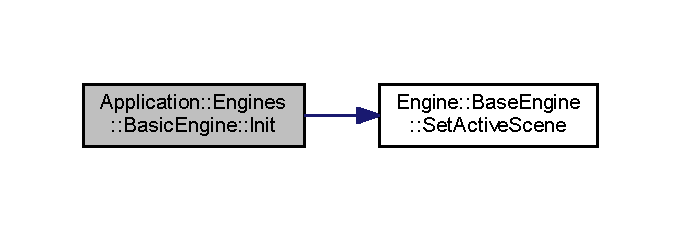
\includegraphics[width=327pt]{classApplication_1_1Engines_1_1BasicEngine_afbdc9f559d1776371f90da00b61ba6ab_cgraph}
\end{center}
\end{figure}
\mbox{\Hypertarget{classEngine_1_1BaseEngine_a7a1c9b833049b3eb61194cab113dfe89}\label{classEngine_1_1BaseEngine_a7a1c9b833049b3eb61194cab113dfe89}} 
\index{Application\+::\+Engines\+::\+Basic\+Engine@{Application\+::\+Engines\+::\+Basic\+Engine}!Init\+Success@{Init\+Success}}
\index{Init\+Success@{Init\+Success}!Application\+::\+Engines\+::\+Basic\+Engine@{Application\+::\+Engines\+::\+Basic\+Engine}}
\subsubsection{\texorpdfstring{Init\+Success()}{InitSuccess()}}
{\footnotesize\ttfamily bool Engine\+::\+Base\+Engine\+::\+Init\+Success (\begin{DoxyParamCaption}{ }\end{DoxyParamCaption})\hspace{0.3cm}{\ttfamily [inherited]}}



Definition at line 46 of file Base\+Engine.\+cpp.


\begin{DoxyCode}
47 \{
48     \textcolor{keywordflow}{return} \mbox{\hyperlink{classEngine_1_1BaseEngine_a79e265845b321c0e9822fb170c564e55}{\_init}};
49 \}
\end{DoxyCode}
\mbox{\Hypertarget{classEngine_1_1BaseEngine_afc82c6a00d5a9d4714740fc5eab5db86}\label{classEngine_1_1BaseEngine_afc82c6a00d5a9d4714740fc5eab5db86}} 
\index{Application\+::\+Engines\+::\+Basic\+Engine@{Application\+::\+Engines\+::\+Basic\+Engine}!Set\+Active\+Scene@{Set\+Active\+Scene}}
\index{Set\+Active\+Scene@{Set\+Active\+Scene}!Application\+::\+Engines\+::\+Basic\+Engine@{Application\+::\+Engines\+::\+Basic\+Engine}}
\subsubsection{\texorpdfstring{Set\+Active\+Scene()}{SetActiveScene()}}
{\footnotesize\ttfamily void Engine\+::\+Base\+Engine\+::\+Set\+Active\+Scene (\begin{DoxyParamCaption}\item[{\mbox{\hyperlink{classEngine_1_1Components_1_1Scene}{Components\+::\+Scene}} $\ast$}]{scene = {\ttfamily nullptr} }\end{DoxyParamCaption})\hspace{0.3cm}{\ttfamily [virtual]}, {\ttfamily [inherited]}}



Definition at line 132 of file Base\+Engine.\+cpp.



Referenced by Init(), Application\+::\+Engines\+::\+Z\+P\+G\+Engine\+::\+Init(), Application\+::\+Engines\+::\+Triangle\+Engine\+::\+Init(), Application\+::\+Engines\+::\+Camera\+Engine\+::\+Init(), and Application\+::\+Engines\+::\+Light\+Engine\+::\+Init().


\begin{DoxyCode}
133 \{
134     \textcolor{keywordflow}{if} (scene == \textcolor{keyword}{nullptr} && !\mbox{\hyperlink{classEngine_1_1BaseEngine_afd02af3c2fbe9bb734db014dec06585a}{Scenes}}->empty())
135         \mbox{\hyperlink{classEngine_1_1BaseEngine_adb3dbc839da9d821e08b18d8a221698d}{ActiveScene}} = \mbox{\hyperlink{classEngine_1_1BaseEngine_afd02af3c2fbe9bb734db014dec06585a}{Scenes}}->begin()->second;
136     \textcolor{keywordflow}{else}
137         \mbox{\hyperlink{classEngine_1_1BaseEngine_adb3dbc839da9d821e08b18d8a221698d}{ActiveScene}} = scene;     
138 \}
\end{DoxyCode}
Here is the caller graph for this function\+:
\nopagebreak
\begin{figure}[H]
\begin{center}
\leavevmode
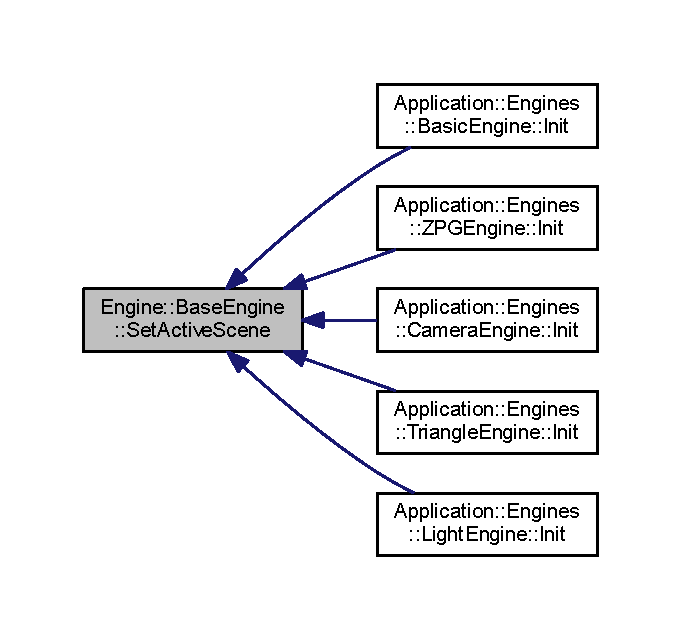
\includegraphics[width=327pt]{classEngine_1_1BaseEngine_afc82c6a00d5a9d4714740fc5eab5db86_icgraph}
\end{center}
\end{figure}
\mbox{\Hypertarget{classEngine_1_1BaseEngine_a525fdc7a1da7eecb514ad5763f06be79}\label{classEngine_1_1BaseEngine_a525fdc7a1da7eecb514ad5763f06be79}} 
\index{Application\+::\+Engines\+::\+Basic\+Engine@{Application\+::\+Engines\+::\+Basic\+Engine}!Start@{Start}}
\index{Start@{Start}!Application\+::\+Engines\+::\+Basic\+Engine@{Application\+::\+Engines\+::\+Basic\+Engine}}
\subsubsection{\texorpdfstring{Start()}{Start()}}
{\footnotesize\ttfamily void Engine\+::\+Base\+Engine\+::\+Start (\begin{DoxyParamCaption}{ }\end{DoxyParamCaption})\hspace{0.3cm}{\ttfamily [virtual]}, {\ttfamily [inherited]}}



Definition at line 126 of file Base\+Engine.\+cpp.



Referenced by main().


\begin{DoxyCode}
127 \{
128     system(\textcolor{stringliteral}{"cls"});
129     \mbox{\hyperlink{classEngine_1_1BaseEngine_aad3c237ca657b9f22f76fccf7fc7561f}{UpdateInternal}}();
130 \}
\end{DoxyCode}
Here is the caller graph for this function\+:
\nopagebreak
\begin{figure}[H]
\begin{center}
\leavevmode
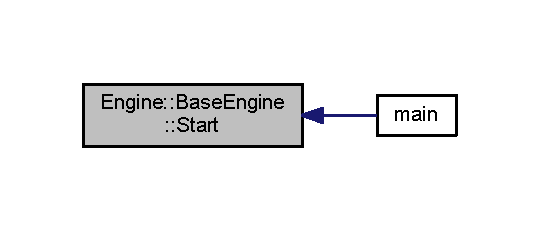
\includegraphics[width=259pt]{classEngine_1_1BaseEngine_a525fdc7a1da7eecb514ad5763f06be79_icgraph}
\end{center}
\end{figure}
\mbox{\Hypertarget{classApplication_1_1Engines_1_1BasicEngine_ad628d9878f5008dd7f7f7743a75d5f17}\label{classApplication_1_1Engines_1_1BasicEngine_ad628d9878f5008dd7f7f7743a75d5f17}} 
\index{Application\+::\+Engines\+::\+Basic\+Engine@{Application\+::\+Engines\+::\+Basic\+Engine}!Update@{Update}}
\index{Update@{Update}!Application\+::\+Engines\+::\+Basic\+Engine@{Application\+::\+Engines\+::\+Basic\+Engine}}
\subsubsection{\texorpdfstring{Update()}{Update()}\hspace{0.1cm}{\footnotesize\ttfamily [1/2]}}
{\footnotesize\ttfamily void Application\+::\+Engines\+::\+Basic\+Engine\+::\+Update (\begin{DoxyParamCaption}\item[{\+::\mbox{\hyperlink{classEngine_1_1Components_1_1Window}{Engine\+::\+Components\+::\+Window}} $\ast$}]{window }\end{DoxyParamCaption})\hspace{0.3cm}{\ttfamily [override]}}



Definition at line 53 of file Basic\+Engine.\+cpp.


\begin{DoxyCode}
54 \{
55     \textcolor{keywordflow}{if}(\mbox{\hyperlink{classEngine_1_1BaseEngine_adb3dbc839da9d821e08b18d8a221698d}{ActiveScene}} != \textcolor{keyword}{nullptr} && \mbox{\hyperlink{classEngine_1_1BaseEngine_adb3dbc839da9d821e08b18d8a221698d}{ActiveScene}}->\mbox{\hyperlink{classEngine_1_1Components_1_1Scene_a23481feabaaa56bf5613765db03af4da}{Objects}} != \textcolor{keyword}{nullptr} && !
      \mbox{\hyperlink{classEngine_1_1BaseEngine_adb3dbc839da9d821e08b18d8a221698d}{ActiveScene}}->\mbox{\hyperlink{classEngine_1_1Components_1_1Scene_a23481feabaaa56bf5613765db03af4da}{Objects}}->empty())
56     \textcolor{keywordflow}{for} (\textcolor{keyword}{auto}& it : *\mbox{\hyperlink{classEngine_1_1BaseEngine_adb3dbc839da9d821e08b18d8a221698d}{ActiveScene}}->\mbox{\hyperlink{classEngine_1_1Components_1_1Scene_a23481feabaaa56bf5613765db03af4da}{Objects}})
57     \{
58         std::cout << \textcolor{stringliteral}{"Object: "} << it.first << std::endl;
59         \textcolor{keyword}{auto} \textcolor{keywordtype}{object} = it.second;
60         \textcolor{keywordtype}{object}->Draw();
61         \mbox{\hyperlink{classApplication_1_1Engines_1_1BasicEngine_aad99e45bc67ec33b4fc26b38b9c8a31e}{angle}} += 0.1f;
62     \}
63 \}
\end{DoxyCode}
\mbox{\Hypertarget{classEngine_1_1BaseEngine_a01c23c2073f08939a660f3b7a866852c}\label{classEngine_1_1BaseEngine_a01c23c2073f08939a660f3b7a866852c}} 
\index{Application\+::\+Engines\+::\+Basic\+Engine@{Application\+::\+Engines\+::\+Basic\+Engine}!Update@{Update}}
\index{Update@{Update}!Application\+::\+Engines\+::\+Basic\+Engine@{Application\+::\+Engines\+::\+Basic\+Engine}}
\subsubsection{\texorpdfstring{Update()}{Update()}\hspace{0.1cm}{\footnotesize\ttfamily [2/2]}}
{\footnotesize\ttfamily void Engine\+::\+Base\+Engine\+::\+Update (\begin{DoxyParamCaption}\item[{\mbox{\hyperlink{classEngine_1_1Components_1_1Window}{Components\+::\+Window}} $\ast$}]{window }\end{DoxyParamCaption})\hspace{0.3cm}{\ttfamily [virtual]}, {\ttfamily [inherited]}}



Definition at line 112 of file Base\+Engine.\+cpp.


\begin{DoxyCode}
113 \{
114 \}
\end{DoxyCode}
\mbox{\Hypertarget{classEngine_1_1BaseEngine_aace6be2a42d12b64fbd35f1acdb08408}\label{classEngine_1_1BaseEngine_aace6be2a42d12b64fbd35f1acdb08408}} 
\index{Application\+::\+Engines\+::\+Basic\+Engine@{Application\+::\+Engines\+::\+Basic\+Engine}!Update\+Begin@{Update\+Begin}}
\index{Update\+Begin@{Update\+Begin}!Application\+::\+Engines\+::\+Basic\+Engine@{Application\+::\+Engines\+::\+Basic\+Engine}}
\subsubsection{\texorpdfstring{Update\+Begin()}{UpdateBegin()}}
{\footnotesize\ttfamily void Engine\+::\+Base\+Engine\+::\+Update\+Begin (\begin{DoxyParamCaption}\item[{\mbox{\hyperlink{classEngine_1_1Components_1_1Window}{Components\+::\+Window}} $\ast$}]{window }\end{DoxyParamCaption})\hspace{0.3cm}{\ttfamily [virtual]}, {\ttfamily [inherited]}}



Definition at line 57 of file Base\+Engine.\+cpp.



References Engine\+::\+Components\+::\+Window\+::\+Get().


\begin{DoxyCode}
58 \{
59     \textcolor{comment}{// Scene}
60     \mbox{\hyperlink{classEngine_1_1BaseEngine_adb3dbc839da9d821e08b18d8a221698d}{ActiveScene}}->\mbox{\hyperlink{classEngine_1_1Components_1_1Scene_af18bd334fe66952b8d79b8e9e99ab2d8}{BeginLoad}}(\textcolor{keyword}{this});
61 
62     \textcolor{comment}{// Buffers}
63     glEnable(GL\_DEPTH\_TEST);
64     glDepthFunc(GL\_LESS);
65     glClear(GL\_COLOR\_BUFFER\_BIT | GL\_DEPTH\_BUFFER\_BIT);
66 
67     \textcolor{comment}{// Input}
68     \textcolor{keywordtype}{short} mouseKeysActive = 0;
69     glfwGetCursorPos(window->Get(), &\mbox{\hyperlink{classEngine_1_1BaseEngine_a5fe085152ebe93346900407f6b41a034}{MouseX}}, &\mbox{\hyperlink{classEngine_1_1BaseEngine_a143c9c32dbbdc70bf1546ffe275bf384}{MouseY}});
70     \textcolor{keywordflow}{for}(\textcolor{keywordtype}{short} i = 0; i < 8; i++)
71     \{
72         \textcolor{keyword}{const} \textcolor{keywordtype}{int} state = glfwGetMouseButton(window->Get(), i);
73         \textcolor{keyword}{auto} value = \mbox{\hyperlink{classEngine_1_1BaseEngine_a3ee2bdddb66d45b8c808ffd937ba9c50}{MouseKeys}}[i];
74         \textcolor{comment}{// flip state}
75         \textcolor{keywordflow}{if} (state == GLFW\_PRESS && !value)
76             \mbox{\hyperlink{classEngine_1_1BaseEngine_a3ee2bdddb66d45b8c808ffd937ba9c50}{MouseKeys}}.\mbox{\hyperlink{classGeneric_1_1Dictionary_ae7cb006f801b21c172e8fbac8794fa99}{Add}}(i, \textcolor{keyword}{true});
77         \textcolor{keywordflow}{else} \textcolor{keywordflow}{if} (state == GLFW\_RELEASE && value)
78             \mbox{\hyperlink{classEngine_1_1BaseEngine_a3ee2bdddb66d45b8c808ffd937ba9c50}{MouseKeys}}.\mbox{\hyperlink{classGeneric_1_1Dictionary_ae7cb006f801b21c172e8fbac8794fa99}{Add}}(i, \textcolor{keyword}{false});
79         \textcolor{keywordflow}{if} (\mbox{\hyperlink{classEngine_1_1BaseEngine_a3ee2bdddb66d45b8c808ffd937ba9c50}{MouseKeys}}[i])
80             mouseKeysActive++;
81     \}
82     \textcolor{keywordtype}{short} keysActive = 0;
83     SetConsoleCursorPosition(GetStdHandle(STD\_OUTPUT\_HANDLE), \{ 40, keysActive \});
84     fprintf(\mbox{\hyperlink{classEngine_1_1BaseEngine_a26fd54a1ee2733f9c654af5afcfa96cf}{\_errorStream}}, \textcolor{stringliteral}{"                           "});
85     \textcolor{keywordflow}{for} (\textcolor{keywordtype}{short} i = 1; i < 512; i++)
86     \{
87         \textcolor{keyword}{const} \textcolor{keywordtype}{int} state = glfwGetKey(window->Get(), i);
88         \textcolor{keyword}{auto} value = \mbox{\hyperlink{classEngine_1_1BaseEngine_a65321a97e83f0a6ee90df3efac2d3307}{Keys}}[i];
89         \textcolor{comment}{// flip state}
90         \textcolor{keywordflow}{if} (state == GLFW\_PRESS && !value)
91             \mbox{\hyperlink{classEngine_1_1BaseEngine_a65321a97e83f0a6ee90df3efac2d3307}{Keys}}.\mbox{\hyperlink{classGeneric_1_1Dictionary_ae7cb006f801b21c172e8fbac8794fa99}{Add}}(i, \textcolor{keyword}{true});
92         \textcolor{keywordflow}{else} \textcolor{keywordflow}{if} (state == GLFW\_RELEASE && value)
93             \mbox{\hyperlink{classEngine_1_1BaseEngine_a65321a97e83f0a6ee90df3efac2d3307}{Keys}}.\mbox{\hyperlink{classGeneric_1_1Dictionary_ae7cb006f801b21c172e8fbac8794fa99}{Add}}(i, \textcolor{keyword}{false});
94         \textcolor{keywordflow}{if} (\mbox{\hyperlink{classEngine_1_1BaseEngine_a65321a97e83f0a6ee90df3efac2d3307}{Keys}}[i])
95             keysActive++;
96     \}
97     \textcolor{keywordtype}{bool} handleKeys = \textcolor{keyword}{true},
98          handleMouse = \textcolor{keyword}{true};
99     \textcolor{keywordflow}{for} (\textcolor{keyword}{auto} handler : *\mbox{\hyperlink{classEngine_1_1BaseEngine_a134fa082c5a64d62b76ddf926647e7cc}{InputHandlers}})
100     \{
101         \textcolor{keywordflow}{if}(handleKeys)
102             handleKeys = handler->HandleKeys(\textcolor{keyword}{this}, window, \mbox{\hyperlink{classEngine_1_1BaseEngine_adb3dbc839da9d821e08b18d8a221698d}{ActiveScene}}, 
      \mbox{\hyperlink{classEngine_1_1BaseEngine_a65321a97e83f0a6ee90df3efac2d3307}{Keys}}, keysActive);
103         \textcolor{keywordflow}{if}(handleMouse)
104             handleMouse = handler->HandleMouse(\textcolor{keyword}{this}, window, \mbox{\hyperlink{classEngine_1_1BaseEngine_adb3dbc839da9d821e08b18d8a221698d}{ActiveScene}}, 
      \mbox{\hyperlink{classEngine_1_1BaseEngine_a5fe085152ebe93346900407f6b41a034}{MouseX}}, \mbox{\hyperlink{classEngine_1_1BaseEngine_a143c9c32dbbdc70bf1546ffe275bf384}{MouseY}}, \mbox{\hyperlink{classEngine_1_1BaseEngine_a3ee2bdddb66d45b8c808ffd937ba9c50}{MouseKeys}}, mouseKeysActive);
105         \textcolor{keywordflow}{if}(!handleKeys && !handleMouse)
106             \textcolor{keywordflow}{break};
107     \}
108 
109     SetConsoleCursorPosition(GetStdHandle(STD\_OUTPUT\_HANDLE), \{ 0,0 \});
110 \}
\end{DoxyCode}
Here is the call graph for this function\+:
\nopagebreak
\begin{figure}[H]
\begin{center}
\leavevmode
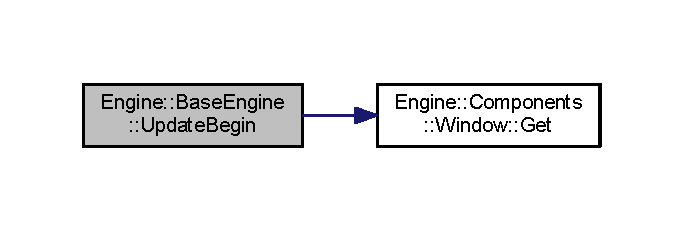
\includegraphics[width=328pt]{classEngine_1_1BaseEngine_aace6be2a42d12b64fbd35f1acdb08408_cgraph}
\end{center}
\end{figure}
\mbox{\Hypertarget{classEngine_1_1BaseEngine_a7c07c98e583df042a0eb01e0ddec85a1}\label{classEngine_1_1BaseEngine_a7c07c98e583df042a0eb01e0ddec85a1}} 
\index{Application\+::\+Engines\+::\+Basic\+Engine@{Application\+::\+Engines\+::\+Basic\+Engine}!Update\+End@{Update\+End}}
\index{Update\+End@{Update\+End}!Application\+::\+Engines\+::\+Basic\+Engine@{Application\+::\+Engines\+::\+Basic\+Engine}}
\subsubsection{\texorpdfstring{Update\+End()}{UpdateEnd()}}
{\footnotesize\ttfamily void Engine\+::\+Base\+Engine\+::\+Update\+End (\begin{DoxyParamCaption}\item[{\mbox{\hyperlink{classEngine_1_1Components_1_1Window}{Components\+::\+Window}} $\ast$}]{window }\end{DoxyParamCaption})\hspace{0.3cm}{\ttfamily [virtual]}, {\ttfamily [inherited]}}



Definition at line 116 of file Base\+Engine.\+cpp.



References Engine\+::\+Components\+::\+Window\+::\+Get().


\begin{DoxyCode}
117 \{
118     \textcolor{comment}{// update other events like input handling}
119     glfwPollEvents();
120     \textcolor{comment}{// put the stuff we’ve been drawing onto the display}
121     glfwSwapBuffers(window->Get());
122 
123     \mbox{\hyperlink{classEngine_1_1BaseEngine_adb3dbc839da9d821e08b18d8a221698d}{ActiveScene}}->\mbox{\hyperlink{classEngine_1_1Components_1_1Scene_abd8fcdcac52dbce6a0a18de3860ab087}{FrameUpdate}}(\textcolor{keyword}{this});
124 \}
\end{DoxyCode}
Here is the call graph for this function\+:
\nopagebreak
\begin{figure}[H]
\begin{center}
\leavevmode
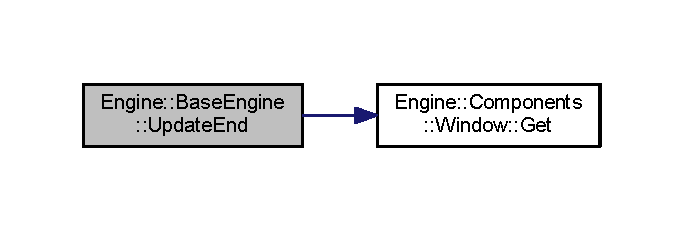
\includegraphics[width=328pt]{classEngine_1_1BaseEngine_a7c07c98e583df042a0eb01e0ddec85a1_cgraph}
\end{center}
\end{figure}


\subsection{Member Data Documentation}
\mbox{\Hypertarget{classEngine_1_1BaseEngine_adb3dbc839da9d821e08b18d8a221698d}\label{classEngine_1_1BaseEngine_adb3dbc839da9d821e08b18d8a221698d}} 
\index{Application\+::\+Engines\+::\+Basic\+Engine@{Application\+::\+Engines\+::\+Basic\+Engine}!Active\+Scene@{Active\+Scene}}
\index{Active\+Scene@{Active\+Scene}!Application\+::\+Engines\+::\+Basic\+Engine@{Application\+::\+Engines\+::\+Basic\+Engine}}
\subsubsection{\texorpdfstring{Active\+Scene}{ActiveScene}}
{\footnotesize\ttfamily Components\+::\+Scene$\ast$ Engine\+::\+Base\+Engine\+::\+Active\+Scene\hspace{0.3cm}{\ttfamily [inherited]}}



Definition at line 34 of file Base\+Engine.\+h.



Referenced by Engine\+::\+Base\+Engine\+::\+Base\+Engine(), Application\+::\+Engines\+::\+Camera\+Engine\+::\+Init(), and Application\+::\+Engines\+::\+Light\+Engine\+::\+Init().

\mbox{\Hypertarget{classApplication_1_1Engines_1_1BasicEngine_aad99e45bc67ec33b4fc26b38b9c8a31e}\label{classApplication_1_1Engines_1_1BasicEngine_aad99e45bc67ec33b4fc26b38b9c8a31e}} 
\index{Application\+::\+Engines\+::\+Basic\+Engine@{Application\+::\+Engines\+::\+Basic\+Engine}!angle@{angle}}
\index{angle@{angle}!Application\+::\+Engines\+::\+Basic\+Engine@{Application\+::\+Engines\+::\+Basic\+Engine}}
\subsubsection{\texorpdfstring{angle}{angle}}
{\footnotesize\ttfamily float Application\+::\+Engines\+::\+Basic\+Engine\+::angle\hspace{0.3cm}{\ttfamily [private]}}



Definition at line 15 of file Basic\+Engine.\+h.



Referenced by Init().

\mbox{\Hypertarget{classEngine_1_1BaseEngine_a134fa082c5a64d62b76ddf926647e7cc}\label{classEngine_1_1BaseEngine_a134fa082c5a64d62b76ddf926647e7cc}} 
\index{Application\+::\+Engines\+::\+Basic\+Engine@{Application\+::\+Engines\+::\+Basic\+Engine}!Input\+Handlers@{Input\+Handlers}}
\index{Input\+Handlers@{Input\+Handlers}!Application\+::\+Engines\+::\+Basic\+Engine@{Application\+::\+Engines\+::\+Basic\+Engine}}
\subsubsection{\texorpdfstring{Input\+Handlers}{InputHandlers}}
{\footnotesize\ttfamily \mbox{\hyperlink{classGeneric_1_1Collection}{Generic\+::\+Collection}}$<$Components\+::\+I\+Input\+Handler$\ast$$>$$\ast$ Engine\+::\+Base\+Engine\+::\+Input\+Handlers\hspace{0.3cm}{\ttfamily [inherited]}}



Definition at line 31 of file Base\+Engine.\+h.



Referenced by Engine\+::\+Base\+Engine\+::\+Base\+Engine(), and Application\+::\+Engines\+::\+Light\+Engine\+::\+Init().

\mbox{\Hypertarget{classEngine_1_1BaseEngine_a65321a97e83f0a6ee90df3efac2d3307}\label{classEngine_1_1BaseEngine_a65321a97e83f0a6ee90df3efac2d3307}} 
\index{Application\+::\+Engines\+::\+Basic\+Engine@{Application\+::\+Engines\+::\+Basic\+Engine}!Keys@{Keys}}
\index{Keys@{Keys}!Application\+::\+Engines\+::\+Basic\+Engine@{Application\+::\+Engines\+::\+Basic\+Engine}}
\subsubsection{\texorpdfstring{Keys}{Keys}}
{\footnotesize\ttfamily \mbox{\hyperlink{classGeneric_1_1Dictionary}{Generic\+::\+Dictionary}}$<$short, bool$>$ Engine\+::\+Base\+Engine\+::\+Keys\hspace{0.3cm}{\ttfamily [inherited]}}



Definition at line 32 of file Base\+Engine.\+h.



Referenced by Engine\+::\+Base\+Engine\+::\+Base\+Engine().

\mbox{\Hypertarget{classApplication_1_1Engines_1_1BasicEngine_a645ebb7fc6a7eb2961a5c15986a0c246}\label{classApplication_1_1Engines_1_1BasicEngine_a645ebb7fc6a7eb2961a5c15986a0c246}} 
\index{Application\+::\+Engines\+::\+Basic\+Engine@{Application\+::\+Engines\+::\+Basic\+Engine}!M@{M}}
\index{M@{M}!Application\+::\+Engines\+::\+Basic\+Engine@{Application\+::\+Engines\+::\+Basic\+Engine}}
\subsubsection{\texorpdfstring{M}{M}}
{\footnotesize\ttfamily glm\+::mat4 Application\+::\+Engines\+::\+Basic\+Engine\+::M\hspace{0.3cm}{\ttfamily [private]}}



Definition at line 14 of file Basic\+Engine.\+h.



Referenced by Init().

\mbox{\Hypertarget{classEngine_1_1BaseEngine_a3ee2bdddb66d45b8c808ffd937ba9c50}\label{classEngine_1_1BaseEngine_a3ee2bdddb66d45b8c808ffd937ba9c50}} 
\index{Application\+::\+Engines\+::\+Basic\+Engine@{Application\+::\+Engines\+::\+Basic\+Engine}!Mouse\+Keys@{Mouse\+Keys}}
\index{Mouse\+Keys@{Mouse\+Keys}!Application\+::\+Engines\+::\+Basic\+Engine@{Application\+::\+Engines\+::\+Basic\+Engine}}
\subsubsection{\texorpdfstring{Mouse\+Keys}{MouseKeys}}
{\footnotesize\ttfamily \mbox{\hyperlink{classGeneric_1_1Dictionary}{Generic\+::\+Dictionary}}$<$short, bool$>$ Engine\+::\+Base\+Engine\+::\+Mouse\+Keys\hspace{0.3cm}{\ttfamily [inherited]}}



Definition at line 33 of file Base\+Engine.\+h.



Referenced by Engine\+::\+Base\+Engine\+::\+Base\+Engine().

\mbox{\Hypertarget{classEngine_1_1BaseEngine_a5fe085152ebe93346900407f6b41a034}\label{classEngine_1_1BaseEngine_a5fe085152ebe93346900407f6b41a034}} 
\index{Application\+::\+Engines\+::\+Basic\+Engine@{Application\+::\+Engines\+::\+Basic\+Engine}!MouseX@{MouseX}}
\index{MouseX@{MouseX}!Application\+::\+Engines\+::\+Basic\+Engine@{Application\+::\+Engines\+::\+Basic\+Engine}}
\subsubsection{\texorpdfstring{MouseX}{MouseX}}
{\footnotesize\ttfamily double Engine\+::\+Base\+Engine\+::\+MouseX\hspace{0.3cm}{\ttfamily [inherited]}}



Definition at line 35 of file Base\+Engine.\+h.

\mbox{\Hypertarget{classEngine_1_1BaseEngine_a143c9c32dbbdc70bf1546ffe275bf384}\label{classEngine_1_1BaseEngine_a143c9c32dbbdc70bf1546ffe275bf384}} 
\index{Application\+::\+Engines\+::\+Basic\+Engine@{Application\+::\+Engines\+::\+Basic\+Engine}!MouseY@{MouseY}}
\index{MouseY@{MouseY}!Application\+::\+Engines\+::\+Basic\+Engine@{Application\+::\+Engines\+::\+Basic\+Engine}}
\subsubsection{\texorpdfstring{MouseY}{MouseY}}
{\footnotesize\ttfamily double Engine\+::\+Base\+Engine\+::\+MouseY\hspace{0.3cm}{\ttfamily [inherited]}}



Definition at line 36 of file Base\+Engine.\+h.

\mbox{\Hypertarget{classEngine_1_1BaseEngine_ae0f86360ea3a384caefe443dd8f88601}\label{classEngine_1_1BaseEngine_ae0f86360ea3a384caefe443dd8f88601}} 
\index{Application\+::\+Engines\+::\+Basic\+Engine@{Application\+::\+Engines\+::\+Basic\+Engine}!Programs@{Programs}}
\index{Programs@{Programs}!Application\+::\+Engines\+::\+Basic\+Engine@{Application\+::\+Engines\+::\+Basic\+Engine}}
\subsubsection{\texorpdfstring{Programs}{Programs}}
{\footnotesize\ttfamily \mbox{\hyperlink{classGeneric_1_1Dictionary}{Generic\+::\+Dictionary}}$<$std\+::string, Components\+::\+Graphics\+::\+Program$\ast$$>$$\ast$ Engine\+::\+Base\+Engine\+::\+Programs\hspace{0.3cm}{\ttfamily [inherited]}}



Definition at line 28 of file Base\+Engine.\+h.



Referenced by Engine\+::\+Base\+Engine\+::\+Base\+Engine(), Application\+::\+Input\+::\+Handlers\+::\+Camera\+Input\+Handler\+::\+Handle\+Mouse(), Application\+::\+Engines\+::\+Z\+P\+G\+Engine\+::\+Init(), Application\+::\+Engines\+::\+Triangle\+Engine\+::\+Init(), Init(), Application\+::\+Engines\+::\+Camera\+Engine\+::\+Init(), Application\+::\+Engines\+::\+Light\+Engine\+::\+Init(), Application\+::\+Scenes\+::\+Triangle\+Scene\+::\+Load(), and Application\+::\+Scenes\+::\+Sphere\+Scene\+::\+Load().

\mbox{\Hypertarget{classEngine_1_1BaseEngine_afd02af3c2fbe9bb734db014dec06585a}\label{classEngine_1_1BaseEngine_afd02af3c2fbe9bb734db014dec06585a}} 
\index{Application\+::\+Engines\+::\+Basic\+Engine@{Application\+::\+Engines\+::\+Basic\+Engine}!Scenes@{Scenes}}
\index{Scenes@{Scenes}!Application\+::\+Engines\+::\+Basic\+Engine@{Application\+::\+Engines\+::\+Basic\+Engine}}
\subsubsection{\texorpdfstring{Scenes}{Scenes}}
{\footnotesize\ttfamily \mbox{\hyperlink{classGeneric_1_1Dictionary}{Generic\+::\+Dictionary}}$<$std\+::string, Components\+::\+Scene$\ast$$>$$\ast$ Engine\+::\+Base\+Engine\+::\+Scenes\hspace{0.3cm}{\ttfamily [inherited]}}



Definition at line 30 of file Base\+Engine.\+h.



Referenced by Engine\+::\+Base\+Engine\+::\+Base\+Engine(), Application\+::\+Engines\+::\+Z\+P\+G\+Engine\+::\+Init(), Application\+::\+Engines\+::\+Triangle\+Engine\+::\+Init(), Init(), Application\+::\+Engines\+::\+Camera\+Engine\+::\+Init(), and Application\+::\+Engines\+::\+Light\+Engine\+::\+Init().

\mbox{\Hypertarget{classEngine_1_1BaseEngine_a2582dee3f73da82bb422b43317b85e3b}\label{classEngine_1_1BaseEngine_a2582dee3f73da82bb422b43317b85e3b}} 
\index{Application\+::\+Engines\+::\+Basic\+Engine@{Application\+::\+Engines\+::\+Basic\+Engine}!Shaders@{Shaders}}
\index{Shaders@{Shaders}!Application\+::\+Engines\+::\+Basic\+Engine@{Application\+::\+Engines\+::\+Basic\+Engine}}
\subsubsection{\texorpdfstring{Shaders}{Shaders}}
{\footnotesize\ttfamily \mbox{\hyperlink{classGeneric_1_1Dictionary}{Generic\+::\+Dictionary}}$<$std\+::string, Components\+::\+Graphics\+::\+Shader$\ast$$>$$\ast$ Engine\+::\+Base\+Engine\+::\+Shaders\hspace{0.3cm}{\ttfamily [inherited]}}



Definition at line 29 of file Base\+Engine.\+h.



Referenced by Engine\+::\+Base\+Engine\+::\+Base\+Engine(), Application\+::\+Input\+::\+Handlers\+::\+Camera\+Input\+Handler\+::\+Handle\+Mouse(), Application\+::\+Engines\+::\+Triangle\+Engine\+::\+Init(), Application\+::\+Engines\+::\+Z\+P\+G\+Engine\+::\+Init(), Init(), Application\+::\+Engines\+::\+Camera\+Engine\+::\+Init(), and Application\+::\+Engines\+::\+Light\+Engine\+::\+Init().

\mbox{\Hypertarget{classEngine_1_1BaseEngine_a4a1a4c4dae052e66ecc4f326eeed4d33}\label{classEngine_1_1BaseEngine_a4a1a4c4dae052e66ecc4f326eeed4d33}} 
\index{Application\+::\+Engines\+::\+Basic\+Engine@{Application\+::\+Engines\+::\+Basic\+Engine}!Windows@{Windows}}
\index{Windows@{Windows}!Application\+::\+Engines\+::\+Basic\+Engine@{Application\+::\+Engines\+::\+Basic\+Engine}}
\subsubsection{\texorpdfstring{Windows}{Windows}}
{\footnotesize\ttfamily \mbox{\hyperlink{classGeneric_1_1Dictionary}{Generic\+::\+Dictionary}}$<$std\+::string, Components\+::\+Window$\ast$$>$$\ast$ Engine\+::\+Base\+Engine\+::\+Windows\hspace{0.3cm}{\ttfamily [inherited]}}



Definition at line 27 of file Base\+Engine.\+h.



Referenced by Engine\+::\+Base\+Engine\+::\+Base\+Engine(), Application\+::\+Engines\+::\+Z\+P\+G\+Engine\+::\+Init(), Application\+::\+Engines\+::\+Triangle\+Engine\+::\+Init(), Init(), Application\+::\+Engines\+::\+Camera\+Engine\+::\+Init(), and Application\+::\+Engines\+::\+Light\+Engine\+::\+Init().



The documentation for this class was generated from the following files\+:\begin{DoxyCompactItemize}
\item 
Z\+P\+G/\mbox{\hyperlink{BasicEngine_8h}{Basic\+Engine.\+h}}\item 
Z\+P\+G/\mbox{\hyperlink{BasicEngine_8cpp}{Basic\+Engine.\+cpp}}\end{DoxyCompactItemize}

\hypertarget{classApplication_1_1Engines_1_1CameraEngine}{}\section{Application\+:\+:Engines\+:\+:Camera\+Engine Class Reference}
\label{classApplication_1_1Engines_1_1CameraEngine}\index{Application\+::\+Engines\+::\+Camera\+Engine@{Application\+::\+Engines\+::\+Camera\+Engine}}


{\ttfamily \#include $<$Camera\+Engine.\+h$>$}



Inheritance diagram for Application\+:\+:Engines\+:\+:Camera\+Engine\+:
\nopagebreak
\begin{figure}[H]
\begin{center}
\leavevmode
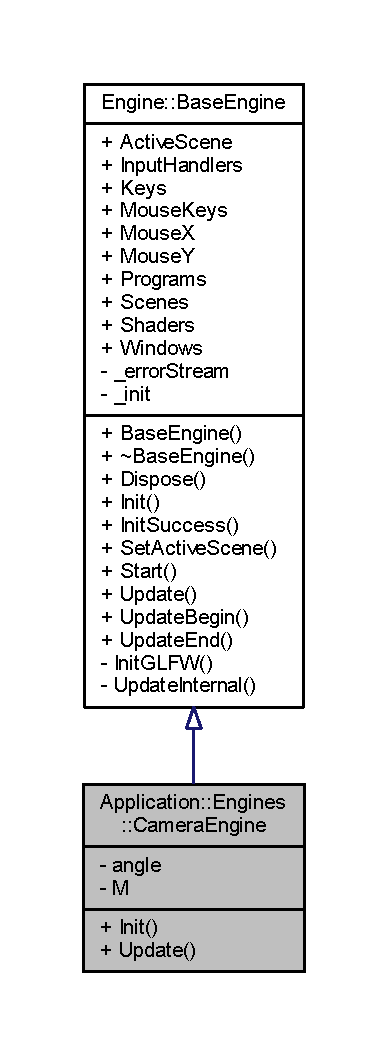
\includegraphics[width=186pt]{classApplication_1_1Engines_1_1CameraEngine__inherit__graph}
\end{center}
\end{figure}


Collaboration diagram for Application\+:\+:Engines\+:\+:Camera\+Engine\+:
\nopagebreak
\begin{figure}[H]
\begin{center}
\leavevmode
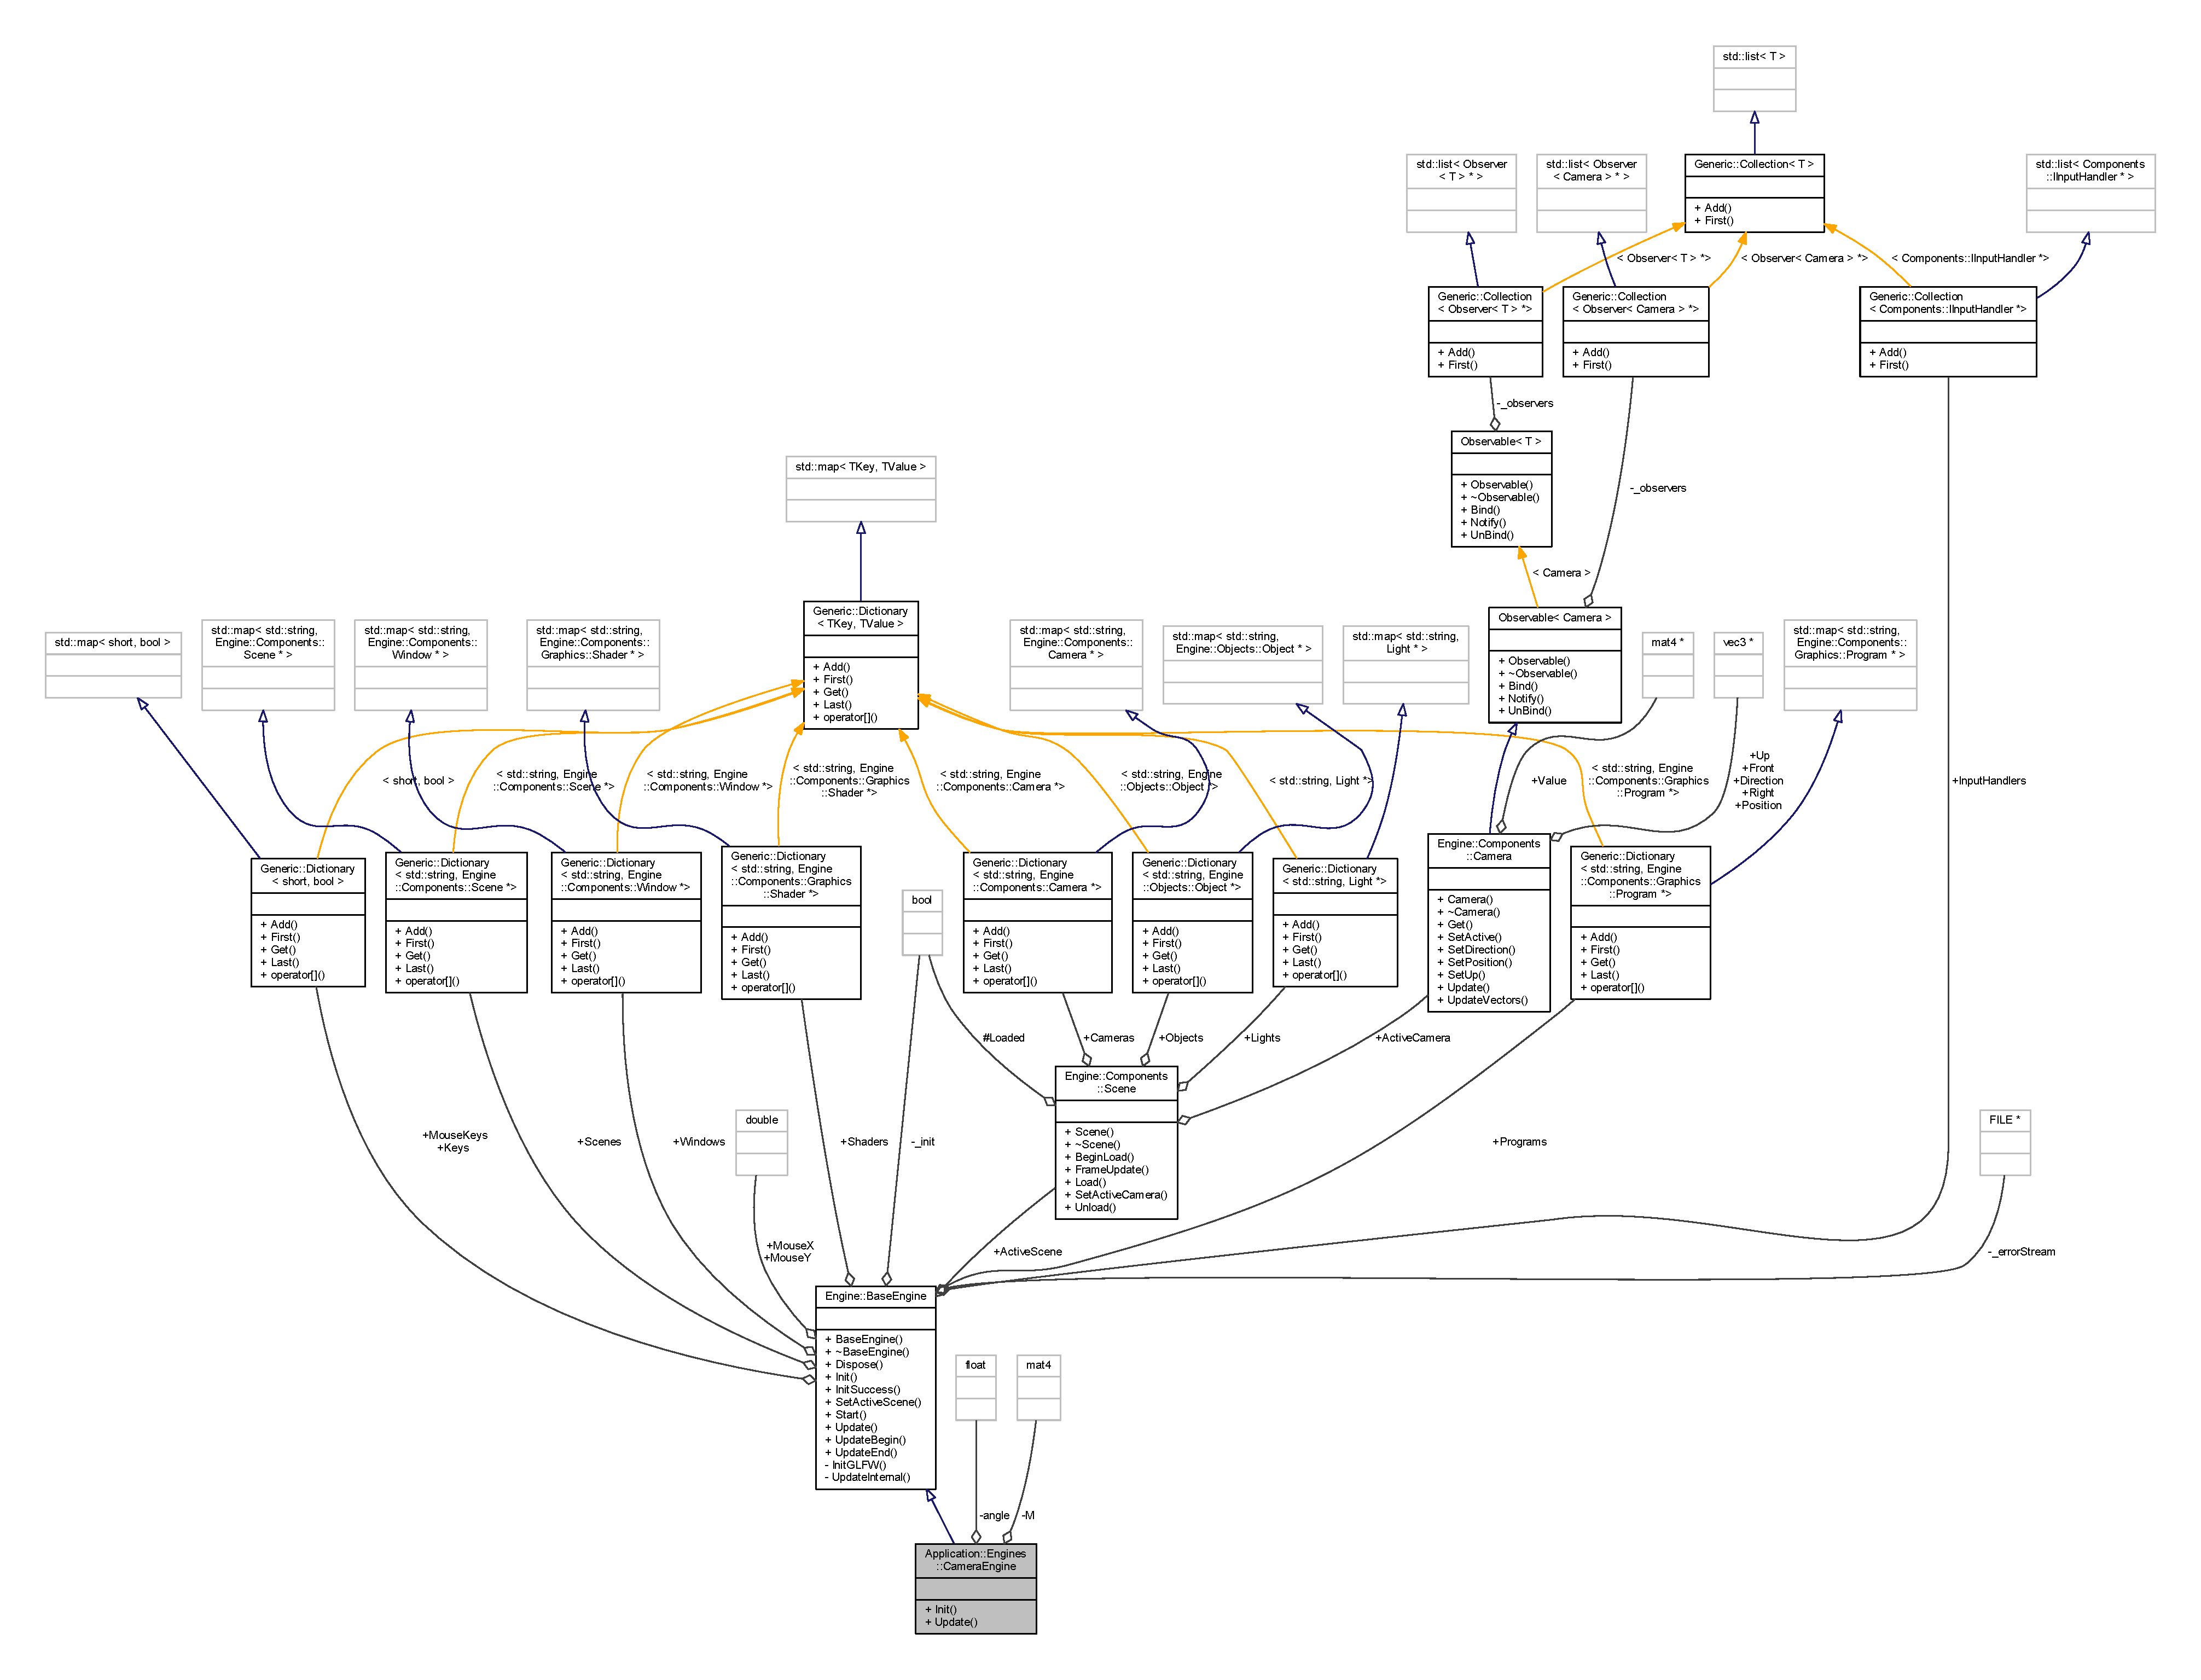
\includegraphics[width=350pt]{classApplication_1_1Engines_1_1CameraEngine__coll__graph}
\end{center}
\end{figure}
\subsection*{Public Member Functions}
\begin{DoxyCompactItemize}
\item 
\mbox{\hyperlink{classEngine_1_1BaseEngine_ad838c97afe1790cb35527f0b58e81e6b}{Base\+Engine}} $\ast$ \mbox{\hyperlink{classEngine_1_1BaseEngine_acd5cd5d2189d24e038b23477b7dce405}{Dispose}} ()
\item 
\mbox{\hyperlink{classApplication_1_1Engines_1_1CameraEngine}{Camera\+Engine}} $\ast$ \mbox{\hyperlink{classApplication_1_1Engines_1_1CameraEngine_a0c7723b93afbdef70394961a4624813d}{Init}} (std\+::\+F\+I\+LE $\ast$error\+Stream=stderr) override
\item 
bool \mbox{\hyperlink{classEngine_1_1BaseEngine_a7a1c9b833049b3eb61194cab113dfe89}{Init\+Success}} ()
\item 
virtual void \mbox{\hyperlink{classEngine_1_1BaseEngine_afc82c6a00d5a9d4714740fc5eab5db86}{Set\+Active\+Scene}} (Components\+::\+Scene $\ast$scene=nullptr)
\item 
virtual void \mbox{\hyperlink{classEngine_1_1BaseEngine_a525fdc7a1da7eecb514ad5763f06be79}{Start}} ()
\item 
void \mbox{\hyperlink{classApplication_1_1Engines_1_1CameraEngine_a48f10aa5b7d87545f5c04d69c37df665}{Update}} (\+::\mbox{\hyperlink{classEngine_1_1Components_1_1Window}{Engine\+::\+Components\+::\+Window}} $\ast$window) override
\item 
virtual void \mbox{\hyperlink{classEngine_1_1BaseEngine_a01c23c2073f08939a660f3b7a866852c}{Update}} (Components\+::\+Window $\ast$window)
\item 
virtual void \mbox{\hyperlink{classEngine_1_1BaseEngine_aace6be2a42d12b64fbd35f1acdb08408}{Update\+Begin}} (Components\+::\+Window $\ast$window)
\item 
virtual void \mbox{\hyperlink{classEngine_1_1BaseEngine_a7c07c98e583df042a0eb01e0ddec85a1}{Update\+End}} (Components\+::\+Window $\ast$window)
\end{DoxyCompactItemize}
\subsection*{Public Attributes}
\begin{DoxyCompactItemize}
\item 
Components\+::\+Scene $\ast$ \mbox{\hyperlink{classEngine_1_1BaseEngine_adb3dbc839da9d821e08b18d8a221698d}{Active\+Scene}}
\item 
\mbox{\hyperlink{classGeneric_1_1Collection}{Generic\+::\+Collection}}$<$ Components\+::\+I\+Input\+Handler $\ast$ $>$ $\ast$ \mbox{\hyperlink{classEngine_1_1BaseEngine_a134fa082c5a64d62b76ddf926647e7cc}{Input\+Handlers}}
\item 
\mbox{\hyperlink{classGeneric_1_1Dictionary}{Generic\+::\+Dictionary}}$<$ short, bool $>$ \mbox{\hyperlink{classEngine_1_1BaseEngine_a65321a97e83f0a6ee90df3efac2d3307}{Keys}}
\item 
\mbox{\hyperlink{classGeneric_1_1Dictionary}{Generic\+::\+Dictionary}}$<$ short, bool $>$ \mbox{\hyperlink{classEngine_1_1BaseEngine_a3ee2bdddb66d45b8c808ffd937ba9c50}{Mouse\+Keys}}
\item 
double \mbox{\hyperlink{classEngine_1_1BaseEngine_a5fe085152ebe93346900407f6b41a034}{MouseX}}
\item 
double \mbox{\hyperlink{classEngine_1_1BaseEngine_a143c9c32dbbdc70bf1546ffe275bf384}{MouseY}}
\item 
\mbox{\hyperlink{classGeneric_1_1Dictionary}{Generic\+::\+Dictionary}}$<$ std\+::string, Components\+::\+Graphics\+::\+Program $\ast$ $>$ $\ast$ \mbox{\hyperlink{classEngine_1_1BaseEngine_ae0f86360ea3a384caefe443dd8f88601}{Programs}}
\item 
\mbox{\hyperlink{classGeneric_1_1Dictionary}{Generic\+::\+Dictionary}}$<$ std\+::string, Components\+::\+Scene $\ast$ $>$ $\ast$ \mbox{\hyperlink{classEngine_1_1BaseEngine_afd02af3c2fbe9bb734db014dec06585a}{Scenes}}
\item 
\mbox{\hyperlink{classGeneric_1_1Dictionary}{Generic\+::\+Dictionary}}$<$ std\+::string, Components\+::\+Graphics\+::\+Shader $\ast$ $>$ $\ast$ \mbox{\hyperlink{classEngine_1_1BaseEngine_a2582dee3f73da82bb422b43317b85e3b}{Shaders}}
\item 
\mbox{\hyperlink{classGeneric_1_1Dictionary}{Generic\+::\+Dictionary}}$<$ std\+::string, Components\+::\+Window $\ast$ $>$ $\ast$ \mbox{\hyperlink{classEngine_1_1BaseEngine_a4a1a4c4dae052e66ecc4f326eeed4d33}{Windows}}
\end{DoxyCompactItemize}
\subsection*{Private Attributes}
\begin{DoxyCompactItemize}
\item 
float \mbox{\hyperlink{classApplication_1_1Engines_1_1CameraEngine_a5298e9f5fa1a2984e21274c4524f771c}{angle}}
\item 
glm\+::mat4 \mbox{\hyperlink{classApplication_1_1Engines_1_1CameraEngine_a2c5eb2ee7aa78a335df64d77242fb21c}{M}}
\end{DoxyCompactItemize}


\subsection{Detailed Description}


Definition at line 8 of file Camera\+Engine.\+h.



\subsection{Member Function Documentation}
\mbox{\Hypertarget{classEngine_1_1BaseEngine_acd5cd5d2189d24e038b23477b7dce405}\label{classEngine_1_1BaseEngine_acd5cd5d2189d24e038b23477b7dce405}} 
\index{Application\+::\+Engines\+::\+Camera\+Engine@{Application\+::\+Engines\+::\+Camera\+Engine}!Dispose@{Dispose}}
\index{Dispose@{Dispose}!Application\+::\+Engines\+::\+Camera\+Engine@{Application\+::\+Engines\+::\+Camera\+Engine}}
\subsubsection{\texorpdfstring{Dispose()}{Dispose()}}
{\footnotesize\ttfamily \mbox{\hyperlink{classEngine_1_1BaseEngine}{Engine\+::\+Base\+Engine}} $\ast$ Engine\+::\+Base\+Engine\+::\+Dispose (\begin{DoxyParamCaption}{ }\end{DoxyParamCaption})\hspace{0.3cm}{\ttfamily [inherited]}}



Definition at line 51 of file Base\+Engine.\+cpp.


\begin{DoxyCode}
52 \{
53     glfwTerminate();
54     \textcolor{keywordflow}{return} \textcolor{keyword}{this};
55 \}
\end{DoxyCode}
\mbox{\Hypertarget{classApplication_1_1Engines_1_1CameraEngine_a0c7723b93afbdef70394961a4624813d}\label{classApplication_1_1Engines_1_1CameraEngine_a0c7723b93afbdef70394961a4624813d}} 
\index{Application\+::\+Engines\+::\+Camera\+Engine@{Application\+::\+Engines\+::\+Camera\+Engine}!Init@{Init}}
\index{Init@{Init}!Application\+::\+Engines\+::\+Camera\+Engine@{Application\+::\+Engines\+::\+Camera\+Engine}}
\subsubsection{\texorpdfstring{Init()}{Init()}}
{\footnotesize\ttfamily \mbox{\hyperlink{classApplication_1_1Engines_1_1CameraEngine}{Application\+::\+Engines\+::\+Camera\+Engine}} $\ast$ Application\+::\+Engines\+::\+Camera\+Engine\+::\+Init (\begin{DoxyParamCaption}\item[{std\+::\+F\+I\+LE $\ast$}]{error\+Stream = {\ttfamily stderr} }\end{DoxyParamCaption})\hspace{0.3cm}{\ttfamily [override]}, {\ttfamily [virtual]}}



Reimplemented from \mbox{\hyperlink{classEngine_1_1BaseEngine_ad9c141fe48c8c91e14e77ed5fcb90196}{Engine\+::\+Base\+Engine}}.



Definition at line 9 of file Camera\+Engine.\+cpp.



References Engine\+::\+Base\+Engine\+::\+Active\+Scene, angle, Engine\+::\+Components\+::\+Scene\+::\+Begin\+Load(), Engine\+::\+Components\+::\+Scene\+::\+Cameras, Generic\+::\+Dictionary$<$ T\+Key, T\+Value $>$\+::\+First(), fragment\+\_\+shader, M, Engine\+::\+Components\+::\+Objects\+::\+Vertex\+Object\+::\+Material, Engine\+::\+Components\+::\+Scene\+::\+Objects, Engine\+::\+Base\+Engine\+::\+Programs, Engine\+::\+Base\+Engine\+::\+Scenes, Engine\+::\+Base\+Engine\+::\+Set\+Active\+Scene(), Engine\+::\+Base\+Engine\+::\+Shaders, Assets\+::\+Shaders\+Fragment, Assets\+::\+Shaders\+Vertex, Engine\+::\+Components\+::\+Graphics\+::\+Material\+::\+Values, vertex\+\_\+shader, and Engine\+::\+Base\+Engine\+::\+Windows.


\begin{DoxyCode}
10 \{
11     BaseEngine::Init(errorStream);
12 
13     \textcolor{keyword}{const} \textcolor{keywordtype}{char}* \mbox{\hyperlink{ZPGEngine_8cpp_afc33b8912f9f93d1d2544df04ad4a81a}{vertex\_shader}} =
14         \textcolor{stringliteral}{"#version 330\(\backslash\)n"}
15         \textcolor{stringliteral}{"layout(location=0) in vec3 vp;"}
16         \textcolor{stringliteral}{"out vec3 ex\_WorldPos;"}
17         \textcolor{stringliteral}{"uniform mat4 modelMatrix;"}
18         \textcolor{stringliteral}{"uniform mat4 viewMatrix;"}
19         \textcolor{stringliteral}{"uniform mat4 projectionMatrix;"}
20         \textcolor{stringliteral}{"void main () \{"}
21         \textcolor{stringliteral}{" gl\_Position = (projectionMatrix * viewMatrix * modelMatrix) * vec4 (vp, 1.0);"}
22         \textcolor{stringliteral}{"\}"};
23 
24     \textcolor{keyword}{const} \textcolor{keywordtype}{char}* \mbox{\hyperlink{ZPGEngine_8cpp_ab187f2ba2a2f72ea5571921a1a856582}{fragment\_shader}} =
25         \textcolor{stringliteral}{"#version 330\(\backslash\)n"}
26         \textcolor{stringliteral}{"uniform float color;"}
27         \textcolor{stringliteral}{"out vec4 frag\_colour;"}
28         \textcolor{stringliteral}{"void main () \{"}
29         \textcolor{stringliteral}{"     frag\_colour = vec4 (color, 1.0-color, 0.0, 1.0);"}
30         \textcolor{stringliteral}{"\}"};
31 
32     \mbox{\hyperlink{classApplication_1_1Engines_1_1CameraEngine_a2c5eb2ee7aa78a335df64d77242fb21c}{M}} = glm::mat4(1.0f);
33     \mbox{\hyperlink{classApplication_1_1Engines_1_1CameraEngine_a5298e9f5fa1a2984e21274c4524f771c}{angle}} = 0.0f;
34 
35     \mbox{\hyperlink{classEngine_1_1BaseEngine_a4a1a4c4dae052e66ecc4f326eeed4d33}{Windows}}->Add(\textcolor{stringliteral}{"zpg"}, (new ::Engine::Components::Window(800, 600, \textcolor{stringliteral}{"ZPG - Camera"}, 100.0f))
36         ->Show()
37         ->Info(std::cout)
38     );
39 
40     \textcolor{keyword}{auto}* vertex = \textcolor{keyword}{new} \mbox{\hyperlink{classEngine_1_1Components_1_1Graphics_1_1Shader}{Engine::Components::Graphics::Shader}}(
      GL\_VERTEX\_SHADER, \mbox{\hyperlink{classAssets_ac712d5aca276086a3734e2e9f74cfc6b}{Assets::ShadersVertex}} + \textcolor{stringliteral}{"Camera.glsl"});
41     \mbox{\hyperlink{classEngine_1_1BaseEngine_a2582dee3f73da82bb422b43317b85e3b}{Shaders}}->Add(\textcolor{stringliteral}{"vertex"}, vertex);
42     \mbox{\hyperlink{classEngine_1_1BaseEngine_a2582dee3f73da82bb422b43317b85e3b}{Shaders}}->Add(\textcolor{stringliteral}{"fragment"}, \textcolor{keyword}{new} \mbox{\hyperlink{classEngine_1_1Components_1_1Graphics_1_1Shader}{Engine::Components::Graphics::Shader}}
      (GL\_FRAGMENT\_SHADER, \mbox{\hyperlink{classAssets_abb1ca75a8a9c7b942232df4aff9bb6c9}{Assets::ShadersFragment}} + \textcolor{stringliteral}{"Basic.glsl"}));
43 
44     \mbox{\hyperlink{classEngine_1_1BaseEngine_ae0f86360ea3a384caefe443dd8f88601}{Programs}}->Add(\textcolor{stringliteral}{"basic"}, (\textcolor{keyword}{new} \mbox{\hyperlink{classEngine_1_1Components_1_1Graphics_1_1Program}{Engine::Components::Graphics::Program}}
      ())->AddShaders(\mbox{\hyperlink{classEngine_1_1BaseEngine_a2582dee3f73da82bb422b43317b85e3b}{Shaders}}));
45 
46     \mbox{\hyperlink{classEngine_1_1BaseEngine_afd02af3c2fbe9bb734db014dec06585a}{Scenes}}->Add(\textcolor{stringliteral}{"triangle"}, \textcolor{keyword}{new} Scenes::TriangleScene());
47     \mbox{\hyperlink{classEngine_1_1BaseEngine_afd02af3c2fbe9bb734db014dec06585a}{Scenes}}->Add(\textcolor{stringliteral}{"sphere"}, \textcolor{keyword}{new} Scenes::SphereScene());
48 
49     \mbox{\hyperlink{classEngine_1_1BaseEngine_afc82c6a00d5a9d4714740fc5eab5db86}{SetActiveScene}}(\mbox{\hyperlink{classEngine_1_1BaseEngine_afd02af3c2fbe9bb734db014dec06585a}{Scenes}}->Get(\textcolor{stringliteral}{"sphere"}));
50 
51     \mbox{\hyperlink{classEngine_1_1BaseEngine_adb3dbc839da9d821e08b18d8a221698d}{ActiveScene}}->\mbox{\hyperlink{classEngine_1_1Components_1_1Scene_af18bd334fe66952b8d79b8e9e99ab2d8}{BeginLoad}}(\textcolor{keyword}{this});
52 
53     \mbox{\hyperlink{classEngine_1_1BaseEngine_adb3dbc839da9d821e08b18d8a221698d}{ActiveScene}}->\mbox{\hyperlink{classEngine_1_1Components_1_1Scene_aea98ff1ced88ee859878b504e9a2a362}{Cameras}}->Add(\textcolor{stringliteral}{"main"}, (\textcolor{keyword}{new} 
      \mbox{\hyperlink{classEngine_1_1Components_1_1Camera}{Engine::Components::Camera}}())
54 \textcolor{comment}{//      ->SetPosition(new glm::vec3(2.5f, 2.5f, 2.f))}
55         ->SetPosition(\textcolor{keyword}{new} glm::vec3(0.f, 1.5f, 4.f))
56         ->SetDirection(\textcolor{keyword}{new} glm::vec3(0.f, 0.f, 0.f))
57         ->SetUp(\textcolor{keyword}{new} glm::vec3(0.f, 0.f, 1.f)));
58 
59     \mbox{\hyperlink{classEngine_1_1BaseEngine_adb3dbc839da9d821e08b18d8a221698d}{ActiveScene}}->\mbox{\hyperlink{classEngine_1_1Components_1_1Scene_a23481feabaaa56bf5613765db03af4da}{Objects}}->\mbox{\hyperlink{classGeneric_1_1Dictionary_ab368d54de28e7a3514e1add4bb5b3a36}{First}}()
60         ->\mbox{\hyperlink{classEngine_1_1Components_1_1Objects_1_1VertexObject_a86c1fced4cdc5e59a66a635390a17eca}{Material}}->\mbox{\hyperlink{classEngine_1_1Components_1_1Graphics_1_1Material_a34335608ba1e6eb2c2dba5032107eab0}{Values}}
61         ->Add(
62             \textcolor{keyword}{new} \mbox{\hyperlink{classEngine_1_1Components_1_1Graphics_1_1MaterialValue}{Engine::Components::Graphics::MaterialValue<glm::mat4>}}
      (
63                 vertex,
64                 \textcolor{stringliteral}{"viewMatrix"},
65                 \mbox{\hyperlink{classEngine_1_1BaseEngine_adb3dbc839da9d821e08b18d8a221698d}{ActiveScene}}->\mbox{\hyperlink{classEngine_1_1Components_1_1Scene_aea98ff1ced88ee859878b504e9a2a362}{Cameras}}->First()->Value)
66         ).Add(
67             \textcolor{keyword}{new} \mbox{\hyperlink{classEngine_1_1Components_1_1Graphics_1_1MaterialValue}{Engine::Components::Graphics::MaterialValue<glm::mat4>}}
      (
68                 vertex,
69                 \textcolor{stringliteral}{"projectionMatrix"},
70                 \textcolor{keyword}{new} glm::mat4(glm::perspective(glm::radians(90.0f), 4.0f / 3.0f, 0.1f, 100.0f)))
71         );
72     \textcolor{keywordflow}{return} \textcolor{keyword}{this};
73 \}
\end{DoxyCode}
Here is the call graph for this function\+:
\nopagebreak
\begin{figure}[H]
\begin{center}
\leavevmode
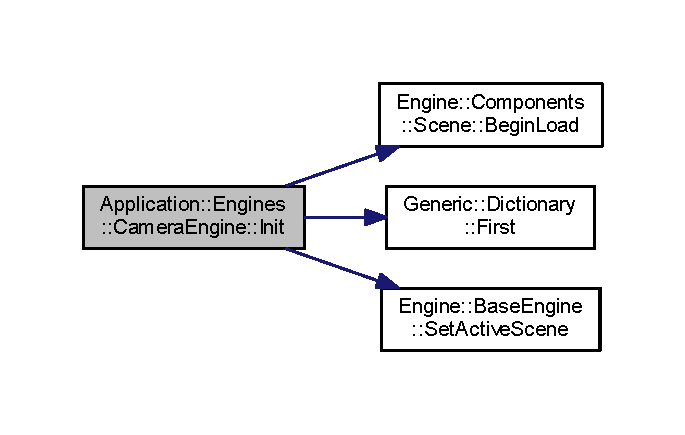
\includegraphics[width=329pt]{classApplication_1_1Engines_1_1CameraEngine_a0c7723b93afbdef70394961a4624813d_cgraph}
\end{center}
\end{figure}
\mbox{\Hypertarget{classEngine_1_1BaseEngine_a7a1c9b833049b3eb61194cab113dfe89}\label{classEngine_1_1BaseEngine_a7a1c9b833049b3eb61194cab113dfe89}} 
\index{Application\+::\+Engines\+::\+Camera\+Engine@{Application\+::\+Engines\+::\+Camera\+Engine}!Init\+Success@{Init\+Success}}
\index{Init\+Success@{Init\+Success}!Application\+::\+Engines\+::\+Camera\+Engine@{Application\+::\+Engines\+::\+Camera\+Engine}}
\subsubsection{\texorpdfstring{Init\+Success()}{InitSuccess()}}
{\footnotesize\ttfamily bool Engine\+::\+Base\+Engine\+::\+Init\+Success (\begin{DoxyParamCaption}{ }\end{DoxyParamCaption})\hspace{0.3cm}{\ttfamily [inherited]}}



Definition at line 46 of file Base\+Engine.\+cpp.


\begin{DoxyCode}
47 \{
48     \textcolor{keywordflow}{return} \mbox{\hyperlink{classEngine_1_1BaseEngine_a79e265845b321c0e9822fb170c564e55}{\_init}};
49 \}
\end{DoxyCode}
\mbox{\Hypertarget{classEngine_1_1BaseEngine_afc82c6a00d5a9d4714740fc5eab5db86}\label{classEngine_1_1BaseEngine_afc82c6a00d5a9d4714740fc5eab5db86}} 
\index{Application\+::\+Engines\+::\+Camera\+Engine@{Application\+::\+Engines\+::\+Camera\+Engine}!Set\+Active\+Scene@{Set\+Active\+Scene}}
\index{Set\+Active\+Scene@{Set\+Active\+Scene}!Application\+::\+Engines\+::\+Camera\+Engine@{Application\+::\+Engines\+::\+Camera\+Engine}}
\subsubsection{\texorpdfstring{Set\+Active\+Scene()}{SetActiveScene()}}
{\footnotesize\ttfamily void Engine\+::\+Base\+Engine\+::\+Set\+Active\+Scene (\begin{DoxyParamCaption}\item[{\mbox{\hyperlink{classEngine_1_1Components_1_1Scene}{Components\+::\+Scene}} $\ast$}]{scene = {\ttfamily nullptr} }\end{DoxyParamCaption})\hspace{0.3cm}{\ttfamily [virtual]}, {\ttfamily [inherited]}}



Definition at line 132 of file Base\+Engine.\+cpp.



Referenced by Application\+::\+Engines\+::\+Basic\+Engine\+::\+Init(), Application\+::\+Engines\+::\+Z\+P\+G\+Engine\+::\+Init(), Init(), Application\+::\+Engines\+::\+Triangle\+Engine\+::\+Init(), and Application\+::\+Engines\+::\+Light\+Engine\+::\+Init().


\begin{DoxyCode}
133 \{
134     \textcolor{keywordflow}{if} (scene == \textcolor{keyword}{nullptr} && !\mbox{\hyperlink{classEngine_1_1BaseEngine_afd02af3c2fbe9bb734db014dec06585a}{Scenes}}->empty())
135         \mbox{\hyperlink{classEngine_1_1BaseEngine_adb3dbc839da9d821e08b18d8a221698d}{ActiveScene}} = \mbox{\hyperlink{classEngine_1_1BaseEngine_afd02af3c2fbe9bb734db014dec06585a}{Scenes}}->begin()->second;
136     \textcolor{keywordflow}{else}
137         \mbox{\hyperlink{classEngine_1_1BaseEngine_adb3dbc839da9d821e08b18d8a221698d}{ActiveScene}} = scene;     
138 \}
\end{DoxyCode}
Here is the caller graph for this function\+:
\nopagebreak
\begin{figure}[H]
\begin{center}
\leavevmode
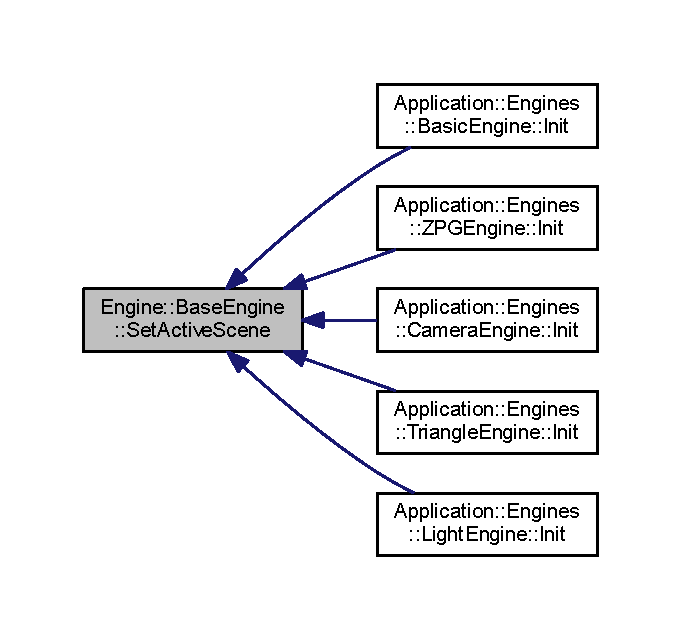
\includegraphics[width=327pt]{classEngine_1_1BaseEngine_afc82c6a00d5a9d4714740fc5eab5db86_icgraph}
\end{center}
\end{figure}
\mbox{\Hypertarget{classEngine_1_1BaseEngine_a525fdc7a1da7eecb514ad5763f06be79}\label{classEngine_1_1BaseEngine_a525fdc7a1da7eecb514ad5763f06be79}} 
\index{Application\+::\+Engines\+::\+Camera\+Engine@{Application\+::\+Engines\+::\+Camera\+Engine}!Start@{Start}}
\index{Start@{Start}!Application\+::\+Engines\+::\+Camera\+Engine@{Application\+::\+Engines\+::\+Camera\+Engine}}
\subsubsection{\texorpdfstring{Start()}{Start()}}
{\footnotesize\ttfamily void Engine\+::\+Base\+Engine\+::\+Start (\begin{DoxyParamCaption}{ }\end{DoxyParamCaption})\hspace{0.3cm}{\ttfamily [virtual]}, {\ttfamily [inherited]}}



Definition at line 126 of file Base\+Engine.\+cpp.



Referenced by main().


\begin{DoxyCode}
127 \{
128     system(\textcolor{stringliteral}{"cls"});
129     \mbox{\hyperlink{classEngine_1_1BaseEngine_aad3c237ca657b9f22f76fccf7fc7561f}{UpdateInternal}}();
130 \}
\end{DoxyCode}
Here is the caller graph for this function\+:
\nopagebreak
\begin{figure}[H]
\begin{center}
\leavevmode
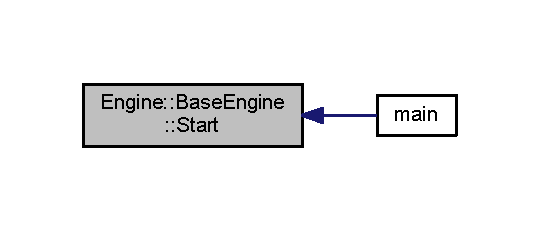
\includegraphics[width=259pt]{classEngine_1_1BaseEngine_a525fdc7a1da7eecb514ad5763f06be79_icgraph}
\end{center}
\end{figure}
\mbox{\Hypertarget{classApplication_1_1Engines_1_1CameraEngine_a48f10aa5b7d87545f5c04d69c37df665}\label{classApplication_1_1Engines_1_1CameraEngine_a48f10aa5b7d87545f5c04d69c37df665}} 
\index{Application\+::\+Engines\+::\+Camera\+Engine@{Application\+::\+Engines\+::\+Camera\+Engine}!Update@{Update}}
\index{Update@{Update}!Application\+::\+Engines\+::\+Camera\+Engine@{Application\+::\+Engines\+::\+Camera\+Engine}}
\subsubsection{\texorpdfstring{Update()}{Update()}\hspace{0.1cm}{\footnotesize\ttfamily [1/2]}}
{\footnotesize\ttfamily void Application\+::\+Engines\+::\+Camera\+Engine\+::\+Update (\begin{DoxyParamCaption}\item[{\+::\mbox{\hyperlink{classEngine_1_1Components_1_1Window}{Engine\+::\+Components\+::\+Window}} $\ast$}]{window }\end{DoxyParamCaption})\hspace{0.3cm}{\ttfamily [override]}}



Definition at line 75 of file Camera\+Engine.\+cpp.



References Engine\+::\+Components\+::\+Window\+::\+Height, and Engine\+::\+Components\+::\+Window\+::\+Width.


\begin{DoxyCode}
76 \{
77     \textcolor{keywordflow}{if} (\mbox{\hyperlink{classEngine_1_1BaseEngine_adb3dbc839da9d821e08b18d8a221698d}{ActiveScene}} != \textcolor{keyword}{nullptr} && \mbox{\hyperlink{classEngine_1_1BaseEngine_adb3dbc839da9d821e08b18d8a221698d}{ActiveScene}}->\mbox{\hyperlink{classEngine_1_1Components_1_1Scene_a23481feabaaa56bf5613765db03af4da}{Objects}} != \textcolor{keyword}{nullptr} && !
      \mbox{\hyperlink{classEngine_1_1BaseEngine_adb3dbc839da9d821e08b18d8a221698d}{ActiveScene}}->\mbox{\hyperlink{classEngine_1_1Components_1_1Scene_a23481feabaaa56bf5613765db03af4da}{Objects}}->empty())
78         \textcolor{keywordflow}{for} (\textcolor{keyword}{auto}& it : *\mbox{\hyperlink{classEngine_1_1BaseEngine_adb3dbc839da9d821e08b18d8a221698d}{ActiveScene}}->\mbox{\hyperlink{classEngine_1_1Components_1_1Scene_a23481feabaaa56bf5613765db03af4da}{Objects}})
79         \{
80             \textcolor{comment}{//auto \_fi = atan2(MouseY, MouseX);}
81             \textcolor{comment}{//auto \_psi = atan2(MouseX, MouseY);}
82             \textcolor{comment}{//auto \_fi = glm::radians(MouseX);}
83             \textcolor{comment}{//auto \_psi = glm::radians(MouseY);}
84             \textcolor{keyword}{auto} \_fi = (\mbox{\hyperlink{classEngine_1_1BaseEngine_a5fe085152ebe93346900407f6b41a034}{MouseX}} / window->\mbox{\hyperlink{classEngine_1_1Components_1_1Window_ad9cf40200634bff27dbc7ae9a841bb99}{Height}});
85             \textcolor{keyword}{auto} \_psi =(\mbox{\hyperlink{classEngine_1_1BaseEngine_a143c9c32dbbdc70bf1546ffe275bf384}{MouseY}} / window->\mbox{\hyperlink{classEngine_1_1Components_1_1Window_ad5f71bfbb06ff5452b63bddf4b0c20b1}{Width}});
86 
87             std::cout << \textcolor{stringliteral}{"FI:  "} << \_fi << \textcolor{stringliteral}{"\(\backslash\)nPSI: "} << \_psi << \textcolor{stringliteral}{"\(\backslash\)nObject: "} << it.first << std::endl;
88 
89             \mbox{\hyperlink{classEngine_1_1BaseEngine_adb3dbc839da9d821e08b18d8a221698d}{ActiveScene}}->\mbox{\hyperlink{classEngine_1_1Components_1_1Scene_aea98ff1ced88ee859878b504e9a2a362}{Cameras}}->First()->SetDirection(\textcolor{keyword}{new} glm::vec3(cos(\_fi), sin(\_fi),
       cos(\_psi)));
90 
91             \textcolor{keyword}{auto} \textcolor{keywordtype}{object} = it.second;
92             \textcolor{keywordtype}{object}->Draw();
93 
94             \textcolor{comment}{/*auto pm = glm::perspective(glm::radians(90.0f), 4.0f / 3.0f, 0.1f, 100.0f);}
95 \textcolor{comment}{            auto c = ActiveScene->Cameras->First()->Value;}
96 \textcolor{comment}{            Shaders->Get("vertex")->SendUniform(Programs->First(), "viewMatrix", c);}
97 \textcolor{comment}{            Shaders->Get("vertex")->SendUniform(Programs->First(), "projectionMatrix", &pm);*/}
98             \mbox{\hyperlink{classApplication_1_1Engines_1_1CameraEngine_a5298e9f5fa1a2984e21274c4524f771c}{angle}} += 0.1f;
99         \}
100 \}
\end{DoxyCode}
\mbox{\Hypertarget{classEngine_1_1BaseEngine_a01c23c2073f08939a660f3b7a866852c}\label{classEngine_1_1BaseEngine_a01c23c2073f08939a660f3b7a866852c}} 
\index{Application\+::\+Engines\+::\+Camera\+Engine@{Application\+::\+Engines\+::\+Camera\+Engine}!Update@{Update}}
\index{Update@{Update}!Application\+::\+Engines\+::\+Camera\+Engine@{Application\+::\+Engines\+::\+Camera\+Engine}}
\subsubsection{\texorpdfstring{Update()}{Update()}\hspace{0.1cm}{\footnotesize\ttfamily [2/2]}}
{\footnotesize\ttfamily void Engine\+::\+Base\+Engine\+::\+Update (\begin{DoxyParamCaption}\item[{\mbox{\hyperlink{classEngine_1_1Components_1_1Window}{Components\+::\+Window}} $\ast$}]{window }\end{DoxyParamCaption})\hspace{0.3cm}{\ttfamily [virtual]}, {\ttfamily [inherited]}}



Definition at line 112 of file Base\+Engine.\+cpp.


\begin{DoxyCode}
113 \{
114 \}
\end{DoxyCode}
\mbox{\Hypertarget{classEngine_1_1BaseEngine_aace6be2a42d12b64fbd35f1acdb08408}\label{classEngine_1_1BaseEngine_aace6be2a42d12b64fbd35f1acdb08408}} 
\index{Application\+::\+Engines\+::\+Camera\+Engine@{Application\+::\+Engines\+::\+Camera\+Engine}!Update\+Begin@{Update\+Begin}}
\index{Update\+Begin@{Update\+Begin}!Application\+::\+Engines\+::\+Camera\+Engine@{Application\+::\+Engines\+::\+Camera\+Engine}}
\subsubsection{\texorpdfstring{Update\+Begin()}{UpdateBegin()}}
{\footnotesize\ttfamily void Engine\+::\+Base\+Engine\+::\+Update\+Begin (\begin{DoxyParamCaption}\item[{\mbox{\hyperlink{classEngine_1_1Components_1_1Window}{Components\+::\+Window}} $\ast$}]{window }\end{DoxyParamCaption})\hspace{0.3cm}{\ttfamily [virtual]}, {\ttfamily [inherited]}}



Definition at line 57 of file Base\+Engine.\+cpp.



References Engine\+::\+Components\+::\+Window\+::\+Get().


\begin{DoxyCode}
58 \{
59     \textcolor{comment}{// Scene}
60     \mbox{\hyperlink{classEngine_1_1BaseEngine_adb3dbc839da9d821e08b18d8a221698d}{ActiveScene}}->\mbox{\hyperlink{classEngine_1_1Components_1_1Scene_af18bd334fe66952b8d79b8e9e99ab2d8}{BeginLoad}}(\textcolor{keyword}{this});
61 
62     \textcolor{comment}{// Buffers}
63     glEnable(GL\_DEPTH\_TEST);
64     glDepthFunc(GL\_LESS);
65     glClear(GL\_COLOR\_BUFFER\_BIT | GL\_DEPTH\_BUFFER\_BIT);
66 
67     \textcolor{comment}{// Input}
68     \textcolor{keywordtype}{short} mouseKeysActive = 0;
69     glfwGetCursorPos(window->Get(), &\mbox{\hyperlink{classEngine_1_1BaseEngine_a5fe085152ebe93346900407f6b41a034}{MouseX}}, &\mbox{\hyperlink{classEngine_1_1BaseEngine_a143c9c32dbbdc70bf1546ffe275bf384}{MouseY}});
70     \textcolor{keywordflow}{for}(\textcolor{keywordtype}{short} i = 0; i < 8; i++)
71     \{
72         \textcolor{keyword}{const} \textcolor{keywordtype}{int} state = glfwGetMouseButton(window->Get(), i);
73         \textcolor{keyword}{auto} value = \mbox{\hyperlink{classEngine_1_1BaseEngine_a3ee2bdddb66d45b8c808ffd937ba9c50}{MouseKeys}}[i];
74         \textcolor{comment}{// flip state}
75         \textcolor{keywordflow}{if} (state == GLFW\_PRESS && !value)
76             \mbox{\hyperlink{classEngine_1_1BaseEngine_a3ee2bdddb66d45b8c808ffd937ba9c50}{MouseKeys}}.\mbox{\hyperlink{classGeneric_1_1Dictionary_ae7cb006f801b21c172e8fbac8794fa99}{Add}}(i, \textcolor{keyword}{true});
77         \textcolor{keywordflow}{else} \textcolor{keywordflow}{if} (state == GLFW\_RELEASE && value)
78             \mbox{\hyperlink{classEngine_1_1BaseEngine_a3ee2bdddb66d45b8c808ffd937ba9c50}{MouseKeys}}.\mbox{\hyperlink{classGeneric_1_1Dictionary_ae7cb006f801b21c172e8fbac8794fa99}{Add}}(i, \textcolor{keyword}{false});
79         \textcolor{keywordflow}{if} (\mbox{\hyperlink{classEngine_1_1BaseEngine_a3ee2bdddb66d45b8c808ffd937ba9c50}{MouseKeys}}[i])
80             mouseKeysActive++;
81     \}
82     \textcolor{keywordtype}{short} keysActive = 0;
83     SetConsoleCursorPosition(GetStdHandle(STD\_OUTPUT\_HANDLE), \{ 40, keysActive \});
84     fprintf(\mbox{\hyperlink{classEngine_1_1BaseEngine_a26fd54a1ee2733f9c654af5afcfa96cf}{\_errorStream}}, \textcolor{stringliteral}{"                           "});
85     \textcolor{keywordflow}{for} (\textcolor{keywordtype}{short} i = 1; i < 512; i++)
86     \{
87         \textcolor{keyword}{const} \textcolor{keywordtype}{int} state = glfwGetKey(window->Get(), i);
88         \textcolor{keyword}{auto} value = \mbox{\hyperlink{classEngine_1_1BaseEngine_a65321a97e83f0a6ee90df3efac2d3307}{Keys}}[i];
89         \textcolor{comment}{// flip state}
90         \textcolor{keywordflow}{if} (state == GLFW\_PRESS && !value)
91             \mbox{\hyperlink{classEngine_1_1BaseEngine_a65321a97e83f0a6ee90df3efac2d3307}{Keys}}.\mbox{\hyperlink{classGeneric_1_1Dictionary_ae7cb006f801b21c172e8fbac8794fa99}{Add}}(i, \textcolor{keyword}{true});
92         \textcolor{keywordflow}{else} \textcolor{keywordflow}{if} (state == GLFW\_RELEASE && value)
93             \mbox{\hyperlink{classEngine_1_1BaseEngine_a65321a97e83f0a6ee90df3efac2d3307}{Keys}}.\mbox{\hyperlink{classGeneric_1_1Dictionary_ae7cb006f801b21c172e8fbac8794fa99}{Add}}(i, \textcolor{keyword}{false});
94         \textcolor{keywordflow}{if} (\mbox{\hyperlink{classEngine_1_1BaseEngine_a65321a97e83f0a6ee90df3efac2d3307}{Keys}}[i])
95             keysActive++;
96     \}
97     \textcolor{keywordtype}{bool} handleKeys = \textcolor{keyword}{true},
98          handleMouse = \textcolor{keyword}{true};
99     \textcolor{keywordflow}{for} (\textcolor{keyword}{auto} handler : *\mbox{\hyperlink{classEngine_1_1BaseEngine_a134fa082c5a64d62b76ddf926647e7cc}{InputHandlers}})
100     \{
101         \textcolor{keywordflow}{if}(handleKeys)
102             handleKeys = handler->HandleKeys(\textcolor{keyword}{this}, window, \mbox{\hyperlink{classEngine_1_1BaseEngine_adb3dbc839da9d821e08b18d8a221698d}{ActiveScene}}, 
      \mbox{\hyperlink{classEngine_1_1BaseEngine_a65321a97e83f0a6ee90df3efac2d3307}{Keys}}, keysActive);
103         \textcolor{keywordflow}{if}(handleMouse)
104             handleMouse = handler->HandleMouse(\textcolor{keyword}{this}, window, \mbox{\hyperlink{classEngine_1_1BaseEngine_adb3dbc839da9d821e08b18d8a221698d}{ActiveScene}}, 
      \mbox{\hyperlink{classEngine_1_1BaseEngine_a5fe085152ebe93346900407f6b41a034}{MouseX}}, \mbox{\hyperlink{classEngine_1_1BaseEngine_a143c9c32dbbdc70bf1546ffe275bf384}{MouseY}}, \mbox{\hyperlink{classEngine_1_1BaseEngine_a3ee2bdddb66d45b8c808ffd937ba9c50}{MouseKeys}}, mouseKeysActive);
105         \textcolor{keywordflow}{if}(!handleKeys && !handleMouse)
106             \textcolor{keywordflow}{break};
107     \}
108 
109     SetConsoleCursorPosition(GetStdHandle(STD\_OUTPUT\_HANDLE), \{ 0,0 \});
110 \}
\end{DoxyCode}
Here is the call graph for this function\+:
\nopagebreak
\begin{figure}[H]
\begin{center}
\leavevmode
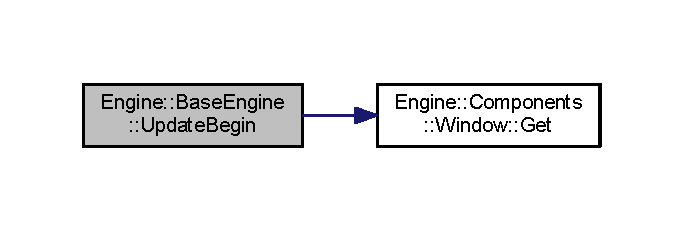
\includegraphics[width=328pt]{classEngine_1_1BaseEngine_aace6be2a42d12b64fbd35f1acdb08408_cgraph}
\end{center}
\end{figure}
\mbox{\Hypertarget{classEngine_1_1BaseEngine_a7c07c98e583df042a0eb01e0ddec85a1}\label{classEngine_1_1BaseEngine_a7c07c98e583df042a0eb01e0ddec85a1}} 
\index{Application\+::\+Engines\+::\+Camera\+Engine@{Application\+::\+Engines\+::\+Camera\+Engine}!Update\+End@{Update\+End}}
\index{Update\+End@{Update\+End}!Application\+::\+Engines\+::\+Camera\+Engine@{Application\+::\+Engines\+::\+Camera\+Engine}}
\subsubsection{\texorpdfstring{Update\+End()}{UpdateEnd()}}
{\footnotesize\ttfamily void Engine\+::\+Base\+Engine\+::\+Update\+End (\begin{DoxyParamCaption}\item[{\mbox{\hyperlink{classEngine_1_1Components_1_1Window}{Components\+::\+Window}} $\ast$}]{window }\end{DoxyParamCaption})\hspace{0.3cm}{\ttfamily [virtual]}, {\ttfamily [inherited]}}



Definition at line 116 of file Base\+Engine.\+cpp.



References Engine\+::\+Components\+::\+Window\+::\+Get().


\begin{DoxyCode}
117 \{
118     \textcolor{comment}{// update other events like input handling}
119     glfwPollEvents();
120     \textcolor{comment}{// put the stuff we’ve been drawing onto the display}
121     glfwSwapBuffers(window->Get());
122 
123     \mbox{\hyperlink{classEngine_1_1BaseEngine_adb3dbc839da9d821e08b18d8a221698d}{ActiveScene}}->\mbox{\hyperlink{classEngine_1_1Components_1_1Scene_abd8fcdcac52dbce6a0a18de3860ab087}{FrameUpdate}}(\textcolor{keyword}{this});
124 \}
\end{DoxyCode}
Here is the call graph for this function\+:
\nopagebreak
\begin{figure}[H]
\begin{center}
\leavevmode
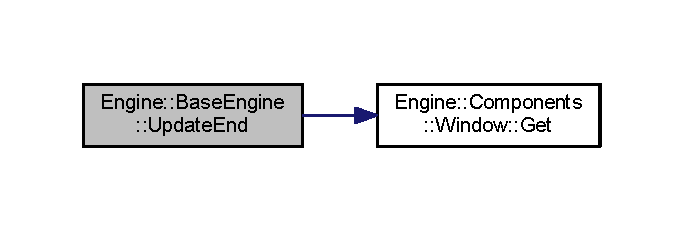
\includegraphics[width=328pt]{classEngine_1_1BaseEngine_a7c07c98e583df042a0eb01e0ddec85a1_cgraph}
\end{center}
\end{figure}


\subsection{Member Data Documentation}
\mbox{\Hypertarget{classEngine_1_1BaseEngine_adb3dbc839da9d821e08b18d8a221698d}\label{classEngine_1_1BaseEngine_adb3dbc839da9d821e08b18d8a221698d}} 
\index{Application\+::\+Engines\+::\+Camera\+Engine@{Application\+::\+Engines\+::\+Camera\+Engine}!Active\+Scene@{Active\+Scene}}
\index{Active\+Scene@{Active\+Scene}!Application\+::\+Engines\+::\+Camera\+Engine@{Application\+::\+Engines\+::\+Camera\+Engine}}
\subsubsection{\texorpdfstring{Active\+Scene}{ActiveScene}}
{\footnotesize\ttfamily Components\+::\+Scene$\ast$ Engine\+::\+Base\+Engine\+::\+Active\+Scene\hspace{0.3cm}{\ttfamily [inherited]}}



Definition at line 34 of file Base\+Engine.\+h.



Referenced by Engine\+::\+Base\+Engine\+::\+Base\+Engine(), Init(), and Application\+::\+Engines\+::\+Light\+Engine\+::\+Init().

\mbox{\Hypertarget{classApplication_1_1Engines_1_1CameraEngine_a5298e9f5fa1a2984e21274c4524f771c}\label{classApplication_1_1Engines_1_1CameraEngine_a5298e9f5fa1a2984e21274c4524f771c}} 
\index{Application\+::\+Engines\+::\+Camera\+Engine@{Application\+::\+Engines\+::\+Camera\+Engine}!angle@{angle}}
\index{angle@{angle}!Application\+::\+Engines\+::\+Camera\+Engine@{Application\+::\+Engines\+::\+Camera\+Engine}}
\subsubsection{\texorpdfstring{angle}{angle}}
{\footnotesize\ttfamily float Application\+::\+Engines\+::\+Camera\+Engine\+::angle\hspace{0.3cm}{\ttfamily [private]}}



Definition at line 15 of file Camera\+Engine.\+h.



Referenced by Init().

\mbox{\Hypertarget{classEngine_1_1BaseEngine_a134fa082c5a64d62b76ddf926647e7cc}\label{classEngine_1_1BaseEngine_a134fa082c5a64d62b76ddf926647e7cc}} 
\index{Application\+::\+Engines\+::\+Camera\+Engine@{Application\+::\+Engines\+::\+Camera\+Engine}!Input\+Handlers@{Input\+Handlers}}
\index{Input\+Handlers@{Input\+Handlers}!Application\+::\+Engines\+::\+Camera\+Engine@{Application\+::\+Engines\+::\+Camera\+Engine}}
\subsubsection{\texorpdfstring{Input\+Handlers}{InputHandlers}}
{\footnotesize\ttfamily \mbox{\hyperlink{classGeneric_1_1Collection}{Generic\+::\+Collection}}$<$Components\+::\+I\+Input\+Handler$\ast$$>$$\ast$ Engine\+::\+Base\+Engine\+::\+Input\+Handlers\hspace{0.3cm}{\ttfamily [inherited]}}



Definition at line 31 of file Base\+Engine.\+h.



Referenced by Engine\+::\+Base\+Engine\+::\+Base\+Engine(), and Application\+::\+Engines\+::\+Light\+Engine\+::\+Init().

\mbox{\Hypertarget{classEngine_1_1BaseEngine_a65321a97e83f0a6ee90df3efac2d3307}\label{classEngine_1_1BaseEngine_a65321a97e83f0a6ee90df3efac2d3307}} 
\index{Application\+::\+Engines\+::\+Camera\+Engine@{Application\+::\+Engines\+::\+Camera\+Engine}!Keys@{Keys}}
\index{Keys@{Keys}!Application\+::\+Engines\+::\+Camera\+Engine@{Application\+::\+Engines\+::\+Camera\+Engine}}
\subsubsection{\texorpdfstring{Keys}{Keys}}
{\footnotesize\ttfamily \mbox{\hyperlink{classGeneric_1_1Dictionary}{Generic\+::\+Dictionary}}$<$short, bool$>$ Engine\+::\+Base\+Engine\+::\+Keys\hspace{0.3cm}{\ttfamily [inherited]}}



Definition at line 32 of file Base\+Engine.\+h.



Referenced by Engine\+::\+Base\+Engine\+::\+Base\+Engine().

\mbox{\Hypertarget{classApplication_1_1Engines_1_1CameraEngine_a2c5eb2ee7aa78a335df64d77242fb21c}\label{classApplication_1_1Engines_1_1CameraEngine_a2c5eb2ee7aa78a335df64d77242fb21c}} 
\index{Application\+::\+Engines\+::\+Camera\+Engine@{Application\+::\+Engines\+::\+Camera\+Engine}!M@{M}}
\index{M@{M}!Application\+::\+Engines\+::\+Camera\+Engine@{Application\+::\+Engines\+::\+Camera\+Engine}}
\subsubsection{\texorpdfstring{M}{M}}
{\footnotesize\ttfamily glm\+::mat4 Application\+::\+Engines\+::\+Camera\+Engine\+::M\hspace{0.3cm}{\ttfamily [private]}}



Definition at line 14 of file Camera\+Engine.\+h.



Referenced by Init().

\mbox{\Hypertarget{classEngine_1_1BaseEngine_a3ee2bdddb66d45b8c808ffd937ba9c50}\label{classEngine_1_1BaseEngine_a3ee2bdddb66d45b8c808ffd937ba9c50}} 
\index{Application\+::\+Engines\+::\+Camera\+Engine@{Application\+::\+Engines\+::\+Camera\+Engine}!Mouse\+Keys@{Mouse\+Keys}}
\index{Mouse\+Keys@{Mouse\+Keys}!Application\+::\+Engines\+::\+Camera\+Engine@{Application\+::\+Engines\+::\+Camera\+Engine}}
\subsubsection{\texorpdfstring{Mouse\+Keys}{MouseKeys}}
{\footnotesize\ttfamily \mbox{\hyperlink{classGeneric_1_1Dictionary}{Generic\+::\+Dictionary}}$<$short, bool$>$ Engine\+::\+Base\+Engine\+::\+Mouse\+Keys\hspace{0.3cm}{\ttfamily [inherited]}}



Definition at line 33 of file Base\+Engine.\+h.



Referenced by Engine\+::\+Base\+Engine\+::\+Base\+Engine().

\mbox{\Hypertarget{classEngine_1_1BaseEngine_a5fe085152ebe93346900407f6b41a034}\label{classEngine_1_1BaseEngine_a5fe085152ebe93346900407f6b41a034}} 
\index{Application\+::\+Engines\+::\+Camera\+Engine@{Application\+::\+Engines\+::\+Camera\+Engine}!MouseX@{MouseX}}
\index{MouseX@{MouseX}!Application\+::\+Engines\+::\+Camera\+Engine@{Application\+::\+Engines\+::\+Camera\+Engine}}
\subsubsection{\texorpdfstring{MouseX}{MouseX}}
{\footnotesize\ttfamily double Engine\+::\+Base\+Engine\+::\+MouseX\hspace{0.3cm}{\ttfamily [inherited]}}



Definition at line 35 of file Base\+Engine.\+h.

\mbox{\Hypertarget{classEngine_1_1BaseEngine_a143c9c32dbbdc70bf1546ffe275bf384}\label{classEngine_1_1BaseEngine_a143c9c32dbbdc70bf1546ffe275bf384}} 
\index{Application\+::\+Engines\+::\+Camera\+Engine@{Application\+::\+Engines\+::\+Camera\+Engine}!MouseY@{MouseY}}
\index{MouseY@{MouseY}!Application\+::\+Engines\+::\+Camera\+Engine@{Application\+::\+Engines\+::\+Camera\+Engine}}
\subsubsection{\texorpdfstring{MouseY}{MouseY}}
{\footnotesize\ttfamily double Engine\+::\+Base\+Engine\+::\+MouseY\hspace{0.3cm}{\ttfamily [inherited]}}



Definition at line 36 of file Base\+Engine.\+h.

\mbox{\Hypertarget{classEngine_1_1BaseEngine_ae0f86360ea3a384caefe443dd8f88601}\label{classEngine_1_1BaseEngine_ae0f86360ea3a384caefe443dd8f88601}} 
\index{Application\+::\+Engines\+::\+Camera\+Engine@{Application\+::\+Engines\+::\+Camera\+Engine}!Programs@{Programs}}
\index{Programs@{Programs}!Application\+::\+Engines\+::\+Camera\+Engine@{Application\+::\+Engines\+::\+Camera\+Engine}}
\subsubsection{\texorpdfstring{Programs}{Programs}}
{\footnotesize\ttfamily \mbox{\hyperlink{classGeneric_1_1Dictionary}{Generic\+::\+Dictionary}}$<$std\+::string, Components\+::\+Graphics\+::\+Program$\ast$$>$$\ast$ Engine\+::\+Base\+Engine\+::\+Programs\hspace{0.3cm}{\ttfamily [inherited]}}



Definition at line 28 of file Base\+Engine.\+h.



Referenced by Engine\+::\+Base\+Engine\+::\+Base\+Engine(), Application\+::\+Input\+::\+Handlers\+::\+Camera\+Input\+Handler\+::\+Handle\+Mouse(), Application\+::\+Engines\+::\+Triangle\+Engine\+::\+Init(), Application\+::\+Engines\+::\+Basic\+Engine\+::\+Init(), Init(), Application\+::\+Engines\+::\+Z\+P\+G\+Engine\+::\+Init(), Application\+::\+Engines\+::\+Light\+Engine\+::\+Init(), Application\+::\+Scenes\+::\+Triangle\+Scene\+::\+Load(), and Application\+::\+Scenes\+::\+Sphere\+Scene\+::\+Load().

\mbox{\Hypertarget{classEngine_1_1BaseEngine_afd02af3c2fbe9bb734db014dec06585a}\label{classEngine_1_1BaseEngine_afd02af3c2fbe9bb734db014dec06585a}} 
\index{Application\+::\+Engines\+::\+Camera\+Engine@{Application\+::\+Engines\+::\+Camera\+Engine}!Scenes@{Scenes}}
\index{Scenes@{Scenes}!Application\+::\+Engines\+::\+Camera\+Engine@{Application\+::\+Engines\+::\+Camera\+Engine}}
\subsubsection{\texorpdfstring{Scenes}{Scenes}}
{\footnotesize\ttfamily \mbox{\hyperlink{classGeneric_1_1Dictionary}{Generic\+::\+Dictionary}}$<$std\+::string, Components\+::\+Scene$\ast$$>$$\ast$ Engine\+::\+Base\+Engine\+::\+Scenes\hspace{0.3cm}{\ttfamily [inherited]}}



Definition at line 30 of file Base\+Engine.\+h.



Referenced by Engine\+::\+Base\+Engine\+::\+Base\+Engine(), Application\+::\+Engines\+::\+Z\+P\+G\+Engine\+::\+Init(), Init(), Application\+::\+Engines\+::\+Basic\+Engine\+::\+Init(), Application\+::\+Engines\+::\+Triangle\+Engine\+::\+Init(), and Application\+::\+Engines\+::\+Light\+Engine\+::\+Init().

\mbox{\Hypertarget{classEngine_1_1BaseEngine_a2582dee3f73da82bb422b43317b85e3b}\label{classEngine_1_1BaseEngine_a2582dee3f73da82bb422b43317b85e3b}} 
\index{Application\+::\+Engines\+::\+Camera\+Engine@{Application\+::\+Engines\+::\+Camera\+Engine}!Shaders@{Shaders}}
\index{Shaders@{Shaders}!Application\+::\+Engines\+::\+Camera\+Engine@{Application\+::\+Engines\+::\+Camera\+Engine}}
\subsubsection{\texorpdfstring{Shaders}{Shaders}}
{\footnotesize\ttfamily \mbox{\hyperlink{classGeneric_1_1Dictionary}{Generic\+::\+Dictionary}}$<$std\+::string, Components\+::\+Graphics\+::\+Shader$\ast$$>$$\ast$ Engine\+::\+Base\+Engine\+::\+Shaders\hspace{0.3cm}{\ttfamily [inherited]}}



Definition at line 29 of file Base\+Engine.\+h.



Referenced by Engine\+::\+Base\+Engine\+::\+Base\+Engine(), Application\+::\+Input\+::\+Handlers\+::\+Camera\+Input\+Handler\+::\+Handle\+Mouse(), Init(), Application\+::\+Engines\+::\+Basic\+Engine\+::\+Init(), Application\+::\+Engines\+::\+Z\+P\+G\+Engine\+::\+Init(), Application\+::\+Engines\+::\+Triangle\+Engine\+::\+Init(), and Application\+::\+Engines\+::\+Light\+Engine\+::\+Init().

\mbox{\Hypertarget{classEngine_1_1BaseEngine_a4a1a4c4dae052e66ecc4f326eeed4d33}\label{classEngine_1_1BaseEngine_a4a1a4c4dae052e66ecc4f326eeed4d33}} 
\index{Application\+::\+Engines\+::\+Camera\+Engine@{Application\+::\+Engines\+::\+Camera\+Engine}!Windows@{Windows}}
\index{Windows@{Windows}!Application\+::\+Engines\+::\+Camera\+Engine@{Application\+::\+Engines\+::\+Camera\+Engine}}
\subsubsection{\texorpdfstring{Windows}{Windows}}
{\footnotesize\ttfamily \mbox{\hyperlink{classGeneric_1_1Dictionary}{Generic\+::\+Dictionary}}$<$std\+::string, Components\+::\+Window$\ast$$>$$\ast$ Engine\+::\+Base\+Engine\+::\+Windows\hspace{0.3cm}{\ttfamily [inherited]}}



Definition at line 27 of file Base\+Engine.\+h.



Referenced by Engine\+::\+Base\+Engine\+::\+Base\+Engine(), Application\+::\+Engines\+::\+Z\+P\+G\+Engine\+::\+Init(), Init(), Application\+::\+Engines\+::\+Basic\+Engine\+::\+Init(), Application\+::\+Engines\+::\+Triangle\+Engine\+::\+Init(), and Application\+::\+Engines\+::\+Light\+Engine\+::\+Init().



The documentation for this class was generated from the following files\+:\begin{DoxyCompactItemize}
\item 
Z\+P\+G/\mbox{\hyperlink{CameraEngine_8h}{Camera\+Engine.\+h}}\item 
Z\+P\+G/\mbox{\hyperlink{CameraEngine_8cpp}{Camera\+Engine.\+cpp}}\end{DoxyCompactItemize}

\hypertarget{classApplication_1_1Engines_1_1LightEngine}{}\section{Application\+:\+:Engines\+:\+:Light\+Engine Class Reference}
\label{classApplication_1_1Engines_1_1LightEngine}\index{Application\+::\+Engines\+::\+Light\+Engine@{Application\+::\+Engines\+::\+Light\+Engine}}


{\ttfamily \#include $<$Ligt\+Engine.\+h$>$}



Inheritance diagram for Application\+:\+:Engines\+:\+:Light\+Engine\+:
\nopagebreak
\begin{figure}[H]
\begin{center}
\leavevmode
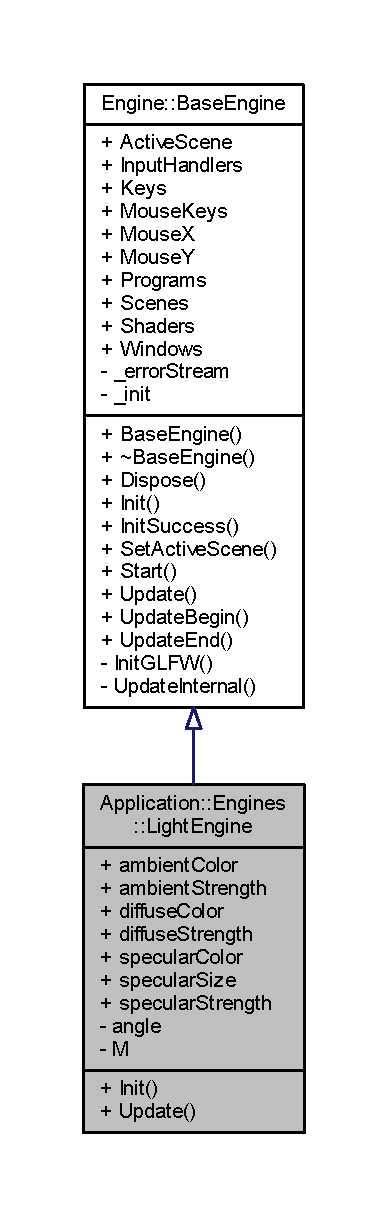
\includegraphics[height=550pt]{classApplication_1_1Engines_1_1LightEngine__inherit__graph}
\end{center}
\end{figure}


Collaboration diagram for Application\+:\+:Engines\+:\+:Light\+Engine\+:
\nopagebreak
\begin{figure}[H]
\begin{center}
\leavevmode
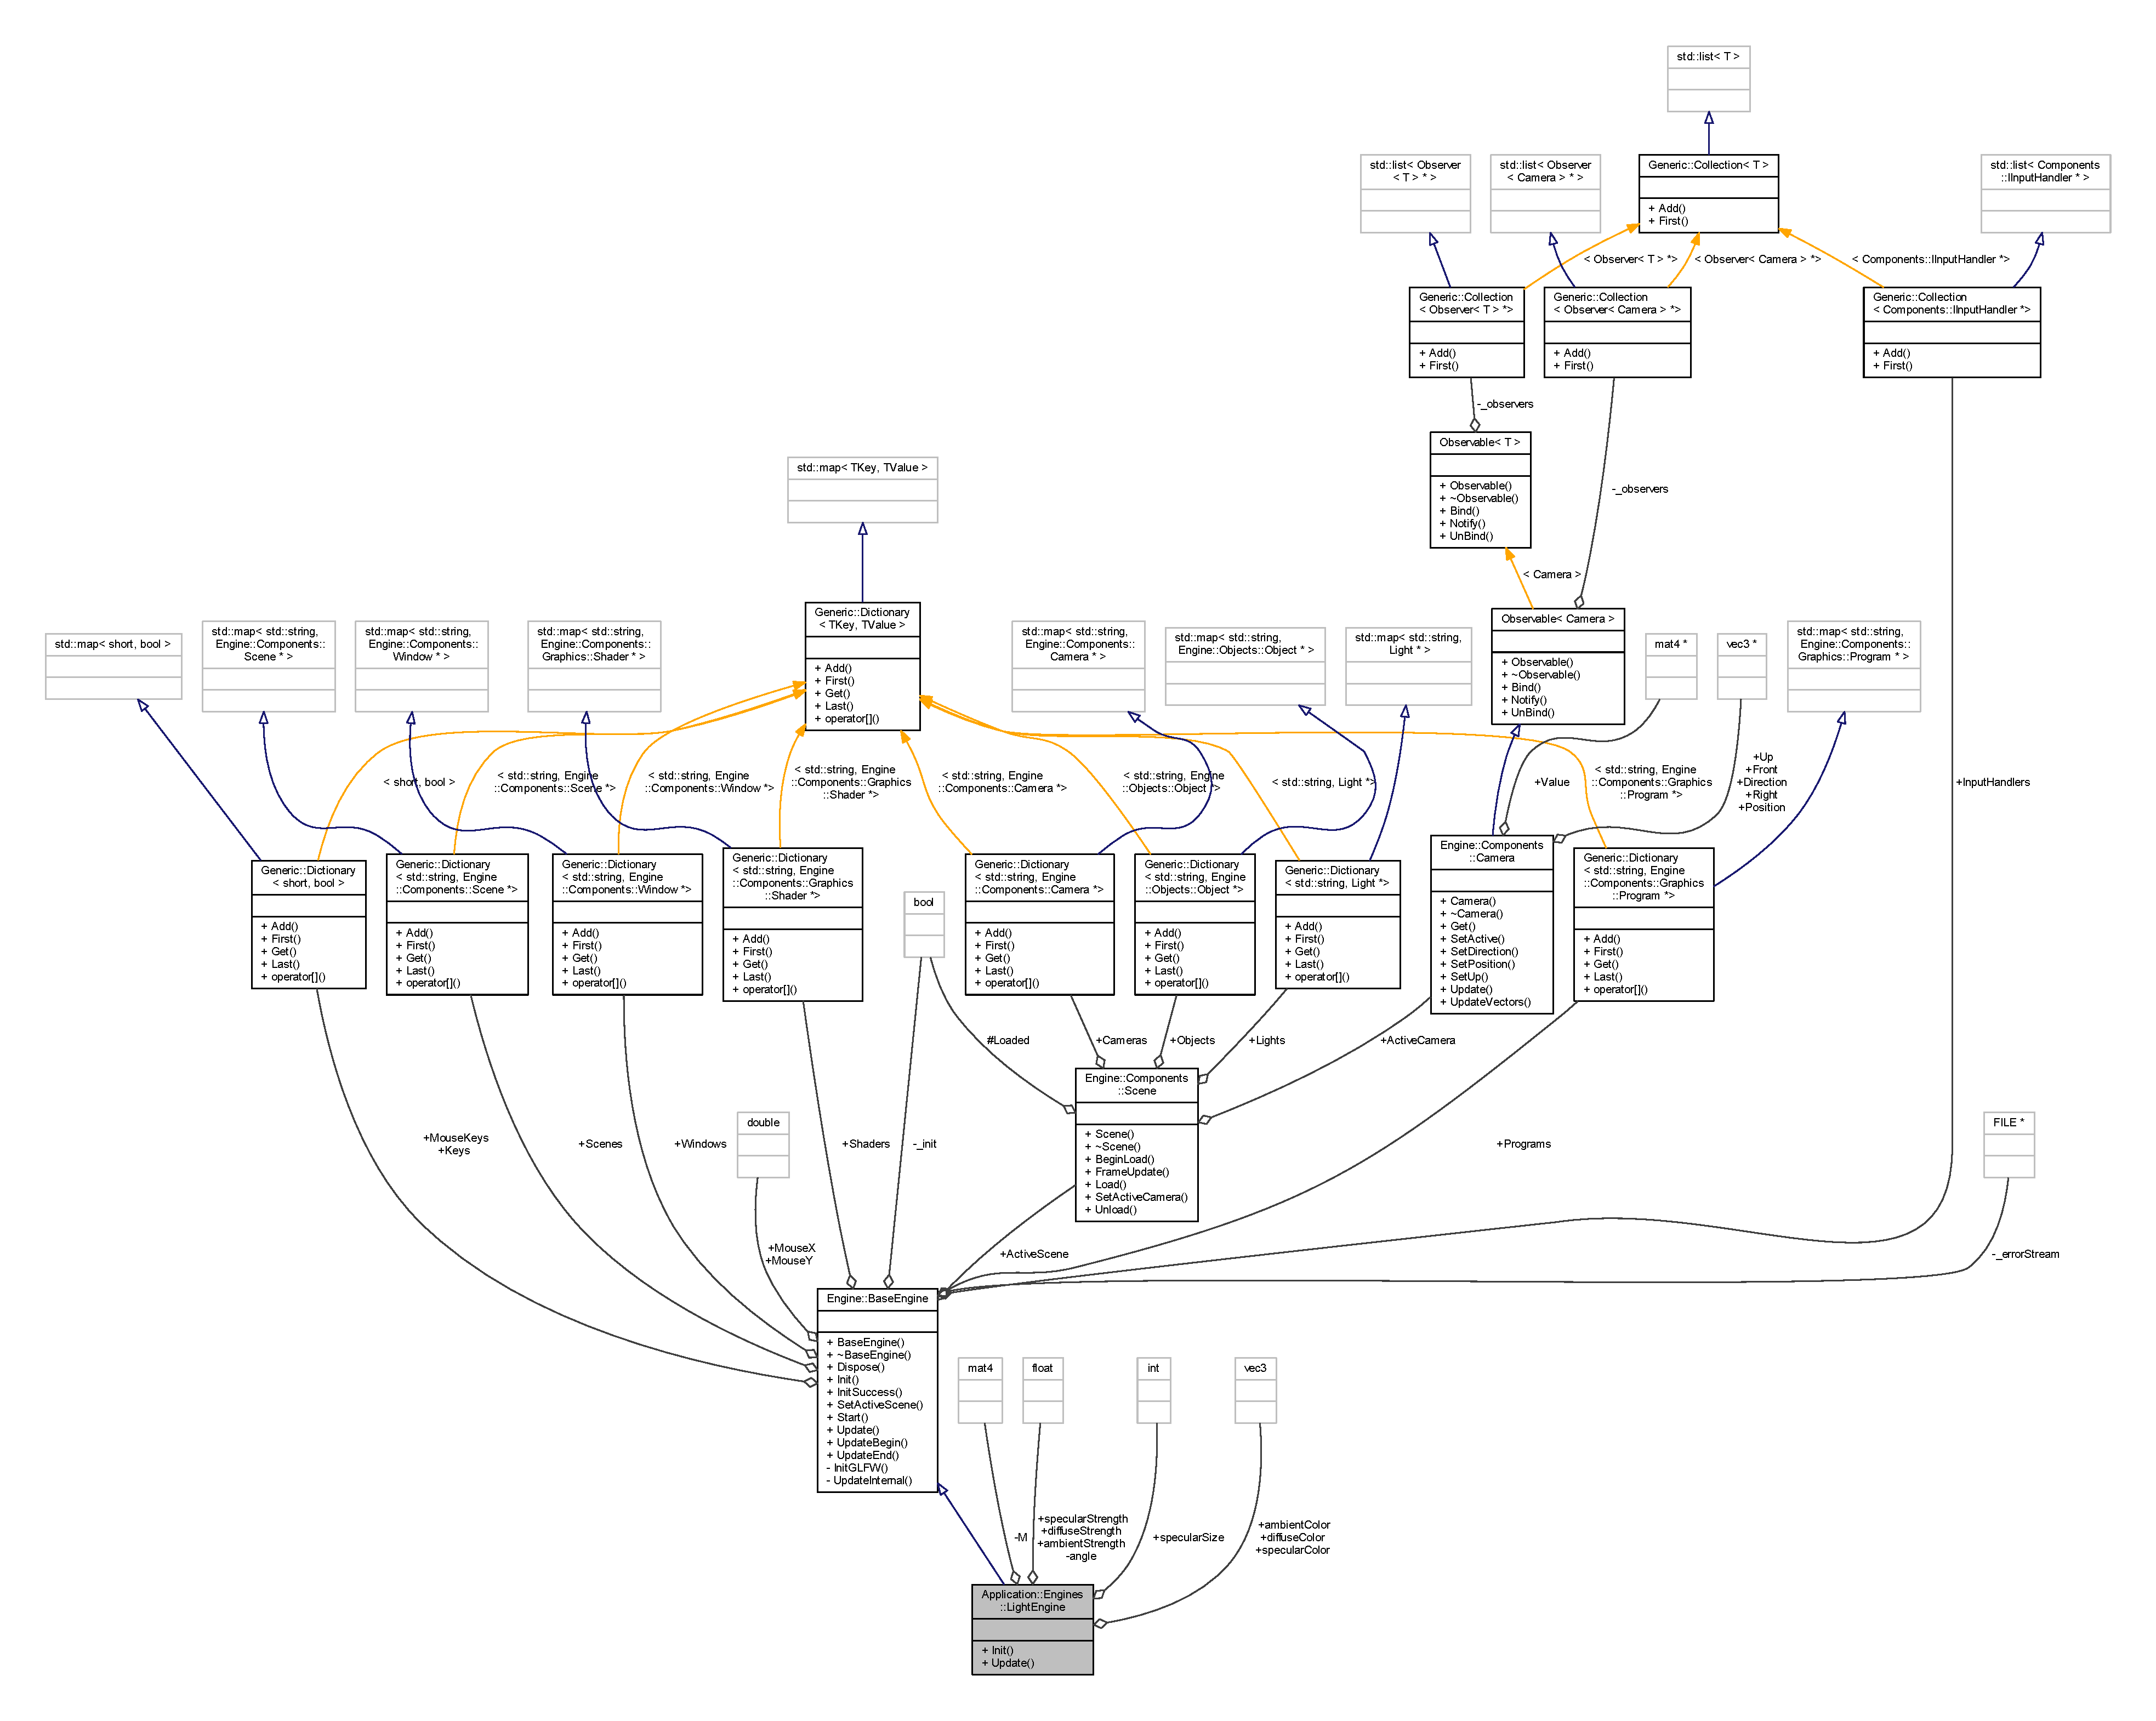
\includegraphics[width=350pt]{classApplication_1_1Engines_1_1LightEngine__coll__graph}
\end{center}
\end{figure}
\subsection*{Public Member Functions}
\begin{DoxyCompactItemize}
\item 
\mbox{\hyperlink{classEngine_1_1BaseEngine_ad838c97afe1790cb35527f0b58e81e6b}{Base\+Engine}} $\ast$ \mbox{\hyperlink{classEngine_1_1BaseEngine_acd5cd5d2189d24e038b23477b7dce405}{Dispose}} ()
\item 
\mbox{\hyperlink{classApplication_1_1Engines_1_1LightEngine}{Light\+Engine}} $\ast$ \mbox{\hyperlink{classApplication_1_1Engines_1_1LightEngine_ad992d8a300f099c247d7ba8dc38883ea}{Init}} (std\+::\+F\+I\+LE $\ast$error\+Stream=stderr) override
\item 
bool \mbox{\hyperlink{classEngine_1_1BaseEngine_a7a1c9b833049b3eb61194cab113dfe89}{Init\+Success}} ()
\item 
virtual void \mbox{\hyperlink{classEngine_1_1BaseEngine_afc82c6a00d5a9d4714740fc5eab5db86}{Set\+Active\+Scene}} (Components\+::\+Scene $\ast$scene=nullptr)
\item 
virtual void \mbox{\hyperlink{classEngine_1_1BaseEngine_a525fdc7a1da7eecb514ad5763f06be79}{Start}} ()
\item 
void \mbox{\hyperlink{classApplication_1_1Engines_1_1LightEngine_a18575df6f8742099ae543e3b23508ee9}{Update}} (\+::\mbox{\hyperlink{classEngine_1_1Components_1_1Window}{Engine\+::\+Components\+::\+Window}} $\ast$window) override
\item 
virtual void \mbox{\hyperlink{classEngine_1_1BaseEngine_a01c23c2073f08939a660f3b7a866852c}{Update}} (Components\+::\+Window $\ast$window)
\item 
virtual void \mbox{\hyperlink{classEngine_1_1BaseEngine_aace6be2a42d12b64fbd35f1acdb08408}{Update\+Begin}} (Components\+::\+Window $\ast$window)
\item 
virtual void \mbox{\hyperlink{classEngine_1_1BaseEngine_a7c07c98e583df042a0eb01e0ddec85a1}{Update\+End}} (Components\+::\+Window $\ast$window)
\end{DoxyCompactItemize}
\subsection*{Public Attributes}
\begin{DoxyCompactItemize}
\item 
Components\+::\+Scene $\ast$ \mbox{\hyperlink{classEngine_1_1BaseEngine_adb3dbc839da9d821e08b18d8a221698d}{Active\+Scene}}
\item 
glm\+::vec3 \mbox{\hyperlink{classApplication_1_1Engines_1_1LightEngine_ab22b7d03d1c3cd19214474fb56bdd2ee}{ambient\+Color}}
\item 
float \mbox{\hyperlink{classApplication_1_1Engines_1_1LightEngine_af97d743158c0e55c754b455e7066e6b0}{ambient\+Strength}}
\item 
glm\+::vec3 \mbox{\hyperlink{classApplication_1_1Engines_1_1LightEngine_a2247de4ba43b8d0e159ab90edd581363}{diffuse\+Color}}
\item 
float \mbox{\hyperlink{classApplication_1_1Engines_1_1LightEngine_ab2f3fb68d22dd1e6386833f4790a8eb6}{diffuse\+Strength}}
\item 
\mbox{\hyperlink{classGeneric_1_1Collection}{Generic\+::\+Collection}}$<$ Components\+::\+I\+Input\+Handler $\ast$ $>$ $\ast$ \mbox{\hyperlink{classEngine_1_1BaseEngine_a134fa082c5a64d62b76ddf926647e7cc}{Input\+Handlers}}
\item 
\mbox{\hyperlink{classGeneric_1_1Dictionary}{Generic\+::\+Dictionary}}$<$ short, bool $>$ \mbox{\hyperlink{classEngine_1_1BaseEngine_a65321a97e83f0a6ee90df3efac2d3307}{Keys}}
\item 
\mbox{\hyperlink{classGeneric_1_1Dictionary}{Generic\+::\+Dictionary}}$<$ short, bool $>$ \mbox{\hyperlink{classEngine_1_1BaseEngine_a3ee2bdddb66d45b8c808ffd937ba9c50}{Mouse\+Keys}}
\item 
double \mbox{\hyperlink{classEngine_1_1BaseEngine_a5fe085152ebe93346900407f6b41a034}{MouseX}}
\item 
double \mbox{\hyperlink{classEngine_1_1BaseEngine_a143c9c32dbbdc70bf1546ffe275bf384}{MouseY}}
\item 
\mbox{\hyperlink{classGeneric_1_1Dictionary}{Generic\+::\+Dictionary}}$<$ std\+::string, Components\+::\+Graphics\+::\+Program $\ast$ $>$ $\ast$ \mbox{\hyperlink{classEngine_1_1BaseEngine_ae0f86360ea3a384caefe443dd8f88601}{Programs}}
\item 
\mbox{\hyperlink{classGeneric_1_1Dictionary}{Generic\+::\+Dictionary}}$<$ std\+::string, Components\+::\+Scene $\ast$ $>$ $\ast$ \mbox{\hyperlink{classEngine_1_1BaseEngine_afd02af3c2fbe9bb734db014dec06585a}{Scenes}}
\item 
\mbox{\hyperlink{classGeneric_1_1Dictionary}{Generic\+::\+Dictionary}}$<$ std\+::string, Components\+::\+Graphics\+::\+Shader $\ast$ $>$ $\ast$ \mbox{\hyperlink{classEngine_1_1BaseEngine_a2582dee3f73da82bb422b43317b85e3b}{Shaders}}
\item 
glm\+::vec3 \mbox{\hyperlink{classApplication_1_1Engines_1_1LightEngine_ae03347f7ed935e951726dffba52d0fef}{specular\+Color}}
\item 
int \mbox{\hyperlink{classApplication_1_1Engines_1_1LightEngine_a5da28beed5c8d278c3615974d464f246}{specular\+Size}}
\item 
float \mbox{\hyperlink{classApplication_1_1Engines_1_1LightEngine_a97dc7516071da727bcbb137e0cb75301}{specular\+Strength}}
\item 
\mbox{\hyperlink{classGeneric_1_1Dictionary}{Generic\+::\+Dictionary}}$<$ std\+::string, Components\+::\+Window $\ast$ $>$ $\ast$ \mbox{\hyperlink{classEngine_1_1BaseEngine_a4a1a4c4dae052e66ecc4f326eeed4d33}{Windows}}
\end{DoxyCompactItemize}
\subsection*{Private Attributes}
\begin{DoxyCompactItemize}
\item 
float \mbox{\hyperlink{classApplication_1_1Engines_1_1LightEngine_ad729a37b02875c824d6bd2c8630a4520}{angle}}
\item 
glm\+::mat4 \mbox{\hyperlink{classApplication_1_1Engines_1_1LightEngine_ae9cca787b2b0d5d4dbcc3c63afa196e1}{M}}
\end{DoxyCompactItemize}


\subsection{Detailed Description}


Definition at line 9 of file Ligt\+Engine.\+h.



\subsection{Member Function Documentation}
\mbox{\Hypertarget{classEngine_1_1BaseEngine_acd5cd5d2189d24e038b23477b7dce405}\label{classEngine_1_1BaseEngine_acd5cd5d2189d24e038b23477b7dce405}} 
\index{Application\+::\+Engines\+::\+Light\+Engine@{Application\+::\+Engines\+::\+Light\+Engine}!Dispose@{Dispose}}
\index{Dispose@{Dispose}!Application\+::\+Engines\+::\+Light\+Engine@{Application\+::\+Engines\+::\+Light\+Engine}}
\subsubsection{\texorpdfstring{Dispose()}{Dispose()}}
{\footnotesize\ttfamily \mbox{\hyperlink{classEngine_1_1BaseEngine}{Engine\+::\+Base\+Engine}} $\ast$ Engine\+::\+Base\+Engine\+::\+Dispose (\begin{DoxyParamCaption}{ }\end{DoxyParamCaption})\hspace{0.3cm}{\ttfamily [inherited]}}



Definition at line 51 of file Base\+Engine.\+cpp.


\begin{DoxyCode}
52 \{
53     glfwTerminate();
54     \textcolor{keywordflow}{return} \textcolor{keyword}{this};
55 \}
\end{DoxyCode}
\mbox{\Hypertarget{classApplication_1_1Engines_1_1LightEngine_ad992d8a300f099c247d7ba8dc38883ea}\label{classApplication_1_1Engines_1_1LightEngine_ad992d8a300f099c247d7ba8dc38883ea}} 
\index{Application\+::\+Engines\+::\+Light\+Engine@{Application\+::\+Engines\+::\+Light\+Engine}!Init@{Init}}
\index{Init@{Init}!Application\+::\+Engines\+::\+Light\+Engine@{Application\+::\+Engines\+::\+Light\+Engine}}
\subsubsection{\texorpdfstring{Init()}{Init()}}
{\footnotesize\ttfamily \mbox{\hyperlink{classApplication_1_1Engines_1_1LightEngine}{Application\+::\+Engines\+::\+Light\+Engine}} $\ast$ Application\+::\+Engines\+::\+Light\+Engine\+::\+Init (\begin{DoxyParamCaption}\item[{std\+::\+F\+I\+LE $\ast$}]{error\+Stream = {\ttfamily stderr} }\end{DoxyParamCaption})\hspace{0.3cm}{\ttfamily [override]}, {\ttfamily [virtual]}}

\char`\"{}eye\+Vec = normalize(camera\+Pos -\/ vertex\+Pos\+World); \char`\"{} 

Reimplemented from \mbox{\hyperlink{classEngine_1_1BaseEngine_ad9c141fe48c8c91e14e77ed5fcb90196}{Engine\+::\+Base\+Engine}}.



Definition at line 11 of file Ligt\+Engine.\+cpp.



References Engine\+::\+Components\+::\+Scene\+::\+Active\+Camera, Engine\+::\+Base\+Engine\+::\+Active\+Scene, Generic\+::\+Dictionary$<$ T\+Key, T\+Value $>$\+::\+Add(), Generic\+::\+Collection$<$ T $>$\+::\+Add(), ambient\+Color, ambient\+Strength, angle, Engine\+::\+Components\+::\+Scene\+::\+Begin\+Load(), Engine\+::\+Components\+::\+Scene\+::\+Cameras, diffuse\+Color, diffuse\+Strength, fragment\+\_\+shader, Engine\+::\+Base\+Engine\+::\+Input\+Handlers, Engine\+::\+Components\+::\+Scene\+::\+Lights, M, Engine\+::\+Components\+::\+Scene\+::\+Objects, Engine\+::\+Components\+::\+Camera\+::\+Position, Engine\+::\+Base\+Engine\+::\+Programs, Engine\+::\+Base\+Engine\+::\+Scenes, Engine\+::\+Base\+Engine\+::\+Set\+Active\+Scene(), Engine\+::\+Base\+Engine\+::\+Shaders, Assets\+::\+Shaders\+Fragment, Assets\+::\+Shaders\+Vertex, specular\+Color, specular\+Size, specular\+Strength, Engine\+::\+Components\+::\+Camera\+::\+Value, vertex\+\_\+shader, and Engine\+::\+Base\+Engine\+::\+Windows.


\begin{DoxyCode}
12 \{
13     BaseEngine::Init(errorStream);
14 
15     \textcolor{keyword}{const} \textcolor{keywordtype}{char}* \mbox{\hyperlink{ZPGEngine_8cpp_afc33b8912f9f93d1d2544df04ad4a81a}{vertex\_shader}} =
16         \textcolor{stringliteral}{"#version 400\(\backslash\)n"}
17         \textcolor{stringliteral}{"layout(location=0) in vec3 vertexPos;"}
18         \textcolor{stringliteral}{"layout(location=1) in vec3 normal;"}
19         \textcolor{stringliteral}{"uniform mat4 modelMatrix;"}
20         \textcolor{stringliteral}{"uniform mat4 viewMatrix;"}
21         \textcolor{stringliteral}{"uniform mat4 projectionMatrix;"}
22         \textcolor{stringliteral}{"out vec3 worldPos;"}
23         \textcolor{stringliteral}{"out vec3 normVec;"}
24         \textcolor{stringliteral}{"out vec3 lightVec;"}
25         \textcolor{stringliteral}{"out vec3 eyeVec;"}
26         \textcolor{stringliteral}{"void main () \{"}
27             \textcolor{stringliteral}{"gl\_Position = (projectionMatrix * viewMatrix * modelMatrix) * vec4 (vertexPos, 1.0);"}
28             \textcolor{stringliteral}{"vec3 vertexPosWorld = (modelMatrix * vec4(vertexPos, 1.0)).xyz;"}
29             \textcolor{stringliteral}{"normVec = normalize(transpose(inverse(mat3(modelMatrix))) * normal);"}
30             \textcolor{stringliteral}{"lightVec = normalize(vec3(0.0, 0.0, 0.0) - vertexPosWorld);"}
31             \textcolor{stringliteral}{"worldPos = vertexPosWorld;"}
33         \textcolor{stringliteral}{"\}"};
34 
35     \textcolor{comment}{//const char* fragment\_shader =}
36     \textcolor{comment}{//  "#version 330 core"}
37     \textcolor{comment}{//  "out vec4 FragColor;"}
38     \textcolor{comment}{//  "uniform float color;"}
39 
40     \textcolor{comment}{//  "in vec3 normVec;"}
41     \textcolor{comment}{//  "in vec3 lightVec;"}
42     \textcolor{comment}{//  "in vec3 eyeVec;"}
43 
44     \textcolor{comment}{//  "void main()"}
45     \textcolor{comment}{//  "\{"}
46     \textcolor{comment}{//      "vec3 lightAmbient = vec3(1.0);"}
47     \textcolor{comment}{//      "vec3 lightDiffuse = vec3(0.0, 1.0, 1.0);"}
48     \textcolor{comment}{//      "vec3 lightSpecular = vec3(1.0, 0.0, 1.0);"}
49     \textcolor{comment}{//      // ambient}
50     \textcolor{comment}{//      "float ambientStrength = 0.1;"}
51     \textcolor{comment}{//      "vec3 ambient = ambientStrength * lightAmbient;"}
52 
53     \textcolor{comment}{//      // diffuse }
54     \textcolor{comment}{//      "float diff = max(dot(normVec, lightVec), 0.0);"}
55     \textcolor{comment}{//      "vec3 diffuse = diff * lightDiffuse;"}
56 
57     \textcolor{comment}{//      "vec3 result = (ambient + diffuse) * color;"}
58     \textcolor{comment}{//      "FragColor = vec4(result, 1.0);"}
59     \textcolor{comment}{//  "\}";}
60 
61     \textcolor{keyword}{const} \textcolor{keywordtype}{char}* \mbox{\hyperlink{ZPGEngine_8cpp_ab187f2ba2a2f72ea5571921a1a856582}{fragment\_shader}} =
62         \textcolor{stringliteral}{"#version 330\(\backslash\)n"}
63         \textcolor{stringliteral}{"uniform vec4 color;"}
64         \textcolor{stringliteral}{"out vec4 frag\_colour;"}
65 
66         \textcolor{stringliteral}{"in vec3 normVec;"}
67         \textcolor{stringliteral}{"in vec3 lightVec;"}
68         \textcolor{stringliteral}{"in vec3 eyeVec;"}
69         \textcolor{stringliteral}{"in vec3 worldPos;"}
70         \textcolor{stringliteral}{"void main () \{"}
71             \textcolor{stringliteral}{"float ambientStrength = 0.2;"}
72             \textcolor{stringliteral}{"vec3 lightAmbient = vec3(1.0, 1.0, 1.0);"}
73             \textcolor{stringliteral}{"vec3 lightDiffuse = vec3(0.0, 1.0, 1.0);"}
74             \textcolor{stringliteral}{"vec3 lightSpecular = vec3(1.0, 0.0, 1.0);"}
75             \textcolor{stringliteral}{"vec3 ambient = lightAmbient * ambientStrength;"}
76             \textcolor{comment}{//diffuse part}
77             \textcolor{stringliteral}{"float dotDiff = max(dot(normVec, lightVec), 0.0);"}
78             \textcolor{stringliteral}{"vec3 diffuse = dotDiff * lightDiffuse;"}
79             \textcolor{comment}{//specular part}
80             \textcolor{stringliteral}{"vec3 reflVector = reflect(-lightVec, normVec);"}
81             \textcolor{stringliteral}{"float dotSpec = pow(max(dot(reflVector, eyeVec), 0.0), 256);"}
82             \textcolor{stringliteral}{"vec3 specular = dotSpec * lightSpecular;"}
83             \textcolor{stringliteral}{"frag\_colour = vec4(ambient + diffuse + specular, 1.0)*color;"}
84             \textcolor{comment}{//"frag\_colour = vec4(worldPos, 1.0);"}
85             \textcolor{comment}{//"frag\_colour = vec4(normVec, 1.0);"}
86             \textcolor{comment}{//"frag\_colour = vec4(ambient*color, 1.0);"}
87             \textcolor{comment}{//"frag\_colour = vec4(diffuse*color, 1.0);"}
88             \textcolor{comment}{//"frag\_colour = vec4(specular*color, 1.0);"}
89             \textcolor{comment}{//"frag\_colour = vec4 (color, 1.0-color, 0.0, 1.0);"}
90         \textcolor{stringliteral}{"\}"};
91 
92     \mbox{\hyperlink{classApplication_1_1Engines_1_1LightEngine_ae9cca787b2b0d5d4dbcc3c63afa196e1}{M}} = glm::mat4(1.0f);
93     \mbox{\hyperlink{classApplication_1_1Engines_1_1LightEngine_ad729a37b02875c824d6bd2c8630a4520}{angle}} = 0.0f;
94 
95     \mbox{\hyperlink{classApplication_1_1Engines_1_1LightEngine_af97d743158c0e55c754b455e7066e6b0}{ambientStrength}} = 0.2f;
96     \mbox{\hyperlink{classApplication_1_1Engines_1_1LightEngine_ab2f3fb68d22dd1e6386833f4790a8eb6}{diffuseStrength}} = 0.5f;
97     \mbox{\hyperlink{classApplication_1_1Engines_1_1LightEngine_a97dc7516071da727bcbb137e0cb75301}{specularStrength}} = 0.5f;
98     \mbox{\hyperlink{classApplication_1_1Engines_1_1LightEngine_a5da28beed5c8d278c3615974d464f246}{specularSize}} = 16;
99     \mbox{\hyperlink{classApplication_1_1Engines_1_1LightEngine_ab22b7d03d1c3cd19214474fb56bdd2ee}{ambientColor}} = glm::vec3(1.0, 1.0, 1.0);
100     \mbox{\hyperlink{classApplication_1_1Engines_1_1LightEngine_a2247de4ba43b8d0e159ab90edd581363}{diffuseColor}} = glm::vec3(1.0, 1.0, 1.0);
101     \mbox{\hyperlink{classApplication_1_1Engines_1_1LightEngine_ae03347f7ed935e951726dffba52d0fef}{specularColor}} = glm::vec3(1.0, 1.0, 1.0);
102 
103     \textcolor{keyword}{auto} window = (new ::Engine::Components::Window(1024, 768, \textcolor{stringliteral}{"ZPG - Camera"}, 100.0f))
104         ->Show()
105         ->Info(std::cout);
106     \mbox{\hyperlink{classEngine_1_1BaseEngine_a4a1a4c4dae052e66ecc4f326eeed4d33}{Windows}}->Add(\textcolor{stringliteral}{"zpg"}, window);
107 
108     \textcolor{keyword}{auto}* vertex = \textcolor{keyword}{new} \mbox{\hyperlink{classEngine_1_1Components_1_1Graphics_1_1Shader}{Engine::Components::Graphics::Shader}}(
      GL\_VERTEX\_SHADER, \mbox{\hyperlink{classAssets_ac712d5aca276086a3734e2e9f74cfc6b}{Assets::ShadersVertex}} + \textcolor{stringliteral}{"Light.glsl"});
109     \textcolor{keyword}{auto}* fragment = \textcolor{keyword}{new} \mbox{\hyperlink{classEngine_1_1Components_1_1Graphics_1_1Shader}{Engine::Components::Graphics::Shader}}(
      GL\_FRAGMENT\_SHADER, \mbox{\hyperlink{classAssets_abb1ca75a8a9c7b942232df4aff9bb6c9}{Assets::ShadersFragment}} + \textcolor{stringliteral}{"Light.glsl"});
110     \mbox{\hyperlink{classEngine_1_1BaseEngine_a2582dee3f73da82bb422b43317b85e3b}{Shaders}}->Add(\textcolor{stringliteral}{"vertex"}, vertex);
111     \mbox{\hyperlink{classEngine_1_1BaseEngine_a2582dee3f73da82bb422b43317b85e3b}{Shaders}}->Add(\textcolor{stringliteral}{"fragment"}, fragment);
112 
113     \mbox{\hyperlink{classEngine_1_1BaseEngine_ae0f86360ea3a384caefe443dd8f88601}{Programs}}->Add(\textcolor{stringliteral}{"basic"}, (\textcolor{keyword}{new} \mbox{\hyperlink{classEngine_1_1Components_1_1Graphics_1_1Program}{Engine::Components::Graphics::Program}}
      ())->AddShaders(\mbox{\hyperlink{classEngine_1_1BaseEngine_a2582dee3f73da82bb422b43317b85e3b}{Shaders}}));
114 
115     \mbox{\hyperlink{classEngine_1_1BaseEngine_afd02af3c2fbe9bb734db014dec06585a}{Scenes}}->Add(\textcolor{stringliteral}{"triangle"}, \textcolor{keyword}{new} Scenes::TriangleScene());
116     \mbox{\hyperlink{classEngine_1_1BaseEngine_afd02af3c2fbe9bb734db014dec06585a}{Scenes}}->Add(\textcolor{stringliteral}{"sphere"}, \textcolor{keyword}{new} Scenes::SphereScene());
117 
118     \mbox{\hyperlink{classEngine_1_1BaseEngine_a134fa082c5a64d62b76ddf926647e7cc}{InputHandlers}}->\mbox{\hyperlink{classGeneric_1_1Collection_a602c700fa46602ce551b5c133793924c}{Add}}(\textcolor{keyword}{new} Input::Handlers::LightingChangeInputHandler());
119     \mbox{\hyperlink{classEngine_1_1BaseEngine_a134fa082c5a64d62b76ddf926647e7cc}{InputHandlers}}->\mbox{\hyperlink{classGeneric_1_1Collection_a602c700fa46602ce551b5c133793924c}{Add}}(\textcolor{keyword}{new} Input::Handlers::CameraInputHandler());
120 
121     \mbox{\hyperlink{classEngine_1_1BaseEngine_afc82c6a00d5a9d4714740fc5eab5db86}{SetActiveScene}}(\mbox{\hyperlink{classEngine_1_1BaseEngine_afd02af3c2fbe9bb734db014dec06585a}{Scenes}}->Get(\textcolor{stringliteral}{"sphere"}));
122 
123     \mbox{\hyperlink{classEngine_1_1BaseEngine_adb3dbc839da9d821e08b18d8a221698d}{ActiveScene}}->\mbox{\hyperlink{classEngine_1_1Components_1_1Scene_a00f60de2f6c72242a7af0076a3b75e5e}{Lights}}->\mbox{\hyperlink{classGeneric_1_1Dictionary_ae7cb006f801b21c172e8fbac8794fa99}{Add}}(\textcolor{stringliteral}{"light"} , \textcolor{keyword}{new} \mbox{\hyperlink{classLight}{Light}}(
      \mbox{\hyperlink{classEngine_1_1BaseEngine_ae0f86360ea3a384caefe443dd8f88601}{Programs}}->Get(\textcolor{stringliteral}{"basic"}), glm::vec3(0, 0, 0)));
124 
125     \mbox{\hyperlink{classEngine_1_1BaseEngine_adb3dbc839da9d821e08b18d8a221698d}{ActiveScene}}->\mbox{\hyperlink{classEngine_1_1Components_1_1Scene_aea98ff1ced88ee859878b504e9a2a362}{Cameras}}->Add(\textcolor{stringliteral}{"main"}, (\textcolor{keyword}{new} 
      \mbox{\hyperlink{classEngine_1_1Components_1_1Camera}{Engine::Components::Camera}}())
126         \textcolor{comment}{//->SetPosition(new glm::vec3(2.5f, 2.5f, 2.f))}
127         ->SetPosition(\textcolor{keyword}{new} glm::vec3(0.f, 0.f, -4.f))
128         ->SetDirection(\textcolor{keyword}{new} glm::vec3(0.f, 0.f, 0.f))
129         ->SetUp(\textcolor{keyword}{new} glm::vec3(0.f, 1.f, 0.f)));
130 
131     \mbox{\hyperlink{classEngine_1_1BaseEngine_adb3dbc839da9d821e08b18d8a221698d}{ActiveScene}}->\mbox{\hyperlink{classEngine_1_1Components_1_1Scene_af18bd334fe66952b8d79b8e9e99ab2d8}{BeginLoad}}(\textcolor{keyword}{this});
132 
133     \textcolor{keywordflow}{if} (\mbox{\hyperlink{classEngine_1_1BaseEngine_adb3dbc839da9d821e08b18d8a221698d}{ActiveScene}} != \textcolor{keyword}{nullptr} && \mbox{\hyperlink{classEngine_1_1BaseEngine_adb3dbc839da9d821e08b18d8a221698d}{ActiveScene}}->\mbox{\hyperlink{classEngine_1_1Components_1_1Scene_a23481feabaaa56bf5613765db03af4da}{Objects}} != \textcolor{keyword}{nullptr} && !
      \mbox{\hyperlink{classEngine_1_1BaseEngine_adb3dbc839da9d821e08b18d8a221698d}{ActiveScene}}->\mbox{\hyperlink{classEngine_1_1Components_1_1Scene_a23481feabaaa56bf5613765db03af4da}{Objects}}->empty())
134         \textcolor{keywordflow}{for} (\textcolor{keyword}{auto}& it : *\mbox{\hyperlink{classEngine_1_1BaseEngine_adb3dbc839da9d821e08b18d8a221698d}{ActiveScene}}->\mbox{\hyperlink{classEngine_1_1Components_1_1Scene_a23481feabaaa56bf5613765db03af4da}{Objects}})
135         \{
136             it.second->Material->Values
137                 ->Add(
138                     \textcolor{keyword}{new} \mbox{\hyperlink{classEngine_1_1Components_1_1Graphics_1_1MaterialValue}{Engine::Components::Graphics::MaterialValue<glm::mat4>}}
      (
139                         vertex,
140                         \textcolor{stringliteral}{"viewMatrix"},
141                         \mbox{\hyperlink{classEngine_1_1BaseEngine_adb3dbc839da9d821e08b18d8a221698d}{ActiveScene}}->\mbox{\hyperlink{classEngine_1_1Components_1_1Scene_a9408befee37d89e2c001d25b9e4ed75a}{ActiveCamera}}->\mbox{\hyperlink{classEngine_1_1Components_1_1Camera_a5d131a78545d9f70496549946503b27a}{Value}})
142                 ).Add(
143                     \textcolor{keyword}{new} \mbox{\hyperlink{classEngine_1_1Components_1_1Graphics_1_1MaterialValue}{Engine::Components::Graphics::MaterialValue<glm::mat4>}}
      (
144                         vertex,
145                         \textcolor{stringliteral}{"projectionMatrix"},
146                         \textcolor{keyword}{new} glm::mat4(glm::perspective(glm::radians(90.0f), (\textcolor{keywordtype}{float})window->Width / (\textcolor{keywordtype}{float})
      window->Height, 0.1f, 100.0f)))
147                 ).Add(
148                     \textcolor{keyword}{new} \mbox{\hyperlink{classEngine_1_1Components_1_1Graphics_1_1MaterialValue}{Engine::Components::Graphics::MaterialValue<glm::vec3>}}
      (
149                         vertex,
150                         \textcolor{stringliteral}{"cameraPos"},
151                         \mbox{\hyperlink{classEngine_1_1BaseEngine_adb3dbc839da9d821e08b18d8a221698d}{ActiveScene}}->\mbox{\hyperlink{classEngine_1_1Components_1_1Scene_a9408befee37d89e2c001d25b9e4ed75a}{ActiveCamera}}->
      \mbox{\hyperlink{classEngine_1_1Components_1_1Camera_ab2c3ed9a1321a95db8fca95bc7f4b290}{Position}})
152                 )
153                 \textcolor{comment}{// Color setup}
154                 .Add(
155                     \textcolor{keyword}{new} \mbox{\hyperlink{classEngine_1_1Components_1_1Graphics_1_1MaterialValue}{Engine::Components::Graphics::MaterialValue<glm::vec3>}}
      (
156                         fragment,
157                         \textcolor{stringliteral}{"ambientColor"},
158                         &\mbox{\hyperlink{classApplication_1_1Engines_1_1LightEngine_ab22b7d03d1c3cd19214474fb56bdd2ee}{ambientColor}})
159                 ).Add(
160                     \textcolor{keyword}{new} \mbox{\hyperlink{classEngine_1_1Components_1_1Graphics_1_1MaterialValue}{Engine::Components::Graphics::MaterialValue<glm::vec3>}}
      (
161                         fragment,
162                         \textcolor{stringliteral}{"diffuseColor"},
163                         &\mbox{\hyperlink{classApplication_1_1Engines_1_1LightEngine_a2247de4ba43b8d0e159ab90edd581363}{diffuseColor}})
164                 ).Add(
165                     \textcolor{keyword}{new} \mbox{\hyperlink{classEngine_1_1Components_1_1Graphics_1_1MaterialValue}{Engine::Components::Graphics::MaterialValue<glm::vec3>}}
      (
166                         fragment,
167                         \textcolor{stringliteral}{"specularColor"},
168                         &\mbox{\hyperlink{classApplication_1_1Engines_1_1LightEngine_ae03347f7ed935e951726dffba52d0fef}{specularColor}})
169                 )
170                 \textcolor{comment}{// Power setup}
171                 .Add(
172                     \textcolor{keyword}{new} \mbox{\hyperlink{classEngine_1_1Components_1_1Graphics_1_1MaterialValue}{Engine::Components::Graphics::MaterialValue<float>}}
      (
173                         fragment,
174                         \textcolor{stringliteral}{"ambientStrength"},
175                         &\mbox{\hyperlink{classApplication_1_1Engines_1_1LightEngine_af97d743158c0e55c754b455e7066e6b0}{ambientStrength}})
176                 ).Add(
177                     \textcolor{keyword}{new} \mbox{\hyperlink{classEngine_1_1Components_1_1Graphics_1_1MaterialValue}{Engine::Components::Graphics::MaterialValue<float>}}
      (
178                         fragment,
179                         \textcolor{stringliteral}{"diffuseStrength"},
180                         &\mbox{\hyperlink{classApplication_1_1Engines_1_1LightEngine_ab2f3fb68d22dd1e6386833f4790a8eb6}{diffuseStrength}})
181                 ).Add(
182                     \textcolor{keyword}{new} \mbox{\hyperlink{classEngine_1_1Components_1_1Graphics_1_1MaterialValue}{Engine::Components::Graphics::MaterialValue<float>}}
      (
183                         fragment,
184                         \textcolor{stringliteral}{"specularStrength"},
185                         &\mbox{\hyperlink{classApplication_1_1Engines_1_1LightEngine_a97dc7516071da727bcbb137e0cb75301}{specularStrength}})
186                 ).Add(
187                     \textcolor{keyword}{new} \mbox{\hyperlink{classEngine_1_1Components_1_1Graphics_1_1MaterialValue}{Engine::Components::Graphics::MaterialValue<int>}}
      (
188                         fragment,
189                         \textcolor{stringliteral}{"specularSize"},
190                         &\mbox{\hyperlink{classApplication_1_1Engines_1_1LightEngine_a5da28beed5c8d278c3615974d464f246}{specularSize}})
191                 )
192                 \textcolor{comment}{// Enable}
193                 .Add(
194                     \textcolor{keyword}{new} \mbox{\hyperlink{classEngine_1_1Components_1_1Graphics_1_1MaterialValue}{Engine::Components::Graphics::MaterialValue<bool>}}
      (
195                         fragment,
196                         \textcolor{stringliteral}{"useLighting"},
197                         \textcolor{keyword}{new} \textcolor{keywordtype}{bool}(\textcolor{keyword}{true}))
198                 );
199             \textcolor{keywordflow}{if} (\mbox{\hyperlink{classEngine_1_1BaseEngine_adb3dbc839da9d821e08b18d8a221698d}{ActiveScene}} != \textcolor{keyword}{nullptr} && \mbox{\hyperlink{classEngine_1_1BaseEngine_adb3dbc839da9d821e08b18d8a221698d}{ActiveScene}}->
      \mbox{\hyperlink{classEngine_1_1Components_1_1Scene_a00f60de2f6c72242a7af0076a3b75e5e}{Lights}} != \textcolor{keyword}{nullptr} && !\mbox{\hyperlink{classEngine_1_1BaseEngine_adb3dbc839da9d821e08b18d8a221698d}{ActiveScene}}->\mbox{\hyperlink{classEngine_1_1Components_1_1Scene_a00f60de2f6c72242a7af0076a3b75e5e}{Lights}}->empty())
200                 \textcolor{keywordflow}{for} (\textcolor{keyword}{auto}& light : *\mbox{\hyperlink{classEngine_1_1BaseEngine_adb3dbc839da9d821e08b18d8a221698d}{ActiveScene}}->\mbox{\hyperlink{classEngine_1_1Components_1_1Scene_a00f60de2f6c72242a7af0076a3b75e5e}{Lights}})
201                 \{
202                     light.second->Use(it.second->Material);
203                 \}
204         \}
205     \textcolor{keywordflow}{if} (\mbox{\hyperlink{classEngine_1_1BaseEngine_adb3dbc839da9d821e08b18d8a221698d}{ActiveScene}} != \textcolor{keyword}{nullptr} && \mbox{\hyperlink{classEngine_1_1BaseEngine_adb3dbc839da9d821e08b18d8a221698d}{ActiveScene}}->\mbox{\hyperlink{classEngine_1_1Components_1_1Scene_a00f60de2f6c72242a7af0076a3b75e5e}{Lights}} != \textcolor{keyword}{nullptr} && !
      \mbox{\hyperlink{classEngine_1_1BaseEngine_adb3dbc839da9d821e08b18d8a221698d}{ActiveScene}}->\mbox{\hyperlink{classEngine_1_1Components_1_1Scene_a00f60de2f6c72242a7af0076a3b75e5e}{Lights}}->empty())
206         \textcolor{keywordflow}{for} (\textcolor{keyword}{auto}& it : *\mbox{\hyperlink{classEngine_1_1BaseEngine_adb3dbc839da9d821e08b18d8a221698d}{ActiveScene}}->\mbox{\hyperlink{classEngine_1_1Components_1_1Scene_a00f60de2f6c72242a7af0076a3b75e5e}{Lights}})
207         \{
208             \mbox{\hyperlink{classEngine_1_1BaseEngine_adb3dbc839da9d821e08b18d8a221698d}{ActiveScene}}->\mbox{\hyperlink{classEngine_1_1Components_1_1Scene_a23481feabaaa56bf5613765db03af4da}{Objects}}->\mbox{\hyperlink{classGeneric_1_1Dictionary_ae7cb006f801b21c172e8fbac8794fa99}{Add}}(\textcolor{stringliteral}{"light\_"} + it.first, it.second);
209         \}
210     \textcolor{keywordflow}{return} \textcolor{keyword}{this};
211 \}
\end{DoxyCode}
Here is the call graph for this function\+:
\nopagebreak
\begin{figure}[H]
\begin{center}
\leavevmode
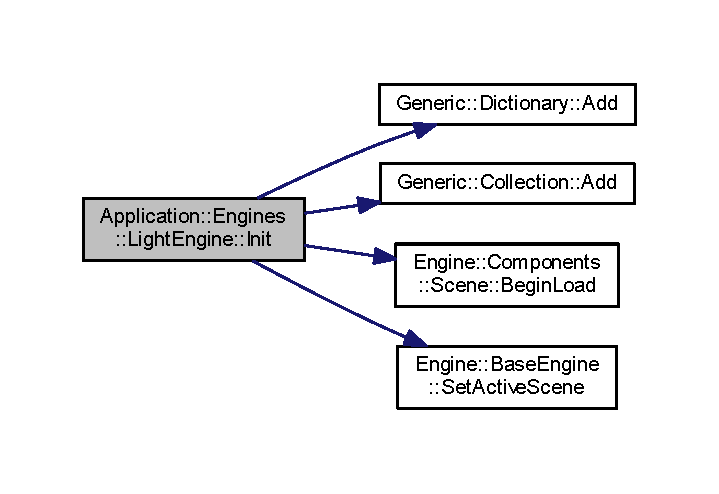
\includegraphics[width=345pt]{classApplication_1_1Engines_1_1LightEngine_ad992d8a300f099c247d7ba8dc38883ea_cgraph}
\end{center}
\end{figure}
\mbox{\Hypertarget{classEngine_1_1BaseEngine_a7a1c9b833049b3eb61194cab113dfe89}\label{classEngine_1_1BaseEngine_a7a1c9b833049b3eb61194cab113dfe89}} 
\index{Application\+::\+Engines\+::\+Light\+Engine@{Application\+::\+Engines\+::\+Light\+Engine}!Init\+Success@{Init\+Success}}
\index{Init\+Success@{Init\+Success}!Application\+::\+Engines\+::\+Light\+Engine@{Application\+::\+Engines\+::\+Light\+Engine}}
\subsubsection{\texorpdfstring{Init\+Success()}{InitSuccess()}}
{\footnotesize\ttfamily bool Engine\+::\+Base\+Engine\+::\+Init\+Success (\begin{DoxyParamCaption}{ }\end{DoxyParamCaption})\hspace{0.3cm}{\ttfamily [inherited]}}



Definition at line 46 of file Base\+Engine.\+cpp.


\begin{DoxyCode}
47 \{
48     \textcolor{keywordflow}{return} \mbox{\hyperlink{classEngine_1_1BaseEngine_a79e265845b321c0e9822fb170c564e55}{\_init}};
49 \}
\end{DoxyCode}
\mbox{\Hypertarget{classEngine_1_1BaseEngine_afc82c6a00d5a9d4714740fc5eab5db86}\label{classEngine_1_1BaseEngine_afc82c6a00d5a9d4714740fc5eab5db86}} 
\index{Application\+::\+Engines\+::\+Light\+Engine@{Application\+::\+Engines\+::\+Light\+Engine}!Set\+Active\+Scene@{Set\+Active\+Scene}}
\index{Set\+Active\+Scene@{Set\+Active\+Scene}!Application\+::\+Engines\+::\+Light\+Engine@{Application\+::\+Engines\+::\+Light\+Engine}}
\subsubsection{\texorpdfstring{Set\+Active\+Scene()}{SetActiveScene()}}
{\footnotesize\ttfamily void Engine\+::\+Base\+Engine\+::\+Set\+Active\+Scene (\begin{DoxyParamCaption}\item[{\mbox{\hyperlink{classEngine_1_1Components_1_1Scene}{Components\+::\+Scene}} $\ast$}]{scene = {\ttfamily nullptr} }\end{DoxyParamCaption})\hspace{0.3cm}{\ttfamily [virtual]}, {\ttfamily [inherited]}}



Definition at line 132 of file Base\+Engine.\+cpp.



Referenced by Application\+::\+Engines\+::\+Basic\+Engine\+::\+Init(), Application\+::\+Engines\+::\+Z\+P\+G\+Engine\+::\+Init(), Application\+::\+Engines\+::\+Triangle\+Engine\+::\+Init(), Application\+::\+Engines\+::\+Camera\+Engine\+::\+Init(), and Init().


\begin{DoxyCode}
133 \{
134     \textcolor{keywordflow}{if} (scene == \textcolor{keyword}{nullptr} && !\mbox{\hyperlink{classEngine_1_1BaseEngine_afd02af3c2fbe9bb734db014dec06585a}{Scenes}}->empty())
135         \mbox{\hyperlink{classEngine_1_1BaseEngine_adb3dbc839da9d821e08b18d8a221698d}{ActiveScene}} = \mbox{\hyperlink{classEngine_1_1BaseEngine_afd02af3c2fbe9bb734db014dec06585a}{Scenes}}->begin()->second;
136     \textcolor{keywordflow}{else}
137         \mbox{\hyperlink{classEngine_1_1BaseEngine_adb3dbc839da9d821e08b18d8a221698d}{ActiveScene}} = scene;     
138 \}
\end{DoxyCode}
Here is the caller graph for this function\+:
\nopagebreak
\begin{figure}[H]
\begin{center}
\leavevmode
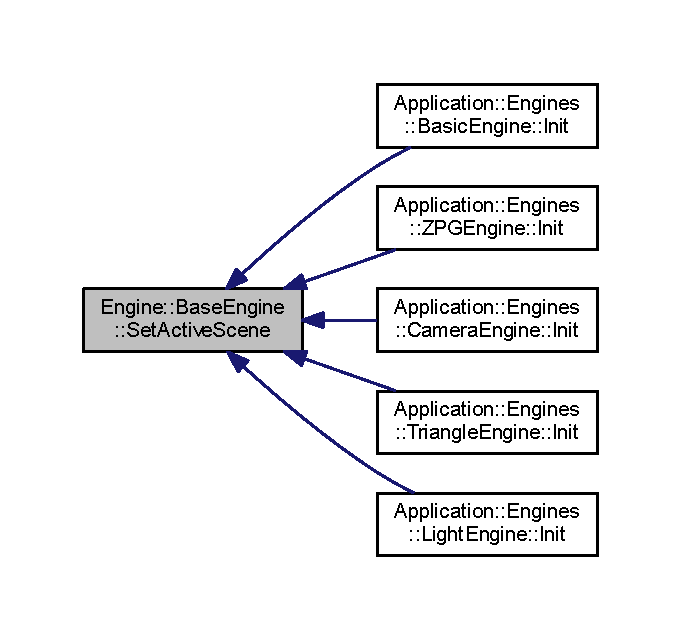
\includegraphics[width=327pt]{classEngine_1_1BaseEngine_afc82c6a00d5a9d4714740fc5eab5db86_icgraph}
\end{center}
\end{figure}
\mbox{\Hypertarget{classEngine_1_1BaseEngine_a525fdc7a1da7eecb514ad5763f06be79}\label{classEngine_1_1BaseEngine_a525fdc7a1da7eecb514ad5763f06be79}} 
\index{Application\+::\+Engines\+::\+Light\+Engine@{Application\+::\+Engines\+::\+Light\+Engine}!Start@{Start}}
\index{Start@{Start}!Application\+::\+Engines\+::\+Light\+Engine@{Application\+::\+Engines\+::\+Light\+Engine}}
\subsubsection{\texorpdfstring{Start()}{Start()}}
{\footnotesize\ttfamily void Engine\+::\+Base\+Engine\+::\+Start (\begin{DoxyParamCaption}{ }\end{DoxyParamCaption})\hspace{0.3cm}{\ttfamily [virtual]}, {\ttfamily [inherited]}}



Definition at line 126 of file Base\+Engine.\+cpp.



Referenced by main().


\begin{DoxyCode}
127 \{
128     system(\textcolor{stringliteral}{"cls"});
129     \mbox{\hyperlink{classEngine_1_1BaseEngine_aad3c237ca657b9f22f76fccf7fc7561f}{UpdateInternal}}();
130 \}
\end{DoxyCode}
Here is the caller graph for this function\+:
\nopagebreak
\begin{figure}[H]
\begin{center}
\leavevmode
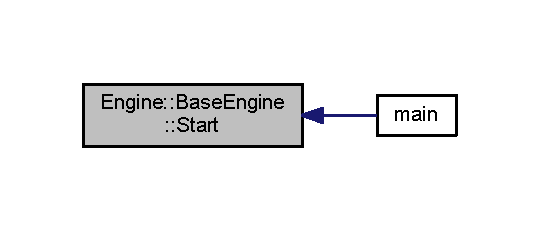
\includegraphics[width=259pt]{classEngine_1_1BaseEngine_a525fdc7a1da7eecb514ad5763f06be79_icgraph}
\end{center}
\end{figure}
\mbox{\Hypertarget{classApplication_1_1Engines_1_1LightEngine_a18575df6f8742099ae543e3b23508ee9}\label{classApplication_1_1Engines_1_1LightEngine_a18575df6f8742099ae543e3b23508ee9}} 
\index{Application\+::\+Engines\+::\+Light\+Engine@{Application\+::\+Engines\+::\+Light\+Engine}!Update@{Update}}
\index{Update@{Update}!Application\+::\+Engines\+::\+Light\+Engine@{Application\+::\+Engines\+::\+Light\+Engine}}
\subsubsection{\texorpdfstring{Update()}{Update()}\hspace{0.1cm}{\footnotesize\ttfamily [1/2]}}
{\footnotesize\ttfamily void Application\+::\+Engines\+::\+Light\+Engine\+::\+Update (\begin{DoxyParamCaption}\item[{\+::\mbox{\hyperlink{classEngine_1_1Components_1_1Window}{Engine\+::\+Components\+::\+Window}} $\ast$}]{window }\end{DoxyParamCaption})\hspace{0.3cm}{\ttfamily [override]}}



Definition at line 213 of file Ligt\+Engine.\+cpp.


\begin{DoxyCode}
214 \{
215     std::cout << \textcolor{stringliteral}{"PS: "} << \mbox{\hyperlink{classApplication_1_1Engines_1_1LightEngine_a5da28beed5c8d278c3615974d464f246}{specularSize}} << \textcolor{stringliteral}{"\(\backslash\)nSS: "} << 
      \mbox{\hyperlink{classApplication_1_1Engines_1_1LightEngine_a97dc7516071da727bcbb137e0cb75301}{specularStrength}} << \textcolor{stringliteral}{"\(\backslash\)nDS: "} << \mbox{\hyperlink{classApplication_1_1Engines_1_1LightEngine_ab2f3fb68d22dd1e6386833f4790a8eb6}{diffuseStrength}} << \textcolor{stringliteral}{"\(\backslash\)nAS: "} << 
      \mbox{\hyperlink{classApplication_1_1Engines_1_1LightEngine_af97d743158c0e55c754b455e7066e6b0}{ambientStrength}} << \textcolor{stringliteral}{"\(\backslash\)nLP: "} << \mbox{\hyperlink{classEngine_1_1BaseEngine_adb3dbc839da9d821e08b18d8a221698d}{ActiveScene}}->\mbox{\hyperlink{classEngine_1_1Components_1_1Scene_a00f60de2f6c72242a7af0076a3b75e5e}{Lights}}->
      \mbox{\hyperlink{classGeneric_1_1Dictionary_ab368d54de28e7a3514e1add4bb5b3a36}{First}}()->\mbox{\hyperlink{classLight_a161f4944da390d9bc388091bafd59fe3}{Power}} << std::endl;
216     
217     \textcolor{keywordflow}{if} (\mbox{\hyperlink{classEngine_1_1BaseEngine_adb3dbc839da9d821e08b18d8a221698d}{ActiveScene}} != \textcolor{keyword}{nullptr} && \mbox{\hyperlink{classEngine_1_1BaseEngine_adb3dbc839da9d821e08b18d8a221698d}{ActiveScene}}->\mbox{\hyperlink{classEngine_1_1Components_1_1Scene_a23481feabaaa56bf5613765db03af4da}{Objects}} != \textcolor{keyword}{nullptr} && !
      \mbox{\hyperlink{classEngine_1_1BaseEngine_adb3dbc839da9d821e08b18d8a221698d}{ActiveScene}}->\mbox{\hyperlink{classEngine_1_1Components_1_1Scene_a23481feabaaa56bf5613765db03af4da}{Objects}}->empty())
218         \textcolor{keywordflow}{for} (\textcolor{keyword}{auto}& it : *\mbox{\hyperlink{classEngine_1_1BaseEngine_adb3dbc839da9d821e08b18d8a221698d}{ActiveScene}}->\mbox{\hyperlink{classEngine_1_1Components_1_1Scene_a23481feabaaa56bf5613765db03af4da}{Objects}})
219         \{
220             \textcolor{comment}{/*auto \_fi = glm::radians(90.f*(MouseX / window->Height));}
221 \textcolor{comment}{            auto \_psi = glm::radians(90.f*(MouseY / window->Width));}
222 \textcolor{comment}{}
223 \textcolor{comment}{            std::cout << "FI:  " << \_fi << "\(\backslash\)nPSI: " << \_psi << "\(\backslash\)nObject: " << it.first << std::endl;}
224 \textcolor{comment}{            */}
225             \textcolor{comment}{//ActiveScene->Cameras->First()->SetDirection(new glm::vec3(cos(\_fi), sin(\_fi), cos(\_psi)));}
226 
227             \textcolor{keyword}{auto} \textcolor{keywordtype}{object} = it.second;
228             \textcolor{keywordtype}{object}->Draw();
229             
230             \mbox{\hyperlink{classApplication_1_1Engines_1_1LightEngine_ad729a37b02875c824d6bd2c8630a4520}{angle}} += 0.1f;
231         \}
232 \}
\end{DoxyCode}
\mbox{\Hypertarget{classEngine_1_1BaseEngine_a01c23c2073f08939a660f3b7a866852c}\label{classEngine_1_1BaseEngine_a01c23c2073f08939a660f3b7a866852c}} 
\index{Application\+::\+Engines\+::\+Light\+Engine@{Application\+::\+Engines\+::\+Light\+Engine}!Update@{Update}}
\index{Update@{Update}!Application\+::\+Engines\+::\+Light\+Engine@{Application\+::\+Engines\+::\+Light\+Engine}}
\subsubsection{\texorpdfstring{Update()}{Update()}\hspace{0.1cm}{\footnotesize\ttfamily [2/2]}}
{\footnotesize\ttfamily void Engine\+::\+Base\+Engine\+::\+Update (\begin{DoxyParamCaption}\item[{\mbox{\hyperlink{classEngine_1_1Components_1_1Window}{Components\+::\+Window}} $\ast$}]{window }\end{DoxyParamCaption})\hspace{0.3cm}{\ttfamily [virtual]}, {\ttfamily [inherited]}}



Definition at line 112 of file Base\+Engine.\+cpp.


\begin{DoxyCode}
113 \{
114 \}
\end{DoxyCode}
\mbox{\Hypertarget{classEngine_1_1BaseEngine_aace6be2a42d12b64fbd35f1acdb08408}\label{classEngine_1_1BaseEngine_aace6be2a42d12b64fbd35f1acdb08408}} 
\index{Application\+::\+Engines\+::\+Light\+Engine@{Application\+::\+Engines\+::\+Light\+Engine}!Update\+Begin@{Update\+Begin}}
\index{Update\+Begin@{Update\+Begin}!Application\+::\+Engines\+::\+Light\+Engine@{Application\+::\+Engines\+::\+Light\+Engine}}
\subsubsection{\texorpdfstring{Update\+Begin()}{UpdateBegin()}}
{\footnotesize\ttfamily void Engine\+::\+Base\+Engine\+::\+Update\+Begin (\begin{DoxyParamCaption}\item[{\mbox{\hyperlink{classEngine_1_1Components_1_1Window}{Components\+::\+Window}} $\ast$}]{window }\end{DoxyParamCaption})\hspace{0.3cm}{\ttfamily [virtual]}, {\ttfamily [inherited]}}



Definition at line 57 of file Base\+Engine.\+cpp.



References Engine\+::\+Components\+::\+Window\+::\+Get().


\begin{DoxyCode}
58 \{
59     \textcolor{comment}{// Scene}
60     \mbox{\hyperlink{classEngine_1_1BaseEngine_adb3dbc839da9d821e08b18d8a221698d}{ActiveScene}}->\mbox{\hyperlink{classEngine_1_1Components_1_1Scene_af18bd334fe66952b8d79b8e9e99ab2d8}{BeginLoad}}(\textcolor{keyword}{this});
61 
62     \textcolor{comment}{// Buffers}
63     glEnable(GL\_DEPTH\_TEST);
64     glDepthFunc(GL\_LESS);
65     glClear(GL\_COLOR\_BUFFER\_BIT | GL\_DEPTH\_BUFFER\_BIT);
66 
67     \textcolor{comment}{// Input}
68     \textcolor{keywordtype}{short} mouseKeysActive = 0;
69     glfwGetCursorPos(window->Get(), &\mbox{\hyperlink{classEngine_1_1BaseEngine_a5fe085152ebe93346900407f6b41a034}{MouseX}}, &\mbox{\hyperlink{classEngine_1_1BaseEngine_a143c9c32dbbdc70bf1546ffe275bf384}{MouseY}});
70     \textcolor{keywordflow}{for}(\textcolor{keywordtype}{short} i = 0; i < 8; i++)
71     \{
72         \textcolor{keyword}{const} \textcolor{keywordtype}{int} state = glfwGetMouseButton(window->Get(), i);
73         \textcolor{keyword}{auto} value = \mbox{\hyperlink{classEngine_1_1BaseEngine_a3ee2bdddb66d45b8c808ffd937ba9c50}{MouseKeys}}[i];
74         \textcolor{comment}{// flip state}
75         \textcolor{keywordflow}{if} (state == GLFW\_PRESS && !value)
76             \mbox{\hyperlink{classEngine_1_1BaseEngine_a3ee2bdddb66d45b8c808ffd937ba9c50}{MouseKeys}}.\mbox{\hyperlink{classGeneric_1_1Dictionary_ae7cb006f801b21c172e8fbac8794fa99}{Add}}(i, \textcolor{keyword}{true});
77         \textcolor{keywordflow}{else} \textcolor{keywordflow}{if} (state == GLFW\_RELEASE && value)
78             \mbox{\hyperlink{classEngine_1_1BaseEngine_a3ee2bdddb66d45b8c808ffd937ba9c50}{MouseKeys}}.\mbox{\hyperlink{classGeneric_1_1Dictionary_ae7cb006f801b21c172e8fbac8794fa99}{Add}}(i, \textcolor{keyword}{false});
79         \textcolor{keywordflow}{if} (\mbox{\hyperlink{classEngine_1_1BaseEngine_a3ee2bdddb66d45b8c808ffd937ba9c50}{MouseKeys}}[i])
80             mouseKeysActive++;
81     \}
82     \textcolor{keywordtype}{short} keysActive = 0;
83     SetConsoleCursorPosition(GetStdHandle(STD\_OUTPUT\_HANDLE), \{ 40, keysActive \});
84     fprintf(\mbox{\hyperlink{classEngine_1_1BaseEngine_a26fd54a1ee2733f9c654af5afcfa96cf}{\_errorStream}}, \textcolor{stringliteral}{"                           "});
85     \textcolor{keywordflow}{for} (\textcolor{keywordtype}{short} i = 1; i < 512; i++)
86     \{
87         \textcolor{keyword}{const} \textcolor{keywordtype}{int} state = glfwGetKey(window->Get(), i);
88         \textcolor{keyword}{auto} value = \mbox{\hyperlink{classEngine_1_1BaseEngine_a65321a97e83f0a6ee90df3efac2d3307}{Keys}}[i];
89         \textcolor{comment}{// flip state}
90         \textcolor{keywordflow}{if} (state == GLFW\_PRESS && !value)
91             \mbox{\hyperlink{classEngine_1_1BaseEngine_a65321a97e83f0a6ee90df3efac2d3307}{Keys}}.\mbox{\hyperlink{classGeneric_1_1Dictionary_ae7cb006f801b21c172e8fbac8794fa99}{Add}}(i, \textcolor{keyword}{true});
92         \textcolor{keywordflow}{else} \textcolor{keywordflow}{if} (state == GLFW\_RELEASE && value)
93             \mbox{\hyperlink{classEngine_1_1BaseEngine_a65321a97e83f0a6ee90df3efac2d3307}{Keys}}.\mbox{\hyperlink{classGeneric_1_1Dictionary_ae7cb006f801b21c172e8fbac8794fa99}{Add}}(i, \textcolor{keyword}{false});
94         \textcolor{keywordflow}{if} (\mbox{\hyperlink{classEngine_1_1BaseEngine_a65321a97e83f0a6ee90df3efac2d3307}{Keys}}[i])
95             keysActive++;
96     \}
97     \textcolor{keywordtype}{bool} handleKeys = \textcolor{keyword}{true},
98          handleMouse = \textcolor{keyword}{true};
99     \textcolor{keywordflow}{for} (\textcolor{keyword}{auto} handler : *\mbox{\hyperlink{classEngine_1_1BaseEngine_a134fa082c5a64d62b76ddf926647e7cc}{InputHandlers}})
100     \{
101         \textcolor{keywordflow}{if}(handleKeys)
102             handleKeys = handler->HandleKeys(\textcolor{keyword}{this}, window, \mbox{\hyperlink{classEngine_1_1BaseEngine_adb3dbc839da9d821e08b18d8a221698d}{ActiveScene}}, 
      \mbox{\hyperlink{classEngine_1_1BaseEngine_a65321a97e83f0a6ee90df3efac2d3307}{Keys}}, keysActive);
103         \textcolor{keywordflow}{if}(handleMouse)
104             handleMouse = handler->HandleMouse(\textcolor{keyword}{this}, window, \mbox{\hyperlink{classEngine_1_1BaseEngine_adb3dbc839da9d821e08b18d8a221698d}{ActiveScene}}, 
      \mbox{\hyperlink{classEngine_1_1BaseEngine_a5fe085152ebe93346900407f6b41a034}{MouseX}}, \mbox{\hyperlink{classEngine_1_1BaseEngine_a143c9c32dbbdc70bf1546ffe275bf384}{MouseY}}, \mbox{\hyperlink{classEngine_1_1BaseEngine_a3ee2bdddb66d45b8c808ffd937ba9c50}{MouseKeys}}, mouseKeysActive);
105         \textcolor{keywordflow}{if}(!handleKeys && !handleMouse)
106             \textcolor{keywordflow}{break};
107     \}
108 
109     SetConsoleCursorPosition(GetStdHandle(STD\_OUTPUT\_HANDLE), \{ 0,0 \});
110 \}
\end{DoxyCode}
Here is the call graph for this function\+:
\nopagebreak
\begin{figure}[H]
\begin{center}
\leavevmode
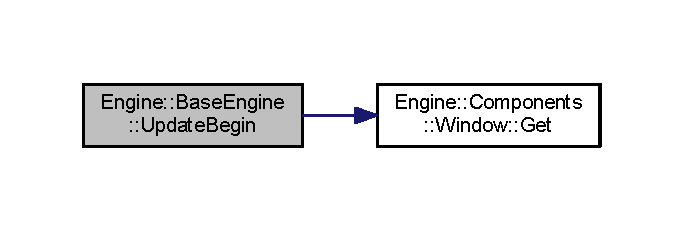
\includegraphics[width=328pt]{classEngine_1_1BaseEngine_aace6be2a42d12b64fbd35f1acdb08408_cgraph}
\end{center}
\end{figure}
\mbox{\Hypertarget{classEngine_1_1BaseEngine_a7c07c98e583df042a0eb01e0ddec85a1}\label{classEngine_1_1BaseEngine_a7c07c98e583df042a0eb01e0ddec85a1}} 
\index{Application\+::\+Engines\+::\+Light\+Engine@{Application\+::\+Engines\+::\+Light\+Engine}!Update\+End@{Update\+End}}
\index{Update\+End@{Update\+End}!Application\+::\+Engines\+::\+Light\+Engine@{Application\+::\+Engines\+::\+Light\+Engine}}
\subsubsection{\texorpdfstring{Update\+End()}{UpdateEnd()}}
{\footnotesize\ttfamily void Engine\+::\+Base\+Engine\+::\+Update\+End (\begin{DoxyParamCaption}\item[{\mbox{\hyperlink{classEngine_1_1Components_1_1Window}{Components\+::\+Window}} $\ast$}]{window }\end{DoxyParamCaption})\hspace{0.3cm}{\ttfamily [virtual]}, {\ttfamily [inherited]}}



Definition at line 116 of file Base\+Engine.\+cpp.



References Engine\+::\+Components\+::\+Window\+::\+Get().


\begin{DoxyCode}
117 \{
118     \textcolor{comment}{// update other events like input handling}
119     glfwPollEvents();
120     \textcolor{comment}{// put the stuff we’ve been drawing onto the display}
121     glfwSwapBuffers(window->Get());
122 
123     \mbox{\hyperlink{classEngine_1_1BaseEngine_adb3dbc839da9d821e08b18d8a221698d}{ActiveScene}}->\mbox{\hyperlink{classEngine_1_1Components_1_1Scene_abd8fcdcac52dbce6a0a18de3860ab087}{FrameUpdate}}(\textcolor{keyword}{this});
124 \}
\end{DoxyCode}
Here is the call graph for this function\+:
\nopagebreak
\begin{figure}[H]
\begin{center}
\leavevmode
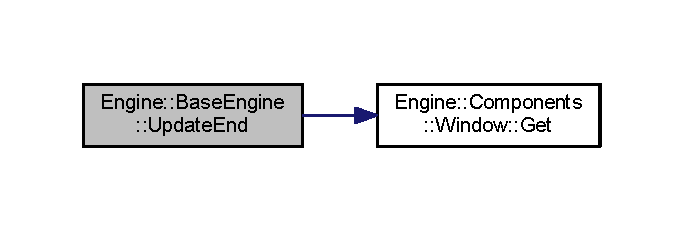
\includegraphics[width=328pt]{classEngine_1_1BaseEngine_a7c07c98e583df042a0eb01e0ddec85a1_cgraph}
\end{center}
\end{figure}


\subsection{Member Data Documentation}
\mbox{\Hypertarget{classEngine_1_1BaseEngine_adb3dbc839da9d821e08b18d8a221698d}\label{classEngine_1_1BaseEngine_adb3dbc839da9d821e08b18d8a221698d}} 
\index{Application\+::\+Engines\+::\+Light\+Engine@{Application\+::\+Engines\+::\+Light\+Engine}!Active\+Scene@{Active\+Scene}}
\index{Active\+Scene@{Active\+Scene}!Application\+::\+Engines\+::\+Light\+Engine@{Application\+::\+Engines\+::\+Light\+Engine}}
\subsubsection{\texorpdfstring{Active\+Scene}{ActiveScene}}
{\footnotesize\ttfamily Components\+::\+Scene$\ast$ Engine\+::\+Base\+Engine\+::\+Active\+Scene\hspace{0.3cm}{\ttfamily [inherited]}}



Definition at line 34 of file Base\+Engine.\+h.



Referenced by Engine\+::\+Base\+Engine\+::\+Base\+Engine(), Application\+::\+Engines\+::\+Camera\+Engine\+::\+Init(), and Init().

\mbox{\Hypertarget{classApplication_1_1Engines_1_1LightEngine_ab22b7d03d1c3cd19214474fb56bdd2ee}\label{classApplication_1_1Engines_1_1LightEngine_ab22b7d03d1c3cd19214474fb56bdd2ee}} 
\index{Application\+::\+Engines\+::\+Light\+Engine@{Application\+::\+Engines\+::\+Light\+Engine}!ambient\+Color@{ambient\+Color}}
\index{ambient\+Color@{ambient\+Color}!Application\+::\+Engines\+::\+Light\+Engine@{Application\+::\+Engines\+::\+Light\+Engine}}
\subsubsection{\texorpdfstring{ambient\+Color}{ambientColor}}
{\footnotesize\ttfamily glm\+::vec3 Application\+::\+Engines\+::\+Light\+Engine\+::ambient\+Color}



Definition at line 17 of file Ligt\+Engine.\+h.



Referenced by Init().

\mbox{\Hypertarget{classApplication_1_1Engines_1_1LightEngine_af97d743158c0e55c754b455e7066e6b0}\label{classApplication_1_1Engines_1_1LightEngine_af97d743158c0e55c754b455e7066e6b0}} 
\index{Application\+::\+Engines\+::\+Light\+Engine@{Application\+::\+Engines\+::\+Light\+Engine}!ambient\+Strength@{ambient\+Strength}}
\index{ambient\+Strength@{ambient\+Strength}!Application\+::\+Engines\+::\+Light\+Engine@{Application\+::\+Engines\+::\+Light\+Engine}}
\subsubsection{\texorpdfstring{ambient\+Strength}{ambientStrength}}
{\footnotesize\ttfamily float Application\+::\+Engines\+::\+Light\+Engine\+::ambient\+Strength}



Definition at line 14 of file Ligt\+Engine.\+h.



Referenced by Init().

\mbox{\Hypertarget{classApplication_1_1Engines_1_1LightEngine_ad729a37b02875c824d6bd2c8630a4520}\label{classApplication_1_1Engines_1_1LightEngine_ad729a37b02875c824d6bd2c8630a4520}} 
\index{Application\+::\+Engines\+::\+Light\+Engine@{Application\+::\+Engines\+::\+Light\+Engine}!angle@{angle}}
\index{angle@{angle}!Application\+::\+Engines\+::\+Light\+Engine@{Application\+::\+Engines\+::\+Light\+Engine}}
\subsubsection{\texorpdfstring{angle}{angle}}
{\footnotesize\ttfamily float Application\+::\+Engines\+::\+Light\+Engine\+::angle\hspace{0.3cm}{\ttfamily [private]}}



Definition at line 23 of file Ligt\+Engine.\+h.



Referenced by Init().

\mbox{\Hypertarget{classApplication_1_1Engines_1_1LightEngine_a2247de4ba43b8d0e159ab90edd581363}\label{classApplication_1_1Engines_1_1LightEngine_a2247de4ba43b8d0e159ab90edd581363}} 
\index{Application\+::\+Engines\+::\+Light\+Engine@{Application\+::\+Engines\+::\+Light\+Engine}!diffuse\+Color@{diffuse\+Color}}
\index{diffuse\+Color@{diffuse\+Color}!Application\+::\+Engines\+::\+Light\+Engine@{Application\+::\+Engines\+::\+Light\+Engine}}
\subsubsection{\texorpdfstring{diffuse\+Color}{diffuseColor}}
{\footnotesize\ttfamily glm\+::vec3 Application\+::\+Engines\+::\+Light\+Engine\+::diffuse\+Color}



Definition at line 18 of file Ligt\+Engine.\+h.



Referenced by Init().

\mbox{\Hypertarget{classApplication_1_1Engines_1_1LightEngine_ab2f3fb68d22dd1e6386833f4790a8eb6}\label{classApplication_1_1Engines_1_1LightEngine_ab2f3fb68d22dd1e6386833f4790a8eb6}} 
\index{Application\+::\+Engines\+::\+Light\+Engine@{Application\+::\+Engines\+::\+Light\+Engine}!diffuse\+Strength@{diffuse\+Strength}}
\index{diffuse\+Strength@{diffuse\+Strength}!Application\+::\+Engines\+::\+Light\+Engine@{Application\+::\+Engines\+::\+Light\+Engine}}
\subsubsection{\texorpdfstring{diffuse\+Strength}{diffuseStrength}}
{\footnotesize\ttfamily float Application\+::\+Engines\+::\+Light\+Engine\+::diffuse\+Strength}



Definition at line 15 of file Ligt\+Engine.\+h.



Referenced by Init().

\mbox{\Hypertarget{classEngine_1_1BaseEngine_a134fa082c5a64d62b76ddf926647e7cc}\label{classEngine_1_1BaseEngine_a134fa082c5a64d62b76ddf926647e7cc}} 
\index{Application\+::\+Engines\+::\+Light\+Engine@{Application\+::\+Engines\+::\+Light\+Engine}!Input\+Handlers@{Input\+Handlers}}
\index{Input\+Handlers@{Input\+Handlers}!Application\+::\+Engines\+::\+Light\+Engine@{Application\+::\+Engines\+::\+Light\+Engine}}
\subsubsection{\texorpdfstring{Input\+Handlers}{InputHandlers}}
{\footnotesize\ttfamily \mbox{\hyperlink{classGeneric_1_1Collection}{Generic\+::\+Collection}}$<$Components\+::\+I\+Input\+Handler$\ast$$>$$\ast$ Engine\+::\+Base\+Engine\+::\+Input\+Handlers\hspace{0.3cm}{\ttfamily [inherited]}}



Definition at line 31 of file Base\+Engine.\+h.



Referenced by Engine\+::\+Base\+Engine\+::\+Base\+Engine(), and Init().

\mbox{\Hypertarget{classEngine_1_1BaseEngine_a65321a97e83f0a6ee90df3efac2d3307}\label{classEngine_1_1BaseEngine_a65321a97e83f0a6ee90df3efac2d3307}} 
\index{Application\+::\+Engines\+::\+Light\+Engine@{Application\+::\+Engines\+::\+Light\+Engine}!Keys@{Keys}}
\index{Keys@{Keys}!Application\+::\+Engines\+::\+Light\+Engine@{Application\+::\+Engines\+::\+Light\+Engine}}
\subsubsection{\texorpdfstring{Keys}{Keys}}
{\footnotesize\ttfamily \mbox{\hyperlink{classGeneric_1_1Dictionary}{Generic\+::\+Dictionary}}$<$short, bool$>$ Engine\+::\+Base\+Engine\+::\+Keys\hspace{0.3cm}{\ttfamily [inherited]}}



Definition at line 32 of file Base\+Engine.\+h.



Referenced by Engine\+::\+Base\+Engine\+::\+Base\+Engine().

\mbox{\Hypertarget{classApplication_1_1Engines_1_1LightEngine_ae9cca787b2b0d5d4dbcc3c63afa196e1}\label{classApplication_1_1Engines_1_1LightEngine_ae9cca787b2b0d5d4dbcc3c63afa196e1}} 
\index{Application\+::\+Engines\+::\+Light\+Engine@{Application\+::\+Engines\+::\+Light\+Engine}!M@{M}}
\index{M@{M}!Application\+::\+Engines\+::\+Light\+Engine@{Application\+::\+Engines\+::\+Light\+Engine}}
\subsubsection{\texorpdfstring{M}{M}}
{\footnotesize\ttfamily glm\+::mat4 Application\+::\+Engines\+::\+Light\+Engine\+::M\hspace{0.3cm}{\ttfamily [private]}}



Definition at line 22 of file Ligt\+Engine.\+h.



Referenced by Init().

\mbox{\Hypertarget{classEngine_1_1BaseEngine_a3ee2bdddb66d45b8c808ffd937ba9c50}\label{classEngine_1_1BaseEngine_a3ee2bdddb66d45b8c808ffd937ba9c50}} 
\index{Application\+::\+Engines\+::\+Light\+Engine@{Application\+::\+Engines\+::\+Light\+Engine}!Mouse\+Keys@{Mouse\+Keys}}
\index{Mouse\+Keys@{Mouse\+Keys}!Application\+::\+Engines\+::\+Light\+Engine@{Application\+::\+Engines\+::\+Light\+Engine}}
\subsubsection{\texorpdfstring{Mouse\+Keys}{MouseKeys}}
{\footnotesize\ttfamily \mbox{\hyperlink{classGeneric_1_1Dictionary}{Generic\+::\+Dictionary}}$<$short, bool$>$ Engine\+::\+Base\+Engine\+::\+Mouse\+Keys\hspace{0.3cm}{\ttfamily [inherited]}}



Definition at line 33 of file Base\+Engine.\+h.



Referenced by Engine\+::\+Base\+Engine\+::\+Base\+Engine().

\mbox{\Hypertarget{classEngine_1_1BaseEngine_a5fe085152ebe93346900407f6b41a034}\label{classEngine_1_1BaseEngine_a5fe085152ebe93346900407f6b41a034}} 
\index{Application\+::\+Engines\+::\+Light\+Engine@{Application\+::\+Engines\+::\+Light\+Engine}!MouseX@{MouseX}}
\index{MouseX@{MouseX}!Application\+::\+Engines\+::\+Light\+Engine@{Application\+::\+Engines\+::\+Light\+Engine}}
\subsubsection{\texorpdfstring{MouseX}{MouseX}}
{\footnotesize\ttfamily double Engine\+::\+Base\+Engine\+::\+MouseX\hspace{0.3cm}{\ttfamily [inherited]}}



Definition at line 35 of file Base\+Engine.\+h.

\mbox{\Hypertarget{classEngine_1_1BaseEngine_a143c9c32dbbdc70bf1546ffe275bf384}\label{classEngine_1_1BaseEngine_a143c9c32dbbdc70bf1546ffe275bf384}} 
\index{Application\+::\+Engines\+::\+Light\+Engine@{Application\+::\+Engines\+::\+Light\+Engine}!MouseY@{MouseY}}
\index{MouseY@{MouseY}!Application\+::\+Engines\+::\+Light\+Engine@{Application\+::\+Engines\+::\+Light\+Engine}}
\subsubsection{\texorpdfstring{MouseY}{MouseY}}
{\footnotesize\ttfamily double Engine\+::\+Base\+Engine\+::\+MouseY\hspace{0.3cm}{\ttfamily [inherited]}}



Definition at line 36 of file Base\+Engine.\+h.

\mbox{\Hypertarget{classEngine_1_1BaseEngine_ae0f86360ea3a384caefe443dd8f88601}\label{classEngine_1_1BaseEngine_ae0f86360ea3a384caefe443dd8f88601}} 
\index{Application\+::\+Engines\+::\+Light\+Engine@{Application\+::\+Engines\+::\+Light\+Engine}!Programs@{Programs}}
\index{Programs@{Programs}!Application\+::\+Engines\+::\+Light\+Engine@{Application\+::\+Engines\+::\+Light\+Engine}}
\subsubsection{\texorpdfstring{Programs}{Programs}}
{\footnotesize\ttfamily \mbox{\hyperlink{classGeneric_1_1Dictionary}{Generic\+::\+Dictionary}}$<$std\+::string, Components\+::\+Graphics\+::\+Program$\ast$$>$$\ast$ Engine\+::\+Base\+Engine\+::\+Programs\hspace{0.3cm}{\ttfamily [inherited]}}



Definition at line 28 of file Base\+Engine.\+h.



Referenced by Engine\+::\+Base\+Engine\+::\+Base\+Engine(), Application\+::\+Input\+::\+Handlers\+::\+Camera\+Input\+Handler\+::\+Handle\+Mouse(), Application\+::\+Engines\+::\+Basic\+Engine\+::\+Init(), Application\+::\+Engines\+::\+Camera\+Engine\+::\+Init(), Application\+::\+Engines\+::\+Z\+P\+G\+Engine\+::\+Init(), Application\+::\+Engines\+::\+Triangle\+Engine\+::\+Init(), Init(), Application\+::\+Scenes\+::\+Triangle\+Scene\+::\+Load(), and Application\+::\+Scenes\+::\+Sphere\+Scene\+::\+Load().

\mbox{\Hypertarget{classEngine_1_1BaseEngine_afd02af3c2fbe9bb734db014dec06585a}\label{classEngine_1_1BaseEngine_afd02af3c2fbe9bb734db014dec06585a}} 
\index{Application\+::\+Engines\+::\+Light\+Engine@{Application\+::\+Engines\+::\+Light\+Engine}!Scenes@{Scenes}}
\index{Scenes@{Scenes}!Application\+::\+Engines\+::\+Light\+Engine@{Application\+::\+Engines\+::\+Light\+Engine}}
\subsubsection{\texorpdfstring{Scenes}{Scenes}}
{\footnotesize\ttfamily \mbox{\hyperlink{classGeneric_1_1Dictionary}{Generic\+::\+Dictionary}}$<$std\+::string, Components\+::\+Scene$\ast$$>$$\ast$ Engine\+::\+Base\+Engine\+::\+Scenes\hspace{0.3cm}{\ttfamily [inherited]}}



Definition at line 30 of file Base\+Engine.\+h.



Referenced by Engine\+::\+Base\+Engine\+::\+Base\+Engine(), Application\+::\+Engines\+::\+Z\+P\+G\+Engine\+::\+Init(), Application\+::\+Engines\+::\+Triangle\+Engine\+::\+Init(), Application\+::\+Engines\+::\+Basic\+Engine\+::\+Init(), Application\+::\+Engines\+::\+Camera\+Engine\+::\+Init(), and Init().

\mbox{\Hypertarget{classEngine_1_1BaseEngine_a2582dee3f73da82bb422b43317b85e3b}\label{classEngine_1_1BaseEngine_a2582dee3f73da82bb422b43317b85e3b}} 
\index{Application\+::\+Engines\+::\+Light\+Engine@{Application\+::\+Engines\+::\+Light\+Engine}!Shaders@{Shaders}}
\index{Shaders@{Shaders}!Application\+::\+Engines\+::\+Light\+Engine@{Application\+::\+Engines\+::\+Light\+Engine}}
\subsubsection{\texorpdfstring{Shaders}{Shaders}}
{\footnotesize\ttfamily \mbox{\hyperlink{classGeneric_1_1Dictionary}{Generic\+::\+Dictionary}}$<$std\+::string, Components\+::\+Graphics\+::\+Shader$\ast$$>$$\ast$ Engine\+::\+Base\+Engine\+::\+Shaders\hspace{0.3cm}{\ttfamily [inherited]}}



Definition at line 29 of file Base\+Engine.\+h.



Referenced by Engine\+::\+Base\+Engine\+::\+Base\+Engine(), Application\+::\+Input\+::\+Handlers\+::\+Camera\+Input\+Handler\+::\+Handle\+Mouse(), Application\+::\+Engines\+::\+Triangle\+Engine\+::\+Init(), Application\+::\+Engines\+::\+Z\+P\+G\+Engine\+::\+Init(), Application\+::\+Engines\+::\+Basic\+Engine\+::\+Init(), Application\+::\+Engines\+::\+Camera\+Engine\+::\+Init(), and Init().

\mbox{\Hypertarget{classApplication_1_1Engines_1_1LightEngine_ae03347f7ed935e951726dffba52d0fef}\label{classApplication_1_1Engines_1_1LightEngine_ae03347f7ed935e951726dffba52d0fef}} 
\index{Application\+::\+Engines\+::\+Light\+Engine@{Application\+::\+Engines\+::\+Light\+Engine}!specular\+Color@{specular\+Color}}
\index{specular\+Color@{specular\+Color}!Application\+::\+Engines\+::\+Light\+Engine@{Application\+::\+Engines\+::\+Light\+Engine}}
\subsubsection{\texorpdfstring{specular\+Color}{specularColor}}
{\footnotesize\ttfamily glm\+::vec3 Application\+::\+Engines\+::\+Light\+Engine\+::specular\+Color}



Definition at line 19 of file Ligt\+Engine.\+h.



Referenced by Init().

\mbox{\Hypertarget{classApplication_1_1Engines_1_1LightEngine_a5da28beed5c8d278c3615974d464f246}\label{classApplication_1_1Engines_1_1LightEngine_a5da28beed5c8d278c3615974d464f246}} 
\index{Application\+::\+Engines\+::\+Light\+Engine@{Application\+::\+Engines\+::\+Light\+Engine}!specular\+Size@{specular\+Size}}
\index{specular\+Size@{specular\+Size}!Application\+::\+Engines\+::\+Light\+Engine@{Application\+::\+Engines\+::\+Light\+Engine}}
\subsubsection{\texorpdfstring{specular\+Size}{specularSize}}
{\footnotesize\ttfamily int Application\+::\+Engines\+::\+Light\+Engine\+::specular\+Size}



Definition at line 20 of file Ligt\+Engine.\+h.



Referenced by Application\+::\+Input\+::\+Handlers\+::\+Lighting\+Change\+Input\+Handler\+::\+Handle\+Keys(), and Init().

\mbox{\Hypertarget{classApplication_1_1Engines_1_1LightEngine_a97dc7516071da727bcbb137e0cb75301}\label{classApplication_1_1Engines_1_1LightEngine_a97dc7516071da727bcbb137e0cb75301}} 
\index{Application\+::\+Engines\+::\+Light\+Engine@{Application\+::\+Engines\+::\+Light\+Engine}!specular\+Strength@{specular\+Strength}}
\index{specular\+Strength@{specular\+Strength}!Application\+::\+Engines\+::\+Light\+Engine@{Application\+::\+Engines\+::\+Light\+Engine}}
\subsubsection{\texorpdfstring{specular\+Strength}{specularStrength}}
{\footnotesize\ttfamily float Application\+::\+Engines\+::\+Light\+Engine\+::specular\+Strength}



Definition at line 16 of file Ligt\+Engine.\+h.



Referenced by Init().

\mbox{\Hypertarget{classEngine_1_1BaseEngine_a4a1a4c4dae052e66ecc4f326eeed4d33}\label{classEngine_1_1BaseEngine_a4a1a4c4dae052e66ecc4f326eeed4d33}} 
\index{Application\+::\+Engines\+::\+Light\+Engine@{Application\+::\+Engines\+::\+Light\+Engine}!Windows@{Windows}}
\index{Windows@{Windows}!Application\+::\+Engines\+::\+Light\+Engine@{Application\+::\+Engines\+::\+Light\+Engine}}
\subsubsection{\texorpdfstring{Windows}{Windows}}
{\footnotesize\ttfamily \mbox{\hyperlink{classGeneric_1_1Dictionary}{Generic\+::\+Dictionary}}$<$std\+::string, Components\+::\+Window$\ast$$>$$\ast$ Engine\+::\+Base\+Engine\+::\+Windows\hspace{0.3cm}{\ttfamily [inherited]}}



Definition at line 27 of file Base\+Engine.\+h.



Referenced by Engine\+::\+Base\+Engine\+::\+Base\+Engine(), Application\+::\+Engines\+::\+Z\+P\+G\+Engine\+::\+Init(), Application\+::\+Engines\+::\+Triangle\+Engine\+::\+Init(), Application\+::\+Engines\+::\+Basic\+Engine\+::\+Init(), Application\+::\+Engines\+::\+Camera\+Engine\+::\+Init(), and Init().



The documentation for this class was generated from the following files\+:\begin{DoxyCompactItemize}
\item 
Z\+P\+G/\mbox{\hyperlink{LigtEngine_8h}{Ligt\+Engine.\+h}}\item 
Z\+P\+G/\mbox{\hyperlink{LigtEngine_8cpp}{Ligt\+Engine.\+cpp}}\end{DoxyCompactItemize}

\hypertarget{classApplication_1_1Engines_1_1TriangleEngine}{}\section{Application\+:\+:Engines\+:\+:Triangle\+Engine Class Reference}
\label{classApplication_1_1Engines_1_1TriangleEngine}\index{Application\+::\+Engines\+::\+Triangle\+Engine@{Application\+::\+Engines\+::\+Triangle\+Engine}}


{\ttfamily \#include $<$Triangle\+Engine.\+h$>$}



Inheritance diagram for Application\+:\+:Engines\+:\+:Triangle\+Engine\+:
\nopagebreak
\begin{figure}[H]
\begin{center}
\leavevmode
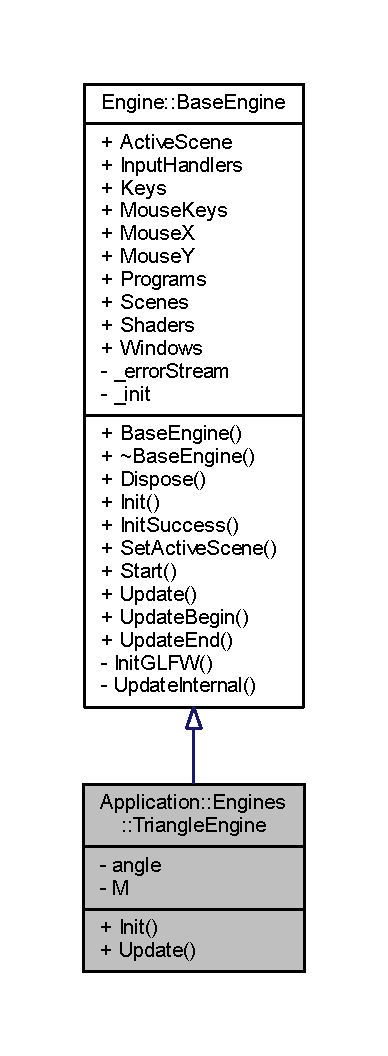
\includegraphics[width=186pt]{classApplication_1_1Engines_1_1TriangleEngine__inherit__graph}
\end{center}
\end{figure}


Collaboration diagram for Application\+:\+:Engines\+:\+:Triangle\+Engine\+:
\nopagebreak
\begin{figure}[H]
\begin{center}
\leavevmode
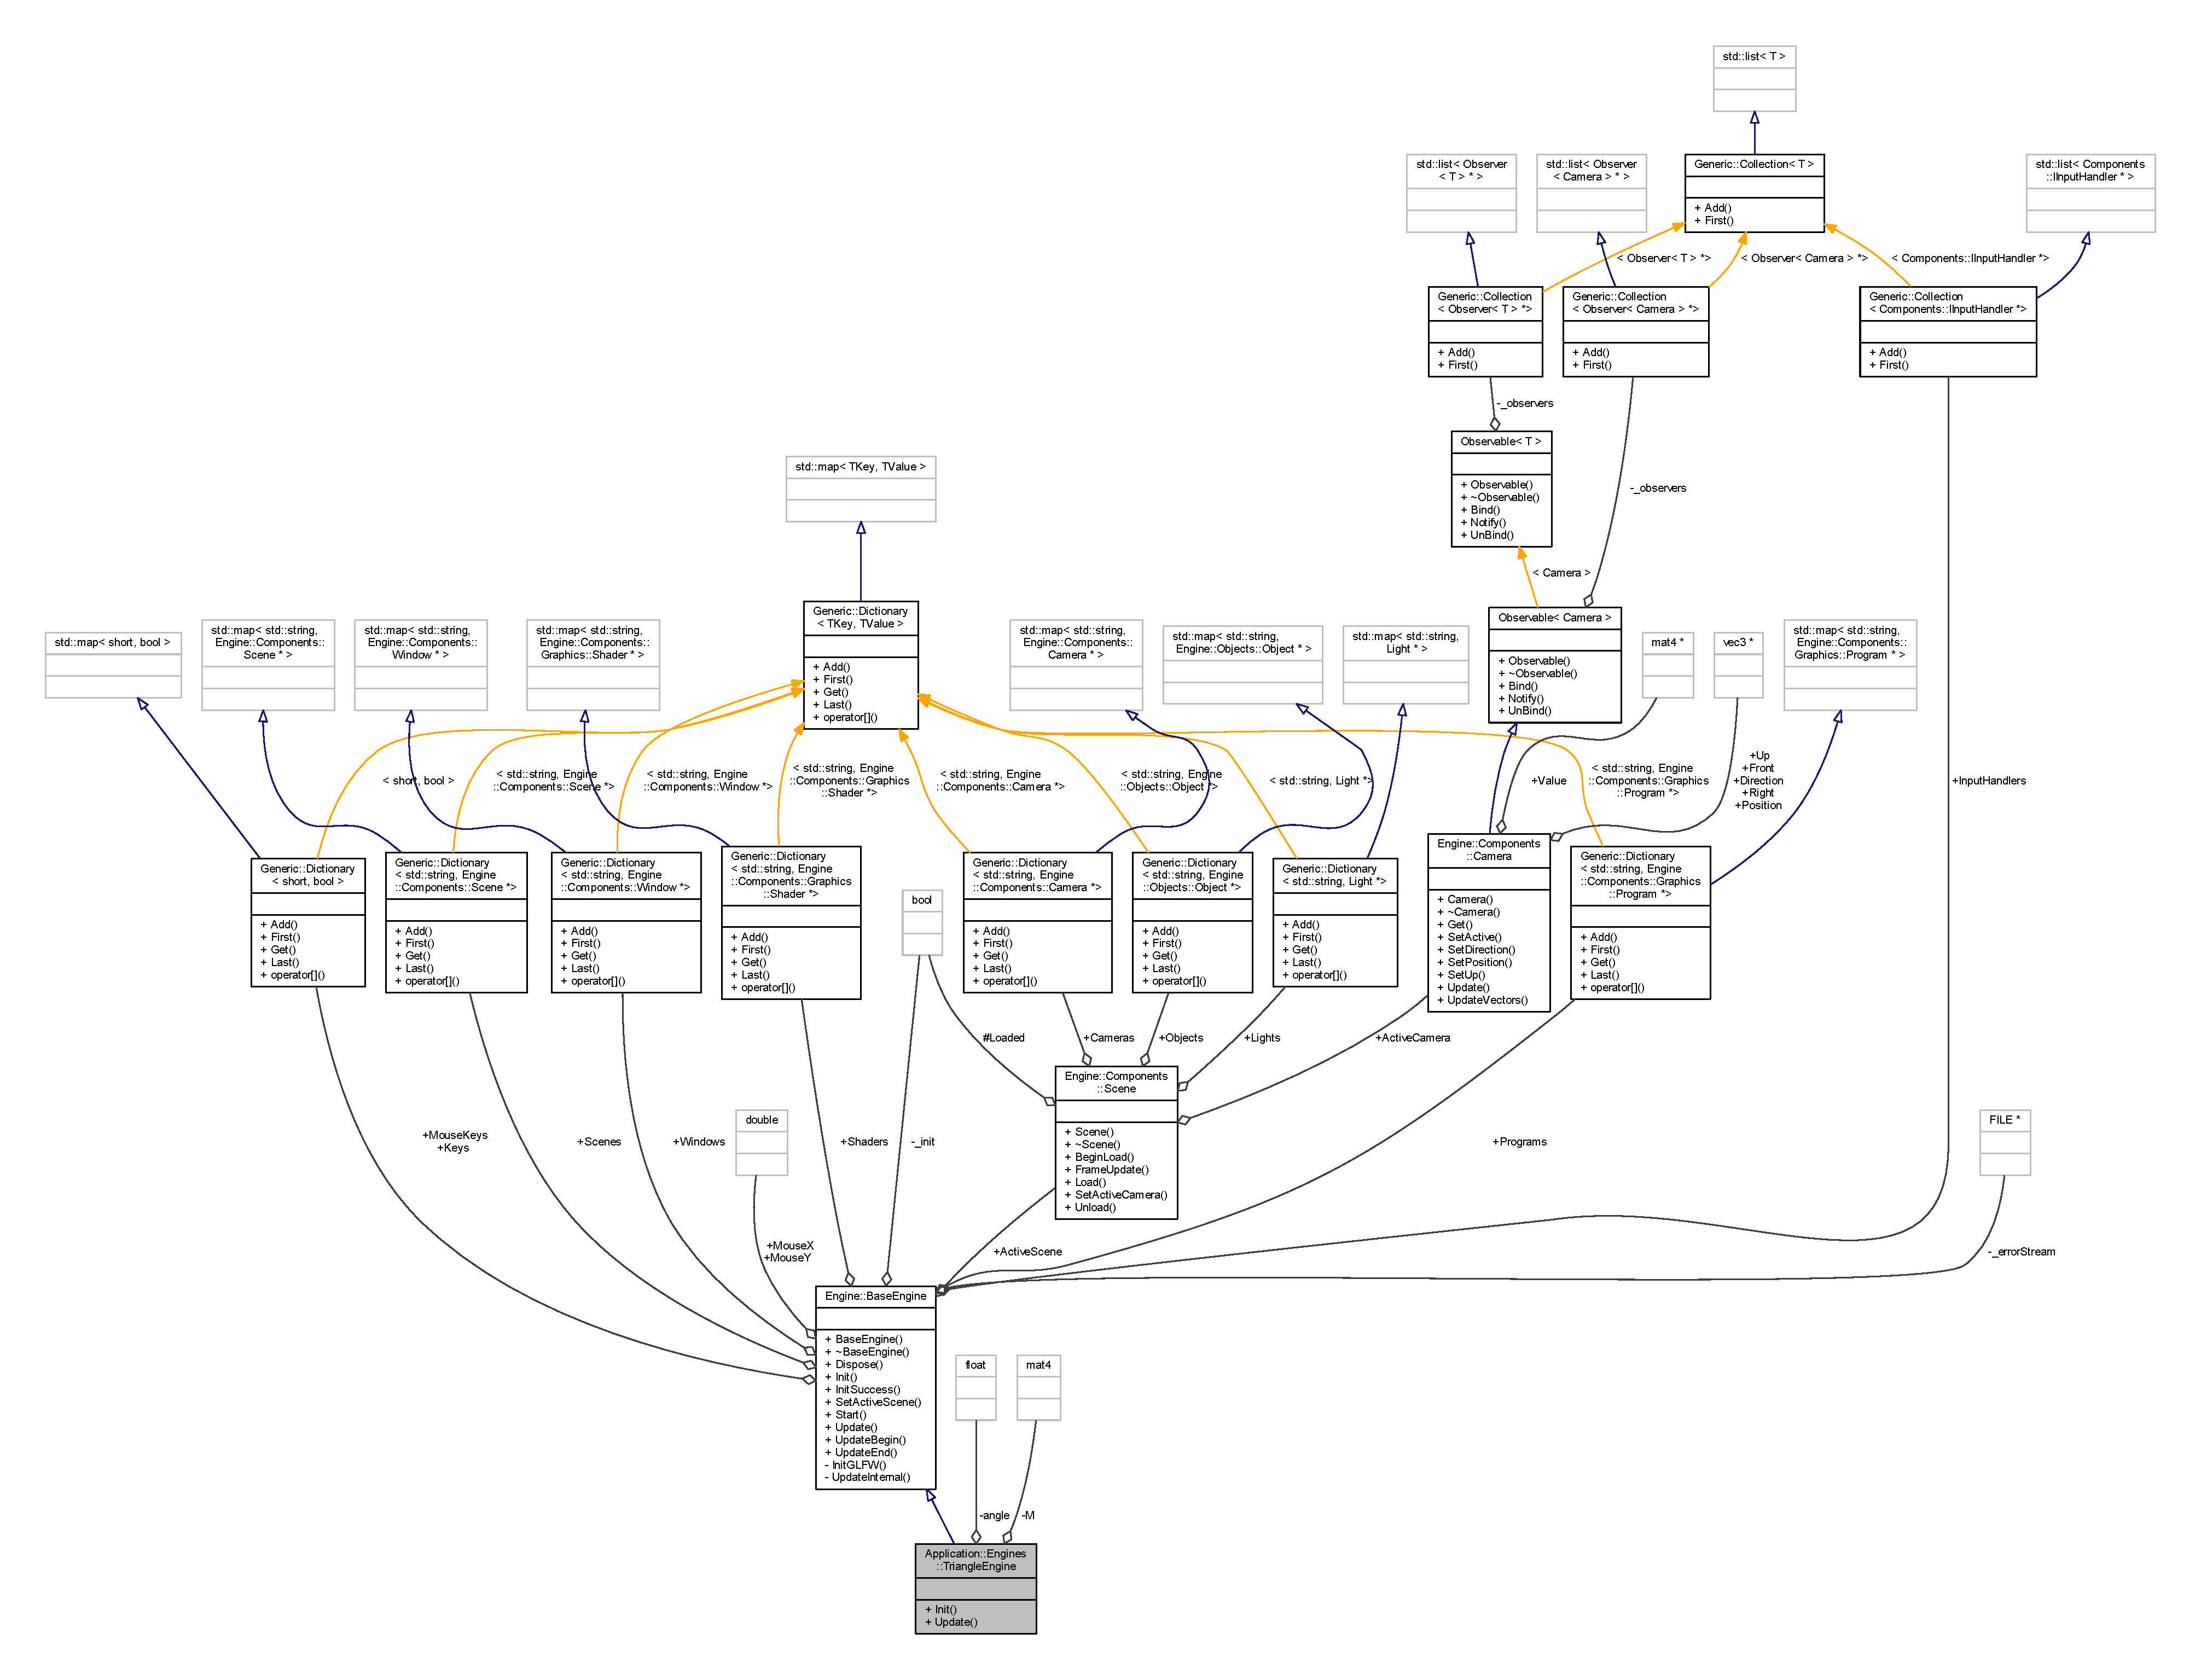
\includegraphics[width=350pt]{classApplication_1_1Engines_1_1TriangleEngine__coll__graph}
\end{center}
\end{figure}
\subsection*{Public Member Functions}
\begin{DoxyCompactItemize}
\item 
\mbox{\hyperlink{classEngine_1_1BaseEngine_ad838c97afe1790cb35527f0b58e81e6b}{Base\+Engine}} $\ast$ \mbox{\hyperlink{classEngine_1_1BaseEngine_acd5cd5d2189d24e038b23477b7dce405}{Dispose}} ()
\item 
\mbox{\hyperlink{classApplication_1_1Engines_1_1TriangleEngine}{Triangle\+Engine}} $\ast$ \mbox{\hyperlink{classApplication_1_1Engines_1_1TriangleEngine_a4fc68c683c3beaadf7d41f36627d3492}{Init}} (std\+::\+F\+I\+LE $\ast$error\+Stream=stderr) override
\item 
bool \mbox{\hyperlink{classEngine_1_1BaseEngine_a7a1c9b833049b3eb61194cab113dfe89}{Init\+Success}} ()
\item 
virtual void \mbox{\hyperlink{classEngine_1_1BaseEngine_afc82c6a00d5a9d4714740fc5eab5db86}{Set\+Active\+Scene}} (Components\+::\+Scene $\ast$scene=nullptr)
\item 
virtual void \mbox{\hyperlink{classEngine_1_1BaseEngine_a525fdc7a1da7eecb514ad5763f06be79}{Start}} ()
\item 
void \mbox{\hyperlink{classApplication_1_1Engines_1_1TriangleEngine_a0578bee716800df84d59f13c291bc6d0}{Update}} (\+::\mbox{\hyperlink{classEngine_1_1Components_1_1Window}{Engine\+::\+Components\+::\+Window}} $\ast$window) override
\item 
virtual void \mbox{\hyperlink{classEngine_1_1BaseEngine_a01c23c2073f08939a660f3b7a866852c}{Update}} (Components\+::\+Window $\ast$window)
\item 
virtual void \mbox{\hyperlink{classEngine_1_1BaseEngine_aace6be2a42d12b64fbd35f1acdb08408}{Update\+Begin}} (Components\+::\+Window $\ast$window)
\item 
virtual void \mbox{\hyperlink{classEngine_1_1BaseEngine_a7c07c98e583df042a0eb01e0ddec85a1}{Update\+End}} (Components\+::\+Window $\ast$window)
\end{DoxyCompactItemize}
\subsection*{Public Attributes}
\begin{DoxyCompactItemize}
\item 
Components\+::\+Scene $\ast$ \mbox{\hyperlink{classEngine_1_1BaseEngine_adb3dbc839da9d821e08b18d8a221698d}{Active\+Scene}}
\item 
\mbox{\hyperlink{classGeneric_1_1Collection}{Generic\+::\+Collection}}$<$ Components\+::\+I\+Input\+Handler $\ast$ $>$ $\ast$ \mbox{\hyperlink{classEngine_1_1BaseEngine_a134fa082c5a64d62b76ddf926647e7cc}{Input\+Handlers}}
\item 
\mbox{\hyperlink{classGeneric_1_1Dictionary}{Generic\+::\+Dictionary}}$<$ short, bool $>$ \mbox{\hyperlink{classEngine_1_1BaseEngine_a65321a97e83f0a6ee90df3efac2d3307}{Keys}}
\item 
\mbox{\hyperlink{classGeneric_1_1Dictionary}{Generic\+::\+Dictionary}}$<$ short, bool $>$ \mbox{\hyperlink{classEngine_1_1BaseEngine_a3ee2bdddb66d45b8c808ffd937ba9c50}{Mouse\+Keys}}
\item 
double \mbox{\hyperlink{classEngine_1_1BaseEngine_a5fe085152ebe93346900407f6b41a034}{MouseX}}
\item 
double \mbox{\hyperlink{classEngine_1_1BaseEngine_a143c9c32dbbdc70bf1546ffe275bf384}{MouseY}}
\item 
\mbox{\hyperlink{classGeneric_1_1Dictionary}{Generic\+::\+Dictionary}}$<$ std\+::string, Components\+::\+Graphics\+::\+Program $\ast$ $>$ $\ast$ \mbox{\hyperlink{classEngine_1_1BaseEngine_ae0f86360ea3a384caefe443dd8f88601}{Programs}}
\item 
\mbox{\hyperlink{classGeneric_1_1Dictionary}{Generic\+::\+Dictionary}}$<$ std\+::string, Components\+::\+Scene $\ast$ $>$ $\ast$ \mbox{\hyperlink{classEngine_1_1BaseEngine_afd02af3c2fbe9bb734db014dec06585a}{Scenes}}
\item 
\mbox{\hyperlink{classGeneric_1_1Dictionary}{Generic\+::\+Dictionary}}$<$ std\+::string, Components\+::\+Graphics\+::\+Shader $\ast$ $>$ $\ast$ \mbox{\hyperlink{classEngine_1_1BaseEngine_a2582dee3f73da82bb422b43317b85e3b}{Shaders}}
\item 
\mbox{\hyperlink{classGeneric_1_1Dictionary}{Generic\+::\+Dictionary}}$<$ std\+::string, Components\+::\+Window $\ast$ $>$ $\ast$ \mbox{\hyperlink{classEngine_1_1BaseEngine_a4a1a4c4dae052e66ecc4f326eeed4d33}{Windows}}
\end{DoxyCompactItemize}
\subsection*{Private Attributes}
\begin{DoxyCompactItemize}
\item 
float \mbox{\hyperlink{classApplication_1_1Engines_1_1TriangleEngine_a71526be47b8a14b2f9980fa3ff1022b2}{angle}}
\item 
glm\+::mat4 \mbox{\hyperlink{classApplication_1_1Engines_1_1TriangleEngine_a12ea2b98b8900cccf469e0bf0ea89316}{M}}
\end{DoxyCompactItemize}


\subsection{Detailed Description}


Definition at line 8 of file Triangle\+Engine.\+h.



\subsection{Member Function Documentation}
\mbox{\Hypertarget{classEngine_1_1BaseEngine_acd5cd5d2189d24e038b23477b7dce405}\label{classEngine_1_1BaseEngine_acd5cd5d2189d24e038b23477b7dce405}} 
\index{Application\+::\+Engines\+::\+Triangle\+Engine@{Application\+::\+Engines\+::\+Triangle\+Engine}!Dispose@{Dispose}}
\index{Dispose@{Dispose}!Application\+::\+Engines\+::\+Triangle\+Engine@{Application\+::\+Engines\+::\+Triangle\+Engine}}
\subsubsection{\texorpdfstring{Dispose()}{Dispose()}}
{\footnotesize\ttfamily \mbox{\hyperlink{classEngine_1_1BaseEngine}{Engine\+::\+Base\+Engine}} $\ast$ Engine\+::\+Base\+Engine\+::\+Dispose (\begin{DoxyParamCaption}{ }\end{DoxyParamCaption})\hspace{0.3cm}{\ttfamily [inherited]}}



Definition at line 51 of file Base\+Engine.\+cpp.


\begin{DoxyCode}
52 \{
53     glfwTerminate();
54     \textcolor{keywordflow}{return} \textcolor{keyword}{this};
55 \}
\end{DoxyCode}
\mbox{\Hypertarget{classApplication_1_1Engines_1_1TriangleEngine_a4fc68c683c3beaadf7d41f36627d3492}\label{classApplication_1_1Engines_1_1TriangleEngine_a4fc68c683c3beaadf7d41f36627d3492}} 
\index{Application\+::\+Engines\+::\+Triangle\+Engine@{Application\+::\+Engines\+::\+Triangle\+Engine}!Init@{Init}}
\index{Init@{Init}!Application\+::\+Engines\+::\+Triangle\+Engine@{Application\+::\+Engines\+::\+Triangle\+Engine}}
\subsubsection{\texorpdfstring{Init()}{Init()}}
{\footnotesize\ttfamily \mbox{\hyperlink{classApplication_1_1Engines_1_1TriangleEngine}{Application\+::\+Engines\+::\+Triangle\+Engine}} $\ast$ Application\+::\+Engines\+::\+Triangle\+Engine\+::\+Init (\begin{DoxyParamCaption}\item[{std\+::\+F\+I\+LE $\ast$}]{error\+Stream = {\ttfamily stderr} }\end{DoxyParamCaption})\hspace{0.3cm}{\ttfamily [override]}, {\ttfamily [virtual]}}



Reimplemented from \mbox{\hyperlink{classEngine_1_1BaseEngine_ad9c141fe48c8c91e14e77ed5fcb90196}{Engine\+::\+Base\+Engine}}.



Definition at line 7 of file Triangle\+Engine.\+cpp.



References angle, fragment\+\_\+shader, M, Engine\+::\+Base\+Engine\+::\+Programs, Engine\+::\+Base\+Engine\+::\+Scenes, Engine\+::\+Base\+Engine\+::\+Set\+Active\+Scene(), Engine\+::\+Base\+Engine\+::\+Shaders, vertex\+\_\+shader, and Engine\+::\+Base\+Engine\+::\+Windows.


\begin{DoxyCode}
8 \{
9     BaseEngine::Init(errorStream);
10 
11     \textcolor{keyword}{const} \textcolor{keywordtype}{char}* \mbox{\hyperlink{ZPGEngine_8cpp_afc33b8912f9f93d1d2544df04ad4a81a}{vertex\_shader}} =
12         \textcolor{stringliteral}{"#version 330\(\backslash\)n"}
13         \textcolor{stringliteral}{"uniform mat4 modelMatrix;"}
14         \textcolor{stringliteral}{"layout(location=0) in vec3 vp;"}
15         \textcolor{stringliteral}{"layout(location=1) in vec3 vertNormal;"}
16         \textcolor{stringliteral}{"void main () \{"}
17         \textcolor{stringliteral}{" gl\_Position = modelMatrix * vec4 (vp, 1.0);"}
18         \textcolor{stringliteral}{"\}"};
19 
20     \textcolor{keyword}{const} \textcolor{keywordtype}{char}*  \mbox{\hyperlink{ZPGEngine_8cpp_ab187f2ba2a2f72ea5571921a1a856582}{fragment\_shader}} =
21         \textcolor{stringliteral}{"#version 330\(\backslash\)n"}
22         \textcolor{stringliteral}{"uniform float color;"}
23         \textcolor{stringliteral}{"out vec4 frag\_colour;"}
24         \textcolor{stringliteral}{"void main () \{"}
25         \textcolor{stringliteral}{"     frag\_colour = vec4 (color, 1.0-color, 0.0, 1.0);"}
26         \textcolor{stringliteral}{"\}"};
27 
28     \mbox{\hyperlink{classEngine_1_1BaseEngine_a4a1a4c4dae052e66ecc4f326eeed4d33}{Windows}}->Add(\textcolor{stringliteral}{"zpg"}, (new ::Engine::Components::Window(800, 600, \textcolor{stringliteral}{"ZPG - Triangle"}, 100.0f))
29         ->Show()
30         ->Info(std::cout)
31     );
32 
33 
34     \mbox{\hyperlink{classEngine_1_1BaseEngine_a2582dee3f73da82bb422b43317b85e3b}{Shaders}}->Add(\textcolor{stringliteral}{"vertex"}, \textcolor{keyword}{new} \mbox{\hyperlink{classEngine_1_1Components_1_1Graphics_1_1Shader}{Engine::Components::Graphics::Shader}}
      (GL\_VERTEX\_SHADER, \mbox{\hyperlink{ZPGEngine_8cpp_afc33b8912f9f93d1d2544df04ad4a81a}{vertex\_shader}}));
35     \mbox{\hyperlink{classEngine_1_1BaseEngine_a2582dee3f73da82bb422b43317b85e3b}{Shaders}}->Add(\textcolor{stringliteral}{"fragment"}, \textcolor{keyword}{new} \mbox{\hyperlink{classEngine_1_1Components_1_1Graphics_1_1Shader}{Engine::Components::Graphics::Shader}}
      (GL\_FRAGMENT\_SHADER, \mbox{\hyperlink{ZPGEngine_8cpp_ab187f2ba2a2f72ea5571921a1a856582}{fragment\_shader}}));
36 
37     \mbox{\hyperlink{classEngine_1_1BaseEngine_ae0f86360ea3a384caefe443dd8f88601}{Programs}}->Add(\textcolor{stringliteral}{"basic"}, (\textcolor{keyword}{new} \mbox{\hyperlink{classEngine_1_1Components_1_1Graphics_1_1Program}{Engine::Components::Graphics::Program}}
      ())->AddShaders(\mbox{\hyperlink{classEngine_1_1BaseEngine_a2582dee3f73da82bb422b43317b85e3b}{Shaders}}));
38 
39     \mbox{\hyperlink{classEngine_1_1BaseEngine_afd02af3c2fbe9bb734db014dec06585a}{Scenes}}->Add(\textcolor{stringliteral}{"triangle"}, \textcolor{keyword}{new} Scenes::TriangleScene());
40     \mbox{\hyperlink{classEngine_1_1BaseEngine_afd02af3c2fbe9bb734db014dec06585a}{Scenes}}->Add(\textcolor{stringliteral}{"sphere"}, \textcolor{keyword}{new} Scenes::SphereScene());
41 
42     \textcolor{comment}{//SetActiveScene(Scenes->Get("triangle"));}
43     \mbox{\hyperlink{classEngine_1_1BaseEngine_afc82c6a00d5a9d4714740fc5eab5db86}{SetActiveScene}}(\mbox{\hyperlink{classEngine_1_1BaseEngine_afd02af3c2fbe9bb734db014dec06585a}{Scenes}}->Get(\textcolor{stringliteral}{"sphere"}));
44 
45     \mbox{\hyperlink{classApplication_1_1Engines_1_1TriangleEngine_a12ea2b98b8900cccf469e0bf0ea89316}{M}} = glm::mat4(1.0f);
46     \mbox{\hyperlink{classApplication_1_1Engines_1_1TriangleEngine_a71526be47b8a14b2f9980fa3ff1022b2}{angle}} = 0.0f;
47     \textcolor{keywordflow}{return} \textcolor{keyword}{this};
48 \}
\end{DoxyCode}
Here is the call graph for this function\+:
\nopagebreak
\begin{figure}[H]
\begin{center}
\leavevmode
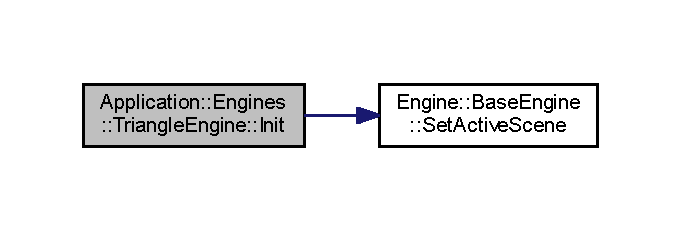
\includegraphics[width=327pt]{classApplication_1_1Engines_1_1TriangleEngine_a4fc68c683c3beaadf7d41f36627d3492_cgraph}
\end{center}
\end{figure}
\mbox{\Hypertarget{classEngine_1_1BaseEngine_a7a1c9b833049b3eb61194cab113dfe89}\label{classEngine_1_1BaseEngine_a7a1c9b833049b3eb61194cab113dfe89}} 
\index{Application\+::\+Engines\+::\+Triangle\+Engine@{Application\+::\+Engines\+::\+Triangle\+Engine}!Init\+Success@{Init\+Success}}
\index{Init\+Success@{Init\+Success}!Application\+::\+Engines\+::\+Triangle\+Engine@{Application\+::\+Engines\+::\+Triangle\+Engine}}
\subsubsection{\texorpdfstring{Init\+Success()}{InitSuccess()}}
{\footnotesize\ttfamily bool Engine\+::\+Base\+Engine\+::\+Init\+Success (\begin{DoxyParamCaption}{ }\end{DoxyParamCaption})\hspace{0.3cm}{\ttfamily [inherited]}}



Definition at line 46 of file Base\+Engine.\+cpp.


\begin{DoxyCode}
47 \{
48     \textcolor{keywordflow}{return} \mbox{\hyperlink{classEngine_1_1BaseEngine_a79e265845b321c0e9822fb170c564e55}{\_init}};
49 \}
\end{DoxyCode}
\mbox{\Hypertarget{classEngine_1_1BaseEngine_afc82c6a00d5a9d4714740fc5eab5db86}\label{classEngine_1_1BaseEngine_afc82c6a00d5a9d4714740fc5eab5db86}} 
\index{Application\+::\+Engines\+::\+Triangle\+Engine@{Application\+::\+Engines\+::\+Triangle\+Engine}!Set\+Active\+Scene@{Set\+Active\+Scene}}
\index{Set\+Active\+Scene@{Set\+Active\+Scene}!Application\+::\+Engines\+::\+Triangle\+Engine@{Application\+::\+Engines\+::\+Triangle\+Engine}}
\subsubsection{\texorpdfstring{Set\+Active\+Scene()}{SetActiveScene()}}
{\footnotesize\ttfamily void Engine\+::\+Base\+Engine\+::\+Set\+Active\+Scene (\begin{DoxyParamCaption}\item[{\mbox{\hyperlink{classEngine_1_1Components_1_1Scene}{Components\+::\+Scene}} $\ast$}]{scene = {\ttfamily nullptr} }\end{DoxyParamCaption})\hspace{0.3cm}{\ttfamily [virtual]}, {\ttfamily [inherited]}}



Definition at line 132 of file Base\+Engine.\+cpp.



Referenced by Application\+::\+Engines\+::\+Basic\+Engine\+::\+Init(), Application\+::\+Engines\+::\+Z\+P\+G\+Engine\+::\+Init(), Application\+::\+Engines\+::\+Camera\+Engine\+::\+Init(), Init(), and Application\+::\+Engines\+::\+Light\+Engine\+::\+Init().


\begin{DoxyCode}
133 \{
134     \textcolor{keywordflow}{if} (scene == \textcolor{keyword}{nullptr} && !\mbox{\hyperlink{classEngine_1_1BaseEngine_afd02af3c2fbe9bb734db014dec06585a}{Scenes}}->empty())
135         \mbox{\hyperlink{classEngine_1_1BaseEngine_adb3dbc839da9d821e08b18d8a221698d}{ActiveScene}} = \mbox{\hyperlink{classEngine_1_1BaseEngine_afd02af3c2fbe9bb734db014dec06585a}{Scenes}}->begin()->second;
136     \textcolor{keywordflow}{else}
137         \mbox{\hyperlink{classEngine_1_1BaseEngine_adb3dbc839da9d821e08b18d8a221698d}{ActiveScene}} = scene;     
138 \}
\end{DoxyCode}
Here is the caller graph for this function\+:
\nopagebreak
\begin{figure}[H]
\begin{center}
\leavevmode
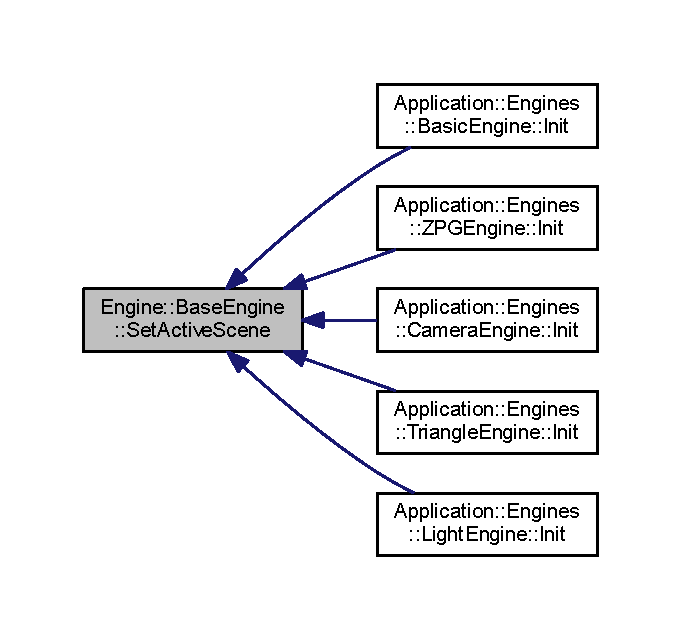
\includegraphics[width=327pt]{classEngine_1_1BaseEngine_afc82c6a00d5a9d4714740fc5eab5db86_icgraph}
\end{center}
\end{figure}
\mbox{\Hypertarget{classEngine_1_1BaseEngine_a525fdc7a1da7eecb514ad5763f06be79}\label{classEngine_1_1BaseEngine_a525fdc7a1da7eecb514ad5763f06be79}} 
\index{Application\+::\+Engines\+::\+Triangle\+Engine@{Application\+::\+Engines\+::\+Triangle\+Engine}!Start@{Start}}
\index{Start@{Start}!Application\+::\+Engines\+::\+Triangle\+Engine@{Application\+::\+Engines\+::\+Triangle\+Engine}}
\subsubsection{\texorpdfstring{Start()}{Start()}}
{\footnotesize\ttfamily void Engine\+::\+Base\+Engine\+::\+Start (\begin{DoxyParamCaption}{ }\end{DoxyParamCaption})\hspace{0.3cm}{\ttfamily [virtual]}, {\ttfamily [inherited]}}



Definition at line 126 of file Base\+Engine.\+cpp.



Referenced by main().


\begin{DoxyCode}
127 \{
128     system(\textcolor{stringliteral}{"cls"});
129     \mbox{\hyperlink{classEngine_1_1BaseEngine_aad3c237ca657b9f22f76fccf7fc7561f}{UpdateInternal}}();
130 \}
\end{DoxyCode}
Here is the caller graph for this function\+:
\nopagebreak
\begin{figure}[H]
\begin{center}
\leavevmode
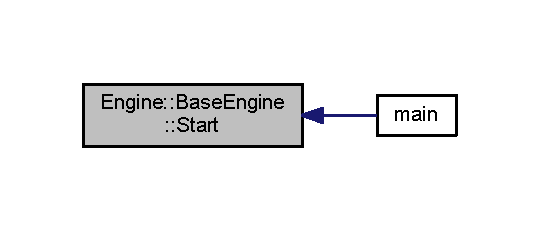
\includegraphics[width=259pt]{classEngine_1_1BaseEngine_a525fdc7a1da7eecb514ad5763f06be79_icgraph}
\end{center}
\end{figure}
\mbox{\Hypertarget{classApplication_1_1Engines_1_1TriangleEngine_a0578bee716800df84d59f13c291bc6d0}\label{classApplication_1_1Engines_1_1TriangleEngine_a0578bee716800df84d59f13c291bc6d0}} 
\index{Application\+::\+Engines\+::\+Triangle\+Engine@{Application\+::\+Engines\+::\+Triangle\+Engine}!Update@{Update}}
\index{Update@{Update}!Application\+::\+Engines\+::\+Triangle\+Engine@{Application\+::\+Engines\+::\+Triangle\+Engine}}
\subsubsection{\texorpdfstring{Update()}{Update()}\hspace{0.1cm}{\footnotesize\ttfamily [1/2]}}
{\footnotesize\ttfamily void Application\+::\+Engines\+::\+Triangle\+Engine\+::\+Update (\begin{DoxyParamCaption}\item[{\+::\mbox{\hyperlink{classEngine_1_1Components_1_1Window}{Engine\+::\+Components\+::\+Window}} $\ast$}]{window }\end{DoxyParamCaption})\hspace{0.3cm}{\ttfamily [override]}}



Definition at line 50 of file Triangle\+Engine.\+cpp.


\begin{DoxyCode}
51 \{
52     \textcolor{keywordflow}{if}(\mbox{\hyperlink{classEngine_1_1BaseEngine_adb3dbc839da9d821e08b18d8a221698d}{ActiveScene}} != \textcolor{keyword}{nullptr} && \mbox{\hyperlink{classEngine_1_1BaseEngine_adb3dbc839da9d821e08b18d8a221698d}{ActiveScene}}->\mbox{\hyperlink{classEngine_1_1Components_1_1Scene_a23481feabaaa56bf5613765db03af4da}{Objects}} != \textcolor{keyword}{nullptr} && !
      \mbox{\hyperlink{classEngine_1_1BaseEngine_adb3dbc839da9d821e08b18d8a221698d}{ActiveScene}}->\mbox{\hyperlink{classEngine_1_1Components_1_1Scene_a23481feabaaa56bf5613765db03af4da}{Objects}}->empty())
53     \textcolor{keywordflow}{for} (\textcolor{keyword}{auto}& it : *\mbox{\hyperlink{classEngine_1_1BaseEngine_adb3dbc839da9d821e08b18d8a221698d}{ActiveScene}}->\mbox{\hyperlink{classEngine_1_1Components_1_1Scene_a23481feabaaa56bf5613765db03af4da}{Objects}})
54     \{
55         std::cout << \textcolor{stringliteral}{"Object: "} << it.first << std::endl;
56         \textcolor{keyword}{auto} \textcolor{keywordtype}{object} = it.second;
57         \textcolor{keywordtype}{object}->Draw();
58         \mbox{\hyperlink{classApplication_1_1Engines_1_1TriangleEngine_a71526be47b8a14b2f9980fa3ff1022b2}{angle}} += 0.1f;
59     \}
60 \}
\end{DoxyCode}
\mbox{\Hypertarget{classEngine_1_1BaseEngine_a01c23c2073f08939a660f3b7a866852c}\label{classEngine_1_1BaseEngine_a01c23c2073f08939a660f3b7a866852c}} 
\index{Application\+::\+Engines\+::\+Triangle\+Engine@{Application\+::\+Engines\+::\+Triangle\+Engine}!Update@{Update}}
\index{Update@{Update}!Application\+::\+Engines\+::\+Triangle\+Engine@{Application\+::\+Engines\+::\+Triangle\+Engine}}
\subsubsection{\texorpdfstring{Update()}{Update()}\hspace{0.1cm}{\footnotesize\ttfamily [2/2]}}
{\footnotesize\ttfamily void Engine\+::\+Base\+Engine\+::\+Update (\begin{DoxyParamCaption}\item[{\mbox{\hyperlink{classEngine_1_1Components_1_1Window}{Components\+::\+Window}} $\ast$}]{window }\end{DoxyParamCaption})\hspace{0.3cm}{\ttfamily [virtual]}, {\ttfamily [inherited]}}



Definition at line 112 of file Base\+Engine.\+cpp.


\begin{DoxyCode}
113 \{
114 \}
\end{DoxyCode}
\mbox{\Hypertarget{classEngine_1_1BaseEngine_aace6be2a42d12b64fbd35f1acdb08408}\label{classEngine_1_1BaseEngine_aace6be2a42d12b64fbd35f1acdb08408}} 
\index{Application\+::\+Engines\+::\+Triangle\+Engine@{Application\+::\+Engines\+::\+Triangle\+Engine}!Update\+Begin@{Update\+Begin}}
\index{Update\+Begin@{Update\+Begin}!Application\+::\+Engines\+::\+Triangle\+Engine@{Application\+::\+Engines\+::\+Triangle\+Engine}}
\subsubsection{\texorpdfstring{Update\+Begin()}{UpdateBegin()}}
{\footnotesize\ttfamily void Engine\+::\+Base\+Engine\+::\+Update\+Begin (\begin{DoxyParamCaption}\item[{\mbox{\hyperlink{classEngine_1_1Components_1_1Window}{Components\+::\+Window}} $\ast$}]{window }\end{DoxyParamCaption})\hspace{0.3cm}{\ttfamily [virtual]}, {\ttfamily [inherited]}}



Definition at line 57 of file Base\+Engine.\+cpp.



References Engine\+::\+Components\+::\+Window\+::\+Get().


\begin{DoxyCode}
58 \{
59     \textcolor{comment}{// Scene}
60     \mbox{\hyperlink{classEngine_1_1BaseEngine_adb3dbc839da9d821e08b18d8a221698d}{ActiveScene}}->\mbox{\hyperlink{classEngine_1_1Components_1_1Scene_af18bd334fe66952b8d79b8e9e99ab2d8}{BeginLoad}}(\textcolor{keyword}{this});
61 
62     \textcolor{comment}{// Buffers}
63     glEnable(GL\_DEPTH\_TEST);
64     glDepthFunc(GL\_LESS);
65     glClear(GL\_COLOR\_BUFFER\_BIT | GL\_DEPTH\_BUFFER\_BIT);
66 
67     \textcolor{comment}{// Input}
68     \textcolor{keywordtype}{short} mouseKeysActive = 0;
69     glfwGetCursorPos(window->Get(), &\mbox{\hyperlink{classEngine_1_1BaseEngine_a5fe085152ebe93346900407f6b41a034}{MouseX}}, &\mbox{\hyperlink{classEngine_1_1BaseEngine_a143c9c32dbbdc70bf1546ffe275bf384}{MouseY}});
70     \textcolor{keywordflow}{for}(\textcolor{keywordtype}{short} i = 0; i < 8; i++)
71     \{
72         \textcolor{keyword}{const} \textcolor{keywordtype}{int} state = glfwGetMouseButton(window->Get(), i);
73         \textcolor{keyword}{auto} value = \mbox{\hyperlink{classEngine_1_1BaseEngine_a3ee2bdddb66d45b8c808ffd937ba9c50}{MouseKeys}}[i];
74         \textcolor{comment}{// flip state}
75         \textcolor{keywordflow}{if} (state == GLFW\_PRESS && !value)
76             \mbox{\hyperlink{classEngine_1_1BaseEngine_a3ee2bdddb66d45b8c808ffd937ba9c50}{MouseKeys}}.\mbox{\hyperlink{classGeneric_1_1Dictionary_ae7cb006f801b21c172e8fbac8794fa99}{Add}}(i, \textcolor{keyword}{true});
77         \textcolor{keywordflow}{else} \textcolor{keywordflow}{if} (state == GLFW\_RELEASE && value)
78             \mbox{\hyperlink{classEngine_1_1BaseEngine_a3ee2bdddb66d45b8c808ffd937ba9c50}{MouseKeys}}.\mbox{\hyperlink{classGeneric_1_1Dictionary_ae7cb006f801b21c172e8fbac8794fa99}{Add}}(i, \textcolor{keyword}{false});
79         \textcolor{keywordflow}{if} (\mbox{\hyperlink{classEngine_1_1BaseEngine_a3ee2bdddb66d45b8c808ffd937ba9c50}{MouseKeys}}[i])
80             mouseKeysActive++;
81     \}
82     \textcolor{keywordtype}{short} keysActive = 0;
83     SetConsoleCursorPosition(GetStdHandle(STD\_OUTPUT\_HANDLE), \{ 40, keysActive \});
84     fprintf(\mbox{\hyperlink{classEngine_1_1BaseEngine_a26fd54a1ee2733f9c654af5afcfa96cf}{\_errorStream}}, \textcolor{stringliteral}{"                           "});
85     \textcolor{keywordflow}{for} (\textcolor{keywordtype}{short} i = 1; i < 512; i++)
86     \{
87         \textcolor{keyword}{const} \textcolor{keywordtype}{int} state = glfwGetKey(window->Get(), i);
88         \textcolor{keyword}{auto} value = \mbox{\hyperlink{classEngine_1_1BaseEngine_a65321a97e83f0a6ee90df3efac2d3307}{Keys}}[i];
89         \textcolor{comment}{// flip state}
90         \textcolor{keywordflow}{if} (state == GLFW\_PRESS && !value)
91             \mbox{\hyperlink{classEngine_1_1BaseEngine_a65321a97e83f0a6ee90df3efac2d3307}{Keys}}.\mbox{\hyperlink{classGeneric_1_1Dictionary_ae7cb006f801b21c172e8fbac8794fa99}{Add}}(i, \textcolor{keyword}{true});
92         \textcolor{keywordflow}{else} \textcolor{keywordflow}{if} (state == GLFW\_RELEASE && value)
93             \mbox{\hyperlink{classEngine_1_1BaseEngine_a65321a97e83f0a6ee90df3efac2d3307}{Keys}}.\mbox{\hyperlink{classGeneric_1_1Dictionary_ae7cb006f801b21c172e8fbac8794fa99}{Add}}(i, \textcolor{keyword}{false});
94         \textcolor{keywordflow}{if} (\mbox{\hyperlink{classEngine_1_1BaseEngine_a65321a97e83f0a6ee90df3efac2d3307}{Keys}}[i])
95             keysActive++;
96     \}
97     \textcolor{keywordtype}{bool} handleKeys = \textcolor{keyword}{true},
98          handleMouse = \textcolor{keyword}{true};
99     \textcolor{keywordflow}{for} (\textcolor{keyword}{auto} handler : *\mbox{\hyperlink{classEngine_1_1BaseEngine_a134fa082c5a64d62b76ddf926647e7cc}{InputHandlers}})
100     \{
101         \textcolor{keywordflow}{if}(handleKeys)
102             handleKeys = handler->HandleKeys(\textcolor{keyword}{this}, window, \mbox{\hyperlink{classEngine_1_1BaseEngine_adb3dbc839da9d821e08b18d8a221698d}{ActiveScene}}, 
      \mbox{\hyperlink{classEngine_1_1BaseEngine_a65321a97e83f0a6ee90df3efac2d3307}{Keys}}, keysActive);
103         \textcolor{keywordflow}{if}(handleMouse)
104             handleMouse = handler->HandleMouse(\textcolor{keyword}{this}, window, \mbox{\hyperlink{classEngine_1_1BaseEngine_adb3dbc839da9d821e08b18d8a221698d}{ActiveScene}}, 
      \mbox{\hyperlink{classEngine_1_1BaseEngine_a5fe085152ebe93346900407f6b41a034}{MouseX}}, \mbox{\hyperlink{classEngine_1_1BaseEngine_a143c9c32dbbdc70bf1546ffe275bf384}{MouseY}}, \mbox{\hyperlink{classEngine_1_1BaseEngine_a3ee2bdddb66d45b8c808ffd937ba9c50}{MouseKeys}}, mouseKeysActive);
105         \textcolor{keywordflow}{if}(!handleKeys && !handleMouse)
106             \textcolor{keywordflow}{break};
107     \}
108 
109     SetConsoleCursorPosition(GetStdHandle(STD\_OUTPUT\_HANDLE), \{ 0,0 \});
110 \}
\end{DoxyCode}
Here is the call graph for this function\+:
\nopagebreak
\begin{figure}[H]
\begin{center}
\leavevmode
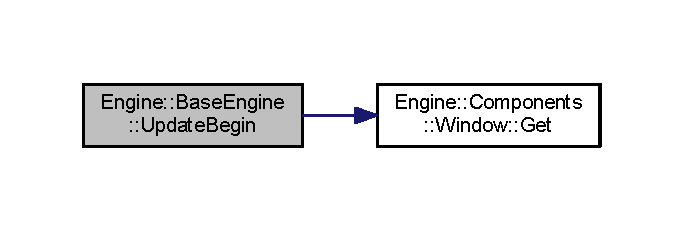
\includegraphics[width=328pt]{classEngine_1_1BaseEngine_aace6be2a42d12b64fbd35f1acdb08408_cgraph}
\end{center}
\end{figure}
\mbox{\Hypertarget{classEngine_1_1BaseEngine_a7c07c98e583df042a0eb01e0ddec85a1}\label{classEngine_1_1BaseEngine_a7c07c98e583df042a0eb01e0ddec85a1}} 
\index{Application\+::\+Engines\+::\+Triangle\+Engine@{Application\+::\+Engines\+::\+Triangle\+Engine}!Update\+End@{Update\+End}}
\index{Update\+End@{Update\+End}!Application\+::\+Engines\+::\+Triangle\+Engine@{Application\+::\+Engines\+::\+Triangle\+Engine}}
\subsubsection{\texorpdfstring{Update\+End()}{UpdateEnd()}}
{\footnotesize\ttfamily void Engine\+::\+Base\+Engine\+::\+Update\+End (\begin{DoxyParamCaption}\item[{\mbox{\hyperlink{classEngine_1_1Components_1_1Window}{Components\+::\+Window}} $\ast$}]{window }\end{DoxyParamCaption})\hspace{0.3cm}{\ttfamily [virtual]}, {\ttfamily [inherited]}}



Definition at line 116 of file Base\+Engine.\+cpp.



References Engine\+::\+Components\+::\+Window\+::\+Get().


\begin{DoxyCode}
117 \{
118     \textcolor{comment}{// update other events like input handling}
119     glfwPollEvents();
120     \textcolor{comment}{// put the stuff we’ve been drawing onto the display}
121     glfwSwapBuffers(window->Get());
122 
123     \mbox{\hyperlink{classEngine_1_1BaseEngine_adb3dbc839da9d821e08b18d8a221698d}{ActiveScene}}->\mbox{\hyperlink{classEngine_1_1Components_1_1Scene_abd8fcdcac52dbce6a0a18de3860ab087}{FrameUpdate}}(\textcolor{keyword}{this});
124 \}
\end{DoxyCode}
Here is the call graph for this function\+:
\nopagebreak
\begin{figure}[H]
\begin{center}
\leavevmode
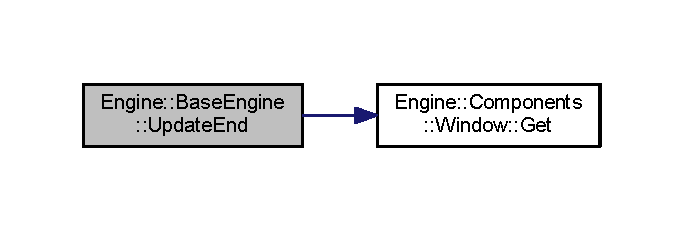
\includegraphics[width=328pt]{classEngine_1_1BaseEngine_a7c07c98e583df042a0eb01e0ddec85a1_cgraph}
\end{center}
\end{figure}


\subsection{Member Data Documentation}
\mbox{\Hypertarget{classEngine_1_1BaseEngine_adb3dbc839da9d821e08b18d8a221698d}\label{classEngine_1_1BaseEngine_adb3dbc839da9d821e08b18d8a221698d}} 
\index{Application\+::\+Engines\+::\+Triangle\+Engine@{Application\+::\+Engines\+::\+Triangle\+Engine}!Active\+Scene@{Active\+Scene}}
\index{Active\+Scene@{Active\+Scene}!Application\+::\+Engines\+::\+Triangle\+Engine@{Application\+::\+Engines\+::\+Triangle\+Engine}}
\subsubsection{\texorpdfstring{Active\+Scene}{ActiveScene}}
{\footnotesize\ttfamily Components\+::\+Scene$\ast$ Engine\+::\+Base\+Engine\+::\+Active\+Scene\hspace{0.3cm}{\ttfamily [inherited]}}



Definition at line 34 of file Base\+Engine.\+h.



Referenced by Engine\+::\+Base\+Engine\+::\+Base\+Engine(), Application\+::\+Engines\+::\+Camera\+Engine\+::\+Init(), and Application\+::\+Engines\+::\+Light\+Engine\+::\+Init().

\mbox{\Hypertarget{classApplication_1_1Engines_1_1TriangleEngine_a71526be47b8a14b2f9980fa3ff1022b2}\label{classApplication_1_1Engines_1_1TriangleEngine_a71526be47b8a14b2f9980fa3ff1022b2}} 
\index{Application\+::\+Engines\+::\+Triangle\+Engine@{Application\+::\+Engines\+::\+Triangle\+Engine}!angle@{angle}}
\index{angle@{angle}!Application\+::\+Engines\+::\+Triangle\+Engine@{Application\+::\+Engines\+::\+Triangle\+Engine}}
\subsubsection{\texorpdfstring{angle}{angle}}
{\footnotesize\ttfamily float Application\+::\+Engines\+::\+Triangle\+Engine\+::angle\hspace{0.3cm}{\ttfamily [private]}}



Definition at line 15 of file Triangle\+Engine.\+h.



Referenced by Init().

\mbox{\Hypertarget{classEngine_1_1BaseEngine_a134fa082c5a64d62b76ddf926647e7cc}\label{classEngine_1_1BaseEngine_a134fa082c5a64d62b76ddf926647e7cc}} 
\index{Application\+::\+Engines\+::\+Triangle\+Engine@{Application\+::\+Engines\+::\+Triangle\+Engine}!Input\+Handlers@{Input\+Handlers}}
\index{Input\+Handlers@{Input\+Handlers}!Application\+::\+Engines\+::\+Triangle\+Engine@{Application\+::\+Engines\+::\+Triangle\+Engine}}
\subsubsection{\texorpdfstring{Input\+Handlers}{InputHandlers}}
{\footnotesize\ttfamily \mbox{\hyperlink{classGeneric_1_1Collection}{Generic\+::\+Collection}}$<$Components\+::\+I\+Input\+Handler$\ast$$>$$\ast$ Engine\+::\+Base\+Engine\+::\+Input\+Handlers\hspace{0.3cm}{\ttfamily [inherited]}}



Definition at line 31 of file Base\+Engine.\+h.



Referenced by Engine\+::\+Base\+Engine\+::\+Base\+Engine(), and Application\+::\+Engines\+::\+Light\+Engine\+::\+Init().

\mbox{\Hypertarget{classEngine_1_1BaseEngine_a65321a97e83f0a6ee90df3efac2d3307}\label{classEngine_1_1BaseEngine_a65321a97e83f0a6ee90df3efac2d3307}} 
\index{Application\+::\+Engines\+::\+Triangle\+Engine@{Application\+::\+Engines\+::\+Triangle\+Engine}!Keys@{Keys}}
\index{Keys@{Keys}!Application\+::\+Engines\+::\+Triangle\+Engine@{Application\+::\+Engines\+::\+Triangle\+Engine}}
\subsubsection{\texorpdfstring{Keys}{Keys}}
{\footnotesize\ttfamily \mbox{\hyperlink{classGeneric_1_1Dictionary}{Generic\+::\+Dictionary}}$<$short, bool$>$ Engine\+::\+Base\+Engine\+::\+Keys\hspace{0.3cm}{\ttfamily [inherited]}}



Definition at line 32 of file Base\+Engine.\+h.



Referenced by Engine\+::\+Base\+Engine\+::\+Base\+Engine().

\mbox{\Hypertarget{classApplication_1_1Engines_1_1TriangleEngine_a12ea2b98b8900cccf469e0bf0ea89316}\label{classApplication_1_1Engines_1_1TriangleEngine_a12ea2b98b8900cccf469e0bf0ea89316}} 
\index{Application\+::\+Engines\+::\+Triangle\+Engine@{Application\+::\+Engines\+::\+Triangle\+Engine}!M@{M}}
\index{M@{M}!Application\+::\+Engines\+::\+Triangle\+Engine@{Application\+::\+Engines\+::\+Triangle\+Engine}}
\subsubsection{\texorpdfstring{M}{M}}
{\footnotesize\ttfamily glm\+::mat4 Application\+::\+Engines\+::\+Triangle\+Engine\+::M\hspace{0.3cm}{\ttfamily [private]}}



Definition at line 14 of file Triangle\+Engine.\+h.



Referenced by Init().

\mbox{\Hypertarget{classEngine_1_1BaseEngine_a3ee2bdddb66d45b8c808ffd937ba9c50}\label{classEngine_1_1BaseEngine_a3ee2bdddb66d45b8c808ffd937ba9c50}} 
\index{Application\+::\+Engines\+::\+Triangle\+Engine@{Application\+::\+Engines\+::\+Triangle\+Engine}!Mouse\+Keys@{Mouse\+Keys}}
\index{Mouse\+Keys@{Mouse\+Keys}!Application\+::\+Engines\+::\+Triangle\+Engine@{Application\+::\+Engines\+::\+Triangle\+Engine}}
\subsubsection{\texorpdfstring{Mouse\+Keys}{MouseKeys}}
{\footnotesize\ttfamily \mbox{\hyperlink{classGeneric_1_1Dictionary}{Generic\+::\+Dictionary}}$<$short, bool$>$ Engine\+::\+Base\+Engine\+::\+Mouse\+Keys\hspace{0.3cm}{\ttfamily [inherited]}}



Definition at line 33 of file Base\+Engine.\+h.



Referenced by Engine\+::\+Base\+Engine\+::\+Base\+Engine().

\mbox{\Hypertarget{classEngine_1_1BaseEngine_a5fe085152ebe93346900407f6b41a034}\label{classEngine_1_1BaseEngine_a5fe085152ebe93346900407f6b41a034}} 
\index{Application\+::\+Engines\+::\+Triangle\+Engine@{Application\+::\+Engines\+::\+Triangle\+Engine}!MouseX@{MouseX}}
\index{MouseX@{MouseX}!Application\+::\+Engines\+::\+Triangle\+Engine@{Application\+::\+Engines\+::\+Triangle\+Engine}}
\subsubsection{\texorpdfstring{MouseX}{MouseX}}
{\footnotesize\ttfamily double Engine\+::\+Base\+Engine\+::\+MouseX\hspace{0.3cm}{\ttfamily [inherited]}}



Definition at line 35 of file Base\+Engine.\+h.

\mbox{\Hypertarget{classEngine_1_1BaseEngine_a143c9c32dbbdc70bf1546ffe275bf384}\label{classEngine_1_1BaseEngine_a143c9c32dbbdc70bf1546ffe275bf384}} 
\index{Application\+::\+Engines\+::\+Triangle\+Engine@{Application\+::\+Engines\+::\+Triangle\+Engine}!MouseY@{MouseY}}
\index{MouseY@{MouseY}!Application\+::\+Engines\+::\+Triangle\+Engine@{Application\+::\+Engines\+::\+Triangle\+Engine}}
\subsubsection{\texorpdfstring{MouseY}{MouseY}}
{\footnotesize\ttfamily double Engine\+::\+Base\+Engine\+::\+MouseY\hspace{0.3cm}{\ttfamily [inherited]}}



Definition at line 36 of file Base\+Engine.\+h.

\mbox{\Hypertarget{classEngine_1_1BaseEngine_ae0f86360ea3a384caefe443dd8f88601}\label{classEngine_1_1BaseEngine_ae0f86360ea3a384caefe443dd8f88601}} 
\index{Application\+::\+Engines\+::\+Triangle\+Engine@{Application\+::\+Engines\+::\+Triangle\+Engine}!Programs@{Programs}}
\index{Programs@{Programs}!Application\+::\+Engines\+::\+Triangle\+Engine@{Application\+::\+Engines\+::\+Triangle\+Engine}}
\subsubsection{\texorpdfstring{Programs}{Programs}}
{\footnotesize\ttfamily \mbox{\hyperlink{classGeneric_1_1Dictionary}{Generic\+::\+Dictionary}}$<$std\+::string, Components\+::\+Graphics\+::\+Program$\ast$$>$$\ast$ Engine\+::\+Base\+Engine\+::\+Programs\hspace{0.3cm}{\ttfamily [inherited]}}



Definition at line 28 of file Base\+Engine.\+h.



Referenced by Engine\+::\+Base\+Engine\+::\+Base\+Engine(), Application\+::\+Input\+::\+Handlers\+::\+Camera\+Input\+Handler\+::\+Handle\+Mouse(), Application\+::\+Engines\+::\+Camera\+Engine\+::\+Init(), Application\+::\+Engines\+::\+Z\+P\+G\+Engine\+::\+Init(), Init(), Application\+::\+Engines\+::\+Basic\+Engine\+::\+Init(), Application\+::\+Engines\+::\+Light\+Engine\+::\+Init(), Application\+::\+Scenes\+::\+Triangle\+Scene\+::\+Load(), and Application\+::\+Scenes\+::\+Sphere\+Scene\+::\+Load().

\mbox{\Hypertarget{classEngine_1_1BaseEngine_afd02af3c2fbe9bb734db014dec06585a}\label{classEngine_1_1BaseEngine_afd02af3c2fbe9bb734db014dec06585a}} 
\index{Application\+::\+Engines\+::\+Triangle\+Engine@{Application\+::\+Engines\+::\+Triangle\+Engine}!Scenes@{Scenes}}
\index{Scenes@{Scenes}!Application\+::\+Engines\+::\+Triangle\+Engine@{Application\+::\+Engines\+::\+Triangle\+Engine}}
\subsubsection{\texorpdfstring{Scenes}{Scenes}}
{\footnotesize\ttfamily \mbox{\hyperlink{classGeneric_1_1Dictionary}{Generic\+::\+Dictionary}}$<$std\+::string, Components\+::\+Scene$\ast$$>$$\ast$ Engine\+::\+Base\+Engine\+::\+Scenes\hspace{0.3cm}{\ttfamily [inherited]}}



Definition at line 30 of file Base\+Engine.\+h.



Referenced by Engine\+::\+Base\+Engine\+::\+Base\+Engine(), Application\+::\+Engines\+::\+Z\+P\+G\+Engine\+::\+Init(), Application\+::\+Engines\+::\+Camera\+Engine\+::\+Init(), Application\+::\+Engines\+::\+Basic\+Engine\+::\+Init(), Init(), and Application\+::\+Engines\+::\+Light\+Engine\+::\+Init().

\mbox{\Hypertarget{classEngine_1_1BaseEngine_a2582dee3f73da82bb422b43317b85e3b}\label{classEngine_1_1BaseEngine_a2582dee3f73da82bb422b43317b85e3b}} 
\index{Application\+::\+Engines\+::\+Triangle\+Engine@{Application\+::\+Engines\+::\+Triangle\+Engine}!Shaders@{Shaders}}
\index{Shaders@{Shaders}!Application\+::\+Engines\+::\+Triangle\+Engine@{Application\+::\+Engines\+::\+Triangle\+Engine}}
\subsubsection{\texorpdfstring{Shaders}{Shaders}}
{\footnotesize\ttfamily \mbox{\hyperlink{classGeneric_1_1Dictionary}{Generic\+::\+Dictionary}}$<$std\+::string, Components\+::\+Graphics\+::\+Shader$\ast$$>$$\ast$ Engine\+::\+Base\+Engine\+::\+Shaders\hspace{0.3cm}{\ttfamily [inherited]}}



Definition at line 29 of file Base\+Engine.\+h.



Referenced by Engine\+::\+Base\+Engine\+::\+Base\+Engine(), Application\+::\+Input\+::\+Handlers\+::\+Camera\+Input\+Handler\+::\+Handle\+Mouse(), Application\+::\+Engines\+::\+Camera\+Engine\+::\+Init(), Application\+::\+Engines\+::\+Basic\+Engine\+::\+Init(), Application\+::\+Engines\+::\+Z\+P\+G\+Engine\+::\+Init(), Init(), and Application\+::\+Engines\+::\+Light\+Engine\+::\+Init().

\mbox{\Hypertarget{classEngine_1_1BaseEngine_a4a1a4c4dae052e66ecc4f326eeed4d33}\label{classEngine_1_1BaseEngine_a4a1a4c4dae052e66ecc4f326eeed4d33}} 
\index{Application\+::\+Engines\+::\+Triangle\+Engine@{Application\+::\+Engines\+::\+Triangle\+Engine}!Windows@{Windows}}
\index{Windows@{Windows}!Application\+::\+Engines\+::\+Triangle\+Engine@{Application\+::\+Engines\+::\+Triangle\+Engine}}
\subsubsection{\texorpdfstring{Windows}{Windows}}
{\footnotesize\ttfamily \mbox{\hyperlink{classGeneric_1_1Dictionary}{Generic\+::\+Dictionary}}$<$std\+::string, Components\+::\+Window$\ast$$>$$\ast$ Engine\+::\+Base\+Engine\+::\+Windows\hspace{0.3cm}{\ttfamily [inherited]}}



Definition at line 27 of file Base\+Engine.\+h.



Referenced by Engine\+::\+Base\+Engine\+::\+Base\+Engine(), Application\+::\+Engines\+::\+Z\+P\+G\+Engine\+::\+Init(), Application\+::\+Engines\+::\+Camera\+Engine\+::\+Init(), Application\+::\+Engines\+::\+Basic\+Engine\+::\+Init(), Init(), and Application\+::\+Engines\+::\+Light\+Engine\+::\+Init().



The documentation for this class was generated from the following files\+:\begin{DoxyCompactItemize}
\item 
Z\+P\+G/\mbox{\hyperlink{TriangleEngine_8h}{Triangle\+Engine.\+h}}\item 
Z\+P\+G/\mbox{\hyperlink{TriangleEngine_8cpp}{Triangle\+Engine.\+cpp}}\end{DoxyCompactItemize}

\hypertarget{classApplication_1_1Engines_1_1ZPGEngine}{}\section{Application\+:\+:Engines\+:\+:Z\+P\+G\+Engine Class Reference}
\label{classApplication_1_1Engines_1_1ZPGEngine}\index{Application\+::\+Engines\+::\+Z\+P\+G\+Engine@{Application\+::\+Engines\+::\+Z\+P\+G\+Engine}}


{\ttfamily \#include $<$Z\+P\+G\+Engine.\+h$>$}



Inheritance diagram for Application\+:\+:Engines\+:\+:Z\+P\+G\+Engine\+:
\nopagebreak
\begin{figure}[H]
\begin{center}
\leavevmode
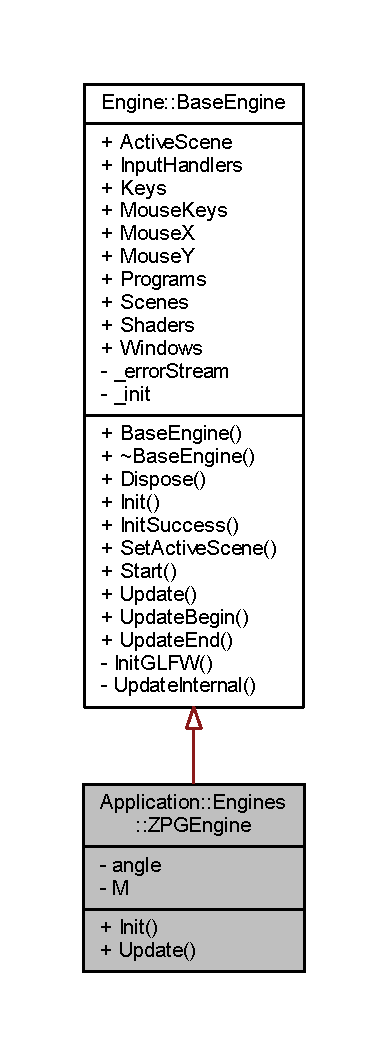
\includegraphics[width=186pt]{classApplication_1_1Engines_1_1ZPGEngine__inherit__graph}
\end{center}
\end{figure}


Collaboration diagram for Application\+:\+:Engines\+:\+:Z\+P\+G\+Engine\+:
\nopagebreak
\begin{figure}[H]
\begin{center}
\leavevmode
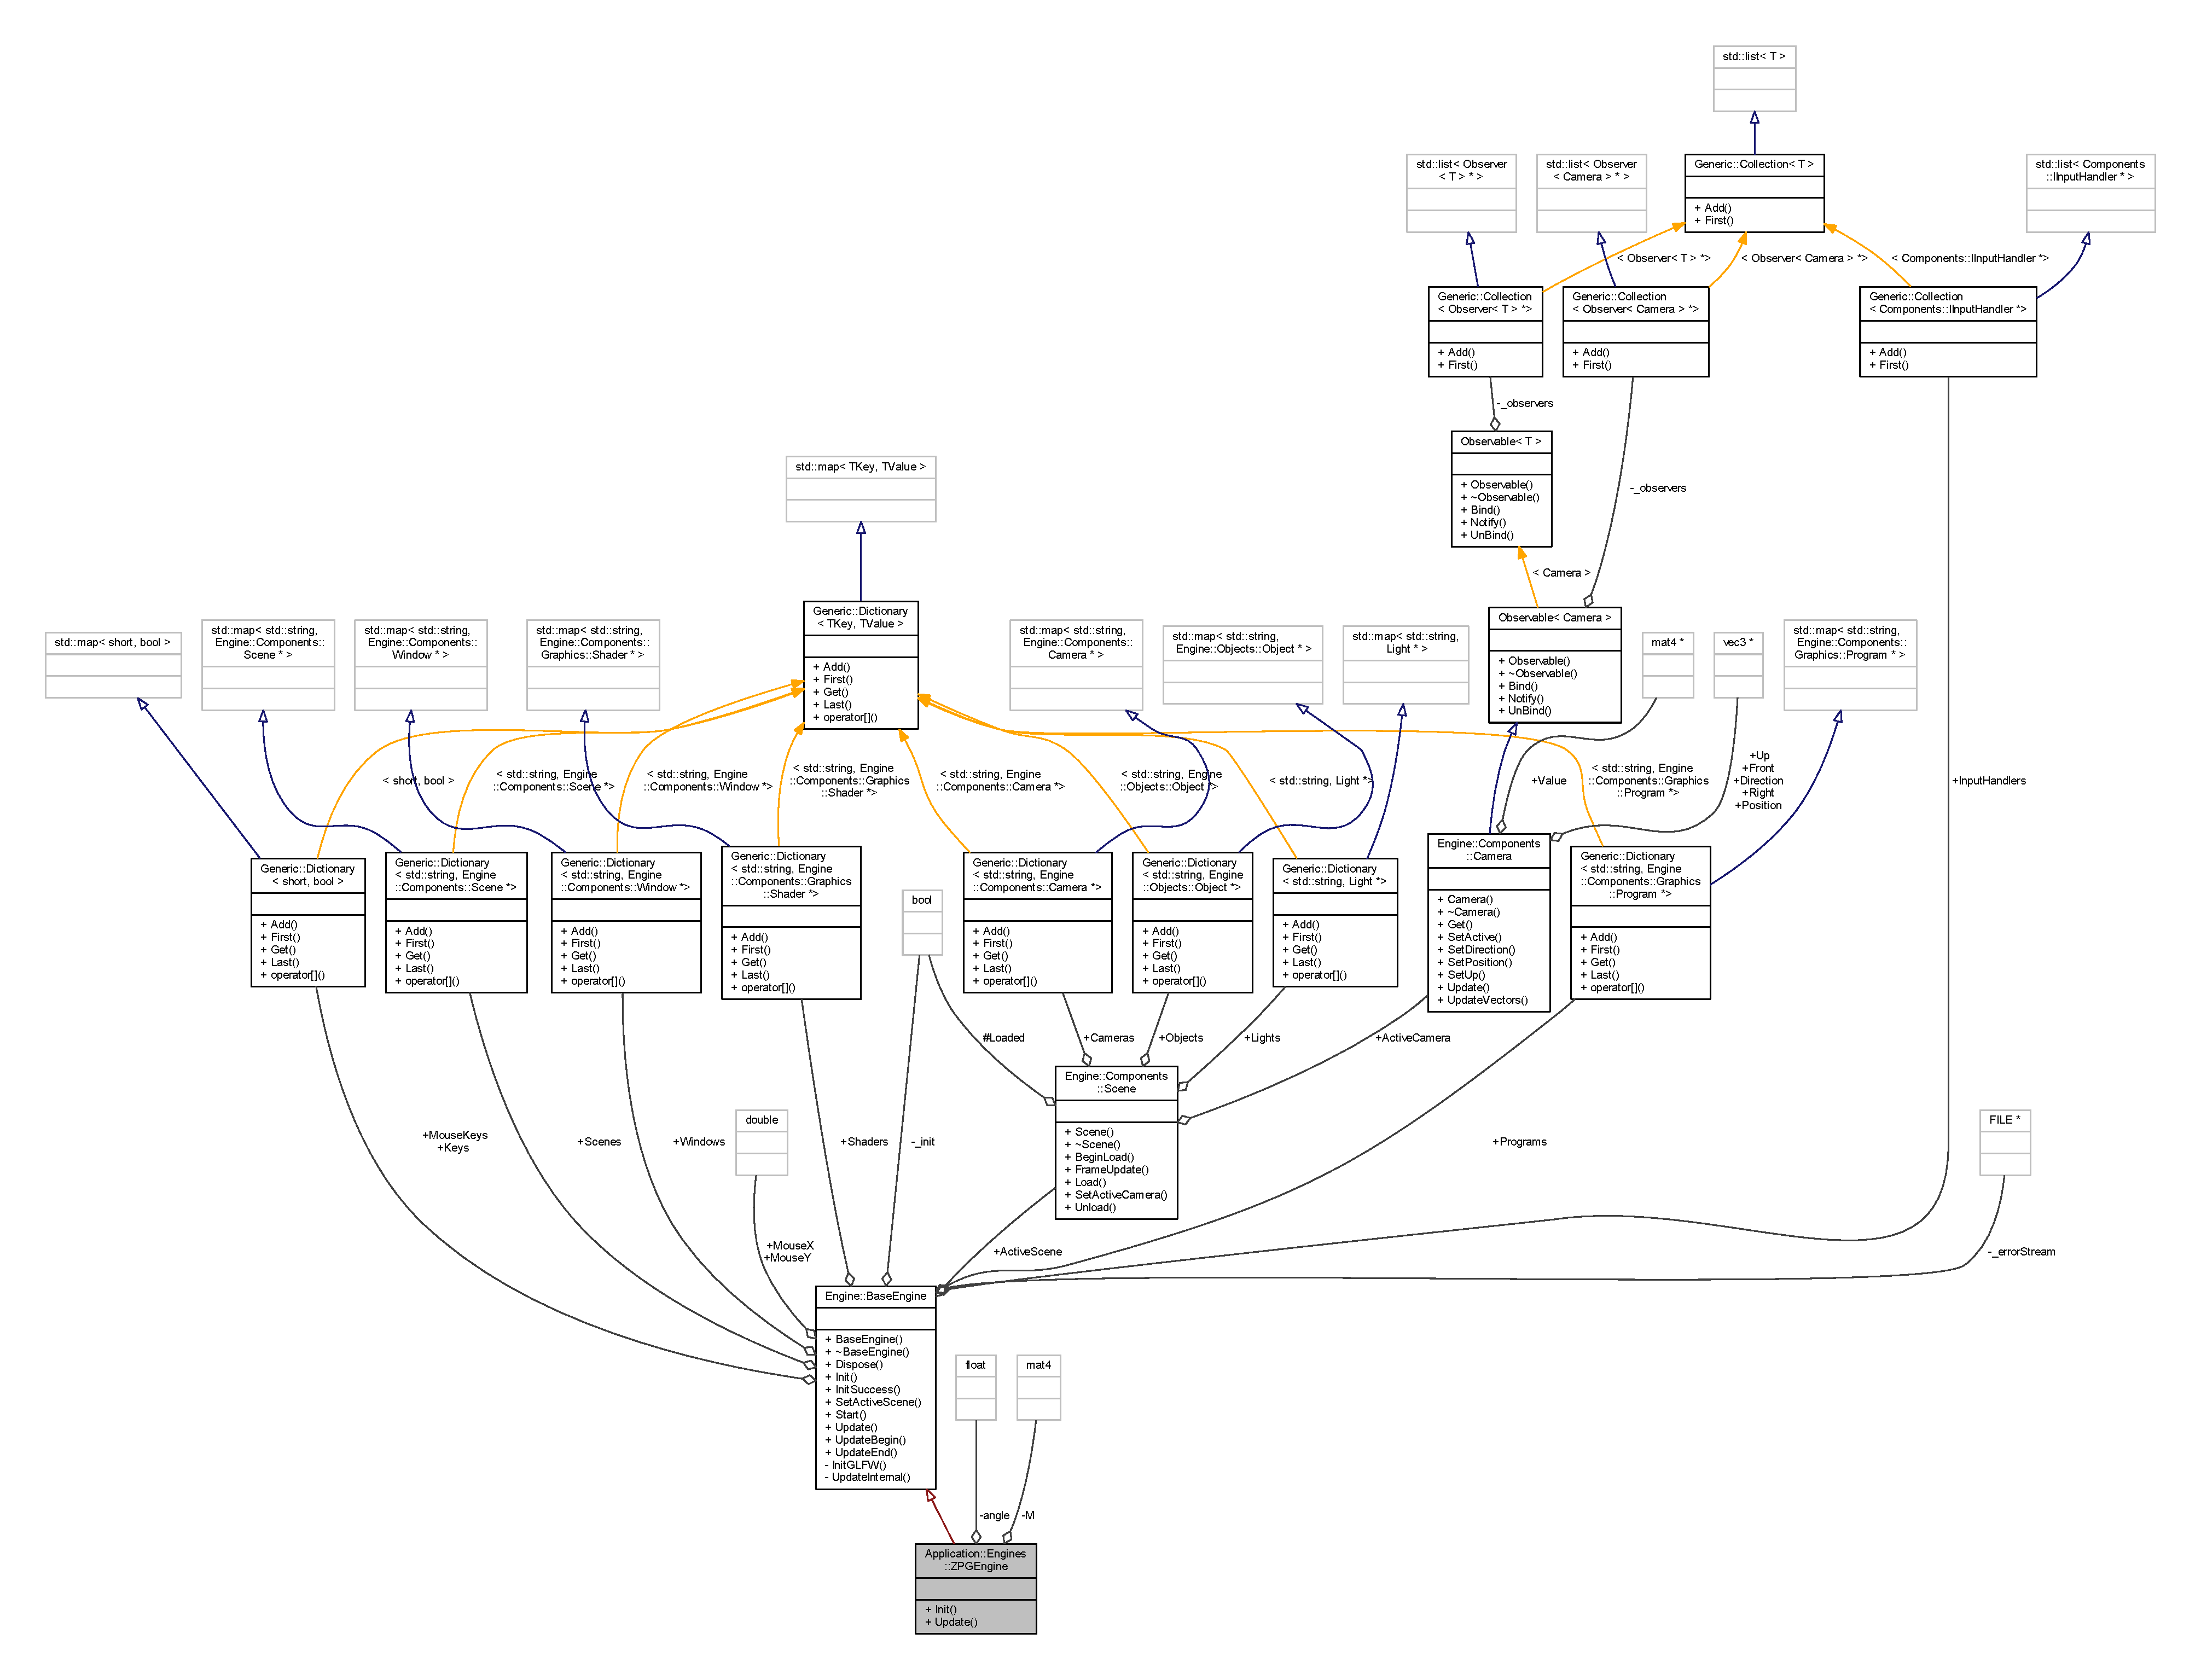
\includegraphics[width=350pt]{classApplication_1_1Engines_1_1ZPGEngine__coll__graph}
\end{center}
\end{figure}
\subsection*{Public Member Functions}
\begin{DoxyCompactItemize}
\item 
\mbox{\hyperlink{classApplication_1_1Engines_1_1ZPGEngine}{Z\+P\+G\+Engine}} $\ast$ \mbox{\hyperlink{classApplication_1_1Engines_1_1ZPGEngine_a08a065a6200bf4465b71efa08f173cc5}{Init}} (std\+::\+F\+I\+LE $\ast$error\+Stream=stderr) override
\item 
void \mbox{\hyperlink{classApplication_1_1Engines_1_1ZPGEngine_a44b3d077ad688846aaa40d95ad14f851}{Update}} (\+::\mbox{\hyperlink{classEngine_1_1Components_1_1Window}{Engine\+::\+Components\+::\+Window}} $\ast$window) override
\end{DoxyCompactItemize}
\subsection*{Private Member Functions}
\begin{DoxyCompactItemize}
\item 
\mbox{\hyperlink{classEngine_1_1BaseEngine_ad838c97afe1790cb35527f0b58e81e6b}{Base\+Engine}} $\ast$ \mbox{\hyperlink{classEngine_1_1BaseEngine_acd5cd5d2189d24e038b23477b7dce405}{Dispose}} ()
\item 
bool \mbox{\hyperlink{classEngine_1_1BaseEngine_a7a1c9b833049b3eb61194cab113dfe89}{Init\+Success}} ()
\item 
virtual void \mbox{\hyperlink{classEngine_1_1BaseEngine_afc82c6a00d5a9d4714740fc5eab5db86}{Set\+Active\+Scene}} (Components\+::\+Scene $\ast$scene=nullptr)
\item 
virtual void \mbox{\hyperlink{classEngine_1_1BaseEngine_a525fdc7a1da7eecb514ad5763f06be79}{Start}} ()
\item 
virtual void \mbox{\hyperlink{classEngine_1_1BaseEngine_a01c23c2073f08939a660f3b7a866852c}{Update}} (Components\+::\+Window $\ast$window)
\item 
virtual void \mbox{\hyperlink{classEngine_1_1BaseEngine_aace6be2a42d12b64fbd35f1acdb08408}{Update\+Begin}} (Components\+::\+Window $\ast$window)
\item 
virtual void \mbox{\hyperlink{classEngine_1_1BaseEngine_a7c07c98e583df042a0eb01e0ddec85a1}{Update\+End}} (Components\+::\+Window $\ast$window)
\end{DoxyCompactItemize}
\subsection*{Private Attributes}
\begin{DoxyCompactItemize}
\item 
Components\+::\+Scene $\ast$ \mbox{\hyperlink{classEngine_1_1BaseEngine_adb3dbc839da9d821e08b18d8a221698d}{Active\+Scene}}
\item 
float \mbox{\hyperlink{classApplication_1_1Engines_1_1ZPGEngine_adee8aa02ea2c15751eb6222bded1f729}{angle}}
\item 
\mbox{\hyperlink{classGeneric_1_1Collection}{Generic\+::\+Collection}}$<$ Components\+::\+I\+Input\+Handler $\ast$ $>$ $\ast$ \mbox{\hyperlink{classEngine_1_1BaseEngine_a134fa082c5a64d62b76ddf926647e7cc}{Input\+Handlers}}
\item 
\mbox{\hyperlink{classGeneric_1_1Dictionary}{Generic\+::\+Dictionary}}$<$ short, bool $>$ \mbox{\hyperlink{classEngine_1_1BaseEngine_a65321a97e83f0a6ee90df3efac2d3307}{Keys}}
\item 
glm\+::mat4 \mbox{\hyperlink{classApplication_1_1Engines_1_1ZPGEngine_a6e982d6b97e8d538cdf8df9a7f4c6cd0}{M}}
\item 
\mbox{\hyperlink{classGeneric_1_1Dictionary}{Generic\+::\+Dictionary}}$<$ short, bool $>$ \mbox{\hyperlink{classEngine_1_1BaseEngine_a3ee2bdddb66d45b8c808ffd937ba9c50}{Mouse\+Keys}}
\item 
double \mbox{\hyperlink{classEngine_1_1BaseEngine_a5fe085152ebe93346900407f6b41a034}{MouseX}}
\item 
double \mbox{\hyperlink{classEngine_1_1BaseEngine_a143c9c32dbbdc70bf1546ffe275bf384}{MouseY}}
\item 
\mbox{\hyperlink{classGeneric_1_1Dictionary}{Generic\+::\+Dictionary}}$<$ std\+::string, Components\+::\+Graphics\+::\+Program $\ast$ $>$ $\ast$ \mbox{\hyperlink{classEngine_1_1BaseEngine_ae0f86360ea3a384caefe443dd8f88601}{Programs}}
\item 
\mbox{\hyperlink{classGeneric_1_1Dictionary}{Generic\+::\+Dictionary}}$<$ std\+::string, Components\+::\+Scene $\ast$ $>$ $\ast$ \mbox{\hyperlink{classEngine_1_1BaseEngine_afd02af3c2fbe9bb734db014dec06585a}{Scenes}}
\item 
\mbox{\hyperlink{classGeneric_1_1Dictionary}{Generic\+::\+Dictionary}}$<$ std\+::string, Components\+::\+Graphics\+::\+Shader $\ast$ $>$ $\ast$ \mbox{\hyperlink{classEngine_1_1BaseEngine_a2582dee3f73da82bb422b43317b85e3b}{Shaders}}
\item 
\mbox{\hyperlink{classGeneric_1_1Dictionary}{Generic\+::\+Dictionary}}$<$ std\+::string, Components\+::\+Window $\ast$ $>$ $\ast$ \mbox{\hyperlink{classEngine_1_1BaseEngine_a4a1a4c4dae052e66ecc4f326eeed4d33}{Windows}}
\end{DoxyCompactItemize}


\subsection{Detailed Description}


Definition at line 8 of file Z\+P\+G\+Engine.\+h.



\subsection{Member Function Documentation}
\mbox{\Hypertarget{classEngine_1_1BaseEngine_acd5cd5d2189d24e038b23477b7dce405}\label{classEngine_1_1BaseEngine_acd5cd5d2189d24e038b23477b7dce405}} 
\index{Application\+::\+Engines\+::\+Z\+P\+G\+Engine@{Application\+::\+Engines\+::\+Z\+P\+G\+Engine}!Dispose@{Dispose}}
\index{Dispose@{Dispose}!Application\+::\+Engines\+::\+Z\+P\+G\+Engine@{Application\+::\+Engines\+::\+Z\+P\+G\+Engine}}
\subsubsection{\texorpdfstring{Dispose()}{Dispose()}}
{\footnotesize\ttfamily \mbox{\hyperlink{classEngine_1_1BaseEngine}{Engine\+::\+Base\+Engine}} $\ast$ Engine\+::\+Base\+Engine\+::\+Dispose (\begin{DoxyParamCaption}{ }\end{DoxyParamCaption})\hspace{0.3cm}{\ttfamily [inherited]}}



Definition at line 51 of file Base\+Engine.\+cpp.


\begin{DoxyCode}
52 \{
53     glfwTerminate();
54     \textcolor{keywordflow}{return} \textcolor{keyword}{this};
55 \}
\end{DoxyCode}
\mbox{\Hypertarget{classApplication_1_1Engines_1_1ZPGEngine_a08a065a6200bf4465b71efa08f173cc5}\label{classApplication_1_1Engines_1_1ZPGEngine_a08a065a6200bf4465b71efa08f173cc5}} 
\index{Application\+::\+Engines\+::\+Z\+P\+G\+Engine@{Application\+::\+Engines\+::\+Z\+P\+G\+Engine}!Init@{Init}}
\index{Init@{Init}!Application\+::\+Engines\+::\+Z\+P\+G\+Engine@{Application\+::\+Engines\+::\+Z\+P\+G\+Engine}}
\subsubsection{\texorpdfstring{Init()}{Init()}}
{\footnotesize\ttfamily \mbox{\hyperlink{classApplication_1_1Engines_1_1ZPGEngine}{Application\+::\+Engines\+::\+Z\+P\+G\+Engine}} $\ast$ Application\+::\+Engines\+::\+Z\+P\+G\+Engine\+::\+Init (\begin{DoxyParamCaption}\item[{std\+::\+F\+I\+LE $\ast$}]{error\+Stream = {\ttfamily stderr} }\end{DoxyParamCaption})\hspace{0.3cm}{\ttfamily [override]}, {\ttfamily [virtual]}}



Reimplemented from \mbox{\hyperlink{classEngine_1_1BaseEngine_ad9c141fe48c8c91e14e77ed5fcb90196}{Engine\+::\+Base\+Engine}}.



Definition at line 22 of file Z\+P\+G\+Engine.\+cpp.



References angle, fragment\+\_\+shader, M, Engine\+::\+Base\+Engine\+::\+Programs, Engine\+::\+Base\+Engine\+::\+Scenes, Engine\+::\+Base\+Engine\+::\+Set\+Active\+Scene(), Engine\+::\+Base\+Engine\+::\+Shaders, vertex\+\_\+shader, and Engine\+::\+Base\+Engine\+::\+Windows.


\begin{DoxyCode}
23 \{
24     BaseEngine::Init(errorStream);
25 
26     \mbox{\hyperlink{classEngine_1_1BaseEngine_a4a1a4c4dae052e66ecc4f326eeed4d33}{Windows}}->Add(\textcolor{stringliteral}{"zpg"}, (new ::Engine::Components::Window(800, 600, \textcolor{stringliteral}{"ZPG"}, 100.0f))
27         ->Show()
28         ->Info(std::cout)
29     );
30 
31 
32     \mbox{\hyperlink{classEngine_1_1BaseEngine_a2582dee3f73da82bb422b43317b85e3b}{Shaders}}->Add(\textcolor{stringliteral}{"vertex"}, new ::Engine::Components::Shader(GL\_VERTEX\_SHADER, 
      \mbox{\hyperlink{ZPGEngine_8cpp_afc33b8912f9f93d1d2544df04ad4a81a}{vertex\_shader}}));
33     \mbox{\hyperlink{classEngine_1_1BaseEngine_a2582dee3f73da82bb422b43317b85e3b}{Shaders}}->Add(\textcolor{stringliteral}{"fragment"}, new ::Engine::Components::Shader(GL\_FRAGMENT\_SHADER, 
      \mbox{\hyperlink{ZPGEngine_8cpp_ab187f2ba2a2f72ea5571921a1a856582}{fragment\_shader}}));
34 
35     \mbox{\hyperlink{classEngine_1_1BaseEngine_ae0f86360ea3a384caefe443dd8f88601}{Programs}}->Add(\textcolor{stringliteral}{"shader"}, (new ::Engine::Components::Program())->AddShaders(
      \mbox{\hyperlink{classEngine_1_1BaseEngine_a2582dee3f73da82bb422b43317b85e3b}{Shaders}}));
36 
37     \mbox{\hyperlink{classEngine_1_1BaseEngine_afd02af3c2fbe9bb734db014dec06585a}{Scenes}}->Add((\mbox{\hyperlink{classEngine_1_1Components_1_1Scene}{Engine::Components::Scene}}*) \textcolor{keyword}{new} Scenes::TriangleScene());
38 
39     \textcolor{keywordflow}{for} (\textcolor{keyword}{auto} it = Objects->begin(); it != Objects->end(); ++it)
40 
41     \mbox{\hyperlink{classEngine_1_1BaseEngine_afc82c6a00d5a9d4714740fc5eab5db86}{SetActiveScene}}();
42 
43     \mbox{\hyperlink{classApplication_1_1Engines_1_1ZPGEngine_a6e982d6b97e8d538cdf8df9a7f4c6cd0}{M}} = glm::mat4(1.0f);
44     \mbox{\hyperlink{classApplication_1_1Engines_1_1ZPGEngine_adee8aa02ea2c15751eb6222bded1f729}{angle}} = 0.0f;
45     \textcolor{keywordflow}{return} \textcolor{keyword}{this};
46 \}
\end{DoxyCode}
Here is the call graph for this function\+:
\nopagebreak
\begin{figure}[H]
\begin{center}
\leavevmode
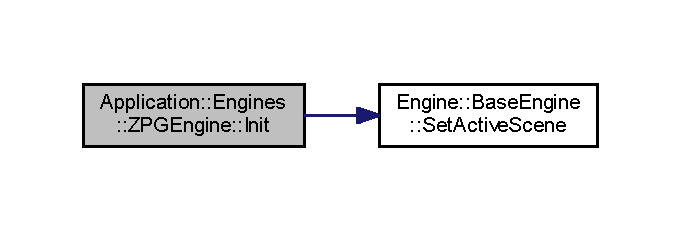
\includegraphics[width=327pt]{classApplication_1_1Engines_1_1ZPGEngine_a08a065a6200bf4465b71efa08f173cc5_cgraph}
\end{center}
\end{figure}
\mbox{\Hypertarget{classEngine_1_1BaseEngine_a7a1c9b833049b3eb61194cab113dfe89}\label{classEngine_1_1BaseEngine_a7a1c9b833049b3eb61194cab113dfe89}} 
\index{Application\+::\+Engines\+::\+Z\+P\+G\+Engine@{Application\+::\+Engines\+::\+Z\+P\+G\+Engine}!Init\+Success@{Init\+Success}}
\index{Init\+Success@{Init\+Success}!Application\+::\+Engines\+::\+Z\+P\+G\+Engine@{Application\+::\+Engines\+::\+Z\+P\+G\+Engine}}
\subsubsection{\texorpdfstring{Init\+Success()}{InitSuccess()}}
{\footnotesize\ttfamily bool Engine\+::\+Base\+Engine\+::\+Init\+Success (\begin{DoxyParamCaption}{ }\end{DoxyParamCaption})\hspace{0.3cm}{\ttfamily [inherited]}}



Definition at line 46 of file Base\+Engine.\+cpp.


\begin{DoxyCode}
47 \{
48     \textcolor{keywordflow}{return} \mbox{\hyperlink{classEngine_1_1BaseEngine_a79e265845b321c0e9822fb170c564e55}{\_init}};
49 \}
\end{DoxyCode}
\mbox{\Hypertarget{classEngine_1_1BaseEngine_afc82c6a00d5a9d4714740fc5eab5db86}\label{classEngine_1_1BaseEngine_afc82c6a00d5a9d4714740fc5eab5db86}} 
\index{Application\+::\+Engines\+::\+Z\+P\+G\+Engine@{Application\+::\+Engines\+::\+Z\+P\+G\+Engine}!Set\+Active\+Scene@{Set\+Active\+Scene}}
\index{Set\+Active\+Scene@{Set\+Active\+Scene}!Application\+::\+Engines\+::\+Z\+P\+G\+Engine@{Application\+::\+Engines\+::\+Z\+P\+G\+Engine}}
\subsubsection{\texorpdfstring{Set\+Active\+Scene()}{SetActiveScene()}}
{\footnotesize\ttfamily void Engine\+::\+Base\+Engine\+::\+Set\+Active\+Scene (\begin{DoxyParamCaption}\item[{\mbox{\hyperlink{classEngine_1_1Components_1_1Scene}{Components\+::\+Scene}} $\ast$}]{scene = {\ttfamily nullptr} }\end{DoxyParamCaption})\hspace{0.3cm}{\ttfamily [virtual]}, {\ttfamily [inherited]}}



Definition at line 132 of file Base\+Engine.\+cpp.



Referenced by Application\+::\+Engines\+::\+Basic\+Engine\+::\+Init(), Init(), Application\+::\+Engines\+::\+Triangle\+Engine\+::\+Init(), Application\+::\+Engines\+::\+Camera\+Engine\+::\+Init(), and Application\+::\+Engines\+::\+Light\+Engine\+::\+Init().


\begin{DoxyCode}
133 \{
134     \textcolor{keywordflow}{if} (scene == \textcolor{keyword}{nullptr} && !\mbox{\hyperlink{classEngine_1_1BaseEngine_afd02af3c2fbe9bb734db014dec06585a}{Scenes}}->empty())
135         \mbox{\hyperlink{classEngine_1_1BaseEngine_adb3dbc839da9d821e08b18d8a221698d}{ActiveScene}} = \mbox{\hyperlink{classEngine_1_1BaseEngine_afd02af3c2fbe9bb734db014dec06585a}{Scenes}}->begin()->second;
136     \textcolor{keywordflow}{else}
137         \mbox{\hyperlink{classEngine_1_1BaseEngine_adb3dbc839da9d821e08b18d8a221698d}{ActiveScene}} = scene;     
138 \}
\end{DoxyCode}
Here is the caller graph for this function\+:
\nopagebreak
\begin{figure}[H]
\begin{center}
\leavevmode
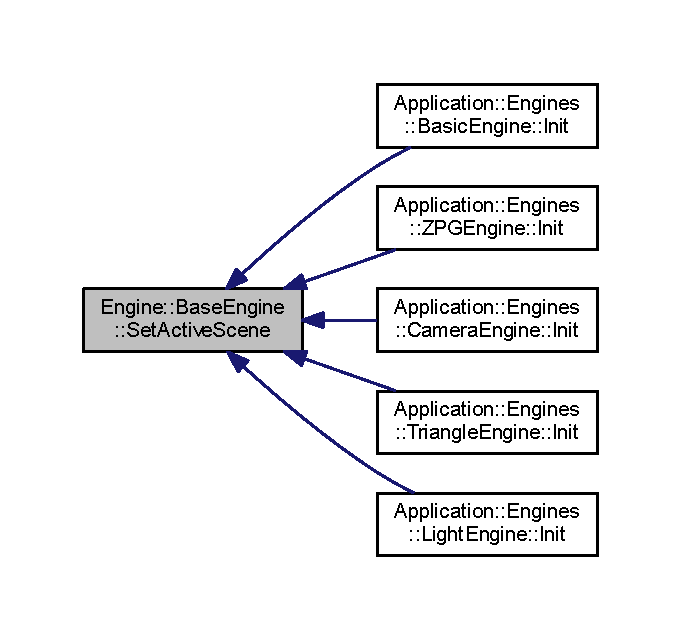
\includegraphics[width=327pt]{classEngine_1_1BaseEngine_afc82c6a00d5a9d4714740fc5eab5db86_icgraph}
\end{center}
\end{figure}
\mbox{\Hypertarget{classEngine_1_1BaseEngine_a525fdc7a1da7eecb514ad5763f06be79}\label{classEngine_1_1BaseEngine_a525fdc7a1da7eecb514ad5763f06be79}} 
\index{Application\+::\+Engines\+::\+Z\+P\+G\+Engine@{Application\+::\+Engines\+::\+Z\+P\+G\+Engine}!Start@{Start}}
\index{Start@{Start}!Application\+::\+Engines\+::\+Z\+P\+G\+Engine@{Application\+::\+Engines\+::\+Z\+P\+G\+Engine}}
\subsubsection{\texorpdfstring{Start()}{Start()}}
{\footnotesize\ttfamily void Engine\+::\+Base\+Engine\+::\+Start (\begin{DoxyParamCaption}{ }\end{DoxyParamCaption})\hspace{0.3cm}{\ttfamily [virtual]}, {\ttfamily [inherited]}}



Definition at line 126 of file Base\+Engine.\+cpp.



Referenced by main().


\begin{DoxyCode}
127 \{
128     system(\textcolor{stringliteral}{"cls"});
129     \mbox{\hyperlink{classEngine_1_1BaseEngine_aad3c237ca657b9f22f76fccf7fc7561f}{UpdateInternal}}();
130 \}
\end{DoxyCode}
Here is the caller graph for this function\+:
\nopagebreak
\begin{figure}[H]
\begin{center}
\leavevmode
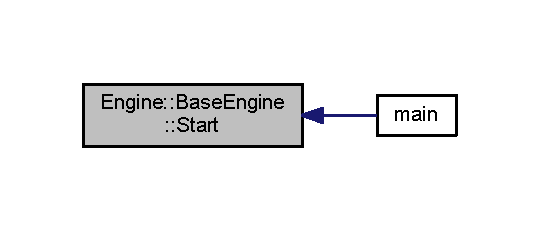
\includegraphics[width=259pt]{classEngine_1_1BaseEngine_a525fdc7a1da7eecb514ad5763f06be79_icgraph}
\end{center}
\end{figure}
\mbox{\Hypertarget{classApplication_1_1Engines_1_1ZPGEngine_a44b3d077ad688846aaa40d95ad14f851}\label{classApplication_1_1Engines_1_1ZPGEngine_a44b3d077ad688846aaa40d95ad14f851}} 
\index{Application\+::\+Engines\+::\+Z\+P\+G\+Engine@{Application\+::\+Engines\+::\+Z\+P\+G\+Engine}!Update@{Update}}
\index{Update@{Update}!Application\+::\+Engines\+::\+Z\+P\+G\+Engine@{Application\+::\+Engines\+::\+Z\+P\+G\+Engine}}
\subsubsection{\texorpdfstring{Update()}{Update()}\hspace{0.1cm}{\footnotesize\ttfamily [1/2]}}
{\footnotesize\ttfamily void Application\+::\+Engines\+::\+Z\+P\+G\+Engine\+::\+Update (\begin{DoxyParamCaption}\item[{\+::\mbox{\hyperlink{classEngine_1_1Components_1_1Window}{Engine\+::\+Components\+::\+Window}} $\ast$}]{window }\end{DoxyParamCaption})\hspace{0.3cm}{\ttfamily [override]}}



Definition at line 48 of file Z\+P\+G\+Engine.\+cpp.


\begin{DoxyCode}
49 \{
50     \textcolor{keywordflow}{for}(\textcolor{keyword}{auto} it = Objects->begin(); it != Objects->end(); ++it)
51     \{
52         \textcolor{comment}{/*ShaderProgram->Shaders[0]->SendUniform(ShaderProgram, "modelMatrix", M);}
53 \textcolor{comment}{        ShaderProgram->Shaders[1]->SendUniform(ShaderProgram, "color", \_angle-(long)\_angle);*/}
54         \textcolor{keyword}{auto} \textcolor{keywordtype}{object} = it->second;
55         \textcolor{comment}{//Handle Objects}
56         \textcolor{keywordtype}{object}->Program->Use();
57         \textcolor{keywordtype}{object}->Program->Shaders->Get(\textcolor{stringliteral}{"vertex"})->SendUniform(object->Program, \textcolor{stringliteral}{"modelMatrix"}, 
      \mbox{\hyperlink{classApplication_1_1Engines_1_1ZPGEngine_a6e982d6b97e8d538cdf8df9a7f4c6cd0}{M}});
58         \textcolor{keywordtype}{object}->Program->Shaders->Get(\textcolor{stringliteral}{"fragment"})->SendUniform(object->Program, \textcolor{stringliteral}{"color"}, 
      \mbox{\hyperlink{classApplication_1_1Engines_1_1ZPGEngine_adee8aa02ea2c15751eb6222bded1f729}{angle}} - (\textcolor{keywordtype}{long})\mbox{\hyperlink{classApplication_1_1Engines_1_1ZPGEngine_adee8aa02ea2c15751eb6222bded1f729}{angle}});
59         \textcolor{keywordtype}{object}->Draw();
60         \mbox{\hyperlink{classApplication_1_1Engines_1_1ZPGEngine_adee8aa02ea2c15751eb6222bded1f729}{angle}} += 0.1f;
61     \}
62 \}
\end{DoxyCode}
\mbox{\Hypertarget{classEngine_1_1BaseEngine_a01c23c2073f08939a660f3b7a866852c}\label{classEngine_1_1BaseEngine_a01c23c2073f08939a660f3b7a866852c}} 
\index{Application\+::\+Engines\+::\+Z\+P\+G\+Engine@{Application\+::\+Engines\+::\+Z\+P\+G\+Engine}!Update@{Update}}
\index{Update@{Update}!Application\+::\+Engines\+::\+Z\+P\+G\+Engine@{Application\+::\+Engines\+::\+Z\+P\+G\+Engine}}
\subsubsection{\texorpdfstring{Update()}{Update()}\hspace{0.1cm}{\footnotesize\ttfamily [2/2]}}
{\footnotesize\ttfamily void Engine\+::\+Base\+Engine\+::\+Update (\begin{DoxyParamCaption}\item[{\mbox{\hyperlink{classEngine_1_1Components_1_1Window}{Components\+::\+Window}} $\ast$}]{window }\end{DoxyParamCaption})\hspace{0.3cm}{\ttfamily [virtual]}, {\ttfamily [inherited]}}



Definition at line 112 of file Base\+Engine.\+cpp.


\begin{DoxyCode}
113 \{
114 \}
\end{DoxyCode}
\mbox{\Hypertarget{classEngine_1_1BaseEngine_aace6be2a42d12b64fbd35f1acdb08408}\label{classEngine_1_1BaseEngine_aace6be2a42d12b64fbd35f1acdb08408}} 
\index{Application\+::\+Engines\+::\+Z\+P\+G\+Engine@{Application\+::\+Engines\+::\+Z\+P\+G\+Engine}!Update\+Begin@{Update\+Begin}}
\index{Update\+Begin@{Update\+Begin}!Application\+::\+Engines\+::\+Z\+P\+G\+Engine@{Application\+::\+Engines\+::\+Z\+P\+G\+Engine}}
\subsubsection{\texorpdfstring{Update\+Begin()}{UpdateBegin()}}
{\footnotesize\ttfamily void Engine\+::\+Base\+Engine\+::\+Update\+Begin (\begin{DoxyParamCaption}\item[{\mbox{\hyperlink{classEngine_1_1Components_1_1Window}{Components\+::\+Window}} $\ast$}]{window }\end{DoxyParamCaption})\hspace{0.3cm}{\ttfamily [virtual]}, {\ttfamily [inherited]}}



Definition at line 57 of file Base\+Engine.\+cpp.



References Engine\+::\+Components\+::\+Window\+::\+Get().


\begin{DoxyCode}
58 \{
59     \textcolor{comment}{// Scene}
60     \mbox{\hyperlink{classEngine_1_1BaseEngine_adb3dbc839da9d821e08b18d8a221698d}{ActiveScene}}->\mbox{\hyperlink{classEngine_1_1Components_1_1Scene_af18bd334fe66952b8d79b8e9e99ab2d8}{BeginLoad}}(\textcolor{keyword}{this});
61 
62     \textcolor{comment}{// Buffers}
63     glEnable(GL\_DEPTH\_TEST);
64     glDepthFunc(GL\_LESS);
65     glClear(GL\_COLOR\_BUFFER\_BIT | GL\_DEPTH\_BUFFER\_BIT);
66 
67     \textcolor{comment}{// Input}
68     \textcolor{keywordtype}{short} mouseKeysActive = 0;
69     glfwGetCursorPos(window->Get(), &\mbox{\hyperlink{classEngine_1_1BaseEngine_a5fe085152ebe93346900407f6b41a034}{MouseX}}, &\mbox{\hyperlink{classEngine_1_1BaseEngine_a143c9c32dbbdc70bf1546ffe275bf384}{MouseY}});
70     \textcolor{keywordflow}{for}(\textcolor{keywordtype}{short} i = 0; i < 8; i++)
71     \{
72         \textcolor{keyword}{const} \textcolor{keywordtype}{int} state = glfwGetMouseButton(window->Get(), i);
73         \textcolor{keyword}{auto} value = \mbox{\hyperlink{classEngine_1_1BaseEngine_a3ee2bdddb66d45b8c808ffd937ba9c50}{MouseKeys}}[i];
74         \textcolor{comment}{// flip state}
75         \textcolor{keywordflow}{if} (state == GLFW\_PRESS && !value)
76             \mbox{\hyperlink{classEngine_1_1BaseEngine_a3ee2bdddb66d45b8c808ffd937ba9c50}{MouseKeys}}.\mbox{\hyperlink{classGeneric_1_1Dictionary_ae7cb006f801b21c172e8fbac8794fa99}{Add}}(i, \textcolor{keyword}{true});
77         \textcolor{keywordflow}{else} \textcolor{keywordflow}{if} (state == GLFW\_RELEASE && value)
78             \mbox{\hyperlink{classEngine_1_1BaseEngine_a3ee2bdddb66d45b8c808ffd937ba9c50}{MouseKeys}}.\mbox{\hyperlink{classGeneric_1_1Dictionary_ae7cb006f801b21c172e8fbac8794fa99}{Add}}(i, \textcolor{keyword}{false});
79         \textcolor{keywordflow}{if} (\mbox{\hyperlink{classEngine_1_1BaseEngine_a3ee2bdddb66d45b8c808ffd937ba9c50}{MouseKeys}}[i])
80             mouseKeysActive++;
81     \}
82     \textcolor{keywordtype}{short} keysActive = 0;
83     SetConsoleCursorPosition(GetStdHandle(STD\_OUTPUT\_HANDLE), \{ 40, keysActive \});
84     fprintf(\mbox{\hyperlink{classEngine_1_1BaseEngine_a26fd54a1ee2733f9c654af5afcfa96cf}{\_errorStream}}, \textcolor{stringliteral}{"                           "});
85     \textcolor{keywordflow}{for} (\textcolor{keywordtype}{short} i = 1; i < 512; i++)
86     \{
87         \textcolor{keyword}{const} \textcolor{keywordtype}{int} state = glfwGetKey(window->Get(), i);
88         \textcolor{keyword}{auto} value = \mbox{\hyperlink{classEngine_1_1BaseEngine_a65321a97e83f0a6ee90df3efac2d3307}{Keys}}[i];
89         \textcolor{comment}{// flip state}
90         \textcolor{keywordflow}{if} (state == GLFW\_PRESS && !value)
91             \mbox{\hyperlink{classEngine_1_1BaseEngine_a65321a97e83f0a6ee90df3efac2d3307}{Keys}}.\mbox{\hyperlink{classGeneric_1_1Dictionary_ae7cb006f801b21c172e8fbac8794fa99}{Add}}(i, \textcolor{keyword}{true});
92         \textcolor{keywordflow}{else} \textcolor{keywordflow}{if} (state == GLFW\_RELEASE && value)
93             \mbox{\hyperlink{classEngine_1_1BaseEngine_a65321a97e83f0a6ee90df3efac2d3307}{Keys}}.\mbox{\hyperlink{classGeneric_1_1Dictionary_ae7cb006f801b21c172e8fbac8794fa99}{Add}}(i, \textcolor{keyword}{false});
94         \textcolor{keywordflow}{if} (\mbox{\hyperlink{classEngine_1_1BaseEngine_a65321a97e83f0a6ee90df3efac2d3307}{Keys}}[i])
95             keysActive++;
96     \}
97     \textcolor{keywordtype}{bool} handleKeys = \textcolor{keyword}{true},
98          handleMouse = \textcolor{keyword}{true};
99     \textcolor{keywordflow}{for} (\textcolor{keyword}{auto} handler : *\mbox{\hyperlink{classEngine_1_1BaseEngine_a134fa082c5a64d62b76ddf926647e7cc}{InputHandlers}})
100     \{
101         \textcolor{keywordflow}{if}(handleKeys)
102             handleKeys = handler->HandleKeys(\textcolor{keyword}{this}, window, \mbox{\hyperlink{classEngine_1_1BaseEngine_adb3dbc839da9d821e08b18d8a221698d}{ActiveScene}}, 
      \mbox{\hyperlink{classEngine_1_1BaseEngine_a65321a97e83f0a6ee90df3efac2d3307}{Keys}}, keysActive);
103         \textcolor{keywordflow}{if}(handleMouse)
104             handleMouse = handler->HandleMouse(\textcolor{keyword}{this}, window, \mbox{\hyperlink{classEngine_1_1BaseEngine_adb3dbc839da9d821e08b18d8a221698d}{ActiveScene}}, 
      \mbox{\hyperlink{classEngine_1_1BaseEngine_a5fe085152ebe93346900407f6b41a034}{MouseX}}, \mbox{\hyperlink{classEngine_1_1BaseEngine_a143c9c32dbbdc70bf1546ffe275bf384}{MouseY}}, \mbox{\hyperlink{classEngine_1_1BaseEngine_a3ee2bdddb66d45b8c808ffd937ba9c50}{MouseKeys}}, mouseKeysActive);
105         \textcolor{keywordflow}{if}(!handleKeys && !handleMouse)
106             \textcolor{keywordflow}{break};
107     \}
108 
109     SetConsoleCursorPosition(GetStdHandle(STD\_OUTPUT\_HANDLE), \{ 0,0 \});
110 \}
\end{DoxyCode}
Here is the call graph for this function\+:
\nopagebreak
\begin{figure}[H]
\begin{center}
\leavevmode
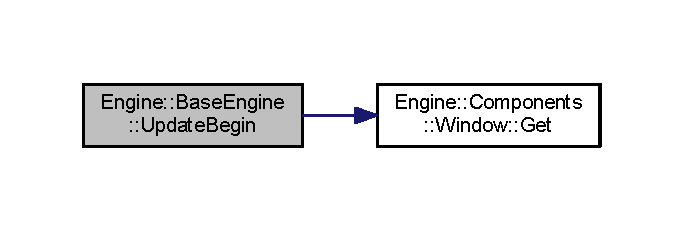
\includegraphics[width=328pt]{classEngine_1_1BaseEngine_aace6be2a42d12b64fbd35f1acdb08408_cgraph}
\end{center}
\end{figure}
\mbox{\Hypertarget{classEngine_1_1BaseEngine_a7c07c98e583df042a0eb01e0ddec85a1}\label{classEngine_1_1BaseEngine_a7c07c98e583df042a0eb01e0ddec85a1}} 
\index{Application\+::\+Engines\+::\+Z\+P\+G\+Engine@{Application\+::\+Engines\+::\+Z\+P\+G\+Engine}!Update\+End@{Update\+End}}
\index{Update\+End@{Update\+End}!Application\+::\+Engines\+::\+Z\+P\+G\+Engine@{Application\+::\+Engines\+::\+Z\+P\+G\+Engine}}
\subsubsection{\texorpdfstring{Update\+End()}{UpdateEnd()}}
{\footnotesize\ttfamily void Engine\+::\+Base\+Engine\+::\+Update\+End (\begin{DoxyParamCaption}\item[{\mbox{\hyperlink{classEngine_1_1Components_1_1Window}{Components\+::\+Window}} $\ast$}]{window }\end{DoxyParamCaption})\hspace{0.3cm}{\ttfamily [virtual]}, {\ttfamily [inherited]}}



Definition at line 116 of file Base\+Engine.\+cpp.



References Engine\+::\+Components\+::\+Window\+::\+Get().


\begin{DoxyCode}
117 \{
118     \textcolor{comment}{// update other events like input handling}
119     glfwPollEvents();
120     \textcolor{comment}{// put the stuff we’ve been drawing onto the display}
121     glfwSwapBuffers(window->Get());
122 
123     \mbox{\hyperlink{classEngine_1_1BaseEngine_adb3dbc839da9d821e08b18d8a221698d}{ActiveScene}}->\mbox{\hyperlink{classEngine_1_1Components_1_1Scene_abd8fcdcac52dbce6a0a18de3860ab087}{FrameUpdate}}(\textcolor{keyword}{this});
124 \}
\end{DoxyCode}
Here is the call graph for this function\+:
\nopagebreak
\begin{figure}[H]
\begin{center}
\leavevmode
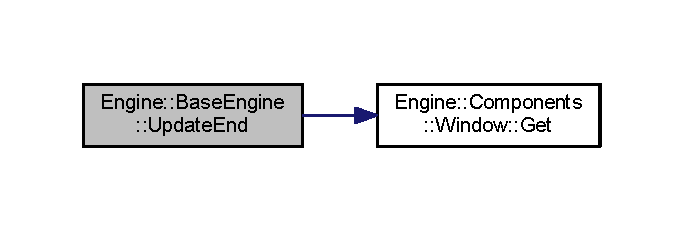
\includegraphics[width=328pt]{classEngine_1_1BaseEngine_a7c07c98e583df042a0eb01e0ddec85a1_cgraph}
\end{center}
\end{figure}


\subsection{Member Data Documentation}
\mbox{\Hypertarget{classEngine_1_1BaseEngine_adb3dbc839da9d821e08b18d8a221698d}\label{classEngine_1_1BaseEngine_adb3dbc839da9d821e08b18d8a221698d}} 
\index{Application\+::\+Engines\+::\+Z\+P\+G\+Engine@{Application\+::\+Engines\+::\+Z\+P\+G\+Engine}!Active\+Scene@{Active\+Scene}}
\index{Active\+Scene@{Active\+Scene}!Application\+::\+Engines\+::\+Z\+P\+G\+Engine@{Application\+::\+Engines\+::\+Z\+P\+G\+Engine}}
\subsubsection{\texorpdfstring{Active\+Scene}{ActiveScene}}
{\footnotesize\ttfamily Components\+::\+Scene$\ast$ Engine\+::\+Base\+Engine\+::\+Active\+Scene\hspace{0.3cm}{\ttfamily [inherited]}}



Definition at line 34 of file Base\+Engine.\+h.



Referenced by Engine\+::\+Base\+Engine\+::\+Base\+Engine(), Application\+::\+Engines\+::\+Camera\+Engine\+::\+Init(), and Application\+::\+Engines\+::\+Light\+Engine\+::\+Init().

\mbox{\Hypertarget{classApplication_1_1Engines_1_1ZPGEngine_adee8aa02ea2c15751eb6222bded1f729}\label{classApplication_1_1Engines_1_1ZPGEngine_adee8aa02ea2c15751eb6222bded1f729}} 
\index{Application\+::\+Engines\+::\+Z\+P\+G\+Engine@{Application\+::\+Engines\+::\+Z\+P\+G\+Engine}!angle@{angle}}
\index{angle@{angle}!Application\+::\+Engines\+::\+Z\+P\+G\+Engine@{Application\+::\+Engines\+::\+Z\+P\+G\+Engine}}
\subsubsection{\texorpdfstring{angle}{angle}}
{\footnotesize\ttfamily float Application\+::\+Engines\+::\+Z\+P\+G\+Engine\+::angle\hspace{0.3cm}{\ttfamily [private]}}



Definition at line 15 of file Z\+P\+G\+Engine.\+h.



Referenced by Init().

\mbox{\Hypertarget{classEngine_1_1BaseEngine_a134fa082c5a64d62b76ddf926647e7cc}\label{classEngine_1_1BaseEngine_a134fa082c5a64d62b76ddf926647e7cc}} 
\index{Application\+::\+Engines\+::\+Z\+P\+G\+Engine@{Application\+::\+Engines\+::\+Z\+P\+G\+Engine}!Input\+Handlers@{Input\+Handlers}}
\index{Input\+Handlers@{Input\+Handlers}!Application\+::\+Engines\+::\+Z\+P\+G\+Engine@{Application\+::\+Engines\+::\+Z\+P\+G\+Engine}}
\subsubsection{\texorpdfstring{Input\+Handlers}{InputHandlers}}
{\footnotesize\ttfamily \mbox{\hyperlink{classGeneric_1_1Collection}{Generic\+::\+Collection}}$<$Components\+::\+I\+Input\+Handler$\ast$$>$$\ast$ Engine\+::\+Base\+Engine\+::\+Input\+Handlers\hspace{0.3cm}{\ttfamily [inherited]}}



Definition at line 31 of file Base\+Engine.\+h.



Referenced by Engine\+::\+Base\+Engine\+::\+Base\+Engine(), and Application\+::\+Engines\+::\+Light\+Engine\+::\+Init().

\mbox{\Hypertarget{classEngine_1_1BaseEngine_a65321a97e83f0a6ee90df3efac2d3307}\label{classEngine_1_1BaseEngine_a65321a97e83f0a6ee90df3efac2d3307}} 
\index{Application\+::\+Engines\+::\+Z\+P\+G\+Engine@{Application\+::\+Engines\+::\+Z\+P\+G\+Engine}!Keys@{Keys}}
\index{Keys@{Keys}!Application\+::\+Engines\+::\+Z\+P\+G\+Engine@{Application\+::\+Engines\+::\+Z\+P\+G\+Engine}}
\subsubsection{\texorpdfstring{Keys}{Keys}}
{\footnotesize\ttfamily \mbox{\hyperlink{classGeneric_1_1Dictionary}{Generic\+::\+Dictionary}}$<$short, bool$>$ Engine\+::\+Base\+Engine\+::\+Keys\hspace{0.3cm}{\ttfamily [inherited]}}



Definition at line 32 of file Base\+Engine.\+h.



Referenced by Engine\+::\+Base\+Engine\+::\+Base\+Engine().

\mbox{\Hypertarget{classApplication_1_1Engines_1_1ZPGEngine_a6e982d6b97e8d538cdf8df9a7f4c6cd0}\label{classApplication_1_1Engines_1_1ZPGEngine_a6e982d6b97e8d538cdf8df9a7f4c6cd0}} 
\index{Application\+::\+Engines\+::\+Z\+P\+G\+Engine@{Application\+::\+Engines\+::\+Z\+P\+G\+Engine}!M@{M}}
\index{M@{M}!Application\+::\+Engines\+::\+Z\+P\+G\+Engine@{Application\+::\+Engines\+::\+Z\+P\+G\+Engine}}
\subsubsection{\texorpdfstring{M}{M}}
{\footnotesize\ttfamily glm\+::mat4 Application\+::\+Engines\+::\+Z\+P\+G\+Engine\+::M\hspace{0.3cm}{\ttfamily [private]}}



Definition at line 14 of file Z\+P\+G\+Engine.\+h.



Referenced by Init().

\mbox{\Hypertarget{classEngine_1_1BaseEngine_a3ee2bdddb66d45b8c808ffd937ba9c50}\label{classEngine_1_1BaseEngine_a3ee2bdddb66d45b8c808ffd937ba9c50}} 
\index{Application\+::\+Engines\+::\+Z\+P\+G\+Engine@{Application\+::\+Engines\+::\+Z\+P\+G\+Engine}!Mouse\+Keys@{Mouse\+Keys}}
\index{Mouse\+Keys@{Mouse\+Keys}!Application\+::\+Engines\+::\+Z\+P\+G\+Engine@{Application\+::\+Engines\+::\+Z\+P\+G\+Engine}}
\subsubsection{\texorpdfstring{Mouse\+Keys}{MouseKeys}}
{\footnotesize\ttfamily \mbox{\hyperlink{classGeneric_1_1Dictionary}{Generic\+::\+Dictionary}}$<$short, bool$>$ Engine\+::\+Base\+Engine\+::\+Mouse\+Keys\hspace{0.3cm}{\ttfamily [inherited]}}



Definition at line 33 of file Base\+Engine.\+h.



Referenced by Engine\+::\+Base\+Engine\+::\+Base\+Engine().

\mbox{\Hypertarget{classEngine_1_1BaseEngine_a5fe085152ebe93346900407f6b41a034}\label{classEngine_1_1BaseEngine_a5fe085152ebe93346900407f6b41a034}} 
\index{Application\+::\+Engines\+::\+Z\+P\+G\+Engine@{Application\+::\+Engines\+::\+Z\+P\+G\+Engine}!MouseX@{MouseX}}
\index{MouseX@{MouseX}!Application\+::\+Engines\+::\+Z\+P\+G\+Engine@{Application\+::\+Engines\+::\+Z\+P\+G\+Engine}}
\subsubsection{\texorpdfstring{MouseX}{MouseX}}
{\footnotesize\ttfamily double Engine\+::\+Base\+Engine\+::\+MouseX\hspace{0.3cm}{\ttfamily [inherited]}}



Definition at line 35 of file Base\+Engine.\+h.

\mbox{\Hypertarget{classEngine_1_1BaseEngine_a143c9c32dbbdc70bf1546ffe275bf384}\label{classEngine_1_1BaseEngine_a143c9c32dbbdc70bf1546ffe275bf384}} 
\index{Application\+::\+Engines\+::\+Z\+P\+G\+Engine@{Application\+::\+Engines\+::\+Z\+P\+G\+Engine}!MouseY@{MouseY}}
\index{MouseY@{MouseY}!Application\+::\+Engines\+::\+Z\+P\+G\+Engine@{Application\+::\+Engines\+::\+Z\+P\+G\+Engine}}
\subsubsection{\texorpdfstring{MouseY}{MouseY}}
{\footnotesize\ttfamily double Engine\+::\+Base\+Engine\+::\+MouseY\hspace{0.3cm}{\ttfamily [inherited]}}



Definition at line 36 of file Base\+Engine.\+h.

\mbox{\Hypertarget{classEngine_1_1BaseEngine_ae0f86360ea3a384caefe443dd8f88601}\label{classEngine_1_1BaseEngine_ae0f86360ea3a384caefe443dd8f88601}} 
\index{Application\+::\+Engines\+::\+Z\+P\+G\+Engine@{Application\+::\+Engines\+::\+Z\+P\+G\+Engine}!Programs@{Programs}}
\index{Programs@{Programs}!Application\+::\+Engines\+::\+Z\+P\+G\+Engine@{Application\+::\+Engines\+::\+Z\+P\+G\+Engine}}
\subsubsection{\texorpdfstring{Programs}{Programs}}
{\footnotesize\ttfamily \mbox{\hyperlink{classGeneric_1_1Dictionary}{Generic\+::\+Dictionary}}$<$std\+::string, Components\+::\+Graphics\+::\+Program$\ast$$>$$\ast$ Engine\+::\+Base\+Engine\+::\+Programs\hspace{0.3cm}{\ttfamily [inherited]}}



Definition at line 28 of file Base\+Engine.\+h.



Referenced by Engine\+::\+Base\+Engine\+::\+Base\+Engine(), Application\+::\+Input\+::\+Handlers\+::\+Camera\+Input\+Handler\+::\+Handle\+Mouse(), Init(), Application\+::\+Engines\+::\+Triangle\+Engine\+::\+Init(), Application\+::\+Engines\+::\+Basic\+Engine\+::\+Init(), Application\+::\+Engines\+::\+Camera\+Engine\+::\+Init(), Application\+::\+Engines\+::\+Light\+Engine\+::\+Init(), Application\+::\+Scenes\+::\+Triangle\+Scene\+::\+Load(), and Application\+::\+Scenes\+::\+Sphere\+Scene\+::\+Load().

\mbox{\Hypertarget{classEngine_1_1BaseEngine_afd02af3c2fbe9bb734db014dec06585a}\label{classEngine_1_1BaseEngine_afd02af3c2fbe9bb734db014dec06585a}} 
\index{Application\+::\+Engines\+::\+Z\+P\+G\+Engine@{Application\+::\+Engines\+::\+Z\+P\+G\+Engine}!Scenes@{Scenes}}
\index{Scenes@{Scenes}!Application\+::\+Engines\+::\+Z\+P\+G\+Engine@{Application\+::\+Engines\+::\+Z\+P\+G\+Engine}}
\subsubsection{\texorpdfstring{Scenes}{Scenes}}
{\footnotesize\ttfamily \mbox{\hyperlink{classGeneric_1_1Dictionary}{Generic\+::\+Dictionary}}$<$std\+::string, Components\+::\+Scene$\ast$$>$$\ast$ Engine\+::\+Base\+Engine\+::\+Scenes\hspace{0.3cm}{\ttfamily [inherited]}}



Definition at line 30 of file Base\+Engine.\+h.



Referenced by Engine\+::\+Base\+Engine\+::\+Base\+Engine(), Init(), Application\+::\+Engines\+::\+Triangle\+Engine\+::\+Init(), Application\+::\+Engines\+::\+Basic\+Engine\+::\+Init(), Application\+::\+Engines\+::\+Camera\+Engine\+::\+Init(), and Application\+::\+Engines\+::\+Light\+Engine\+::\+Init().

\mbox{\Hypertarget{classEngine_1_1BaseEngine_a2582dee3f73da82bb422b43317b85e3b}\label{classEngine_1_1BaseEngine_a2582dee3f73da82bb422b43317b85e3b}} 
\index{Application\+::\+Engines\+::\+Z\+P\+G\+Engine@{Application\+::\+Engines\+::\+Z\+P\+G\+Engine}!Shaders@{Shaders}}
\index{Shaders@{Shaders}!Application\+::\+Engines\+::\+Z\+P\+G\+Engine@{Application\+::\+Engines\+::\+Z\+P\+G\+Engine}}
\subsubsection{\texorpdfstring{Shaders}{Shaders}}
{\footnotesize\ttfamily \mbox{\hyperlink{classGeneric_1_1Dictionary}{Generic\+::\+Dictionary}}$<$std\+::string, Components\+::\+Graphics\+::\+Shader$\ast$$>$$\ast$ Engine\+::\+Base\+Engine\+::\+Shaders\hspace{0.3cm}{\ttfamily [inherited]}}



Definition at line 29 of file Base\+Engine.\+h.



Referenced by Engine\+::\+Base\+Engine\+::\+Base\+Engine(), Application\+::\+Input\+::\+Handlers\+::\+Camera\+Input\+Handler\+::\+Handle\+Mouse(), Application\+::\+Engines\+::\+Triangle\+Engine\+::\+Init(), Init(), Application\+::\+Engines\+::\+Basic\+Engine\+::\+Init(), Application\+::\+Engines\+::\+Camera\+Engine\+::\+Init(), and Application\+::\+Engines\+::\+Light\+Engine\+::\+Init().

\mbox{\Hypertarget{classEngine_1_1BaseEngine_a4a1a4c4dae052e66ecc4f326eeed4d33}\label{classEngine_1_1BaseEngine_a4a1a4c4dae052e66ecc4f326eeed4d33}} 
\index{Application\+::\+Engines\+::\+Z\+P\+G\+Engine@{Application\+::\+Engines\+::\+Z\+P\+G\+Engine}!Windows@{Windows}}
\index{Windows@{Windows}!Application\+::\+Engines\+::\+Z\+P\+G\+Engine@{Application\+::\+Engines\+::\+Z\+P\+G\+Engine}}
\subsubsection{\texorpdfstring{Windows}{Windows}}
{\footnotesize\ttfamily \mbox{\hyperlink{classGeneric_1_1Dictionary}{Generic\+::\+Dictionary}}$<$std\+::string, Components\+::\+Window$\ast$$>$$\ast$ Engine\+::\+Base\+Engine\+::\+Windows\hspace{0.3cm}{\ttfamily [inherited]}}



Definition at line 27 of file Base\+Engine.\+h.



Referenced by Engine\+::\+Base\+Engine\+::\+Base\+Engine(), Init(), Application\+::\+Engines\+::\+Triangle\+Engine\+::\+Init(), Application\+::\+Engines\+::\+Basic\+Engine\+::\+Init(), Application\+::\+Engines\+::\+Camera\+Engine\+::\+Init(), and Application\+::\+Engines\+::\+Light\+Engine\+::\+Init().



The documentation for this class was generated from the following files\+:\begin{DoxyCompactItemize}
\item 
Z\+P\+G/\mbox{\hyperlink{ZPGEngine_8h}{Z\+P\+G\+Engine.\+h}}\item 
Z\+P\+G/\mbox{\hyperlink{ZPGEngine_8cpp}{Z\+P\+G\+Engine.\+cpp}}\end{DoxyCompactItemize}

\hypertarget{classApplication_1_1Input_1_1Handlers_1_1CameraInputHandler}{}\section{Application\+:\+:Input\+:\+:Handlers\+:\+:Camera\+Input\+Handler Class Reference}
\label{classApplication_1_1Input_1_1Handlers_1_1CameraInputHandler}\index{Application\+::\+Input\+::\+Handlers\+::\+Camera\+Input\+Handler@{Application\+::\+Input\+::\+Handlers\+::\+Camera\+Input\+Handler}}


{\ttfamily \#include $<$Camera\+Input\+Handler.\+h$>$}



Inheritance diagram for Application\+:\+:Input\+:\+:Handlers\+:\+:Camera\+Input\+Handler\+:
\nopagebreak
\begin{figure}[H]
\begin{center}
\leavevmode
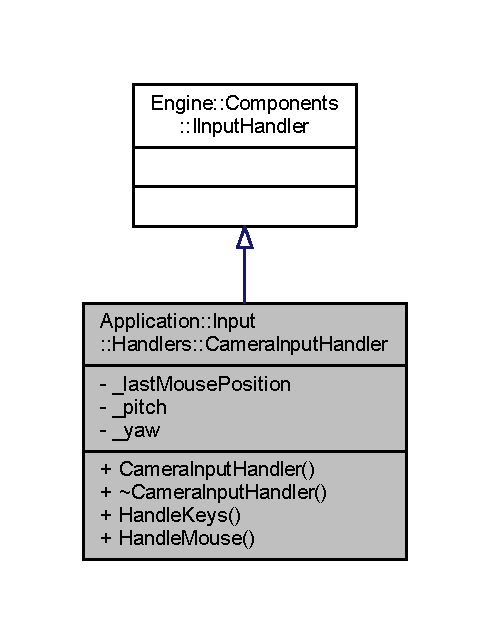
\includegraphics[width=235pt]{classApplication_1_1Input_1_1Handlers_1_1CameraInputHandler__inherit__graph}
\end{center}
\end{figure}


Collaboration diagram for Application\+:\+:Input\+:\+:Handlers\+:\+:Camera\+Input\+Handler\+:
\nopagebreak
\begin{figure}[H]
\begin{center}
\leavevmode
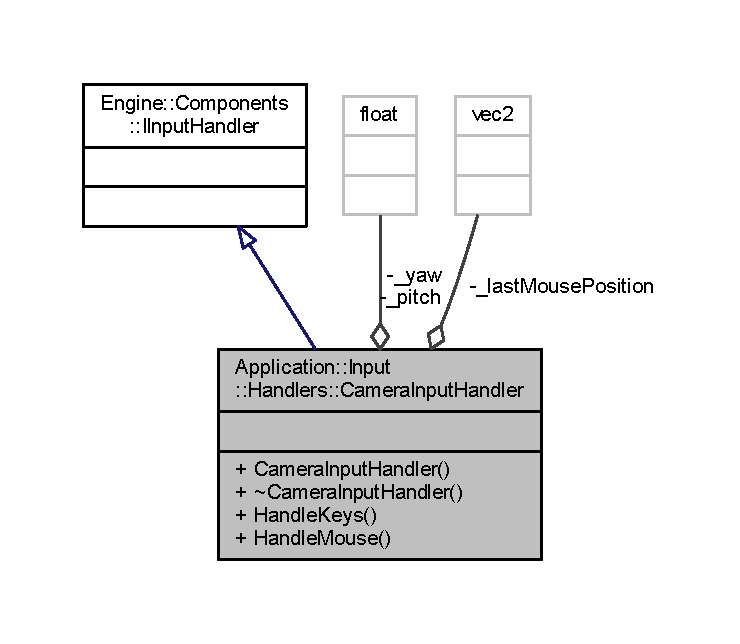
\includegraphics[width=350pt]{classApplication_1_1Input_1_1Handlers_1_1CameraInputHandler__coll__graph}
\end{center}
\end{figure}
\subsection*{Public Member Functions}
\begin{DoxyCompactItemize}
\item 
\mbox{\hyperlink{classApplication_1_1Input_1_1Handlers_1_1CameraInputHandler_a1863bafdf1002ddebe45795112c4c324}{Camera\+Input\+Handler}} ()
\item 
\mbox{\hyperlink{classApplication_1_1Input_1_1Handlers_1_1CameraInputHandler_a08ccb4be5e9da5e461b3b1905a8da90d}{$\sim$\+Camera\+Input\+Handler}} ()
\item 
bool \mbox{\hyperlink{classApplication_1_1Input_1_1Handlers_1_1CameraInputHandler_a149884ea2dc9deea39d3dcd10dfa74b1}{Handle\+Keys}} (\mbox{\hyperlink{classEngine_1_1BaseEngine}{Engine\+::\+Base\+Engine}} $\ast$engine, \mbox{\hyperlink{classEngine_1_1Components_1_1Window}{Engine\+::\+Components\+::\+Window}} $\ast$window, \mbox{\hyperlink{classEngine_1_1Components_1_1Scene}{Engine\+::\+Components\+::\+Scene}} $\ast$scene, \mbox{\hyperlink{classGeneric_1_1Dictionary}{Generic\+::\+Dictionary}}$<$ short, bool $>$ \&keys, int keys\+Active) override
\item 
bool \mbox{\hyperlink{classApplication_1_1Input_1_1Handlers_1_1CameraInputHandler_ab06fa94ce5265dc06abb645ea29850bd}{Handle\+Mouse}} (\mbox{\hyperlink{classEngine_1_1BaseEngine}{Engine\+::\+Base\+Engine}} $\ast$engine, \mbox{\hyperlink{classEngine_1_1Components_1_1Window}{Engine\+::\+Components\+::\+Window}} $\ast$window, \mbox{\hyperlink{classEngine_1_1Components_1_1Scene}{Engine\+::\+Components\+::\+Scene}} $\ast$scene, double x, double y, \mbox{\hyperlink{classGeneric_1_1Dictionary}{Generic\+::\+Dictionary}}$<$ short, bool $>$ \&keys, int keys\+Active) override
\end{DoxyCompactItemize}
\subsection*{Private Attributes}
\begin{DoxyCompactItemize}
\item 
glm\+::vec2 \mbox{\hyperlink{classApplication_1_1Input_1_1Handlers_1_1CameraInputHandler_ae8e329dd433afb42e5f53b5937a927fb}{\+\_\+last\+Mouse\+Position}}
\item 
float \mbox{\hyperlink{classApplication_1_1Input_1_1Handlers_1_1CameraInputHandler_a0157ef737743b53e5db833012cd27372}{\+\_\+pitch}}
\item 
float \mbox{\hyperlink{classApplication_1_1Input_1_1Handlers_1_1CameraInputHandler_a2fa09dcae6ed67d452d374a9fb629349}{\+\_\+yaw}}
\end{DoxyCompactItemize}


\subsection{Detailed Description}


Definition at line 11 of file Camera\+Input\+Handler.\+h.



\subsection{Constructor \& Destructor Documentation}
\mbox{\Hypertarget{classApplication_1_1Input_1_1Handlers_1_1CameraInputHandler_a1863bafdf1002ddebe45795112c4c324}\label{classApplication_1_1Input_1_1Handlers_1_1CameraInputHandler_a1863bafdf1002ddebe45795112c4c324}} 
\index{Application\+::\+Input\+::\+Handlers\+::\+Camera\+Input\+Handler@{Application\+::\+Input\+::\+Handlers\+::\+Camera\+Input\+Handler}!Camera\+Input\+Handler@{Camera\+Input\+Handler}}
\index{Camera\+Input\+Handler@{Camera\+Input\+Handler}!Application\+::\+Input\+::\+Handlers\+::\+Camera\+Input\+Handler@{Application\+::\+Input\+::\+Handlers\+::\+Camera\+Input\+Handler}}
\subsubsection{\texorpdfstring{Camera\+Input\+Handler()}{CameraInputHandler()}}
{\footnotesize\ttfamily Application\+::\+Input\+::\+Handlers\+::\+Camera\+Input\+Handler\+::\+Camera\+Input\+Handler (\begin{DoxyParamCaption}{ }\end{DoxyParamCaption})}



Definition at line 15 of file Camera\+Input\+Handler.\+cpp.



References \+\_\+last\+Mouse\+Position, \+\_\+pitch, and \+\_\+yaw.


\begin{DoxyCode}
16 \{
17     \mbox{\hyperlink{classApplication_1_1Input_1_1Handlers_1_1CameraInputHandler_ae8e329dd433afb42e5f53b5937a927fb}{\_lastMousePosition}} = glm::vec2(-1, -1);
18     \mbox{\hyperlink{classApplication_1_1Input_1_1Handlers_1_1CameraInputHandler_a2fa09dcae6ed67d452d374a9fb629349}{\_yaw}} = 0.f;
19     \mbox{\hyperlink{classApplication_1_1Input_1_1Handlers_1_1CameraInputHandler_a0157ef737743b53e5db833012cd27372}{\_pitch}} = 0.f;
20 \}
\end{DoxyCode}
\mbox{\Hypertarget{classApplication_1_1Input_1_1Handlers_1_1CameraInputHandler_a08ccb4be5e9da5e461b3b1905a8da90d}\label{classApplication_1_1Input_1_1Handlers_1_1CameraInputHandler_a08ccb4be5e9da5e461b3b1905a8da90d}} 
\index{Application\+::\+Input\+::\+Handlers\+::\+Camera\+Input\+Handler@{Application\+::\+Input\+::\+Handlers\+::\+Camera\+Input\+Handler}!````~Camera\+Input\+Handler@{$\sim$\+Camera\+Input\+Handler}}
\index{````~Camera\+Input\+Handler@{$\sim$\+Camera\+Input\+Handler}!Application\+::\+Input\+::\+Handlers\+::\+Camera\+Input\+Handler@{Application\+::\+Input\+::\+Handlers\+::\+Camera\+Input\+Handler}}
\subsubsection{\texorpdfstring{$\sim$\+Camera\+Input\+Handler()}{~CameraInputHandler()}}
{\footnotesize\ttfamily Application\+::\+Input\+::\+Handlers\+::\+Camera\+Input\+Handler\+::$\sim$\+Camera\+Input\+Handler (\begin{DoxyParamCaption}{ }\end{DoxyParamCaption})\hspace{0.3cm}{\ttfamily [default]}}



\subsection{Member Function Documentation}
\mbox{\Hypertarget{classApplication_1_1Input_1_1Handlers_1_1CameraInputHandler_a149884ea2dc9deea39d3dcd10dfa74b1}\label{classApplication_1_1Input_1_1Handlers_1_1CameraInputHandler_a149884ea2dc9deea39d3dcd10dfa74b1}} 
\index{Application\+::\+Input\+::\+Handlers\+::\+Camera\+Input\+Handler@{Application\+::\+Input\+::\+Handlers\+::\+Camera\+Input\+Handler}!Handle\+Keys@{Handle\+Keys}}
\index{Handle\+Keys@{Handle\+Keys}!Application\+::\+Input\+::\+Handlers\+::\+Camera\+Input\+Handler@{Application\+::\+Input\+::\+Handlers\+::\+Camera\+Input\+Handler}}
\subsubsection{\texorpdfstring{Handle\+Keys()}{HandleKeys()}}
{\footnotesize\ttfamily bool Application\+::\+Input\+::\+Handlers\+::\+Camera\+Input\+Handler\+::\+Handle\+Keys (\begin{DoxyParamCaption}\item[{\mbox{\hyperlink{classEngine_1_1BaseEngine}{Engine\+::\+Base\+Engine}} $\ast$}]{engine,  }\item[{\mbox{\hyperlink{classEngine_1_1Components_1_1Window}{Engine\+::\+Components\+::\+Window}} $\ast$}]{window,  }\item[{\mbox{\hyperlink{classEngine_1_1Components_1_1Scene}{Engine\+::\+Components\+::\+Scene}} $\ast$}]{scene,  }\item[{\mbox{\hyperlink{classGeneric_1_1Dictionary}{Generic\+::\+Dictionary}}$<$ short, bool $>$ \&}]{keys,  }\item[{int}]{keys\+Active }\end{DoxyParamCaption})\hspace{0.3cm}{\ttfamily [override]}}



Definition at line 25 of file Camera\+Input\+Handler.\+cpp.



References Engine\+::\+Components\+::\+Scene\+::\+Active\+Camera, Engine\+::\+Components\+::\+Camera\+::\+Direction, Engine\+::\+Components\+::\+Camera\+::\+Front, Engine\+::\+Components\+::\+Camera\+::\+Position, Engine\+::\+Components\+::\+Camera\+::\+Right, Engine\+::\+Components\+::\+Camera\+::\+Up, and Engine\+::\+Components\+::\+Camera\+::\+Update().


\begin{DoxyCode}
26 \{
27     \textcolor{keyword}{const} \textcolor{keywordtype}{float} speed = 0.2f;
28     glm::vec3 change = glm::vec3(0);
29 
30     \textcolor{keywordflow}{if} (keys[\textcolor{charliteral}{'W'}])
31          change -= *(scene->\mbox{\hyperlink{classEngine_1_1Components_1_1Scene_a9408befee37d89e2c001d25b9e4ed75a}{ActiveCamera}}->\mbox{\hyperlink{classEngine_1_1Components_1_1Camera_a9d8692aa379c9ab00f69df10d1d3651b}{Front}}) * speed;
32     \textcolor{keywordflow}{if} (keys[\textcolor{charliteral}{'S'}])
33         change += *(scene->\mbox{\hyperlink{classEngine_1_1Components_1_1Scene_a9408befee37d89e2c001d25b9e4ed75a}{ActiveCamera}}->\mbox{\hyperlink{classEngine_1_1Components_1_1Camera_a9d8692aa379c9ab00f69df10d1d3651b}{Front}}) * speed;
34     \textcolor{keywordflow}{if} (keys[\textcolor{charliteral}{'A'}])
35         change -= *(scene->\mbox{\hyperlink{classEngine_1_1Components_1_1Scene_a9408befee37d89e2c001d25b9e4ed75a}{ActiveCamera}}->\mbox{\hyperlink{classEngine_1_1Components_1_1Camera_a10b30289c89694d13918a979bade13d9}{Right}}) * speed;
36     \textcolor{keywordflow}{if} (keys[\textcolor{charliteral}{'D'}])
37         change += *(scene->\mbox{\hyperlink{classEngine_1_1Components_1_1Scene_a9408befee37d89e2c001d25b9e4ed75a}{ActiveCamera}}->\mbox{\hyperlink{classEngine_1_1Components_1_1Camera_a10b30289c89694d13918a979bade13d9}{Right}}) * speed;
38     \textcolor{keywordflow}{if} (keys[\textcolor{charliteral}{'E'}])
39         change -= *(scene->\mbox{\hyperlink{classEngine_1_1Components_1_1Scene_a9408befee37d89e2c001d25b9e4ed75a}{ActiveCamera}}->\mbox{\hyperlink{classEngine_1_1Components_1_1Camera_a84a4199b9c60579a0f148b9980e05200}{Up}}) * speed;
40     \textcolor{keywordflow}{if} (keys[\textcolor{charliteral}{'Q'}])
41         change += *(scene->\mbox{\hyperlink{classEngine_1_1Components_1_1Scene_a9408befee37d89e2c001d25b9e4ed75a}{ActiveCamera}}->\mbox{\hyperlink{classEngine_1_1Components_1_1Camera_a84a4199b9c60579a0f148b9980e05200}{Up}}) * speed;
42 
43     \textcolor{keywordflow}{if} (change != glm::vec3(0))
44     \{
45         *(scene->\mbox{\hyperlink{classEngine_1_1Components_1_1Scene_a9408befee37d89e2c001d25b9e4ed75a}{ActiveCamera}}->\mbox{\hyperlink{classEngine_1_1Components_1_1Camera_ab2c3ed9a1321a95db8fca95bc7f4b290}{Position}}) += change;
46         *(scene->\mbox{\hyperlink{classEngine_1_1Components_1_1Scene_a9408befee37d89e2c001d25b9e4ed75a}{ActiveCamera}}->\mbox{\hyperlink{classEngine_1_1Components_1_1Camera_a23619a66046258f1158313f0c790ffa2}{Direction}}) += change;
47         scene->\mbox{\hyperlink{classEngine_1_1Components_1_1Scene_a9408befee37d89e2c001d25b9e4ed75a}{ActiveCamera}}->\mbox{\hyperlink{classEngine_1_1Components_1_1Camera_a364f5e22921e3d234b31297a64c7d932}{Update}}();
48     \}
49     \textcolor{keywordflow}{return} \textcolor{keyword}{true};
50 \}
\end{DoxyCode}
Here is the call graph for this function\+:
\nopagebreak
\begin{figure}[H]
\begin{center}
\leavevmode
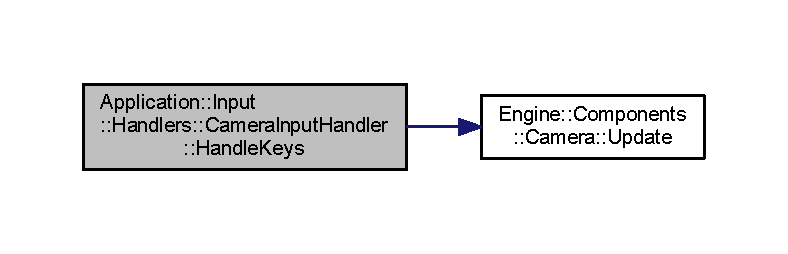
\includegraphics[width=350pt]{classApplication_1_1Input_1_1Handlers_1_1CameraInputHandler_a149884ea2dc9deea39d3dcd10dfa74b1_cgraph}
\end{center}
\end{figure}
\mbox{\Hypertarget{classApplication_1_1Input_1_1Handlers_1_1CameraInputHandler_ab06fa94ce5265dc06abb645ea29850bd}\label{classApplication_1_1Input_1_1Handlers_1_1CameraInputHandler_ab06fa94ce5265dc06abb645ea29850bd}} 
\index{Application\+::\+Input\+::\+Handlers\+::\+Camera\+Input\+Handler@{Application\+::\+Input\+::\+Handlers\+::\+Camera\+Input\+Handler}!Handle\+Mouse@{Handle\+Mouse}}
\index{Handle\+Mouse@{Handle\+Mouse}!Application\+::\+Input\+::\+Handlers\+::\+Camera\+Input\+Handler@{Application\+::\+Input\+::\+Handlers\+::\+Camera\+Input\+Handler}}
\subsubsection{\texorpdfstring{Handle\+Mouse()}{HandleMouse()}}
{\footnotesize\ttfamily bool Application\+::\+Input\+::\+Handlers\+::\+Camera\+Input\+Handler\+::\+Handle\+Mouse (\begin{DoxyParamCaption}\item[{\mbox{\hyperlink{classEngine_1_1BaseEngine}{Engine\+::\+Base\+Engine}} $\ast$}]{engine,  }\item[{\mbox{\hyperlink{classEngine_1_1Components_1_1Window}{Engine\+::\+Components\+::\+Window}} $\ast$}]{window,  }\item[{\mbox{\hyperlink{classEngine_1_1Components_1_1Scene}{Engine\+::\+Components\+::\+Scene}} $\ast$}]{scene,  }\item[{double}]{x,  }\item[{double}]{y,  }\item[{\mbox{\hyperlink{classGeneric_1_1Dictionary}{Generic\+::\+Dictionary}}$<$ short, bool $>$ \&}]{keys,  }\item[{int}]{keys\+Active }\end{DoxyParamCaption})\hspace{0.3cm}{\ttfamily [override]}}



Definition at line 53 of file Camera\+Input\+Handler.\+cpp.



References Engine\+::\+Components\+::\+Scene\+::\+Active\+Camera, Generic\+::\+Dictionary$<$ T\+Key, T\+Value $>$\+::\+Add(), Engine\+::\+Components\+::\+Camera\+::\+Direction, Generic\+::\+Dictionary$<$ T\+Key, T\+Value $>$\+::\+Get(), Engine\+::\+Components\+::\+Window\+::\+Height, M\+K\+\_\+R, Engine\+::\+Components\+::\+Scene\+::\+Objects, Engine\+::\+Base\+Engine\+::\+Programs, Engine\+::\+Components\+::\+Camera\+::\+Right, Engine\+::\+Base\+Engine\+::\+Shaders, sphere, Engine\+::\+Components\+::\+Camera\+::\+Up, Engine\+::\+Components\+::\+Camera\+::\+Update(), Engine\+::\+Components\+::\+Graphics\+::\+Material\+::\+Values, and Engine\+::\+Components\+::\+Window\+::\+Width.


\begin{DoxyCode}
54 \{
55     \textcolor{keywordflow}{if} (\mbox{\hyperlink{classApplication_1_1Input_1_1Handlers_1_1CameraInputHandler_ae8e329dd433afb42e5f53b5937a927fb}{\_lastMousePosition}}.x < 0)
56     \{
57         \mbox{\hyperlink{classApplication_1_1Input_1_1Handlers_1_1CameraInputHandler_ae8e329dd433afb42e5f53b5937a927fb}{\_lastMousePosition}}.x = x;
58         \mbox{\hyperlink{classApplication_1_1Input_1_1Handlers_1_1CameraInputHandler_ae8e329dd433afb42e5f53b5937a927fb}{\_lastMousePosition}}.y = y;
59     \}
60     \textcolor{comment}{// Allow Move mouse without camera change}
61     \textcolor{keywordflow}{if} (keys[\mbox{\hyperlink{IInputHandler_8h_a4cf9deae4ce7e88bc5a97b5678aa24d0}{MK\_R}}])
62     \{
63         \textcolor{keyword}{auto} fow = glm::radians(90.f);
64         \textcolor{keyword}{const} \textcolor{keywordtype}{float} sensitivity = 10.f;
65 
66         \textcolor{keyword}{auto} diff = glm::vec2(x, y) - \mbox{\hyperlink{classApplication_1_1Input_1_1Handlers_1_1CameraInputHandler_ae8e329dd433afb42e5f53b5937a927fb}{\_lastMousePosition}};
67         diff.x = diff.x * sensitivity * fow / \textcolor{keyword}{static\_cast<}\textcolor{keywordtype}{float}\textcolor{keyword}{>}(window->\mbox{\hyperlink{classEngine_1_1Components_1_1Window_ad5f71bfbb06ff5452b63bddf4b0c20b1}{Width}});
68         diff.y = diff.y * sensitivity * fow / \textcolor{keyword}{static\_cast<}\textcolor{keywordtype}{float}\textcolor{keyword}{>}(window->\mbox{\hyperlink{classEngine_1_1Components_1_1Window_ad9cf40200634bff27dbc7ae9a841bb99}{Height}});
69 
70         fprintf(stderr, \textcolor{stringliteral}{"Diff: %f, %f\(\backslash\)t"}, diff.x, diff.y);
71 
72         \textcolor{keywordflow}{if} (diff.x != 0 || diff.y != 0)
73         \{
74             *(scene->\mbox{\hyperlink{classEngine_1_1Components_1_1Scene_a9408befee37d89e2c001d25b9e4ed75a}{ActiveCamera}}->\mbox{\hyperlink{classEngine_1_1Components_1_1Camera_a23619a66046258f1158313f0c790ffa2}{Direction}}) += *(scene->
      \mbox{\hyperlink{classEngine_1_1Components_1_1Scene_a9408befee37d89e2c001d25b9e4ed75a}{ActiveCamera}}->\mbox{\hyperlink{classEngine_1_1Components_1_1Camera_a10b30289c89694d13918a979bade13d9}{Right}}) * diff.x;
75             *(scene->\mbox{\hyperlink{classEngine_1_1Components_1_1Scene_a9408befee37d89e2c001d25b9e4ed75a}{ActiveCamera}}->\mbox{\hyperlink{classEngine_1_1Components_1_1Camera_a23619a66046258f1158313f0c790ffa2}{Direction}}) -= *(scene->
      \mbox{\hyperlink{classEngine_1_1Components_1_1Scene_a9408befee37d89e2c001d25b9e4ed75a}{ActiveCamera}}->\mbox{\hyperlink{classEngine_1_1Components_1_1Camera_a84a4199b9c60579a0f148b9980e05200}{Up}}) * diff.y;
76             scene->\mbox{\hyperlink{classEngine_1_1Components_1_1Scene_a9408befee37d89e2c001d25b9e4ed75a}{ActiveCamera}}->\mbox{\hyperlink{classEngine_1_1Components_1_1Camera_a364f5e22921e3d234b31297a64c7d932}{Update}}();
77         \}
78     \}
79 
80     \textcolor{comment}{// Draw look point}
81     \textcolor{keyword}{auto} name = \textcolor{stringliteral}{"target"};
82     \textcolor{keyword}{auto} obj = scene->\mbox{\hyperlink{classEngine_1_1Components_1_1Scene_a23481feabaaa56bf5613765db03af4da}{Objects}}->\mbox{\hyperlink{classGeneric_1_1Dictionary_ad018bc166486129b48e9ededce313984}{Get}}(name);
83     \textcolor{keywordflow}{if} (obj == \textcolor{keyword}{nullptr})
84     \{
85 
86         \textcolor{keyword}{auto} mat = \textcolor{keyword}{new} \mbox{\hyperlink{classEngine_1_1Components_1_1Graphics_1_1Material}{Engine::Components::Graphics::Material}}(engine
      ->\mbox{\hyperlink{classEngine_1_1BaseEngine_ae0f86360ea3a384caefe443dd8f88601}{Programs}}->Get(\textcolor{stringliteral}{"basic"}));
87         mat->\mbox{\hyperlink{classEngine_1_1Components_1_1Graphics_1_1Material_a34335608ba1e6eb2c2dba5032107eab0}{Values}}->Add(\textcolor{keyword}{new} 
      \mbox{\hyperlink{classEngine_1_1Components_1_1Graphics_1_1MaterialValue}{Engine::Components::Graphics::MaterialValue<glm::vec4>}}
      (
88             engine->\mbox{\hyperlink{classEngine_1_1BaseEngine_a2582dee3f73da82bb422b43317b85e3b}{Shaders}}->Get(\textcolor{stringliteral}{"fragment"}), \textcolor{stringliteral}{"color"}, \textcolor{keyword}{new} glm::vec4(255.f, 0.f, 0.f, 1.f)
89         )).Add(\textcolor{keyword}{new} \mbox{\hyperlink{classEngine_1_1Components_1_1Graphics_1_1MaterialValue}{Engine::Components::Graphics::MaterialValue<bool>}}
      (
90             engine->\mbox{\hyperlink{classEngine_1_1BaseEngine_a2582dee3f73da82bb422b43317b85e3b}{Shaders}}->Get(\textcolor{stringliteral}{"fragment"}), \textcolor{stringliteral}{"useLighting"}, \textcolor{keyword}{new} bool(\textcolor{keyword}{false})
91         ));
92         \textcolor{keyword}{const} \textcolor{keyword}{auto} \textcolor{keywordtype}{object} = \textcolor{keyword}{new} \mbox{\hyperlink{classEngine_1_1Objects_1_1Sphere}{Engine::Objects::Sphere}}(mat, 
      \mbox{\hyperlink{2_2sphere_8h_a3663362197033eb86a9dcecea5a9d25f}{sphere}}, 17280, 3);
93         *(\textcolor{keywordtype}{object}->ModelMatrix) = glm::scale(glm::translate(glm::mat4(1.f), *scene->
      \mbox{\hyperlink{classEngine_1_1Components_1_1Scene_a9408befee37d89e2c001d25b9e4ed75a}{ActiveCamera}}->\mbox{\hyperlink{classEngine_1_1Components_1_1Camera_a23619a66046258f1158313f0c790ffa2}{Direction}}), glm::vec3(0.1f, 0.1f, 0.1f));
94         scene->\mbox{\hyperlink{classEngine_1_1Components_1_1Scene_a23481feabaaa56bf5613765db03af4da}{Objects}}->\mbox{\hyperlink{classGeneric_1_1Dictionary_ae7cb006f801b21c172e8fbac8794fa99}{Add}}(name, \textcolor{keywordtype}{object});
95     \}
96     \textcolor{keywordflow}{else}
97     \{
98         *(obj->ModelMatrix) = glm::scale(glm::translate(glm::mat4(1.f), *scene->
      \mbox{\hyperlink{classEngine_1_1Components_1_1Scene_a9408befee37d89e2c001d25b9e4ed75a}{ActiveCamera}}->\mbox{\hyperlink{classEngine_1_1Components_1_1Camera_a23619a66046258f1158313f0c790ffa2}{Direction}}), glm::vec3(0.1f, 0.1f, 0.1f));
99     \}
100 
101     \mbox{\hyperlink{classApplication_1_1Input_1_1Handlers_1_1CameraInputHandler_ae8e329dd433afb42e5f53b5937a927fb}{\_lastMousePosition}}.x = x;
102     \mbox{\hyperlink{classApplication_1_1Input_1_1Handlers_1_1CameraInputHandler_ae8e329dd433afb42e5f53b5937a927fb}{\_lastMousePosition}}.y = y;
103     \textcolor{keywordflow}{return} \textcolor{keyword}{true};
104 \}
\end{DoxyCode}
Here is the call graph for this function\+:
\nopagebreak
\begin{figure}[H]
\begin{center}
\leavevmode
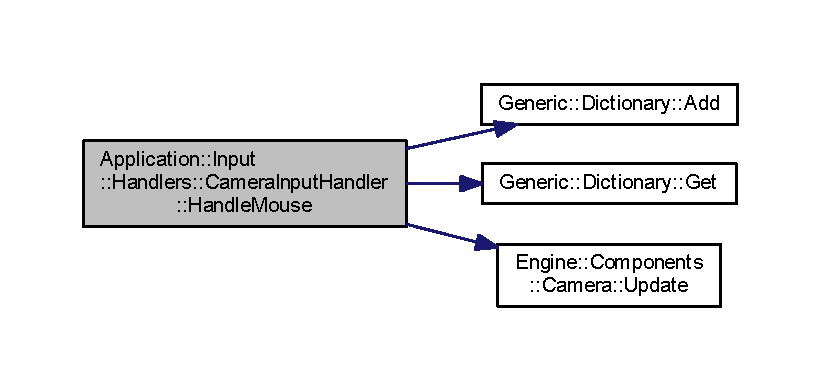
\includegraphics[width=350pt]{classApplication_1_1Input_1_1Handlers_1_1CameraInputHandler_ab06fa94ce5265dc06abb645ea29850bd_cgraph}
\end{center}
\end{figure}


\subsection{Member Data Documentation}
\mbox{\Hypertarget{classApplication_1_1Input_1_1Handlers_1_1CameraInputHandler_ae8e329dd433afb42e5f53b5937a927fb}\label{classApplication_1_1Input_1_1Handlers_1_1CameraInputHandler_ae8e329dd433afb42e5f53b5937a927fb}} 
\index{Application\+::\+Input\+::\+Handlers\+::\+Camera\+Input\+Handler@{Application\+::\+Input\+::\+Handlers\+::\+Camera\+Input\+Handler}!\+\_\+last\+Mouse\+Position@{\+\_\+last\+Mouse\+Position}}
\index{\+\_\+last\+Mouse\+Position@{\+\_\+last\+Mouse\+Position}!Application\+::\+Input\+::\+Handlers\+::\+Camera\+Input\+Handler@{Application\+::\+Input\+::\+Handlers\+::\+Camera\+Input\+Handler}}
\subsubsection{\texorpdfstring{\+\_\+last\+Mouse\+Position}{\_lastMousePosition}}
{\footnotesize\ttfamily glm\+::vec2 Application\+::\+Input\+::\+Handlers\+::\+Camera\+Input\+Handler\+::\+\_\+last\+Mouse\+Position\hspace{0.3cm}{\ttfamily [private]}}



Definition at line 14 of file Camera\+Input\+Handler.\+h.



Referenced by Camera\+Input\+Handler().

\mbox{\Hypertarget{classApplication_1_1Input_1_1Handlers_1_1CameraInputHandler_a0157ef737743b53e5db833012cd27372}\label{classApplication_1_1Input_1_1Handlers_1_1CameraInputHandler_a0157ef737743b53e5db833012cd27372}} 
\index{Application\+::\+Input\+::\+Handlers\+::\+Camera\+Input\+Handler@{Application\+::\+Input\+::\+Handlers\+::\+Camera\+Input\+Handler}!\+\_\+pitch@{\+\_\+pitch}}
\index{\+\_\+pitch@{\+\_\+pitch}!Application\+::\+Input\+::\+Handlers\+::\+Camera\+Input\+Handler@{Application\+::\+Input\+::\+Handlers\+::\+Camera\+Input\+Handler}}
\subsubsection{\texorpdfstring{\+\_\+pitch}{\_pitch}}
{\footnotesize\ttfamily float Application\+::\+Input\+::\+Handlers\+::\+Camera\+Input\+Handler\+::\+\_\+pitch\hspace{0.3cm}{\ttfamily [private]}}



Definition at line 15 of file Camera\+Input\+Handler.\+h.



Referenced by Camera\+Input\+Handler().

\mbox{\Hypertarget{classApplication_1_1Input_1_1Handlers_1_1CameraInputHandler_a2fa09dcae6ed67d452d374a9fb629349}\label{classApplication_1_1Input_1_1Handlers_1_1CameraInputHandler_a2fa09dcae6ed67d452d374a9fb629349}} 
\index{Application\+::\+Input\+::\+Handlers\+::\+Camera\+Input\+Handler@{Application\+::\+Input\+::\+Handlers\+::\+Camera\+Input\+Handler}!\+\_\+yaw@{\+\_\+yaw}}
\index{\+\_\+yaw@{\+\_\+yaw}!Application\+::\+Input\+::\+Handlers\+::\+Camera\+Input\+Handler@{Application\+::\+Input\+::\+Handlers\+::\+Camera\+Input\+Handler}}
\subsubsection{\texorpdfstring{\+\_\+yaw}{\_yaw}}
{\footnotesize\ttfamily float Application\+::\+Input\+::\+Handlers\+::\+Camera\+Input\+Handler\+::\+\_\+yaw\hspace{0.3cm}{\ttfamily [private]}}



Definition at line 16 of file Camera\+Input\+Handler.\+h.



Referenced by Camera\+Input\+Handler().



The documentation for this class was generated from the following files\+:\begin{DoxyCompactItemize}
\item 
Z\+P\+G/\mbox{\hyperlink{CameraInputHandler_8h}{Camera\+Input\+Handler.\+h}}\item 
Z\+P\+G/\mbox{\hyperlink{CameraInputHandler_8cpp}{Camera\+Input\+Handler.\+cpp}}\end{DoxyCompactItemize}

\hypertarget{classApplication_1_1Input_1_1Handlers_1_1LightingChangeInputHandler}{}\section{Application\+:\+:Input\+:\+:Handlers\+:\+:Lighting\+Change\+Input\+Handler Class Reference}
\label{classApplication_1_1Input_1_1Handlers_1_1LightingChangeInputHandler}\index{Application\+::\+Input\+::\+Handlers\+::\+Lighting\+Change\+Input\+Handler@{Application\+::\+Input\+::\+Handlers\+::\+Lighting\+Change\+Input\+Handler}}


{\ttfamily \#include $<$Lighting\+Change\+Input\+Handler.\+h$>$}



Inheritance diagram for Application\+:\+:Input\+:\+:Handlers\+:\+:Lighting\+Change\+Input\+Handler\+:
\nopagebreak
\begin{figure}[H]
\begin{center}
\leavevmode
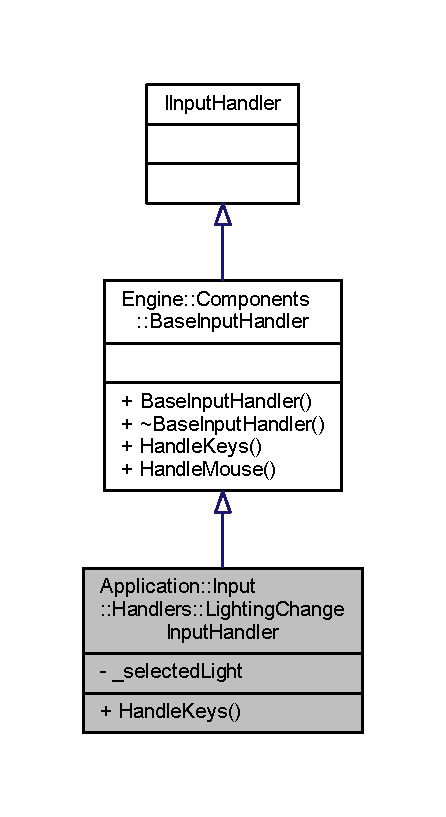
\includegraphics[width=214pt]{classApplication_1_1Input_1_1Handlers_1_1LightingChangeInputHandler__inherit__graph}
\end{center}
\end{figure}


Collaboration diagram for Application\+:\+:Input\+:\+:Handlers\+:\+:Lighting\+Change\+Input\+Handler\+:
\nopagebreak
\begin{figure}[H]
\begin{center}
\leavevmode
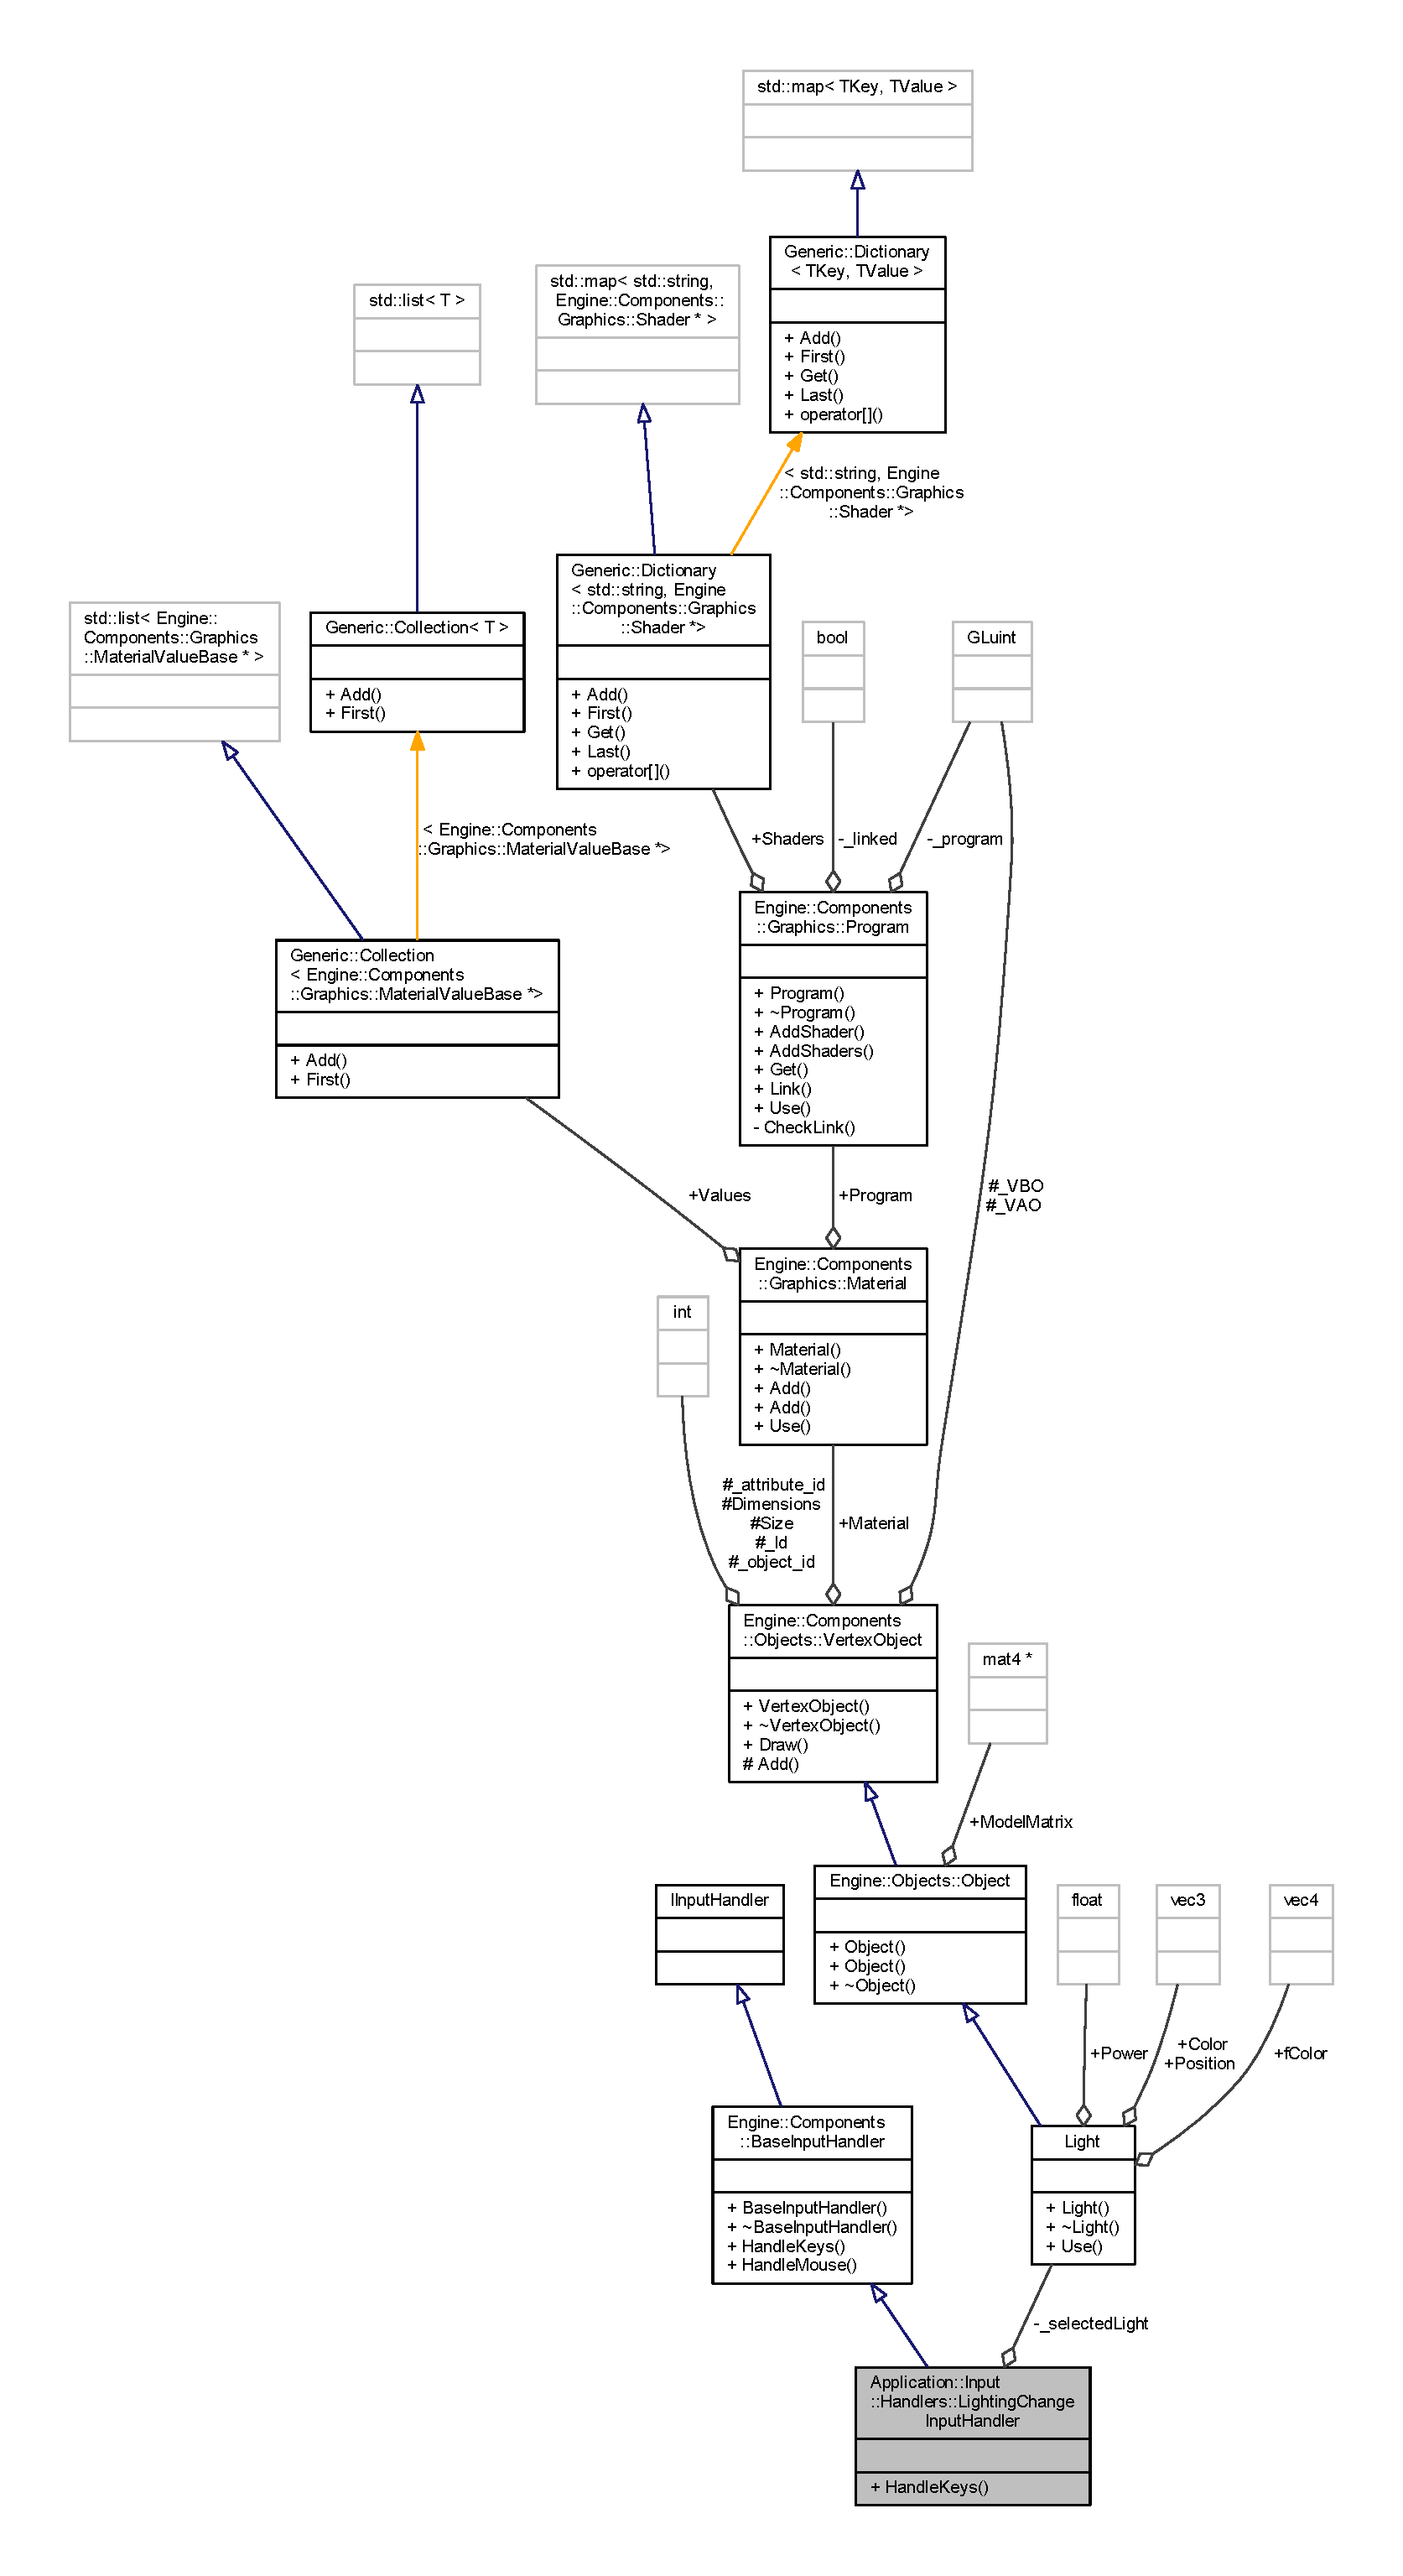
\includegraphics[height=550pt]{classApplication_1_1Input_1_1Handlers_1_1LightingChangeInputHandler__coll__graph}
\end{center}
\end{figure}
\subsection*{Public Member Functions}
\begin{DoxyCompactItemize}
\item 
bool \mbox{\hyperlink{classApplication_1_1Input_1_1Handlers_1_1LightingChangeInputHandler_a5017479d6edea9d6bedf3093cf49cb24}{Handle\+Keys}} (\mbox{\hyperlink{classEngine_1_1BaseEngine}{Engine\+::\+Base\+Engine}} $\ast$engine, \mbox{\hyperlink{classEngine_1_1Components_1_1Window}{Engine\+::\+Components\+::\+Window}} $\ast$window, \mbox{\hyperlink{classEngine_1_1Components_1_1Scene}{Engine\+::\+Components\+::\+Scene}} $\ast$scene, \mbox{\hyperlink{classGeneric_1_1Dictionary}{Generic\+::\+Dictionary}}$<$ short, bool $>$ \&keys, int keys\+Active) override
\item 
virtual bool \mbox{\hyperlink{classEngine_1_1Components_1_1BaseInputHandler_a8b50fb66d01573616072d708075a721e}{Handle\+Mouse}} (Base\+Engine $\ast$engine, Window $\ast$window, Scene $\ast$scene, double x, double y, \mbox{\hyperlink{classGeneric_1_1Dictionary}{Generic\+::\+Dictionary}}$<$ short, bool $>$ \&keys, int keys\+Active) override
\end{DoxyCompactItemize}
\subsection*{Private Attributes}
\begin{DoxyCompactItemize}
\item 
\mbox{\hyperlink{classLight}{Light}} $\ast$ \mbox{\hyperlink{classApplication_1_1Input_1_1Handlers_1_1LightingChangeInputHandler_a9d2d27b234fd09b3add304963534b719}{\+\_\+selected\+Light}} = nullptr
\end{DoxyCompactItemize}


\subsection{Detailed Description}


Definition at line 8 of file Lighting\+Change\+Input\+Handler.\+h.



\subsection{Member Function Documentation}
\mbox{\Hypertarget{classApplication_1_1Input_1_1Handlers_1_1LightingChangeInputHandler_a5017479d6edea9d6bedf3093cf49cb24}\label{classApplication_1_1Input_1_1Handlers_1_1LightingChangeInputHandler_a5017479d6edea9d6bedf3093cf49cb24}} 
\index{Application\+::\+Input\+::\+Handlers\+::\+Lighting\+Change\+Input\+Handler@{Application\+::\+Input\+::\+Handlers\+::\+Lighting\+Change\+Input\+Handler}!Handle\+Keys@{Handle\+Keys}}
\index{Handle\+Keys@{Handle\+Keys}!Application\+::\+Input\+::\+Handlers\+::\+Lighting\+Change\+Input\+Handler@{Application\+::\+Input\+::\+Handlers\+::\+Lighting\+Change\+Input\+Handler}}
\subsubsection{\texorpdfstring{Handle\+Keys()}{HandleKeys()}}
{\footnotesize\ttfamily bool Application\+::\+Input\+::\+Handlers\+::\+Lighting\+Change\+Input\+Handler\+::\+Handle\+Keys (\begin{DoxyParamCaption}\item[{\mbox{\hyperlink{classEngine_1_1BaseEngine}{Engine\+::\+Base\+Engine}} $\ast$}]{engine,  }\item[{\mbox{\hyperlink{classEngine_1_1Components_1_1Window}{Engine\+::\+Components\+::\+Window}} $\ast$}]{window,  }\item[{\mbox{\hyperlink{classEngine_1_1Components_1_1Scene}{Engine\+::\+Components\+::\+Scene}} $\ast$}]{scene,  }\item[{\mbox{\hyperlink{classGeneric_1_1Dictionary}{Generic\+::\+Dictionary}}$<$ short, bool $>$ \&}]{keys,  }\item[{int}]{keys\+Active }\end{DoxyParamCaption})\hspace{0.3cm}{\ttfamily [override]}, {\ttfamily [virtual]}}



Reimplemented from \mbox{\hyperlink{classEngine_1_1Components_1_1BaseInputHandler_af7deea3367074324fdbefe48119d40ce}{Engine\+::\+Components\+::\+Base\+Input\+Handler}}.



Definition at line 5 of file Lighting\+Change\+Input\+Handler.\+cpp.



References \+\_\+selected\+Light, Engine\+::\+Components\+::\+Scene\+::\+Active\+Camera, Generic\+::\+Dictionary$<$ T\+Key, T\+Value $>$\+::\+First(), Engine\+::\+Components\+::\+Scene\+::\+Lights, Engine\+::\+Objects\+::\+Object\+::\+Model\+Matrix, Light\+::\+Position, Light\+::\+Power, and Application\+::\+Engines\+::\+Light\+Engine\+::specular\+Size.


\begin{DoxyCode}
6 \{
7     \textcolor{keywordflow}{if}(keys[\textcolor{charliteral}{'L'}] && dynamic\_cast<Application::Engines::LightEngine*>(engine) != \textcolor{keyword}{nullptr})
8     \{
9         \textcolor{keywordflow}{if} (\mbox{\hyperlink{classApplication_1_1Input_1_1Handlers_1_1LightingChangeInputHandler_a9d2d27b234fd09b3add304963534b719}{\_selectedLight}} == \textcolor{keyword}{nullptr})
10             \mbox{\hyperlink{classApplication_1_1Input_1_1Handlers_1_1LightingChangeInputHandler_a9d2d27b234fd09b3add304963534b719}{\_selectedLight}} = scene->\mbox{\hyperlink{classEngine_1_1Components_1_1Scene_a00f60de2f6c72242a7af0076a3b75e5e}{Lights}}->\mbox{\hyperlink{classGeneric_1_1Dictionary_ab368d54de28e7a3514e1add4bb5b3a36}{First}}();
11         \textcolor{keyword}{auto} lightEngine = \textcolor{keyword}{dynamic\_cast<}\mbox{\hyperlink{classApplication_1_1Engines_1_1LightEngine}{Application::Engines::LightEngine}}*\textcolor{keyword}{
      >}(engine);
12 
13         \textcolor{keyword}{const} \textcolor{keyword}{auto} increment = (keys[\textcolor{charliteral}{'R'}] ? 1 : (keys[\textcolor{charliteral}{'F'}] ? -1 : 0));
14 
15         \textcolor{keywordflow}{if} (keys[\textcolor{charliteral}{'V'}])
16             lightEngine->\mbox{\hyperlink{classApplication_1_1Engines_1_1LightEngine_a5da28beed5c8d278c3615974d464f246}{specularSize}} += increment;
17         \textcolor{keywordflow}{if} (keys[\textcolor{charliteral}{'C'}])
18             lightEngine->specularStrength += increment * .005f;
19         \textcolor{keywordflow}{if} (keys[\textcolor{charliteral}{'X'}])
20             lightEngine->diffuseStrength += increment * .005f;
21         \textcolor{keywordflow}{if} (keys[\textcolor{charliteral}{'Z'}])
22             lightEngine->ambientStrength += increment * .001f;
23 
24         \textcolor{keywordflow}{if} (keys[\textcolor{charliteral}{'N'}])
25         \{
26             lightEngine->specularStrength = 0.f;
27             lightEngine->diffuseStrength = 0.f;
28             lightEngine->ambientStrength = 0.f;
29         \}
30         \textcolor{keywordflow}{if} (keys[\textcolor{charliteral}{'M'}])
31         \{
32             lightEngine->specularStrength = 0.5f;
33             lightEngine->diffuseStrength = 0.5f;
34             lightEngine->ambientStrength = 0.2f;
35         \}
36 
37         \textcolor{keyword}{const} \textcolor{keyword}{auto} camera = scene->\mbox{\hyperlink{classEngine_1_1Components_1_1Scene_a9408befee37d89e2c001d25b9e4ed75a}{ActiveCamera}};
38         \textcolor{keywordflow}{if} (increment != 0 && keysActive == 2)
39             \mbox{\hyperlink{classApplication_1_1Input_1_1Handlers_1_1LightingChangeInputHandler_a9d2d27b234fd09b3add304963534b719}{\_selectedLight}}->\mbox{\hyperlink{classLight_a161f4944da390d9bc388091bafd59fe3}{Power}} += increment * 0.01;
40 
41         \textcolor{keyword}{const} \textcolor{keywordtype}{float} speed = 0.2f;
42         \textcolor{keywordflow}{if} (keys[\textcolor{charliteral}{'W'}])
43             \mbox{\hyperlink{classApplication_1_1Input_1_1Handlers_1_1LightingChangeInputHandler_a9d2d27b234fd09b3add304963534b719}{\_selectedLight}}->\mbox{\hyperlink{classLight_ab6a04fde7b96f06ab935cd1d53b91e0b}{Position}} -= *(camera->Front) * speed;
44         \textcolor{keywordflow}{if} (keys[\textcolor{charliteral}{'S'}])
45             \mbox{\hyperlink{classApplication_1_1Input_1_1Handlers_1_1LightingChangeInputHandler_a9d2d27b234fd09b3add304963534b719}{\_selectedLight}}->\mbox{\hyperlink{classLight_ab6a04fde7b96f06ab935cd1d53b91e0b}{Position}} += *(camera->Front) * speed;
46         \textcolor{keywordflow}{if} (keys[\textcolor{charliteral}{'A'}])
47             \mbox{\hyperlink{classApplication_1_1Input_1_1Handlers_1_1LightingChangeInputHandler_a9d2d27b234fd09b3add304963534b719}{\_selectedLight}}->\mbox{\hyperlink{classLight_ab6a04fde7b96f06ab935cd1d53b91e0b}{Position}} -= *(camera->Right) * speed;
48         \textcolor{keywordflow}{if} (keys[\textcolor{charliteral}{'D'}])
49             \mbox{\hyperlink{classApplication_1_1Input_1_1Handlers_1_1LightingChangeInputHandler_a9d2d27b234fd09b3add304963534b719}{\_selectedLight}}->\mbox{\hyperlink{classLight_ab6a04fde7b96f06ab935cd1d53b91e0b}{Position}} += *(camera->Right) * speed;
50         \textcolor{keywordflow}{if} (keys[\textcolor{charliteral}{'E'}])
51             \mbox{\hyperlink{classApplication_1_1Input_1_1Handlers_1_1LightingChangeInputHandler_a9d2d27b234fd09b3add304963534b719}{\_selectedLight}}->\mbox{\hyperlink{classLight_ab6a04fde7b96f06ab935cd1d53b91e0b}{Position}} -= *(camera->Up) * speed;
52         \textcolor{keywordflow}{if} (keys[\textcolor{charliteral}{'Q'}])
53             \mbox{\hyperlink{classApplication_1_1Input_1_1Handlers_1_1LightingChangeInputHandler_a9d2d27b234fd09b3add304963534b719}{\_selectedLight}}->\mbox{\hyperlink{classLight_ab6a04fde7b96f06ab935cd1d53b91e0b}{Position}} += *(camera->Up) * speed;
54 
55         *\mbox{\hyperlink{classApplication_1_1Input_1_1Handlers_1_1LightingChangeInputHandler_a9d2d27b234fd09b3add304963534b719}{\_selectedLight}}->\mbox{\hyperlink{classEngine_1_1Objects_1_1Object_acf41cc091fa270053245ed26bc28c8a4}{ModelMatrix}} = glm::scale(
56             glm::translate(glm::mat4(1.f), \mbox{\hyperlink{classApplication_1_1Input_1_1Handlers_1_1LightingChangeInputHandler_a9d2d27b234fd09b3add304963534b719}{\_selectedLight}}->
      \mbox{\hyperlink{classLight_ab6a04fde7b96f06ab935cd1d53b91e0b}{Position}}), 
57             glm::vec3(0.2*\mbox{\hyperlink{classApplication_1_1Input_1_1Handlers_1_1LightingChangeInputHandler_a9d2d27b234fd09b3add304963534b719}{\_selectedLight}}->\mbox{\hyperlink{classLight_a161f4944da390d9bc388091bafd59fe3}{Power}}, 0.2*
      \mbox{\hyperlink{classApplication_1_1Input_1_1Handlers_1_1LightingChangeInputHandler_a9d2d27b234fd09b3add304963534b719}{\_selectedLight}}->\mbox{\hyperlink{classLight_a161f4944da390d9bc388091bafd59fe3}{Power}}, 0.2*\mbox{\hyperlink{classApplication_1_1Input_1_1Handlers_1_1LightingChangeInputHandler_a9d2d27b234fd09b3add304963534b719}{\_selectedLight}}->
      \mbox{\hyperlink{classLight_a161f4944da390d9bc388091bafd59fe3}{Power}})
58         );
59         \textcolor{keywordflow}{return} \textcolor{keyword}{false};
60     \}
61     \textcolor{keywordflow}{return} \textcolor{keyword}{true};
62 \}
\end{DoxyCode}
Here is the call graph for this function\+:
\nopagebreak
\begin{figure}[H]
\begin{center}
\leavevmode
\includegraphics[width=350pt]{classApplication_1_1Input_1_1Handlers_1_1LightingChangeInputHandler_a5017479d6edea9d6bedf3093cf49cb24_cgraph}
\end{center}
\end{figure}
\mbox{\Hypertarget{classEngine_1_1Components_1_1BaseInputHandler_a8b50fb66d01573616072d708075a721e}\label{classEngine_1_1Components_1_1BaseInputHandler_a8b50fb66d01573616072d708075a721e}} 
\index{Application\+::\+Input\+::\+Handlers\+::\+Lighting\+Change\+Input\+Handler@{Application\+::\+Input\+::\+Handlers\+::\+Lighting\+Change\+Input\+Handler}!Handle\+Mouse@{Handle\+Mouse}}
\index{Handle\+Mouse@{Handle\+Mouse}!Application\+::\+Input\+::\+Handlers\+::\+Lighting\+Change\+Input\+Handler@{Application\+::\+Input\+::\+Handlers\+::\+Lighting\+Change\+Input\+Handler}}
\subsubsection{\texorpdfstring{Handle\+Mouse()}{HandleMouse()}}
{\footnotesize\ttfamily bool Engine\+::\+Components\+::\+Base\+Input\+Handler\+::\+Handle\+Mouse (\begin{DoxyParamCaption}\item[{\mbox{\hyperlink{classEngine_1_1BaseEngine}{Base\+Engine}} $\ast$}]{engine,  }\item[{\mbox{\hyperlink{classEngine_1_1Components_1_1Window}{Window}} $\ast$}]{window,  }\item[{\mbox{\hyperlink{classEngine_1_1Components_1_1Scene}{Scene}} $\ast$}]{scene,  }\item[{double}]{x,  }\item[{double}]{y,  }\item[{\mbox{\hyperlink{classGeneric_1_1Dictionary}{Generic\+::\+Dictionary}}$<$ short, bool $>$ \&}]{keys,  }\item[{int}]{keys\+Active }\end{DoxyParamCaption})\hspace{0.3cm}{\ttfamily [override]}, {\ttfamily [virtual]}, {\ttfamily [inherited]}}



Definition at line 8 of file Base\+Input\+Handler.\+cpp.


\begin{DoxyCode}
9 \{
10     \textcolor{keywordflow}{return} \textcolor{keyword}{true};
11 \}
\end{DoxyCode}


\subsection{Member Data Documentation}
\mbox{\Hypertarget{classApplication_1_1Input_1_1Handlers_1_1LightingChangeInputHandler_a9d2d27b234fd09b3add304963534b719}\label{classApplication_1_1Input_1_1Handlers_1_1LightingChangeInputHandler_a9d2d27b234fd09b3add304963534b719}} 
\index{Application\+::\+Input\+::\+Handlers\+::\+Lighting\+Change\+Input\+Handler@{Application\+::\+Input\+::\+Handlers\+::\+Lighting\+Change\+Input\+Handler}!\+\_\+selected\+Light@{\+\_\+selected\+Light}}
\index{\+\_\+selected\+Light@{\+\_\+selected\+Light}!Application\+::\+Input\+::\+Handlers\+::\+Lighting\+Change\+Input\+Handler@{Application\+::\+Input\+::\+Handlers\+::\+Lighting\+Change\+Input\+Handler}}
\subsubsection{\texorpdfstring{\+\_\+selected\+Light}{\_selectedLight}}
{\footnotesize\ttfamily \mbox{\hyperlink{classLight}{Light}}$\ast$ Application\+::\+Input\+::\+Handlers\+::\+Lighting\+Change\+Input\+Handler\+::\+\_\+selected\+Light = nullptr\hspace{0.3cm}{\ttfamily [private]}}



Definition at line 13 of file Lighting\+Change\+Input\+Handler.\+h.



Referenced by Handle\+Keys().



The documentation for this class was generated from the following files\+:\begin{DoxyCompactItemize}
\item 
Z\+P\+G/\mbox{\hyperlink{LightingChangeInputHandler_8h}{Lighting\+Change\+Input\+Handler.\+h}}\item 
Z\+P\+G/\mbox{\hyperlink{LightingChangeInputHandler_8cpp}{Lighting\+Change\+Input\+Handler.\+cpp}}\end{DoxyCompactItemize}

\hypertarget{classApplication_1_1Scenes_1_1CameraScene}{}\section{Application\+:\+:Scenes\+:\+:Camera\+Scene Class Reference}
\label{classApplication_1_1Scenes_1_1CameraScene}\index{Application\+::\+Scenes\+::\+Camera\+Scene@{Application\+::\+Scenes\+::\+Camera\+Scene}}


{\ttfamily \#include $<$Camera\+Scene.\+h$>$}



Inheritance diagram for Application\+:\+:Scenes\+:\+:Camera\+Scene\+:
\nopagebreak
\begin{figure}[H]
\begin{center}
\leavevmode
\includegraphics[width=187pt]{classApplication_1_1Scenes_1_1CameraScene__inherit__graph}
\end{center}
\end{figure}


Collaboration diagram for Application\+:\+:Scenes\+:\+:Camera\+Scene\+:
\nopagebreak
\begin{figure}[H]
\begin{center}
\leavevmode
\includegraphics[width=350pt]{classApplication_1_1Scenes_1_1CameraScene__coll__graph}
\end{center}
\end{figure}
\subsection*{Public Member Functions}
\begin{DoxyCompactItemize}
\item 
\mbox{\hyperlink{classApplication_1_1Scenes_1_1CameraScene_a6276ab9be1ea87015c7508668e878edf}{Camera\+Scene}} ()
\item 
\mbox{\hyperlink{classApplication_1_1Scenes_1_1CameraScene_a7ae326096600efbfb172225cb53a0975}{$\sim$\+Camera\+Scene}} ()
\item 
virtual void \mbox{\hyperlink{classEngine_1_1Components_1_1Scene_af18bd334fe66952b8d79b8e9e99ab2d8}{Begin\+Load}} (Base\+Engine $\ast$engine)
\item 
void \mbox{\hyperlink{classApplication_1_1Scenes_1_1CameraScene_a92eb1a3eab4de7d18ca108e4aefd7fc7}{Frame\+Update}} (\mbox{\hyperlink{classEngine_1_1BaseEngine}{Engine\+::\+Base\+Engine}} $\ast$engine) override
\item 
void \mbox{\hyperlink{classApplication_1_1Scenes_1_1CameraScene_a86f30a60a125f491176ecfca46cd6b8a}{Load}} (\mbox{\hyperlink{classEngine_1_1BaseEngine}{Engine\+::\+Base\+Engine}} $\ast$engine) override
\item 
virtual void \mbox{\hyperlink{classEngine_1_1Components_1_1Scene_a936218df56c481f3aa12d684cee038f3}{Set\+Active\+Camera}} (Camera $\ast$camera=nullptr)
\item 
virtual void \mbox{\hyperlink{classEngine_1_1Components_1_1Scene_a064ce89da5daa483369c3253f04c9d21}{Unload}} (Base\+Engine $\ast$engine)
\end{DoxyCompactItemize}
\subsection*{Public Attributes}
\begin{DoxyCompactItemize}
\item 
Camera $\ast$ \mbox{\hyperlink{classEngine_1_1Components_1_1Scene_a9408befee37d89e2c001d25b9e4ed75a}{Active\+Camera}}
\item 
\mbox{\hyperlink{classGeneric_1_1Dictionary}{Generic\+::\+Dictionary}}$<$ std\+::string, Camera $\ast$ $>$ $\ast$ \mbox{\hyperlink{classEngine_1_1Components_1_1Scene_aea98ff1ced88ee859878b504e9a2a362}{Cameras}}
\item 
\mbox{\hyperlink{classGeneric_1_1Dictionary}{Generic\+::\+Dictionary}}$<$ std\+::string, \mbox{\hyperlink{classLight}{Light}} $\ast$ $>$ $\ast$ \mbox{\hyperlink{classEngine_1_1Components_1_1Scene_a00f60de2f6c72242a7af0076a3b75e5e}{Lights}}
\item 
\mbox{\hyperlink{classGeneric_1_1Dictionary}{Generic\+::\+Dictionary}}$<$ std\+::string, \mbox{\hyperlink{classEngine_1_1Objects_1_1Object}{Engine\+::\+Objects\+::\+Object}} $\ast$ $>$ $\ast$ \mbox{\hyperlink{classEngine_1_1Components_1_1Scene_a23481feabaaa56bf5613765db03af4da}{Objects}}
\end{DoxyCompactItemize}
\subsection*{Protected Attributes}
\begin{DoxyCompactItemize}
\item 
bool \mbox{\hyperlink{classEngine_1_1Components_1_1Scene_ae828757eea5410550f6674421051a783}{Loaded}}
\end{DoxyCompactItemize}
\subsection*{Private Attributes}
\begin{DoxyCompactItemize}
\item 
float $\ast$ \mbox{\hyperlink{classApplication_1_1Scenes_1_1CameraScene_a5b1ed7cbc9e95f0adf9f9ad9a9100d51}{angle}}
\item 
float $\ast$ \mbox{\hyperlink{classApplication_1_1Scenes_1_1CameraScene_a2ecbe017c52a0278302f8b8ffbc519ab}{color}}
\item 
glm\+::mat4 $\ast$ \mbox{\hyperlink{classApplication_1_1Scenes_1_1CameraScene_ac62c8a76d7ba9e9e25ec72d8513a46f4}{model\+Matrix}}
\end{DoxyCompactItemize}


\subsection{Detailed Description}


Definition at line 7 of file Camera\+Scene.\+h.



\subsection{Constructor \& Destructor Documentation}
\mbox{\Hypertarget{classApplication_1_1Scenes_1_1CameraScene_a6276ab9be1ea87015c7508668e878edf}\label{classApplication_1_1Scenes_1_1CameraScene_a6276ab9be1ea87015c7508668e878edf}} 
\index{Application\+::\+Scenes\+::\+Camera\+Scene@{Application\+::\+Scenes\+::\+Camera\+Scene}!Camera\+Scene@{Camera\+Scene}}
\index{Camera\+Scene@{Camera\+Scene}!Application\+::\+Scenes\+::\+Camera\+Scene@{Application\+::\+Scenes\+::\+Camera\+Scene}}
\subsubsection{\texorpdfstring{Camera\+Scene()}{CameraScene()}}
{\footnotesize\ttfamily Camera\+Scene\+::\+Camera\+Scene (\begin{DoxyParamCaption}{ }\end{DoxyParamCaption})}



Definition at line 5 of file Camera\+Scene.\+cpp.


\begin{DoxyCode}
6 \{
7 \}
\end{DoxyCode}
\mbox{\Hypertarget{classApplication_1_1Scenes_1_1CameraScene_a7ae326096600efbfb172225cb53a0975}\label{classApplication_1_1Scenes_1_1CameraScene_a7ae326096600efbfb172225cb53a0975}} 
\index{Application\+::\+Scenes\+::\+Camera\+Scene@{Application\+::\+Scenes\+::\+Camera\+Scene}!````~Camera\+Scene@{$\sim$\+Camera\+Scene}}
\index{````~Camera\+Scene@{$\sim$\+Camera\+Scene}!Application\+::\+Scenes\+::\+Camera\+Scene@{Application\+::\+Scenes\+::\+Camera\+Scene}}
\subsubsection{\texorpdfstring{$\sim$\+Camera\+Scene()}{~CameraScene()}}
{\footnotesize\ttfamily Camera\+Scene\+::$\sim$\+Camera\+Scene (\begin{DoxyParamCaption}{ }\end{DoxyParamCaption})}



Definition at line 10 of file Camera\+Scene.\+cpp.


\begin{DoxyCode}
11 \{
12 \}
\end{DoxyCode}


\subsection{Member Function Documentation}
\mbox{\Hypertarget{classEngine_1_1Components_1_1Scene_af18bd334fe66952b8d79b8e9e99ab2d8}\label{classEngine_1_1Components_1_1Scene_af18bd334fe66952b8d79b8e9e99ab2d8}} 
\index{Application\+::\+Scenes\+::\+Camera\+Scene@{Application\+::\+Scenes\+::\+Camera\+Scene}!Begin\+Load@{Begin\+Load}}
\index{Begin\+Load@{Begin\+Load}!Application\+::\+Scenes\+::\+Camera\+Scene@{Application\+::\+Scenes\+::\+Camera\+Scene}}
\subsubsection{\texorpdfstring{Begin\+Load()}{BeginLoad()}}
{\footnotesize\ttfamily void Engine\+::\+Components\+::\+Scene\+::\+Begin\+Load (\begin{DoxyParamCaption}\item[{\mbox{\hyperlink{classEngine_1_1BaseEngine}{Base\+Engine}} $\ast$}]{engine }\end{DoxyParamCaption})\hspace{0.3cm}{\ttfamily [virtual]}, {\ttfamily [inherited]}}



Definition at line 37 of file Scene.\+cpp.



Referenced by Application\+::\+Engines\+::\+Camera\+Engine\+::\+Init(), and Application\+::\+Engines\+::\+Light\+Engine\+::\+Init().


\begin{DoxyCode}
38 \{
39     \textcolor{keywordflow}{if} (!\mbox{\hyperlink{classEngine_1_1Components_1_1Scene_ae828757eea5410550f6674421051a783}{Loaded}})
40     \{
41         \mbox{\hyperlink{classEngine_1_1Components_1_1Scene_a23c5b23e66646443670a487e7c016e73}{Load}}(engine);
42         \textcolor{keywordflow}{if} (\mbox{\hyperlink{classEngine_1_1Components_1_1Scene_a9408befee37d89e2c001d25b9e4ed75a}{ActiveCamera}} == \textcolor{keyword}{nullptr})
43             \mbox{\hyperlink{classEngine_1_1Components_1_1Scene_a936218df56c481f3aa12d684cee038f3}{SetActiveCamera}}();
44         \mbox{\hyperlink{classEngine_1_1Components_1_1Scene_ae828757eea5410550f6674421051a783}{Loaded}} = \textcolor{keyword}{true};
45     \}
46 \}
\end{DoxyCode}
Here is the caller graph for this function\+:
\nopagebreak
\begin{figure}[H]
\begin{center}
\leavevmode
\includegraphics[width=329pt]{classEngine_1_1Components_1_1Scene_af18bd334fe66952b8d79b8e9e99ab2d8_icgraph}
\end{center}
\end{figure}
\mbox{\Hypertarget{classApplication_1_1Scenes_1_1CameraScene_a92eb1a3eab4de7d18ca108e4aefd7fc7}\label{classApplication_1_1Scenes_1_1CameraScene_a92eb1a3eab4de7d18ca108e4aefd7fc7}} 
\index{Application\+::\+Scenes\+::\+Camera\+Scene@{Application\+::\+Scenes\+::\+Camera\+Scene}!Frame\+Update@{Frame\+Update}}
\index{Frame\+Update@{Frame\+Update}!Application\+::\+Scenes\+::\+Camera\+Scene@{Application\+::\+Scenes\+::\+Camera\+Scene}}
\subsubsection{\texorpdfstring{Frame\+Update()}{FrameUpdate()}}
{\footnotesize\ttfamily void Application\+::\+Scenes\+::\+Camera\+Scene\+::\+Frame\+Update (\begin{DoxyParamCaption}\item[{\mbox{\hyperlink{classEngine_1_1BaseEngine}{Engine\+::\+Base\+Engine}} $\ast$}]{engine }\end{DoxyParamCaption})\hspace{0.3cm}{\ttfamily [override]}, {\ttfamily [virtual]}}



Reimplemented from \mbox{\hyperlink{classEngine_1_1Components_1_1Scene_abd8fcdcac52dbce6a0a18de3860ab087}{Engine\+::\+Components\+::\+Scene}}.

\mbox{\Hypertarget{classApplication_1_1Scenes_1_1CameraScene_a86f30a60a125f491176ecfca46cd6b8a}\label{classApplication_1_1Scenes_1_1CameraScene_a86f30a60a125f491176ecfca46cd6b8a}} 
\index{Application\+::\+Scenes\+::\+Camera\+Scene@{Application\+::\+Scenes\+::\+Camera\+Scene}!Load@{Load}}
\index{Load@{Load}!Application\+::\+Scenes\+::\+Camera\+Scene@{Application\+::\+Scenes\+::\+Camera\+Scene}}
\subsubsection{\texorpdfstring{Load()}{Load()}}
{\footnotesize\ttfamily void Application\+::\+Scenes\+::\+Camera\+Scene\+::\+Load (\begin{DoxyParamCaption}\item[{\mbox{\hyperlink{classEngine_1_1BaseEngine}{Engine\+::\+Base\+Engine}} $\ast$}]{engine }\end{DoxyParamCaption})\hspace{0.3cm}{\ttfamily [override]}, {\ttfamily [virtual]}}



Reimplemented from \mbox{\hyperlink{classEngine_1_1Components_1_1Scene_a23c5b23e66646443670a487e7c016e73}{Engine\+::\+Components\+::\+Scene}}.

\mbox{\Hypertarget{classEngine_1_1Components_1_1Scene_a936218df56c481f3aa12d684cee038f3}\label{classEngine_1_1Components_1_1Scene_a936218df56c481f3aa12d684cee038f3}} 
\index{Application\+::\+Scenes\+::\+Camera\+Scene@{Application\+::\+Scenes\+::\+Camera\+Scene}!Set\+Active\+Camera@{Set\+Active\+Camera}}
\index{Set\+Active\+Camera@{Set\+Active\+Camera}!Application\+::\+Scenes\+::\+Camera\+Scene@{Application\+::\+Scenes\+::\+Camera\+Scene}}
\subsubsection{\texorpdfstring{Set\+Active\+Camera()}{SetActiveCamera()}}
{\footnotesize\ttfamily void Engine\+::\+Components\+::\+Scene\+::\+Set\+Active\+Camera (\begin{DoxyParamCaption}\item[{\mbox{\hyperlink{classEngine_1_1Components_1_1Camera}{Camera}} $\ast$}]{camera = {\ttfamily nullptr} }\end{DoxyParamCaption})\hspace{0.3cm}{\ttfamily [virtual]}, {\ttfamily [inherited]}}



Definition at line 52 of file Scene.\+cpp.



References Engine\+::\+Components\+::\+Camera\+::\+Update().



Referenced by Engine\+::\+Components\+::\+Camera\+::\+Set\+Active().


\begin{DoxyCode}
53 \{
54     \textcolor{keywordflow}{if} (camera == \textcolor{keyword}{nullptr})
55         \mbox{\hyperlink{classEngine_1_1Components_1_1Scene_a9408befee37d89e2c001d25b9e4ed75a}{ActiveCamera}} = \mbox{\hyperlink{classEngine_1_1Components_1_1Scene_aea98ff1ced88ee859878b504e9a2a362}{Cameras}}->First();
56     \textcolor{keywordflow}{else}
57         \mbox{\hyperlink{classEngine_1_1Components_1_1Scene_a9408befee37d89e2c001d25b9e4ed75a}{ActiveCamera}} = camera;
58     \textcolor{keywordflow}{if}(\mbox{\hyperlink{classEngine_1_1Components_1_1Scene_a9408befee37d89e2c001d25b9e4ed75a}{ActiveCamera}} != \textcolor{keyword}{nullptr})
59         \mbox{\hyperlink{classEngine_1_1Components_1_1Scene_a9408befee37d89e2c001d25b9e4ed75a}{ActiveCamera}}->\mbox{\hyperlink{classEngine_1_1Components_1_1Camera_a364f5e22921e3d234b31297a64c7d932}{Update}}();
60 \}
\end{DoxyCode}
Here is the call graph for this function\+:
\nopagebreak
\begin{figure}[H]
\begin{center}
\leavevmode
\includegraphics[width=350pt]{classEngine_1_1Components_1_1Scene_a936218df56c481f3aa12d684cee038f3_cgraph}
\end{center}
\end{figure}
Here is the caller graph for this function\+:
\nopagebreak
\begin{figure}[H]
\begin{center}
\leavevmode
\includegraphics[width=350pt]{classEngine_1_1Components_1_1Scene_a936218df56c481f3aa12d684cee038f3_icgraph}
\end{center}
\end{figure}
\mbox{\Hypertarget{classEngine_1_1Components_1_1Scene_a064ce89da5daa483369c3253f04c9d21}\label{classEngine_1_1Components_1_1Scene_a064ce89da5daa483369c3253f04c9d21}} 
\index{Application\+::\+Scenes\+::\+Camera\+Scene@{Application\+::\+Scenes\+::\+Camera\+Scene}!Unload@{Unload}}
\index{Unload@{Unload}!Application\+::\+Scenes\+::\+Camera\+Scene@{Application\+::\+Scenes\+::\+Camera\+Scene}}
\subsubsection{\texorpdfstring{Unload()}{Unload()}}
{\footnotesize\ttfamily void Engine\+::\+Components\+::\+Scene\+::\+Unload (\begin{DoxyParamCaption}\item[{\mbox{\hyperlink{classEngine_1_1BaseEngine}{Base\+Engine}} $\ast$}]{engine }\end{DoxyParamCaption})\hspace{0.3cm}{\ttfamily [virtual]}, {\ttfamily [inherited]}}



Definition at line 29 of file Scene.\+cpp.


\begin{DoxyCode}
30 \{
31     \textcolor{keywordflow}{for} (\textcolor{keyword}{auto}& Object : *\mbox{\hyperlink{classEngine_1_1Components_1_1Scene_a23481feabaaa56bf5613765db03af4da}{Objects}})
32         \textcolor{keyword}{delete} Object.second;
33     \mbox{\hyperlink{classEngine_1_1Components_1_1Scene_a23481feabaaa56bf5613765db03af4da}{Objects}}->clear();
34     \mbox{\hyperlink{classEngine_1_1Components_1_1Scene_ae828757eea5410550f6674421051a783}{Loaded}} = \textcolor{keyword}{false};
35 \}
\end{DoxyCode}


\subsection{Member Data Documentation}
\mbox{\Hypertarget{classEngine_1_1Components_1_1Scene_a9408befee37d89e2c001d25b9e4ed75a}\label{classEngine_1_1Components_1_1Scene_a9408befee37d89e2c001d25b9e4ed75a}} 
\index{Application\+::\+Scenes\+::\+Camera\+Scene@{Application\+::\+Scenes\+::\+Camera\+Scene}!Active\+Camera@{Active\+Camera}}
\index{Active\+Camera@{Active\+Camera}!Application\+::\+Scenes\+::\+Camera\+Scene@{Application\+::\+Scenes\+::\+Camera\+Scene}}
\subsubsection{\texorpdfstring{Active\+Camera}{ActiveCamera}}
{\footnotesize\ttfamily Camera$\ast$ Engine\+::\+Components\+::\+Scene\+::\+Active\+Camera\hspace{0.3cm}{\ttfamily [inherited]}}



Definition at line 30 of file Scene.\+h.



Referenced by Application\+::\+Input\+::\+Handlers\+::\+Lighting\+Change\+Input\+Handler\+::\+Handle\+Keys(), Application\+::\+Input\+::\+Handlers\+::\+Camera\+Input\+Handler\+::\+Handle\+Keys(), Application\+::\+Input\+::\+Handlers\+::\+Camera\+Input\+Handler\+::\+Handle\+Mouse(), Application\+::\+Engines\+::\+Light\+Engine\+::\+Init(), and Engine\+::\+Components\+::\+Scene\+::\+Scene().

\mbox{\Hypertarget{classApplication_1_1Scenes_1_1CameraScene_a5b1ed7cbc9e95f0adf9f9ad9a9100d51}\label{classApplication_1_1Scenes_1_1CameraScene_a5b1ed7cbc9e95f0adf9f9ad9a9100d51}} 
\index{Application\+::\+Scenes\+::\+Camera\+Scene@{Application\+::\+Scenes\+::\+Camera\+Scene}!angle@{angle}}
\index{angle@{angle}!Application\+::\+Scenes\+::\+Camera\+Scene@{Application\+::\+Scenes\+::\+Camera\+Scene}}
\subsubsection{\texorpdfstring{angle}{angle}}
{\footnotesize\ttfamily float$\ast$ Application\+::\+Scenes\+::\+Camera\+Scene\+::angle\hspace{0.3cm}{\ttfamily [private]}}



Definition at line 16 of file Camera\+Scene.\+h.

\mbox{\Hypertarget{classEngine_1_1Components_1_1Scene_aea98ff1ced88ee859878b504e9a2a362}\label{classEngine_1_1Components_1_1Scene_aea98ff1ced88ee859878b504e9a2a362}} 
\index{Application\+::\+Scenes\+::\+Camera\+Scene@{Application\+::\+Scenes\+::\+Camera\+Scene}!Cameras@{Cameras}}
\index{Cameras@{Cameras}!Application\+::\+Scenes\+::\+Camera\+Scene@{Application\+::\+Scenes\+::\+Camera\+Scene}}
\subsubsection{\texorpdfstring{Cameras}{Cameras}}
{\footnotesize\ttfamily \mbox{\hyperlink{classGeneric_1_1Dictionary}{Generic\+::\+Dictionary}}$<$std\+::string, Camera$\ast$$>$$\ast$ Engine\+::\+Components\+::\+Scene\+::\+Cameras\hspace{0.3cm}{\ttfamily [inherited]}}



Definition at line 28 of file Scene.\+h.



Referenced by Application\+::\+Engines\+::\+Camera\+Engine\+::\+Init(), Application\+::\+Engines\+::\+Light\+Engine\+::\+Init(), and Engine\+::\+Components\+::\+Scene\+::\+Scene().

\mbox{\Hypertarget{classApplication_1_1Scenes_1_1CameraScene_a2ecbe017c52a0278302f8b8ffbc519ab}\label{classApplication_1_1Scenes_1_1CameraScene_a2ecbe017c52a0278302f8b8ffbc519ab}} 
\index{Application\+::\+Scenes\+::\+Camera\+Scene@{Application\+::\+Scenes\+::\+Camera\+Scene}!color@{color}}
\index{color@{color}!Application\+::\+Scenes\+::\+Camera\+Scene@{Application\+::\+Scenes\+::\+Camera\+Scene}}
\subsubsection{\texorpdfstring{color}{color}}
{\footnotesize\ttfamily float$\ast$ Application\+::\+Scenes\+::\+Camera\+Scene\+::color\hspace{0.3cm}{\ttfamily [private]}}



Definition at line 17 of file Camera\+Scene.\+h.

\mbox{\Hypertarget{classEngine_1_1Components_1_1Scene_a00f60de2f6c72242a7af0076a3b75e5e}\label{classEngine_1_1Components_1_1Scene_a00f60de2f6c72242a7af0076a3b75e5e}} 
\index{Application\+::\+Scenes\+::\+Camera\+Scene@{Application\+::\+Scenes\+::\+Camera\+Scene}!Lights@{Lights}}
\index{Lights@{Lights}!Application\+::\+Scenes\+::\+Camera\+Scene@{Application\+::\+Scenes\+::\+Camera\+Scene}}
\subsubsection{\texorpdfstring{Lights}{Lights}}
{\footnotesize\ttfamily \mbox{\hyperlink{classGeneric_1_1Dictionary}{Generic\+::\+Dictionary}}$<$std\+::string, \mbox{\hyperlink{classLight}{Light}}$\ast$$>$$\ast$ Engine\+::\+Components\+::\+Scene\+::\+Lights\hspace{0.3cm}{\ttfamily [inherited]}}



Definition at line 29 of file Scene.\+h.



Referenced by Application\+::\+Input\+::\+Handlers\+::\+Lighting\+Change\+Input\+Handler\+::\+Handle\+Keys(), Application\+::\+Engines\+::\+Light\+Engine\+::\+Init(), and Engine\+::\+Components\+::\+Scene\+::\+Scene().

\mbox{\Hypertarget{classEngine_1_1Components_1_1Scene_ae828757eea5410550f6674421051a783}\label{classEngine_1_1Components_1_1Scene_ae828757eea5410550f6674421051a783}} 
\index{Application\+::\+Scenes\+::\+Camera\+Scene@{Application\+::\+Scenes\+::\+Camera\+Scene}!Loaded@{Loaded}}
\index{Loaded@{Loaded}!Application\+::\+Scenes\+::\+Camera\+Scene@{Application\+::\+Scenes\+::\+Camera\+Scene}}
\subsubsection{\texorpdfstring{Loaded}{Loaded}}
{\footnotesize\ttfamily bool Engine\+::\+Components\+::\+Scene\+::\+Loaded\hspace{0.3cm}{\ttfamily [protected]}, {\ttfamily [inherited]}}



Definition at line 18 of file Scene.\+h.



Referenced by Engine\+::\+Components\+::\+Scene\+::\+Scene().

\mbox{\Hypertarget{classApplication_1_1Scenes_1_1CameraScene_ac62c8a76d7ba9e9e25ec72d8513a46f4}\label{classApplication_1_1Scenes_1_1CameraScene_ac62c8a76d7ba9e9e25ec72d8513a46f4}} 
\index{Application\+::\+Scenes\+::\+Camera\+Scene@{Application\+::\+Scenes\+::\+Camera\+Scene}!model\+Matrix@{model\+Matrix}}
\index{model\+Matrix@{model\+Matrix}!Application\+::\+Scenes\+::\+Camera\+Scene@{Application\+::\+Scenes\+::\+Camera\+Scene}}
\subsubsection{\texorpdfstring{model\+Matrix}{modelMatrix}}
{\footnotesize\ttfamily glm\+::mat4$\ast$ Application\+::\+Scenes\+::\+Camera\+Scene\+::model\+Matrix\hspace{0.3cm}{\ttfamily [private]}}



Definition at line 15 of file Camera\+Scene.\+h.

\mbox{\Hypertarget{classEngine_1_1Components_1_1Scene_a23481feabaaa56bf5613765db03af4da}\label{classEngine_1_1Components_1_1Scene_a23481feabaaa56bf5613765db03af4da}} 
\index{Application\+::\+Scenes\+::\+Camera\+Scene@{Application\+::\+Scenes\+::\+Camera\+Scene}!Objects@{Objects}}
\index{Objects@{Objects}!Application\+::\+Scenes\+::\+Camera\+Scene@{Application\+::\+Scenes\+::\+Camera\+Scene}}
\subsubsection{\texorpdfstring{Objects}{Objects}}
{\footnotesize\ttfamily \mbox{\hyperlink{classGeneric_1_1Dictionary}{Generic\+::\+Dictionary}}$<$std\+::string, \mbox{\hyperlink{classEngine_1_1Objects_1_1Object}{Engine\+::\+Objects\+::\+Object}}$\ast$$>$$\ast$ Engine\+::\+Components\+::\+Scene\+::\+Objects\hspace{0.3cm}{\ttfamily [inherited]}}



Definition at line 27 of file Scene.\+h.



Referenced by Application\+::\+Input\+::\+Handlers\+::\+Camera\+Input\+Handler\+::\+Handle\+Mouse(), Application\+::\+Engines\+::\+Camera\+Engine\+::\+Init(), Application\+::\+Engines\+::\+Light\+Engine\+::\+Init(), and Engine\+::\+Components\+::\+Scene\+::\+Scene().



The documentation for this class was generated from the following files\+:\begin{DoxyCompactItemize}
\item 
Z\+P\+G/\mbox{\hyperlink{CameraScene_8h}{Camera\+Scene.\+h}}\item 
Z\+P\+G/\mbox{\hyperlink{CameraScene_8cpp}{Camera\+Scene.\+cpp}}\end{DoxyCompactItemize}

\hypertarget{classApplication_1_1Scenes_1_1SphereScene}{}\section{Application\+:\+:Scenes\+:\+:Sphere\+Scene Class Reference}
\label{classApplication_1_1Scenes_1_1SphereScene}\index{Application\+::\+Scenes\+::\+Sphere\+Scene@{Application\+::\+Scenes\+::\+Sphere\+Scene}}


{\ttfamily \#include $<$Sphere\+Scene.\+h$>$}



Inheritance diagram for Application\+:\+:Scenes\+:\+:Sphere\+Scene\+:
\nopagebreak
\begin{figure}[H]
\begin{center}
\leavevmode
\includegraphics[width=187pt]{classApplication_1_1Scenes_1_1SphereScene__inherit__graph}
\end{center}
\end{figure}


Collaboration diagram for Application\+:\+:Scenes\+:\+:Sphere\+Scene\+:
\nopagebreak
\begin{figure}[H]
\begin{center}
\leavevmode
\includegraphics[width=350pt]{classApplication_1_1Scenes_1_1SphereScene__coll__graph}
\end{center}
\end{figure}
\subsection*{Public Member Functions}
\begin{DoxyCompactItemize}
\item 
\mbox{\hyperlink{classApplication_1_1Scenes_1_1SphereScene_a5880969092c7164e61a4236860c121c1}{Sphere\+Scene}} ()
\item 
\mbox{\hyperlink{classApplication_1_1Scenes_1_1SphereScene_a36617ce2362ace6514125d71d2fe41a9}{$\sim$\+Sphere\+Scene}} ()
\item 
virtual void \mbox{\hyperlink{classEngine_1_1Components_1_1Scene_af18bd334fe66952b8d79b8e9e99ab2d8}{Begin\+Load}} (Base\+Engine $\ast$engine)
\item 
void \mbox{\hyperlink{classApplication_1_1Scenes_1_1SphereScene_ad754dea94c77524a79d707436a933c66}{Frame\+Update}} (\mbox{\hyperlink{classEngine_1_1BaseEngine}{Engine\+::\+Base\+Engine}} $\ast$engine) override
\item 
void \mbox{\hyperlink{classApplication_1_1Scenes_1_1SphereScene_adf6f95bf2ac8f0e84935d04248407ba4}{Load}} (\mbox{\hyperlink{classEngine_1_1BaseEngine}{Engine\+::\+Base\+Engine}} $\ast$engine) override
\item 
virtual void \mbox{\hyperlink{classEngine_1_1Components_1_1Scene_a936218df56c481f3aa12d684cee038f3}{Set\+Active\+Camera}} (Camera $\ast$camera=nullptr)
\item 
virtual void \mbox{\hyperlink{classEngine_1_1Components_1_1Scene_a064ce89da5daa483369c3253f04c9d21}{Unload}} (Base\+Engine $\ast$engine)
\end{DoxyCompactItemize}
\subsection*{Public Attributes}
\begin{DoxyCompactItemize}
\item 
Camera $\ast$ \mbox{\hyperlink{classEngine_1_1Components_1_1Scene_a9408befee37d89e2c001d25b9e4ed75a}{Active\+Camera}}
\item 
\mbox{\hyperlink{classGeneric_1_1Dictionary}{Generic\+::\+Dictionary}}$<$ std\+::string, Camera $\ast$ $>$ $\ast$ \mbox{\hyperlink{classEngine_1_1Components_1_1Scene_aea98ff1ced88ee859878b504e9a2a362}{Cameras}}
\item 
\mbox{\hyperlink{classGeneric_1_1Dictionary}{Generic\+::\+Dictionary}}$<$ std\+::string, \mbox{\hyperlink{classLight}{Light}} $\ast$ $>$ $\ast$ \mbox{\hyperlink{classEngine_1_1Components_1_1Scene_a00f60de2f6c72242a7af0076a3b75e5e}{Lights}}
\item 
\mbox{\hyperlink{classGeneric_1_1Dictionary}{Generic\+::\+Dictionary}}$<$ std\+::string, \mbox{\hyperlink{classEngine_1_1Objects_1_1Object}{Engine\+::\+Objects\+::\+Object}} $\ast$ $>$ $\ast$ \mbox{\hyperlink{classEngine_1_1Components_1_1Scene_a23481feabaaa56bf5613765db03af4da}{Objects}}
\end{DoxyCompactItemize}
\subsection*{Protected Attributes}
\begin{DoxyCompactItemize}
\item 
bool \mbox{\hyperlink{classEngine_1_1Components_1_1Scene_ae828757eea5410550f6674421051a783}{Loaded}}
\end{DoxyCompactItemize}


\subsection{Detailed Description}


Definition at line 8 of file Sphere\+Scene.\+h.



\subsection{Constructor \& Destructor Documentation}
\mbox{\Hypertarget{classApplication_1_1Scenes_1_1SphereScene_a5880969092c7164e61a4236860c121c1}\label{classApplication_1_1Scenes_1_1SphereScene_a5880969092c7164e61a4236860c121c1}} 
\index{Application\+::\+Scenes\+::\+Sphere\+Scene@{Application\+::\+Scenes\+::\+Sphere\+Scene}!Sphere\+Scene@{Sphere\+Scene}}
\index{Sphere\+Scene@{Sphere\+Scene}!Application\+::\+Scenes\+::\+Sphere\+Scene@{Application\+::\+Scenes\+::\+Sphere\+Scene}}
\subsubsection{\texorpdfstring{Sphere\+Scene()}{SphereScene()}}
{\footnotesize\ttfamily Application\+::\+Scenes\+::\+Sphere\+Scene\+::\+Sphere\+Scene (\begin{DoxyParamCaption}{ }\end{DoxyParamCaption})}



Definition at line 9 of file Sphere\+Scene.\+cpp.


\begin{DoxyCode}
10 \{
11 \}
\end{DoxyCode}
\mbox{\Hypertarget{classApplication_1_1Scenes_1_1SphereScene_a36617ce2362ace6514125d71d2fe41a9}\label{classApplication_1_1Scenes_1_1SphereScene_a36617ce2362ace6514125d71d2fe41a9}} 
\index{Application\+::\+Scenes\+::\+Sphere\+Scene@{Application\+::\+Scenes\+::\+Sphere\+Scene}!````~Sphere\+Scene@{$\sim$\+Sphere\+Scene}}
\index{````~Sphere\+Scene@{$\sim$\+Sphere\+Scene}!Application\+::\+Scenes\+::\+Sphere\+Scene@{Application\+::\+Scenes\+::\+Sphere\+Scene}}
\subsubsection{\texorpdfstring{$\sim$\+Sphere\+Scene()}{~SphereScene()}}
{\footnotesize\ttfamily Application\+::\+Scenes\+::\+Sphere\+Scene\+::$\sim$\+Sphere\+Scene (\begin{DoxyParamCaption}{ }\end{DoxyParamCaption})}



Definition at line 13 of file Sphere\+Scene.\+cpp.


\begin{DoxyCode}
14 \{
15     Scene::~Scene();
16 \}
\end{DoxyCode}


\subsection{Member Function Documentation}
\mbox{\Hypertarget{classEngine_1_1Components_1_1Scene_af18bd334fe66952b8d79b8e9e99ab2d8}\label{classEngine_1_1Components_1_1Scene_af18bd334fe66952b8d79b8e9e99ab2d8}} 
\index{Application\+::\+Scenes\+::\+Sphere\+Scene@{Application\+::\+Scenes\+::\+Sphere\+Scene}!Begin\+Load@{Begin\+Load}}
\index{Begin\+Load@{Begin\+Load}!Application\+::\+Scenes\+::\+Sphere\+Scene@{Application\+::\+Scenes\+::\+Sphere\+Scene}}
\subsubsection{\texorpdfstring{Begin\+Load()}{BeginLoad()}}
{\footnotesize\ttfamily void Engine\+::\+Components\+::\+Scene\+::\+Begin\+Load (\begin{DoxyParamCaption}\item[{\mbox{\hyperlink{classEngine_1_1BaseEngine}{Base\+Engine}} $\ast$}]{engine }\end{DoxyParamCaption})\hspace{0.3cm}{\ttfamily [virtual]}, {\ttfamily [inherited]}}



Definition at line 37 of file Scene.\+cpp.



Referenced by Application\+::\+Engines\+::\+Camera\+Engine\+::\+Init(), and Application\+::\+Engines\+::\+Light\+Engine\+::\+Init().


\begin{DoxyCode}
38 \{
39     \textcolor{keywordflow}{if} (!\mbox{\hyperlink{classEngine_1_1Components_1_1Scene_ae828757eea5410550f6674421051a783}{Loaded}})
40     \{
41         \mbox{\hyperlink{classEngine_1_1Components_1_1Scene_a23c5b23e66646443670a487e7c016e73}{Load}}(engine);
42         \textcolor{keywordflow}{if} (\mbox{\hyperlink{classEngine_1_1Components_1_1Scene_a9408befee37d89e2c001d25b9e4ed75a}{ActiveCamera}} == \textcolor{keyword}{nullptr})
43             \mbox{\hyperlink{classEngine_1_1Components_1_1Scene_a936218df56c481f3aa12d684cee038f3}{SetActiveCamera}}();
44         \mbox{\hyperlink{classEngine_1_1Components_1_1Scene_ae828757eea5410550f6674421051a783}{Loaded}} = \textcolor{keyword}{true};
45     \}
46 \}
\end{DoxyCode}
Here is the caller graph for this function\+:
\nopagebreak
\begin{figure}[H]
\begin{center}
\leavevmode
\includegraphics[width=329pt]{classEngine_1_1Components_1_1Scene_af18bd334fe66952b8d79b8e9e99ab2d8_icgraph}
\end{center}
\end{figure}
\mbox{\Hypertarget{classApplication_1_1Scenes_1_1SphereScene_ad754dea94c77524a79d707436a933c66}\label{classApplication_1_1Scenes_1_1SphereScene_ad754dea94c77524a79d707436a933c66}} 
\index{Application\+::\+Scenes\+::\+Sphere\+Scene@{Application\+::\+Scenes\+::\+Sphere\+Scene}!Frame\+Update@{Frame\+Update}}
\index{Frame\+Update@{Frame\+Update}!Application\+::\+Scenes\+::\+Sphere\+Scene@{Application\+::\+Scenes\+::\+Sphere\+Scene}}
\subsubsection{\texorpdfstring{Frame\+Update()}{FrameUpdate()}}
{\footnotesize\ttfamily void Application\+::\+Scenes\+::\+Sphere\+Scene\+::\+Frame\+Update (\begin{DoxyParamCaption}\item[{\mbox{\hyperlink{classEngine_1_1BaseEngine}{Engine\+::\+Base\+Engine}} $\ast$}]{engine }\end{DoxyParamCaption})\hspace{0.3cm}{\ttfamily [override]}, {\ttfamily [virtual]}}



Reimplemented from \mbox{\hyperlink{classEngine_1_1Components_1_1Scene_abd8fcdcac52dbce6a0a18de3860ab087}{Engine\+::\+Components\+::\+Scene}}.



Definition at line 62 of file Sphere\+Scene.\+cpp.


\begin{DoxyCode}
63 \{
64 \}
\end{DoxyCode}
\mbox{\Hypertarget{classApplication_1_1Scenes_1_1SphereScene_adf6f95bf2ac8f0e84935d04248407ba4}\label{classApplication_1_1Scenes_1_1SphereScene_adf6f95bf2ac8f0e84935d04248407ba4}} 
\index{Application\+::\+Scenes\+::\+Sphere\+Scene@{Application\+::\+Scenes\+::\+Sphere\+Scene}!Load@{Load}}
\index{Load@{Load}!Application\+::\+Scenes\+::\+Sphere\+Scene@{Application\+::\+Scenes\+::\+Sphere\+Scene}}
\subsubsection{\texorpdfstring{Load()}{Load()}}
{\footnotesize\ttfamily void Application\+::\+Scenes\+::\+Sphere\+Scene\+::\+Load (\begin{DoxyParamCaption}\item[{\mbox{\hyperlink{classEngine_1_1BaseEngine}{Engine\+::\+Base\+Engine}} $\ast$}]{engine }\end{DoxyParamCaption})\hspace{0.3cm}{\ttfamily [override]}, {\ttfamily [virtual]}}



Reimplemented from \mbox{\hyperlink{classEngine_1_1Components_1_1Scene_a23c5b23e66646443670a487e7c016e73}{Engine\+::\+Components\+::\+Scene}}.



Definition at line 18 of file Sphere\+Scene.\+cpp.



References Engine\+::\+Base\+Engine\+::\+Programs, Engine\+::\+Components\+::\+Graphics\+::\+Program\+::\+Shaders, and sphere.


\begin{DoxyCode}
19 \{
20     \textcolor{comment}{// define material}
21     \mbox{\hyperlink{classEngine_1_1Components_1_1Graphics_1_1Program}{Engine::Components::Graphics::Program}}* program = engine->
      \mbox{\hyperlink{classEngine_1_1BaseEngine_ae0f86360ea3a384caefe443dd8f88601}{Programs}}->Get(\textcolor{stringliteral}{"basic"});
22 
23     \textcolor{comment}{// create object}
24     \mbox{\hyperlink{classEngine_1_1Components_1_1Scene_a23481feabaaa56bf5613765db03af4da}{Objects}}->\mbox{\hyperlink{classGeneric_1_1Dictionary_ae7cb006f801b21c172e8fbac8794fa99}{Add}}(\textcolor{stringliteral}{"sphere1"}, new ::Engine::Objects::Sphere(\textcolor{keyword}{new} 
      \mbox{\hyperlink{classEngine_1_1Components_1_1Graphics_1_1Material}{Engine::Components::Graphics::Material}}(program), 
      \mbox{\hyperlink{2_2sphere_8h_a3663362197033eb86a9dcecea5a9d25f}{sphere}}, 17280, 3));
25     \mbox{\hyperlink{classEngine_1_1Components_1_1Scene_a23481feabaaa56bf5613765db03af4da}{Objects}}->\mbox{\hyperlink{classGeneric_1_1Dictionary_ae7cb006f801b21c172e8fbac8794fa99}{Add}}(\textcolor{stringliteral}{"sphere2"}, new ::Engine::Objects::Sphere(\textcolor{keyword}{new} 
      \mbox{\hyperlink{classEngine_1_1Components_1_1Graphics_1_1Material}{Engine::Components::Graphics::Material}}(program), 
      \mbox{\hyperlink{2_2sphere_8h_a3663362197033eb86a9dcecea5a9d25f}{sphere}}, 17280, 3));
26     \mbox{\hyperlink{classEngine_1_1Components_1_1Scene_a23481feabaaa56bf5613765db03af4da}{Objects}}->\mbox{\hyperlink{classGeneric_1_1Dictionary_ae7cb006f801b21c172e8fbac8794fa99}{Add}}(\textcolor{stringliteral}{"sphere3"}, new ::Engine::Objects::Sphere(\textcolor{keyword}{new} 
      \mbox{\hyperlink{classEngine_1_1Components_1_1Graphics_1_1Material}{Engine::Components::Graphics::Material}}(program), 
      \mbox{\hyperlink{2_2sphere_8h_a3663362197033eb86a9dcecea5a9d25f}{sphere}}, 17280, 3));
27     \mbox{\hyperlink{classEngine_1_1Components_1_1Scene_a23481feabaaa56bf5613765db03af4da}{Objects}}->\mbox{\hyperlink{classGeneric_1_1Dictionary_ae7cb006f801b21c172e8fbac8794fa99}{Add}}(\textcolor{stringliteral}{"sphere4"}, new ::Engine::Objects::Sphere(\textcolor{keyword}{new} 
      \mbox{\hyperlink{classEngine_1_1Components_1_1Graphics_1_1Material}{Engine::Components::Graphics::Material}}(program), 
      \mbox{\hyperlink{2_2sphere_8h_a3663362197033eb86a9dcecea5a9d25f}{sphere}}, 17280, 3));
28     
29     \textcolor{keyword}{auto} \mbox{\hyperlink{2_2sphere_8h_a3663362197033eb86a9dcecea5a9d25f}{sphere}} = \mbox{\hyperlink{classEngine_1_1Components_1_1Scene_a23481feabaaa56bf5613765db03af4da}{Objects}}->\mbox{\hyperlink{classGeneric_1_1Dictionary_ad018bc166486129b48e9ededce313984}{Get}}(\textcolor{stringliteral}{"sphere1"});
30     \mbox{\hyperlink{2_2sphere_8h_a3663362197033eb86a9dcecea5a9d25f}{sphere}}->Material->Values
31         ->Add(
32             \textcolor{keyword}{new} \mbox{\hyperlink{classEngine_1_1Components_1_1Graphics_1_1MaterialValue}{Engine::Components::Graphics::MaterialValue<glm::vec4>}}
      (
33                 program->\mbox{\hyperlink{classEngine_1_1Components_1_1Graphics_1_1Program_aff39fa56fc1fab1bce6c8a5ce29ae161}{Shaders}}->Get(\textcolor{stringliteral}{"fragment"}), \textcolor{stringliteral}{"color"}, \textcolor{keyword}{new} glm::vec4(1.0f, 1.0f, 0.0f, 0.5f))
34         );
35     *(\mbox{\hyperlink{2_2sphere_8h_a3663362197033eb86a9dcecea5a9d25f}{sphere}}->ModelMatrix) = glm::translate(*(\mbox{\hyperlink{2_2sphere_8h_a3663362197033eb86a9dcecea5a9d25f}{sphere}}->ModelMatrix), glm::vec3(-2, 0, 0));
36 
37     \mbox{\hyperlink{2_2sphere_8h_a3663362197033eb86a9dcecea5a9d25f}{sphere}} = \mbox{\hyperlink{classEngine_1_1Components_1_1Scene_a23481feabaaa56bf5613765db03af4da}{Objects}}->\mbox{\hyperlink{classGeneric_1_1Dictionary_ad018bc166486129b48e9ededce313984}{Get}}(\textcolor{stringliteral}{"sphere2"});
38     \mbox{\hyperlink{2_2sphere_8h_a3663362197033eb86a9dcecea5a9d25f}{sphere}}->Material->Values
39         ->Add(
40             \textcolor{keyword}{new} \mbox{\hyperlink{classEngine_1_1Components_1_1Graphics_1_1MaterialValue}{Engine::Components::Graphics::MaterialValue<glm::vec4>}}
      (
41                 program->\mbox{\hyperlink{classEngine_1_1Components_1_1Graphics_1_1Program_aff39fa56fc1fab1bce6c8a5ce29ae161}{Shaders}}->Get(\textcolor{stringliteral}{"fragment"}), \textcolor{stringliteral}{"color"}, \textcolor{keyword}{new} glm::vec4(1.0f, 0.0f, 1.0f, 0.5f))
42         );
43     *(\mbox{\hyperlink{2_2sphere_8h_a3663362197033eb86a9dcecea5a9d25f}{sphere}}->ModelMatrix) = glm::translate(*(\mbox{\hyperlink{2_2sphere_8h_a3663362197033eb86a9dcecea5a9d25f}{sphere}}->ModelMatrix), glm::vec3(0, 2, 0));
44 
45     \mbox{\hyperlink{2_2sphere_8h_a3663362197033eb86a9dcecea5a9d25f}{sphere}} = \mbox{\hyperlink{classEngine_1_1Components_1_1Scene_a23481feabaaa56bf5613765db03af4da}{Objects}}->\mbox{\hyperlink{classGeneric_1_1Dictionary_ad018bc166486129b48e9ededce313984}{Get}}(\textcolor{stringliteral}{"sphere3"});
46     \mbox{\hyperlink{2_2sphere_8h_a3663362197033eb86a9dcecea5a9d25f}{sphere}}->Material->Values
47         ->Add(
48             \textcolor{keyword}{new} \mbox{\hyperlink{classEngine_1_1Components_1_1Graphics_1_1MaterialValue}{Engine::Components::Graphics::MaterialValue<glm::vec4>}}
      (
49                 program->\mbox{\hyperlink{classEngine_1_1Components_1_1Graphics_1_1Program_aff39fa56fc1fab1bce6c8a5ce29ae161}{Shaders}}->Get(\textcolor{stringliteral}{"fragment"}), \textcolor{stringliteral}{"color"}, \textcolor{keyword}{new} glm::vec4(0.0f, 1.0f, 1.0f, 0.5f))
50         );
51     *(\mbox{\hyperlink{2_2sphere_8h_a3663362197033eb86a9dcecea5a9d25f}{sphere}}->ModelMatrix) = glm::translate(*(\mbox{\hyperlink{2_2sphere_8h_a3663362197033eb86a9dcecea5a9d25f}{sphere}}->ModelMatrix), glm::vec3(2, 0, 0));
52 
53     \mbox{\hyperlink{2_2sphere_8h_a3663362197033eb86a9dcecea5a9d25f}{sphere}} = \mbox{\hyperlink{classEngine_1_1Components_1_1Scene_a23481feabaaa56bf5613765db03af4da}{Objects}}->\mbox{\hyperlink{classGeneric_1_1Dictionary_ad018bc166486129b48e9ededce313984}{Get}}(\textcolor{stringliteral}{"sphere4"});
54     \mbox{\hyperlink{2_2sphere_8h_a3663362197033eb86a9dcecea5a9d25f}{sphere}}->Material->Values
55         ->Add(
56             \textcolor{keyword}{new} \mbox{\hyperlink{classEngine_1_1Components_1_1Graphics_1_1MaterialValue}{Engine::Components::Graphics::MaterialValue<glm::vec4>}}
      (
57                 program->\mbox{\hyperlink{classEngine_1_1Components_1_1Graphics_1_1Program_aff39fa56fc1fab1bce6c8a5ce29ae161}{Shaders}}->Get(\textcolor{stringliteral}{"fragment"}), \textcolor{stringliteral}{"color"}, \textcolor{keyword}{new} glm::vec4(1.0f, 1.0f, 1.0f, 0.5f))
58         );
59     *(\mbox{\hyperlink{2_2sphere_8h_a3663362197033eb86a9dcecea5a9d25f}{sphere}}->ModelMatrix) = glm::translate(*(\mbox{\hyperlink{2_2sphere_8h_a3663362197033eb86a9dcecea5a9d25f}{sphere}}->ModelMatrix), glm::vec3(0, -2, 0));
60 \}
\end{DoxyCode}
\mbox{\Hypertarget{classEngine_1_1Components_1_1Scene_a936218df56c481f3aa12d684cee038f3}\label{classEngine_1_1Components_1_1Scene_a936218df56c481f3aa12d684cee038f3}} 
\index{Application\+::\+Scenes\+::\+Sphere\+Scene@{Application\+::\+Scenes\+::\+Sphere\+Scene}!Set\+Active\+Camera@{Set\+Active\+Camera}}
\index{Set\+Active\+Camera@{Set\+Active\+Camera}!Application\+::\+Scenes\+::\+Sphere\+Scene@{Application\+::\+Scenes\+::\+Sphere\+Scene}}
\subsubsection{\texorpdfstring{Set\+Active\+Camera()}{SetActiveCamera()}}
{\footnotesize\ttfamily void Engine\+::\+Components\+::\+Scene\+::\+Set\+Active\+Camera (\begin{DoxyParamCaption}\item[{\mbox{\hyperlink{classEngine_1_1Components_1_1Camera}{Camera}} $\ast$}]{camera = {\ttfamily nullptr} }\end{DoxyParamCaption})\hspace{0.3cm}{\ttfamily [virtual]}, {\ttfamily [inherited]}}



Definition at line 52 of file Scene.\+cpp.



References Engine\+::\+Components\+::\+Camera\+::\+Update().



Referenced by Engine\+::\+Components\+::\+Camera\+::\+Set\+Active().


\begin{DoxyCode}
53 \{
54     \textcolor{keywordflow}{if} (camera == \textcolor{keyword}{nullptr})
55         \mbox{\hyperlink{classEngine_1_1Components_1_1Scene_a9408befee37d89e2c001d25b9e4ed75a}{ActiveCamera}} = \mbox{\hyperlink{classEngine_1_1Components_1_1Scene_aea98ff1ced88ee859878b504e9a2a362}{Cameras}}->First();
56     \textcolor{keywordflow}{else}
57         \mbox{\hyperlink{classEngine_1_1Components_1_1Scene_a9408befee37d89e2c001d25b9e4ed75a}{ActiveCamera}} = camera;
58     \textcolor{keywordflow}{if}(\mbox{\hyperlink{classEngine_1_1Components_1_1Scene_a9408befee37d89e2c001d25b9e4ed75a}{ActiveCamera}} != \textcolor{keyword}{nullptr})
59         \mbox{\hyperlink{classEngine_1_1Components_1_1Scene_a9408befee37d89e2c001d25b9e4ed75a}{ActiveCamera}}->\mbox{\hyperlink{classEngine_1_1Components_1_1Camera_a364f5e22921e3d234b31297a64c7d932}{Update}}();
60 \}
\end{DoxyCode}
Here is the call graph for this function\+:
\nopagebreak
\begin{figure}[H]
\begin{center}
\leavevmode
\includegraphics[width=350pt]{classEngine_1_1Components_1_1Scene_a936218df56c481f3aa12d684cee038f3_cgraph}
\end{center}
\end{figure}
Here is the caller graph for this function\+:
\nopagebreak
\begin{figure}[H]
\begin{center}
\leavevmode
\includegraphics[width=350pt]{classEngine_1_1Components_1_1Scene_a936218df56c481f3aa12d684cee038f3_icgraph}
\end{center}
\end{figure}
\mbox{\Hypertarget{classEngine_1_1Components_1_1Scene_a064ce89da5daa483369c3253f04c9d21}\label{classEngine_1_1Components_1_1Scene_a064ce89da5daa483369c3253f04c9d21}} 
\index{Application\+::\+Scenes\+::\+Sphere\+Scene@{Application\+::\+Scenes\+::\+Sphere\+Scene}!Unload@{Unload}}
\index{Unload@{Unload}!Application\+::\+Scenes\+::\+Sphere\+Scene@{Application\+::\+Scenes\+::\+Sphere\+Scene}}
\subsubsection{\texorpdfstring{Unload()}{Unload()}}
{\footnotesize\ttfamily void Engine\+::\+Components\+::\+Scene\+::\+Unload (\begin{DoxyParamCaption}\item[{\mbox{\hyperlink{classEngine_1_1BaseEngine}{Base\+Engine}} $\ast$}]{engine }\end{DoxyParamCaption})\hspace{0.3cm}{\ttfamily [virtual]}, {\ttfamily [inherited]}}



Definition at line 29 of file Scene.\+cpp.


\begin{DoxyCode}
30 \{
31     \textcolor{keywordflow}{for} (\textcolor{keyword}{auto}& Object : *\mbox{\hyperlink{classEngine_1_1Components_1_1Scene_a23481feabaaa56bf5613765db03af4da}{Objects}})
32         \textcolor{keyword}{delete} Object.second;
33     \mbox{\hyperlink{classEngine_1_1Components_1_1Scene_a23481feabaaa56bf5613765db03af4da}{Objects}}->clear();
34     \mbox{\hyperlink{classEngine_1_1Components_1_1Scene_ae828757eea5410550f6674421051a783}{Loaded}} = \textcolor{keyword}{false};
35 \}
\end{DoxyCode}


\subsection{Member Data Documentation}
\mbox{\Hypertarget{classEngine_1_1Components_1_1Scene_a9408befee37d89e2c001d25b9e4ed75a}\label{classEngine_1_1Components_1_1Scene_a9408befee37d89e2c001d25b9e4ed75a}} 
\index{Application\+::\+Scenes\+::\+Sphere\+Scene@{Application\+::\+Scenes\+::\+Sphere\+Scene}!Active\+Camera@{Active\+Camera}}
\index{Active\+Camera@{Active\+Camera}!Application\+::\+Scenes\+::\+Sphere\+Scene@{Application\+::\+Scenes\+::\+Sphere\+Scene}}
\subsubsection{\texorpdfstring{Active\+Camera}{ActiveCamera}}
{\footnotesize\ttfamily Camera$\ast$ Engine\+::\+Components\+::\+Scene\+::\+Active\+Camera\hspace{0.3cm}{\ttfamily [inherited]}}



Definition at line 30 of file Scene.\+h.



Referenced by Application\+::\+Input\+::\+Handlers\+::\+Lighting\+Change\+Input\+Handler\+::\+Handle\+Keys(), Application\+::\+Input\+::\+Handlers\+::\+Camera\+Input\+Handler\+::\+Handle\+Keys(), Application\+::\+Input\+::\+Handlers\+::\+Camera\+Input\+Handler\+::\+Handle\+Mouse(), Application\+::\+Engines\+::\+Light\+Engine\+::\+Init(), and Engine\+::\+Components\+::\+Scene\+::\+Scene().

\mbox{\Hypertarget{classEngine_1_1Components_1_1Scene_aea98ff1ced88ee859878b504e9a2a362}\label{classEngine_1_1Components_1_1Scene_aea98ff1ced88ee859878b504e9a2a362}} 
\index{Application\+::\+Scenes\+::\+Sphere\+Scene@{Application\+::\+Scenes\+::\+Sphere\+Scene}!Cameras@{Cameras}}
\index{Cameras@{Cameras}!Application\+::\+Scenes\+::\+Sphere\+Scene@{Application\+::\+Scenes\+::\+Sphere\+Scene}}
\subsubsection{\texorpdfstring{Cameras}{Cameras}}
{\footnotesize\ttfamily \mbox{\hyperlink{classGeneric_1_1Dictionary}{Generic\+::\+Dictionary}}$<$std\+::string, Camera$\ast$$>$$\ast$ Engine\+::\+Components\+::\+Scene\+::\+Cameras\hspace{0.3cm}{\ttfamily [inherited]}}



Definition at line 28 of file Scene.\+h.



Referenced by Application\+::\+Engines\+::\+Camera\+Engine\+::\+Init(), Application\+::\+Engines\+::\+Light\+Engine\+::\+Init(), and Engine\+::\+Components\+::\+Scene\+::\+Scene().

\mbox{\Hypertarget{classEngine_1_1Components_1_1Scene_a00f60de2f6c72242a7af0076a3b75e5e}\label{classEngine_1_1Components_1_1Scene_a00f60de2f6c72242a7af0076a3b75e5e}} 
\index{Application\+::\+Scenes\+::\+Sphere\+Scene@{Application\+::\+Scenes\+::\+Sphere\+Scene}!Lights@{Lights}}
\index{Lights@{Lights}!Application\+::\+Scenes\+::\+Sphere\+Scene@{Application\+::\+Scenes\+::\+Sphere\+Scene}}
\subsubsection{\texorpdfstring{Lights}{Lights}}
{\footnotesize\ttfamily \mbox{\hyperlink{classGeneric_1_1Dictionary}{Generic\+::\+Dictionary}}$<$std\+::string, \mbox{\hyperlink{classLight}{Light}}$\ast$$>$$\ast$ Engine\+::\+Components\+::\+Scene\+::\+Lights\hspace{0.3cm}{\ttfamily [inherited]}}



Definition at line 29 of file Scene.\+h.



Referenced by Application\+::\+Input\+::\+Handlers\+::\+Lighting\+Change\+Input\+Handler\+::\+Handle\+Keys(), Application\+::\+Engines\+::\+Light\+Engine\+::\+Init(), and Engine\+::\+Components\+::\+Scene\+::\+Scene().

\mbox{\Hypertarget{classEngine_1_1Components_1_1Scene_ae828757eea5410550f6674421051a783}\label{classEngine_1_1Components_1_1Scene_ae828757eea5410550f6674421051a783}} 
\index{Application\+::\+Scenes\+::\+Sphere\+Scene@{Application\+::\+Scenes\+::\+Sphere\+Scene}!Loaded@{Loaded}}
\index{Loaded@{Loaded}!Application\+::\+Scenes\+::\+Sphere\+Scene@{Application\+::\+Scenes\+::\+Sphere\+Scene}}
\subsubsection{\texorpdfstring{Loaded}{Loaded}}
{\footnotesize\ttfamily bool Engine\+::\+Components\+::\+Scene\+::\+Loaded\hspace{0.3cm}{\ttfamily [protected]}, {\ttfamily [inherited]}}



Definition at line 18 of file Scene.\+h.



Referenced by Engine\+::\+Components\+::\+Scene\+::\+Scene().

\mbox{\Hypertarget{classEngine_1_1Components_1_1Scene_a23481feabaaa56bf5613765db03af4da}\label{classEngine_1_1Components_1_1Scene_a23481feabaaa56bf5613765db03af4da}} 
\index{Application\+::\+Scenes\+::\+Sphere\+Scene@{Application\+::\+Scenes\+::\+Sphere\+Scene}!Objects@{Objects}}
\index{Objects@{Objects}!Application\+::\+Scenes\+::\+Sphere\+Scene@{Application\+::\+Scenes\+::\+Sphere\+Scene}}
\subsubsection{\texorpdfstring{Objects}{Objects}}
{\footnotesize\ttfamily \mbox{\hyperlink{classGeneric_1_1Dictionary}{Generic\+::\+Dictionary}}$<$std\+::string, \mbox{\hyperlink{classEngine_1_1Objects_1_1Object}{Engine\+::\+Objects\+::\+Object}}$\ast$$>$$\ast$ Engine\+::\+Components\+::\+Scene\+::\+Objects\hspace{0.3cm}{\ttfamily [inherited]}}



Definition at line 27 of file Scene.\+h.



Referenced by Application\+::\+Input\+::\+Handlers\+::\+Camera\+Input\+Handler\+::\+Handle\+Mouse(), Application\+::\+Engines\+::\+Camera\+Engine\+::\+Init(), Application\+::\+Engines\+::\+Light\+Engine\+::\+Init(), and Engine\+::\+Components\+::\+Scene\+::\+Scene().



The documentation for this class was generated from the following files\+:\begin{DoxyCompactItemize}
\item 
Z\+P\+G/\mbox{\hyperlink{SphereScene_8h}{Sphere\+Scene.\+h}}\item 
Z\+P\+G/\mbox{\hyperlink{SphereScene_8cpp}{Sphere\+Scene.\+cpp}}\end{DoxyCompactItemize}

\hypertarget{classApplication_1_1Scenes_1_1TriangleScene}{}\section{Application\+:\+:Scenes\+:\+:Triangle\+Scene Class Reference}
\label{classApplication_1_1Scenes_1_1TriangleScene}\index{Application\+::\+Scenes\+::\+Triangle\+Scene@{Application\+::\+Scenes\+::\+Triangle\+Scene}}


{\ttfamily \#include $<$Triangle\+Scene.\+h$>$}



Inheritance diagram for Application\+:\+:Scenes\+:\+:Triangle\+Scene\+:
\nopagebreak
\begin{figure}[H]
\begin{center}
\leavevmode
\includegraphics[width=187pt]{classApplication_1_1Scenes_1_1TriangleScene__inherit__graph}
\end{center}
\end{figure}


Collaboration diagram for Application\+:\+:Scenes\+:\+:Triangle\+Scene\+:
\nopagebreak
\begin{figure}[H]
\begin{center}
\leavevmode
\includegraphics[width=350pt]{classApplication_1_1Scenes_1_1TriangleScene__coll__graph}
\end{center}
\end{figure}
\subsection*{Public Member Functions}
\begin{DoxyCompactItemize}
\item 
\mbox{\hyperlink{classApplication_1_1Scenes_1_1TriangleScene_a36015fc65ca3005d57f23a1e2f34f016}{Triangle\+Scene}} ()
\item 
\mbox{\hyperlink{classApplication_1_1Scenes_1_1TriangleScene_a5b1166cd574db6efeea5de8029672437}{$\sim$\+Triangle\+Scene}} ()
\item 
virtual void \mbox{\hyperlink{classEngine_1_1Components_1_1Scene_af18bd334fe66952b8d79b8e9e99ab2d8}{Begin\+Load}} (Base\+Engine $\ast$engine)
\item 
void \mbox{\hyperlink{classApplication_1_1Scenes_1_1TriangleScene_a5622996232a2ad52735251c8398b0c9a}{Frame\+Update}} (\mbox{\hyperlink{classEngine_1_1BaseEngine}{Engine\+::\+Base\+Engine}} $\ast$engine) override
\item 
void \mbox{\hyperlink{classApplication_1_1Scenes_1_1TriangleScene_a4bfd44cab6aa0eafe47f379dafe3843e}{Load}} (\mbox{\hyperlink{classEngine_1_1BaseEngine}{Engine\+::\+Base\+Engine}} $\ast$engine) override
\item 
virtual void \mbox{\hyperlink{classEngine_1_1Components_1_1Scene_a936218df56c481f3aa12d684cee038f3}{Set\+Active\+Camera}} (Camera $\ast$camera=nullptr)
\item 
virtual void \mbox{\hyperlink{classEngine_1_1Components_1_1Scene_a064ce89da5daa483369c3253f04c9d21}{Unload}} (Base\+Engine $\ast$engine)
\end{DoxyCompactItemize}
\subsection*{Public Attributes}
\begin{DoxyCompactItemize}
\item 
Camera $\ast$ \mbox{\hyperlink{classEngine_1_1Components_1_1Scene_a9408befee37d89e2c001d25b9e4ed75a}{Active\+Camera}}
\item 
\mbox{\hyperlink{classGeneric_1_1Dictionary}{Generic\+::\+Dictionary}}$<$ std\+::string, Camera $\ast$ $>$ $\ast$ \mbox{\hyperlink{classEngine_1_1Components_1_1Scene_aea98ff1ced88ee859878b504e9a2a362}{Cameras}}
\item 
\mbox{\hyperlink{classGeneric_1_1Dictionary}{Generic\+::\+Dictionary}}$<$ std\+::string, \mbox{\hyperlink{classLight}{Light}} $\ast$ $>$ $\ast$ \mbox{\hyperlink{classEngine_1_1Components_1_1Scene_a00f60de2f6c72242a7af0076a3b75e5e}{Lights}}
\item 
\mbox{\hyperlink{classGeneric_1_1Dictionary}{Generic\+::\+Dictionary}}$<$ std\+::string, \mbox{\hyperlink{classEngine_1_1Objects_1_1Object}{Engine\+::\+Objects\+::\+Object}} $\ast$ $>$ $\ast$ \mbox{\hyperlink{classEngine_1_1Components_1_1Scene_a23481feabaaa56bf5613765db03af4da}{Objects}}
\end{DoxyCompactItemize}
\subsection*{Protected Attributes}
\begin{DoxyCompactItemize}
\item 
bool \mbox{\hyperlink{classEngine_1_1Components_1_1Scene_ae828757eea5410550f6674421051a783}{Loaded}}
\end{DoxyCompactItemize}
\subsection*{Private Attributes}
\begin{DoxyCompactItemize}
\item 
float $\ast$ \mbox{\hyperlink{classApplication_1_1Scenes_1_1TriangleScene_a398daba41c0317ccb019d714bec0c795}{angle}}
\item 
float $\ast$ \mbox{\hyperlink{classApplication_1_1Scenes_1_1TriangleScene_ab5d8bb91e423f50a7c54979853cfcbc9}{color}}
\item 
glm\+::mat4 $\ast$ \mbox{\hyperlink{classApplication_1_1Scenes_1_1TriangleScene_a2c270015fd60f4aeb281474ddfdcd692}{model\+Matrix}}
\end{DoxyCompactItemize}


\subsection{Detailed Description}


Definition at line 7 of file Triangle\+Scene.\+h.



\subsection{Constructor \& Destructor Documentation}
\mbox{\Hypertarget{classApplication_1_1Scenes_1_1TriangleScene_a36015fc65ca3005d57f23a1e2f34f016}\label{classApplication_1_1Scenes_1_1TriangleScene_a36015fc65ca3005d57f23a1e2f34f016}} 
\index{Application\+::\+Scenes\+::\+Triangle\+Scene@{Application\+::\+Scenes\+::\+Triangle\+Scene}!Triangle\+Scene@{Triangle\+Scene}}
\index{Triangle\+Scene@{Triangle\+Scene}!Application\+::\+Scenes\+::\+Triangle\+Scene@{Application\+::\+Scenes\+::\+Triangle\+Scene}}
\subsubsection{\texorpdfstring{Triangle\+Scene()}{TriangleScene()}}
{\footnotesize\ttfamily Application\+::\+Scenes\+::\+Triangle\+Scene\+::\+Triangle\+Scene (\begin{DoxyParamCaption}{ }\end{DoxyParamCaption})}



Definition at line 7 of file Triangle\+Scene.\+cpp.



References angle, color, and model\+Matrix.


\begin{DoxyCode}
8 \{
9     \mbox{\hyperlink{classApplication_1_1Scenes_1_1TriangleScene_a2c270015fd60f4aeb281474ddfdcd692}{modelMatrix}} = \textcolor{keyword}{new} glm::mat4(1.0f);
10     \mbox{\hyperlink{classApplication_1_1Scenes_1_1TriangleScene_a398daba41c0317ccb019d714bec0c795}{angle}} = \textcolor{keyword}{new} float(0.0f);
11     \mbox{\hyperlink{classApplication_1_1Scenes_1_1TriangleScene_ab5d8bb91e423f50a7c54979853cfcbc9}{color}} = \textcolor{keyword}{new} float(0.0f);
12 \}
\end{DoxyCode}
\mbox{\Hypertarget{classApplication_1_1Scenes_1_1TriangleScene_a5b1166cd574db6efeea5de8029672437}\label{classApplication_1_1Scenes_1_1TriangleScene_a5b1166cd574db6efeea5de8029672437}} 
\index{Application\+::\+Scenes\+::\+Triangle\+Scene@{Application\+::\+Scenes\+::\+Triangle\+Scene}!````~Triangle\+Scene@{$\sim$\+Triangle\+Scene}}
\index{````~Triangle\+Scene@{$\sim$\+Triangle\+Scene}!Application\+::\+Scenes\+::\+Triangle\+Scene@{Application\+::\+Scenes\+::\+Triangle\+Scene}}
\subsubsection{\texorpdfstring{$\sim$\+Triangle\+Scene()}{~TriangleScene()}}
{\footnotesize\ttfamily Application\+::\+Scenes\+::\+Triangle\+Scene\+::$\sim$\+Triangle\+Scene (\begin{DoxyParamCaption}{ }\end{DoxyParamCaption})}



Definition at line 14 of file Triangle\+Scene.\+cpp.


\begin{DoxyCode}
15 \{
16     \textcolor{keyword}{delete} \mbox{\hyperlink{classApplication_1_1Scenes_1_1TriangleScene_a2c270015fd60f4aeb281474ddfdcd692}{modelMatrix}};
17     \textcolor{keyword}{delete} \mbox{\hyperlink{classApplication_1_1Scenes_1_1TriangleScene_a398daba41c0317ccb019d714bec0c795}{angle}};
18     Scene::~Scene();
19 \}
\end{DoxyCode}


\subsection{Member Function Documentation}
\mbox{\Hypertarget{classEngine_1_1Components_1_1Scene_af18bd334fe66952b8d79b8e9e99ab2d8}\label{classEngine_1_1Components_1_1Scene_af18bd334fe66952b8d79b8e9e99ab2d8}} 
\index{Application\+::\+Scenes\+::\+Triangle\+Scene@{Application\+::\+Scenes\+::\+Triangle\+Scene}!Begin\+Load@{Begin\+Load}}
\index{Begin\+Load@{Begin\+Load}!Application\+::\+Scenes\+::\+Triangle\+Scene@{Application\+::\+Scenes\+::\+Triangle\+Scene}}
\subsubsection{\texorpdfstring{Begin\+Load()}{BeginLoad()}}
{\footnotesize\ttfamily void Engine\+::\+Components\+::\+Scene\+::\+Begin\+Load (\begin{DoxyParamCaption}\item[{\mbox{\hyperlink{classEngine_1_1BaseEngine}{Base\+Engine}} $\ast$}]{engine }\end{DoxyParamCaption})\hspace{0.3cm}{\ttfamily [virtual]}, {\ttfamily [inherited]}}



Definition at line 37 of file Scene.\+cpp.



Referenced by Application\+::\+Engines\+::\+Camera\+Engine\+::\+Init(), and Application\+::\+Engines\+::\+Light\+Engine\+::\+Init().


\begin{DoxyCode}
38 \{
39     \textcolor{keywordflow}{if} (!\mbox{\hyperlink{classEngine_1_1Components_1_1Scene_ae828757eea5410550f6674421051a783}{Loaded}})
40     \{
41         \mbox{\hyperlink{classEngine_1_1Components_1_1Scene_a23c5b23e66646443670a487e7c016e73}{Load}}(engine);
42         \textcolor{keywordflow}{if} (\mbox{\hyperlink{classEngine_1_1Components_1_1Scene_a9408befee37d89e2c001d25b9e4ed75a}{ActiveCamera}} == \textcolor{keyword}{nullptr})
43             \mbox{\hyperlink{classEngine_1_1Components_1_1Scene_a936218df56c481f3aa12d684cee038f3}{SetActiveCamera}}();
44         \mbox{\hyperlink{classEngine_1_1Components_1_1Scene_ae828757eea5410550f6674421051a783}{Loaded}} = \textcolor{keyword}{true};
45     \}
46 \}
\end{DoxyCode}
Here is the caller graph for this function\+:
\nopagebreak
\begin{figure}[H]
\begin{center}
\leavevmode
\includegraphics[width=329pt]{classEngine_1_1Components_1_1Scene_af18bd334fe66952b8d79b8e9e99ab2d8_icgraph}
\end{center}
\end{figure}
\mbox{\Hypertarget{classApplication_1_1Scenes_1_1TriangleScene_a5622996232a2ad52735251c8398b0c9a}\label{classApplication_1_1Scenes_1_1TriangleScene_a5622996232a2ad52735251c8398b0c9a}} 
\index{Application\+::\+Scenes\+::\+Triangle\+Scene@{Application\+::\+Scenes\+::\+Triangle\+Scene}!Frame\+Update@{Frame\+Update}}
\index{Frame\+Update@{Frame\+Update}!Application\+::\+Scenes\+::\+Triangle\+Scene@{Application\+::\+Scenes\+::\+Triangle\+Scene}}
\subsubsection{\texorpdfstring{Frame\+Update()}{FrameUpdate()}}
{\footnotesize\ttfamily void Application\+::\+Scenes\+::\+Triangle\+Scene\+::\+Frame\+Update (\begin{DoxyParamCaption}\item[{\mbox{\hyperlink{classEngine_1_1BaseEngine}{Engine\+::\+Base\+Engine}} $\ast$}]{engine }\end{DoxyParamCaption})\hspace{0.3cm}{\ttfamily [override]}, {\ttfamily [virtual]}}



Reimplemented from \mbox{\hyperlink{classEngine_1_1Components_1_1Scene_abd8fcdcac52dbce6a0a18de3860ab087}{Engine\+::\+Components\+::\+Scene}}.



Definition at line 53 of file Triangle\+Scene.\+cpp.


\begin{DoxyCode}
54 \{
55     *\mbox{\hyperlink{classApplication_1_1Scenes_1_1TriangleScene_a398daba41c0317ccb019d714bec0c795}{angle}} += 0.1f;
56     *\mbox{\hyperlink{classApplication_1_1Scenes_1_1TriangleScene_ab5d8bb91e423f50a7c54979853cfcbc9}{color}} = *\mbox{\hyperlink{classApplication_1_1Scenes_1_1TriangleScene_a398daba41c0317ccb019d714bec0c795}{angle}} - \textcolor{keyword}{static\_cast<}\textcolor{keywordtype}{long}\textcolor{keyword}{>}(*angle);
57 \}
\end{DoxyCode}
\mbox{\Hypertarget{classApplication_1_1Scenes_1_1TriangleScene_a4bfd44cab6aa0eafe47f379dafe3843e}\label{classApplication_1_1Scenes_1_1TriangleScene_a4bfd44cab6aa0eafe47f379dafe3843e}} 
\index{Application\+::\+Scenes\+::\+Triangle\+Scene@{Application\+::\+Scenes\+::\+Triangle\+Scene}!Load@{Load}}
\index{Load@{Load}!Application\+::\+Scenes\+::\+Triangle\+Scene@{Application\+::\+Scenes\+::\+Triangle\+Scene}}
\subsubsection{\texorpdfstring{Load()}{Load()}}
{\footnotesize\ttfamily void Application\+::\+Scenes\+::\+Triangle\+Scene\+::\+Load (\begin{DoxyParamCaption}\item[{\mbox{\hyperlink{classEngine_1_1BaseEngine}{Engine\+::\+Base\+Engine}} $\ast$}]{engine }\end{DoxyParamCaption})\hspace{0.3cm}{\ttfamily [override]}, {\ttfamily [virtual]}}



Reimplemented from \mbox{\hyperlink{classEngine_1_1Components_1_1Scene_a23c5b23e66646443670a487e7c016e73}{Engine\+::\+Components\+::\+Scene}}.



Definition at line 21 of file Triangle\+Scene.\+cpp.



References Engine\+::\+Base\+Engine\+::\+Programs, and Engine\+::\+Components\+::\+Graphics\+::\+Program\+::\+Shaders.


\begin{DoxyCode}
22 \{
23     \textcolor{keyword}{delete} \mbox{\hyperlink{classApplication_1_1Scenes_1_1TriangleScene_a2c270015fd60f4aeb281474ddfdcd692}{modelMatrix}};
24     \textcolor{keyword}{delete} \mbox{\hyperlink{classApplication_1_1Scenes_1_1TriangleScene_a398daba41c0317ccb019d714bec0c795}{angle}};
25     \mbox{\hyperlink{classApplication_1_1Scenes_1_1TriangleScene_a2c270015fd60f4aeb281474ddfdcd692}{modelMatrix}} = \textcolor{keyword}{new} glm::mat4(1.0f);
26     \mbox{\hyperlink{classApplication_1_1Scenes_1_1TriangleScene_a398daba41c0317ccb019d714bec0c795}{angle}} = \textcolor{keyword}{new} float(1.0f);
27 
28     \textcolor{comment}{// define mesh}
29     \textcolor{keywordtype}{float} points[] = \{
30         0.0f, 0.5f, 0.0f,
31         0.5f, -0.5f, 0.0f,
32         -0.5f, -0.5f, 0.0f
33     \};
34     \textcolor{keywordtype}{float}* p = points;
35 
36     \textcolor{comment}{// define material}
37     \mbox{\hyperlink{classEngine_1_1Components_1_1Graphics_1_1Program}{Engine::Components::Graphics::Program}}* program = engine->
      \mbox{\hyperlink{classEngine_1_1BaseEngine_ae0f86360ea3a384caefe443dd8f88601}{Programs}}->Get(\textcolor{stringliteral}{"basic"});
38     \textcolor{keyword}{auto} material = \textcolor{keyword}{new} \mbox{\hyperlink{classEngine_1_1Components_1_1Graphics_1_1Material}{Engine::Components::Graphics::Material}}(
      program);
39     material->Values\textcolor{comment}{/*}
40 \textcolor{comment}{    ->Add(}
41 \textcolor{comment}{        new Engine::Components::Graphics::MaterialValue<glm::mat4>(}
42 \textcolor{comment}{        program->Shaders->Get("vertex"), "modelMatrix", modelMatrix)}
43 \textcolor{comment}{    )*/}
44     ->Add(
45         \textcolor{keyword}{new} \mbox{\hyperlink{classEngine_1_1Components_1_1Graphics_1_1MaterialValue}{Engine::Components::Graphics::MaterialValue<glm::vec4>}}
      (
46             program->\mbox{\hyperlink{classEngine_1_1Components_1_1Graphics_1_1Program_aff39fa56fc1fab1bce6c8a5ce29ae161}{Shaders}}->Get(\textcolor{stringliteral}{"fragment"}), \textcolor{stringliteral}{"color"}, \textcolor{keyword}{new} glm::vec4(1.0f, 1.0f, 1.0f, 1.0f))
47     );
48 
49     \textcolor{comment}{// create object}
50     \mbox{\hyperlink{classEngine_1_1Components_1_1Scene_a23481feabaaa56bf5613765db03af4da}{Objects}}->\mbox{\hyperlink{classGeneric_1_1Dictionary_ae7cb006f801b21c172e8fbac8794fa99}{Add}}(\textcolor{stringliteral}{"triangle"}, new ::Engine::Objects::Object(material, p, 9));
51 \}
\end{DoxyCode}
\mbox{\Hypertarget{classEngine_1_1Components_1_1Scene_a936218df56c481f3aa12d684cee038f3}\label{classEngine_1_1Components_1_1Scene_a936218df56c481f3aa12d684cee038f3}} 
\index{Application\+::\+Scenes\+::\+Triangle\+Scene@{Application\+::\+Scenes\+::\+Triangle\+Scene}!Set\+Active\+Camera@{Set\+Active\+Camera}}
\index{Set\+Active\+Camera@{Set\+Active\+Camera}!Application\+::\+Scenes\+::\+Triangle\+Scene@{Application\+::\+Scenes\+::\+Triangle\+Scene}}
\subsubsection{\texorpdfstring{Set\+Active\+Camera()}{SetActiveCamera()}}
{\footnotesize\ttfamily void Engine\+::\+Components\+::\+Scene\+::\+Set\+Active\+Camera (\begin{DoxyParamCaption}\item[{\mbox{\hyperlink{classEngine_1_1Components_1_1Camera}{Camera}} $\ast$}]{camera = {\ttfamily nullptr} }\end{DoxyParamCaption})\hspace{0.3cm}{\ttfamily [virtual]}, {\ttfamily [inherited]}}



Definition at line 52 of file Scene.\+cpp.



References Engine\+::\+Components\+::\+Camera\+::\+Update().



Referenced by Engine\+::\+Components\+::\+Camera\+::\+Set\+Active().


\begin{DoxyCode}
53 \{
54     \textcolor{keywordflow}{if} (camera == \textcolor{keyword}{nullptr})
55         \mbox{\hyperlink{classEngine_1_1Components_1_1Scene_a9408befee37d89e2c001d25b9e4ed75a}{ActiveCamera}} = \mbox{\hyperlink{classEngine_1_1Components_1_1Scene_aea98ff1ced88ee859878b504e9a2a362}{Cameras}}->First();
56     \textcolor{keywordflow}{else}
57         \mbox{\hyperlink{classEngine_1_1Components_1_1Scene_a9408befee37d89e2c001d25b9e4ed75a}{ActiveCamera}} = camera;
58     \textcolor{keywordflow}{if}(\mbox{\hyperlink{classEngine_1_1Components_1_1Scene_a9408befee37d89e2c001d25b9e4ed75a}{ActiveCamera}} != \textcolor{keyword}{nullptr})
59         \mbox{\hyperlink{classEngine_1_1Components_1_1Scene_a9408befee37d89e2c001d25b9e4ed75a}{ActiveCamera}}->\mbox{\hyperlink{classEngine_1_1Components_1_1Camera_a364f5e22921e3d234b31297a64c7d932}{Update}}();
60 \}
\end{DoxyCode}
Here is the call graph for this function\+:
\nopagebreak
\begin{figure}[H]
\begin{center}
\leavevmode
\includegraphics[width=350pt]{classEngine_1_1Components_1_1Scene_a936218df56c481f3aa12d684cee038f3_cgraph}
\end{center}
\end{figure}
Here is the caller graph for this function\+:
\nopagebreak
\begin{figure}[H]
\begin{center}
\leavevmode
\includegraphics[width=350pt]{classEngine_1_1Components_1_1Scene_a936218df56c481f3aa12d684cee038f3_icgraph}
\end{center}
\end{figure}
\mbox{\Hypertarget{classEngine_1_1Components_1_1Scene_a064ce89da5daa483369c3253f04c9d21}\label{classEngine_1_1Components_1_1Scene_a064ce89da5daa483369c3253f04c9d21}} 
\index{Application\+::\+Scenes\+::\+Triangle\+Scene@{Application\+::\+Scenes\+::\+Triangle\+Scene}!Unload@{Unload}}
\index{Unload@{Unload}!Application\+::\+Scenes\+::\+Triangle\+Scene@{Application\+::\+Scenes\+::\+Triangle\+Scene}}
\subsubsection{\texorpdfstring{Unload()}{Unload()}}
{\footnotesize\ttfamily void Engine\+::\+Components\+::\+Scene\+::\+Unload (\begin{DoxyParamCaption}\item[{\mbox{\hyperlink{classEngine_1_1BaseEngine}{Base\+Engine}} $\ast$}]{engine }\end{DoxyParamCaption})\hspace{0.3cm}{\ttfamily [virtual]}, {\ttfamily [inherited]}}



Definition at line 29 of file Scene.\+cpp.


\begin{DoxyCode}
30 \{
31     \textcolor{keywordflow}{for} (\textcolor{keyword}{auto}& Object : *\mbox{\hyperlink{classEngine_1_1Components_1_1Scene_a23481feabaaa56bf5613765db03af4da}{Objects}})
32         \textcolor{keyword}{delete} Object.second;
33     \mbox{\hyperlink{classEngine_1_1Components_1_1Scene_a23481feabaaa56bf5613765db03af4da}{Objects}}->clear();
34     \mbox{\hyperlink{classEngine_1_1Components_1_1Scene_ae828757eea5410550f6674421051a783}{Loaded}} = \textcolor{keyword}{false};
35 \}
\end{DoxyCode}


\subsection{Member Data Documentation}
\mbox{\Hypertarget{classEngine_1_1Components_1_1Scene_a9408befee37d89e2c001d25b9e4ed75a}\label{classEngine_1_1Components_1_1Scene_a9408befee37d89e2c001d25b9e4ed75a}} 
\index{Application\+::\+Scenes\+::\+Triangle\+Scene@{Application\+::\+Scenes\+::\+Triangle\+Scene}!Active\+Camera@{Active\+Camera}}
\index{Active\+Camera@{Active\+Camera}!Application\+::\+Scenes\+::\+Triangle\+Scene@{Application\+::\+Scenes\+::\+Triangle\+Scene}}
\subsubsection{\texorpdfstring{Active\+Camera}{ActiveCamera}}
{\footnotesize\ttfamily Camera$\ast$ Engine\+::\+Components\+::\+Scene\+::\+Active\+Camera\hspace{0.3cm}{\ttfamily [inherited]}}



Definition at line 30 of file Scene.\+h.



Referenced by Application\+::\+Input\+::\+Handlers\+::\+Lighting\+Change\+Input\+Handler\+::\+Handle\+Keys(), Application\+::\+Input\+::\+Handlers\+::\+Camera\+Input\+Handler\+::\+Handle\+Keys(), Application\+::\+Input\+::\+Handlers\+::\+Camera\+Input\+Handler\+::\+Handle\+Mouse(), Application\+::\+Engines\+::\+Light\+Engine\+::\+Init(), and Engine\+::\+Components\+::\+Scene\+::\+Scene().

\mbox{\Hypertarget{classApplication_1_1Scenes_1_1TriangleScene_a398daba41c0317ccb019d714bec0c795}\label{classApplication_1_1Scenes_1_1TriangleScene_a398daba41c0317ccb019d714bec0c795}} 
\index{Application\+::\+Scenes\+::\+Triangle\+Scene@{Application\+::\+Scenes\+::\+Triangle\+Scene}!angle@{angle}}
\index{angle@{angle}!Application\+::\+Scenes\+::\+Triangle\+Scene@{Application\+::\+Scenes\+::\+Triangle\+Scene}}
\subsubsection{\texorpdfstring{angle}{angle}}
{\footnotesize\ttfamily float$\ast$ Application\+::\+Scenes\+::\+Triangle\+Scene\+::angle\hspace{0.3cm}{\ttfamily [private]}}



Definition at line 16 of file Triangle\+Scene.\+h.



Referenced by Triangle\+Scene().

\mbox{\Hypertarget{classEngine_1_1Components_1_1Scene_aea98ff1ced88ee859878b504e9a2a362}\label{classEngine_1_1Components_1_1Scene_aea98ff1ced88ee859878b504e9a2a362}} 
\index{Application\+::\+Scenes\+::\+Triangle\+Scene@{Application\+::\+Scenes\+::\+Triangle\+Scene}!Cameras@{Cameras}}
\index{Cameras@{Cameras}!Application\+::\+Scenes\+::\+Triangle\+Scene@{Application\+::\+Scenes\+::\+Triangle\+Scene}}
\subsubsection{\texorpdfstring{Cameras}{Cameras}}
{\footnotesize\ttfamily \mbox{\hyperlink{classGeneric_1_1Dictionary}{Generic\+::\+Dictionary}}$<$std\+::string, Camera$\ast$$>$$\ast$ Engine\+::\+Components\+::\+Scene\+::\+Cameras\hspace{0.3cm}{\ttfamily [inherited]}}



Definition at line 28 of file Scene.\+h.



Referenced by Application\+::\+Engines\+::\+Camera\+Engine\+::\+Init(), Application\+::\+Engines\+::\+Light\+Engine\+::\+Init(), and Engine\+::\+Components\+::\+Scene\+::\+Scene().

\mbox{\Hypertarget{classApplication_1_1Scenes_1_1TriangleScene_ab5d8bb91e423f50a7c54979853cfcbc9}\label{classApplication_1_1Scenes_1_1TriangleScene_ab5d8bb91e423f50a7c54979853cfcbc9}} 
\index{Application\+::\+Scenes\+::\+Triangle\+Scene@{Application\+::\+Scenes\+::\+Triangle\+Scene}!color@{color}}
\index{color@{color}!Application\+::\+Scenes\+::\+Triangle\+Scene@{Application\+::\+Scenes\+::\+Triangle\+Scene}}
\subsubsection{\texorpdfstring{color}{color}}
{\footnotesize\ttfamily float$\ast$ Application\+::\+Scenes\+::\+Triangle\+Scene\+::color\hspace{0.3cm}{\ttfamily [private]}}



Definition at line 17 of file Triangle\+Scene.\+h.



Referenced by Triangle\+Scene().

\mbox{\Hypertarget{classEngine_1_1Components_1_1Scene_a00f60de2f6c72242a7af0076a3b75e5e}\label{classEngine_1_1Components_1_1Scene_a00f60de2f6c72242a7af0076a3b75e5e}} 
\index{Application\+::\+Scenes\+::\+Triangle\+Scene@{Application\+::\+Scenes\+::\+Triangle\+Scene}!Lights@{Lights}}
\index{Lights@{Lights}!Application\+::\+Scenes\+::\+Triangle\+Scene@{Application\+::\+Scenes\+::\+Triangle\+Scene}}
\subsubsection{\texorpdfstring{Lights}{Lights}}
{\footnotesize\ttfamily \mbox{\hyperlink{classGeneric_1_1Dictionary}{Generic\+::\+Dictionary}}$<$std\+::string, \mbox{\hyperlink{classLight}{Light}}$\ast$$>$$\ast$ Engine\+::\+Components\+::\+Scene\+::\+Lights\hspace{0.3cm}{\ttfamily [inherited]}}



Definition at line 29 of file Scene.\+h.



Referenced by Application\+::\+Input\+::\+Handlers\+::\+Lighting\+Change\+Input\+Handler\+::\+Handle\+Keys(), Application\+::\+Engines\+::\+Light\+Engine\+::\+Init(), and Engine\+::\+Components\+::\+Scene\+::\+Scene().

\mbox{\Hypertarget{classEngine_1_1Components_1_1Scene_ae828757eea5410550f6674421051a783}\label{classEngine_1_1Components_1_1Scene_ae828757eea5410550f6674421051a783}} 
\index{Application\+::\+Scenes\+::\+Triangle\+Scene@{Application\+::\+Scenes\+::\+Triangle\+Scene}!Loaded@{Loaded}}
\index{Loaded@{Loaded}!Application\+::\+Scenes\+::\+Triangle\+Scene@{Application\+::\+Scenes\+::\+Triangle\+Scene}}
\subsubsection{\texorpdfstring{Loaded}{Loaded}}
{\footnotesize\ttfamily bool Engine\+::\+Components\+::\+Scene\+::\+Loaded\hspace{0.3cm}{\ttfamily [protected]}, {\ttfamily [inherited]}}



Definition at line 18 of file Scene.\+h.



Referenced by Engine\+::\+Components\+::\+Scene\+::\+Scene().

\mbox{\Hypertarget{classApplication_1_1Scenes_1_1TriangleScene_a2c270015fd60f4aeb281474ddfdcd692}\label{classApplication_1_1Scenes_1_1TriangleScene_a2c270015fd60f4aeb281474ddfdcd692}} 
\index{Application\+::\+Scenes\+::\+Triangle\+Scene@{Application\+::\+Scenes\+::\+Triangle\+Scene}!model\+Matrix@{model\+Matrix}}
\index{model\+Matrix@{model\+Matrix}!Application\+::\+Scenes\+::\+Triangle\+Scene@{Application\+::\+Scenes\+::\+Triangle\+Scene}}
\subsubsection{\texorpdfstring{model\+Matrix}{modelMatrix}}
{\footnotesize\ttfamily glm\+::mat4$\ast$ Application\+::\+Scenes\+::\+Triangle\+Scene\+::model\+Matrix\hspace{0.3cm}{\ttfamily [private]}}



Definition at line 15 of file Triangle\+Scene.\+h.



Referenced by Triangle\+Scene().

\mbox{\Hypertarget{classEngine_1_1Components_1_1Scene_a23481feabaaa56bf5613765db03af4da}\label{classEngine_1_1Components_1_1Scene_a23481feabaaa56bf5613765db03af4da}} 
\index{Application\+::\+Scenes\+::\+Triangle\+Scene@{Application\+::\+Scenes\+::\+Triangle\+Scene}!Objects@{Objects}}
\index{Objects@{Objects}!Application\+::\+Scenes\+::\+Triangle\+Scene@{Application\+::\+Scenes\+::\+Triangle\+Scene}}
\subsubsection{\texorpdfstring{Objects}{Objects}}
{\footnotesize\ttfamily \mbox{\hyperlink{classGeneric_1_1Dictionary}{Generic\+::\+Dictionary}}$<$std\+::string, \mbox{\hyperlink{classEngine_1_1Objects_1_1Object}{Engine\+::\+Objects\+::\+Object}}$\ast$$>$$\ast$ Engine\+::\+Components\+::\+Scene\+::\+Objects\hspace{0.3cm}{\ttfamily [inherited]}}



Definition at line 27 of file Scene.\+h.



Referenced by Application\+::\+Input\+::\+Handlers\+::\+Camera\+Input\+Handler\+::\+Handle\+Mouse(), Application\+::\+Engines\+::\+Camera\+Engine\+::\+Init(), Application\+::\+Engines\+::\+Light\+Engine\+::\+Init(), and Engine\+::\+Components\+::\+Scene\+::\+Scene().



The documentation for this class was generated from the following files\+:\begin{DoxyCompactItemize}
\item 
Z\+P\+G/\mbox{\hyperlink{TriangleScene_8h}{Triangle\+Scene.\+h}}\item 
Z\+P\+G/\mbox{\hyperlink{TriangleScene_8cpp}{Triangle\+Scene.\+cpp}}\end{DoxyCompactItemize}

\hypertarget{classAssets}{}\section{Assets Class Reference}
\label{classAssets}\index{Assets@{Assets}}


{\ttfamily \#include $<$Assets.\+h$>$}



Collaboration diagram for Assets\+:
\nopagebreak
\begin{figure}[H]
\begin{center}
\leavevmode
\includegraphics[width=188pt]{classAssets__coll__graph}
\end{center}
\end{figure}
\subsection*{Static Public Attributes}
\begin{DoxyCompactItemize}
\item 
static const std\+::string \mbox{\hyperlink{classAssets_a2b541c116af365350c686285cb115d07}{Directory}} = std\+::string(R\char`\"{}(Assets\textbackslash{})\char`\"{})
\item 
static const std\+::string \mbox{\hyperlink{classAssets_af94075606cda6aef8b4bdcbe17169af3}{Shaders}} = std\+::string(R\char`\"{}(Assets\textbackslash{}\+Shaders\textbackslash{})\char`\"{})
\item 
static const std\+::string \mbox{\hyperlink{classAssets_abb1ca75a8a9c7b942232df4aff9bb6c9}{Shaders\+Fragment}} = std\+::string(R\char`\"{}(Assets\textbackslash{}\+Shaders\textbackslash{}\+Fragment\textbackslash{})\char`\"{})
\item 
static const std\+::string \mbox{\hyperlink{classAssets_ac712d5aca276086a3734e2e9f74cfc6b}{Shaders\+Vertex}} = std\+::string(R\char`\"{}(Assets\textbackslash{}\+Shaders\textbackslash{}\+Vertex\textbackslash{})\char`\"{})
\end{DoxyCompactItemize}


\subsection{Detailed Description}


Definition at line 4 of file Assets.\+h.



\subsection{Member Data Documentation}
\mbox{\Hypertarget{classAssets_a2b541c116af365350c686285cb115d07}\label{classAssets_a2b541c116af365350c686285cb115d07}} 
\index{Assets@{Assets}!Directory@{Directory}}
\index{Directory@{Directory}!Assets@{Assets}}
\subsubsection{\texorpdfstring{Directory}{Directory}}
{\footnotesize\ttfamily const std\+::string Assets\+::\+Directory = std\+::string(R\char`\"{}(Assets\textbackslash{})\char`\"{})\hspace{0.3cm}{\ttfamily [static]}}



Definition at line 7 of file Assets.\+h.

\mbox{\Hypertarget{classAssets_af94075606cda6aef8b4bdcbe17169af3}\label{classAssets_af94075606cda6aef8b4bdcbe17169af3}} 
\index{Assets@{Assets}!Shaders@{Shaders}}
\index{Shaders@{Shaders}!Assets@{Assets}}
\subsubsection{\texorpdfstring{Shaders}{Shaders}}
{\footnotesize\ttfamily const std\+::string Assets\+::\+Shaders = std\+::string(R\char`\"{}(Assets\textbackslash{}\+Shaders\textbackslash{})\char`\"{})\hspace{0.3cm}{\ttfamily [static]}}



Definition at line 8 of file Assets.\+h.

\mbox{\Hypertarget{classAssets_abb1ca75a8a9c7b942232df4aff9bb6c9}\label{classAssets_abb1ca75a8a9c7b942232df4aff9bb6c9}} 
\index{Assets@{Assets}!Shaders\+Fragment@{Shaders\+Fragment}}
\index{Shaders\+Fragment@{Shaders\+Fragment}!Assets@{Assets}}
\subsubsection{\texorpdfstring{Shaders\+Fragment}{ShadersFragment}}
{\footnotesize\ttfamily const std\+::string Assets\+::\+Shaders\+Fragment = std\+::string(R\char`\"{}(Assets\textbackslash{}\+Shaders\textbackslash{}\+Fragment\textbackslash{})\char`\"{})\hspace{0.3cm}{\ttfamily [static]}}



Definition at line 10 of file Assets.\+h.



Referenced by Application\+::\+Engines\+::\+Basic\+Engine\+::\+Init(), Application\+::\+Engines\+::\+Camera\+Engine\+::\+Init(), and Application\+::\+Engines\+::\+Light\+Engine\+::\+Init().

\mbox{\Hypertarget{classAssets_ac712d5aca276086a3734e2e9f74cfc6b}\label{classAssets_ac712d5aca276086a3734e2e9f74cfc6b}} 
\index{Assets@{Assets}!Shaders\+Vertex@{Shaders\+Vertex}}
\index{Shaders\+Vertex@{Shaders\+Vertex}!Assets@{Assets}}
\subsubsection{\texorpdfstring{Shaders\+Vertex}{ShadersVertex}}
{\footnotesize\ttfamily const std\+::string Assets\+::\+Shaders\+Vertex = std\+::string(R\char`\"{}(Assets\textbackslash{}\+Shaders\textbackslash{}\+Vertex\textbackslash{})\char`\"{})\hspace{0.3cm}{\ttfamily [static]}}



Definition at line 9 of file Assets.\+h.



Referenced by Application\+::\+Engines\+::\+Basic\+Engine\+::\+Init(), Application\+::\+Engines\+::\+Camera\+Engine\+::\+Init(), and Application\+::\+Engines\+::\+Light\+Engine\+::\+Init().



The documentation for this class was generated from the following files\+:\begin{DoxyCompactItemize}
\item 
Z\+P\+G/\mbox{\hyperlink{Assets_8h}{Assets.\+h}}\item 
Z\+P\+G/\mbox{\hyperlink{Assets_8cpp}{Assets.\+cpp}}\end{DoxyCompactItemize}

\hypertarget{classEngine_1_1BaseEngine}{}\section{Engine\+:\+:Base\+Engine Class Reference}
\label{classEngine_1_1BaseEngine}\index{Engine\+::\+Base\+Engine@{Engine\+::\+Base\+Engine}}


{\ttfamily \#include $<$Base\+Engine.\+h$>$}



Inheritance diagram for Engine\+:\+:Base\+Engine\+:
\nopagebreak
\begin{figure}[H]
\begin{center}
\leavevmode
\includegraphics[width=350pt]{classEngine_1_1BaseEngine__inherit__graph}
\end{center}
\end{figure}


Collaboration diagram for Engine\+:\+:Base\+Engine\+:
\nopagebreak
\begin{figure}[H]
\begin{center}
\leavevmode
\includegraphics[width=350pt]{classEngine_1_1BaseEngine__coll__graph}
\end{center}
\end{figure}
\subsection*{Public Member Functions}
\begin{DoxyCompactItemize}
\item 
\mbox{\hyperlink{classEngine_1_1BaseEngine_ad838c97afe1790cb35527f0b58e81e6b}{Base\+Engine}} ()
\item 
\mbox{\hyperlink{classEngine_1_1BaseEngine_a8a3ba672021058958d66af5ee432beac}{$\sim$\+Base\+Engine}} ()
\item 
\mbox{\hyperlink{classEngine_1_1BaseEngine}{Base\+Engine}} $\ast$ \mbox{\hyperlink{classEngine_1_1BaseEngine_acd5cd5d2189d24e038b23477b7dce405}{Dispose}} ()
\item 
virtual \mbox{\hyperlink{classEngine_1_1BaseEngine}{Base\+Engine}} $\ast$ \mbox{\hyperlink{classEngine_1_1BaseEngine_ad9c141fe48c8c91e14e77ed5fcb90196}{Init}} (std\+::\+F\+I\+LE $\ast$error\+Stream=stderr)
\item 
bool \mbox{\hyperlink{classEngine_1_1BaseEngine_a7a1c9b833049b3eb61194cab113dfe89}{Init\+Success}} ()
\item 
virtual void \mbox{\hyperlink{classEngine_1_1BaseEngine_afc82c6a00d5a9d4714740fc5eab5db86}{Set\+Active\+Scene}} (\mbox{\hyperlink{classEngine_1_1Components_1_1Scene}{Components\+::\+Scene}} $\ast$scene=nullptr)
\item 
virtual void \mbox{\hyperlink{classEngine_1_1BaseEngine_a525fdc7a1da7eecb514ad5763f06be79}{Start}} ()
\item 
virtual void \mbox{\hyperlink{classEngine_1_1BaseEngine_a01c23c2073f08939a660f3b7a866852c}{Update}} (\mbox{\hyperlink{classEngine_1_1Components_1_1Window}{Components\+::\+Window}} $\ast$window)
\item 
virtual void \mbox{\hyperlink{classEngine_1_1BaseEngine_aace6be2a42d12b64fbd35f1acdb08408}{Update\+Begin}} (\mbox{\hyperlink{classEngine_1_1Components_1_1Window}{Components\+::\+Window}} $\ast$window)
\item 
virtual void \mbox{\hyperlink{classEngine_1_1BaseEngine_a7c07c98e583df042a0eb01e0ddec85a1}{Update\+End}} (\mbox{\hyperlink{classEngine_1_1Components_1_1Window}{Components\+::\+Window}} $\ast$window)
\end{DoxyCompactItemize}
\subsection*{Public Attributes}
\begin{DoxyCompactItemize}
\item 
\mbox{\hyperlink{classEngine_1_1Components_1_1Scene}{Components\+::\+Scene}} $\ast$ \mbox{\hyperlink{classEngine_1_1BaseEngine_adb3dbc839da9d821e08b18d8a221698d}{Active\+Scene}}
\item 
\mbox{\hyperlink{classGeneric_1_1Collection}{Generic\+::\+Collection}}$<$ \mbox{\hyperlink{namespaceEngine_1_1Components_ac8d3da616707b57e065fd62e6701415f}{Components\+::\+I\+Input\+Handler}} $\ast$ $>$ $\ast$ \mbox{\hyperlink{classEngine_1_1BaseEngine_a134fa082c5a64d62b76ddf926647e7cc}{Input\+Handlers}}
\item 
\mbox{\hyperlink{classGeneric_1_1Dictionary}{Generic\+::\+Dictionary}}$<$ short, bool $>$ \mbox{\hyperlink{classEngine_1_1BaseEngine_a65321a97e83f0a6ee90df3efac2d3307}{Keys}}
\item 
\mbox{\hyperlink{classGeneric_1_1Dictionary}{Generic\+::\+Dictionary}}$<$ short, bool $>$ \mbox{\hyperlink{classEngine_1_1BaseEngine_a3ee2bdddb66d45b8c808ffd937ba9c50}{Mouse\+Keys}}
\item 
double \mbox{\hyperlink{classEngine_1_1BaseEngine_a5fe085152ebe93346900407f6b41a034}{MouseX}}
\item 
double \mbox{\hyperlink{classEngine_1_1BaseEngine_a143c9c32dbbdc70bf1546ffe275bf384}{MouseY}}
\item 
\mbox{\hyperlink{classGeneric_1_1Dictionary}{Generic\+::\+Dictionary}}$<$ std\+::string, \mbox{\hyperlink{classEngine_1_1Components_1_1Graphics_1_1Program}{Components\+::\+Graphics\+::\+Program}} $\ast$ $>$ $\ast$ \mbox{\hyperlink{classEngine_1_1BaseEngine_ae0f86360ea3a384caefe443dd8f88601}{Programs}}
\item 
\mbox{\hyperlink{classGeneric_1_1Dictionary}{Generic\+::\+Dictionary}}$<$ std\+::string, \mbox{\hyperlink{classEngine_1_1Components_1_1Scene}{Components\+::\+Scene}} $\ast$ $>$ $\ast$ \mbox{\hyperlink{classEngine_1_1BaseEngine_afd02af3c2fbe9bb734db014dec06585a}{Scenes}}
\item 
\mbox{\hyperlink{classGeneric_1_1Dictionary}{Generic\+::\+Dictionary}}$<$ std\+::string, \mbox{\hyperlink{classEngine_1_1Components_1_1Graphics_1_1Shader}{Components\+::\+Graphics\+::\+Shader}} $\ast$ $>$ $\ast$ \mbox{\hyperlink{classEngine_1_1BaseEngine_a2582dee3f73da82bb422b43317b85e3b}{Shaders}}
\item 
\mbox{\hyperlink{classGeneric_1_1Dictionary}{Generic\+::\+Dictionary}}$<$ std\+::string, \mbox{\hyperlink{classEngine_1_1Components_1_1Window}{Components\+::\+Window}} $\ast$ $>$ $\ast$ \mbox{\hyperlink{classEngine_1_1BaseEngine_a4a1a4c4dae052e66ecc4f326eeed4d33}{Windows}}
\end{DoxyCompactItemize}
\subsection*{Private Member Functions}
\begin{DoxyCompactItemize}
\item 
\mbox{\hyperlink{classEngine_1_1BaseEngine}{Base\+Engine}} $\ast$ \mbox{\hyperlink{classEngine_1_1BaseEngine_a3e5950c7d1825f81d7d1fc584cb8b0c1}{Init\+G\+L\+FW}} ()
\item 
void \mbox{\hyperlink{classEngine_1_1BaseEngine_aad3c237ca657b9f22f76fccf7fc7561f}{Update\+Internal}} ()
\end{DoxyCompactItemize}
\subsection*{Private Attributes}
\begin{DoxyCompactItemize}
\item 
std\+::\+F\+I\+LE $\ast$ \mbox{\hyperlink{classEngine_1_1BaseEngine_a26fd54a1ee2733f9c654af5afcfa96cf}{\+\_\+error\+Stream}}
\item 
bool \mbox{\hyperlink{classEngine_1_1BaseEngine_a79e265845b321c0e9822fb170c564e55}{\+\_\+init}}
\end{DoxyCompactItemize}


\subsection{Detailed Description}


Definition at line 11 of file Base\+Engine.\+h.



\subsection{Constructor \& Destructor Documentation}
\mbox{\Hypertarget{classEngine_1_1BaseEngine_ad838c97afe1790cb35527f0b58e81e6b}\label{classEngine_1_1BaseEngine_ad838c97afe1790cb35527f0b58e81e6b}} 
\index{Engine\+::\+Base\+Engine@{Engine\+::\+Base\+Engine}!Base\+Engine@{Base\+Engine}}
\index{Base\+Engine@{Base\+Engine}!Engine\+::\+Base\+Engine@{Engine\+::\+Base\+Engine}}
\subsubsection{\texorpdfstring{Base\+Engine()}{BaseEngine()}}
{\footnotesize\ttfamily Engine\+::\+Base\+Engine\+::\+Base\+Engine (\begin{DoxyParamCaption}{ }\end{DoxyParamCaption})}



Definition at line 5 of file Base\+Engine.\+cpp.



References \+\_\+error\+Stream, \+\_\+init, Active\+Scene, Input\+Handlers, Keys, Mouse\+Keys, Programs, Scenes, Shaders, and Windows.


\begin{DoxyCode}
6 \{
7     \mbox{\hyperlink{classEngine_1_1BaseEngine_a4a1a4c4dae052e66ecc4f326eeed4d33}{Windows}} = \textcolor{keyword}{new} \mbox{\hyperlink{classGeneric_1_1Dictionary}{Generic::Dictionary<std::string, Components::Window*>}}
      ();
8     \mbox{\hyperlink{classEngine_1_1BaseEngine_ae0f86360ea3a384caefe443dd8f88601}{Programs}} = \textcolor{keyword}{new} 
      \mbox{\hyperlink{classGeneric_1_1Dictionary}{Generic::Dictionary<std::string, Components::Graphics::Program*>}}
      ();
9     \mbox{\hyperlink{classEngine_1_1BaseEngine_a2582dee3f73da82bb422b43317b85e3b}{Shaders}} = \textcolor{keyword}{new} 
      \mbox{\hyperlink{classGeneric_1_1Dictionary}{Generic::Dictionary<std::string, Components::Graphics::Shader*>}}
      ();
10     \mbox{\hyperlink{classEngine_1_1BaseEngine_afd02af3c2fbe9bb734db014dec06585a}{Scenes}} = \textcolor{keyword}{new} \mbox{\hyperlink{classGeneric_1_1Dictionary}{Generic::Dictionary<std::string, Components::Scene*>}}
      ();
11     \mbox{\hyperlink{classEngine_1_1BaseEngine_a65321a97e83f0a6ee90df3efac2d3307}{Keys}} = *(\textcolor{keyword}{new} \mbox{\hyperlink{classGeneric_1_1Dictionary}{Generic::Dictionary<short, bool>}}());
12     \mbox{\hyperlink{classEngine_1_1BaseEngine_a3ee2bdddb66d45b8c808ffd937ba9c50}{MouseKeys}} = *(\textcolor{keyword}{new} \mbox{\hyperlink{classGeneric_1_1Dictionary}{Generic::Dictionary<short, bool>}}());
13     \mbox{\hyperlink{classEngine_1_1BaseEngine_a134fa082c5a64d62b76ddf926647e7cc}{InputHandlers}} = \textcolor{keyword}{new} 
      \mbox{\hyperlink{classGeneric_1_1Collection}{Generic::Collection<Components::IInputHandler*>}}();
14     \mbox{\hyperlink{classEngine_1_1BaseEngine_a79e265845b321c0e9822fb170c564e55}{\_init}} = \textcolor{keyword}{false};
15     \mbox{\hyperlink{classEngine_1_1BaseEngine_a26fd54a1ee2733f9c654af5afcfa96cf}{\_errorStream}} = stderr;
16     \mbox{\hyperlink{classEngine_1_1BaseEngine_adb3dbc839da9d821e08b18d8a221698d}{ActiveScene}} = \textcolor{keyword}{nullptr};
17 \}
\end{DoxyCode}
\mbox{\Hypertarget{classEngine_1_1BaseEngine_a8a3ba672021058958d66af5ee432beac}\label{classEngine_1_1BaseEngine_a8a3ba672021058958d66af5ee432beac}} 
\index{Engine\+::\+Base\+Engine@{Engine\+::\+Base\+Engine}!````~Base\+Engine@{$\sim$\+Base\+Engine}}
\index{````~Base\+Engine@{$\sim$\+Base\+Engine}!Engine\+::\+Base\+Engine@{Engine\+::\+Base\+Engine}}
\subsubsection{\texorpdfstring{$\sim$\+Base\+Engine()}{~BaseEngine()}}
{\footnotesize\ttfamily Engine\+::\+Base\+Engine\+::$\sim$\+Base\+Engine (\begin{DoxyParamCaption}{ }\end{DoxyParamCaption})}



Definition at line 19 of file Base\+Engine.\+cpp.


\begin{DoxyCode}
20 \{
21     \mbox{\hyperlink{classEngine_1_1BaseEngine_a4a1a4c4dae052e66ecc4f326eeed4d33}{Windows}}->clear();
22     \mbox{\hyperlink{classEngine_1_1BaseEngine_ae0f86360ea3a384caefe443dd8f88601}{Programs}}->clear();
23     \mbox{\hyperlink{classEngine_1_1BaseEngine_a2582dee3f73da82bb422b43317b85e3b}{Shaders}}->clear();
24     \mbox{\hyperlink{classEngine_1_1BaseEngine_afd02af3c2fbe9bb734db014dec06585a}{Scenes}}->clear();
25     \textcolor{keyword}{delete} \mbox{\hyperlink{classEngine_1_1BaseEngine_a4a1a4c4dae052e66ecc4f326eeed4d33}{Windows}};
26     \textcolor{keyword}{delete} \mbox{\hyperlink{classEngine_1_1BaseEngine_ae0f86360ea3a384caefe443dd8f88601}{Programs}};
27     \textcolor{keyword}{delete} \mbox{\hyperlink{classEngine_1_1BaseEngine_a2582dee3f73da82bb422b43317b85e3b}{Shaders}};
28     \textcolor{keyword}{delete} \mbox{\hyperlink{classEngine_1_1BaseEngine_afd02af3c2fbe9bb734db014dec06585a}{Scenes}};
29 \}
\end{DoxyCode}


\subsection{Member Function Documentation}
\mbox{\Hypertarget{classEngine_1_1BaseEngine_acd5cd5d2189d24e038b23477b7dce405}\label{classEngine_1_1BaseEngine_acd5cd5d2189d24e038b23477b7dce405}} 
\index{Engine\+::\+Base\+Engine@{Engine\+::\+Base\+Engine}!Dispose@{Dispose}}
\index{Dispose@{Dispose}!Engine\+::\+Base\+Engine@{Engine\+::\+Base\+Engine}}
\subsubsection{\texorpdfstring{Dispose()}{Dispose()}}
{\footnotesize\ttfamily \mbox{\hyperlink{classEngine_1_1BaseEngine}{Engine\+::\+Base\+Engine}} $\ast$ Engine\+::\+Base\+Engine\+::\+Dispose (\begin{DoxyParamCaption}{ }\end{DoxyParamCaption})}



Definition at line 51 of file Base\+Engine.\+cpp.


\begin{DoxyCode}
52 \{
53     glfwTerminate();
54     \textcolor{keywordflow}{return} \textcolor{keyword}{this};
55 \}
\end{DoxyCode}
\mbox{\Hypertarget{classEngine_1_1BaseEngine_ad9c141fe48c8c91e14e77ed5fcb90196}\label{classEngine_1_1BaseEngine_ad9c141fe48c8c91e14e77ed5fcb90196}} 
\index{Engine\+::\+Base\+Engine@{Engine\+::\+Base\+Engine}!Init@{Init}}
\index{Init@{Init}!Engine\+::\+Base\+Engine@{Engine\+::\+Base\+Engine}}
\subsubsection{\texorpdfstring{Init()}{Init()}}
{\footnotesize\ttfamily \mbox{\hyperlink{classEngine_1_1BaseEngine}{Engine\+::\+Base\+Engine}} $\ast$ Engine\+::\+Base\+Engine\+::\+Init (\begin{DoxyParamCaption}\item[{std\+::\+F\+I\+LE $\ast$}]{error\+Stream = {\ttfamily stderr} }\end{DoxyParamCaption})\hspace{0.3cm}{\ttfamily [virtual]}}



Reimplemented in \mbox{\hyperlink{classApplication_1_1Engines_1_1LightEngine_ad992d8a300f099c247d7ba8dc38883ea}{Application\+::\+Engines\+::\+Light\+Engine}}, \mbox{\hyperlink{classApplication_1_1Engines_1_1BasicEngine_afbdc9f559d1776371f90da00b61ba6ab}{Application\+::\+Engines\+::\+Basic\+Engine}}, \mbox{\hyperlink{classApplication_1_1Engines_1_1CameraEngine_a0c7723b93afbdef70394961a4624813d}{Application\+::\+Engines\+::\+Camera\+Engine}}, \mbox{\hyperlink{classApplication_1_1Engines_1_1TriangleEngine_a4fc68c683c3beaadf7d41f36627d3492}{Application\+::\+Engines\+::\+Triangle\+Engine}}, and \mbox{\hyperlink{classApplication_1_1Engines_1_1ZPGEngine_a08a065a6200bf4465b71efa08f173cc5}{Application\+::\+Engines\+::\+Z\+P\+G\+Engine}}.



Definition at line 31 of file Base\+Engine.\+cpp.



Referenced by main().


\begin{DoxyCode}
32 \{
33     fprintf(errorStream, \textcolor{stringliteral}{"Engine initialization started\(\backslash\)n"});
34     \mbox{\hyperlink{classEngine_1_1BaseEngine_a79e265845b321c0e9822fb170c564e55}{\_init}} = \textcolor{keyword}{true};
35     \mbox{\hyperlink{classEngine_1_1BaseEngine_a26fd54a1ee2733f9c654af5afcfa96cf}{\_errorStream}} = errorStream;
36     \mbox{\hyperlink{classEngine_1_1BaseEngine_a3e5950c7d1825f81d7d1fc584cb8b0c1}{InitGLFW}}();
37     \textcolor{comment}{/*if(\_init)}
38 \textcolor{comment}{        for(auto window: *Windows)}
39 \textcolor{comment}{            glfwSetKeyCallback(window.second->Get(), WindowKeyCallback);*/}
40     \textcolor{comment}{// Create keys}
41     \textcolor{keywordflow}{for} (\textcolor{keywordtype}{short} i = 1; i < 512; i++)
42         \mbox{\hyperlink{classEngine_1_1BaseEngine_a65321a97e83f0a6ee90df3efac2d3307}{Keys}}.\mbox{\hyperlink{classGeneric_1_1Dictionary_ae7cb006f801b21c172e8fbac8794fa99}{Add}}(i, \textcolor{keyword}{false});
43     \textcolor{keywordflow}{return} \textcolor{keyword}{this};
44 \}
\end{DoxyCode}
Here is the caller graph for this function\+:
\nopagebreak
\begin{figure}[H]
\begin{center}
\leavevmode
\includegraphics[width=259pt]{classEngine_1_1BaseEngine_ad9c141fe48c8c91e14e77ed5fcb90196_icgraph}
\end{center}
\end{figure}
\mbox{\Hypertarget{classEngine_1_1BaseEngine_a3e5950c7d1825f81d7d1fc584cb8b0c1}\label{classEngine_1_1BaseEngine_a3e5950c7d1825f81d7d1fc584cb8b0c1}} 
\index{Engine\+::\+Base\+Engine@{Engine\+::\+Base\+Engine}!Init\+G\+L\+FW@{Init\+G\+L\+FW}}
\index{Init\+G\+L\+FW@{Init\+G\+L\+FW}!Engine\+::\+Base\+Engine@{Engine\+::\+Base\+Engine}}
\subsubsection{\texorpdfstring{Init\+G\+L\+F\+W()}{InitGLFW()}}
{\footnotesize\ttfamily \mbox{\hyperlink{classEngine_1_1BaseEngine}{Engine\+::\+Base\+Engine}} $\ast$ Engine\+::\+Base\+Engine\+::\+Init\+G\+L\+FW (\begin{DoxyParamCaption}{ }\end{DoxyParamCaption})\hspace{0.3cm}{\ttfamily [private]}}



Definition at line 157 of file Base\+Engine.\+cpp.


\begin{DoxyCode}
158 \{
159     \textcolor{keywordflow}{if} (!glfwInit()) \{
160         fprintf(\mbox{\hyperlink{classEngine_1_1BaseEngine_a26fd54a1ee2733f9c654af5afcfa96cf}{\_errorStream}}, \textcolor{stringliteral}{"ERROR: could not start GLFW3\(\backslash\)n"});
161         \mbox{\hyperlink{classEngine_1_1BaseEngine_a79e265845b321c0e9822fb170c564e55}{\_init}} = \textcolor{keyword}{false};
162     \}
163     \textcolor{keywordflow}{return} \textcolor{keyword}{this};
164 \}
\end{DoxyCode}
\mbox{\Hypertarget{classEngine_1_1BaseEngine_a7a1c9b833049b3eb61194cab113dfe89}\label{classEngine_1_1BaseEngine_a7a1c9b833049b3eb61194cab113dfe89}} 
\index{Engine\+::\+Base\+Engine@{Engine\+::\+Base\+Engine}!Init\+Success@{Init\+Success}}
\index{Init\+Success@{Init\+Success}!Engine\+::\+Base\+Engine@{Engine\+::\+Base\+Engine}}
\subsubsection{\texorpdfstring{Init\+Success()}{InitSuccess()}}
{\footnotesize\ttfamily bool Engine\+::\+Base\+Engine\+::\+Init\+Success (\begin{DoxyParamCaption}{ }\end{DoxyParamCaption})}



Definition at line 46 of file Base\+Engine.\+cpp.


\begin{DoxyCode}
47 \{
48     \textcolor{keywordflow}{return} \mbox{\hyperlink{classEngine_1_1BaseEngine_a79e265845b321c0e9822fb170c564e55}{\_init}};
49 \}
\end{DoxyCode}
\mbox{\Hypertarget{classEngine_1_1BaseEngine_afc82c6a00d5a9d4714740fc5eab5db86}\label{classEngine_1_1BaseEngine_afc82c6a00d5a9d4714740fc5eab5db86}} 
\index{Engine\+::\+Base\+Engine@{Engine\+::\+Base\+Engine}!Set\+Active\+Scene@{Set\+Active\+Scene}}
\index{Set\+Active\+Scene@{Set\+Active\+Scene}!Engine\+::\+Base\+Engine@{Engine\+::\+Base\+Engine}}
\subsubsection{\texorpdfstring{Set\+Active\+Scene()}{SetActiveScene()}}
{\footnotesize\ttfamily void Engine\+::\+Base\+Engine\+::\+Set\+Active\+Scene (\begin{DoxyParamCaption}\item[{\mbox{\hyperlink{classEngine_1_1Components_1_1Scene}{Components\+::\+Scene}} $\ast$}]{scene = {\ttfamily nullptr} }\end{DoxyParamCaption})\hspace{0.3cm}{\ttfamily [virtual]}}



Definition at line 132 of file Base\+Engine.\+cpp.



Referenced by Application\+::\+Engines\+::\+Basic\+Engine\+::\+Init(), Application\+::\+Engines\+::\+Z\+P\+G\+Engine\+::\+Init(), Application\+::\+Engines\+::\+Camera\+Engine\+::\+Init(), Application\+::\+Engines\+::\+Triangle\+Engine\+::\+Init(), and Application\+::\+Engines\+::\+Light\+Engine\+::\+Init().


\begin{DoxyCode}
133 \{
134     \textcolor{keywordflow}{if} (scene == \textcolor{keyword}{nullptr} && !\mbox{\hyperlink{classEngine_1_1BaseEngine_afd02af3c2fbe9bb734db014dec06585a}{Scenes}}->empty())
135         \mbox{\hyperlink{classEngine_1_1BaseEngine_adb3dbc839da9d821e08b18d8a221698d}{ActiveScene}} = \mbox{\hyperlink{classEngine_1_1BaseEngine_afd02af3c2fbe9bb734db014dec06585a}{Scenes}}->begin()->second;
136     \textcolor{keywordflow}{else}
137         \mbox{\hyperlink{classEngine_1_1BaseEngine_adb3dbc839da9d821e08b18d8a221698d}{ActiveScene}} = scene;     
138 \}
\end{DoxyCode}
Here is the caller graph for this function\+:
\nopagebreak
\begin{figure}[H]
\begin{center}
\leavevmode
\includegraphics[width=327pt]{classEngine_1_1BaseEngine_afc82c6a00d5a9d4714740fc5eab5db86_icgraph}
\end{center}
\end{figure}
\mbox{\Hypertarget{classEngine_1_1BaseEngine_a525fdc7a1da7eecb514ad5763f06be79}\label{classEngine_1_1BaseEngine_a525fdc7a1da7eecb514ad5763f06be79}} 
\index{Engine\+::\+Base\+Engine@{Engine\+::\+Base\+Engine}!Start@{Start}}
\index{Start@{Start}!Engine\+::\+Base\+Engine@{Engine\+::\+Base\+Engine}}
\subsubsection{\texorpdfstring{Start()}{Start()}}
{\footnotesize\ttfamily void Engine\+::\+Base\+Engine\+::\+Start (\begin{DoxyParamCaption}{ }\end{DoxyParamCaption})\hspace{0.3cm}{\ttfamily [virtual]}}



Definition at line 126 of file Base\+Engine.\+cpp.



Referenced by main().


\begin{DoxyCode}
127 \{
128     system(\textcolor{stringliteral}{"cls"});
129     \mbox{\hyperlink{classEngine_1_1BaseEngine_aad3c237ca657b9f22f76fccf7fc7561f}{UpdateInternal}}();
130 \}
\end{DoxyCode}
Here is the caller graph for this function\+:
\nopagebreak
\begin{figure}[H]
\begin{center}
\leavevmode
\includegraphics[width=259pt]{classEngine_1_1BaseEngine_a525fdc7a1da7eecb514ad5763f06be79_icgraph}
\end{center}
\end{figure}
\mbox{\Hypertarget{classEngine_1_1BaseEngine_a01c23c2073f08939a660f3b7a866852c}\label{classEngine_1_1BaseEngine_a01c23c2073f08939a660f3b7a866852c}} 
\index{Engine\+::\+Base\+Engine@{Engine\+::\+Base\+Engine}!Update@{Update}}
\index{Update@{Update}!Engine\+::\+Base\+Engine@{Engine\+::\+Base\+Engine}}
\subsubsection{\texorpdfstring{Update()}{Update()}}
{\footnotesize\ttfamily void Engine\+::\+Base\+Engine\+::\+Update (\begin{DoxyParamCaption}\item[{\mbox{\hyperlink{classEngine_1_1Components_1_1Window}{Components\+::\+Window}} $\ast$}]{window }\end{DoxyParamCaption})\hspace{0.3cm}{\ttfamily [virtual]}}



Definition at line 112 of file Base\+Engine.\+cpp.


\begin{DoxyCode}
113 \{
114 \}
\end{DoxyCode}
\mbox{\Hypertarget{classEngine_1_1BaseEngine_aace6be2a42d12b64fbd35f1acdb08408}\label{classEngine_1_1BaseEngine_aace6be2a42d12b64fbd35f1acdb08408}} 
\index{Engine\+::\+Base\+Engine@{Engine\+::\+Base\+Engine}!Update\+Begin@{Update\+Begin}}
\index{Update\+Begin@{Update\+Begin}!Engine\+::\+Base\+Engine@{Engine\+::\+Base\+Engine}}
\subsubsection{\texorpdfstring{Update\+Begin()}{UpdateBegin()}}
{\footnotesize\ttfamily void Engine\+::\+Base\+Engine\+::\+Update\+Begin (\begin{DoxyParamCaption}\item[{\mbox{\hyperlink{classEngine_1_1Components_1_1Window}{Components\+::\+Window}} $\ast$}]{window }\end{DoxyParamCaption})\hspace{0.3cm}{\ttfamily [virtual]}}



Definition at line 57 of file Base\+Engine.\+cpp.



References Engine\+::\+Components\+::\+Window\+::\+Get().


\begin{DoxyCode}
58 \{
59     \textcolor{comment}{// Scene}
60     \mbox{\hyperlink{classEngine_1_1BaseEngine_adb3dbc839da9d821e08b18d8a221698d}{ActiveScene}}->\mbox{\hyperlink{classEngine_1_1Components_1_1Scene_af18bd334fe66952b8d79b8e9e99ab2d8}{BeginLoad}}(\textcolor{keyword}{this});
61 
62     \textcolor{comment}{// Buffers}
63     glEnable(GL\_DEPTH\_TEST);
64     glDepthFunc(GL\_LESS);
65     glClear(GL\_COLOR\_BUFFER\_BIT | GL\_DEPTH\_BUFFER\_BIT);
66 
67     \textcolor{comment}{// Input}
68     \textcolor{keywordtype}{short} mouseKeysActive = 0;
69     glfwGetCursorPos(window->Get(), &\mbox{\hyperlink{classEngine_1_1BaseEngine_a5fe085152ebe93346900407f6b41a034}{MouseX}}, &\mbox{\hyperlink{classEngine_1_1BaseEngine_a143c9c32dbbdc70bf1546ffe275bf384}{MouseY}});
70     \textcolor{keywordflow}{for}(\textcolor{keywordtype}{short} i = 0; i < 8; i++)
71     \{
72         \textcolor{keyword}{const} \textcolor{keywordtype}{int} state = glfwGetMouseButton(window->Get(), i);
73         \textcolor{keyword}{auto} value = \mbox{\hyperlink{classEngine_1_1BaseEngine_a3ee2bdddb66d45b8c808ffd937ba9c50}{MouseKeys}}[i];
74         \textcolor{comment}{// flip state}
75         \textcolor{keywordflow}{if} (state == GLFW\_PRESS && !value)
76             \mbox{\hyperlink{classEngine_1_1BaseEngine_a3ee2bdddb66d45b8c808ffd937ba9c50}{MouseKeys}}.\mbox{\hyperlink{classGeneric_1_1Dictionary_ae7cb006f801b21c172e8fbac8794fa99}{Add}}(i, \textcolor{keyword}{true});
77         \textcolor{keywordflow}{else} \textcolor{keywordflow}{if} (state == GLFW\_RELEASE && value)
78             \mbox{\hyperlink{classEngine_1_1BaseEngine_a3ee2bdddb66d45b8c808ffd937ba9c50}{MouseKeys}}.\mbox{\hyperlink{classGeneric_1_1Dictionary_ae7cb006f801b21c172e8fbac8794fa99}{Add}}(i, \textcolor{keyword}{false});
79         \textcolor{keywordflow}{if} (\mbox{\hyperlink{classEngine_1_1BaseEngine_a3ee2bdddb66d45b8c808ffd937ba9c50}{MouseKeys}}[i])
80             mouseKeysActive++;
81     \}
82     \textcolor{keywordtype}{short} keysActive = 0;
83     SetConsoleCursorPosition(GetStdHandle(STD\_OUTPUT\_HANDLE), \{ 40, keysActive \});
84     fprintf(\mbox{\hyperlink{classEngine_1_1BaseEngine_a26fd54a1ee2733f9c654af5afcfa96cf}{\_errorStream}}, \textcolor{stringliteral}{"                           "});
85     \textcolor{keywordflow}{for} (\textcolor{keywordtype}{short} i = 1; i < 512; i++)
86     \{
87         \textcolor{keyword}{const} \textcolor{keywordtype}{int} state = glfwGetKey(window->Get(), i);
88         \textcolor{keyword}{auto} value = \mbox{\hyperlink{classEngine_1_1BaseEngine_a65321a97e83f0a6ee90df3efac2d3307}{Keys}}[i];
89         \textcolor{comment}{// flip state}
90         \textcolor{keywordflow}{if} (state == GLFW\_PRESS && !value)
91             \mbox{\hyperlink{classEngine_1_1BaseEngine_a65321a97e83f0a6ee90df3efac2d3307}{Keys}}.\mbox{\hyperlink{classGeneric_1_1Dictionary_ae7cb006f801b21c172e8fbac8794fa99}{Add}}(i, \textcolor{keyword}{true});
92         \textcolor{keywordflow}{else} \textcolor{keywordflow}{if} (state == GLFW\_RELEASE && value)
93             \mbox{\hyperlink{classEngine_1_1BaseEngine_a65321a97e83f0a6ee90df3efac2d3307}{Keys}}.\mbox{\hyperlink{classGeneric_1_1Dictionary_ae7cb006f801b21c172e8fbac8794fa99}{Add}}(i, \textcolor{keyword}{false});
94         \textcolor{keywordflow}{if} (\mbox{\hyperlink{classEngine_1_1BaseEngine_a65321a97e83f0a6ee90df3efac2d3307}{Keys}}[i])
95             keysActive++;
96     \}
97     \textcolor{keywordtype}{bool} handleKeys = \textcolor{keyword}{true},
98          handleMouse = \textcolor{keyword}{true};
99     \textcolor{keywordflow}{for} (\textcolor{keyword}{auto} handler : *\mbox{\hyperlink{classEngine_1_1BaseEngine_a134fa082c5a64d62b76ddf926647e7cc}{InputHandlers}})
100     \{
101         \textcolor{keywordflow}{if}(handleKeys)
102             handleKeys = handler->HandleKeys(\textcolor{keyword}{this}, window, \mbox{\hyperlink{classEngine_1_1BaseEngine_adb3dbc839da9d821e08b18d8a221698d}{ActiveScene}}, 
      \mbox{\hyperlink{classEngine_1_1BaseEngine_a65321a97e83f0a6ee90df3efac2d3307}{Keys}}, keysActive);
103         \textcolor{keywordflow}{if}(handleMouse)
104             handleMouse = handler->HandleMouse(\textcolor{keyword}{this}, window, \mbox{\hyperlink{classEngine_1_1BaseEngine_adb3dbc839da9d821e08b18d8a221698d}{ActiveScene}}, 
      \mbox{\hyperlink{classEngine_1_1BaseEngine_a5fe085152ebe93346900407f6b41a034}{MouseX}}, \mbox{\hyperlink{classEngine_1_1BaseEngine_a143c9c32dbbdc70bf1546ffe275bf384}{MouseY}}, \mbox{\hyperlink{classEngine_1_1BaseEngine_a3ee2bdddb66d45b8c808ffd937ba9c50}{MouseKeys}}, mouseKeysActive);
105         \textcolor{keywordflow}{if}(!handleKeys && !handleMouse)
106             \textcolor{keywordflow}{break};
107     \}
108 
109     SetConsoleCursorPosition(GetStdHandle(STD\_OUTPUT\_HANDLE), \{ 0,0 \});
110 \}
\end{DoxyCode}
Here is the call graph for this function\+:
\nopagebreak
\begin{figure}[H]
\begin{center}
\leavevmode
\includegraphics[width=328pt]{classEngine_1_1BaseEngine_aace6be2a42d12b64fbd35f1acdb08408_cgraph}
\end{center}
\end{figure}
\mbox{\Hypertarget{classEngine_1_1BaseEngine_a7c07c98e583df042a0eb01e0ddec85a1}\label{classEngine_1_1BaseEngine_a7c07c98e583df042a0eb01e0ddec85a1}} 
\index{Engine\+::\+Base\+Engine@{Engine\+::\+Base\+Engine}!Update\+End@{Update\+End}}
\index{Update\+End@{Update\+End}!Engine\+::\+Base\+Engine@{Engine\+::\+Base\+Engine}}
\subsubsection{\texorpdfstring{Update\+End()}{UpdateEnd()}}
{\footnotesize\ttfamily void Engine\+::\+Base\+Engine\+::\+Update\+End (\begin{DoxyParamCaption}\item[{\mbox{\hyperlink{classEngine_1_1Components_1_1Window}{Components\+::\+Window}} $\ast$}]{window }\end{DoxyParamCaption})\hspace{0.3cm}{\ttfamily [virtual]}}



Definition at line 116 of file Base\+Engine.\+cpp.



References Engine\+::\+Components\+::\+Window\+::\+Get().


\begin{DoxyCode}
117 \{
118     \textcolor{comment}{// update other events like input handling}
119     glfwPollEvents();
120     \textcolor{comment}{// put the stuff we’ve been drawing onto the display}
121     glfwSwapBuffers(window->Get());
122 
123     \mbox{\hyperlink{classEngine_1_1BaseEngine_adb3dbc839da9d821e08b18d8a221698d}{ActiveScene}}->\mbox{\hyperlink{classEngine_1_1Components_1_1Scene_abd8fcdcac52dbce6a0a18de3860ab087}{FrameUpdate}}(\textcolor{keyword}{this});
124 \}
\end{DoxyCode}
Here is the call graph for this function\+:
\nopagebreak
\begin{figure}[H]
\begin{center}
\leavevmode
\includegraphics[width=328pt]{classEngine_1_1BaseEngine_a7c07c98e583df042a0eb01e0ddec85a1_cgraph}
\end{center}
\end{figure}
\mbox{\Hypertarget{classEngine_1_1BaseEngine_aad3c237ca657b9f22f76fccf7fc7561f}\label{classEngine_1_1BaseEngine_aad3c237ca657b9f22f76fccf7fc7561f}} 
\index{Engine\+::\+Base\+Engine@{Engine\+::\+Base\+Engine}!Update\+Internal@{Update\+Internal}}
\index{Update\+Internal@{Update\+Internal}!Engine\+::\+Base\+Engine@{Engine\+::\+Base\+Engine}}
\subsubsection{\texorpdfstring{Update\+Internal()}{UpdateInternal()}}
{\footnotesize\ttfamily void Engine\+::\+Base\+Engine\+::\+Update\+Internal (\begin{DoxyParamCaption}{ }\end{DoxyParamCaption})\hspace{0.3cm}{\ttfamily [private]}}



Definition at line 166 of file Base\+Engine.\+cpp.


\begin{DoxyCode}
167 \{
168     \textcolor{comment}{//fprintf(\_errorStream, "Engine started\(\backslash\)n");}
169     \textcolor{keywordflow}{while}(\textcolor{keyword}{true})
170     \{
171         \textcolor{keywordflow}{for} (\textcolor{keyword}{auto} window = \mbox{\hyperlink{classEngine_1_1BaseEngine_a4a1a4c4dae052e66ecc4f326eeed4d33}{Windows}}->begin(); window != \mbox{\hyperlink{classEngine_1_1BaseEngine_a4a1a4c4dae052e66ecc4f326eeed4d33}{Windows}}->end(); ++window)
172             \textcolor{keywordflow}{if}(glfwWindowShouldClose(window->second->Get()))
173             \{
174                 \textcolor{keyword}{delete} window->second;
175                 \mbox{\hyperlink{classEngine_1_1BaseEngine_a4a1a4c4dae052e66ecc4f326eeed4d33}{Windows}}->erase(window->first);
176             \}
177             \textcolor{keywordflow}{else}
178             \{
179                 \mbox{\hyperlink{classEngine_1_1BaseEngine_aace6be2a42d12b64fbd35f1acdb08408}{UpdateBegin}}(window->second);
180                 \mbox{\hyperlink{classEngine_1_1BaseEngine_a01c23c2073f08939a660f3b7a866852c}{Update}}(window->second);
181                 \mbox{\hyperlink{classEngine_1_1BaseEngine_a7c07c98e583df042a0eb01e0ddec85a1}{UpdateEnd}}(window->second);
182             \}
183     \}
184 \}
\end{DoxyCode}


\subsection{Member Data Documentation}
\mbox{\Hypertarget{classEngine_1_1BaseEngine_a26fd54a1ee2733f9c654af5afcfa96cf}\label{classEngine_1_1BaseEngine_a26fd54a1ee2733f9c654af5afcfa96cf}} 
\index{Engine\+::\+Base\+Engine@{Engine\+::\+Base\+Engine}!\+\_\+error\+Stream@{\+\_\+error\+Stream}}
\index{\+\_\+error\+Stream@{\+\_\+error\+Stream}!Engine\+::\+Base\+Engine@{Engine\+::\+Base\+Engine}}
\subsubsection{\texorpdfstring{\+\_\+error\+Stream}{\_errorStream}}
{\footnotesize\ttfamily std\+::\+F\+I\+LE$\ast$ Engine\+::\+Base\+Engine\+::\+\_\+error\+Stream\hspace{0.3cm}{\ttfamily [private]}}



Definition at line 40 of file Base\+Engine.\+h.



Referenced by Base\+Engine().

\mbox{\Hypertarget{classEngine_1_1BaseEngine_a79e265845b321c0e9822fb170c564e55}\label{classEngine_1_1BaseEngine_a79e265845b321c0e9822fb170c564e55}} 
\index{Engine\+::\+Base\+Engine@{Engine\+::\+Base\+Engine}!\+\_\+init@{\+\_\+init}}
\index{\+\_\+init@{\+\_\+init}!Engine\+::\+Base\+Engine@{Engine\+::\+Base\+Engine}}
\subsubsection{\texorpdfstring{\+\_\+init}{\_init}}
{\footnotesize\ttfamily bool Engine\+::\+Base\+Engine\+::\+\_\+init\hspace{0.3cm}{\ttfamily [private]}}



Definition at line 41 of file Base\+Engine.\+h.



Referenced by Base\+Engine().

\mbox{\Hypertarget{classEngine_1_1BaseEngine_adb3dbc839da9d821e08b18d8a221698d}\label{classEngine_1_1BaseEngine_adb3dbc839da9d821e08b18d8a221698d}} 
\index{Engine\+::\+Base\+Engine@{Engine\+::\+Base\+Engine}!Active\+Scene@{Active\+Scene}}
\index{Active\+Scene@{Active\+Scene}!Engine\+::\+Base\+Engine@{Engine\+::\+Base\+Engine}}
\subsubsection{\texorpdfstring{Active\+Scene}{ActiveScene}}
{\footnotesize\ttfamily \mbox{\hyperlink{classEngine_1_1Components_1_1Scene}{Components\+::\+Scene}}$\ast$ Engine\+::\+Base\+Engine\+::\+Active\+Scene}



Definition at line 34 of file Base\+Engine.\+h.



Referenced by Base\+Engine(), Application\+::\+Engines\+::\+Camera\+Engine\+::\+Init(), and Application\+::\+Engines\+::\+Light\+Engine\+::\+Init().

\mbox{\Hypertarget{classEngine_1_1BaseEngine_a134fa082c5a64d62b76ddf926647e7cc}\label{classEngine_1_1BaseEngine_a134fa082c5a64d62b76ddf926647e7cc}} 
\index{Engine\+::\+Base\+Engine@{Engine\+::\+Base\+Engine}!Input\+Handlers@{Input\+Handlers}}
\index{Input\+Handlers@{Input\+Handlers}!Engine\+::\+Base\+Engine@{Engine\+::\+Base\+Engine}}
\subsubsection{\texorpdfstring{Input\+Handlers}{InputHandlers}}
{\footnotesize\ttfamily \mbox{\hyperlink{classGeneric_1_1Collection}{Generic\+::\+Collection}}$<$\mbox{\hyperlink{namespaceEngine_1_1Components_ac8d3da616707b57e065fd62e6701415f}{Components\+::\+I\+Input\+Handler}}$\ast$$>$$\ast$ Engine\+::\+Base\+Engine\+::\+Input\+Handlers}



Definition at line 31 of file Base\+Engine.\+h.



Referenced by Base\+Engine(), and Application\+::\+Engines\+::\+Light\+Engine\+::\+Init().

\mbox{\Hypertarget{classEngine_1_1BaseEngine_a65321a97e83f0a6ee90df3efac2d3307}\label{classEngine_1_1BaseEngine_a65321a97e83f0a6ee90df3efac2d3307}} 
\index{Engine\+::\+Base\+Engine@{Engine\+::\+Base\+Engine}!Keys@{Keys}}
\index{Keys@{Keys}!Engine\+::\+Base\+Engine@{Engine\+::\+Base\+Engine}}
\subsubsection{\texorpdfstring{Keys}{Keys}}
{\footnotesize\ttfamily \mbox{\hyperlink{classGeneric_1_1Dictionary}{Generic\+::\+Dictionary}}$<$short, bool$>$ Engine\+::\+Base\+Engine\+::\+Keys}



Definition at line 32 of file Base\+Engine.\+h.



Referenced by Base\+Engine().

\mbox{\Hypertarget{classEngine_1_1BaseEngine_a3ee2bdddb66d45b8c808ffd937ba9c50}\label{classEngine_1_1BaseEngine_a3ee2bdddb66d45b8c808ffd937ba9c50}} 
\index{Engine\+::\+Base\+Engine@{Engine\+::\+Base\+Engine}!Mouse\+Keys@{Mouse\+Keys}}
\index{Mouse\+Keys@{Mouse\+Keys}!Engine\+::\+Base\+Engine@{Engine\+::\+Base\+Engine}}
\subsubsection{\texorpdfstring{Mouse\+Keys}{MouseKeys}}
{\footnotesize\ttfamily \mbox{\hyperlink{classGeneric_1_1Dictionary}{Generic\+::\+Dictionary}}$<$short, bool$>$ Engine\+::\+Base\+Engine\+::\+Mouse\+Keys}



Definition at line 33 of file Base\+Engine.\+h.



Referenced by Base\+Engine().

\mbox{\Hypertarget{classEngine_1_1BaseEngine_a5fe085152ebe93346900407f6b41a034}\label{classEngine_1_1BaseEngine_a5fe085152ebe93346900407f6b41a034}} 
\index{Engine\+::\+Base\+Engine@{Engine\+::\+Base\+Engine}!MouseX@{MouseX}}
\index{MouseX@{MouseX}!Engine\+::\+Base\+Engine@{Engine\+::\+Base\+Engine}}
\subsubsection{\texorpdfstring{MouseX}{MouseX}}
{\footnotesize\ttfamily double Engine\+::\+Base\+Engine\+::\+MouseX}



Definition at line 35 of file Base\+Engine.\+h.

\mbox{\Hypertarget{classEngine_1_1BaseEngine_a143c9c32dbbdc70bf1546ffe275bf384}\label{classEngine_1_1BaseEngine_a143c9c32dbbdc70bf1546ffe275bf384}} 
\index{Engine\+::\+Base\+Engine@{Engine\+::\+Base\+Engine}!MouseY@{MouseY}}
\index{MouseY@{MouseY}!Engine\+::\+Base\+Engine@{Engine\+::\+Base\+Engine}}
\subsubsection{\texorpdfstring{MouseY}{MouseY}}
{\footnotesize\ttfamily double Engine\+::\+Base\+Engine\+::\+MouseY}



Definition at line 36 of file Base\+Engine.\+h.

\mbox{\Hypertarget{classEngine_1_1BaseEngine_ae0f86360ea3a384caefe443dd8f88601}\label{classEngine_1_1BaseEngine_ae0f86360ea3a384caefe443dd8f88601}} 
\index{Engine\+::\+Base\+Engine@{Engine\+::\+Base\+Engine}!Programs@{Programs}}
\index{Programs@{Programs}!Engine\+::\+Base\+Engine@{Engine\+::\+Base\+Engine}}
\subsubsection{\texorpdfstring{Programs}{Programs}}
{\footnotesize\ttfamily \mbox{\hyperlink{classGeneric_1_1Dictionary}{Generic\+::\+Dictionary}}$<$std\+::string, \mbox{\hyperlink{classEngine_1_1Components_1_1Graphics_1_1Program}{Components\+::\+Graphics\+::\+Program}}$\ast$$>$$\ast$ Engine\+::\+Base\+Engine\+::\+Programs}



Definition at line 28 of file Base\+Engine.\+h.



Referenced by Base\+Engine(), Application\+::\+Input\+::\+Handlers\+::\+Camera\+Input\+Handler\+::\+Handle\+Mouse(), Application\+::\+Engines\+::\+Triangle\+Engine\+::\+Init(), Application\+::\+Engines\+::\+Basic\+Engine\+::\+Init(), Application\+::\+Engines\+::\+Camera\+Engine\+::\+Init(), Application\+::\+Engines\+::\+Z\+P\+G\+Engine\+::\+Init(), Application\+::\+Engines\+::\+Light\+Engine\+::\+Init(), Application\+::\+Scenes\+::\+Triangle\+Scene\+::\+Load(), and Application\+::\+Scenes\+::\+Sphere\+Scene\+::\+Load().

\mbox{\Hypertarget{classEngine_1_1BaseEngine_afd02af3c2fbe9bb734db014dec06585a}\label{classEngine_1_1BaseEngine_afd02af3c2fbe9bb734db014dec06585a}} 
\index{Engine\+::\+Base\+Engine@{Engine\+::\+Base\+Engine}!Scenes@{Scenes}}
\index{Scenes@{Scenes}!Engine\+::\+Base\+Engine@{Engine\+::\+Base\+Engine}}
\subsubsection{\texorpdfstring{Scenes}{Scenes}}
{\footnotesize\ttfamily \mbox{\hyperlink{classGeneric_1_1Dictionary}{Generic\+::\+Dictionary}}$<$std\+::string, \mbox{\hyperlink{classEngine_1_1Components_1_1Scene}{Components\+::\+Scene}}$\ast$$>$$\ast$ Engine\+::\+Base\+Engine\+::\+Scenes}



Definition at line 30 of file Base\+Engine.\+h.



Referenced by Base\+Engine(), Application\+::\+Engines\+::\+Z\+P\+G\+Engine\+::\+Init(), Application\+::\+Engines\+::\+Camera\+Engine\+::\+Init(), Application\+::\+Engines\+::\+Basic\+Engine\+::\+Init(), Application\+::\+Engines\+::\+Triangle\+Engine\+::\+Init(), and Application\+::\+Engines\+::\+Light\+Engine\+::\+Init().

\mbox{\Hypertarget{classEngine_1_1BaseEngine_a2582dee3f73da82bb422b43317b85e3b}\label{classEngine_1_1BaseEngine_a2582dee3f73da82bb422b43317b85e3b}} 
\index{Engine\+::\+Base\+Engine@{Engine\+::\+Base\+Engine}!Shaders@{Shaders}}
\index{Shaders@{Shaders}!Engine\+::\+Base\+Engine@{Engine\+::\+Base\+Engine}}
\subsubsection{\texorpdfstring{Shaders}{Shaders}}
{\footnotesize\ttfamily \mbox{\hyperlink{classGeneric_1_1Dictionary}{Generic\+::\+Dictionary}}$<$std\+::string, \mbox{\hyperlink{classEngine_1_1Components_1_1Graphics_1_1Shader}{Components\+::\+Graphics\+::\+Shader}}$\ast$$>$$\ast$ Engine\+::\+Base\+Engine\+::\+Shaders}



Definition at line 29 of file Base\+Engine.\+h.



Referenced by Base\+Engine(), Application\+::\+Input\+::\+Handlers\+::\+Camera\+Input\+Handler\+::\+Handle\+Mouse(), Application\+::\+Engines\+::\+Camera\+Engine\+::\+Init(), Application\+::\+Engines\+::\+Basic\+Engine\+::\+Init(), Application\+::\+Engines\+::\+Z\+P\+G\+Engine\+::\+Init(), Application\+::\+Engines\+::\+Triangle\+Engine\+::\+Init(), and Application\+::\+Engines\+::\+Light\+Engine\+::\+Init().

\mbox{\Hypertarget{classEngine_1_1BaseEngine_a4a1a4c4dae052e66ecc4f326eeed4d33}\label{classEngine_1_1BaseEngine_a4a1a4c4dae052e66ecc4f326eeed4d33}} 
\index{Engine\+::\+Base\+Engine@{Engine\+::\+Base\+Engine}!Windows@{Windows}}
\index{Windows@{Windows}!Engine\+::\+Base\+Engine@{Engine\+::\+Base\+Engine}}
\subsubsection{\texorpdfstring{Windows}{Windows}}
{\footnotesize\ttfamily \mbox{\hyperlink{classGeneric_1_1Dictionary}{Generic\+::\+Dictionary}}$<$std\+::string, \mbox{\hyperlink{classEngine_1_1Components_1_1Window}{Components\+::\+Window}}$\ast$$>$$\ast$ Engine\+::\+Base\+Engine\+::\+Windows}



Definition at line 27 of file Base\+Engine.\+h.



Referenced by Base\+Engine(), Application\+::\+Engines\+::\+Z\+P\+G\+Engine\+::\+Init(), Application\+::\+Engines\+::\+Camera\+Engine\+::\+Init(), Application\+::\+Engines\+::\+Basic\+Engine\+::\+Init(), Application\+::\+Engines\+::\+Triangle\+Engine\+::\+Init(), and Application\+::\+Engines\+::\+Light\+Engine\+::\+Init().



The documentation for this class was generated from the following files\+:\begin{DoxyCompactItemize}
\item 
Z\+P\+G/\mbox{\hyperlink{BaseEngine_8h}{Base\+Engine.\+h}}\item 
Z\+P\+G/\mbox{\hyperlink{BaseEngine_8cpp}{Base\+Engine.\+cpp}}\end{DoxyCompactItemize}

\hypertarget{classEngine_1_1Components_1_1BaseInputHandler}{}\section{Engine\+:\+:Components\+:\+:Base\+Input\+Handler Class Reference}
\label{classEngine_1_1Components_1_1BaseInputHandler}\index{Engine\+::\+Components\+::\+Base\+Input\+Handler@{Engine\+::\+Components\+::\+Base\+Input\+Handler}}


{\ttfamily \#include $<$Base\+Input\+Handler.\+h$>$}



Inheritance diagram for Engine\+:\+:Components\+:\+:Base\+Input\+Handler\+:
\nopagebreak
\begin{figure}[H]
\begin{center}
\leavevmode
\includegraphics[width=214pt]{classEngine_1_1Components_1_1BaseInputHandler__inherit__graph}
\end{center}
\end{figure}


Collaboration diagram for Engine\+:\+:Components\+:\+:Base\+Input\+Handler\+:
\nopagebreak
\begin{figure}[H]
\begin{center}
\leavevmode
\includegraphics[width=194pt]{classEngine_1_1Components_1_1BaseInputHandler__coll__graph}
\end{center}
\end{figure}
\subsection*{Public Member Functions}
\begin{DoxyCompactItemize}
\item 
\mbox{\hyperlink{classEngine_1_1Components_1_1BaseInputHandler_a6a40d61a56fa4f49ae7e6f8cd63c4877}{Base\+Input\+Handler}} ()=default
\item 
\mbox{\hyperlink{classEngine_1_1Components_1_1BaseInputHandler_a538dba6ed33f86a6394c53bd5fb50abe}{$\sim$\+Base\+Input\+Handler}} ()=default
\item 
virtual bool \mbox{\hyperlink{classEngine_1_1Components_1_1BaseInputHandler_af7deea3367074324fdbefe48119d40ce}{Handle\+Keys}} (\mbox{\hyperlink{classEngine_1_1BaseEngine}{Base\+Engine}} $\ast$engine, \mbox{\hyperlink{classEngine_1_1Components_1_1Window}{Window}} $\ast$window, \mbox{\hyperlink{classEngine_1_1Components_1_1Scene}{Scene}} $\ast$scene, \mbox{\hyperlink{classGeneric_1_1Dictionary}{Generic\+::\+Dictionary}}$<$ short, bool $>$ \&keys, int keys\+Active) override
\item 
virtual bool \mbox{\hyperlink{classEngine_1_1Components_1_1BaseInputHandler_a8b50fb66d01573616072d708075a721e}{Handle\+Mouse}} (\mbox{\hyperlink{classEngine_1_1BaseEngine}{Base\+Engine}} $\ast$engine, \mbox{\hyperlink{classEngine_1_1Components_1_1Window}{Window}} $\ast$window, \mbox{\hyperlink{classEngine_1_1Components_1_1Scene}{Scene}} $\ast$scene, double x, double y, \mbox{\hyperlink{classGeneric_1_1Dictionary}{Generic\+::\+Dictionary}}$<$ short, bool $>$ \&keys, int keys\+Active) override
\end{DoxyCompactItemize}


\subsection{Detailed Description}


Definition at line 8 of file Base\+Input\+Handler.\+h.



\subsection{Constructor \& Destructor Documentation}
\mbox{\Hypertarget{classEngine_1_1Components_1_1BaseInputHandler_a6a40d61a56fa4f49ae7e6f8cd63c4877}\label{classEngine_1_1Components_1_1BaseInputHandler_a6a40d61a56fa4f49ae7e6f8cd63c4877}} 
\index{Engine\+::\+Components\+::\+Base\+Input\+Handler@{Engine\+::\+Components\+::\+Base\+Input\+Handler}!Base\+Input\+Handler@{Base\+Input\+Handler}}
\index{Base\+Input\+Handler@{Base\+Input\+Handler}!Engine\+::\+Components\+::\+Base\+Input\+Handler@{Engine\+::\+Components\+::\+Base\+Input\+Handler}}
\subsubsection{\texorpdfstring{Base\+Input\+Handler()}{BaseInputHandler()}}
{\footnotesize\ttfamily Engine\+::\+Components\+::\+Base\+Input\+Handler\+::\+Base\+Input\+Handler (\begin{DoxyParamCaption}{ }\end{DoxyParamCaption})\hspace{0.3cm}{\ttfamily [default]}}

\mbox{\Hypertarget{classEngine_1_1Components_1_1BaseInputHandler_a538dba6ed33f86a6394c53bd5fb50abe}\label{classEngine_1_1Components_1_1BaseInputHandler_a538dba6ed33f86a6394c53bd5fb50abe}} 
\index{Engine\+::\+Components\+::\+Base\+Input\+Handler@{Engine\+::\+Components\+::\+Base\+Input\+Handler}!````~Base\+Input\+Handler@{$\sim$\+Base\+Input\+Handler}}
\index{````~Base\+Input\+Handler@{$\sim$\+Base\+Input\+Handler}!Engine\+::\+Components\+::\+Base\+Input\+Handler@{Engine\+::\+Components\+::\+Base\+Input\+Handler}}
\subsubsection{\texorpdfstring{$\sim$\+Base\+Input\+Handler()}{~BaseInputHandler()}}
{\footnotesize\ttfamily Engine\+::\+Components\+::\+Base\+Input\+Handler\+::$\sim$\+Base\+Input\+Handler (\begin{DoxyParamCaption}{ }\end{DoxyParamCaption})\hspace{0.3cm}{\ttfamily [default]}}



\subsection{Member Function Documentation}
\mbox{\Hypertarget{classEngine_1_1Components_1_1BaseInputHandler_af7deea3367074324fdbefe48119d40ce}\label{classEngine_1_1Components_1_1BaseInputHandler_af7deea3367074324fdbefe48119d40ce}} 
\index{Engine\+::\+Components\+::\+Base\+Input\+Handler@{Engine\+::\+Components\+::\+Base\+Input\+Handler}!Handle\+Keys@{Handle\+Keys}}
\index{Handle\+Keys@{Handle\+Keys}!Engine\+::\+Components\+::\+Base\+Input\+Handler@{Engine\+::\+Components\+::\+Base\+Input\+Handler}}
\subsubsection{\texorpdfstring{Handle\+Keys()}{HandleKeys()}}
{\footnotesize\ttfamily bool Engine\+::\+Components\+::\+Base\+Input\+Handler\+::\+Handle\+Keys (\begin{DoxyParamCaption}\item[{\mbox{\hyperlink{classEngine_1_1BaseEngine}{Base\+Engine}} $\ast$}]{engine,  }\item[{\mbox{\hyperlink{classEngine_1_1Components_1_1Window}{Window}} $\ast$}]{window,  }\item[{\mbox{\hyperlink{classEngine_1_1Components_1_1Scene}{Scene}} $\ast$}]{scene,  }\item[{\mbox{\hyperlink{classGeneric_1_1Dictionary}{Generic\+::\+Dictionary}}$<$ short, bool $>$ \&}]{keys,  }\item[{int}]{keys\+Active }\end{DoxyParamCaption})\hspace{0.3cm}{\ttfamily [override]}, {\ttfamily [virtual]}}



Reimplemented in \mbox{\hyperlink{classApplication_1_1Input_1_1Handlers_1_1LightingChangeInputHandler_a5017479d6edea9d6bedf3093cf49cb24}{Application\+::\+Input\+::\+Handlers\+::\+Lighting\+Change\+Input\+Handler}}.



Definition at line 3 of file Base\+Input\+Handler.\+cpp.


\begin{DoxyCode}
4 \{
5     \textcolor{keywordflow}{return} \textcolor{keyword}{true};
6 \}
\end{DoxyCode}
\mbox{\Hypertarget{classEngine_1_1Components_1_1BaseInputHandler_a8b50fb66d01573616072d708075a721e}\label{classEngine_1_1Components_1_1BaseInputHandler_a8b50fb66d01573616072d708075a721e}} 
\index{Engine\+::\+Components\+::\+Base\+Input\+Handler@{Engine\+::\+Components\+::\+Base\+Input\+Handler}!Handle\+Mouse@{Handle\+Mouse}}
\index{Handle\+Mouse@{Handle\+Mouse}!Engine\+::\+Components\+::\+Base\+Input\+Handler@{Engine\+::\+Components\+::\+Base\+Input\+Handler}}
\subsubsection{\texorpdfstring{Handle\+Mouse()}{HandleMouse()}}
{\footnotesize\ttfamily bool Engine\+::\+Components\+::\+Base\+Input\+Handler\+::\+Handle\+Mouse (\begin{DoxyParamCaption}\item[{\mbox{\hyperlink{classEngine_1_1BaseEngine}{Base\+Engine}} $\ast$}]{engine,  }\item[{\mbox{\hyperlink{classEngine_1_1Components_1_1Window}{Window}} $\ast$}]{window,  }\item[{\mbox{\hyperlink{classEngine_1_1Components_1_1Scene}{Scene}} $\ast$}]{scene,  }\item[{double}]{x,  }\item[{double}]{y,  }\item[{\mbox{\hyperlink{classGeneric_1_1Dictionary}{Generic\+::\+Dictionary}}$<$ short, bool $>$ \&}]{keys,  }\item[{int}]{keys\+Active }\end{DoxyParamCaption})\hspace{0.3cm}{\ttfamily [override]}, {\ttfamily [virtual]}}



Definition at line 8 of file Base\+Input\+Handler.\+cpp.


\begin{DoxyCode}
9 \{
10     \textcolor{keywordflow}{return} \textcolor{keyword}{true};
11 \}
\end{DoxyCode}


The documentation for this class was generated from the following files\+:\begin{DoxyCompactItemize}
\item 
Z\+P\+G/\mbox{\hyperlink{BaseInputHandler_8h}{Base\+Input\+Handler.\+h}}\item 
Z\+P\+G/\mbox{\hyperlink{BaseInputHandler_8cpp}{Base\+Input\+Handler.\+cpp}}\end{DoxyCompactItemize}

\hypertarget{classEngine_1_1Components_1_1Camera}{}\section{Engine\+:\+:Components\+:\+:Camera Class Reference}
\label{classEngine_1_1Components_1_1Camera}\index{Engine\+::\+Components\+::\+Camera@{Engine\+::\+Components\+::\+Camera}}


{\ttfamily \#include $<$Camera.\+h$>$}



Inheritance diagram for Engine\+:\+:Components\+:\+:Camera\+:
\nopagebreak
\begin{figure}[H]
\begin{center}
\leavevmode
\includegraphics[height=550pt]{classEngine_1_1Components_1_1Camera__inherit__graph}
\end{center}
\end{figure}


Collaboration diagram for Engine\+:\+:Components\+:\+:Camera\+:
\nopagebreak
\begin{figure}[H]
\begin{center}
\leavevmode
\includegraphics[height=550pt]{classEngine_1_1Components_1_1Camera__coll__graph}
\end{center}
\end{figure}
\subsection*{Public Member Functions}
\begin{DoxyCompactItemize}
\item 
\mbox{\hyperlink{classEngine_1_1Components_1_1Camera_ae8ad7f42b61412322436eadfa5261d5e}{Camera}} ()
\item 
\mbox{\hyperlink{classEngine_1_1Components_1_1Camera_ac040fa629766d0b0deefa6412f004fad}{$\sim$\+Camera}} ()
\item 
void \mbox{\hyperlink{classObservable_aedd54eccbfad67066226ee0b958347ba}{Bind}} (\mbox{\hyperlink{classObserver}{Observer}}$<$ \mbox{\hyperlink{classEngine_1_1Components_1_1Camera}{Camera}} $>$ \&observer)
\item 
glm\+::mat4 $\ast$ \mbox{\hyperlink{classEngine_1_1Components_1_1Camera_ad24b41321813d1757cb6dd0db52e34dd}{Get}} ()
\item 
void \mbox{\hyperlink{classObservable_afaa016d6c6b8a6fad20bb388d35ca014}{Notify}} ()
\item 
\mbox{\hyperlink{classEngine_1_1Components_1_1Camera}{Camera}} $\ast$ \mbox{\hyperlink{classEngine_1_1Components_1_1Camera_af3ce56d4d1a66fa4e45ec8775e4149e7}{Set\+Active}} (\mbox{\hyperlink{classEngine_1_1Components_1_1Scene}{Scene}} $\ast$scene)
\item 
\mbox{\hyperlink{classEngine_1_1Components_1_1Camera}{Camera}} $\ast$ \mbox{\hyperlink{classEngine_1_1Components_1_1Camera_a7fdbe486e45390cbfc3961cb891440bd}{Set\+Direction}} (glm\+::vec3 $\ast$direction)
\item 
\mbox{\hyperlink{classEngine_1_1Components_1_1Camera}{Camera}} $\ast$ \mbox{\hyperlink{classEngine_1_1Components_1_1Camera_ada6e11faa2124d571b7d125fc8a0c72e}{Set\+Position}} (glm\+::vec3 $\ast$position)
\item 
\mbox{\hyperlink{classEngine_1_1Components_1_1Camera}{Camera}} $\ast$ \mbox{\hyperlink{classEngine_1_1Components_1_1Camera_ac044899d9fbfa3818c99676855ec19fb}{Set\+Up}} (glm\+::vec3 $\ast$up)
\item 
void \mbox{\hyperlink{classObservable_a141ac9aaacb2bf98b41349413c3487c0}{Un\+Bind}} (\mbox{\hyperlink{classObserver}{Observer}}$<$ \mbox{\hyperlink{classEngine_1_1Components_1_1Camera}{Camera}} $>$ \&observer)
\item 
\mbox{\hyperlink{classEngine_1_1Components_1_1Camera}{Camera}} $\ast$ \mbox{\hyperlink{classEngine_1_1Components_1_1Camera_a364f5e22921e3d234b31297a64c7d932}{Update}} ()
\item 
\mbox{\hyperlink{classEngine_1_1Components_1_1Camera}{Camera}} $\ast$ \mbox{\hyperlink{classEngine_1_1Components_1_1Camera_aa80448fee84ef021ad89c29d10fbaafa}{Update\+Vectors}} ()
\end{DoxyCompactItemize}
\subsection*{Public Attributes}
\begin{DoxyCompactItemize}
\item 
glm\+::vec3 $\ast$ \mbox{\hyperlink{classEngine_1_1Components_1_1Camera_a23619a66046258f1158313f0c790ffa2}{Direction}}
\item 
glm\+::vec3 $\ast$ \mbox{\hyperlink{classEngine_1_1Components_1_1Camera_a9d8692aa379c9ab00f69df10d1d3651b}{Front}}
\item 
glm\+::vec3 $\ast$ \mbox{\hyperlink{classEngine_1_1Components_1_1Camera_ab2c3ed9a1321a95db8fca95bc7f4b290}{Position}}
\item 
glm\+::vec3 $\ast$ \mbox{\hyperlink{classEngine_1_1Components_1_1Camera_a10b30289c89694d13918a979bade13d9}{Right}}
\item 
glm\+::vec3 $\ast$ \mbox{\hyperlink{classEngine_1_1Components_1_1Camera_a84a4199b9c60579a0f148b9980e05200}{Up}}
\item 
glm\+::mat4 $\ast$ \mbox{\hyperlink{classEngine_1_1Components_1_1Camera_a5d131a78545d9f70496549946503b27a}{Value}}
\end{DoxyCompactItemize}


\subsection{Detailed Description}


Definition at line 12 of file Camera.\+h.



\subsection{Constructor \& Destructor Documentation}
\mbox{\Hypertarget{classEngine_1_1Components_1_1Camera_ae8ad7f42b61412322436eadfa5261d5e}\label{classEngine_1_1Components_1_1Camera_ae8ad7f42b61412322436eadfa5261d5e}} 
\index{Engine\+::\+Components\+::\+Camera@{Engine\+::\+Components\+::\+Camera}!Camera@{Camera}}
\index{Camera@{Camera}!Engine\+::\+Components\+::\+Camera@{Engine\+::\+Components\+::\+Camera}}
\subsubsection{\texorpdfstring{Camera()}{Camera()}}
{\footnotesize\ttfamily Engine\+::\+Components\+::\+Camera\+::\+Camera (\begin{DoxyParamCaption}{ }\end{DoxyParamCaption})}



Definition at line 8 of file Camera.\+cpp.



References Direction, Front, Get(), Position, Right, Up, and Value.


\begin{DoxyCode}
9 \{
10     \mbox{\hyperlink{classEngine_1_1Components_1_1Camera_ab2c3ed9a1321a95db8fca95bc7f4b290}{Position}} = \textcolor{keyword}{new} glm::vec3(1.f, 1.f, 1.f);
11     \mbox{\hyperlink{classEngine_1_1Components_1_1Camera_a23619a66046258f1158313f0c790ffa2}{Direction}} = \textcolor{keyword}{new} glm::vec3(0.f, 0.f, 0.f);
12     \mbox{\hyperlink{classEngine_1_1Components_1_1Camera_a84a4199b9c60579a0f148b9980e05200}{Up}} = \textcolor{keyword}{new} glm::vec3(0.f, 0.f, 1.f);
13     \mbox{\hyperlink{classEngine_1_1Components_1_1Camera_a9d8692aa379c9ab00f69df10d1d3651b}{Front}} = \textcolor{keyword}{new} glm::vec3(1.0, 1.0, 0.0);
14     \mbox{\hyperlink{classEngine_1_1Components_1_1Camera_a10b30289c89694d13918a979bade13d9}{Right}} = \textcolor{keyword}{new} glm::vec3(0.0, 1.0, 1.0);
15     \mbox{\hyperlink{classEngine_1_1Components_1_1Camera_a5d131a78545d9f70496549946503b27a}{Value}} = \mbox{\hyperlink{classEngine_1_1Components_1_1Camera_ad24b41321813d1757cb6dd0db52e34dd}{Get}}();
16 \}
\end{DoxyCode}
Here is the call graph for this function\+:
\nopagebreak
\begin{figure}[H]
\begin{center}
\leavevmode
\includegraphics[width=350pt]{classEngine_1_1Components_1_1Camera_ae8ad7f42b61412322436eadfa5261d5e_cgraph}
\end{center}
\end{figure}
\mbox{\Hypertarget{classEngine_1_1Components_1_1Camera_ac040fa629766d0b0deefa6412f004fad}\label{classEngine_1_1Components_1_1Camera_ac040fa629766d0b0deefa6412f004fad}} 
\index{Engine\+::\+Components\+::\+Camera@{Engine\+::\+Components\+::\+Camera}!````~Camera@{$\sim$\+Camera}}
\index{````~Camera@{$\sim$\+Camera}!Engine\+::\+Components\+::\+Camera@{Engine\+::\+Components\+::\+Camera}}
\subsubsection{\texorpdfstring{$\sim$\+Camera()}{~Camera()}}
{\footnotesize\ttfamily Engine\+::\+Components\+::\+Camera\+::$\sim$\+Camera (\begin{DoxyParamCaption}{ }\end{DoxyParamCaption})}



Definition at line 19 of file Camera.\+cpp.


\begin{DoxyCode}
20 \{
21     \textcolor{keyword}{delete} \mbox{\hyperlink{classEngine_1_1Components_1_1Camera_a5d131a78545d9f70496549946503b27a}{Value}};
22 \}
\end{DoxyCode}


\subsection{Member Function Documentation}
\mbox{\Hypertarget{classObservable_aedd54eccbfad67066226ee0b958347ba}\label{classObservable_aedd54eccbfad67066226ee0b958347ba}} 
\index{Engine\+::\+Components\+::\+Camera@{Engine\+::\+Components\+::\+Camera}!Bind@{Bind}}
\index{Bind@{Bind}!Engine\+::\+Components\+::\+Camera@{Engine\+::\+Components\+::\+Camera}}
\subsubsection{\texorpdfstring{Bind()}{Bind()}}
{\footnotesize\ttfamily void \mbox{\hyperlink{classObservable}{Observable}}$<$ \mbox{\hyperlink{classEngine_1_1Components_1_1Camera}{Camera}}  $>$\+::Bind (\begin{DoxyParamCaption}\item[{\mbox{\hyperlink{classObserver}{Observer}}$<$ Camera  $>$ \&}]{observer }\end{DoxyParamCaption})\hspace{0.3cm}{\ttfamily [inline]}, {\ttfamily [inherited]}}



Definition at line 19 of file Observable.\+h.



References Observable$<$ T $>$\+::\+\_\+observers, and Generic\+::\+Collection$<$ T $>$\+::\+Add().


\begin{DoxyCode}
20     \{
21         \mbox{\hyperlink{classObservable_ae6028589035c86e8a9c4375306dca702}{\_observers}}->Add(&observer);
22     \}
\end{DoxyCode}
\mbox{\Hypertarget{classEngine_1_1Components_1_1Camera_ad24b41321813d1757cb6dd0db52e34dd}\label{classEngine_1_1Components_1_1Camera_ad24b41321813d1757cb6dd0db52e34dd}} 
\index{Engine\+::\+Components\+::\+Camera@{Engine\+::\+Components\+::\+Camera}!Get@{Get}}
\index{Get@{Get}!Engine\+::\+Components\+::\+Camera@{Engine\+::\+Components\+::\+Camera}}
\subsubsection{\texorpdfstring{Get()}{Get()}}
{\footnotesize\ttfamily glm\+::mat4 $\ast$ Engine\+::\+Components\+::\+Camera\+::\+Get (\begin{DoxyParamCaption}{ }\end{DoxyParamCaption})}



Definition at line 24 of file Camera.\+cpp.



References glm\+::\+Up().



Referenced by Camera().


\begin{DoxyCode}
25 \{
26     \textcolor{keywordflow}{return} \textcolor{keyword}{new} glm::mat4(lookAt(*\mbox{\hyperlink{classEngine_1_1Components_1_1Camera_ab2c3ed9a1321a95db8fca95bc7f4b290}{Position}}, *\mbox{\hyperlink{classEngine_1_1Components_1_1Camera_a23619a66046258f1158313f0c790ffa2}{Direction}}, *\mbox{\hyperlink{classEngine_1_1Components_1_1Camera_a84a4199b9c60579a0f148b9980e05200}{Up}}));
27 \}
\end{DoxyCode}
Here is the call graph for this function\+:
\nopagebreak
\begin{figure}[H]
\begin{center}
\leavevmode
\includegraphics[width=273pt]{classEngine_1_1Components_1_1Camera_ad24b41321813d1757cb6dd0db52e34dd_cgraph}
\end{center}
\end{figure}
Here is the caller graph for this function\+:
\nopagebreak
\begin{figure}[H]
\begin{center}
\leavevmode
\includegraphics[width=330pt]{classEngine_1_1Components_1_1Camera_ad24b41321813d1757cb6dd0db52e34dd_icgraph}
\end{center}
\end{figure}
\mbox{\Hypertarget{classObservable_afaa016d6c6b8a6fad20bb388d35ca014}\label{classObservable_afaa016d6c6b8a6fad20bb388d35ca014}} 
\index{Engine\+::\+Components\+::\+Camera@{Engine\+::\+Components\+::\+Camera}!Notify@{Notify}}
\index{Notify@{Notify}!Engine\+::\+Components\+::\+Camera@{Engine\+::\+Components\+::\+Camera}}
\subsubsection{\texorpdfstring{Notify()}{Notify()}}
{\footnotesize\ttfamily void \mbox{\hyperlink{classObservable}{Observable}}$<$ \mbox{\hyperlink{classEngine_1_1Components_1_1Camera}{Camera}}  $>$\+::Notify (\begin{DoxyParamCaption}{ }\end{DoxyParamCaption})\hspace{0.3cm}{\ttfamily [inline]}, {\ttfamily [inherited]}}



Definition at line 27 of file Observable.\+h.



References Observable$<$ T $>$\+::\+\_\+observers.


\begin{DoxyCode}
28     \{
29         \textcolor{keywordflow}{for} (\textcolor{keyword}{auto} it = \mbox{\hyperlink{classObservable_ae6028589035c86e8a9c4375306dca702}{\_observers}}->begin(); it != \mbox{\hyperlink{classObservable_ae6028589035c86e8a9c4375306dca702}{\_observers}}->end(); ++it)
30             (*it)->Update(static\_cast<T*>(\textcolor{keyword}{this}));
31     \}
\end{DoxyCode}
\mbox{\Hypertarget{classEngine_1_1Components_1_1Camera_af3ce56d4d1a66fa4e45ec8775e4149e7}\label{classEngine_1_1Components_1_1Camera_af3ce56d4d1a66fa4e45ec8775e4149e7}} 
\index{Engine\+::\+Components\+::\+Camera@{Engine\+::\+Components\+::\+Camera}!Set\+Active@{Set\+Active}}
\index{Set\+Active@{Set\+Active}!Engine\+::\+Components\+::\+Camera@{Engine\+::\+Components\+::\+Camera}}
\subsubsection{\texorpdfstring{Set\+Active()}{SetActive()}}
{\footnotesize\ttfamily \mbox{\hyperlink{classEngine_1_1Components_1_1Camera}{Engine\+::\+Components\+::\+Camera}} $\ast$ Engine\+::\+Components\+::\+Camera\+::\+Set\+Active (\begin{DoxyParamCaption}\item[{\mbox{\hyperlink{classEngine_1_1Components_1_1Scene}{Scene}} $\ast$}]{scene }\end{DoxyParamCaption})}



Definition at line 72 of file Camera.\+cpp.



References Engine\+::\+Components\+::\+Scene\+::\+Set\+Active\+Camera().


\begin{DoxyCode}
73 \{
74     scene->SetActiveCamera(\textcolor{keyword}{this});
75     \textcolor{keywordflow}{return} \textcolor{keyword}{this};
76 \}
\end{DoxyCode}
Here is the call graph for this function\+:
\nopagebreak
\begin{figure}[H]
\begin{center}
\leavevmode
\includegraphics[width=350pt]{classEngine_1_1Components_1_1Camera_af3ce56d4d1a66fa4e45ec8775e4149e7_cgraph}
\end{center}
\end{figure}
\mbox{\Hypertarget{classEngine_1_1Components_1_1Camera_a7fdbe486e45390cbfc3961cb891440bd}\label{classEngine_1_1Components_1_1Camera_a7fdbe486e45390cbfc3961cb891440bd}} 
\index{Engine\+::\+Components\+::\+Camera@{Engine\+::\+Components\+::\+Camera}!Set\+Direction@{Set\+Direction}}
\index{Set\+Direction@{Set\+Direction}!Engine\+::\+Components\+::\+Camera@{Engine\+::\+Components\+::\+Camera}}
\subsubsection{\texorpdfstring{Set\+Direction()}{SetDirection()}}
{\footnotesize\ttfamily \mbox{\hyperlink{classEngine_1_1Components_1_1Camera}{Engine\+::\+Components\+::\+Camera}} $\ast$ Engine\+::\+Components\+::\+Camera\+::\+Set\+Direction (\begin{DoxyParamCaption}\item[{glm\+::vec3 $\ast$}]{direction }\end{DoxyParamCaption})}



Definition at line 58 of file Camera.\+cpp.


\begin{DoxyCode}
59 \{
60     *\mbox{\hyperlink{classEngine_1_1Components_1_1Camera_a23619a66046258f1158313f0c790ffa2}{Direction}} = *direction;
61     \mbox{\hyperlink{classEngine_1_1Components_1_1Camera_a364f5e22921e3d234b31297a64c7d932}{Update}}();
62     \textcolor{keywordflow}{return} \textcolor{keyword}{this};
63 \}
\end{DoxyCode}
\mbox{\Hypertarget{classEngine_1_1Components_1_1Camera_ada6e11faa2124d571b7d125fc8a0c72e}\label{classEngine_1_1Components_1_1Camera_ada6e11faa2124d571b7d125fc8a0c72e}} 
\index{Engine\+::\+Components\+::\+Camera@{Engine\+::\+Components\+::\+Camera}!Set\+Position@{Set\+Position}}
\index{Set\+Position@{Set\+Position}!Engine\+::\+Components\+::\+Camera@{Engine\+::\+Components\+::\+Camera}}
\subsubsection{\texorpdfstring{Set\+Position()}{SetPosition()}}
{\footnotesize\ttfamily \mbox{\hyperlink{classEngine_1_1Components_1_1Camera}{Engine\+::\+Components\+::\+Camera}} $\ast$ Engine\+::\+Components\+::\+Camera\+::\+Set\+Position (\begin{DoxyParamCaption}\item[{glm\+::vec3 $\ast$}]{position }\end{DoxyParamCaption})}



Definition at line 51 of file Camera.\+cpp.


\begin{DoxyCode}
52 \{
53     *\mbox{\hyperlink{classEngine_1_1Components_1_1Camera_ab2c3ed9a1321a95db8fca95bc7f4b290}{Position}} = *position;
54     \mbox{\hyperlink{classEngine_1_1Components_1_1Camera_a364f5e22921e3d234b31297a64c7d932}{Update}}();
55     \textcolor{keywordflow}{return} \textcolor{keyword}{this};
56 \}
\end{DoxyCode}
\mbox{\Hypertarget{classEngine_1_1Components_1_1Camera_ac044899d9fbfa3818c99676855ec19fb}\label{classEngine_1_1Components_1_1Camera_ac044899d9fbfa3818c99676855ec19fb}} 
\index{Engine\+::\+Components\+::\+Camera@{Engine\+::\+Components\+::\+Camera}!Set\+Up@{Set\+Up}}
\index{Set\+Up@{Set\+Up}!Engine\+::\+Components\+::\+Camera@{Engine\+::\+Components\+::\+Camera}}
\subsubsection{\texorpdfstring{Set\+Up()}{SetUp()}}
{\footnotesize\ttfamily \mbox{\hyperlink{classEngine_1_1Components_1_1Camera}{Engine\+::\+Components\+::\+Camera}} $\ast$ Engine\+::\+Components\+::\+Camera\+::\+Set\+Up (\begin{DoxyParamCaption}\item[{glm\+::vec3 $\ast$}]{up }\end{DoxyParamCaption})}



Definition at line 65 of file Camera.\+cpp.



References glm\+::\+Up().


\begin{DoxyCode}
66 \{
67     *\mbox{\hyperlink{classEngine_1_1Components_1_1Camera_a84a4199b9c60579a0f148b9980e05200}{Up}} = *up;
68     \mbox{\hyperlink{classEngine_1_1Components_1_1Camera_a364f5e22921e3d234b31297a64c7d932}{Update}}();
69     \textcolor{keywordflow}{return} \textcolor{keyword}{this};
70 \}
\end{DoxyCode}
Here is the call graph for this function\+:
\nopagebreak
\begin{figure}[H]
\begin{center}
\leavevmode
\includegraphics[width=273pt]{classEngine_1_1Components_1_1Camera_ac044899d9fbfa3818c99676855ec19fb_cgraph}
\end{center}
\end{figure}
\mbox{\Hypertarget{classObservable_a141ac9aaacb2bf98b41349413c3487c0}\label{classObservable_a141ac9aaacb2bf98b41349413c3487c0}} 
\index{Engine\+::\+Components\+::\+Camera@{Engine\+::\+Components\+::\+Camera}!Un\+Bind@{Un\+Bind}}
\index{Un\+Bind@{Un\+Bind}!Engine\+::\+Components\+::\+Camera@{Engine\+::\+Components\+::\+Camera}}
\subsubsection{\texorpdfstring{Un\+Bind()}{UnBind()}}
{\footnotesize\ttfamily void \mbox{\hyperlink{classObservable}{Observable}}$<$ \mbox{\hyperlink{classEngine_1_1Components_1_1Camera}{Camera}}  $>$\+::Un\+Bind (\begin{DoxyParamCaption}\item[{\mbox{\hyperlink{classObserver}{Observer}}$<$ Camera  $>$ \&}]{observer }\end{DoxyParamCaption})\hspace{0.3cm}{\ttfamily [inline]}, {\ttfamily [inherited]}}



Definition at line 23 of file Observable.\+h.



References Observable$<$ T $>$\+::\+\_\+observers.


\begin{DoxyCode}
24     \{
25         \mbox{\hyperlink{classObservable_ae6028589035c86e8a9c4375306dca702}{\_observers}}->remove(observer);
26     \}
\end{DoxyCode}
\mbox{\Hypertarget{classEngine_1_1Components_1_1Camera_a364f5e22921e3d234b31297a64c7d932}\label{classEngine_1_1Components_1_1Camera_a364f5e22921e3d234b31297a64c7d932}} 
\index{Engine\+::\+Components\+::\+Camera@{Engine\+::\+Components\+::\+Camera}!Update@{Update}}
\index{Update@{Update}!Engine\+::\+Components\+::\+Camera@{Engine\+::\+Components\+::\+Camera}}
\subsubsection{\texorpdfstring{Update()}{Update()}}
{\footnotesize\ttfamily \mbox{\hyperlink{classEngine_1_1Components_1_1Camera}{Engine\+::\+Components\+::\+Camera}} $\ast$ Engine\+::\+Components\+::\+Camera\+::\+Update (\begin{DoxyParamCaption}{ }\end{DoxyParamCaption})}



Definition at line 43 of file Camera.\+cpp.



Referenced by Application\+::\+Input\+::\+Handlers\+::\+Camera\+Input\+Handler\+::\+Handle\+Keys(), Application\+::\+Input\+::\+Handlers\+::\+Camera\+Input\+Handler\+::\+Handle\+Mouse(), and Engine\+::\+Components\+::\+Scene\+::\+Set\+Active\+Camera().


\begin{DoxyCode}
44 \{
45     *\mbox{\hyperlink{classEngine_1_1Components_1_1Camera_a5d131a78545d9f70496549946503b27a}{Value}} = *\mbox{\hyperlink{classEngine_1_1Components_1_1Camera_ad24b41321813d1757cb6dd0db52e34dd}{Get}}();
46     \mbox{\hyperlink{classEngine_1_1Components_1_1Camera_aa80448fee84ef021ad89c29d10fbaafa}{UpdateVectors}}();
47     \mbox{\hyperlink{classObservable_afaa016d6c6b8a6fad20bb388d35ca014}{Notify}}();
48     \textcolor{keywordflow}{return} \textcolor{keyword}{this};
49 \}
\end{DoxyCode}
Here is the caller graph for this function\+:
\nopagebreak
\begin{figure}[H]
\begin{center}
\leavevmode
\includegraphics[width=350pt]{classEngine_1_1Components_1_1Camera_a364f5e22921e3d234b31297a64c7d932_icgraph}
\end{center}
\end{figure}
\mbox{\Hypertarget{classEngine_1_1Components_1_1Camera_aa80448fee84ef021ad89c29d10fbaafa}\label{classEngine_1_1Components_1_1Camera_aa80448fee84ef021ad89c29d10fbaafa}} 
\index{Engine\+::\+Components\+::\+Camera@{Engine\+::\+Components\+::\+Camera}!Update\+Vectors@{Update\+Vectors}}
\index{Update\+Vectors@{Update\+Vectors}!Engine\+::\+Components\+::\+Camera@{Engine\+::\+Components\+::\+Camera}}
\subsubsection{\texorpdfstring{Update\+Vectors()}{UpdateVectors()}}
{\footnotesize\ttfamily \mbox{\hyperlink{classEngine_1_1Components_1_1Camera}{Engine\+::\+Components\+::\+Camera}} $\ast$ Engine\+::\+Components\+::\+Camera\+::\+Update\+Vectors (\begin{DoxyParamCaption}{ }\end{DoxyParamCaption})}

Up = $\ast$\+Position + glm\+::normalize($\ast$\+Up -\/ $\ast$\+Position); Direction = $\ast$\+Position + glm\+::normalize($\ast$\+Direction -\/ $\ast$\+Position); 

Definition at line 29 of file Camera.\+cpp.



References glm\+::\+Front(), glm\+::\+Right(), and glm\+::\+Up().


\begin{DoxyCode}
30 \{
31     \textcolor{comment}{/*Front->x = Direction->x;}
32 \textcolor{comment}{    Front->z = Direction->z;}
33 \textcolor{comment}{    Front->y = Position->y;*/}
36     *\mbox{\hyperlink{classEngine_1_1Components_1_1Camera_a9d8692aa379c9ab00f69df10d1d3651b}{Front}} = glm::normalize(*\mbox{\hyperlink{classEngine_1_1Components_1_1Camera_ab2c3ed9a1321a95db8fca95bc7f4b290}{Position}} - *\mbox{\hyperlink{classEngine_1_1Components_1_1Camera_a23619a66046258f1158313f0c790ffa2}{Direction}});
37 
38     *\mbox{\hyperlink{classEngine_1_1Components_1_1Camera_a10b30289c89694d13918a979bade13d9}{Right}} = glm::normalize(glm::cross(*\mbox{\hyperlink{classEngine_1_1Components_1_1Camera_a84a4199b9c60579a0f148b9980e05200}{Up}}, *\mbox{\hyperlink{classEngine_1_1Components_1_1Camera_a9d8692aa379c9ab00f69df10d1d3651b}{Front}}));
39 
40     \textcolor{keywordflow}{return} \textcolor{keyword}{this};
41 \}
\end{DoxyCode}
Here is the call graph for this function\+:
\nopagebreak
\begin{figure}[H]
\begin{center}
\leavevmode
\includegraphics[width=304pt]{classEngine_1_1Components_1_1Camera_aa80448fee84ef021ad89c29d10fbaafa_cgraph}
\end{center}
\end{figure}


\subsection{Member Data Documentation}
\mbox{\Hypertarget{classEngine_1_1Components_1_1Camera_a23619a66046258f1158313f0c790ffa2}\label{classEngine_1_1Components_1_1Camera_a23619a66046258f1158313f0c790ffa2}} 
\index{Engine\+::\+Components\+::\+Camera@{Engine\+::\+Components\+::\+Camera}!Direction@{Direction}}
\index{Direction@{Direction}!Engine\+::\+Components\+::\+Camera@{Engine\+::\+Components\+::\+Camera}}
\subsubsection{\texorpdfstring{Direction}{Direction}}
{\footnotesize\ttfamily glm\+::vec3$\ast$ Engine\+::\+Components\+::\+Camera\+::\+Direction}



Definition at line 18 of file Camera.\+h.



Referenced by Camera(), Application\+::\+Input\+::\+Handlers\+::\+Camera\+Input\+Handler\+::\+Handle\+Keys(), and Application\+::\+Input\+::\+Handlers\+::\+Camera\+Input\+Handler\+::\+Handle\+Mouse().

\mbox{\Hypertarget{classEngine_1_1Components_1_1Camera_a9d8692aa379c9ab00f69df10d1d3651b}\label{classEngine_1_1Components_1_1Camera_a9d8692aa379c9ab00f69df10d1d3651b}} 
\index{Engine\+::\+Components\+::\+Camera@{Engine\+::\+Components\+::\+Camera}!Front@{Front}}
\index{Front@{Front}!Engine\+::\+Components\+::\+Camera@{Engine\+::\+Components\+::\+Camera}}
\subsubsection{\texorpdfstring{Front}{Front}}
{\footnotesize\ttfamily glm\+::vec3$\ast$ Engine\+::\+Components\+::\+Camera\+::\+Front}



Definition at line 21 of file Camera.\+h.



Referenced by Camera(), and Application\+::\+Input\+::\+Handlers\+::\+Camera\+Input\+Handler\+::\+Handle\+Keys().

\mbox{\Hypertarget{classEngine_1_1Components_1_1Camera_ab2c3ed9a1321a95db8fca95bc7f4b290}\label{classEngine_1_1Components_1_1Camera_ab2c3ed9a1321a95db8fca95bc7f4b290}} 
\index{Engine\+::\+Components\+::\+Camera@{Engine\+::\+Components\+::\+Camera}!Position@{Position}}
\index{Position@{Position}!Engine\+::\+Components\+::\+Camera@{Engine\+::\+Components\+::\+Camera}}
\subsubsection{\texorpdfstring{Position}{Position}}
{\footnotesize\ttfamily glm\+::vec3$\ast$ Engine\+::\+Components\+::\+Camera\+::\+Position}



Definition at line 17 of file Camera.\+h.



Referenced by Camera(), Application\+::\+Input\+::\+Handlers\+::\+Camera\+Input\+Handler\+::\+Handle\+Keys(), and Application\+::\+Engines\+::\+Light\+Engine\+::\+Init().

\mbox{\Hypertarget{classEngine_1_1Components_1_1Camera_a10b30289c89694d13918a979bade13d9}\label{classEngine_1_1Components_1_1Camera_a10b30289c89694d13918a979bade13d9}} 
\index{Engine\+::\+Components\+::\+Camera@{Engine\+::\+Components\+::\+Camera}!Right@{Right}}
\index{Right@{Right}!Engine\+::\+Components\+::\+Camera@{Engine\+::\+Components\+::\+Camera}}
\subsubsection{\texorpdfstring{Right}{Right}}
{\footnotesize\ttfamily glm\+::vec3$\ast$ Engine\+::\+Components\+::\+Camera\+::\+Right}



Definition at line 20 of file Camera.\+h.



Referenced by Camera(), Application\+::\+Input\+::\+Handlers\+::\+Camera\+Input\+Handler\+::\+Handle\+Keys(), and Application\+::\+Input\+::\+Handlers\+::\+Camera\+Input\+Handler\+::\+Handle\+Mouse().

\mbox{\Hypertarget{classEngine_1_1Components_1_1Camera_a84a4199b9c60579a0f148b9980e05200}\label{classEngine_1_1Components_1_1Camera_a84a4199b9c60579a0f148b9980e05200}} 
\index{Engine\+::\+Components\+::\+Camera@{Engine\+::\+Components\+::\+Camera}!Up@{Up}}
\index{Up@{Up}!Engine\+::\+Components\+::\+Camera@{Engine\+::\+Components\+::\+Camera}}
\subsubsection{\texorpdfstring{Up}{Up}}
{\footnotesize\ttfamily glm\+::vec3$\ast$ Engine\+::\+Components\+::\+Camera\+::\+Up}



Definition at line 19 of file Camera.\+h.



Referenced by Camera(), Application\+::\+Input\+::\+Handlers\+::\+Camera\+Input\+Handler\+::\+Handle\+Keys(), and Application\+::\+Input\+::\+Handlers\+::\+Camera\+Input\+Handler\+::\+Handle\+Mouse().

\mbox{\Hypertarget{classEngine_1_1Components_1_1Camera_a5d131a78545d9f70496549946503b27a}\label{classEngine_1_1Components_1_1Camera_a5d131a78545d9f70496549946503b27a}} 
\index{Engine\+::\+Components\+::\+Camera@{Engine\+::\+Components\+::\+Camera}!Value@{Value}}
\index{Value@{Value}!Engine\+::\+Components\+::\+Camera@{Engine\+::\+Components\+::\+Camera}}
\subsubsection{\texorpdfstring{Value}{Value}}
{\footnotesize\ttfamily glm\+::mat4$\ast$ Engine\+::\+Components\+::\+Camera\+::\+Value}



Definition at line 29 of file Camera.\+h.



Referenced by Camera(), and Application\+::\+Engines\+::\+Light\+Engine\+::\+Init().



The documentation for this class was generated from the following files\+:\begin{DoxyCompactItemize}
\item 
Z\+P\+G/\mbox{\hyperlink{Camera_8h}{Camera.\+h}}\item 
Z\+P\+G/\mbox{\hyperlink{Camera_8cpp}{Camera.\+cpp}}\end{DoxyCompactItemize}

\hypertarget{classEngine_1_1Components_1_1Graphics_1_1Material}{}\section{Engine\+:\+:Components\+:\+:Graphics\+:\+:Material Class Reference}
\label{classEngine_1_1Components_1_1Graphics_1_1Material}\index{Engine\+::\+Components\+::\+Graphics\+::\+Material@{Engine\+::\+Components\+::\+Graphics\+::\+Material}}


{\ttfamily \#include $<$Material.\+h$>$}



Collaboration diagram for Engine\+:\+:Components\+:\+:Graphics\+:\+:Material\+:
\nopagebreak
\begin{figure}[H]
\begin{center}
\leavevmode
\includegraphics[width=350pt]{classEngine_1_1Components_1_1Graphics_1_1Material__coll__graph}
\end{center}
\end{figure}
\subsection*{Public Member Functions}
\begin{DoxyCompactItemize}
\item 
\mbox{\hyperlink{classEngine_1_1Components_1_1Graphics_1_1Material_aefc17351f5af8ca7227e2a8144e141de}{Material}} (\mbox{\hyperlink{classEngine_1_1Components_1_1Graphics_1_1Program}{Graphics\+::\+Program}} $\ast$program)
\item 
\mbox{\hyperlink{classEngine_1_1Components_1_1Graphics_1_1Material_a30532acd75ec38c01db2b5c21776710b}{$\sim$\+Material}} ()
\item 
{\footnotesize template$<$typename T $>$ }\\\mbox{\hyperlink{classEngine_1_1Components_1_1Graphics_1_1Material}{Engine\+::\+Components\+::\+Graphics\+::\+Material}} $\ast$ \mbox{\hyperlink{classEngine_1_1Components_1_1Graphics_1_1Material_aac7709d6bda9b0b16b771fa6530d140e}{Add}} (\mbox{\hyperlink{classEngine_1_1Components_1_1Graphics_1_1Shader}{Shader}} $\ast$shader, const G\+Lchar $\ast$property, T $\ast$value)
\item 
{\footnotesize template$<$typename T $>$ }\\\mbox{\hyperlink{classEngine_1_1Components_1_1Graphics_1_1Material}{Material}} $\ast$ \mbox{\hyperlink{classEngine_1_1Components_1_1Graphics_1_1Material_ace1e6c024847604594bc4f3d99d0be08}{Add}} (\mbox{\hyperlink{classEngine_1_1Components_1_1Graphics_1_1Shader}{Shader}} $\ast$shader, const G\+Lchar $\ast$property, T $\ast$value)
\item 
\mbox{\hyperlink{classEngine_1_1Components_1_1Graphics_1_1Material}{Material}} $\ast$ \mbox{\hyperlink{classEngine_1_1Components_1_1Graphics_1_1Material_aef1dd6fbbf0268d4f3e6c371a2f1aa8d}{Use}} ()
\end{DoxyCompactItemize}
\subsection*{Public Attributes}
\begin{DoxyCompactItemize}
\item 
\mbox{\hyperlink{classEngine_1_1Components_1_1Graphics_1_1Program}{Program}} $\ast$ \mbox{\hyperlink{classEngine_1_1Components_1_1Graphics_1_1Material_a2a4084db93bb70cd65032baf296803d6}{Program}}
\item 
\mbox{\hyperlink{classGeneric_1_1Collection}{Generic\+::\+Collection}}$<$ \mbox{\hyperlink{classEngine_1_1Components_1_1Graphics_1_1MaterialValueBase}{Material\+Value\+Base}} $\ast$ $>$ $\ast$ \mbox{\hyperlink{classEngine_1_1Components_1_1Graphics_1_1Material_a34335608ba1e6eb2c2dba5032107eab0}{Values}}
\end{DoxyCompactItemize}


\subsection{Detailed Description}


Definition at line 14 of file Material.\+h.



\subsection{Constructor \& Destructor Documentation}
\mbox{\Hypertarget{classEngine_1_1Components_1_1Graphics_1_1Material_aefc17351f5af8ca7227e2a8144e141de}\label{classEngine_1_1Components_1_1Graphics_1_1Material_aefc17351f5af8ca7227e2a8144e141de}} 
\index{Engine\+::\+Components\+::\+Graphics\+::\+Material@{Engine\+::\+Components\+::\+Graphics\+::\+Material}!Material@{Material}}
\index{Material@{Material}!Engine\+::\+Components\+::\+Graphics\+::\+Material@{Engine\+::\+Components\+::\+Graphics\+::\+Material}}
\subsubsection{\texorpdfstring{Material()}{Material()}}
{\footnotesize\ttfamily Engine\+::\+Components\+::\+Graphics\+::\+Material\+::\+Material (\begin{DoxyParamCaption}\item[{\mbox{\hyperlink{classEngine_1_1Components_1_1Graphics_1_1Program}{Graphics\+::\+Program}} $\ast$}]{program }\end{DoxyParamCaption})}



Definition at line 5 of file Material.\+cpp.



References Values.


\begin{DoxyCode}
6 \{
7     \mbox{\hyperlink{classEngine_1_1Components_1_1Graphics_1_1Material_a34335608ba1e6eb2c2dba5032107eab0}{Values}} = \textcolor{keyword}{new} \mbox{\hyperlink{classGeneric_1_1Collection}{Generic::Collection<MaterialValueBase*>}}();
8     \mbox{\hyperlink{classEngine_1_1Components_1_1Graphics_1_1Material_a2a4084db93bb70cd65032baf296803d6}{Program}} = program;
9 \}
\end{DoxyCode}
\mbox{\Hypertarget{classEngine_1_1Components_1_1Graphics_1_1Material_a30532acd75ec38c01db2b5c21776710b}\label{classEngine_1_1Components_1_1Graphics_1_1Material_a30532acd75ec38c01db2b5c21776710b}} 
\index{Engine\+::\+Components\+::\+Graphics\+::\+Material@{Engine\+::\+Components\+::\+Graphics\+::\+Material}!````~Material@{$\sim$\+Material}}
\index{````~Material@{$\sim$\+Material}!Engine\+::\+Components\+::\+Graphics\+::\+Material@{Engine\+::\+Components\+::\+Graphics\+::\+Material}}
\subsubsection{\texorpdfstring{$\sim$\+Material()}{~Material()}}
{\footnotesize\ttfamily Engine\+::\+Components\+::\+Graphics\+::\+Material\+::$\sim$\+Material (\begin{DoxyParamCaption}{ }\end{DoxyParamCaption})}



Definition at line 12 of file Material.\+cpp.


\begin{DoxyCode}
13 \{
14     \mbox{\hyperlink{classEngine_1_1Components_1_1Graphics_1_1Material_a34335608ba1e6eb2c2dba5032107eab0}{Values}}->clear();
15     \textcolor{keyword}{delete} \mbox{\hyperlink{classEngine_1_1Components_1_1Graphics_1_1Material_a34335608ba1e6eb2c2dba5032107eab0}{Values}};
16 \}
\end{DoxyCode}


\subsection{Member Function Documentation}
\mbox{\Hypertarget{classEngine_1_1Components_1_1Graphics_1_1Material_aac7709d6bda9b0b16b771fa6530d140e}\label{classEngine_1_1Components_1_1Graphics_1_1Material_aac7709d6bda9b0b16b771fa6530d140e}} 
\index{Engine\+::\+Components\+::\+Graphics\+::\+Material@{Engine\+::\+Components\+::\+Graphics\+::\+Material}!Add@{Add}}
\index{Add@{Add}!Engine\+::\+Components\+::\+Graphics\+::\+Material@{Engine\+::\+Components\+::\+Graphics\+::\+Material}}
\subsubsection{\texorpdfstring{Add()}{Add()}\hspace{0.1cm}{\footnotesize\ttfamily [1/2]}}
{\footnotesize\ttfamily template$<$typename T $>$ \\
\mbox{\hyperlink{classEngine_1_1Components_1_1Graphics_1_1Material}{Engine\+::\+Components\+::\+Graphics\+::\+Material}}$\ast$ Engine\+::\+Components\+::\+Graphics\+::\+Material\+::\+Add (\begin{DoxyParamCaption}\item[{\mbox{\hyperlink{classEngine_1_1Components_1_1Graphics_1_1Shader}{Shader}} $\ast$}]{shader,  }\item[{const G\+Lchar $\ast$}]{property,  }\item[{T $\ast$}]{value }\end{DoxyParamCaption})}



Definition at line 19 of file Material.\+cpp.



References Add().


\begin{DoxyCode}
20 \{
21     \mbox{\hyperlink{classEngine_1_1Components_1_1Graphics_1_1Material_a34335608ba1e6eb2c2dba5032107eab0}{Values}}->Add(\textcolor{keyword}{new} MaterialValue<T>(shader, property, value));
22     \textcolor{keywordflow}{return} \textcolor{keyword}{this};
23 \}
\end{DoxyCode}
Here is the call graph for this function\+:
\nopagebreak
\begin{figure}[H]
\begin{center}
\leavevmode
\includegraphics[width=350pt]{classEngine_1_1Components_1_1Graphics_1_1Material_aac7709d6bda9b0b16b771fa6530d140e_cgraph}
\end{center}
\end{figure}
\mbox{\Hypertarget{classEngine_1_1Components_1_1Graphics_1_1Material_ace1e6c024847604594bc4f3d99d0be08}\label{classEngine_1_1Components_1_1Graphics_1_1Material_ace1e6c024847604594bc4f3d99d0be08}} 
\index{Engine\+::\+Components\+::\+Graphics\+::\+Material@{Engine\+::\+Components\+::\+Graphics\+::\+Material}!Add@{Add}}
\index{Add@{Add}!Engine\+::\+Components\+::\+Graphics\+::\+Material@{Engine\+::\+Components\+::\+Graphics\+::\+Material}}
\subsubsection{\texorpdfstring{Add()}{Add()}\hspace{0.1cm}{\footnotesize\ttfamily [2/2]}}
{\footnotesize\ttfamily template$<$typename T $>$ \\
\mbox{\hyperlink{classEngine_1_1Components_1_1Graphics_1_1Material}{Material}}$\ast$ Engine\+::\+Components\+::\+Graphics\+::\+Material\+::\+Add (\begin{DoxyParamCaption}\item[{\mbox{\hyperlink{classEngine_1_1Components_1_1Graphics_1_1Shader}{Shader}} $\ast$}]{shader,  }\item[{const G\+Lchar $\ast$}]{property,  }\item[{T $\ast$}]{value }\end{DoxyParamCaption})}



Referenced by Add().

Here is the caller graph for this function\+:
\nopagebreak
\begin{figure}[H]
\begin{center}
\leavevmode
\includegraphics[width=350pt]{classEngine_1_1Components_1_1Graphics_1_1Material_ace1e6c024847604594bc4f3d99d0be08_icgraph}
\end{center}
\end{figure}
\mbox{\Hypertarget{classEngine_1_1Components_1_1Graphics_1_1Material_aef1dd6fbbf0268d4f3e6c371a2f1aa8d}\label{classEngine_1_1Components_1_1Graphics_1_1Material_aef1dd6fbbf0268d4f3e6c371a2f1aa8d}} 
\index{Engine\+::\+Components\+::\+Graphics\+::\+Material@{Engine\+::\+Components\+::\+Graphics\+::\+Material}!Use@{Use}}
\index{Use@{Use}!Engine\+::\+Components\+::\+Graphics\+::\+Material@{Engine\+::\+Components\+::\+Graphics\+::\+Material}}
\subsubsection{\texorpdfstring{Use()}{Use()}}
{\footnotesize\ttfamily \mbox{\hyperlink{classEngine_1_1Components_1_1Graphics_1_1Material}{Engine\+::\+Components\+::\+Graphics\+::\+Material}} $\ast$ Engine\+::\+Components\+::\+Graphics\+::\+Material\+::\+Use (\begin{DoxyParamCaption}{ }\end{DoxyParamCaption})}



Definition at line 25 of file Material.\+cpp.



References Engine\+::\+Components\+::\+Graphics\+::\+Program\+::\+Use().


\begin{DoxyCode}
26 \{
27     \mbox{\hyperlink{classEngine_1_1Components_1_1Graphics_1_1Material_a2a4084db93bb70cd65032baf296803d6}{Program}}->\mbox{\hyperlink{classEngine_1_1Components_1_1Graphics_1_1Program_aed02e665619dda6c6cf80e03cb1f1543}{Use}}();
28     \textcolor{keywordflow}{for} (\textcolor{keyword}{auto}& value : *\mbox{\hyperlink{classEngine_1_1Components_1_1Graphics_1_1Material_a34335608ba1e6eb2c2dba5032107eab0}{Values}})
29         value->Set(\mbox{\hyperlink{classEngine_1_1Components_1_1Graphics_1_1Material_a2a4084db93bb70cd65032baf296803d6}{Program}});
30     \textcolor{keywordflow}{return} \textcolor{keyword}{this};
31 \}
\end{DoxyCode}
Here is the call graph for this function\+:
\nopagebreak
\begin{figure}[H]
\begin{center}
\leavevmode
\includegraphics[width=350pt]{classEngine_1_1Components_1_1Graphics_1_1Material_aef1dd6fbbf0268d4f3e6c371a2f1aa8d_cgraph}
\end{center}
\end{figure}


\subsection{Member Data Documentation}
\mbox{\Hypertarget{classEngine_1_1Components_1_1Graphics_1_1Material_a2a4084db93bb70cd65032baf296803d6}\label{classEngine_1_1Components_1_1Graphics_1_1Material_a2a4084db93bb70cd65032baf296803d6}} 
\index{Engine\+::\+Components\+::\+Graphics\+::\+Material@{Engine\+::\+Components\+::\+Graphics\+::\+Material}!Program@{Program}}
\index{Program@{Program}!Engine\+::\+Components\+::\+Graphics\+::\+Material@{Engine\+::\+Components\+::\+Graphics\+::\+Material}}
\subsubsection{\texorpdfstring{Program}{Program}}
{\footnotesize\ttfamily \mbox{\hyperlink{classEngine_1_1Components_1_1Graphics_1_1Program}{Program}}$\ast$ Engine\+::\+Components\+::\+Graphics\+::\+Material\+::\+Program}



Definition at line 17 of file Material.\+h.



Referenced by Engine\+::\+Objects\+::\+Object\+::\+Object(), and Light\+::\+Use().

\mbox{\Hypertarget{classEngine_1_1Components_1_1Graphics_1_1Material_a34335608ba1e6eb2c2dba5032107eab0}\label{classEngine_1_1Components_1_1Graphics_1_1Material_a34335608ba1e6eb2c2dba5032107eab0}} 
\index{Engine\+::\+Components\+::\+Graphics\+::\+Material@{Engine\+::\+Components\+::\+Graphics\+::\+Material}!Values@{Values}}
\index{Values@{Values}!Engine\+::\+Components\+::\+Graphics\+::\+Material@{Engine\+::\+Components\+::\+Graphics\+::\+Material}}
\subsubsection{\texorpdfstring{Values}{Values}}
{\footnotesize\ttfamily \mbox{\hyperlink{classGeneric_1_1Collection}{Generic\+::\+Collection}}$<$\mbox{\hyperlink{classEngine_1_1Components_1_1Graphics_1_1MaterialValueBase}{Material\+Value\+Base}}$\ast$$>$$\ast$ Engine\+::\+Components\+::\+Graphics\+::\+Material\+::\+Values}



Definition at line 21 of file Material.\+h.



Referenced by Application\+::\+Input\+::\+Handlers\+::\+Camera\+Input\+Handler\+::\+Handle\+Mouse(), Application\+::\+Engines\+::\+Camera\+Engine\+::\+Init(), Light\+::\+Light(), Material(), Engine\+::\+Objects\+::\+Object\+::\+Object(), and Light\+::\+Use().



The documentation for this class was generated from the following files\+:\begin{DoxyCompactItemize}
\item 
Z\+P\+G/\mbox{\hyperlink{Material_8h}{Material.\+h}}\item 
Z\+P\+G/\mbox{\hyperlink{Material_8cpp}{Material.\+cpp}}\end{DoxyCompactItemize}

\hypertarget{classEngine_1_1Components_1_1Graphics_1_1MaterialBindedValue}{}\section{Engine\+:\+:Components\+:\+:Graphics\+:\+:Material\+Binded\+Value$<$ T $>$ Class Template Reference}
\label{classEngine_1_1Components_1_1Graphics_1_1MaterialBindedValue}\index{Engine\+::\+Components\+::\+Graphics\+::\+Material\+Binded\+Value$<$ T $>$@{Engine\+::\+Components\+::\+Graphics\+::\+Material\+Binded\+Value$<$ T $>$}}


{\ttfamily \#include $<$Material\+Binded\+Value.\+h$>$}



Inheritance diagram for Engine\+:\+:Components\+:\+:Graphics\+:\+:Material\+Binded\+Value$<$ T $>$\+:
\nopagebreak
\begin{figure}[H]
\begin{center}
\leavevmode
\includegraphics[width=212pt]{classEngine_1_1Components_1_1Graphics_1_1MaterialBindedValue__inherit__graph}
\end{center}
\end{figure}


Collaboration diagram for Engine\+:\+:Components\+:\+:Graphics\+:\+:Material\+Binded\+Value$<$ T $>$\+:
\nopagebreak
\begin{figure}[H]
\begin{center}
\leavevmode
\includegraphics[width=350pt]{classEngine_1_1Components_1_1Graphics_1_1MaterialBindedValue__coll__graph}
\end{center}
\end{figure}
\subsection*{Public Member Functions}
\begin{DoxyCompactItemize}
\item 
\mbox{\hyperlink{classEngine_1_1Components_1_1Graphics_1_1MaterialBindedValue_ad2532a61c245e1d557552e2180e08e72}{Material\+Binded\+Value}} (\mbox{\hyperlink{classEngine_1_1Components_1_1Graphics_1_1Shader}{Shader}} $\ast$shader, const G\+Lchar $\ast$property, \mbox{\hyperlink{namespaceEngine_1_1Components_1_1Graphics_a44f5a2b57ee82aed849896c8311e403b}{Material\+Value\+Type}} type, \mbox{\hyperlink{classObservable}{Observable}}$<$ T $>$ $\ast$observable, void $\ast$value)
\item 
virtual void \mbox{\hyperlink{classObserver_a3440221897a56f77975c504b0797c0d5}{Update}} (T $\ast$value)=0
\end{DoxyCompactItemize}
\subsection*{Public Attributes}
\begin{DoxyCompactItemize}
\item 
\mbox{\hyperlink{classObservable}{Observable}}$<$ T $>$ $\ast$ \mbox{\hyperlink{classEngine_1_1Components_1_1Graphics_1_1MaterialBindedValue_af217c3d5cb01922019f108b064cb2a69}{Observable}}
\item 
const G\+Lchar $\ast$ \mbox{\hyperlink{classEngine_1_1Components_1_1Graphics_1_1MaterialBindedValue_aa538707c0eb31482fdb7e06926404b47}{Property}}
\item 
\mbox{\hyperlink{classEngine_1_1Components_1_1Graphics_1_1Shader}{Shader}} $\ast$ \mbox{\hyperlink{classEngine_1_1Components_1_1Graphics_1_1MaterialBindedValue_a2c069aa41aebee61554ce21b54a08ec8}{Shader}}
\item 
\mbox{\hyperlink{namespaceEngine_1_1Components_1_1Graphics_a44f5a2b57ee82aed849896c8311e403b}{Material\+Value\+Type}} \mbox{\hyperlink{classEngine_1_1Components_1_1Graphics_1_1MaterialBindedValue_acb1b73dd34f8cd4ff9d68f0ce483e372}{Type}}
\item 
void $\ast$ \mbox{\hyperlink{classEngine_1_1Components_1_1Graphics_1_1MaterialBindedValue_a954c91d9f00092782f0ed0b840d92e26}{Value}}
\end{DoxyCompactItemize}


\subsection{Detailed Description}
\subsubsection*{template$<$class T$>$\newline
class Engine\+::\+Components\+::\+Graphics\+::\+Material\+Binded\+Value$<$ T $>$}



Definition at line 15 of file Material\+Binded\+Value.\+h.



\subsection{Constructor \& Destructor Documentation}
\mbox{\Hypertarget{classEngine_1_1Components_1_1Graphics_1_1MaterialBindedValue_ad2532a61c245e1d557552e2180e08e72}\label{classEngine_1_1Components_1_1Graphics_1_1MaterialBindedValue_ad2532a61c245e1d557552e2180e08e72}} 
\index{Engine\+::\+Components\+::\+Graphics\+::\+Material\+Binded\+Value@{Engine\+::\+Components\+::\+Graphics\+::\+Material\+Binded\+Value}!Material\+Binded\+Value@{Material\+Binded\+Value}}
\index{Material\+Binded\+Value@{Material\+Binded\+Value}!Engine\+::\+Components\+::\+Graphics\+::\+Material\+Binded\+Value@{Engine\+::\+Components\+::\+Graphics\+::\+Material\+Binded\+Value}}
\subsubsection{\texorpdfstring{Material\+Binded\+Value()}{MaterialBindedValue()}}
{\footnotesize\ttfamily template$<$class T $>$ \\
\mbox{\hyperlink{classEngine_1_1Components_1_1Graphics_1_1MaterialBindedValue}{Engine\+::\+Components\+::\+Graphics\+::\+Material\+Binded\+Value}}$<$ T $>$\+::\mbox{\hyperlink{classEngine_1_1Components_1_1Graphics_1_1MaterialBindedValue}{Material\+Binded\+Value}} (\begin{DoxyParamCaption}\item[{\mbox{\hyperlink{classEngine_1_1Components_1_1Graphics_1_1Shader}{Shader}} $\ast$}]{shader,  }\item[{const G\+Lchar $\ast$}]{property,  }\item[{\mbox{\hyperlink{namespaceEngine_1_1Components_1_1Graphics_a44f5a2b57ee82aed849896c8311e403b}{Material\+Value\+Type}}}]{type,  }\item[{\mbox{\hyperlink{classObservable}{Observable}}$<$ T $>$ $\ast$}]{observable,  }\item[{void $\ast$}]{value }\end{DoxyParamCaption})\hspace{0.3cm}{\ttfamily [inline]}}



Definition at line 18 of file Material\+Binded\+Value.\+h.



References Engine\+::\+Components\+::\+Graphics\+::\+Material\+Binded\+Value$<$ T $>$\+::\+Type, and Engine\+::\+Components\+::\+Graphics\+::\+Material\+Binded\+Value$<$ T $>$\+::\+Value.


\begin{DoxyCode}
19                 \{
20                     \mbox{\hyperlink{classEngine_1_1Components_1_1Graphics_1_1MaterialBindedValue_a2c069aa41aebee61554ce21b54a08ec8}{Shader}} = shader;
21                     \mbox{\hyperlink{classProperty}{Property}} = property;
22                     \mbox{\hyperlink{classEngine_1_1Components_1_1Graphics_1_1MaterialBindedValue_acb1b73dd34f8cd4ff9d68f0ce483e372}{Type}} = type;
23                     \mbox{\hyperlink{classObservable}{Observable}} = observable;
24                     \mbox{\hyperlink{classEngine_1_1Components_1_1Graphics_1_1MaterialBindedValue_a954c91d9f00092782f0ed0b840d92e26}{Value}} = value;
25                 \}
\end{DoxyCode}


\subsection{Member Function Documentation}
\mbox{\Hypertarget{classObserver_a3440221897a56f77975c504b0797c0d5}\label{classObserver_a3440221897a56f77975c504b0797c0d5}} 
\index{Engine\+::\+Components\+::\+Graphics\+::\+Material\+Binded\+Value@{Engine\+::\+Components\+::\+Graphics\+::\+Material\+Binded\+Value}!Update@{Update}}
\index{Update@{Update}!Engine\+::\+Components\+::\+Graphics\+::\+Material\+Binded\+Value@{Engine\+::\+Components\+::\+Graphics\+::\+Material\+Binded\+Value}}
\subsubsection{\texorpdfstring{Update()}{Update()}}
{\footnotesize\ttfamily template$<$class T$>$ \\
virtual void \mbox{\hyperlink{classObserver}{Observer}}$<$ T $>$\+::Update (\begin{DoxyParamCaption}\item[{T $\ast$}]{value }\end{DoxyParamCaption})\hspace{0.3cm}{\ttfamily [pure virtual]}, {\ttfamily [inherited]}}



\subsection{Member Data Documentation}
\mbox{\Hypertarget{classEngine_1_1Components_1_1Graphics_1_1MaterialBindedValue_af217c3d5cb01922019f108b064cb2a69}\label{classEngine_1_1Components_1_1Graphics_1_1MaterialBindedValue_af217c3d5cb01922019f108b064cb2a69}} 
\index{Engine\+::\+Components\+::\+Graphics\+::\+Material\+Binded\+Value@{Engine\+::\+Components\+::\+Graphics\+::\+Material\+Binded\+Value}!Observable@{Observable}}
\index{Observable@{Observable}!Engine\+::\+Components\+::\+Graphics\+::\+Material\+Binded\+Value@{Engine\+::\+Components\+::\+Graphics\+::\+Material\+Binded\+Value}}
\subsubsection{\texorpdfstring{Observable}{Observable}}
{\footnotesize\ttfamily template$<$class T $>$ \\
\mbox{\hyperlink{classObservable}{Observable}}$<$T$>$$\ast$ \mbox{\hyperlink{classEngine_1_1Components_1_1Graphics_1_1MaterialBindedValue}{Engine\+::\+Components\+::\+Graphics\+::\+Material\+Binded\+Value}}$<$ T $>$\+::\mbox{\hyperlink{classObservable}{Observable}}}



Definition at line 29 of file Material\+Binded\+Value.\+h.

\mbox{\Hypertarget{classEngine_1_1Components_1_1Graphics_1_1MaterialBindedValue_aa538707c0eb31482fdb7e06926404b47}\label{classEngine_1_1Components_1_1Graphics_1_1MaterialBindedValue_aa538707c0eb31482fdb7e06926404b47}} 
\index{Engine\+::\+Components\+::\+Graphics\+::\+Material\+Binded\+Value@{Engine\+::\+Components\+::\+Graphics\+::\+Material\+Binded\+Value}!Property@{Property}}
\index{Property@{Property}!Engine\+::\+Components\+::\+Graphics\+::\+Material\+Binded\+Value@{Engine\+::\+Components\+::\+Graphics\+::\+Material\+Binded\+Value}}
\subsubsection{\texorpdfstring{Property}{Property}}
{\footnotesize\ttfamily template$<$class T $>$ \\
const G\+Lchar$\ast$ \mbox{\hyperlink{classEngine_1_1Components_1_1Graphics_1_1MaterialBindedValue}{Engine\+::\+Components\+::\+Graphics\+::\+Material\+Binded\+Value}}$<$ T $>$\+::\mbox{\hyperlink{classProperty}{Property}}}



Definition at line 27 of file Material\+Binded\+Value.\+h.

\mbox{\Hypertarget{classEngine_1_1Components_1_1Graphics_1_1MaterialBindedValue_a2c069aa41aebee61554ce21b54a08ec8}\label{classEngine_1_1Components_1_1Graphics_1_1MaterialBindedValue_a2c069aa41aebee61554ce21b54a08ec8}} 
\index{Engine\+::\+Components\+::\+Graphics\+::\+Material\+Binded\+Value@{Engine\+::\+Components\+::\+Graphics\+::\+Material\+Binded\+Value}!Shader@{Shader}}
\index{Shader@{Shader}!Engine\+::\+Components\+::\+Graphics\+::\+Material\+Binded\+Value@{Engine\+::\+Components\+::\+Graphics\+::\+Material\+Binded\+Value}}
\subsubsection{\texorpdfstring{Shader}{Shader}}
{\footnotesize\ttfamily template$<$class T $>$ \\
\mbox{\hyperlink{classEngine_1_1Components_1_1Graphics_1_1Shader}{Shader}}$\ast$ \mbox{\hyperlink{classEngine_1_1Components_1_1Graphics_1_1MaterialBindedValue}{Engine\+::\+Components\+::\+Graphics\+::\+Material\+Binded\+Value}}$<$ T $>$\+::\mbox{\hyperlink{classEngine_1_1Components_1_1Graphics_1_1Shader}{Shader}}}



Definition at line 26 of file Material\+Binded\+Value.\+h.

\mbox{\Hypertarget{classEngine_1_1Components_1_1Graphics_1_1MaterialBindedValue_acb1b73dd34f8cd4ff9d68f0ce483e372}\label{classEngine_1_1Components_1_1Graphics_1_1MaterialBindedValue_acb1b73dd34f8cd4ff9d68f0ce483e372}} 
\index{Engine\+::\+Components\+::\+Graphics\+::\+Material\+Binded\+Value@{Engine\+::\+Components\+::\+Graphics\+::\+Material\+Binded\+Value}!Type@{Type}}
\index{Type@{Type}!Engine\+::\+Components\+::\+Graphics\+::\+Material\+Binded\+Value@{Engine\+::\+Components\+::\+Graphics\+::\+Material\+Binded\+Value}}
\subsubsection{\texorpdfstring{Type}{Type}}
{\footnotesize\ttfamily template$<$class T $>$ \\
\mbox{\hyperlink{namespaceEngine_1_1Components_1_1Graphics_a44f5a2b57ee82aed849896c8311e403b}{Material\+Value\+Type}} \mbox{\hyperlink{classEngine_1_1Components_1_1Graphics_1_1MaterialBindedValue}{Engine\+::\+Components\+::\+Graphics\+::\+Material\+Binded\+Value}}$<$ T $>$\+::Type}



Definition at line 28 of file Material\+Binded\+Value.\+h.



Referenced by Engine\+::\+Components\+::\+Graphics\+::\+Material\+Binded\+Value$<$ T $>$\+::\+Material\+Binded\+Value().

\mbox{\Hypertarget{classEngine_1_1Components_1_1Graphics_1_1MaterialBindedValue_a954c91d9f00092782f0ed0b840d92e26}\label{classEngine_1_1Components_1_1Graphics_1_1MaterialBindedValue_a954c91d9f00092782f0ed0b840d92e26}} 
\index{Engine\+::\+Components\+::\+Graphics\+::\+Material\+Binded\+Value@{Engine\+::\+Components\+::\+Graphics\+::\+Material\+Binded\+Value}!Value@{Value}}
\index{Value@{Value}!Engine\+::\+Components\+::\+Graphics\+::\+Material\+Binded\+Value@{Engine\+::\+Components\+::\+Graphics\+::\+Material\+Binded\+Value}}
\subsubsection{\texorpdfstring{Value}{Value}}
{\footnotesize\ttfamily template$<$class T $>$ \\
void$\ast$ \mbox{\hyperlink{classEngine_1_1Components_1_1Graphics_1_1MaterialBindedValue}{Engine\+::\+Components\+::\+Graphics\+::\+Material\+Binded\+Value}}$<$ T $>$\+::Value}



Definition at line 30 of file Material\+Binded\+Value.\+h.



Referenced by Engine\+::\+Components\+::\+Graphics\+::\+Material\+Binded\+Value$<$ T $>$\+::\+Material\+Binded\+Value().



The documentation for this class was generated from the following file\+:\begin{DoxyCompactItemize}
\item 
Z\+P\+G/\mbox{\hyperlink{MaterialBindedValue_8h}{Material\+Binded\+Value.\+h}}\end{DoxyCompactItemize}

\hypertarget{classEngine_1_1Components_1_1Graphics_1_1MaterialValue}{}\section{Engine\+:\+:Components\+:\+:Graphics\+:\+:Material\+Value$<$ T $>$ Class Template Reference}
\label{classEngine_1_1Components_1_1Graphics_1_1MaterialValue}\index{Engine\+::\+Components\+::\+Graphics\+::\+Material\+Value$<$ T $>$@{Engine\+::\+Components\+::\+Graphics\+::\+Material\+Value$<$ T $>$}}


{\ttfamily \#include $<$Material\+Value.\+h$>$}



Inheritance diagram for Engine\+:\+:Components\+:\+:Graphics\+:\+:Material\+Value$<$ T $>$\+:
\nopagebreak
\begin{figure}[H]
\begin{center}
\leavevmode
\includegraphics[width=230pt]{classEngine_1_1Components_1_1Graphics_1_1MaterialValue__inherit__graph}
\end{center}
\end{figure}


Collaboration diagram for Engine\+:\+:Components\+:\+:Graphics\+:\+:Material\+Value$<$ T $>$\+:
\nopagebreak
\begin{figure}[H]
\begin{center}
\leavevmode
\includegraphics[height=550pt]{classEngine_1_1Components_1_1Graphics_1_1MaterialValue__coll__graph}
\end{center}
\end{figure}
\subsection*{Public Member Functions}
\begin{DoxyCompactItemize}
\item 
\mbox{\hyperlink{classEngine_1_1Components_1_1Graphics_1_1MaterialValue_ac360e2391eea68445b15c3fafb536e40}{Material\+Value}} (\mbox{\hyperlink{classEngine_1_1Components_1_1Graphics_1_1Shader}{Graphics\+::\+Shader}} $\ast$shader, const G\+Lchar $\ast$property, T $\ast$value)
\item 
void \mbox{\hyperlink{classEngine_1_1Components_1_1Graphics_1_1MaterialValue_a88dbac3446bf9e78c7411e79c1b58977}{Set}} (\mbox{\hyperlink{classEngine_1_1Components_1_1Graphics_1_1Program}{Program}} $\ast$program) override
\end{DoxyCompactItemize}
\subsection*{Public Attributes}
\begin{DoxyCompactItemize}
\item 
const G\+Lchar $\ast$ \mbox{\hyperlink{classEngine_1_1Components_1_1Graphics_1_1MaterialValueBase_a53f5d1edea5f564931535250d3f5039c}{Property}}
\item 
\mbox{\hyperlink{classEngine_1_1Components_1_1Graphics_1_1Shader}{Shader}} $\ast$ \mbox{\hyperlink{classEngine_1_1Components_1_1Graphics_1_1MaterialValueBase_a45fd55d67557a2975f1274aa41045512}{Shader}}
\item 
T $\ast$ \mbox{\hyperlink{classEngine_1_1Components_1_1Graphics_1_1MaterialValue_a1fbe4d2c3c1cf6c1538cf0012a78cb6e}{Value}}
\end{DoxyCompactItemize}


\subsection{Detailed Description}
\subsubsection*{template$<$typename T$>$\newline
class Engine\+::\+Components\+::\+Graphics\+::\+Material\+Value$<$ T $>$}



Definition at line 14 of file Material\+Value.\+h.



\subsection{Constructor \& Destructor Documentation}
\mbox{\Hypertarget{classEngine_1_1Components_1_1Graphics_1_1MaterialValue_ac360e2391eea68445b15c3fafb536e40}\label{classEngine_1_1Components_1_1Graphics_1_1MaterialValue_ac360e2391eea68445b15c3fafb536e40}} 
\index{Engine\+::\+Components\+::\+Graphics\+::\+Material\+Value@{Engine\+::\+Components\+::\+Graphics\+::\+Material\+Value}!Material\+Value@{Material\+Value}}
\index{Material\+Value@{Material\+Value}!Engine\+::\+Components\+::\+Graphics\+::\+Material\+Value@{Engine\+::\+Components\+::\+Graphics\+::\+Material\+Value}}
\subsubsection{\texorpdfstring{Material\+Value()}{MaterialValue()}}
{\footnotesize\ttfamily template$<$typename T $>$ \\
\mbox{\hyperlink{classEngine_1_1Components_1_1Graphics_1_1MaterialValue}{Engine\+::\+Components\+::\+Graphics\+::\+Material\+Value}}$<$ T $>$\+::\mbox{\hyperlink{classEngine_1_1Components_1_1Graphics_1_1MaterialValue}{Material\+Value}} (\begin{DoxyParamCaption}\item[{\mbox{\hyperlink{classEngine_1_1Components_1_1Graphics_1_1Shader}{Graphics\+::\+Shader}} $\ast$}]{shader,  }\item[{const G\+Lchar $\ast$}]{property,  }\item[{T $\ast$}]{value }\end{DoxyParamCaption})\hspace{0.3cm}{\ttfamily [inline]}}



Definition at line 17 of file Material\+Value.\+h.



References Engine\+::\+Components\+::\+Graphics\+::\+Material\+Value$<$ T $>$\+::\+Value.


\begin{DoxyCode}
17                                                                                         :
18                     \mbox{\hyperlink{classEngine_1_1Components_1_1Graphics_1_1MaterialValueBase_aec4518ee9e8635ab6639609c92d0f89d}{MaterialValueBase}}(shader, property)
19                 \{
20                     \mbox{\hyperlink{classEngine_1_1Components_1_1Graphics_1_1MaterialValue_a1fbe4d2c3c1cf6c1538cf0012a78cb6e}{Value}} = value;
21                 \}
\end{DoxyCode}


\subsection{Member Function Documentation}
\mbox{\Hypertarget{classEngine_1_1Components_1_1Graphics_1_1MaterialValue_a88dbac3446bf9e78c7411e79c1b58977}\label{classEngine_1_1Components_1_1Graphics_1_1MaterialValue_a88dbac3446bf9e78c7411e79c1b58977}} 
\index{Engine\+::\+Components\+::\+Graphics\+::\+Material\+Value@{Engine\+::\+Components\+::\+Graphics\+::\+Material\+Value}!Set@{Set}}
\index{Set@{Set}!Engine\+::\+Components\+::\+Graphics\+::\+Material\+Value@{Engine\+::\+Components\+::\+Graphics\+::\+Material\+Value}}
\subsubsection{\texorpdfstring{Set()}{Set()}}
{\footnotesize\ttfamily template$<$typename T $>$ \\
void \mbox{\hyperlink{classEngine_1_1Components_1_1Graphics_1_1MaterialValue}{Engine\+::\+Components\+::\+Graphics\+::\+Material\+Value}}$<$ T $>$\+::Set (\begin{DoxyParamCaption}\item[{\mbox{\hyperlink{classEngine_1_1Components_1_1Graphics_1_1Program}{Program}} $\ast$}]{program }\end{DoxyParamCaption})\hspace{0.3cm}{\ttfamily [inline]}, {\ttfamily [override]}, {\ttfamily [virtual]}}



Implements \mbox{\hyperlink{classEngine_1_1Components_1_1Graphics_1_1MaterialValueBase_abc2e449e9067701c927fca5962391afb}{Engine\+::\+Components\+::\+Graphics\+::\+Material\+Value\+Base}}.



Definition at line 23 of file Material\+Value.\+h.



References Engine\+::\+Components\+::\+Graphics\+::\+Shader\+::\+Send\+Uniform(), and Engine\+::\+Components\+::\+Graphics\+::\+Material\+Value$<$ T $>$\+::\+Value.


\begin{DoxyCode}
24                 \{
25                     \mbox{\hyperlink{classEngine_1_1Components_1_1Graphics_1_1MaterialValueBase_a45fd55d67557a2975f1274aa41045512}{Shader}}->\mbox{\hyperlink{classEngine_1_1Components_1_1Graphics_1_1Shader_a24131f3622fe536794de21e0fb499276}{SendUniform}}(program, \mbox{\hyperlink{classProperty}{Property}}, 
      \mbox{\hyperlink{classEngine_1_1Components_1_1Graphics_1_1MaterialValue_a1fbe4d2c3c1cf6c1538cf0012a78cb6e}{Value}});
26                 \}
\end{DoxyCode}
Here is the call graph for this function\+:
\nopagebreak
\begin{figure}[H]
\begin{center}
\leavevmode
\includegraphics[width=350pt]{classEngine_1_1Components_1_1Graphics_1_1MaterialValue_a88dbac3446bf9e78c7411e79c1b58977_cgraph}
\end{center}
\end{figure}


\subsection{Member Data Documentation}
\mbox{\Hypertarget{classEngine_1_1Components_1_1Graphics_1_1MaterialValueBase_a53f5d1edea5f564931535250d3f5039c}\label{classEngine_1_1Components_1_1Graphics_1_1MaterialValueBase_a53f5d1edea5f564931535250d3f5039c}} 
\index{Engine\+::\+Components\+::\+Graphics\+::\+Material\+Value@{Engine\+::\+Components\+::\+Graphics\+::\+Material\+Value}!Property@{Property}}
\index{Property@{Property}!Engine\+::\+Components\+::\+Graphics\+::\+Material\+Value@{Engine\+::\+Components\+::\+Graphics\+::\+Material\+Value}}
\subsubsection{\texorpdfstring{Property}{Property}}
{\footnotesize\ttfamily const G\+Lchar$\ast$ Engine\+::\+Components\+::\+Graphics\+::\+Material\+Value\+Base\+::\+Property\hspace{0.3cm}{\ttfamily [inherited]}}



Definition at line 21 of file Material\+Value\+Base.\+h.

\mbox{\Hypertarget{classEngine_1_1Components_1_1Graphics_1_1MaterialValueBase_a45fd55d67557a2975f1274aa41045512}\label{classEngine_1_1Components_1_1Graphics_1_1MaterialValueBase_a45fd55d67557a2975f1274aa41045512}} 
\index{Engine\+::\+Components\+::\+Graphics\+::\+Material\+Value@{Engine\+::\+Components\+::\+Graphics\+::\+Material\+Value}!Shader@{Shader}}
\index{Shader@{Shader}!Engine\+::\+Components\+::\+Graphics\+::\+Material\+Value@{Engine\+::\+Components\+::\+Graphics\+::\+Material\+Value}}
\subsubsection{\texorpdfstring{Shader}{Shader}}
{\footnotesize\ttfamily \mbox{\hyperlink{classEngine_1_1Components_1_1Graphics_1_1Shader}{Shader}}$\ast$ Engine\+::\+Components\+::\+Graphics\+::\+Material\+Value\+Base\+::\+Shader\hspace{0.3cm}{\ttfamily [inherited]}}



Definition at line 20 of file Material\+Value\+Base.\+h.

\mbox{\Hypertarget{classEngine_1_1Components_1_1Graphics_1_1MaterialValue_a1fbe4d2c3c1cf6c1538cf0012a78cb6e}\label{classEngine_1_1Components_1_1Graphics_1_1MaterialValue_a1fbe4d2c3c1cf6c1538cf0012a78cb6e}} 
\index{Engine\+::\+Components\+::\+Graphics\+::\+Material\+Value@{Engine\+::\+Components\+::\+Graphics\+::\+Material\+Value}!Value@{Value}}
\index{Value@{Value}!Engine\+::\+Components\+::\+Graphics\+::\+Material\+Value@{Engine\+::\+Components\+::\+Graphics\+::\+Material\+Value}}
\subsubsection{\texorpdfstring{Value}{Value}}
{\footnotesize\ttfamily template$<$typename T $>$ \\
T$\ast$ \mbox{\hyperlink{classEngine_1_1Components_1_1Graphics_1_1MaterialValue}{Engine\+::\+Components\+::\+Graphics\+::\+Material\+Value}}$<$ T $>$\+::Value}



Definition at line 22 of file Material\+Value.\+h.



Referenced by Engine\+::\+Components\+::\+Graphics\+::\+Material\+Value$<$ T $>$\+::\+Material\+Value(), and Engine\+::\+Components\+::\+Graphics\+::\+Material\+Value$<$ T $>$\+::\+Set().



The documentation for this class was generated from the following file\+:\begin{DoxyCompactItemize}
\item 
Z\+P\+G/\mbox{\hyperlink{MaterialValue_8h}{Material\+Value.\+h}}\end{DoxyCompactItemize}

\hypertarget{classEngine_1_1Components_1_1Graphics_1_1MaterialValueBase}{}\section{Engine\+:\+:Components\+:\+:Graphics\+:\+:Material\+Value\+Base Class Reference}
\label{classEngine_1_1Components_1_1Graphics_1_1MaterialValueBase}\index{Engine\+::\+Components\+::\+Graphics\+::\+Material\+Value\+Base@{Engine\+::\+Components\+::\+Graphics\+::\+Material\+Value\+Base}}


{\ttfamily \#include $<$Material\+Value\+Base.\+h$>$}



Inheritance diagram for Engine\+:\+:Components\+:\+:Graphics\+:\+:Material\+Value\+Base\+:
\nopagebreak
\begin{figure}[H]
\begin{center}
\leavevmode
\includegraphics[width=230pt]{classEngine_1_1Components_1_1Graphics_1_1MaterialValueBase__inherit__graph}
\end{center}
\end{figure}


Collaboration diagram for Engine\+:\+:Components\+:\+:Graphics\+:\+:Material\+Value\+Base\+:
\nopagebreak
\begin{figure}[H]
\begin{center}
\leavevmode
\includegraphics[width=327pt]{classEngine_1_1Components_1_1Graphics_1_1MaterialValueBase__coll__graph}
\end{center}
\end{figure}
\subsection*{Public Member Functions}
\begin{DoxyCompactItemize}
\item 
\mbox{\hyperlink{classEngine_1_1Components_1_1Graphics_1_1MaterialValueBase_aec4518ee9e8635ab6639609c92d0f89d}{Material\+Value\+Base}} (\mbox{\hyperlink{classEngine_1_1Components_1_1Graphics_1_1Shader}{Shader}} $\ast$shader, const G\+Lchar $\ast$property)
\item 
virtual \mbox{\hyperlink{classEngine_1_1Components_1_1Graphics_1_1MaterialValueBase_a41a10de25ed9c82203560e83b89c250d}{$\sim$\+Material\+Value\+Base}} ()=default
\item 
virtual void \mbox{\hyperlink{classEngine_1_1Components_1_1Graphics_1_1MaterialValueBase_abc2e449e9067701c927fca5962391afb}{Set}} (\mbox{\hyperlink{classEngine_1_1Components_1_1Graphics_1_1Program}{Graphics\+::\+Program}} $\ast$program)=0
\end{DoxyCompactItemize}
\subsection*{Public Attributes}
\begin{DoxyCompactItemize}
\item 
const G\+Lchar $\ast$ \mbox{\hyperlink{classEngine_1_1Components_1_1Graphics_1_1MaterialValueBase_a53f5d1edea5f564931535250d3f5039c}{Property}}
\item 
\mbox{\hyperlink{classEngine_1_1Components_1_1Graphics_1_1Shader}{Shader}} $\ast$ \mbox{\hyperlink{classEngine_1_1Components_1_1Graphics_1_1MaterialValueBase_a45fd55d67557a2975f1274aa41045512}{Shader}}
\end{DoxyCompactItemize}


\subsection{Detailed Description}


Definition at line 11 of file Material\+Value\+Base.\+h.



\subsection{Constructor \& Destructor Documentation}
\mbox{\Hypertarget{classEngine_1_1Components_1_1Graphics_1_1MaterialValueBase_aec4518ee9e8635ab6639609c92d0f89d}\label{classEngine_1_1Components_1_1Graphics_1_1MaterialValueBase_aec4518ee9e8635ab6639609c92d0f89d}} 
\index{Engine\+::\+Components\+::\+Graphics\+::\+Material\+Value\+Base@{Engine\+::\+Components\+::\+Graphics\+::\+Material\+Value\+Base}!Material\+Value\+Base@{Material\+Value\+Base}}
\index{Material\+Value\+Base@{Material\+Value\+Base}!Engine\+::\+Components\+::\+Graphics\+::\+Material\+Value\+Base@{Engine\+::\+Components\+::\+Graphics\+::\+Material\+Value\+Base}}
\subsubsection{\texorpdfstring{Material\+Value\+Base()}{MaterialValueBase()}}
{\footnotesize\ttfamily Engine\+::\+Components\+::\+Graphics\+::\+Material\+Value\+Base\+::\+Material\+Value\+Base (\begin{DoxyParamCaption}\item[{\mbox{\hyperlink{classEngine_1_1Components_1_1Graphics_1_1Shader}{Shader}} $\ast$}]{shader,  }\item[{const G\+Lchar $\ast$}]{property }\end{DoxyParamCaption})\hspace{0.3cm}{\ttfamily [inline]}}



Definition at line 14 of file Material\+Value\+Base.\+h.


\begin{DoxyCode}
15                 \{
16                     \mbox{\hyperlink{classEngine_1_1Components_1_1Graphics_1_1MaterialValueBase_a45fd55d67557a2975f1274aa41045512}{Shader}} = shader;
17                     \mbox{\hyperlink{classProperty}{Property}} = property;
18                 \}
\end{DoxyCode}
\mbox{\Hypertarget{classEngine_1_1Components_1_1Graphics_1_1MaterialValueBase_a41a10de25ed9c82203560e83b89c250d}\label{classEngine_1_1Components_1_1Graphics_1_1MaterialValueBase_a41a10de25ed9c82203560e83b89c250d}} 
\index{Engine\+::\+Components\+::\+Graphics\+::\+Material\+Value\+Base@{Engine\+::\+Components\+::\+Graphics\+::\+Material\+Value\+Base}!````~Material\+Value\+Base@{$\sim$\+Material\+Value\+Base}}
\index{````~Material\+Value\+Base@{$\sim$\+Material\+Value\+Base}!Engine\+::\+Components\+::\+Graphics\+::\+Material\+Value\+Base@{Engine\+::\+Components\+::\+Graphics\+::\+Material\+Value\+Base}}
\subsubsection{\texorpdfstring{$\sim$\+Material\+Value\+Base()}{~MaterialValueBase()}}
{\footnotesize\ttfamily virtual Engine\+::\+Components\+::\+Graphics\+::\+Material\+Value\+Base\+::$\sim$\+Material\+Value\+Base (\begin{DoxyParamCaption}{ }\end{DoxyParamCaption})\hspace{0.3cm}{\ttfamily [virtual]}, {\ttfamily [default]}}



\subsection{Member Function Documentation}
\mbox{\Hypertarget{classEngine_1_1Components_1_1Graphics_1_1MaterialValueBase_abc2e449e9067701c927fca5962391afb}\label{classEngine_1_1Components_1_1Graphics_1_1MaterialValueBase_abc2e449e9067701c927fca5962391afb}} 
\index{Engine\+::\+Components\+::\+Graphics\+::\+Material\+Value\+Base@{Engine\+::\+Components\+::\+Graphics\+::\+Material\+Value\+Base}!Set@{Set}}
\index{Set@{Set}!Engine\+::\+Components\+::\+Graphics\+::\+Material\+Value\+Base@{Engine\+::\+Components\+::\+Graphics\+::\+Material\+Value\+Base}}
\subsubsection{\texorpdfstring{Set()}{Set()}}
{\footnotesize\ttfamily virtual void Engine\+::\+Components\+::\+Graphics\+::\+Material\+Value\+Base\+::\+Set (\begin{DoxyParamCaption}\item[{\mbox{\hyperlink{classEngine_1_1Components_1_1Graphics_1_1Program}{Graphics\+::\+Program}} $\ast$}]{program }\end{DoxyParamCaption})\hspace{0.3cm}{\ttfamily [pure virtual]}}



Implemented in \mbox{\hyperlink{classEngine_1_1Components_1_1Graphics_1_1MaterialValue_a88dbac3446bf9e78c7411e79c1b58977}{Engine\+::\+Components\+::\+Graphics\+::\+Material\+Value$<$ T $>$}}.



\subsection{Member Data Documentation}
\mbox{\Hypertarget{classEngine_1_1Components_1_1Graphics_1_1MaterialValueBase_a53f5d1edea5f564931535250d3f5039c}\label{classEngine_1_1Components_1_1Graphics_1_1MaterialValueBase_a53f5d1edea5f564931535250d3f5039c}} 
\index{Engine\+::\+Components\+::\+Graphics\+::\+Material\+Value\+Base@{Engine\+::\+Components\+::\+Graphics\+::\+Material\+Value\+Base}!Property@{Property}}
\index{Property@{Property}!Engine\+::\+Components\+::\+Graphics\+::\+Material\+Value\+Base@{Engine\+::\+Components\+::\+Graphics\+::\+Material\+Value\+Base}}
\subsubsection{\texorpdfstring{Property}{Property}}
{\footnotesize\ttfamily const G\+Lchar$\ast$ Engine\+::\+Components\+::\+Graphics\+::\+Material\+Value\+Base\+::\+Property}



Definition at line 21 of file Material\+Value\+Base.\+h.

\mbox{\Hypertarget{classEngine_1_1Components_1_1Graphics_1_1MaterialValueBase_a45fd55d67557a2975f1274aa41045512}\label{classEngine_1_1Components_1_1Graphics_1_1MaterialValueBase_a45fd55d67557a2975f1274aa41045512}} 
\index{Engine\+::\+Components\+::\+Graphics\+::\+Material\+Value\+Base@{Engine\+::\+Components\+::\+Graphics\+::\+Material\+Value\+Base}!Shader@{Shader}}
\index{Shader@{Shader}!Engine\+::\+Components\+::\+Graphics\+::\+Material\+Value\+Base@{Engine\+::\+Components\+::\+Graphics\+::\+Material\+Value\+Base}}
\subsubsection{\texorpdfstring{Shader}{Shader}}
{\footnotesize\ttfamily \mbox{\hyperlink{classEngine_1_1Components_1_1Graphics_1_1Shader}{Shader}}$\ast$ Engine\+::\+Components\+::\+Graphics\+::\+Material\+Value\+Base\+::\+Shader}



Definition at line 20 of file Material\+Value\+Base.\+h.



The documentation for this class was generated from the following file\+:\begin{DoxyCompactItemize}
\item 
Z\+P\+G/\mbox{\hyperlink{MaterialValueBase_8h}{Material\+Value\+Base.\+h}}\end{DoxyCompactItemize}

\hypertarget{classEngine_1_1Components_1_1Graphics_1_1Program}{}\section{Engine\+:\+:Components\+:\+:Graphics\+:\+:Program Class Reference}
\label{classEngine_1_1Components_1_1Graphics_1_1Program}\index{Engine\+::\+Components\+::\+Graphics\+::\+Program@{Engine\+::\+Components\+::\+Graphics\+::\+Program}}


{\ttfamily \#include $<$Program.\+h$>$}



Collaboration diagram for Engine\+:\+:Components\+:\+:Graphics\+:\+:Program\+:
\nopagebreak
\begin{figure}[H]
\begin{center}
\leavevmode
\includegraphics[height=550pt]{classEngine_1_1Components_1_1Graphics_1_1Program__coll__graph}
\end{center}
\end{figure}
\subsection*{Public Member Functions}
\begin{DoxyCompactItemize}
\item 
\mbox{\hyperlink{classEngine_1_1Components_1_1Graphics_1_1Program_ad54457a5a04a41fcfdd356a0a42427ba}{Program}} ()
\item 
\mbox{\hyperlink{classEngine_1_1Components_1_1Graphics_1_1Program_ac7c50fa362e7d460d652dac07175e750}{$\sim$\+Program}} ()
\item 
\mbox{\hyperlink{classEngine_1_1Components_1_1Graphics_1_1Program}{Program}} $\ast$ \mbox{\hyperlink{classEngine_1_1Components_1_1Graphics_1_1Program_a95af201a6fab77be50b5fdefbf3bbe63}{Add\+Shader}} (std\+::string key, \mbox{\hyperlink{classEngine_1_1Components_1_1Graphics_1_1Shader}{Shader}} $\ast$shader)
\item 
\mbox{\hyperlink{classEngine_1_1Components_1_1Graphics_1_1Program}{Program}} $\ast$ \mbox{\hyperlink{classEngine_1_1Components_1_1Graphics_1_1Program_ad0db30a829b9492418177179d4ae16e7}{Add\+Shaders}} (\mbox{\hyperlink{classGeneric_1_1Dictionary}{Generic\+::\+Dictionary}}$<$ std\+::string, \mbox{\hyperlink{classEngine_1_1Components_1_1Graphics_1_1Shader}{Shader}} $\ast$$>$ $\ast$shaders)
\item 
G\+Luint $\ast$ \mbox{\hyperlink{classEngine_1_1Components_1_1Graphics_1_1Program_a2f8a229f633939c001fcfc46f7b7fd0b}{Get}} ()
\item 
\mbox{\hyperlink{classEngine_1_1Components_1_1Graphics_1_1Program}{Program}} $\ast$ \mbox{\hyperlink{classEngine_1_1Components_1_1Graphics_1_1Program_aca3b3c45bf67386dc5fb3c25d687593a}{Link}} ()
\item 
\mbox{\hyperlink{classEngine_1_1Components_1_1Graphics_1_1Program}{Program}} $\ast$ \mbox{\hyperlink{classEngine_1_1Components_1_1Graphics_1_1Program_aed02e665619dda6c6cf80e03cb1f1543}{Use}} ()
\end{DoxyCompactItemize}
\subsection*{Public Attributes}
\begin{DoxyCompactItemize}
\item 
\mbox{\hyperlink{classGeneric_1_1Dictionary}{Generic\+::\+Dictionary}}$<$ std\+::string, \mbox{\hyperlink{classEngine_1_1Components_1_1Graphics_1_1Shader}{Shader}} $\ast$ $>$ $\ast$ \mbox{\hyperlink{classEngine_1_1Components_1_1Graphics_1_1Program_aff39fa56fc1fab1bce6c8a5ce29ae161}{Shaders}}
\end{DoxyCompactItemize}
\subsection*{Private Member Functions}
\begin{DoxyCompactItemize}
\item 
bool \mbox{\hyperlink{classEngine_1_1Components_1_1Graphics_1_1Program_a1f4c378d3e4663b0a41bb0c2ad4ace3f}{Check\+Link}} ()
\end{DoxyCompactItemize}
\subsection*{Private Attributes}
\begin{DoxyCompactItemize}
\item 
bool \mbox{\hyperlink{classEngine_1_1Components_1_1Graphics_1_1Program_abd46071ffae3fccf2730393cecad9646}{\+\_\+linked}}
\item 
G\+Luint \mbox{\hyperlink{classEngine_1_1Components_1_1Graphics_1_1Program_a23fb9432b8cd14e9cfa27e23f483712d}{\+\_\+program}}
\end{DoxyCompactItemize}


\subsection{Detailed Description}


Definition at line 15 of file Program.\+h.



\subsection{Constructor \& Destructor Documentation}
\mbox{\Hypertarget{classEngine_1_1Components_1_1Graphics_1_1Program_ad54457a5a04a41fcfdd356a0a42427ba}\label{classEngine_1_1Components_1_1Graphics_1_1Program_ad54457a5a04a41fcfdd356a0a42427ba}} 
\index{Engine\+::\+Components\+::\+Graphics\+::\+Program@{Engine\+::\+Components\+::\+Graphics\+::\+Program}!Program@{Program}}
\index{Program@{Program}!Engine\+::\+Components\+::\+Graphics\+::\+Program@{Engine\+::\+Components\+::\+Graphics\+::\+Program}}
\subsubsection{\texorpdfstring{Program()}{Program()}}
{\footnotesize\ttfamily Engine\+::\+Components\+::\+Graphics\+::\+Program\+::\+Program (\begin{DoxyParamCaption}{ }\end{DoxyParamCaption})}



Definition at line 8 of file Program.\+cpp.



References \+\_\+linked, \+\_\+program, and Shaders.


\begin{DoxyCode}
9 \{
10     \mbox{\hyperlink{classEngine_1_1Components_1_1Graphics_1_1Program_a23fb9432b8cd14e9cfa27e23f483712d}{\_program}} = glCreateProgram();
11     \mbox{\hyperlink{classEngine_1_1Components_1_1Graphics_1_1Program_abd46071ffae3fccf2730393cecad9646}{\_linked}} = \textcolor{keyword}{false};
12     \mbox{\hyperlink{classEngine_1_1Components_1_1Graphics_1_1Program_aff39fa56fc1fab1bce6c8a5ce29ae161}{Shaders}} = \textcolor{keyword}{new} \mbox{\hyperlink{classGeneric_1_1Dictionary}{Generic::Dictionary<std::string,Shader*>}}()
      ;
13 \}
\end{DoxyCode}
\mbox{\Hypertarget{classEngine_1_1Components_1_1Graphics_1_1Program_ac7c50fa362e7d460d652dac07175e750}\label{classEngine_1_1Components_1_1Graphics_1_1Program_ac7c50fa362e7d460d652dac07175e750}} 
\index{Engine\+::\+Components\+::\+Graphics\+::\+Program@{Engine\+::\+Components\+::\+Graphics\+::\+Program}!````~Program@{$\sim$\+Program}}
\index{````~Program@{$\sim$\+Program}!Engine\+::\+Components\+::\+Graphics\+::\+Program@{Engine\+::\+Components\+::\+Graphics\+::\+Program}}
\subsubsection{\texorpdfstring{$\sim$\+Program()}{~Program()}}
{\footnotesize\ttfamily Engine\+::\+Components\+::\+Graphics\+::\+Program\+::$\sim$\+Program (\begin{DoxyParamCaption}{ }\end{DoxyParamCaption})}



Definition at line 16 of file Program.\+cpp.


\begin{DoxyCode}
17 \{
18     \mbox{\hyperlink{classEngine_1_1Components_1_1Graphics_1_1Program_aff39fa56fc1fab1bce6c8a5ce29ae161}{Shaders}}->clear();
19     \textcolor{keyword}{delete} \mbox{\hyperlink{classEngine_1_1Components_1_1Graphics_1_1Program_aff39fa56fc1fab1bce6c8a5ce29ae161}{Shaders}};
20 \}
\end{DoxyCode}


\subsection{Member Function Documentation}
\mbox{\Hypertarget{classEngine_1_1Components_1_1Graphics_1_1Program_a95af201a6fab77be50b5fdefbf3bbe63}\label{classEngine_1_1Components_1_1Graphics_1_1Program_a95af201a6fab77be50b5fdefbf3bbe63}} 
\index{Engine\+::\+Components\+::\+Graphics\+::\+Program@{Engine\+::\+Components\+::\+Graphics\+::\+Program}!Add\+Shader@{Add\+Shader}}
\index{Add\+Shader@{Add\+Shader}!Engine\+::\+Components\+::\+Graphics\+::\+Program@{Engine\+::\+Components\+::\+Graphics\+::\+Program}}
\subsubsection{\texorpdfstring{Add\+Shader()}{AddShader()}}
{\footnotesize\ttfamily \mbox{\hyperlink{classEngine_1_1Components_1_1Graphics_1_1Program}{Engine\+::\+Components\+::\+Graphics\+::\+Program}} $\ast$ Engine\+::\+Components\+::\+Graphics\+::\+Program\+::\+Add\+Shader (\begin{DoxyParamCaption}\item[{std\+::string}]{key,  }\item[{\mbox{\hyperlink{classEngine_1_1Components_1_1Graphics_1_1Shader}{Shader}} $\ast$}]{shader }\end{DoxyParamCaption})}



Definition at line 22 of file Program.\+cpp.



References Engine\+::\+Components\+::\+Graphics\+::\+Shader\+::\+Get().


\begin{DoxyCode}
23 \{
24     \mbox{\hyperlink{classEngine_1_1Components_1_1Graphics_1_1Program_aff39fa56fc1fab1bce6c8a5ce29ae161}{Shaders}}->Add(key, shader);
25     glAttachShader(\mbox{\hyperlink{classEngine_1_1Components_1_1Graphics_1_1Program_a23fb9432b8cd14e9cfa27e23f483712d}{\_program}}, *shader->Get());
26     \textcolor{keywordflow}{return} \textcolor{keyword}{this};
27 \}
\end{DoxyCode}
Here is the call graph for this function\+:
\nopagebreak
\begin{figure}[H]
\begin{center}
\leavevmode
\includegraphics[width=343pt]{classEngine_1_1Components_1_1Graphics_1_1Program_a95af201a6fab77be50b5fdefbf3bbe63_cgraph}
\end{center}
\end{figure}
\mbox{\Hypertarget{classEngine_1_1Components_1_1Graphics_1_1Program_ad0db30a829b9492418177179d4ae16e7}\label{classEngine_1_1Components_1_1Graphics_1_1Program_ad0db30a829b9492418177179d4ae16e7}} 
\index{Engine\+::\+Components\+::\+Graphics\+::\+Program@{Engine\+::\+Components\+::\+Graphics\+::\+Program}!Add\+Shaders@{Add\+Shaders}}
\index{Add\+Shaders@{Add\+Shaders}!Engine\+::\+Components\+::\+Graphics\+::\+Program@{Engine\+::\+Components\+::\+Graphics\+::\+Program}}
\subsubsection{\texorpdfstring{Add\+Shaders()}{AddShaders()}}
{\footnotesize\ttfamily \mbox{\hyperlink{classEngine_1_1Components_1_1Graphics_1_1Program}{Engine\+::\+Components\+::\+Graphics\+::\+Program}} $\ast$ Engine\+::\+Components\+::\+Graphics\+::\+Program\+::\+Add\+Shaders (\begin{DoxyParamCaption}\item[{\mbox{\hyperlink{classGeneric_1_1Dictionary}{Generic\+::\+Dictionary}}$<$ std\+::string, \mbox{\hyperlink{classEngine_1_1Components_1_1Graphics_1_1Shader}{Shader}} $\ast$$>$ $\ast$}]{shaders }\end{DoxyParamCaption})}



Definition at line 29 of file Program.\+cpp.


\begin{DoxyCode}
30 \{
31     \textcolor{comment}{/*for (Shader* shader : *shaders)}
32 \textcolor{comment}{        AddShader(shader);*/}
33     \textcolor{keywordflow}{for} (\textcolor{keyword}{auto} it = shaders->begin(); it != shaders->end(); ++it)
34         \mbox{\hyperlink{classEngine_1_1Components_1_1Graphics_1_1Program_a95af201a6fab77be50b5fdefbf3bbe63}{AddShader}}(it->first, it->second);
35     \textcolor{keywordflow}{return} \textcolor{keyword}{this};
36 \}
\end{DoxyCode}
\mbox{\Hypertarget{classEngine_1_1Components_1_1Graphics_1_1Program_a1f4c378d3e4663b0a41bb0c2ad4ace3f}\label{classEngine_1_1Components_1_1Graphics_1_1Program_a1f4c378d3e4663b0a41bb0c2ad4ace3f}} 
\index{Engine\+::\+Components\+::\+Graphics\+::\+Program@{Engine\+::\+Components\+::\+Graphics\+::\+Program}!Check\+Link@{Check\+Link}}
\index{Check\+Link@{Check\+Link}!Engine\+::\+Components\+::\+Graphics\+::\+Program@{Engine\+::\+Components\+::\+Graphics\+::\+Program}}
\subsubsection{\texorpdfstring{Check\+Link()}{CheckLink()}}
{\footnotesize\ttfamily bool Engine\+::\+Components\+::\+Graphics\+::\+Program\+::\+Check\+Link (\begin{DoxyParamCaption}{ }\end{DoxyParamCaption})\hspace{0.3cm}{\ttfamily [private]}}



Definition at line 58 of file Program.\+cpp.


\begin{DoxyCode}
59 \{
60     GLint status;
61     glGetProgramiv(\mbox{\hyperlink{classEngine_1_1Components_1_1Graphics_1_1Program_a23fb9432b8cd14e9cfa27e23f483712d}{\_program}}, GL\_LINK\_STATUS, &status);
62     \textcolor{keywordflow}{if} (status == GL\_FALSE)
63     \{
64         GLint infoLogLength;
65         glGetProgramiv(\mbox{\hyperlink{classEngine_1_1Components_1_1Graphics_1_1Program_a23fb9432b8cd14e9cfa27e23f483712d}{\_program}}, GL\_INFO\_LOG\_LENGTH, &infoLogLength);
66         GLchar *strInfoLog = \textcolor{keyword}{new} GLchar[infoLogLength + 1];
67         glGetProgramInfoLog(\mbox{\hyperlink{classEngine_1_1Components_1_1Graphics_1_1Program_a23fb9432b8cd14e9cfa27e23f483712d}{\_program}}, infoLogLength, NULL, strInfoLog);
68         fprintf(stderr, \textcolor{stringliteral}{"Linker failure: %s\(\backslash\)n"}, strInfoLog);
69         \textcolor{keyword}{delete}[] strInfoLog;
70         \textcolor{keywordflow}{return} \textcolor{keyword}{false};
71     \}
72     \textcolor{keywordflow}{return} \textcolor{keyword}{true};
73 \}
\end{DoxyCode}
\mbox{\Hypertarget{classEngine_1_1Components_1_1Graphics_1_1Program_a2f8a229f633939c001fcfc46f7b7fd0b}\label{classEngine_1_1Components_1_1Graphics_1_1Program_a2f8a229f633939c001fcfc46f7b7fd0b}} 
\index{Engine\+::\+Components\+::\+Graphics\+::\+Program@{Engine\+::\+Components\+::\+Graphics\+::\+Program}!Get@{Get}}
\index{Get@{Get}!Engine\+::\+Components\+::\+Graphics\+::\+Program@{Engine\+::\+Components\+::\+Graphics\+::\+Program}}
\subsubsection{\texorpdfstring{Get()}{Get()}}
{\footnotesize\ttfamily G\+Luint $\ast$ Engine\+::\+Components\+::\+Graphics\+::\+Program\+::\+Get (\begin{DoxyParamCaption}{ }\end{DoxyParamCaption})}



Definition at line 51 of file Program.\+cpp.



Referenced by Engine\+::\+Components\+::\+Graphics\+::\+Shader\+::\+Send\+Uniform().


\begin{DoxyCode}
52 \{
53     \textcolor{keywordflow}{if}(!\mbox{\hyperlink{classEngine_1_1Components_1_1Graphics_1_1Program_abd46071ffae3fccf2730393cecad9646}{\_linked}})
54         \mbox{\hyperlink{classEngine_1_1Components_1_1Graphics_1_1Program_aca3b3c45bf67386dc5fb3c25d687593a}{Link}}();
55     \textcolor{keywordflow}{return} &\mbox{\hyperlink{classEngine_1_1Components_1_1Graphics_1_1Program_a23fb9432b8cd14e9cfa27e23f483712d}{\_program}};
56 \}
\end{DoxyCode}
Here is the caller graph for this function\+:
\nopagebreak
\begin{figure}[H]
\begin{center}
\leavevmode
\includegraphics[width=350pt]{classEngine_1_1Components_1_1Graphics_1_1Program_a2f8a229f633939c001fcfc46f7b7fd0b_icgraph}
\end{center}
\end{figure}
\mbox{\Hypertarget{classEngine_1_1Components_1_1Graphics_1_1Program_aca3b3c45bf67386dc5fb3c25d687593a}\label{classEngine_1_1Components_1_1Graphics_1_1Program_aca3b3c45bf67386dc5fb3c25d687593a}} 
\index{Engine\+::\+Components\+::\+Graphics\+::\+Program@{Engine\+::\+Components\+::\+Graphics\+::\+Program}!Link@{Link}}
\index{Link@{Link}!Engine\+::\+Components\+::\+Graphics\+::\+Program@{Engine\+::\+Components\+::\+Graphics\+::\+Program}}
\subsubsection{\texorpdfstring{Link()}{Link()}}
{\footnotesize\ttfamily \mbox{\hyperlink{classEngine_1_1Components_1_1Graphics_1_1Program}{Engine\+::\+Components\+::\+Graphics\+::\+Program}} $\ast$ Engine\+::\+Components\+::\+Graphics\+::\+Program\+::\+Link (\begin{DoxyParamCaption}{ }\end{DoxyParamCaption})}



Definition at line 38 of file Program.\+cpp.


\begin{DoxyCode}
39 \{
40     glLinkProgram(\mbox{\hyperlink{classEngine_1_1Components_1_1Graphics_1_1Program_a23fb9432b8cd14e9cfa27e23f483712d}{\_program}});
41     \mbox{\hyperlink{classEngine_1_1Components_1_1Graphics_1_1Program_abd46071ffae3fccf2730393cecad9646}{\_linked}} = \mbox{\hyperlink{classEngine_1_1Components_1_1Graphics_1_1Program_a1f4c378d3e4663b0a41bb0c2ad4ace3f}{CheckLink}}();
42     \textcolor{keywordflow}{return} \textcolor{keyword}{this};
43 \}
\end{DoxyCode}
\mbox{\Hypertarget{classEngine_1_1Components_1_1Graphics_1_1Program_aed02e665619dda6c6cf80e03cb1f1543}\label{classEngine_1_1Components_1_1Graphics_1_1Program_aed02e665619dda6c6cf80e03cb1f1543}} 
\index{Engine\+::\+Components\+::\+Graphics\+::\+Program@{Engine\+::\+Components\+::\+Graphics\+::\+Program}!Use@{Use}}
\index{Use@{Use}!Engine\+::\+Components\+::\+Graphics\+::\+Program@{Engine\+::\+Components\+::\+Graphics\+::\+Program}}
\subsubsection{\texorpdfstring{Use()}{Use()}}
{\footnotesize\ttfamily \mbox{\hyperlink{classEngine_1_1Components_1_1Graphics_1_1Program}{Engine\+::\+Components\+::\+Graphics\+::\+Program}} $\ast$ Engine\+::\+Components\+::\+Graphics\+::\+Program\+::\+Use (\begin{DoxyParamCaption}{ }\end{DoxyParamCaption})}



Definition at line 45 of file Program.\+cpp.



Referenced by Engine\+::\+Components\+::\+Graphics\+::\+Material\+::\+Use().


\begin{DoxyCode}
46 \{
47     glUseProgram(*\mbox{\hyperlink{classEngine_1_1Components_1_1Graphics_1_1Program_a2f8a229f633939c001fcfc46f7b7fd0b}{Get}}());
48     \textcolor{keywordflow}{return} \textcolor{keyword}{this};
49 \}
\end{DoxyCode}
Here is the caller graph for this function\+:
\nopagebreak
\begin{figure}[H]
\begin{center}
\leavevmode
\includegraphics[width=350pt]{classEngine_1_1Components_1_1Graphics_1_1Program_aed02e665619dda6c6cf80e03cb1f1543_icgraph}
\end{center}
\end{figure}


\subsection{Member Data Documentation}
\mbox{\Hypertarget{classEngine_1_1Components_1_1Graphics_1_1Program_abd46071ffae3fccf2730393cecad9646}\label{classEngine_1_1Components_1_1Graphics_1_1Program_abd46071ffae3fccf2730393cecad9646}} 
\index{Engine\+::\+Components\+::\+Graphics\+::\+Program@{Engine\+::\+Components\+::\+Graphics\+::\+Program}!\+\_\+linked@{\+\_\+linked}}
\index{\+\_\+linked@{\+\_\+linked}!Engine\+::\+Components\+::\+Graphics\+::\+Program@{Engine\+::\+Components\+::\+Graphics\+::\+Program}}
\subsubsection{\texorpdfstring{\+\_\+linked}{\_linked}}
{\footnotesize\ttfamily bool Engine\+::\+Components\+::\+Graphics\+::\+Program\+::\+\_\+linked\hspace{0.3cm}{\ttfamily [private]}}



Definition at line 28 of file Program.\+h.



Referenced by Program().

\mbox{\Hypertarget{classEngine_1_1Components_1_1Graphics_1_1Program_a23fb9432b8cd14e9cfa27e23f483712d}\label{classEngine_1_1Components_1_1Graphics_1_1Program_a23fb9432b8cd14e9cfa27e23f483712d}} 
\index{Engine\+::\+Components\+::\+Graphics\+::\+Program@{Engine\+::\+Components\+::\+Graphics\+::\+Program}!\+\_\+program@{\+\_\+program}}
\index{\+\_\+program@{\+\_\+program}!Engine\+::\+Components\+::\+Graphics\+::\+Program@{Engine\+::\+Components\+::\+Graphics\+::\+Program}}
\subsubsection{\texorpdfstring{\+\_\+program}{\_program}}
{\footnotesize\ttfamily G\+Luint Engine\+::\+Components\+::\+Graphics\+::\+Program\+::\+\_\+program\hspace{0.3cm}{\ttfamily [private]}}



Definition at line 27 of file Program.\+h.



Referenced by Program().

\mbox{\Hypertarget{classEngine_1_1Components_1_1Graphics_1_1Program_aff39fa56fc1fab1bce6c8a5ce29ae161}\label{classEngine_1_1Components_1_1Graphics_1_1Program_aff39fa56fc1fab1bce6c8a5ce29ae161}} 
\index{Engine\+::\+Components\+::\+Graphics\+::\+Program@{Engine\+::\+Components\+::\+Graphics\+::\+Program}!Shaders@{Shaders}}
\index{Shaders@{Shaders}!Engine\+::\+Components\+::\+Graphics\+::\+Program@{Engine\+::\+Components\+::\+Graphics\+::\+Program}}
\subsubsection{\texorpdfstring{Shaders}{Shaders}}
{\footnotesize\ttfamily \mbox{\hyperlink{classGeneric_1_1Dictionary}{Generic\+::\+Dictionary}}$<$std\+::string, \mbox{\hyperlink{classEngine_1_1Components_1_1Graphics_1_1Shader}{Shader}}$\ast$$>$$\ast$ Engine\+::\+Components\+::\+Graphics\+::\+Program\+::\+Shaders}



Definition at line 25 of file Program.\+h.



Referenced by Light\+::\+Light(), Application\+::\+Scenes\+::\+Triangle\+Scene\+::\+Load(), Application\+::\+Scenes\+::\+Sphere\+Scene\+::\+Load(), Engine\+::\+Objects\+::\+Object\+::\+Object(), Program(), and Light\+::\+Use().



The documentation for this class was generated from the following files\+:\begin{DoxyCompactItemize}
\item 
Z\+P\+G/\mbox{\hyperlink{Program_8h}{Program.\+h}}\item 
Z\+P\+G/\mbox{\hyperlink{Program_8cpp}{Program.\+cpp}}\end{DoxyCompactItemize}

\hypertarget{classEngine_1_1Components_1_1Graphics_1_1Shader}{}\section{Engine\+:\+:Components\+:\+:Graphics\+:\+:Shader Class Reference}
\label{classEngine_1_1Components_1_1Graphics_1_1Shader}\index{Engine\+::\+Components\+::\+Graphics\+::\+Shader@{Engine\+::\+Components\+::\+Graphics\+::\+Shader}}


{\ttfamily \#include $<$Shader.\+h$>$}



Collaboration diagram for Engine\+:\+:Components\+:\+:Graphics\+:\+:Shader\+:
\nopagebreak
\begin{figure}[H]
\begin{center}
\leavevmode
\includegraphics[width=259pt]{classEngine_1_1Components_1_1Graphics_1_1Shader__coll__graph}
\end{center}
\end{figure}
\subsection*{Public Member Functions}
\begin{DoxyCompactItemize}
\item 
\mbox{\hyperlink{classEngine_1_1Components_1_1Graphics_1_1Shader_a4935f2ee3ebdd8af6fc78cf42f63d915}{Shader}} (int type, std\+::string filename)
\item 
\mbox{\hyperlink{classEngine_1_1Components_1_1Graphics_1_1Shader_af0014ee53239fa71cddfae086d0a1781}{Shader}} (int type, const char $\ast$shader)
\item 
\mbox{\hyperlink{classEngine_1_1Components_1_1Graphics_1_1Shader_a9a82a7a62443e928d9d95e3a0e4f1407}{$\sim$\+Shader}} ()
\item 
\mbox{\hyperlink{classEngine_1_1Components_1_1Graphics_1_1Shader}{Shader}} $\ast$ \mbox{\hyperlink{classEngine_1_1Components_1_1Graphics_1_1Shader_a348854b43d99bfe43e3d2b0cad5f103d}{Compile}} ()
\item 
G\+Luint $\ast$ \mbox{\hyperlink{classEngine_1_1Components_1_1Graphics_1_1Shader_ad7c094ce0d42b3399e3533b3652a33fe}{Get}} ()
\item 
\mbox{\hyperlink{classEngine_1_1Components_1_1Graphics_1_1Shader}{Shader}} $\ast$ \mbox{\hyperlink{classEngine_1_1Components_1_1Graphics_1_1Shader_a24131f3622fe536794de21e0fb499276}{Send\+Uniform}} (\mbox{\hyperlink{classEngine_1_1Components_1_1Graphics_1_1Program}{Program}} $\ast$program, const G\+Lchar $\ast$name, glm\+::mat4 $\ast$data)
\item 
\mbox{\hyperlink{classEngine_1_1Components_1_1Graphics_1_1Shader}{Shader}} $\ast$ \mbox{\hyperlink{classEngine_1_1Components_1_1Graphics_1_1Shader_a39cbcddb61ef315da0d24a11a650f09a}{Send\+Uniform}} (\mbox{\hyperlink{classEngine_1_1Components_1_1Graphics_1_1Program}{Program}} $\ast$program, const G\+Lchar $\ast$name, glm\+::vec4 $\ast$data)
\item 
\mbox{\hyperlink{classEngine_1_1Components_1_1Graphics_1_1Shader}{Shader}} $\ast$ \mbox{\hyperlink{classEngine_1_1Components_1_1Graphics_1_1Shader_a650108330666f299b13b8336140bca92}{Send\+Uniform}} (\mbox{\hyperlink{classEngine_1_1Components_1_1Graphics_1_1Program}{Program}} $\ast$program, const G\+Lchar $\ast$name, glm\+::vec3 $\ast$data)
\item 
\mbox{\hyperlink{classEngine_1_1Components_1_1Graphics_1_1Shader}{Shader}} $\ast$ \mbox{\hyperlink{classEngine_1_1Components_1_1Graphics_1_1Shader_a12769923328fcb0f970458cf3feed273}{Send\+Uniform}} (\mbox{\hyperlink{classEngine_1_1Components_1_1Graphics_1_1Program}{Program}} $\ast$program, const G\+Lchar $\ast$name, float $\ast$data)
\item 
\mbox{\hyperlink{classEngine_1_1Components_1_1Graphics_1_1Shader}{Shader}} $\ast$ \mbox{\hyperlink{classEngine_1_1Components_1_1Graphics_1_1Shader_a60af0a0142b5a1ea44923c3f438a179a}{Send\+Uniform}} (\mbox{\hyperlink{classEngine_1_1Components_1_1Graphics_1_1Program}{Program}} $\ast$program, const G\+Lchar $\ast$name, int $\ast$data)
\item 
\mbox{\hyperlink{classEngine_1_1Components_1_1Graphics_1_1Shader}{Shader}} $\ast$ \mbox{\hyperlink{classEngine_1_1Components_1_1Graphics_1_1Shader_a9894564e19539e2d152df99ea9e5bc29}{Send\+Uniform}} (\mbox{\hyperlink{classEngine_1_1Components_1_1Graphics_1_1Program}{Program}} $\ast$program, const G\+Lchar $\ast$name, bool $\ast$data)
\item 
void \mbox{\hyperlink{classEngine_1_1Components_1_1Graphics_1_1Shader_a169ed9f71afd5f59160e35708e51fe7e}{set\+Data}} (\mbox{\hyperlink{classEngine_1_1Components_1_1Graphics_1_1Program}{Program}} $\ast$program, const G\+Lchar $\ast$property, \mbox{\hyperlink{namespaceEngine_1_1Components_1_1Graphics_a44f5a2b57ee82aed849896c8311e403b}{Material\+Value\+Type}} type, void $\ast$value)
\end{DoxyCompactItemize}
\subsection*{Private Member Functions}
\begin{DoxyCompactItemize}
\item 
std\+::string \mbox{\hyperlink{classEngine_1_1Components_1_1Graphics_1_1Shader_a6d0f90b445c605f12eab980827b8d430}{Mat4\+To\+String}} (glm\+::mat4 \&mat)
\end{DoxyCompactItemize}
\subsection*{Private Attributes}
\begin{DoxyCompactItemize}
\item 
char $\ast$ \mbox{\hyperlink{classEngine_1_1Components_1_1Graphics_1_1Shader_a82939e07025096b6b37f1588620863c5}{\+\_\+code}}
\item 
bool \mbox{\hyperlink{classEngine_1_1Components_1_1Graphics_1_1Shader_a675c32a04d4eb33117d6ff2b988e13b5}{\+\_\+compiled}}
\item 
G\+Luint \mbox{\hyperlink{classEngine_1_1Components_1_1Graphics_1_1Shader_a4494d72a65715eb9f02e06a533684872}{\+\_\+shader}}
\end{DoxyCompactItemize}


\subsection{Detailed Description}


Definition at line 18 of file Shader.\+h.



\subsection{Constructor \& Destructor Documentation}
\mbox{\Hypertarget{classEngine_1_1Components_1_1Graphics_1_1Shader_a4935f2ee3ebdd8af6fc78cf42f63d915}\label{classEngine_1_1Components_1_1Graphics_1_1Shader_a4935f2ee3ebdd8af6fc78cf42f63d915}} 
\index{Engine\+::\+Components\+::\+Graphics\+::\+Shader@{Engine\+::\+Components\+::\+Graphics\+::\+Shader}!Shader@{Shader}}
\index{Shader@{Shader}!Engine\+::\+Components\+::\+Graphics\+::\+Shader@{Engine\+::\+Components\+::\+Graphics\+::\+Shader}}
\subsubsection{\texorpdfstring{Shader()}{Shader()}\hspace{0.1cm}{\footnotesize\ttfamily [1/2]}}
{\footnotesize\ttfamily Engine\+::\+Components\+::\+Graphics\+::\+Shader\+::\+Shader (\begin{DoxyParamCaption}\item[{int}]{type,  }\item[{std\+::string}]{filename }\end{DoxyParamCaption})}



Definition at line 13 of file Shader.\+cpp.



References \+\_\+compiled, and \+\_\+shader.


\begin{DoxyCode}
14 \{
15     \mbox{\hyperlink{classEngine_1_1Components_1_1Graphics_1_1Shader_a675c32a04d4eb33117d6ff2b988e13b5}{\_compiled}} = \textcolor{keyword}{false};
16     std::ifstream file(filename, std::ios::in);
17     \textcolor{keywordflow}{if} (file.is\_open())
18     \{
19         std::stringstream buffer;
20         buffer << file.rdbuf();
21         std::string sh = buffer.str();
22         file.close();
23         \textcolor{keyword}{const} \textcolor{keyword}{auto} version = sh.find\_first\_of(\textcolor{charliteral}{'#'});
24         sh = sh.substr(version, sh.length() - version);
25 
26         \textcolor{keyword}{const} \textcolor{keywordtype}{char}* shader = sh.data();
27 
28         \mbox{\hyperlink{classEngine_1_1Components_1_1Graphics_1_1Shader_a4494d72a65715eb9f02e06a533684872}{\_shader}} = glCreateShader(type);
29         glShaderSource(\mbox{\hyperlink{classEngine_1_1Components_1_1Graphics_1_1Shader_a4494d72a65715eb9f02e06a533684872}{\_shader}}, 1, &shader, NULL);
30         glCompileShader(\mbox{\hyperlink{classEngine_1_1Components_1_1Graphics_1_1Shader_a4494d72a65715eb9f02e06a533684872}{\_shader}});
31         \textcolor{comment}{/*}
32 \textcolor{comment}{        // Handle Error}
33 \textcolor{comment}{        GLint isCompiled = 0;}
34 \textcolor{comment}{        glGetShaderiv(\_shader, GL\_COMPILE\_STATUS, &isCompiled);}
35 \textcolor{comment}{        if (isCompiled == GL\_FALSE)}
36 \textcolor{comment}{        \{}
37 \textcolor{comment}{            GLint maxLength = 0;}
38 \textcolor{comment}{            glGetShaderiv(\_shader, GL\_INFO\_LOG\_LENGTH, &maxLength);}
39 \textcolor{comment}{}
40 \textcolor{comment}{            std::vector<GLchar> errorLog(maxLength);}
41 \textcolor{comment}{            glGetShaderInfoLog(\_shader, maxLength, &maxLength, &errorLog[0]);}
42 \textcolor{comment}{}
43 \textcolor{comment}{            fprintf(stderr, "Shader %u Compilation failed:\(\backslash\)nCode:\(\backslash\)n%s\(\backslash\)nErrors:\(\backslash\)n%s\(\backslash\)n", \_shader, shader,
       errorLog.data());}
44 \textcolor{comment}{        \}}
45 \textcolor{comment}{        \_compiled = isCompiled != GL\_FALSE;*/}
46     \}
47 \}
\end{DoxyCode}
\mbox{\Hypertarget{classEngine_1_1Components_1_1Graphics_1_1Shader_af0014ee53239fa71cddfae086d0a1781}\label{classEngine_1_1Components_1_1Graphics_1_1Shader_af0014ee53239fa71cddfae086d0a1781}} 
\index{Engine\+::\+Components\+::\+Graphics\+::\+Shader@{Engine\+::\+Components\+::\+Graphics\+::\+Shader}!Shader@{Shader}}
\index{Shader@{Shader}!Engine\+::\+Components\+::\+Graphics\+::\+Shader@{Engine\+::\+Components\+::\+Graphics\+::\+Shader}}
\subsubsection{\texorpdfstring{Shader()}{Shader()}\hspace{0.1cm}{\footnotesize\ttfamily [2/2]}}
{\footnotesize\ttfamily Engine\+::\+Components\+::\+Graphics\+::\+Shader\+::\+Shader (\begin{DoxyParamCaption}\item[{int}]{type,  }\item[{const char $\ast$}]{shader }\end{DoxyParamCaption})}



Definition at line 49 of file Shader.\+cpp.


\begin{DoxyCode}
50 \{
51     \mbox{\hyperlink{classEngine_1_1Components_1_1Graphics_1_1Shader_a4494d72a65715eb9f02e06a533684872}{\_shader}} = glCreateShader(type);
52     glShaderSource(\mbox{\hyperlink{classEngine_1_1Components_1_1Graphics_1_1Shader_a4494d72a65715eb9f02e06a533684872}{\_shader}}, 1, &shader, NULL);
53 \}
\end{DoxyCode}
\mbox{\Hypertarget{classEngine_1_1Components_1_1Graphics_1_1Shader_a9a82a7a62443e928d9d95e3a0e4f1407}\label{classEngine_1_1Components_1_1Graphics_1_1Shader_a9a82a7a62443e928d9d95e3a0e4f1407}} 
\index{Engine\+::\+Components\+::\+Graphics\+::\+Shader@{Engine\+::\+Components\+::\+Graphics\+::\+Shader}!````~Shader@{$\sim$\+Shader}}
\index{````~Shader@{$\sim$\+Shader}!Engine\+::\+Components\+::\+Graphics\+::\+Shader@{Engine\+::\+Components\+::\+Graphics\+::\+Shader}}
\subsubsection{\texorpdfstring{$\sim$\+Shader()}{~Shader()}}
{\footnotesize\ttfamily Engine\+::\+Components\+::\+Graphics\+::\+Shader\+::$\sim$\+Shader (\begin{DoxyParamCaption}{ }\end{DoxyParamCaption})}



Definition at line 55 of file Shader.\+cpp.


\begin{DoxyCode}
56 \{
57     \textcolor{comment}{/*delete \_code;}
58 \textcolor{comment}{    delete &\_compiled;}
59 \textcolor{comment}{    delete &\_shader;*/}
60 \}
\end{DoxyCode}


\subsection{Member Function Documentation}
\mbox{\Hypertarget{classEngine_1_1Components_1_1Graphics_1_1Shader_a348854b43d99bfe43e3d2b0cad5f103d}\label{classEngine_1_1Components_1_1Graphics_1_1Shader_a348854b43d99bfe43e3d2b0cad5f103d}} 
\index{Engine\+::\+Components\+::\+Graphics\+::\+Shader@{Engine\+::\+Components\+::\+Graphics\+::\+Shader}!Compile@{Compile}}
\index{Compile@{Compile}!Engine\+::\+Components\+::\+Graphics\+::\+Shader@{Engine\+::\+Components\+::\+Graphics\+::\+Shader}}
\subsubsection{\texorpdfstring{Compile()}{Compile()}}
{\footnotesize\ttfamily \mbox{\hyperlink{classEngine_1_1Components_1_1Graphics_1_1Shader}{Engine\+::\+Components\+::\+Graphics\+::\+Shader}} $\ast$ Engine\+::\+Components\+::\+Graphics\+::\+Shader\+::\+Compile (\begin{DoxyParamCaption}{ }\end{DoxyParamCaption})}



Definition at line 62 of file Shader.\+cpp.


\begin{DoxyCode}
63 \{
64     glCompileShader(\mbox{\hyperlink{classEngine_1_1Components_1_1Graphics_1_1Shader_a4494d72a65715eb9f02e06a533684872}{\_shader}});
65     GLint isCompiled = 0;
66     glGetShaderiv(\mbox{\hyperlink{classEngine_1_1Components_1_1Graphics_1_1Shader_a4494d72a65715eb9f02e06a533684872}{\_shader}}, GL\_COMPILE\_STATUS, &isCompiled);
67     \textcolor{keywordflow}{if} (isCompiled == GL\_FALSE)
68     \{
69         GLint maxLength = 0;
70         glGetShaderiv(\mbox{\hyperlink{classEngine_1_1Components_1_1Graphics_1_1Shader_a4494d72a65715eb9f02e06a533684872}{\_shader}}, GL\_INFO\_LOG\_LENGTH, &maxLength);
71 
72         \textcolor{comment}{// The maxLength includes the NULL character}
73         std::vector<GLchar> errorLog(maxLength);
74         glGetShaderInfoLog(\mbox{\hyperlink{classEngine_1_1Components_1_1Graphics_1_1Shader_a4494d72a65715eb9f02e06a533684872}{\_shader}}, maxLength, &maxLength, &errorLog[0]);
75 
76         fprintf(stderr, \textcolor{stringliteral}{"Shader %u Compilation failed:\(\backslash\)nCode:\(\backslash\)n%s\(\backslash\)nErrors:\(\backslash\)n%s\(\backslash\)n"}, 
      \mbox{\hyperlink{classEngine_1_1Components_1_1Graphics_1_1Shader_a4494d72a65715eb9f02e06a533684872}{\_shader}}, \mbox{\hyperlink{classEngine_1_1Components_1_1Graphics_1_1Shader_a82939e07025096b6b37f1588620863c5}{\_code}}, errorLog.data());
77     \}
78     \mbox{\hyperlink{classEngine_1_1Components_1_1Graphics_1_1Shader_a675c32a04d4eb33117d6ff2b988e13b5}{\_compiled}} = isCompiled != GL\_FALSE;
79     \textcolor{keywordflow}{return} \textcolor{keyword}{this};
80 \}
\end{DoxyCode}
\mbox{\Hypertarget{classEngine_1_1Components_1_1Graphics_1_1Shader_ad7c094ce0d42b3399e3533b3652a33fe}\label{classEngine_1_1Components_1_1Graphics_1_1Shader_ad7c094ce0d42b3399e3533b3652a33fe}} 
\index{Engine\+::\+Components\+::\+Graphics\+::\+Shader@{Engine\+::\+Components\+::\+Graphics\+::\+Shader}!Get@{Get}}
\index{Get@{Get}!Engine\+::\+Components\+::\+Graphics\+::\+Shader@{Engine\+::\+Components\+::\+Graphics\+::\+Shader}}
\subsubsection{\texorpdfstring{Get()}{Get()}}
{\footnotesize\ttfamily G\+Luint $\ast$ Engine\+::\+Components\+::\+Graphics\+::\+Shader\+::\+Get (\begin{DoxyParamCaption}{ }\end{DoxyParamCaption})}



Definition at line 82 of file Shader.\+cpp.



Referenced by Engine\+::\+Components\+::\+Graphics\+::\+Program\+::\+Add\+Shader().


\begin{DoxyCode}
83 \{
84     \textcolor{keywordflow}{if} (!\mbox{\hyperlink{classEngine_1_1Components_1_1Graphics_1_1Shader_a675c32a04d4eb33117d6ff2b988e13b5}{\_compiled}})
85         \mbox{\hyperlink{classEngine_1_1Components_1_1Graphics_1_1Shader_a348854b43d99bfe43e3d2b0cad5f103d}{Compile}}();
86     \textcolor{keywordflow}{return} &\mbox{\hyperlink{classEngine_1_1Components_1_1Graphics_1_1Shader_a4494d72a65715eb9f02e06a533684872}{\_shader}};
87 \}
\end{DoxyCode}
Here is the caller graph for this function\+:
\nopagebreak
\begin{figure}[H]
\begin{center}
\leavevmode
\includegraphics[width=343pt]{classEngine_1_1Components_1_1Graphics_1_1Shader_ad7c094ce0d42b3399e3533b3652a33fe_icgraph}
\end{center}
\end{figure}
\mbox{\Hypertarget{classEngine_1_1Components_1_1Graphics_1_1Shader_a6d0f90b445c605f12eab980827b8d430}\label{classEngine_1_1Components_1_1Graphics_1_1Shader_a6d0f90b445c605f12eab980827b8d430}} 
\index{Engine\+::\+Components\+::\+Graphics\+::\+Shader@{Engine\+::\+Components\+::\+Graphics\+::\+Shader}!Mat4\+To\+String@{Mat4\+To\+String}}
\index{Mat4\+To\+String@{Mat4\+To\+String}!Engine\+::\+Components\+::\+Graphics\+::\+Shader@{Engine\+::\+Components\+::\+Graphics\+::\+Shader}}
\subsubsection{\texorpdfstring{Mat4\+To\+String()}{Mat4ToString()}}
{\footnotesize\ttfamily std\+::string Engine\+::\+Components\+::\+Graphics\+::\+Shader\+::\+Mat4\+To\+String (\begin{DoxyParamCaption}\item[{glm\+::mat4 \&}]{mat }\end{DoxyParamCaption})\hspace{0.3cm}{\ttfamily [private]}}



Definition at line 202 of file Shader.\+cpp.


\begin{DoxyCode}
203 \{
204     \textcolor{keywordtype}{char}* txt = \textcolor{keyword}{new} \textcolor{keywordtype}{char}[200];
205     sprintf\_s(txt, 200, \textcolor{stringliteral}{"%6.4f\(\backslash\)t%6.4f\(\backslash\)t%6.4f\(\backslash\)t%6.4f\(\backslash\)n%6.4f\(\backslash\)t%6.4f\(\backslash\)t%6.4f\(\backslash\)t%6.4f\(\backslash\)n%6.4f\(\backslash\)t%6.4f\(\backslash\)t%6.4f\(\backslash\)t%6.4f
      \(\backslash\)n%6.4f\(\backslash\)t%6.4f\(\backslash\)t%6.4f\(\backslash\)t%6.4f"},
206         mat[0][0], mat[0][1], mat[0][2], mat[0][3],
207         mat[1][0], mat[1][1], mat[1][2], mat[1][3],
208         mat[2][0], mat[2][1], mat[2][2], mat[2][3],
209         mat[3][0], mat[3][1], mat[3][2], mat[3][3]);
210     \textcolor{comment}{/*txt << mat[0][0] << "\(\backslash\)t\(\backslash\)t" << mat[0][1] << "\(\backslash\)t\(\backslash\)t" << mat[0][2] << "\(\backslash\)t\(\backslash\)t" << mat[0][3] << std::endl;}
211 \textcolor{comment}{    txt << mat[1][0] << "\(\backslash\)t\(\backslash\)t" << mat[1][1] << "\(\backslash\)t\(\backslash\)t" << mat[1][2] << "\(\backslash\)t\(\backslash\)t" << mat[1][3] << std::endl;}
212 \textcolor{comment}{    txt << mat[2][0] << "\(\backslash\)t\(\backslash\)t" << mat[2][1] << "\(\backslash\)t\(\backslash\)t" << mat[2][2] << "\(\backslash\)t\(\backslash\)t" << mat[2][3] << std::endl; }
213 \textcolor{comment}{    txt << mat[3][0] << "\(\backslash\)t\(\backslash\)t" << mat[3][1] << "\(\backslash\)t\(\backslash\)t" << mat[3][2] << "\(\backslash\)t\(\backslash\)t" << mat[3][3] << std::endl;*/}
214     \textcolor{keywordflow}{return} std::string(txt);
215 \}
\end{DoxyCode}
\mbox{\Hypertarget{classEngine_1_1Components_1_1Graphics_1_1Shader_a24131f3622fe536794de21e0fb499276}\label{classEngine_1_1Components_1_1Graphics_1_1Shader_a24131f3622fe536794de21e0fb499276}} 
\index{Engine\+::\+Components\+::\+Graphics\+::\+Shader@{Engine\+::\+Components\+::\+Graphics\+::\+Shader}!Send\+Uniform@{Send\+Uniform}}
\index{Send\+Uniform@{Send\+Uniform}!Engine\+::\+Components\+::\+Graphics\+::\+Shader@{Engine\+::\+Components\+::\+Graphics\+::\+Shader}}
\subsubsection{\texorpdfstring{Send\+Uniform()}{SendUniform()}\hspace{0.1cm}{\footnotesize\ttfamily [1/6]}}
{\footnotesize\ttfamily \mbox{\hyperlink{classEngine_1_1Components_1_1Graphics_1_1Shader}{Engine\+::\+Components\+::\+Graphics\+::\+Shader}} $\ast$ Engine\+::\+Components\+::\+Graphics\+::\+Shader\+::\+Send\+Uniform (\begin{DoxyParamCaption}\item[{\mbox{\hyperlink{classEngine_1_1Components_1_1Graphics_1_1Program}{Program}} $\ast$}]{program,  }\item[{const G\+Lchar $\ast$}]{name,  }\item[{glm\+::mat4 $\ast$}]{data }\end{DoxyParamCaption})}



Definition at line 89 of file Shader.\+cpp.



References Engine\+::\+Components\+::\+Graphics\+::\+Program\+::\+Get().



Referenced by Engine\+::\+Components\+::\+Graphics\+::\+Material\+Value$<$ T $>$\+::\+Set().


\begin{DoxyCode}
90 \{
91 \textcolor{preprocessor}{    #ifdef DEBUG}
92         fprintf(stderr, \textcolor{stringliteral}{"SET MAT4: %s (0x%p) value \(\backslash\)n%s\(\backslash\)n"}, name, data, 
      \mbox{\hyperlink{classEngine_1_1Components_1_1Graphics_1_1Shader_a6d0f90b445c605f12eab980827b8d430}{Mat4ToString}}(*data).c\_str());
93 \textcolor{preprocessor}{    #endif}
94     GLint uniformID = glGetUniformLocation(*(program->Get()), name);
95     \textcolor{keywordflow}{if} (uniformID >= 0) \{
96         glUniformMatrix4fv(uniformID, 1, GL\_FALSE, value\_ptr(*data));
97     \}
98     \textcolor{keywordflow}{else} \{
99         fprintf(stderr, \textcolor{stringliteral}{"ERROR: program 0x%p:%u mat4 variable %s not found\(\backslash\)n"}, program, *(program->Get()), 
      name);
100     \}
101 
102     \textcolor{keywordflow}{return} \textcolor{keyword}{this};
103 \}
\end{DoxyCode}
Here is the call graph for this function\+:
\nopagebreak
\begin{figure}[H]
\begin{center}
\leavevmode
\includegraphics[width=349pt]{classEngine_1_1Components_1_1Graphics_1_1Shader_a24131f3622fe536794de21e0fb499276_cgraph}
\end{center}
\end{figure}
Here is the caller graph for this function\+:
\nopagebreak
\begin{figure}[H]
\begin{center}
\leavevmode
\includegraphics[width=350pt]{classEngine_1_1Components_1_1Graphics_1_1Shader_a24131f3622fe536794de21e0fb499276_icgraph}
\end{center}
\end{figure}
\mbox{\Hypertarget{classEngine_1_1Components_1_1Graphics_1_1Shader_a39cbcddb61ef315da0d24a11a650f09a}\label{classEngine_1_1Components_1_1Graphics_1_1Shader_a39cbcddb61ef315da0d24a11a650f09a}} 
\index{Engine\+::\+Components\+::\+Graphics\+::\+Shader@{Engine\+::\+Components\+::\+Graphics\+::\+Shader}!Send\+Uniform@{Send\+Uniform}}
\index{Send\+Uniform@{Send\+Uniform}!Engine\+::\+Components\+::\+Graphics\+::\+Shader@{Engine\+::\+Components\+::\+Graphics\+::\+Shader}}
\subsubsection{\texorpdfstring{Send\+Uniform()}{SendUniform()}\hspace{0.1cm}{\footnotesize\ttfamily [2/6]}}
{\footnotesize\ttfamily \mbox{\hyperlink{classEngine_1_1Components_1_1Graphics_1_1Shader}{Engine\+::\+Components\+::\+Graphics\+::\+Shader}} $\ast$ Engine\+::\+Components\+::\+Graphics\+::\+Shader\+::\+Send\+Uniform (\begin{DoxyParamCaption}\item[{\mbox{\hyperlink{classEngine_1_1Components_1_1Graphics_1_1Program}{Program}} $\ast$}]{program,  }\item[{const G\+Lchar $\ast$}]{name,  }\item[{glm\+::vec4 $\ast$}]{data }\end{DoxyParamCaption})}



Definition at line 105 of file Shader.\+cpp.



References Engine\+::\+Components\+::\+Graphics\+::\+Program\+::\+Get().


\begin{DoxyCode}
106 \{
107 \textcolor{preprocessor}{    #ifdef DEBUG}
108         fprintf(stderr, \textcolor{stringliteral}{"SET VEC4: %s (0x%p) value \(\backslash\)n(%f, %f, %f, %f)\(\backslash\)n"}, name, data, data->x, data->y, 
      data->z, data->w);
109 \textcolor{preprocessor}{    #endif}
110     GLint uniformID = glGetUniformLocation(*(program->Get()), name);
111     \textcolor{keywordflow}{if} (uniformID >= 0) \{
112         glUniform4f(uniformID, data->x, data->y, data->z, data->w);
113     \}
114     \textcolor{keywordflow}{else} \{
115         fprintf(stderr, \textcolor{stringliteral}{"ERROR: program 0x%p:%u vec4 variable %s not found\(\backslash\)n"}, program, *(program->Get()), 
      name);
116     \}
117 
118     \textcolor{keywordflow}{return} \textcolor{keyword}{this};
119 \}
\end{DoxyCode}
Here is the call graph for this function\+:
\nopagebreak
\begin{figure}[H]
\begin{center}
\leavevmode
\includegraphics[width=349pt]{classEngine_1_1Components_1_1Graphics_1_1Shader_a39cbcddb61ef315da0d24a11a650f09a_cgraph}
\end{center}
\end{figure}
\mbox{\Hypertarget{classEngine_1_1Components_1_1Graphics_1_1Shader_a650108330666f299b13b8336140bca92}\label{classEngine_1_1Components_1_1Graphics_1_1Shader_a650108330666f299b13b8336140bca92}} 
\index{Engine\+::\+Components\+::\+Graphics\+::\+Shader@{Engine\+::\+Components\+::\+Graphics\+::\+Shader}!Send\+Uniform@{Send\+Uniform}}
\index{Send\+Uniform@{Send\+Uniform}!Engine\+::\+Components\+::\+Graphics\+::\+Shader@{Engine\+::\+Components\+::\+Graphics\+::\+Shader}}
\subsubsection{\texorpdfstring{Send\+Uniform()}{SendUniform()}\hspace{0.1cm}{\footnotesize\ttfamily [3/6]}}
{\footnotesize\ttfamily \mbox{\hyperlink{classEngine_1_1Components_1_1Graphics_1_1Shader}{Engine\+::\+Components\+::\+Graphics\+::\+Shader}} $\ast$ Engine\+::\+Components\+::\+Graphics\+::\+Shader\+::\+Send\+Uniform (\begin{DoxyParamCaption}\item[{\mbox{\hyperlink{classEngine_1_1Components_1_1Graphics_1_1Program}{Program}} $\ast$}]{program,  }\item[{const G\+Lchar $\ast$}]{name,  }\item[{glm\+::vec3 $\ast$}]{data }\end{DoxyParamCaption})}



Definition at line 121 of file Shader.\+cpp.



References Engine\+::\+Components\+::\+Graphics\+::\+Program\+::\+Get().


\begin{DoxyCode}
122 \{
123 \textcolor{preprocessor}{    #ifdef DEBUG}
124         fprintf(stderr, \textcolor{stringliteral}{"SET VEC3: %s (0x%p) value \(\backslash\)n(%f, %f, %f)\(\backslash\)n"}, name, data, data->x, data->y, data->z
      );
125 \textcolor{preprocessor}{    #endif}
126     GLint uniformID = glGetUniformLocation(*(program->Get()), name);
127     \textcolor{keywordflow}{if} (uniformID >= 0) \{
128         glUniform3f(uniformID, data->x,data->y,data->z);
129     \}
130     \textcolor{keywordflow}{else} \{
131         fprintf(stderr, \textcolor{stringliteral}{"ERROR: program 0x%p:%u vec3 variable %s not found\(\backslash\)n"}, program, *(program->Get()), 
      name);
132     \}
133 
134     \textcolor{keywordflow}{return} \textcolor{keyword}{this};
135 \}
\end{DoxyCode}
Here is the call graph for this function\+:
\nopagebreak
\begin{figure}[H]
\begin{center}
\leavevmode
\includegraphics[width=349pt]{classEngine_1_1Components_1_1Graphics_1_1Shader_a650108330666f299b13b8336140bca92_cgraph}
\end{center}
\end{figure}
\mbox{\Hypertarget{classEngine_1_1Components_1_1Graphics_1_1Shader_a12769923328fcb0f970458cf3feed273}\label{classEngine_1_1Components_1_1Graphics_1_1Shader_a12769923328fcb0f970458cf3feed273}} 
\index{Engine\+::\+Components\+::\+Graphics\+::\+Shader@{Engine\+::\+Components\+::\+Graphics\+::\+Shader}!Send\+Uniform@{Send\+Uniform}}
\index{Send\+Uniform@{Send\+Uniform}!Engine\+::\+Components\+::\+Graphics\+::\+Shader@{Engine\+::\+Components\+::\+Graphics\+::\+Shader}}
\subsubsection{\texorpdfstring{Send\+Uniform()}{SendUniform()}\hspace{0.1cm}{\footnotesize\ttfamily [4/6]}}
{\footnotesize\ttfamily \mbox{\hyperlink{classEngine_1_1Components_1_1Graphics_1_1Shader}{Engine\+::\+Components\+::\+Graphics\+::\+Shader}} $\ast$ Engine\+::\+Components\+::\+Graphics\+::\+Shader\+::\+Send\+Uniform (\begin{DoxyParamCaption}\item[{\mbox{\hyperlink{classEngine_1_1Components_1_1Graphics_1_1Program}{Program}} $\ast$}]{program,  }\item[{const G\+Lchar $\ast$}]{name,  }\item[{float $\ast$}]{data }\end{DoxyParamCaption})}



Definition at line 138 of file Shader.\+cpp.



References Engine\+::\+Components\+::\+Graphics\+::\+Program\+::\+Get().


\begin{DoxyCode}
139 \{
140 \textcolor{preprocessor}{    #ifdef DEBUG}
141         fprintf(stderr, \textcolor{stringliteral}{"SET FLOAT: %s (0x%x) value %f\(\backslash\)n"}, name, data, *data);
142 \textcolor{preprocessor}{    #endif}
143     GLint uniformID = glGetUniformLocation(*(program->Get()), name);
144     \textcolor{keywordflow}{if} (uniformID >= 0) \{
145         glUniform1f(uniformID, *data);
146     \}
147     \textcolor{keywordflow}{else} \{
148         fprintf(stderr, \textcolor{stringliteral}{"ERROR: program 0x%p:%u float variable %s not found\(\backslash\)n"}, program, *(program->Get()),
       name);
149     \}
150 
151     \textcolor{keywordflow}{return} \textcolor{keyword}{this};
152 \}
\end{DoxyCode}
Here is the call graph for this function\+:
\nopagebreak
\begin{figure}[H]
\begin{center}
\leavevmode
\includegraphics[width=349pt]{classEngine_1_1Components_1_1Graphics_1_1Shader_a12769923328fcb0f970458cf3feed273_cgraph}
\end{center}
\end{figure}
\mbox{\Hypertarget{classEngine_1_1Components_1_1Graphics_1_1Shader_a60af0a0142b5a1ea44923c3f438a179a}\label{classEngine_1_1Components_1_1Graphics_1_1Shader_a60af0a0142b5a1ea44923c3f438a179a}} 
\index{Engine\+::\+Components\+::\+Graphics\+::\+Shader@{Engine\+::\+Components\+::\+Graphics\+::\+Shader}!Send\+Uniform@{Send\+Uniform}}
\index{Send\+Uniform@{Send\+Uniform}!Engine\+::\+Components\+::\+Graphics\+::\+Shader@{Engine\+::\+Components\+::\+Graphics\+::\+Shader}}
\subsubsection{\texorpdfstring{Send\+Uniform()}{SendUniform()}\hspace{0.1cm}{\footnotesize\ttfamily [5/6]}}
{\footnotesize\ttfamily \mbox{\hyperlink{classEngine_1_1Components_1_1Graphics_1_1Shader}{Engine\+::\+Components\+::\+Graphics\+::\+Shader}} $\ast$ Engine\+::\+Components\+::\+Graphics\+::\+Shader\+::\+Send\+Uniform (\begin{DoxyParamCaption}\item[{\mbox{\hyperlink{classEngine_1_1Components_1_1Graphics_1_1Program}{Program}} $\ast$}]{program,  }\item[{const G\+Lchar $\ast$}]{name,  }\item[{int $\ast$}]{data }\end{DoxyParamCaption})}



Definition at line 154 of file Shader.\+cpp.



References Engine\+::\+Components\+::\+Graphics\+::\+Program\+::\+Get().


\begin{DoxyCode}
155 \{
156 \textcolor{preprocessor}{    #ifdef DEBUG}
157         fprintf(stderr, \textcolor{stringliteral}{"SET INT: %s (0x%p) value %d\(\backslash\)n"}, name, data, *data);
158 \textcolor{preprocessor}{    #endif}
159     GLint uniformID = glGetUniformLocation(*(program->Get()), name);
160     \textcolor{keywordflow}{if} (uniformID >= 0) \{
161         glUniform1i(uniformID, *data);
162     \}
163     \textcolor{keywordflow}{else} \{
164         fprintf(stderr, \textcolor{stringliteral}{"ERROR: program 0x%p:%u int variable %s not found\(\backslash\)n"}, program, *(program->Get()), 
      name);
165     \}
166 
167     \textcolor{keywordflow}{return} \textcolor{keyword}{this};
168 \}
\end{DoxyCode}
Here is the call graph for this function\+:
\nopagebreak
\begin{figure}[H]
\begin{center}
\leavevmode
\includegraphics[width=349pt]{classEngine_1_1Components_1_1Graphics_1_1Shader_a60af0a0142b5a1ea44923c3f438a179a_cgraph}
\end{center}
\end{figure}
\mbox{\Hypertarget{classEngine_1_1Components_1_1Graphics_1_1Shader_a9894564e19539e2d152df99ea9e5bc29}\label{classEngine_1_1Components_1_1Graphics_1_1Shader_a9894564e19539e2d152df99ea9e5bc29}} 
\index{Engine\+::\+Components\+::\+Graphics\+::\+Shader@{Engine\+::\+Components\+::\+Graphics\+::\+Shader}!Send\+Uniform@{Send\+Uniform}}
\index{Send\+Uniform@{Send\+Uniform}!Engine\+::\+Components\+::\+Graphics\+::\+Shader@{Engine\+::\+Components\+::\+Graphics\+::\+Shader}}
\subsubsection{\texorpdfstring{Send\+Uniform()}{SendUniform()}\hspace{0.1cm}{\footnotesize\ttfamily [6/6]}}
{\footnotesize\ttfamily \mbox{\hyperlink{classEngine_1_1Components_1_1Graphics_1_1Shader}{Engine\+::\+Components\+::\+Graphics\+::\+Shader}} $\ast$ Engine\+::\+Components\+::\+Graphics\+::\+Shader\+::\+Send\+Uniform (\begin{DoxyParamCaption}\item[{\mbox{\hyperlink{classEngine_1_1Components_1_1Graphics_1_1Program}{Program}} $\ast$}]{program,  }\item[{const G\+Lchar $\ast$}]{name,  }\item[{bool $\ast$}]{data }\end{DoxyParamCaption})}



Definition at line 170 of file Shader.\+cpp.



References Engine\+::\+Components\+::\+Graphics\+::\+Program\+::\+Get().


\begin{DoxyCode}
171 \{
172 \textcolor{preprocessor}{    #ifdef DEBUG}
173         fprintf(stderr, \textcolor{stringliteral}{"SET BOOL: %s (0x%p) value %b\(\backslash\)n"}, name, data, *data);
174 \textcolor{preprocessor}{    #endif}
175     GLint uniformID = glGetUniformLocation(*(program->Get()), name);
176     \textcolor{keywordflow}{if} (uniformID >= 0) \{
177         glUniform1i(uniformID, *data);
178     \}
179     \textcolor{keywordflow}{else} \{
180         fprintf(stderr, \textcolor{stringliteral}{"ERROR: program 0x%p:%u int variable %s not found\(\backslash\)n"}, program, *(program->Get()), 
      name);
181     \}
182 
183     \textcolor{keywordflow}{return} \textcolor{keyword}{this};
184 \}
\end{DoxyCode}
Here is the call graph for this function\+:
\nopagebreak
\begin{figure}[H]
\begin{center}
\leavevmode
\includegraphics[width=349pt]{classEngine_1_1Components_1_1Graphics_1_1Shader_a9894564e19539e2d152df99ea9e5bc29_cgraph}
\end{center}
\end{figure}
\mbox{\Hypertarget{classEngine_1_1Components_1_1Graphics_1_1Shader_a169ed9f71afd5f59160e35708e51fe7e}\label{classEngine_1_1Components_1_1Graphics_1_1Shader_a169ed9f71afd5f59160e35708e51fe7e}} 
\index{Engine\+::\+Components\+::\+Graphics\+::\+Shader@{Engine\+::\+Components\+::\+Graphics\+::\+Shader}!set\+Data@{set\+Data}}
\index{set\+Data@{set\+Data}!Engine\+::\+Components\+::\+Graphics\+::\+Shader@{Engine\+::\+Components\+::\+Graphics\+::\+Shader}}
\subsubsection{\texorpdfstring{set\+Data()}{setData()}}
{\footnotesize\ttfamily void Engine\+::\+Components\+::\+Graphics\+::\+Shader\+::set\+Data (\begin{DoxyParamCaption}\item[{\mbox{\hyperlink{classEngine_1_1Components_1_1Graphics_1_1Program}{Program}} $\ast$}]{program,  }\item[{const G\+Lchar $\ast$}]{property,  }\item[{\mbox{\hyperlink{namespaceEngine_1_1Components_1_1Graphics_a44f5a2b57ee82aed849896c8311e403b}{Material\+Value\+Type}}}]{type,  }\item[{void $\ast$}]{value }\end{DoxyParamCaption})}



Definition at line 186 of file Shader.\+cpp.



References Engine\+::\+Components\+::\+Graphics\+::\+Float, Engine\+::\+Components\+::\+Graphics\+::\+Int, and Engine\+::\+Components\+::\+Graphics\+::\+Matrix4x4.


\begin{DoxyCode}
187 \{
188     \textcolor{keywordflow}{switch} (type)
189     \{
190         \textcolor{keywordflow}{case} \mbox{\hyperlink{namespaceEngine_1_1Components_1_1Graphics_a44f5a2b57ee82aed849896c8311e403ba97d63336b89a741ffe735bc436147cc6}{Int}}:
191             \mbox{\hyperlink{classEngine_1_1Components_1_1Graphics_1_1Shader_a24131f3622fe536794de21e0fb499276}{SendUniform}}(program, property, static\_cast<int*>(value));
192             \textcolor{keywordflow}{break};
193         \textcolor{keywordflow}{case} \mbox{\hyperlink{namespaceEngine_1_1Components_1_1Graphics_a44f5a2b57ee82aed849896c8311e403bafe29186f6aeccd144f81352b67ea9c51}{Float}}:
194             \mbox{\hyperlink{classEngine_1_1Components_1_1Graphics_1_1Shader_a24131f3622fe536794de21e0fb499276}{SendUniform}}(program, property, static\_cast<float*>(value));
195             \textcolor{keywordflow}{break};
196         \textcolor{keywordflow}{case} \mbox{\hyperlink{namespaceEngine_1_1Components_1_1Graphics_a44f5a2b57ee82aed849896c8311e403babbf41bb0de18f4e8481bfb1372a99767}{Matrix4x4}}:
197             \mbox{\hyperlink{classEngine_1_1Components_1_1Graphics_1_1Shader_a24131f3622fe536794de21e0fb499276}{SendUniform}}(program, property, static\_cast<glm::mat4*>(value));
198             \textcolor{keywordflow}{break};
199     \}
200 \}
\end{DoxyCode}


\subsection{Member Data Documentation}
\mbox{\Hypertarget{classEngine_1_1Components_1_1Graphics_1_1Shader_a82939e07025096b6b37f1588620863c5}\label{classEngine_1_1Components_1_1Graphics_1_1Shader_a82939e07025096b6b37f1588620863c5}} 
\index{Engine\+::\+Components\+::\+Graphics\+::\+Shader@{Engine\+::\+Components\+::\+Graphics\+::\+Shader}!\+\_\+code@{\+\_\+code}}
\index{\+\_\+code@{\+\_\+code}!Engine\+::\+Components\+::\+Graphics\+::\+Shader@{Engine\+::\+Components\+::\+Graphics\+::\+Shader}}
\subsubsection{\texorpdfstring{\+\_\+code}{\_code}}
{\footnotesize\ttfamily char$\ast$ Engine\+::\+Components\+::\+Graphics\+::\+Shader\+::\+\_\+code\hspace{0.3cm}{\ttfamily [private]}}



Definition at line 36 of file Shader.\+h.

\mbox{\Hypertarget{classEngine_1_1Components_1_1Graphics_1_1Shader_a675c32a04d4eb33117d6ff2b988e13b5}\label{classEngine_1_1Components_1_1Graphics_1_1Shader_a675c32a04d4eb33117d6ff2b988e13b5}} 
\index{Engine\+::\+Components\+::\+Graphics\+::\+Shader@{Engine\+::\+Components\+::\+Graphics\+::\+Shader}!\+\_\+compiled@{\+\_\+compiled}}
\index{\+\_\+compiled@{\+\_\+compiled}!Engine\+::\+Components\+::\+Graphics\+::\+Shader@{Engine\+::\+Components\+::\+Graphics\+::\+Shader}}
\subsubsection{\texorpdfstring{\+\_\+compiled}{\_compiled}}
{\footnotesize\ttfamily bool Engine\+::\+Components\+::\+Graphics\+::\+Shader\+::\+\_\+compiled\hspace{0.3cm}{\ttfamily [private]}}



Definition at line 35 of file Shader.\+h.



Referenced by Shader().

\mbox{\Hypertarget{classEngine_1_1Components_1_1Graphics_1_1Shader_a4494d72a65715eb9f02e06a533684872}\label{classEngine_1_1Components_1_1Graphics_1_1Shader_a4494d72a65715eb9f02e06a533684872}} 
\index{Engine\+::\+Components\+::\+Graphics\+::\+Shader@{Engine\+::\+Components\+::\+Graphics\+::\+Shader}!\+\_\+shader@{\+\_\+shader}}
\index{\+\_\+shader@{\+\_\+shader}!Engine\+::\+Components\+::\+Graphics\+::\+Shader@{Engine\+::\+Components\+::\+Graphics\+::\+Shader}}
\subsubsection{\texorpdfstring{\+\_\+shader}{\_shader}}
{\footnotesize\ttfamily G\+Luint Engine\+::\+Components\+::\+Graphics\+::\+Shader\+::\+\_\+shader\hspace{0.3cm}{\ttfamily [private]}}



Definition at line 34 of file Shader.\+h.



Referenced by Shader().



The documentation for this class was generated from the following files\+:\begin{DoxyCompactItemize}
\item 
Z\+P\+G/\mbox{\hyperlink{Shader_8h}{Shader.\+h}}\item 
Z\+P\+G/\mbox{\hyperlink{Shader_8cpp}{Shader.\+cpp}}\end{DoxyCompactItemize}

\hypertarget{classEngine_1_1Components_1_1IInputHandler}{}\section{I\+Input\+Handler Class Reference}
\label{classEngine_1_1Components_1_1IInputHandler}\index{I\+Input\+Handler@{I\+Input\+Handler}}


Inheritance diagram for I\+Input\+Handler\+:
\nopagebreak
\begin{figure}[H]
\begin{center}
\leavevmode
\includegraphics[width=350pt]{classEngine_1_1Components_1_1IInputHandler__inherit__graph}
\end{center}
\end{figure}


Collaboration diagram for I\+Input\+Handler\+:
\nopagebreak
\begin{figure}[H]
\begin{center}
\leavevmode
\includegraphics[width=153pt]{classEngine_1_1Components_1_1IInputHandler__coll__graph}
\end{center}
\end{figure}


The documentation for this class was generated from the following file\+:\begin{DoxyCompactItemize}
\item 
Z\+P\+G/\mbox{\hyperlink{CameraInputHandler_8h}{Camera\+Input\+Handler.\+h}}\end{DoxyCompactItemize}

\hypertarget{structEngine_1_1Components_1_1Objects_1_1VAOConfig}{}\section{Engine\+:\+:Components\+:\+:Objects\+:\+:V\+A\+O\+Config Struct Reference}
\label{structEngine_1_1Components_1_1Objects_1_1VAOConfig}\index{Engine\+::\+Components\+::\+Objects\+::\+V\+A\+O\+Config@{Engine\+::\+Components\+::\+Objects\+::\+V\+A\+O\+Config}}


{\ttfamily \#include $<$Vertex\+Object.\+h$>$}



Collaboration diagram for Engine\+:\+:Components\+:\+:Objects\+:\+:V\+A\+O\+Config\+:
\nopagebreak
\begin{figure}[H]
\begin{center}
\leavevmode
\includegraphics[width=190pt]{structEngine_1_1Components_1_1Objects_1_1VAOConfig__coll__graph}
\end{center}
\end{figure}
\subsection*{Public Member Functions}
\begin{DoxyCompactItemize}
\item 
\mbox{\hyperlink{structEngine_1_1Components_1_1Objects_1_1VAOConfig_af0fc55d3a998fd288ef8d5ddb2c808c8}{V\+A\+O\+Config}} ()
\item 
\mbox{\hyperlink{structEngine_1_1Components_1_1Objects_1_1VAOConfig_a6861c27437102022a1108036ddf30062}{V\+A\+O\+Config}} (int size, int offset)
\end{DoxyCompactItemize}
\subsection*{Public Attributes}
\begin{DoxyCompactItemize}
\item 
int \mbox{\hyperlink{structEngine_1_1Components_1_1Objects_1_1VAOConfig_a6060677b7de418e6f1143a76ddd5ac98}{Offset}}
\item 
int \mbox{\hyperlink{structEngine_1_1Components_1_1Objects_1_1VAOConfig_a1591984c2db527f1e17d8965039b9d9c}{Size}}
\end{DoxyCompactItemize}


\subsection{Detailed Description}


Definition at line 35 of file Vertex\+Object.\+h.



\subsection{Constructor \& Destructor Documentation}
\mbox{\Hypertarget{structEngine_1_1Components_1_1Objects_1_1VAOConfig_af0fc55d3a998fd288ef8d5ddb2c808c8}\label{structEngine_1_1Components_1_1Objects_1_1VAOConfig_af0fc55d3a998fd288ef8d5ddb2c808c8}} 
\index{Engine\+::\+Components\+::\+Objects\+::\+V\+A\+O\+Config@{Engine\+::\+Components\+::\+Objects\+::\+V\+A\+O\+Config}!V\+A\+O\+Config@{V\+A\+O\+Config}}
\index{V\+A\+O\+Config@{V\+A\+O\+Config}!Engine\+::\+Components\+::\+Objects\+::\+V\+A\+O\+Config@{Engine\+::\+Components\+::\+Objects\+::\+V\+A\+O\+Config}}
\subsubsection{\texorpdfstring{V\+A\+O\+Config()}{VAOConfig()}\hspace{0.1cm}{\footnotesize\ttfamily [1/2]}}
{\footnotesize\ttfamily Engine\+::\+Components\+::\+Objects\+::\+V\+A\+O\+Config\+::\+V\+A\+O\+Config (\begin{DoxyParamCaption}{ }\end{DoxyParamCaption})}



Definition at line 88 of file Vertex\+Object.\+cpp.


\begin{DoxyCode}
88                                             : \mbox{\hyperlink{structEngine_1_1Components_1_1Objects_1_1VAOConfig_a1591984c2db527f1e17d8965039b9d9c}{Size}}(0), \mbox{\hyperlink{structEngine_1_1Components_1_1Objects_1_1VAOConfig_a6060677b7de418e6f1143a76ddd5ac98}{Offset}}(0)
89 \{
90 \}
\end{DoxyCode}
\mbox{\Hypertarget{structEngine_1_1Components_1_1Objects_1_1VAOConfig_a6861c27437102022a1108036ddf30062}\label{structEngine_1_1Components_1_1Objects_1_1VAOConfig_a6861c27437102022a1108036ddf30062}} 
\index{Engine\+::\+Components\+::\+Objects\+::\+V\+A\+O\+Config@{Engine\+::\+Components\+::\+Objects\+::\+V\+A\+O\+Config}!V\+A\+O\+Config@{V\+A\+O\+Config}}
\index{V\+A\+O\+Config@{V\+A\+O\+Config}!Engine\+::\+Components\+::\+Objects\+::\+V\+A\+O\+Config@{Engine\+::\+Components\+::\+Objects\+::\+V\+A\+O\+Config}}
\subsubsection{\texorpdfstring{V\+A\+O\+Config()}{VAOConfig()}\hspace{0.1cm}{\footnotesize\ttfamily [2/2]}}
{\footnotesize\ttfamily Engine\+::\+Components\+::\+Objects\+::\+V\+A\+O\+Config\+::\+V\+A\+O\+Config (\begin{DoxyParamCaption}\item[{int}]{size,  }\item[{int}]{offset }\end{DoxyParamCaption})}



Definition at line 92 of file Vertex\+Object.\+cpp.


\begin{DoxyCode}
92                                                                 : \mbox{\hyperlink{structEngine_1_1Components_1_1Objects_1_1VAOConfig_a1591984c2db527f1e17d8965039b9d9c}{Size}}(size), 
      \mbox{\hyperlink{structEngine_1_1Components_1_1Objects_1_1VAOConfig_a6060677b7de418e6f1143a76ddd5ac98}{Offset}}(offset)
93 \{
94 \}
\end{DoxyCode}


\subsection{Member Data Documentation}
\mbox{\Hypertarget{structEngine_1_1Components_1_1Objects_1_1VAOConfig_a6060677b7de418e6f1143a76ddd5ac98}\label{structEngine_1_1Components_1_1Objects_1_1VAOConfig_a6060677b7de418e6f1143a76ddd5ac98}} 
\index{Engine\+::\+Components\+::\+Objects\+::\+V\+A\+O\+Config@{Engine\+::\+Components\+::\+Objects\+::\+V\+A\+O\+Config}!Offset@{Offset}}
\index{Offset@{Offset}!Engine\+::\+Components\+::\+Objects\+::\+V\+A\+O\+Config@{Engine\+::\+Components\+::\+Objects\+::\+V\+A\+O\+Config}}
\subsubsection{\texorpdfstring{Offset}{Offset}}
{\footnotesize\ttfamily int Engine\+::\+Components\+::\+Objects\+::\+V\+A\+O\+Config\+::\+Offset}



Definition at line 41 of file Vertex\+Object.\+h.

\mbox{\Hypertarget{structEngine_1_1Components_1_1Objects_1_1VAOConfig_a1591984c2db527f1e17d8965039b9d9c}\label{structEngine_1_1Components_1_1Objects_1_1VAOConfig_a1591984c2db527f1e17d8965039b9d9c}} 
\index{Engine\+::\+Components\+::\+Objects\+::\+V\+A\+O\+Config@{Engine\+::\+Components\+::\+Objects\+::\+V\+A\+O\+Config}!Size@{Size}}
\index{Size@{Size}!Engine\+::\+Components\+::\+Objects\+::\+V\+A\+O\+Config@{Engine\+::\+Components\+::\+Objects\+::\+V\+A\+O\+Config}}
\subsubsection{\texorpdfstring{Size}{Size}}
{\footnotesize\ttfamily int Engine\+::\+Components\+::\+Objects\+::\+V\+A\+O\+Config\+::\+Size}



Definition at line 40 of file Vertex\+Object.\+h.



The documentation for this struct was generated from the following files\+:\begin{DoxyCompactItemize}
\item 
Z\+P\+G/\mbox{\hyperlink{VertexObject_8h}{Vertex\+Object.\+h}}\item 
Z\+P\+G/\mbox{\hyperlink{VertexObject_8cpp}{Vertex\+Object.\+cpp}}\end{DoxyCompactItemize}

\hypertarget{classEngine_1_1Components_1_1Objects_1_1VertexAttributeObject}{}\section{Engine\+:\+:Components\+:\+:Objects\+:\+:Vertex\+Attribute\+Object Class Reference}
\label{classEngine_1_1Components_1_1Objects_1_1VertexAttributeObject}\index{Engine\+::\+Components\+::\+Objects\+::\+Vertex\+Attribute\+Object@{Engine\+::\+Components\+::\+Objects\+::\+Vertex\+Attribute\+Object}}


{\ttfamily \#include $<$Vertex\+Attribute\+Object.\+h$>$}



Collaboration diagram for Engine\+:\+:Components\+:\+:Objects\+:\+:Vertex\+Attribute\+Object\+:
\nopagebreak
\begin{figure}[H]
\begin{center}
\leavevmode
\includegraphics[width=211pt]{classEngine_1_1Components_1_1Objects_1_1VertexAttributeObject__coll__graph}
\end{center}
\end{figure}
\subsection*{Public Member Functions}
\begin{DoxyCompactItemize}
\item 
\mbox{\hyperlink{classEngine_1_1Components_1_1Objects_1_1VertexAttributeObject_a1439a87dfc4f350a31e97a40a5cc1c3d}{Vertex\+Attribute\+Object}} (int index, \mbox{\hyperlink{classEngine_1_1Components_1_1Objects_1_1VertexBufferObject}{Vertex\+Buffer\+Object}} $\ast$V\+BO, int dimensions, int size, int offset)
\item 
\mbox{\hyperlink{classEngine_1_1Components_1_1Objects_1_1VertexAttributeObject_afab852c51905d30eba2c9e470fe621aa}{$\sim$\+Vertex\+Attribute\+Object}} ()
\item 
G\+Luint \mbox{\hyperlink{classEngine_1_1Components_1_1Objects_1_1VertexAttributeObject_aa67306f65eb1377693630b05bae4fa70}{Get}} ()
\end{DoxyCompactItemize}
\subsection*{Public Attributes}
\begin{DoxyCompactItemize}
\item 
int \mbox{\hyperlink{classEngine_1_1Components_1_1Objects_1_1VertexAttributeObject_aa440859216dad8d94b7a56d4d105fadf}{Dimensions}}
\item 
int \mbox{\hyperlink{classEngine_1_1Components_1_1Objects_1_1VertexAttributeObject_a854d40f88b9c4cd8e57be7a3d3f72e39}{Index}}
\item 
int \mbox{\hyperlink{classEngine_1_1Components_1_1Objects_1_1VertexAttributeObject_a2eadc0a67482dfff8bc65d91e2e974b9}{Offset}}
\item 
int \mbox{\hyperlink{classEngine_1_1Components_1_1Objects_1_1VertexAttributeObject_aadad45ab6562ea5054b5ce9761c1f2d1}{Size}}
\end{DoxyCompactItemize}
\subsection*{Private Attributes}
\begin{DoxyCompactItemize}
\item 
G\+Luint \mbox{\hyperlink{classEngine_1_1Components_1_1Objects_1_1VertexAttributeObject_a66edf6b8734008170901528cb3b07802}{\+\_\+\+V\+AO}} = 0
\end{DoxyCompactItemize}


\subsection{Detailed Description}


Definition at line 12 of file Vertex\+Attribute\+Object.\+h.



\subsection{Constructor \& Destructor Documentation}
\mbox{\Hypertarget{classEngine_1_1Components_1_1Objects_1_1VertexAttributeObject_a1439a87dfc4f350a31e97a40a5cc1c3d}\label{classEngine_1_1Components_1_1Objects_1_1VertexAttributeObject_a1439a87dfc4f350a31e97a40a5cc1c3d}} 
\index{Engine\+::\+Components\+::\+Objects\+::\+Vertex\+Attribute\+Object@{Engine\+::\+Components\+::\+Objects\+::\+Vertex\+Attribute\+Object}!Vertex\+Attribute\+Object@{Vertex\+Attribute\+Object}}
\index{Vertex\+Attribute\+Object@{Vertex\+Attribute\+Object}!Engine\+::\+Components\+::\+Objects\+::\+Vertex\+Attribute\+Object@{Engine\+::\+Components\+::\+Objects\+::\+Vertex\+Attribute\+Object}}
\subsubsection{\texorpdfstring{Vertex\+Attribute\+Object()}{VertexAttributeObject()}}
{\footnotesize\ttfamily Engine\+::\+Components\+::\+Objects\+::\+Vertex\+Attribute\+Object\+::\+Vertex\+Attribute\+Object (\begin{DoxyParamCaption}\item[{int}]{index,  }\item[{\mbox{\hyperlink{classEngine_1_1Components_1_1Objects_1_1VertexBufferObject}{Vertex\+Buffer\+Object}} $\ast$}]{V\+BO,  }\item[{int}]{dimensions,  }\item[{int}]{size,  }\item[{int}]{offset }\end{DoxyParamCaption})}



Definition at line 6 of file Vertex\+Attribute\+Object.\+cpp.



References \+\_\+\+V\+AO, Dimensions, Engine\+::\+Components\+::\+Objects\+::\+Vertex\+Buffer\+Object\+::\+Get(), Engine\+::\+Components\+::\+Objects\+::\+Vertex\+Buffer\+Object\+::\+Get\+Id(), Index, Offset, and Size.


\begin{DoxyCode}
7 \{
8     \mbox{\hyperlink{classEngine_1_1Components_1_1Objects_1_1VertexAttributeObject_aa440859216dad8d94b7a56d4d105fadf}{Dimensions}} = dimensions;
9     \mbox{\hyperlink{classEngine_1_1Components_1_1Objects_1_1VertexAttributeObject_a854d40f88b9c4cd8e57be7a3d3f72e39}{Index}} = index;
10     \mbox{\hyperlink{classEngine_1_1Components_1_1Objects_1_1VertexAttributeObject_a2eadc0a67482dfff8bc65d91e2e974b9}{Offset}} = offset;
11     \mbox{\hyperlink{classEngine_1_1Components_1_1Objects_1_1VertexAttributeObject_aadad45ab6562ea5054b5ce9761c1f2d1}{Size}} = size;
12     \textcolor{keywordflow}{if} (index == 0)
13     \{
14         glGenVertexArrays(VBO->GetId(), &\mbox{\hyperlink{classEngine_1_1Components_1_1Objects_1_1VertexAttributeObject_a66edf6b8734008170901528cb3b07802}{\_VAO}}); \textcolor{comment}{//generate the VAO}
15         glBindVertexArray(\mbox{\hyperlink{classEngine_1_1Components_1_1Objects_1_1VertexAttributeObject_a66edf6b8734008170901528cb3b07802}{\_VAO}}); \textcolor{comment}{//bind the VAO}
16         glBindBuffer(GL\_ARRAY\_BUFFER, VBO->Get());
17     \};
18     glEnableVertexAttribArray(index); \textcolor{comment}{//enable vertex attributes}
19     glVertexAttribPointer(index, dimensions, GL\_FLOAT, GL\_FALSE, size*\textcolor{keyword}{sizeof}(\textcolor{keywordtype}{float}), (GLvoid*)offset);
20 \}
\end{DoxyCode}
Here is the call graph for this function\+:
\nopagebreak
\begin{figure}[H]
\begin{center}
\leavevmode
\includegraphics[width=350pt]{classEngine_1_1Components_1_1Objects_1_1VertexAttributeObject_a1439a87dfc4f350a31e97a40a5cc1c3d_cgraph}
\end{center}
\end{figure}
\mbox{\Hypertarget{classEngine_1_1Components_1_1Objects_1_1VertexAttributeObject_afab852c51905d30eba2c9e470fe621aa}\label{classEngine_1_1Components_1_1Objects_1_1VertexAttributeObject_afab852c51905d30eba2c9e470fe621aa}} 
\index{Engine\+::\+Components\+::\+Objects\+::\+Vertex\+Attribute\+Object@{Engine\+::\+Components\+::\+Objects\+::\+Vertex\+Attribute\+Object}!````~Vertex\+Attribute\+Object@{$\sim$\+Vertex\+Attribute\+Object}}
\index{````~Vertex\+Attribute\+Object@{$\sim$\+Vertex\+Attribute\+Object}!Engine\+::\+Components\+::\+Objects\+::\+Vertex\+Attribute\+Object@{Engine\+::\+Components\+::\+Objects\+::\+Vertex\+Attribute\+Object}}
\subsubsection{\texorpdfstring{$\sim$\+Vertex\+Attribute\+Object()}{~VertexAttributeObject()}}
{\footnotesize\ttfamily Engine\+::\+Components\+::\+Objects\+::\+Vertex\+Attribute\+Object\+::$\sim$\+Vertex\+Attribute\+Object (\begin{DoxyParamCaption}{ }\end{DoxyParamCaption})}



Definition at line 23 of file Vertex\+Attribute\+Object.\+cpp.


\begin{DoxyCode}
24 \{
25     \textcolor{keyword}{delete} &\mbox{\hyperlink{classEngine_1_1Components_1_1Objects_1_1VertexAttributeObject_a66edf6b8734008170901528cb3b07802}{\_VAO}};
26     \textcolor{keyword}{delete} &\mbox{\hyperlink{classEngine_1_1Components_1_1Objects_1_1VertexAttributeObject_aa440859216dad8d94b7a56d4d105fadf}{Dimensions}};
27     \textcolor{keyword}{delete} &\mbox{\hyperlink{classEngine_1_1Components_1_1Objects_1_1VertexAttributeObject_a854d40f88b9c4cd8e57be7a3d3f72e39}{Index}};
28     \textcolor{keyword}{delete} &\mbox{\hyperlink{classEngine_1_1Components_1_1Objects_1_1VertexAttributeObject_a2eadc0a67482dfff8bc65d91e2e974b9}{Offset}};
29     \textcolor{keyword}{delete} &\mbox{\hyperlink{classEngine_1_1Components_1_1Objects_1_1VertexAttributeObject_aadad45ab6562ea5054b5ce9761c1f2d1}{Size}};
30 \}
\end{DoxyCode}


\subsection{Member Function Documentation}
\mbox{\Hypertarget{classEngine_1_1Components_1_1Objects_1_1VertexAttributeObject_aa67306f65eb1377693630b05bae4fa70}\label{classEngine_1_1Components_1_1Objects_1_1VertexAttributeObject_aa67306f65eb1377693630b05bae4fa70}} 
\index{Engine\+::\+Components\+::\+Objects\+::\+Vertex\+Attribute\+Object@{Engine\+::\+Components\+::\+Objects\+::\+Vertex\+Attribute\+Object}!Get@{Get}}
\index{Get@{Get}!Engine\+::\+Components\+::\+Objects\+::\+Vertex\+Attribute\+Object@{Engine\+::\+Components\+::\+Objects\+::\+Vertex\+Attribute\+Object}}
\subsubsection{\texorpdfstring{Get()}{Get()}}
{\footnotesize\ttfamily G\+Luint Engine\+::\+Components\+::\+Objects\+::\+Vertex\+Attribute\+Object\+::\+Get (\begin{DoxyParamCaption}{ }\end{DoxyParamCaption})}



Definition at line 32 of file Vertex\+Attribute\+Object.\+cpp.


\begin{DoxyCode}
33 \{
34     \textcolor{keywordflow}{return} \mbox{\hyperlink{classEngine_1_1Components_1_1Objects_1_1VertexAttributeObject_a66edf6b8734008170901528cb3b07802}{\_VAO}};
35 \}
\end{DoxyCode}


\subsection{Member Data Documentation}
\mbox{\Hypertarget{classEngine_1_1Components_1_1Objects_1_1VertexAttributeObject_a66edf6b8734008170901528cb3b07802}\label{classEngine_1_1Components_1_1Objects_1_1VertexAttributeObject_a66edf6b8734008170901528cb3b07802}} 
\index{Engine\+::\+Components\+::\+Objects\+::\+Vertex\+Attribute\+Object@{Engine\+::\+Components\+::\+Objects\+::\+Vertex\+Attribute\+Object}!\+\_\+\+V\+AO@{\+\_\+\+V\+AO}}
\index{\+\_\+\+V\+AO@{\+\_\+\+V\+AO}!Engine\+::\+Components\+::\+Objects\+::\+Vertex\+Attribute\+Object@{Engine\+::\+Components\+::\+Objects\+::\+Vertex\+Attribute\+Object}}
\subsubsection{\texorpdfstring{\+\_\+\+V\+AO}{\_VAO}}
{\footnotesize\ttfamily G\+Luint Engine\+::\+Components\+::\+Objects\+::\+Vertex\+Attribute\+Object\+::\+\_\+\+V\+AO = 0\hspace{0.3cm}{\ttfamily [private]}}



Definition at line 23 of file Vertex\+Attribute\+Object.\+h.



Referenced by Vertex\+Attribute\+Object().

\mbox{\Hypertarget{classEngine_1_1Components_1_1Objects_1_1VertexAttributeObject_aa440859216dad8d94b7a56d4d105fadf}\label{classEngine_1_1Components_1_1Objects_1_1VertexAttributeObject_aa440859216dad8d94b7a56d4d105fadf}} 
\index{Engine\+::\+Components\+::\+Objects\+::\+Vertex\+Attribute\+Object@{Engine\+::\+Components\+::\+Objects\+::\+Vertex\+Attribute\+Object}!Dimensions@{Dimensions}}
\index{Dimensions@{Dimensions}!Engine\+::\+Components\+::\+Objects\+::\+Vertex\+Attribute\+Object@{Engine\+::\+Components\+::\+Objects\+::\+Vertex\+Attribute\+Object}}
\subsubsection{\texorpdfstring{Dimensions}{Dimensions}}
{\footnotesize\ttfamily int Engine\+::\+Components\+::\+Objects\+::\+Vertex\+Attribute\+Object\+::\+Dimensions}



Definition at line 18 of file Vertex\+Attribute\+Object.\+h.



Referenced by Vertex\+Attribute\+Object().

\mbox{\Hypertarget{classEngine_1_1Components_1_1Objects_1_1VertexAttributeObject_a854d40f88b9c4cd8e57be7a3d3f72e39}\label{classEngine_1_1Components_1_1Objects_1_1VertexAttributeObject_a854d40f88b9c4cd8e57be7a3d3f72e39}} 
\index{Engine\+::\+Components\+::\+Objects\+::\+Vertex\+Attribute\+Object@{Engine\+::\+Components\+::\+Objects\+::\+Vertex\+Attribute\+Object}!Index@{Index}}
\index{Index@{Index}!Engine\+::\+Components\+::\+Objects\+::\+Vertex\+Attribute\+Object@{Engine\+::\+Components\+::\+Objects\+::\+Vertex\+Attribute\+Object}}
\subsubsection{\texorpdfstring{Index}{Index}}
{\footnotesize\ttfamily int Engine\+::\+Components\+::\+Objects\+::\+Vertex\+Attribute\+Object\+::\+Index}



Definition at line 19 of file Vertex\+Attribute\+Object.\+h.



Referenced by Vertex\+Attribute\+Object().

\mbox{\Hypertarget{classEngine_1_1Components_1_1Objects_1_1VertexAttributeObject_a2eadc0a67482dfff8bc65d91e2e974b9}\label{classEngine_1_1Components_1_1Objects_1_1VertexAttributeObject_a2eadc0a67482dfff8bc65d91e2e974b9}} 
\index{Engine\+::\+Components\+::\+Objects\+::\+Vertex\+Attribute\+Object@{Engine\+::\+Components\+::\+Objects\+::\+Vertex\+Attribute\+Object}!Offset@{Offset}}
\index{Offset@{Offset}!Engine\+::\+Components\+::\+Objects\+::\+Vertex\+Attribute\+Object@{Engine\+::\+Components\+::\+Objects\+::\+Vertex\+Attribute\+Object}}
\subsubsection{\texorpdfstring{Offset}{Offset}}
{\footnotesize\ttfamily int Engine\+::\+Components\+::\+Objects\+::\+Vertex\+Attribute\+Object\+::\+Offset}



Definition at line 20 of file Vertex\+Attribute\+Object.\+h.



Referenced by Vertex\+Attribute\+Object().

\mbox{\Hypertarget{classEngine_1_1Components_1_1Objects_1_1VertexAttributeObject_aadad45ab6562ea5054b5ce9761c1f2d1}\label{classEngine_1_1Components_1_1Objects_1_1VertexAttributeObject_aadad45ab6562ea5054b5ce9761c1f2d1}} 
\index{Engine\+::\+Components\+::\+Objects\+::\+Vertex\+Attribute\+Object@{Engine\+::\+Components\+::\+Objects\+::\+Vertex\+Attribute\+Object}!Size@{Size}}
\index{Size@{Size}!Engine\+::\+Components\+::\+Objects\+::\+Vertex\+Attribute\+Object@{Engine\+::\+Components\+::\+Objects\+::\+Vertex\+Attribute\+Object}}
\subsubsection{\texorpdfstring{Size}{Size}}
{\footnotesize\ttfamily int Engine\+::\+Components\+::\+Objects\+::\+Vertex\+Attribute\+Object\+::\+Size}



Definition at line 21 of file Vertex\+Attribute\+Object.\+h.



Referenced by Vertex\+Attribute\+Object().



The documentation for this class was generated from the following files\+:\begin{DoxyCompactItemize}
\item 
Z\+P\+G/\mbox{\hyperlink{VertexAttributeObject_8h}{Vertex\+Attribute\+Object.\+h}}\item 
Z\+P\+G/\mbox{\hyperlink{VertexAttributeObject_8cpp}{Vertex\+Attribute\+Object.\+cpp}}\end{DoxyCompactItemize}

\hypertarget{classEngine_1_1Components_1_1Objects_1_1VertexBufferObject}{}\section{Engine\+:\+:Components\+:\+:Objects\+:\+:Vertex\+Buffer\+Object Class Reference}
\label{classEngine_1_1Components_1_1Objects_1_1VertexBufferObject}\index{Engine\+::\+Components\+::\+Objects\+::\+Vertex\+Buffer\+Object@{Engine\+::\+Components\+::\+Objects\+::\+Vertex\+Buffer\+Object}}


{\ttfamily \#include $<$Vertex\+Buffer\+Object.\+h$>$}



Collaboration diagram for Engine\+:\+:Components\+:\+:Objects\+:\+:Vertex\+Buffer\+Object\+:
\nopagebreak
\begin{figure}[H]
\begin{center}
\leavevmode
\includegraphics[width=224pt]{classEngine_1_1Components_1_1Objects_1_1VertexBufferObject__coll__graph}
\end{center}
\end{figure}
\subsection*{Public Member Functions}
\begin{DoxyCompactItemize}
\item 
\mbox{\hyperlink{classEngine_1_1Components_1_1Objects_1_1VertexBufferObject_ac6ca88e30800d79295ca9ea285101a3c}{Vertex\+Buffer\+Object}} (float $\ast$points, int size)
\item 
\mbox{\hyperlink{classEngine_1_1Components_1_1Objects_1_1VertexBufferObject_a477c0af2a3eaaae725a1347027ef87a4}{$\sim$\+Vertex\+Buffer\+Object}} ()
\item 
G\+Luint \mbox{\hyperlink{classEngine_1_1Components_1_1Objects_1_1VertexBufferObject_abf4805d63271ee1c56a15214cd75077d}{Get}} ()
\item 
int \mbox{\hyperlink{classEngine_1_1Components_1_1Objects_1_1VertexBufferObject_ada22635c60245448346653b0e82f5d9c}{Get\+Id}} ()
\end{DoxyCompactItemize}
\subsection*{Private Attributes}
\begin{DoxyCompactItemize}
\item 
int \mbox{\hyperlink{classEngine_1_1Components_1_1Objects_1_1VertexBufferObject_a07adfeae7d3b23285d49b8005437ed77}{\+\_\+\+Id}}
\item 
G\+Luint \mbox{\hyperlink{classEngine_1_1Components_1_1Objects_1_1VertexBufferObject_a0014c1ab3ceb3c3437003057638b279f}{\+\_\+\+V\+BO}} = 0
\end{DoxyCompactItemize}
\subsection*{Static Private Attributes}
\begin{DoxyCompactItemize}
\item 
static int \mbox{\hyperlink{classEngine_1_1Components_1_1Objects_1_1VertexBufferObject_aee6f39eda87eb0f8c0e6644afdd72000}{\+\_\+id}} = 0
\end{DoxyCompactItemize}


\subsection{Detailed Description}


Definition at line 11 of file Vertex\+Buffer\+Object.\+h.



\subsection{Constructor \& Destructor Documentation}
\mbox{\Hypertarget{classEngine_1_1Components_1_1Objects_1_1VertexBufferObject_ac6ca88e30800d79295ca9ea285101a3c}\label{classEngine_1_1Components_1_1Objects_1_1VertexBufferObject_ac6ca88e30800d79295ca9ea285101a3c}} 
\index{Engine\+::\+Components\+::\+Objects\+::\+Vertex\+Buffer\+Object@{Engine\+::\+Components\+::\+Objects\+::\+Vertex\+Buffer\+Object}!Vertex\+Buffer\+Object@{Vertex\+Buffer\+Object}}
\index{Vertex\+Buffer\+Object@{Vertex\+Buffer\+Object}!Engine\+::\+Components\+::\+Objects\+::\+Vertex\+Buffer\+Object@{Engine\+::\+Components\+::\+Objects\+::\+Vertex\+Buffer\+Object}}
\subsubsection{\texorpdfstring{Vertex\+Buffer\+Object()}{VertexBufferObject()}}
{\footnotesize\ttfamily Engine\+::\+Components\+::\+Objects\+::\+Vertex\+Buffer\+Object\+::\+Vertex\+Buffer\+Object (\begin{DoxyParamCaption}\item[{float $\ast$}]{points,  }\item[{int}]{size }\end{DoxyParamCaption})}



Definition at line 6 of file Vertex\+Buffer\+Object.\+cpp.



References \+\_\+\+Id, \+\_\+id, and \+\_\+\+V\+BO.


\begin{DoxyCode}
7 \{
8     \mbox{\hyperlink{classEngine_1_1Components_1_1Objects_1_1VertexBufferObject_a07adfeae7d3b23285d49b8005437ed77}{\_Id}} = ++\mbox{\hyperlink{classEngine_1_1Components_1_1Objects_1_1VertexBufferObject_aee6f39eda87eb0f8c0e6644afdd72000}{\_id}};
9     glGenBuffers(\mbox{\hyperlink{classEngine_1_1Components_1_1Objects_1_1VertexBufferObject_a07adfeae7d3b23285d49b8005437ed77}{\_Id}}, &\mbox{\hyperlink{classEngine_1_1Components_1_1Objects_1_1VertexBufferObject_a0014c1ab3ceb3c3437003057638b279f}{\_VBO}}); \textcolor{comment}{// generate the VBO}
10     glBindBuffer(GL\_ARRAY\_BUFFER, \mbox{\hyperlink{classEngine_1_1Components_1_1Objects_1_1VertexBufferObject_a0014c1ab3ceb3c3437003057638b279f}{\_VBO}});
11     glBufferData(GL\_ARRAY\_BUFFER, size * \textcolor{keyword}{sizeof}(\textcolor{keywordtype}{float}), points, GL\_STATIC\_DRAW);
12 \}
\end{DoxyCode}
\mbox{\Hypertarget{classEngine_1_1Components_1_1Objects_1_1VertexBufferObject_a477c0af2a3eaaae725a1347027ef87a4}\label{classEngine_1_1Components_1_1Objects_1_1VertexBufferObject_a477c0af2a3eaaae725a1347027ef87a4}} 
\index{Engine\+::\+Components\+::\+Objects\+::\+Vertex\+Buffer\+Object@{Engine\+::\+Components\+::\+Objects\+::\+Vertex\+Buffer\+Object}!````~Vertex\+Buffer\+Object@{$\sim$\+Vertex\+Buffer\+Object}}
\index{````~Vertex\+Buffer\+Object@{$\sim$\+Vertex\+Buffer\+Object}!Engine\+::\+Components\+::\+Objects\+::\+Vertex\+Buffer\+Object@{Engine\+::\+Components\+::\+Objects\+::\+Vertex\+Buffer\+Object}}
\subsubsection{\texorpdfstring{$\sim$\+Vertex\+Buffer\+Object()}{~VertexBufferObject()}}
{\footnotesize\ttfamily Engine\+::\+Components\+::\+Objects\+::\+Vertex\+Buffer\+Object\+::$\sim$\+Vertex\+Buffer\+Object (\begin{DoxyParamCaption}{ }\end{DoxyParamCaption})}



Definition at line 15 of file Vertex\+Buffer\+Object.\+cpp.


\begin{DoxyCode}
16 \{
17     \textcolor{keyword}{delete} &\mbox{\hyperlink{classEngine_1_1Components_1_1Objects_1_1VertexBufferObject_a07adfeae7d3b23285d49b8005437ed77}{\_Id}};
18     \textcolor{keyword}{delete} &\mbox{\hyperlink{classEngine_1_1Components_1_1Objects_1_1VertexBufferObject_a0014c1ab3ceb3c3437003057638b279f}{\_VBO}};
19 \}
\end{DoxyCode}


\subsection{Member Function Documentation}
\mbox{\Hypertarget{classEngine_1_1Components_1_1Objects_1_1VertexBufferObject_abf4805d63271ee1c56a15214cd75077d}\label{classEngine_1_1Components_1_1Objects_1_1VertexBufferObject_abf4805d63271ee1c56a15214cd75077d}} 
\index{Engine\+::\+Components\+::\+Objects\+::\+Vertex\+Buffer\+Object@{Engine\+::\+Components\+::\+Objects\+::\+Vertex\+Buffer\+Object}!Get@{Get}}
\index{Get@{Get}!Engine\+::\+Components\+::\+Objects\+::\+Vertex\+Buffer\+Object@{Engine\+::\+Components\+::\+Objects\+::\+Vertex\+Buffer\+Object}}
\subsubsection{\texorpdfstring{Get()}{Get()}}
{\footnotesize\ttfamily G\+Luint Engine\+::\+Components\+::\+Objects\+::\+Vertex\+Buffer\+Object\+::\+Get (\begin{DoxyParamCaption}{ }\end{DoxyParamCaption})}



Definition at line 21 of file Vertex\+Buffer\+Object.\+cpp.



Referenced by Engine\+::\+Components\+::\+Objects\+::\+Vertex\+Attribute\+Object\+::\+Vertex\+Attribute\+Object().


\begin{DoxyCode}
22 \{
23     \textcolor{keywordflow}{return} \mbox{\hyperlink{classEngine_1_1Components_1_1Objects_1_1VertexBufferObject_a0014c1ab3ceb3c3437003057638b279f}{\_VBO}};
24 \}
\end{DoxyCode}
Here is the caller graph for this function\+:
\nopagebreak
\begin{figure}[H]
\begin{center}
\leavevmode
\includegraphics[width=350pt]{classEngine_1_1Components_1_1Objects_1_1VertexBufferObject_abf4805d63271ee1c56a15214cd75077d_icgraph}
\end{center}
\end{figure}
\mbox{\Hypertarget{classEngine_1_1Components_1_1Objects_1_1VertexBufferObject_ada22635c60245448346653b0e82f5d9c}\label{classEngine_1_1Components_1_1Objects_1_1VertexBufferObject_ada22635c60245448346653b0e82f5d9c}} 
\index{Engine\+::\+Components\+::\+Objects\+::\+Vertex\+Buffer\+Object@{Engine\+::\+Components\+::\+Objects\+::\+Vertex\+Buffer\+Object}!Get\+Id@{Get\+Id}}
\index{Get\+Id@{Get\+Id}!Engine\+::\+Components\+::\+Objects\+::\+Vertex\+Buffer\+Object@{Engine\+::\+Components\+::\+Objects\+::\+Vertex\+Buffer\+Object}}
\subsubsection{\texorpdfstring{Get\+Id()}{GetId()}}
{\footnotesize\ttfamily int Engine\+::\+Components\+::\+Objects\+::\+Vertex\+Buffer\+Object\+::\+Get\+Id (\begin{DoxyParamCaption}{ }\end{DoxyParamCaption})}



Definition at line 26 of file Vertex\+Buffer\+Object.\+cpp.



Referenced by Engine\+::\+Components\+::\+Objects\+::\+Vertex\+Attribute\+Object\+::\+Vertex\+Attribute\+Object().


\begin{DoxyCode}
27 \{
28     \textcolor{keywordflow}{return} \mbox{\hyperlink{classEngine_1_1Components_1_1Objects_1_1VertexBufferObject_a07adfeae7d3b23285d49b8005437ed77}{\_Id}};
29 \}
\end{DoxyCode}
Here is the caller graph for this function\+:
\nopagebreak
\begin{figure}[H]
\begin{center}
\leavevmode
\includegraphics[width=350pt]{classEngine_1_1Components_1_1Objects_1_1VertexBufferObject_ada22635c60245448346653b0e82f5d9c_icgraph}
\end{center}
\end{figure}


\subsection{Member Data Documentation}
\mbox{\Hypertarget{classEngine_1_1Components_1_1Objects_1_1VertexBufferObject_a07adfeae7d3b23285d49b8005437ed77}\label{classEngine_1_1Components_1_1Objects_1_1VertexBufferObject_a07adfeae7d3b23285d49b8005437ed77}} 
\index{Engine\+::\+Components\+::\+Objects\+::\+Vertex\+Buffer\+Object@{Engine\+::\+Components\+::\+Objects\+::\+Vertex\+Buffer\+Object}!\+\_\+\+Id@{\+\_\+\+Id}}
\index{\+\_\+\+Id@{\+\_\+\+Id}!Engine\+::\+Components\+::\+Objects\+::\+Vertex\+Buffer\+Object@{Engine\+::\+Components\+::\+Objects\+::\+Vertex\+Buffer\+Object}}
\subsubsection{\texorpdfstring{\+\_\+\+Id}{\_Id}}
{\footnotesize\ttfamily int Engine\+::\+Components\+::\+Objects\+::\+Vertex\+Buffer\+Object\+::\+\_\+\+Id\hspace{0.3cm}{\ttfamily [private]}}



Definition at line 20 of file Vertex\+Buffer\+Object.\+h.



Referenced by Vertex\+Buffer\+Object().

\mbox{\Hypertarget{classEngine_1_1Components_1_1Objects_1_1VertexBufferObject_aee6f39eda87eb0f8c0e6644afdd72000}\label{classEngine_1_1Components_1_1Objects_1_1VertexBufferObject_aee6f39eda87eb0f8c0e6644afdd72000}} 
\index{Engine\+::\+Components\+::\+Objects\+::\+Vertex\+Buffer\+Object@{Engine\+::\+Components\+::\+Objects\+::\+Vertex\+Buffer\+Object}!\+\_\+id@{\+\_\+id}}
\index{\+\_\+id@{\+\_\+id}!Engine\+::\+Components\+::\+Objects\+::\+Vertex\+Buffer\+Object@{Engine\+::\+Components\+::\+Objects\+::\+Vertex\+Buffer\+Object}}
\subsubsection{\texorpdfstring{\+\_\+id}{\_id}}
{\footnotesize\ttfamily int Engine\+::\+Components\+::\+Objects\+::\+Vertex\+Buffer\+Object\+::\+\_\+id = 0\hspace{0.3cm}{\ttfamily [static]}, {\ttfamily [private]}}



Definition at line 21 of file Vertex\+Buffer\+Object.\+h.



Referenced by Vertex\+Buffer\+Object().

\mbox{\Hypertarget{classEngine_1_1Components_1_1Objects_1_1VertexBufferObject_a0014c1ab3ceb3c3437003057638b279f}\label{classEngine_1_1Components_1_1Objects_1_1VertexBufferObject_a0014c1ab3ceb3c3437003057638b279f}} 
\index{Engine\+::\+Components\+::\+Objects\+::\+Vertex\+Buffer\+Object@{Engine\+::\+Components\+::\+Objects\+::\+Vertex\+Buffer\+Object}!\+\_\+\+V\+BO@{\+\_\+\+V\+BO}}
\index{\+\_\+\+V\+BO@{\+\_\+\+V\+BO}!Engine\+::\+Components\+::\+Objects\+::\+Vertex\+Buffer\+Object@{Engine\+::\+Components\+::\+Objects\+::\+Vertex\+Buffer\+Object}}
\subsubsection{\texorpdfstring{\+\_\+\+V\+BO}{\_VBO}}
{\footnotesize\ttfamily G\+Luint Engine\+::\+Components\+::\+Objects\+::\+Vertex\+Buffer\+Object\+::\+\_\+\+V\+BO = 0\hspace{0.3cm}{\ttfamily [private]}}



Definition at line 19 of file Vertex\+Buffer\+Object.\+h.



Referenced by Vertex\+Buffer\+Object().



The documentation for this class was generated from the following files\+:\begin{DoxyCompactItemize}
\item 
Z\+P\+G/\mbox{\hyperlink{VertexBufferObject_8h}{Vertex\+Buffer\+Object.\+h}}\item 
Z\+P\+G/\mbox{\hyperlink{VertexBufferObject_8cpp}{Vertex\+Buffer\+Object.\+cpp}}\end{DoxyCompactItemize}

\hypertarget{classEngine_1_1Components_1_1Objects_1_1VertexObject}{}\section{Engine\+:\+:Components\+:\+:Objects\+:\+:Vertex\+Object Class Reference}
\label{classEngine_1_1Components_1_1Objects_1_1VertexObject}\index{Engine\+::\+Components\+::\+Objects\+::\+Vertex\+Object@{Engine\+::\+Components\+::\+Objects\+::\+Vertex\+Object}}


{\ttfamily \#include $<$Vertex\+Object.\+h$>$}



Inheritance diagram for Engine\+:\+:Components\+:\+:Objects\+:\+:Vertex\+Object\+:
\nopagebreak
\begin{figure}[H]
\begin{center}
\leavevmode
\includegraphics[width=282pt]{classEngine_1_1Components_1_1Objects_1_1VertexObject__inherit__graph}
\end{center}
\end{figure}


Collaboration diagram for Engine\+:\+:Components\+:\+:Objects\+:\+:Vertex\+Object\+:
\nopagebreak
\begin{figure}[H]
\begin{center}
\leavevmode
\includegraphics[height=550pt]{classEngine_1_1Components_1_1Objects_1_1VertexObject__coll__graph}
\end{center}
\end{figure}
\subsection*{Public Member Functions}
\begin{DoxyCompactItemize}
\item 
\mbox{\hyperlink{classEngine_1_1Components_1_1Objects_1_1VertexObject_a2cd67c7ea4baefd945c5045d2a775a5d}{Vertex\+Object}} (\mbox{\hyperlink{classEngine_1_1Components_1_1Graphics_1_1Material}{Graphics\+::\+Material}} $\ast$material, const float $\ast$points, int size, int dimensions, \mbox{\hyperlink{classGeneric_1_1Collection}{Generic\+::\+Collection}}$<$ \mbox{\hyperlink{structEngine_1_1Components_1_1Objects_1_1VAOConfig}{V\+A\+O\+Config}} $\ast$$>$ $\ast$configs=nullptr)
\item 
\mbox{\hyperlink{classEngine_1_1Components_1_1Objects_1_1VertexObject_a90ab6da3110fffb6343790de9ba5b0de}{$\sim$\+Vertex\+Object}} ()
\item 
\mbox{\hyperlink{classEngine_1_1Components_1_1Objects_1_1VertexObject}{Vertex\+Object}} $\ast$ \mbox{\hyperlink{classEngine_1_1Components_1_1Objects_1_1VertexObject_a53a8f546ee082720579e2c33be6cedec}{Draw}} ()
\end{DoxyCompactItemize}
\subsection*{Public Attributes}
\begin{DoxyCompactItemize}
\item 
\mbox{\hyperlink{classEngine_1_1Components_1_1Graphics_1_1Material}{Graphics\+::\+Material}} $\ast$ \mbox{\hyperlink{classEngine_1_1Components_1_1Objects_1_1VertexObject_a86c1fced4cdc5e59a66a635390a17eca}{Material}}
\end{DoxyCompactItemize}
\subsection*{Protected Member Functions}
\begin{DoxyCompactItemize}
\item 
\mbox{\hyperlink{classEngine_1_1Components_1_1Objects_1_1VertexObject}{Vertex\+Object}} $\ast$ \mbox{\hyperlink{classEngine_1_1Components_1_1Objects_1_1VertexObject_a18550cae56ca1066792528a7dcf5d28a}{Add}} (int size, int offset)
\end{DoxyCompactItemize}
\subsection*{Protected Attributes}
\begin{DoxyCompactItemize}
\item 
int \mbox{\hyperlink{classEngine_1_1Components_1_1Objects_1_1VertexObject_a401aa1eb0254e57d8295c2287749eed5}{\+\_\+attribute\+\_\+id}}
\item 
int \mbox{\hyperlink{classEngine_1_1Components_1_1Objects_1_1VertexObject_aa76ac755e9e37853a778795f0a0ad15e}{\+\_\+\+Id}}
\item 
G\+Luint \mbox{\hyperlink{classEngine_1_1Components_1_1Objects_1_1VertexObject_ae85ac9d5ded8f54d58feb7fb78e75130}{\+\_\+\+V\+AO}} = 0
\item 
G\+Luint \mbox{\hyperlink{classEngine_1_1Components_1_1Objects_1_1VertexObject_a79e171ffe4b9342d76c0c729a9836fd2}{\+\_\+\+V\+BO}} = 0
\item 
int \mbox{\hyperlink{classEngine_1_1Components_1_1Objects_1_1VertexObject_ae5bb104a878dc8a3c909ec9b0ee799c1}{Dimensions}}
\item 
int \mbox{\hyperlink{classEngine_1_1Components_1_1Objects_1_1VertexObject_a13ec6e4a92520bdd1b33ad6de757cb92}{Size}}
\end{DoxyCompactItemize}
\subsection*{Static Protected Attributes}
\begin{DoxyCompactItemize}
\item 
static int \mbox{\hyperlink{classEngine_1_1Components_1_1Objects_1_1VertexObject_aef076731df98a4806c644a3ac4400ae2}{\+\_\+object\+\_\+id}} = 0
\end{DoxyCompactItemize}


\subsection{Detailed Description}


Definition at line 15 of file Vertex\+Object.\+h.



\subsection{Constructor \& Destructor Documentation}
\mbox{\Hypertarget{classEngine_1_1Components_1_1Objects_1_1VertexObject_a2cd67c7ea4baefd945c5045d2a775a5d}\label{classEngine_1_1Components_1_1Objects_1_1VertexObject_a2cd67c7ea4baefd945c5045d2a775a5d}} 
\index{Engine\+::\+Components\+::\+Objects\+::\+Vertex\+Object@{Engine\+::\+Components\+::\+Objects\+::\+Vertex\+Object}!Vertex\+Object@{Vertex\+Object}}
\index{Vertex\+Object@{Vertex\+Object}!Engine\+::\+Components\+::\+Objects\+::\+Vertex\+Object@{Engine\+::\+Components\+::\+Objects\+::\+Vertex\+Object}}
\subsubsection{\texorpdfstring{Vertex\+Object()}{VertexObject()}}
{\footnotesize\ttfamily Engine\+::\+Components\+::\+Objects\+::\+Vertex\+Object\+::\+Vertex\+Object (\begin{DoxyParamCaption}\item[{\mbox{\hyperlink{classEngine_1_1Components_1_1Graphics_1_1Material}{Graphics\+::\+Material}} $\ast$}]{material,  }\item[{const float $\ast$}]{points,  }\item[{int}]{size,  }\item[{int}]{dimensions,  }\item[{\mbox{\hyperlink{classGeneric_1_1Collection}{Generic\+::\+Collection}}$<$ \mbox{\hyperlink{structEngine_1_1Components_1_1Objects_1_1VAOConfig}{V\+A\+O\+Config}} $\ast$$>$ $\ast$}]{configs = {\ttfamily nullptr} }\end{DoxyParamCaption})}



Definition at line 19 of file Vertex\+Object.\+cpp.


\begin{DoxyCode}
20 \{
21     \mbox{\hyperlink{classEngine_1_1Components_1_1Objects_1_1VertexObject_a401aa1eb0254e57d8295c2287749eed5}{\_attribute\_id}} = 0;
22     \mbox{\hyperlink{classEngine_1_1Components_1_1Objects_1_1VertexObject_ae5bb104a878dc8a3c909ec9b0ee799c1}{Dimensions}} = dimensions;
23     \mbox{\hyperlink{classEngine_1_1Components_1_1Objects_1_1VertexObject_a13ec6e4a92520bdd1b33ad6de757cb92}{Size}} = size/(dimensions*2);
24     \mbox{\hyperlink{classEngine_1_1Components_1_1Objects_1_1VertexObject_aa76ac755e9e37853a778795f0a0ad15e}{\_Id}} = ++\mbox{\hyperlink{classEngine_1_1Components_1_1Objects_1_1VertexObject_aef076731df98a4806c644a3ac4400ae2}{\_object\_id}};
25     \textcolor{comment}{/*glGenBuffers(1, &\_VBO); // generate the VBO}
26 \textcolor{comment}{    glBindBuffer(GL\_ARRAY\_BUFFER, \_VBO);}
27 \textcolor{comment}{    glBufferData(GL\_ARRAY\_BUFFER, size, points, GL\_STATIC\_DRAW);}
28 \textcolor{comment}{}
29 \textcolor{comment}{    glGenVertexArrays(1, &\_VAO); //generate the VAO}
30 \textcolor{comment}{    glBindVertexArray(\_VAO); //bind the VAO}
31 \textcolor{comment}{    glEnableVertexAttribArray(0); //enable vertex attributes}
32 \textcolor{comment}{    glBindBuffer(GL\_ARRAY\_BUFFER, \_VBO);}
33 \textcolor{comment}{    glVertexAttribPointer(\_attribute\_id, *Dimensions, GL\_FLOAT, GL\_FALSE, 3*sizeof(float), nullptr);}
34 \textcolor{comment}{    \_attribute\_id++;*/}
35 
36     glGenVertexArrays(1, &\mbox{\hyperlink{classEngine_1_1Components_1_1Objects_1_1VertexObject_ae85ac9d5ded8f54d58feb7fb78e75130}{\_VAO}});
37     glBindVertexArray(\mbox{\hyperlink{classEngine_1_1Components_1_1Objects_1_1VertexObject_ae85ac9d5ded8f54d58feb7fb78e75130}{\_VAO}});
38 
39     glGenBuffers(1, &\mbox{\hyperlink{classEngine_1_1Components_1_1Objects_1_1VertexObject_a79e171ffe4b9342d76c0c729a9836fd2}{\_VBO}});
40     glBindBuffer(GL\_ARRAY\_BUFFER, \mbox{\hyperlink{classEngine_1_1Components_1_1Objects_1_1VertexObject_a79e171ffe4b9342d76c0c729a9836fd2}{\_VBO}});
41     glBufferData(GL\_ARRAY\_BUFFER, size * \textcolor{keyword}{sizeof}(\textcolor{keywordtype}{float}), points, GL\_STATIC\_DRAW);
42 
43     glEnableVertexAttribArray(0);
44     glVertexAttribPointer(0, 3, GL\_FLOAT, GL\_FALSE, 6 * \textcolor{keyword}{sizeof}(\textcolor{keywordtype}{float}), (GLvoid*)0);
45 
46     glEnableVertexAttribArray(1);
47     glVertexAttribPointer(1, 3, GL\_FLOAT, GL\_FALSE, 6 * \textcolor{keyword}{sizeof}(\textcolor{keywordtype}{float}), (GLvoid*)(3*\textcolor{keyword}{sizeof}(\textcolor{keywordtype}{float})));
48 
49     \textcolor{comment}{/*VBO = new VertexBufferObject(points, size);}
50 \textcolor{comment}{    VAOs = new Generic::Collection<VertexAttributeObject*>();*/}
51     \textcolor{comment}{/*if (configs != nullptr)}
52 \textcolor{comment}{        for(auto config: *configs)}
53 \textcolor{comment}{        /*\{}
54 \textcolor{comment}{            glGenVertexArrays(1, &\_VAO); //generate the VAO}
55 \textcolor{comment}{            glBindVertexArray(\_VAO); //bind the VAO}
56 \textcolor{comment}{            glEnableVertexAttribArray(\_attribute\_id++); //enable vertex attributes}
57 \textcolor{comment}{        \}*/}
58         \textcolor{comment}{/*  Add(config->Size, config->Offset);}
59 \textcolor{comment}{    /*\_attribute\_id = 0;}
60 \textcolor{comment}{    glBindBuffer(GL\_ARRAY\_BUFFER, \_VBO);}
61 \textcolor{comment}{    if (configs != nullptr)}
62 \textcolor{comment}{        for (auto config : *configs)}
63 \textcolor{comment}{        \{}
64 \textcolor{comment}{            glVertexAttribPointer(\_attribute\_id++, *Dimensions, GL\_FLOAT, GL\_FALSE, config->Size *
       sizeof(float), (GLvoid*)(config->Offset));}
65 \textcolor{comment}{        \}*/}
66     \mbox{\hyperlink{classEngine_1_1Components_1_1Objects_1_1VertexObject_a86c1fced4cdc5e59a66a635390a17eca}{Material}} = material;
67 \}
\end{DoxyCode}
\mbox{\Hypertarget{classEngine_1_1Components_1_1Objects_1_1VertexObject_a90ab6da3110fffb6343790de9ba5b0de}\label{classEngine_1_1Components_1_1Objects_1_1VertexObject_a90ab6da3110fffb6343790de9ba5b0de}} 
\index{Engine\+::\+Components\+::\+Objects\+::\+Vertex\+Object@{Engine\+::\+Components\+::\+Objects\+::\+Vertex\+Object}!````~Vertex\+Object@{$\sim$\+Vertex\+Object}}
\index{````~Vertex\+Object@{$\sim$\+Vertex\+Object}!Engine\+::\+Components\+::\+Objects\+::\+Vertex\+Object@{Engine\+::\+Components\+::\+Objects\+::\+Vertex\+Object}}
\subsubsection{\texorpdfstring{$\sim$\+Vertex\+Object()}{~VertexObject()}}
{\footnotesize\ttfamily Engine\+::\+Components\+::\+Objects\+::\+Vertex\+Object\+::$\sim$\+Vertex\+Object (\begin{DoxyParamCaption}{ }\end{DoxyParamCaption})}



Definition at line 69 of file Vertex\+Object.\+cpp.


\begin{DoxyCode}
70 \{
71     \textcolor{keyword}{delete} &\mbox{\hyperlink{classEngine_1_1Components_1_1Objects_1_1VertexObject_a79e171ffe4b9342d76c0c729a9836fd2}{\_VBO}};
72     \textcolor{keyword}{delete} &\mbox{\hyperlink{classEngine_1_1Components_1_1Objects_1_1VertexObject_ae85ac9d5ded8f54d58feb7fb78e75130}{\_VAO}};
73     \textcolor{keyword}{delete} \mbox{\hyperlink{classEngine_1_1Components_1_1Objects_1_1VertexObject_a86c1fced4cdc5e59a66a635390a17eca}{Material}};
74 \}
\end{DoxyCode}


\subsection{Member Function Documentation}
\mbox{\Hypertarget{classEngine_1_1Components_1_1Objects_1_1VertexObject_a18550cae56ca1066792528a7dcf5d28a}\label{classEngine_1_1Components_1_1Objects_1_1VertexObject_a18550cae56ca1066792528a7dcf5d28a}} 
\index{Engine\+::\+Components\+::\+Objects\+::\+Vertex\+Object@{Engine\+::\+Components\+::\+Objects\+::\+Vertex\+Object}!Add@{Add}}
\index{Add@{Add}!Engine\+::\+Components\+::\+Objects\+::\+Vertex\+Object@{Engine\+::\+Components\+::\+Objects\+::\+Vertex\+Object}}
\subsubsection{\texorpdfstring{Add()}{Add()}}
{\footnotesize\ttfamily \mbox{\hyperlink{classEngine_1_1Components_1_1Objects_1_1VertexObject}{Engine\+::\+Components\+::\+Objects\+::\+Vertex\+Object}} $\ast$ Engine\+::\+Components\+::\+Objects\+::\+Vertex\+Object\+::\+Add (\begin{DoxyParamCaption}\item[{int}]{size,  }\item[{int}]{offset }\end{DoxyParamCaption})\hspace{0.3cm}{\ttfamily [protected]}}



Definition at line 6 of file Vertex\+Object.\+cpp.



References \+\_\+attribute\+\_\+id, and Dimensions.


\begin{DoxyCode}
7 \{
8 
9     \textcolor{comment}{/*glEnableVertexAttribArray(\_attribute\_id); //enable vertex attributes}
10 \textcolor{comment}{    glBindBuffer(GL\_ARRAY\_BUFFER, \_VBO);}
11 \textcolor{comment}{    glVertexAttribPointer(\_attribute\_id++, *Dimensions, GL\_FLOAT, GL\_FALSE, size * sizeof(float), (GLvoid*
      )offset);*/}
12     glEnableVertexAttribArray(\mbox{\hyperlink{classEngine_1_1Components_1_1Objects_1_1VertexObject_a401aa1eb0254e57d8295c2287749eed5}{\_attribute\_id}});
13     glVertexAttribPointer(\mbox{\hyperlink{classEngine_1_1Components_1_1Objects_1_1VertexObject_a401aa1eb0254e57d8295c2287749eed5}{\_attribute\_id}}, \mbox{\hyperlink{classEngine_1_1Components_1_1Objects_1_1VertexObject_ae5bb104a878dc8a3c909ec9b0ee799c1}{Dimensions}}, GL\_FLOAT, GL\_FALSE, size, (\textcolor{keywordtype}{void}
      *)offset);
14     \mbox{\hyperlink{classEngine_1_1Components_1_1Objects_1_1VertexObject_a401aa1eb0254e57d8295c2287749eed5}{\_attribute\_id}}++;
15     \textcolor{comment}{//VAOs->Add(new VertexAttributeObject(VAOi++, VBO, *Dimensions, size, offset));}
16     \textcolor{keywordflow}{return} \textcolor{keyword}{this};
17 \}
\end{DoxyCode}
\mbox{\Hypertarget{classEngine_1_1Components_1_1Objects_1_1VertexObject_a53a8f546ee082720579e2c33be6cedec}\label{classEngine_1_1Components_1_1Objects_1_1VertexObject_a53a8f546ee082720579e2c33be6cedec}} 
\index{Engine\+::\+Components\+::\+Objects\+::\+Vertex\+Object@{Engine\+::\+Components\+::\+Objects\+::\+Vertex\+Object}!Draw@{Draw}}
\index{Draw@{Draw}!Engine\+::\+Components\+::\+Objects\+::\+Vertex\+Object@{Engine\+::\+Components\+::\+Objects\+::\+Vertex\+Object}}
\subsubsection{\texorpdfstring{Draw()}{Draw()}}
{\footnotesize\ttfamily \mbox{\hyperlink{classEngine_1_1Components_1_1Objects_1_1VertexObject}{Engine\+::\+Components\+::\+Objects\+::\+Vertex\+Object}} $\ast$ Engine\+::\+Components\+::\+Objects\+::\+Vertex\+Object\+::\+Draw (\begin{DoxyParamCaption}{ }\end{DoxyParamCaption})}



Definition at line 76 of file Vertex\+Object.\+cpp.



Referenced by Engine\+::\+Objects\+::\+Sphere\+::\+Draw().


\begin{DoxyCode}
77 \{
78     \textcolor{comment}{// use material}
79     \mbox{\hyperlink{classEngine_1_1Components_1_1Objects_1_1VertexObject_a86c1fced4cdc5e59a66a635390a17eca}{Material}}->\mbox{\hyperlink{classEngine_1_1Components_1_1Graphics_1_1Material_aef1dd6fbbf0268d4f3e6c371a2f1aa8d}{Use}}();
80 
81 
82     glBindVertexArray(\mbox{\hyperlink{classEngine_1_1Components_1_1Objects_1_1VertexObject_ae85ac9d5ded8f54d58feb7fb78e75130}{\_VAO}});
83     \textcolor{comment}{// draw triangles}
84     glDrawArrays(GL\_TRIANGLES, 0, \mbox{\hyperlink{classEngine_1_1Components_1_1Objects_1_1VertexObject_a13ec6e4a92520bdd1b33ad6de757cb92}{Size}});
85     \textcolor{keywordflow}{return} \textcolor{keyword}{this};
86 \}
\end{DoxyCode}
Here is the caller graph for this function\+:
\nopagebreak
\begin{figure}[H]
\begin{center}
\leavevmode
\includegraphics[width=350pt]{classEngine_1_1Components_1_1Objects_1_1VertexObject_a53a8f546ee082720579e2c33be6cedec_icgraph}
\end{center}
\end{figure}


\subsection{Member Data Documentation}
\mbox{\Hypertarget{classEngine_1_1Components_1_1Objects_1_1VertexObject_a401aa1eb0254e57d8295c2287749eed5}\label{classEngine_1_1Components_1_1Objects_1_1VertexObject_a401aa1eb0254e57d8295c2287749eed5}} 
\index{Engine\+::\+Components\+::\+Objects\+::\+Vertex\+Object@{Engine\+::\+Components\+::\+Objects\+::\+Vertex\+Object}!\+\_\+attribute\+\_\+id@{\+\_\+attribute\+\_\+id}}
\index{\+\_\+attribute\+\_\+id@{\+\_\+attribute\+\_\+id}!Engine\+::\+Components\+::\+Objects\+::\+Vertex\+Object@{Engine\+::\+Components\+::\+Objects\+::\+Vertex\+Object}}
\subsubsection{\texorpdfstring{\+\_\+attribute\+\_\+id}{\_attribute\_id}}
{\footnotesize\ttfamily int Engine\+::\+Components\+::\+Objects\+::\+Vertex\+Object\+::\+\_\+attribute\+\_\+id\hspace{0.3cm}{\ttfamily [protected]}}



Definition at line 24 of file Vertex\+Object.\+h.



Referenced by Add().

\mbox{\Hypertarget{classEngine_1_1Components_1_1Objects_1_1VertexObject_aa76ac755e9e37853a778795f0a0ad15e}\label{classEngine_1_1Components_1_1Objects_1_1VertexObject_aa76ac755e9e37853a778795f0a0ad15e}} 
\index{Engine\+::\+Components\+::\+Objects\+::\+Vertex\+Object@{Engine\+::\+Components\+::\+Objects\+::\+Vertex\+Object}!\+\_\+\+Id@{\+\_\+\+Id}}
\index{\+\_\+\+Id@{\+\_\+\+Id}!Engine\+::\+Components\+::\+Objects\+::\+Vertex\+Object@{Engine\+::\+Components\+::\+Objects\+::\+Vertex\+Object}}
\subsubsection{\texorpdfstring{\+\_\+\+Id}{\_Id}}
{\footnotesize\ttfamily int Engine\+::\+Components\+::\+Objects\+::\+Vertex\+Object\+::\+\_\+\+Id\hspace{0.3cm}{\ttfamily [protected]}}



Definition at line 23 of file Vertex\+Object.\+h.

\mbox{\Hypertarget{classEngine_1_1Components_1_1Objects_1_1VertexObject_aef076731df98a4806c644a3ac4400ae2}\label{classEngine_1_1Components_1_1Objects_1_1VertexObject_aef076731df98a4806c644a3ac4400ae2}} 
\index{Engine\+::\+Components\+::\+Objects\+::\+Vertex\+Object@{Engine\+::\+Components\+::\+Objects\+::\+Vertex\+Object}!\+\_\+object\+\_\+id@{\+\_\+object\+\_\+id}}
\index{\+\_\+object\+\_\+id@{\+\_\+object\+\_\+id}!Engine\+::\+Components\+::\+Objects\+::\+Vertex\+Object@{Engine\+::\+Components\+::\+Objects\+::\+Vertex\+Object}}
\subsubsection{\texorpdfstring{\+\_\+object\+\_\+id}{\_object\_id}}
{\footnotesize\ttfamily int Engine\+::\+Components\+::\+Objects\+::\+Vertex\+Object\+::\+\_\+object\+\_\+id = 0\hspace{0.3cm}{\ttfamily [static]}, {\ttfamily [protected]}}



Definition at line 26 of file Vertex\+Object.\+h.

\mbox{\Hypertarget{classEngine_1_1Components_1_1Objects_1_1VertexObject_ae85ac9d5ded8f54d58feb7fb78e75130}\label{classEngine_1_1Components_1_1Objects_1_1VertexObject_ae85ac9d5ded8f54d58feb7fb78e75130}} 
\index{Engine\+::\+Components\+::\+Objects\+::\+Vertex\+Object@{Engine\+::\+Components\+::\+Objects\+::\+Vertex\+Object}!\+\_\+\+V\+AO@{\+\_\+\+V\+AO}}
\index{\+\_\+\+V\+AO@{\+\_\+\+V\+AO}!Engine\+::\+Components\+::\+Objects\+::\+Vertex\+Object@{Engine\+::\+Components\+::\+Objects\+::\+Vertex\+Object}}
\subsubsection{\texorpdfstring{\+\_\+\+V\+AO}{\_VAO}}
{\footnotesize\ttfamily G\+Luint Engine\+::\+Components\+::\+Objects\+::\+Vertex\+Object\+::\+\_\+\+V\+AO = 0\hspace{0.3cm}{\ttfamily [protected]}}



Definition at line 22 of file Vertex\+Object.\+h.

\mbox{\Hypertarget{classEngine_1_1Components_1_1Objects_1_1VertexObject_a79e171ffe4b9342d76c0c729a9836fd2}\label{classEngine_1_1Components_1_1Objects_1_1VertexObject_a79e171ffe4b9342d76c0c729a9836fd2}} 
\index{Engine\+::\+Components\+::\+Objects\+::\+Vertex\+Object@{Engine\+::\+Components\+::\+Objects\+::\+Vertex\+Object}!\+\_\+\+V\+BO@{\+\_\+\+V\+BO}}
\index{\+\_\+\+V\+BO@{\+\_\+\+V\+BO}!Engine\+::\+Components\+::\+Objects\+::\+Vertex\+Object@{Engine\+::\+Components\+::\+Objects\+::\+Vertex\+Object}}
\subsubsection{\texorpdfstring{\+\_\+\+V\+BO}{\_VBO}}
{\footnotesize\ttfamily G\+Luint Engine\+::\+Components\+::\+Objects\+::\+Vertex\+Object\+::\+\_\+\+V\+BO = 0\hspace{0.3cm}{\ttfamily [protected]}}



Definition at line 21 of file Vertex\+Object.\+h.

\mbox{\Hypertarget{classEngine_1_1Components_1_1Objects_1_1VertexObject_ae5bb104a878dc8a3c909ec9b0ee799c1}\label{classEngine_1_1Components_1_1Objects_1_1VertexObject_ae5bb104a878dc8a3c909ec9b0ee799c1}} 
\index{Engine\+::\+Components\+::\+Objects\+::\+Vertex\+Object@{Engine\+::\+Components\+::\+Objects\+::\+Vertex\+Object}!Dimensions@{Dimensions}}
\index{Dimensions@{Dimensions}!Engine\+::\+Components\+::\+Objects\+::\+Vertex\+Object@{Engine\+::\+Components\+::\+Objects\+::\+Vertex\+Object}}
\subsubsection{\texorpdfstring{Dimensions}{Dimensions}}
{\footnotesize\ttfamily int Engine\+::\+Components\+::\+Objects\+::\+Vertex\+Object\+::\+Dimensions\hspace{0.3cm}{\ttfamily [protected]}}



Definition at line 20 of file Vertex\+Object.\+h.



Referenced by Add().

\mbox{\Hypertarget{classEngine_1_1Components_1_1Objects_1_1VertexObject_a86c1fced4cdc5e59a66a635390a17eca}\label{classEngine_1_1Components_1_1Objects_1_1VertexObject_a86c1fced4cdc5e59a66a635390a17eca}} 
\index{Engine\+::\+Components\+::\+Objects\+::\+Vertex\+Object@{Engine\+::\+Components\+::\+Objects\+::\+Vertex\+Object}!Material@{Material}}
\index{Material@{Material}!Engine\+::\+Components\+::\+Objects\+::\+Vertex\+Object@{Engine\+::\+Components\+::\+Objects\+::\+Vertex\+Object}}
\subsubsection{\texorpdfstring{Material}{Material}}
{\footnotesize\ttfamily \mbox{\hyperlink{classEngine_1_1Components_1_1Graphics_1_1Material}{Graphics\+::\+Material}}$\ast$ Engine\+::\+Components\+::\+Objects\+::\+Vertex\+Object\+::\+Material}



Definition at line 32 of file Vertex\+Object.\+h.



Referenced by Application\+::\+Engines\+::\+Camera\+Engine\+::\+Init(), Light\+::\+Light(), and Engine\+::\+Objects\+::\+Object\+::\+Object().

\mbox{\Hypertarget{classEngine_1_1Components_1_1Objects_1_1VertexObject_a13ec6e4a92520bdd1b33ad6de757cb92}\label{classEngine_1_1Components_1_1Objects_1_1VertexObject_a13ec6e4a92520bdd1b33ad6de757cb92}} 
\index{Engine\+::\+Components\+::\+Objects\+::\+Vertex\+Object@{Engine\+::\+Components\+::\+Objects\+::\+Vertex\+Object}!Size@{Size}}
\index{Size@{Size}!Engine\+::\+Components\+::\+Objects\+::\+Vertex\+Object@{Engine\+::\+Components\+::\+Objects\+::\+Vertex\+Object}}
\subsubsection{\texorpdfstring{Size}{Size}}
{\footnotesize\ttfamily int Engine\+::\+Components\+::\+Objects\+::\+Vertex\+Object\+::\+Size\hspace{0.3cm}{\ttfamily [protected]}}



Definition at line 25 of file Vertex\+Object.\+h.



The documentation for this class was generated from the following files\+:\begin{DoxyCompactItemize}
\item 
Z\+P\+G/\mbox{\hyperlink{VertexObject_8h}{Vertex\+Object.\+h}}\item 
Z\+P\+G/\mbox{\hyperlink{VertexObject_8cpp}{Vertex\+Object.\+cpp}}\end{DoxyCompactItemize}

\hypertarget{classEngine_1_1Components_1_1Scene}{}\section{Engine\+:\+:Components\+:\+:Scene Class Reference}
\label{classEngine_1_1Components_1_1Scene}\index{Engine\+::\+Components\+::\+Scene@{Engine\+::\+Components\+::\+Scene}}


{\ttfamily \#include $<$Scene.\+h$>$}



Inheritance diagram for Engine\+:\+:Components\+:\+:Scene\+:
\nopagebreak
\begin{figure}[H]
\begin{center}
\leavevmode
\includegraphics[width=350pt]{classEngine_1_1Components_1_1Scene__inherit__graph}
\end{center}
\end{figure}


Collaboration diagram for Engine\+:\+:Components\+:\+:Scene\+:
\nopagebreak
\begin{figure}[H]
\begin{center}
\leavevmode
\includegraphics[width=350pt]{classEngine_1_1Components_1_1Scene__coll__graph}
\end{center}
\end{figure}
\subsection*{Public Member Functions}
\begin{DoxyCompactItemize}
\item 
\mbox{\hyperlink{classEngine_1_1Components_1_1Scene_a64255073fa1568920613cdc10472c335}{Scene}} ()
\item 
\mbox{\hyperlink{classEngine_1_1Components_1_1Scene_a418538cc49eced3ac4901a4e31797594}{$\sim$\+Scene}} ()
\item 
virtual void \mbox{\hyperlink{classEngine_1_1Components_1_1Scene_af18bd334fe66952b8d79b8e9e99ab2d8}{Begin\+Load}} (\mbox{\hyperlink{classEngine_1_1BaseEngine}{Base\+Engine}} $\ast$engine)
\item 
virtual void \mbox{\hyperlink{classEngine_1_1Components_1_1Scene_abd8fcdcac52dbce6a0a18de3860ab087}{Frame\+Update}} (\mbox{\hyperlink{classEngine_1_1BaseEngine}{Base\+Engine}} $\ast$engine)
\item 
virtual void \mbox{\hyperlink{classEngine_1_1Components_1_1Scene_a23c5b23e66646443670a487e7c016e73}{Load}} (\mbox{\hyperlink{classEngine_1_1BaseEngine}{Base\+Engine}} $\ast$engine)
\item 
virtual void \mbox{\hyperlink{classEngine_1_1Components_1_1Scene_a936218df56c481f3aa12d684cee038f3}{Set\+Active\+Camera}} (\mbox{\hyperlink{classEngine_1_1Components_1_1Camera}{Camera}} $\ast$camera=nullptr)
\item 
virtual void \mbox{\hyperlink{classEngine_1_1Components_1_1Scene_a064ce89da5daa483369c3253f04c9d21}{Unload}} (\mbox{\hyperlink{classEngine_1_1BaseEngine}{Base\+Engine}} $\ast$engine)
\end{DoxyCompactItemize}
\subsection*{Public Attributes}
\begin{DoxyCompactItemize}
\item 
\mbox{\hyperlink{classEngine_1_1Components_1_1Camera}{Camera}} $\ast$ \mbox{\hyperlink{classEngine_1_1Components_1_1Scene_a9408befee37d89e2c001d25b9e4ed75a}{Active\+Camera}}
\item 
\mbox{\hyperlink{classGeneric_1_1Dictionary}{Generic\+::\+Dictionary}}$<$ std\+::string, \mbox{\hyperlink{classEngine_1_1Components_1_1Camera}{Camera}} $\ast$ $>$ $\ast$ \mbox{\hyperlink{classEngine_1_1Components_1_1Scene_aea98ff1ced88ee859878b504e9a2a362}{Cameras}}
\item 
\mbox{\hyperlink{classGeneric_1_1Dictionary}{Generic\+::\+Dictionary}}$<$ std\+::string, \mbox{\hyperlink{classLight}{Light}} $\ast$ $>$ $\ast$ \mbox{\hyperlink{classEngine_1_1Components_1_1Scene_a00f60de2f6c72242a7af0076a3b75e5e}{Lights}}
\item 
\mbox{\hyperlink{classGeneric_1_1Dictionary}{Generic\+::\+Dictionary}}$<$ std\+::string, \mbox{\hyperlink{classEngine_1_1Objects_1_1Object}{Engine\+::\+Objects\+::\+Object}} $\ast$ $>$ $\ast$ \mbox{\hyperlink{classEngine_1_1Components_1_1Scene_a23481feabaaa56bf5613765db03af4da}{Objects}}
\end{DoxyCompactItemize}
\subsection*{Protected Attributes}
\begin{DoxyCompactItemize}
\item 
bool \mbox{\hyperlink{classEngine_1_1Components_1_1Scene_ae828757eea5410550f6674421051a783}{Loaded}}
\end{DoxyCompactItemize}


\subsection{Detailed Description}


Definition at line 15 of file Scene.\+h.



\subsection{Constructor \& Destructor Documentation}
\mbox{\Hypertarget{classEngine_1_1Components_1_1Scene_a64255073fa1568920613cdc10472c335}\label{classEngine_1_1Components_1_1Scene_a64255073fa1568920613cdc10472c335}} 
\index{Engine\+::\+Components\+::\+Scene@{Engine\+::\+Components\+::\+Scene}!Scene@{Scene}}
\index{Scene@{Scene}!Engine\+::\+Components\+::\+Scene@{Engine\+::\+Components\+::\+Scene}}
\subsubsection{\texorpdfstring{Scene()}{Scene()}}
{\footnotesize\ttfamily Engine\+::\+Components\+::\+Scene\+::\+Scene (\begin{DoxyParamCaption}{ }\end{DoxyParamCaption})}



Definition at line 5 of file Scene.\+cpp.



References Active\+Camera, Cameras, Lights, Loaded, and Objects.


\begin{DoxyCode}
6 \{
7     \mbox{\hyperlink{classEngine_1_1Components_1_1Scene_a23481feabaaa56bf5613765db03af4da}{Objects}} = \textcolor{keyword}{new} 
      \mbox{\hyperlink{classGeneric_1_1Dictionary}{Generic::Dictionary<std::string, Engine::Objects::Object*>}}
      ();
8     \mbox{\hyperlink{classEngine_1_1Components_1_1Scene_aea98ff1ced88ee859878b504e9a2a362}{Cameras}} = \textcolor{keyword}{new} \mbox{\hyperlink{classGeneric_1_1Dictionary}{Generic::Dictionary<std::string, Camera*>}}
      ();
9     \mbox{\hyperlink{classEngine_1_1Components_1_1Scene_a00f60de2f6c72242a7af0076a3b75e5e}{Lights}} = \textcolor{keyword}{new} \mbox{\hyperlink{classGeneric_1_1Dictionary}{Generic::Dictionary<std::string, Light*>}}();
10     \mbox{\hyperlink{classEngine_1_1Components_1_1Scene_ae828757eea5410550f6674421051a783}{Loaded}} = \textcolor{keyword}{false};
11     \mbox{\hyperlink{classEngine_1_1Components_1_1Scene_a9408befee37d89e2c001d25b9e4ed75a}{ActiveCamera}} = \textcolor{keyword}{nullptr};
12 \}
\end{DoxyCode}
\mbox{\Hypertarget{classEngine_1_1Components_1_1Scene_a418538cc49eced3ac4901a4e31797594}\label{classEngine_1_1Components_1_1Scene_a418538cc49eced3ac4901a4e31797594}} 
\index{Engine\+::\+Components\+::\+Scene@{Engine\+::\+Components\+::\+Scene}!````~Scene@{$\sim$\+Scene}}
\index{````~Scene@{$\sim$\+Scene}!Engine\+::\+Components\+::\+Scene@{Engine\+::\+Components\+::\+Scene}}
\subsubsection{\texorpdfstring{$\sim$\+Scene()}{~Scene()}}
{\footnotesize\ttfamily Engine\+::\+Components\+::\+Scene\+::$\sim$\+Scene (\begin{DoxyParamCaption}{ }\end{DoxyParamCaption})}



Definition at line 15 of file Scene.\+cpp.


\begin{DoxyCode}
16 \{
17     \mbox{\hyperlink{classEngine_1_1Components_1_1Scene_a23481feabaaa56bf5613765db03af4da}{Objects}}->clear();
18     \textcolor{keyword}{delete} \mbox{\hyperlink{classEngine_1_1Components_1_1Scene_a23481feabaaa56bf5613765db03af4da}{Objects}};
19     \mbox{\hyperlink{classEngine_1_1Components_1_1Scene_aea98ff1ced88ee859878b504e9a2a362}{Cameras}}->clear();
20     \textcolor{keyword}{delete} \mbox{\hyperlink{classEngine_1_1Components_1_1Scene_aea98ff1ced88ee859878b504e9a2a362}{Cameras}};
21     \mbox{\hyperlink{classEngine_1_1Components_1_1Scene_a00f60de2f6c72242a7af0076a3b75e5e}{Lights}}->clear();
22     \textcolor{keyword}{delete} \mbox{\hyperlink{classEngine_1_1Components_1_1Scene_a00f60de2f6c72242a7af0076a3b75e5e}{Lights}};
23 \}
\end{DoxyCode}


\subsection{Member Function Documentation}
\mbox{\Hypertarget{classEngine_1_1Components_1_1Scene_af18bd334fe66952b8d79b8e9e99ab2d8}\label{classEngine_1_1Components_1_1Scene_af18bd334fe66952b8d79b8e9e99ab2d8}} 
\index{Engine\+::\+Components\+::\+Scene@{Engine\+::\+Components\+::\+Scene}!Begin\+Load@{Begin\+Load}}
\index{Begin\+Load@{Begin\+Load}!Engine\+::\+Components\+::\+Scene@{Engine\+::\+Components\+::\+Scene}}
\subsubsection{\texorpdfstring{Begin\+Load()}{BeginLoad()}}
{\footnotesize\ttfamily void Engine\+::\+Components\+::\+Scene\+::\+Begin\+Load (\begin{DoxyParamCaption}\item[{\mbox{\hyperlink{classEngine_1_1BaseEngine}{Base\+Engine}} $\ast$}]{engine }\end{DoxyParamCaption})\hspace{0.3cm}{\ttfamily [virtual]}}



Definition at line 37 of file Scene.\+cpp.



Referenced by Application\+::\+Engines\+::\+Camera\+Engine\+::\+Init(), and Application\+::\+Engines\+::\+Light\+Engine\+::\+Init().


\begin{DoxyCode}
38 \{
39     \textcolor{keywordflow}{if} (!\mbox{\hyperlink{classEngine_1_1Components_1_1Scene_ae828757eea5410550f6674421051a783}{Loaded}})
40     \{
41         \mbox{\hyperlink{classEngine_1_1Components_1_1Scene_a23c5b23e66646443670a487e7c016e73}{Load}}(engine);
42         \textcolor{keywordflow}{if} (\mbox{\hyperlink{classEngine_1_1Components_1_1Scene_a9408befee37d89e2c001d25b9e4ed75a}{ActiveCamera}} == \textcolor{keyword}{nullptr})
43             \mbox{\hyperlink{classEngine_1_1Components_1_1Scene_a936218df56c481f3aa12d684cee038f3}{SetActiveCamera}}();
44         \mbox{\hyperlink{classEngine_1_1Components_1_1Scene_ae828757eea5410550f6674421051a783}{Loaded}} = \textcolor{keyword}{true};
45     \}
46 \}
\end{DoxyCode}
Here is the caller graph for this function\+:
\nopagebreak
\begin{figure}[H]
\begin{center}
\leavevmode
\includegraphics[width=329pt]{classEngine_1_1Components_1_1Scene_af18bd334fe66952b8d79b8e9e99ab2d8_icgraph}
\end{center}
\end{figure}
\mbox{\Hypertarget{classEngine_1_1Components_1_1Scene_abd8fcdcac52dbce6a0a18de3860ab087}\label{classEngine_1_1Components_1_1Scene_abd8fcdcac52dbce6a0a18de3860ab087}} 
\index{Engine\+::\+Components\+::\+Scene@{Engine\+::\+Components\+::\+Scene}!Frame\+Update@{Frame\+Update}}
\index{Frame\+Update@{Frame\+Update}!Engine\+::\+Components\+::\+Scene@{Engine\+::\+Components\+::\+Scene}}
\subsubsection{\texorpdfstring{Frame\+Update()}{FrameUpdate()}}
{\footnotesize\ttfamily void Engine\+::\+Components\+::\+Scene\+::\+Frame\+Update (\begin{DoxyParamCaption}\item[{\mbox{\hyperlink{classEngine_1_1BaseEngine}{Base\+Engine}} $\ast$}]{engine }\end{DoxyParamCaption})\hspace{0.3cm}{\ttfamily [virtual]}}



Reimplemented in \mbox{\hyperlink{classApplication_1_1Scenes_1_1SphereScene_ad754dea94c77524a79d707436a933c66}{Application\+::\+Scenes\+::\+Sphere\+Scene}}, \mbox{\hyperlink{classApplication_1_1Scenes_1_1CameraScene_a92eb1a3eab4de7d18ca108e4aefd7fc7}{Application\+::\+Scenes\+::\+Camera\+Scene}}, and \mbox{\hyperlink{classApplication_1_1Scenes_1_1TriangleScene_a5622996232a2ad52735251c8398b0c9a}{Application\+::\+Scenes\+::\+Triangle\+Scene}}.



Definition at line 48 of file Scene.\+cpp.


\begin{DoxyCode}
49 \{
50 \}
\end{DoxyCode}
\mbox{\Hypertarget{classEngine_1_1Components_1_1Scene_a23c5b23e66646443670a487e7c016e73}\label{classEngine_1_1Components_1_1Scene_a23c5b23e66646443670a487e7c016e73}} 
\index{Engine\+::\+Components\+::\+Scene@{Engine\+::\+Components\+::\+Scene}!Load@{Load}}
\index{Load@{Load}!Engine\+::\+Components\+::\+Scene@{Engine\+::\+Components\+::\+Scene}}
\subsubsection{\texorpdfstring{Load()}{Load()}}
{\footnotesize\ttfamily void Engine\+::\+Components\+::\+Scene\+::\+Load (\begin{DoxyParamCaption}\item[{\mbox{\hyperlink{classEngine_1_1BaseEngine}{Base\+Engine}} $\ast$}]{engine }\end{DoxyParamCaption})\hspace{0.3cm}{\ttfamily [virtual]}}



Reimplemented in \mbox{\hyperlink{classApplication_1_1Scenes_1_1SphereScene_adf6f95bf2ac8f0e84935d04248407ba4}{Application\+::\+Scenes\+::\+Sphere\+Scene}}, \mbox{\hyperlink{classApplication_1_1Scenes_1_1CameraScene_a86f30a60a125f491176ecfca46cd6b8a}{Application\+::\+Scenes\+::\+Camera\+Scene}}, and \mbox{\hyperlink{classApplication_1_1Scenes_1_1TriangleScene_a4bfd44cab6aa0eafe47f379dafe3843e}{Application\+::\+Scenes\+::\+Triangle\+Scene}}.



Definition at line 25 of file Scene.\+cpp.


\begin{DoxyCode}
26 \{
27 \}
\end{DoxyCode}
\mbox{\Hypertarget{classEngine_1_1Components_1_1Scene_a936218df56c481f3aa12d684cee038f3}\label{classEngine_1_1Components_1_1Scene_a936218df56c481f3aa12d684cee038f3}} 
\index{Engine\+::\+Components\+::\+Scene@{Engine\+::\+Components\+::\+Scene}!Set\+Active\+Camera@{Set\+Active\+Camera}}
\index{Set\+Active\+Camera@{Set\+Active\+Camera}!Engine\+::\+Components\+::\+Scene@{Engine\+::\+Components\+::\+Scene}}
\subsubsection{\texorpdfstring{Set\+Active\+Camera()}{SetActiveCamera()}}
{\footnotesize\ttfamily void Engine\+::\+Components\+::\+Scene\+::\+Set\+Active\+Camera (\begin{DoxyParamCaption}\item[{\mbox{\hyperlink{classEngine_1_1Components_1_1Camera}{Camera}} $\ast$}]{camera = {\ttfamily nullptr} }\end{DoxyParamCaption})\hspace{0.3cm}{\ttfamily [virtual]}}



Definition at line 52 of file Scene.\+cpp.



References Engine\+::\+Components\+::\+Camera\+::\+Update().



Referenced by Engine\+::\+Components\+::\+Camera\+::\+Set\+Active().


\begin{DoxyCode}
53 \{
54     \textcolor{keywordflow}{if} (camera == \textcolor{keyword}{nullptr})
55         \mbox{\hyperlink{classEngine_1_1Components_1_1Scene_a9408befee37d89e2c001d25b9e4ed75a}{ActiveCamera}} = \mbox{\hyperlink{classEngine_1_1Components_1_1Scene_aea98ff1ced88ee859878b504e9a2a362}{Cameras}}->First();
56     \textcolor{keywordflow}{else}
57         \mbox{\hyperlink{classEngine_1_1Components_1_1Scene_a9408befee37d89e2c001d25b9e4ed75a}{ActiveCamera}} = camera;
58     \textcolor{keywordflow}{if}(\mbox{\hyperlink{classEngine_1_1Components_1_1Scene_a9408befee37d89e2c001d25b9e4ed75a}{ActiveCamera}} != \textcolor{keyword}{nullptr})
59         \mbox{\hyperlink{classEngine_1_1Components_1_1Scene_a9408befee37d89e2c001d25b9e4ed75a}{ActiveCamera}}->\mbox{\hyperlink{classEngine_1_1Components_1_1Camera_a364f5e22921e3d234b31297a64c7d932}{Update}}();
60 \}
\end{DoxyCode}
Here is the call graph for this function\+:
\nopagebreak
\begin{figure}[H]
\begin{center}
\leavevmode
\includegraphics[width=350pt]{classEngine_1_1Components_1_1Scene_a936218df56c481f3aa12d684cee038f3_cgraph}
\end{center}
\end{figure}
Here is the caller graph for this function\+:
\nopagebreak
\begin{figure}[H]
\begin{center}
\leavevmode
\includegraphics[width=350pt]{classEngine_1_1Components_1_1Scene_a936218df56c481f3aa12d684cee038f3_icgraph}
\end{center}
\end{figure}
\mbox{\Hypertarget{classEngine_1_1Components_1_1Scene_a064ce89da5daa483369c3253f04c9d21}\label{classEngine_1_1Components_1_1Scene_a064ce89da5daa483369c3253f04c9d21}} 
\index{Engine\+::\+Components\+::\+Scene@{Engine\+::\+Components\+::\+Scene}!Unload@{Unload}}
\index{Unload@{Unload}!Engine\+::\+Components\+::\+Scene@{Engine\+::\+Components\+::\+Scene}}
\subsubsection{\texorpdfstring{Unload()}{Unload()}}
{\footnotesize\ttfamily void Engine\+::\+Components\+::\+Scene\+::\+Unload (\begin{DoxyParamCaption}\item[{\mbox{\hyperlink{classEngine_1_1BaseEngine}{Base\+Engine}} $\ast$}]{engine }\end{DoxyParamCaption})\hspace{0.3cm}{\ttfamily [virtual]}}



Definition at line 29 of file Scene.\+cpp.


\begin{DoxyCode}
30 \{
31     \textcolor{keywordflow}{for} (\textcolor{keyword}{auto}& Object : *\mbox{\hyperlink{classEngine_1_1Components_1_1Scene_a23481feabaaa56bf5613765db03af4da}{Objects}})
32         \textcolor{keyword}{delete} Object.second;
33     \mbox{\hyperlink{classEngine_1_1Components_1_1Scene_a23481feabaaa56bf5613765db03af4da}{Objects}}->clear();
34     \mbox{\hyperlink{classEngine_1_1Components_1_1Scene_ae828757eea5410550f6674421051a783}{Loaded}} = \textcolor{keyword}{false};
35 \}
\end{DoxyCode}


\subsection{Member Data Documentation}
\mbox{\Hypertarget{classEngine_1_1Components_1_1Scene_a9408befee37d89e2c001d25b9e4ed75a}\label{classEngine_1_1Components_1_1Scene_a9408befee37d89e2c001d25b9e4ed75a}} 
\index{Engine\+::\+Components\+::\+Scene@{Engine\+::\+Components\+::\+Scene}!Active\+Camera@{Active\+Camera}}
\index{Active\+Camera@{Active\+Camera}!Engine\+::\+Components\+::\+Scene@{Engine\+::\+Components\+::\+Scene}}
\subsubsection{\texorpdfstring{Active\+Camera}{ActiveCamera}}
{\footnotesize\ttfamily \mbox{\hyperlink{classEngine_1_1Components_1_1Camera}{Camera}}$\ast$ Engine\+::\+Components\+::\+Scene\+::\+Active\+Camera}



Definition at line 30 of file Scene.\+h.



Referenced by Application\+::\+Input\+::\+Handlers\+::\+Lighting\+Change\+Input\+Handler\+::\+Handle\+Keys(), Application\+::\+Input\+::\+Handlers\+::\+Camera\+Input\+Handler\+::\+Handle\+Keys(), Application\+::\+Input\+::\+Handlers\+::\+Camera\+Input\+Handler\+::\+Handle\+Mouse(), Application\+::\+Engines\+::\+Light\+Engine\+::\+Init(), and Scene().

\mbox{\Hypertarget{classEngine_1_1Components_1_1Scene_aea98ff1ced88ee859878b504e9a2a362}\label{classEngine_1_1Components_1_1Scene_aea98ff1ced88ee859878b504e9a2a362}} 
\index{Engine\+::\+Components\+::\+Scene@{Engine\+::\+Components\+::\+Scene}!Cameras@{Cameras}}
\index{Cameras@{Cameras}!Engine\+::\+Components\+::\+Scene@{Engine\+::\+Components\+::\+Scene}}
\subsubsection{\texorpdfstring{Cameras}{Cameras}}
{\footnotesize\ttfamily \mbox{\hyperlink{classGeneric_1_1Dictionary}{Generic\+::\+Dictionary}}$<$std\+::string, \mbox{\hyperlink{classEngine_1_1Components_1_1Camera}{Camera}}$\ast$$>$$\ast$ Engine\+::\+Components\+::\+Scene\+::\+Cameras}



Definition at line 28 of file Scene.\+h.



Referenced by Application\+::\+Engines\+::\+Camera\+Engine\+::\+Init(), Application\+::\+Engines\+::\+Light\+Engine\+::\+Init(), and Scene().

\mbox{\Hypertarget{classEngine_1_1Components_1_1Scene_a00f60de2f6c72242a7af0076a3b75e5e}\label{classEngine_1_1Components_1_1Scene_a00f60de2f6c72242a7af0076a3b75e5e}} 
\index{Engine\+::\+Components\+::\+Scene@{Engine\+::\+Components\+::\+Scene}!Lights@{Lights}}
\index{Lights@{Lights}!Engine\+::\+Components\+::\+Scene@{Engine\+::\+Components\+::\+Scene}}
\subsubsection{\texorpdfstring{Lights}{Lights}}
{\footnotesize\ttfamily \mbox{\hyperlink{classGeneric_1_1Dictionary}{Generic\+::\+Dictionary}}$<$std\+::string, \mbox{\hyperlink{classLight}{Light}}$\ast$$>$$\ast$ Engine\+::\+Components\+::\+Scene\+::\+Lights}



Definition at line 29 of file Scene.\+h.



Referenced by Application\+::\+Input\+::\+Handlers\+::\+Lighting\+Change\+Input\+Handler\+::\+Handle\+Keys(), Application\+::\+Engines\+::\+Light\+Engine\+::\+Init(), and Scene().

\mbox{\Hypertarget{classEngine_1_1Components_1_1Scene_ae828757eea5410550f6674421051a783}\label{classEngine_1_1Components_1_1Scene_ae828757eea5410550f6674421051a783}} 
\index{Engine\+::\+Components\+::\+Scene@{Engine\+::\+Components\+::\+Scene}!Loaded@{Loaded}}
\index{Loaded@{Loaded}!Engine\+::\+Components\+::\+Scene@{Engine\+::\+Components\+::\+Scene}}
\subsubsection{\texorpdfstring{Loaded}{Loaded}}
{\footnotesize\ttfamily bool Engine\+::\+Components\+::\+Scene\+::\+Loaded\hspace{0.3cm}{\ttfamily [protected]}}



Definition at line 18 of file Scene.\+h.



Referenced by Scene().

\mbox{\Hypertarget{classEngine_1_1Components_1_1Scene_a23481feabaaa56bf5613765db03af4da}\label{classEngine_1_1Components_1_1Scene_a23481feabaaa56bf5613765db03af4da}} 
\index{Engine\+::\+Components\+::\+Scene@{Engine\+::\+Components\+::\+Scene}!Objects@{Objects}}
\index{Objects@{Objects}!Engine\+::\+Components\+::\+Scene@{Engine\+::\+Components\+::\+Scene}}
\subsubsection{\texorpdfstring{Objects}{Objects}}
{\footnotesize\ttfamily \mbox{\hyperlink{classGeneric_1_1Dictionary}{Generic\+::\+Dictionary}}$<$std\+::string, \mbox{\hyperlink{classEngine_1_1Objects_1_1Object}{Engine\+::\+Objects\+::\+Object}}$\ast$$>$$\ast$ Engine\+::\+Components\+::\+Scene\+::\+Objects}



Definition at line 27 of file Scene.\+h.



Referenced by Application\+::\+Input\+::\+Handlers\+::\+Camera\+Input\+Handler\+::\+Handle\+Mouse(), Application\+::\+Engines\+::\+Camera\+Engine\+::\+Init(), Application\+::\+Engines\+::\+Light\+Engine\+::\+Init(), and Scene().



The documentation for this class was generated from the following files\+:\begin{DoxyCompactItemize}
\item 
Z\+P\+G/\mbox{\hyperlink{Scene_8h}{Scene.\+h}}\item 
Z\+P\+G/\mbox{\hyperlink{Scene_8cpp}{Scene.\+cpp}}\end{DoxyCompactItemize}

\hypertarget{classEngine_1_1Components_1_1Window}{}\section{Engine\+:\+:Components\+:\+:Window Class Reference}
\label{classEngine_1_1Components_1_1Window}\index{Engine\+::\+Components\+::\+Window@{Engine\+::\+Components\+::\+Window}}


{\ttfamily \#include $<$Window.\+h$>$}



Collaboration diagram for Engine\+:\+:Components\+:\+:Window\+:
\nopagebreak
\begin{figure}[H]
\begin{center}
\leavevmode
\includegraphics[width=350pt]{classEngine_1_1Components_1_1Window__coll__graph}
\end{center}
\end{figure}
\subsection*{Public Member Functions}
\begin{DoxyCompactItemize}
\item 
\mbox{\hyperlink{classEngine_1_1Components_1_1Window_aa88c443e1b4cb90949aace6e1150305b}{Window}} (int width, int height, const char $\ast$title, float speed=10.\+0f, int swap\+Interval=1)
\item 
\mbox{\hyperlink{classEngine_1_1Components_1_1Window_a5f4bd958811d789d9380dd06a359163c}{$\sim$\+Window}} ()
\item 
G\+L\+F\+Wwindow $\ast$ \mbox{\hyperlink{classEngine_1_1Components_1_1Window_a4d5c3ff7df28f77bfa330beb447512f8}{Get}} ()
\item 
\mbox{\hyperlink{classEngine_1_1Components_1_1Window}{Window}} $\ast$ \mbox{\hyperlink{classEngine_1_1Components_1_1Window_a2fbf92d20aae2e10273b15ad43cc8db8}{Info}} (std\+::ostream \&stream)
\item 
\mbox{\hyperlink{classEngine_1_1Components_1_1Window}{Window}} $\ast$ \mbox{\hyperlink{classEngine_1_1Components_1_1Window_adddcf28e753f81571ba39b4d8f698ada}{Show}} ()
\end{DoxyCompactItemize}
\subsection*{Public Attributes}
\begin{DoxyCompactItemize}
\item 
int \mbox{\hyperlink{classEngine_1_1Components_1_1Window_ad9cf40200634bff27dbc7ae9a841bb99}{Height}}
\item 
float \mbox{\hyperlink{classEngine_1_1Components_1_1Window_a13e154573d91195ef0f545a9fa0e0403}{Speed}}
\item 
int \mbox{\hyperlink{classEngine_1_1Components_1_1Window_a99094c227614faf796be6db157cdf7e6}{Swap\+Interval}}
\item 
const char $\ast$ \mbox{\hyperlink{classEngine_1_1Components_1_1Window_adedeb611fa5cecb35f940cea40e5badd}{Title}}
\item 
int \mbox{\hyperlink{classEngine_1_1Components_1_1Window_ad5f71bfbb06ff5452b63bddf4b0c20b1}{Width}}
\end{DoxyCompactItemize}
\subsection*{Private Attributes}
\begin{DoxyCompactItemize}
\item 
float \mbox{\hyperlink{classEngine_1_1Components_1_1Window_a3402f1bd44e0ac341bb6749dbe2fa0b6}{\+\_\+angle}}
\item 
int \mbox{\hyperlink{classEngine_1_1Components_1_1Window_a0a50127d5427b543f83d88bb03a99c1e}{\+\_\+height}}
\item 
float \mbox{\hyperlink{classEngine_1_1Components_1_1Window_a785d2029ba6e6b10c7adab8513ec88b3}{\+\_\+ratio}}
\item 
int \mbox{\hyperlink{classEngine_1_1Components_1_1Window_a65e35d20618664aac50bc7036896b524}{\+\_\+width}}
\item 
G\+L\+F\+Wwindow $\ast$ \mbox{\hyperlink{classEngine_1_1Components_1_1Window_a4e37d9a51476443d15d9a395d278237a}{\+\_\+window}}
\end{DoxyCompactItemize}


\subsection{Detailed Description}


Definition at line 12 of file Window.\+h.



\subsection{Constructor \& Destructor Documentation}
\mbox{\Hypertarget{classEngine_1_1Components_1_1Window_aa88c443e1b4cb90949aace6e1150305b}\label{classEngine_1_1Components_1_1Window_aa88c443e1b4cb90949aace6e1150305b}} 
\index{Engine\+::\+Components\+::\+Window@{Engine\+::\+Components\+::\+Window}!Window@{Window}}
\index{Window@{Window}!Engine\+::\+Components\+::\+Window@{Engine\+::\+Components\+::\+Window}}
\subsubsection{\texorpdfstring{Window()}{Window()}}
{\footnotesize\ttfamily Engine\+::\+Components\+::\+Window\+::\+Window (\begin{DoxyParamCaption}\item[{int}]{width,  }\item[{int}]{height,  }\item[{const char $\ast$}]{title,  }\item[{float}]{speed = {\ttfamily 10.0f},  }\item[{int}]{swap\+Interval = {\ttfamily 1} }\end{DoxyParamCaption})}



Definition at line 9 of file Window.\+cpp.



References Height, Speed, Swap\+Interval, Title, and Width.


\begin{DoxyCode}
10 \{
11     \mbox{\hyperlink{classEngine_1_1Components_1_1Window_a13e154573d91195ef0f545a9fa0e0403}{Speed}} = speed;
12     \mbox{\hyperlink{classEngine_1_1Components_1_1Window_ad5f71bfbb06ff5452b63bddf4b0c20b1}{Width}} = width;
13     \mbox{\hyperlink{classEngine_1_1Components_1_1Window_ad9cf40200634bff27dbc7ae9a841bb99}{Height}} = height;
14     \mbox{\hyperlink{classEngine_1_1Components_1_1Window_adedeb611fa5cecb35f940cea40e5badd}{Title}} = title;
15     \mbox{\hyperlink{classEngine_1_1Components_1_1Window_a99094c227614faf796be6db157cdf7e6}{SwapInterval}} = swapInterval;
16     \textcolor{comment}{//OnUpdate += Sharp::EventHandler::Bind(&\_update, *this);}
17 \}
\end{DoxyCode}
\mbox{\Hypertarget{classEngine_1_1Components_1_1Window_a5f4bd958811d789d9380dd06a359163c}\label{classEngine_1_1Components_1_1Window_a5f4bd958811d789d9380dd06a359163c}} 
\index{Engine\+::\+Components\+::\+Window@{Engine\+::\+Components\+::\+Window}!````~Window@{$\sim$\+Window}}
\index{````~Window@{$\sim$\+Window}!Engine\+::\+Components\+::\+Window@{Engine\+::\+Components\+::\+Window}}
\subsubsection{\texorpdfstring{$\sim$\+Window()}{~Window()}}
{\footnotesize\ttfamily Engine\+::\+Components\+::\+Window\+::$\sim$\+Window (\begin{DoxyParamCaption}{ }\end{DoxyParamCaption})}



Definition at line 95 of file Window.\+cpp.


\begin{DoxyCode}
96 \{
97     glfwDestroyWindow(\mbox{\hyperlink{classEngine_1_1Components_1_1Window_a4e37d9a51476443d15d9a395d278237a}{\_window}});
98     glfwTerminate();
99     exit(EXIT\_SUCCESS);
100 \}
\end{DoxyCode}


\subsection{Member Function Documentation}
\mbox{\Hypertarget{classEngine_1_1Components_1_1Window_a4d5c3ff7df28f77bfa330beb447512f8}\label{classEngine_1_1Components_1_1Window_a4d5c3ff7df28f77bfa330beb447512f8}} 
\index{Engine\+::\+Components\+::\+Window@{Engine\+::\+Components\+::\+Window}!Get@{Get}}
\index{Get@{Get}!Engine\+::\+Components\+::\+Window@{Engine\+::\+Components\+::\+Window}}
\subsubsection{\texorpdfstring{Get()}{Get()}}
{\footnotesize\ttfamily G\+L\+F\+Wwindow $\ast$ Engine\+::\+Components\+::\+Window\+::\+Get (\begin{DoxyParamCaption}{ }\end{DoxyParamCaption})}



Definition at line 78 of file Window.\+cpp.



Referenced by Engine\+::\+Base\+Engine\+::\+Update\+Begin(), and Engine\+::\+Base\+Engine\+::\+Update\+End().


\begin{DoxyCode}
79 \{
80     \textcolor{keywordflow}{return} \mbox{\hyperlink{classEngine_1_1Components_1_1Window_a4e37d9a51476443d15d9a395d278237a}{\_window}};
81 \}
\end{DoxyCode}
Here is the caller graph for this function\+:
\nopagebreak
\begin{figure}[H]
\begin{center}
\leavevmode
\includegraphics[width=328pt]{classEngine_1_1Components_1_1Window_a4d5c3ff7df28f77bfa330beb447512f8_icgraph}
\end{center}
\end{figure}
\mbox{\Hypertarget{classEngine_1_1Components_1_1Window_a2fbf92d20aae2e10273b15ad43cc8db8}\label{classEngine_1_1Components_1_1Window_a2fbf92d20aae2e10273b15ad43cc8db8}} 
\index{Engine\+::\+Components\+::\+Window@{Engine\+::\+Components\+::\+Window}!Info@{Info}}
\index{Info@{Info}!Engine\+::\+Components\+::\+Window@{Engine\+::\+Components\+::\+Window}}
\subsubsection{\texorpdfstring{Info()}{Info()}}
{\footnotesize\ttfamily \mbox{\hyperlink{classEngine_1_1Components_1_1Window}{Engine\+::\+Components\+::\+Window}} $\ast$ Engine\+::\+Components\+::\+Window\+::\+Info (\begin{DoxyParamCaption}\item[{std\+::ostream \&}]{stream }\end{DoxyParamCaption})}



Definition at line 63 of file Window.\+cpp.


\begin{DoxyCode}
64 \{
65     \textcolor{comment}{// get version info}
66     stream << \textcolor{stringliteral}{"OpenGL Version: "} << glGetString(GL\_VERSION) << std::endl;
67     stream << \textcolor{stringliteral}{"Using GLEW "} << glewGetString(GLEW\_VERSION) << std::endl;
68     stream << \textcolor{stringliteral}{"Vendor "} << glGetString(GL\_VENDOR) << std::endl;
69     stream << \textcolor{stringliteral}{"Renderer "} << glGetString(GL\_RENDERER) << std::endl;
70     stream << \textcolor{stringliteral}{"GLSL "} << glGetString(GL\_SHADING\_LANGUAGE\_VERSION) << std::endl;
71     \textcolor{keywordtype}{int} major, minor, revision;
72     glfwGetVersion(&major, &minor, &revision);
73     stream << \textcolor{stringliteral}{"Using GLFW "} << major << \textcolor{stringliteral}{"."} << minor << \textcolor{stringliteral}{"."} << revision << std::endl;
74     stream << \textcolor{stringliteral}{"W, H, R: "} << \mbox{\hyperlink{classEngine_1_1Components_1_1Window_a65e35d20618664aac50bc7036896b524}{\_width}} << \textcolor{stringliteral}{", "} << \mbox{\hyperlink{classEngine_1_1Components_1_1Window_a0a50127d5427b543f83d88bb03a99c1e}{\_height}} << \textcolor{stringliteral}{", "} << 
      \mbox{\hyperlink{classEngine_1_1Components_1_1Window_a785d2029ba6e6b10c7adab8513ec88b3}{\_ratio}} << std::endl;
75     \textcolor{keywordflow}{return} \textcolor{keyword}{this};
76 \}
\end{DoxyCode}
\mbox{\Hypertarget{classEngine_1_1Components_1_1Window_adddcf28e753f81571ba39b4d8f698ada}\label{classEngine_1_1Components_1_1Window_adddcf28e753f81571ba39b4d8f698ada}} 
\index{Engine\+::\+Components\+::\+Window@{Engine\+::\+Components\+::\+Window}!Show@{Show}}
\index{Show@{Show}!Engine\+::\+Components\+::\+Window@{Engine\+::\+Components\+::\+Window}}
\subsubsection{\texorpdfstring{Show()}{Show()}}
{\footnotesize\ttfamily \mbox{\hyperlink{classEngine_1_1Components_1_1Window}{Engine\+::\+Components\+::\+Window}} $\ast$ Engine\+::\+Components\+::\+Window\+::\+Show (\begin{DoxyParamCaption}{ }\end{DoxyParamCaption})}



Definition at line 19 of file Window.\+cpp.


\begin{DoxyCode}
20 \{
21     \textcolor{comment}{//Init GLFW}
22     \textcolor{comment}{/*if (!glfwInit()) \{}
23 \textcolor{comment}{        fprintf(stderr, "ERROR: could not start GLFW3\(\backslash\)n");}
24 \textcolor{comment}{        exit(EXIT\_FAILURE);}
25 \textcolor{comment}{    \}*/}
26 
27     \mbox{\hyperlink{classEngine_1_1Components_1_1Window_a4e37d9a51476443d15d9a395d278237a}{\_window}} = glfwCreateWindow(\mbox{\hyperlink{classEngine_1_1Components_1_1Window_ad5f71bfbb06ff5452b63bddf4b0c20b1}{Width}}, \mbox{\hyperlink{classEngine_1_1Components_1_1Window_ad9cf40200634bff27dbc7ae9a841bb99}{Height}}, \mbox{\hyperlink{classEngine_1_1Components_1_1Window_adedeb611fa5cecb35f940cea40e5badd}{Title}}, NULL, NULL);
28     \textcolor{keywordflow}{if} (!\mbox{\hyperlink{classEngine_1_1Components_1_1Window_a4e37d9a51476443d15d9a395d278237a}{\_window}})
29     \{
30         glfwTerminate();
31         exit(EXIT\_FAILURE);
32     \}
33     glfwMakeContextCurrent(\mbox{\hyperlink{classEngine_1_1Components_1_1Window_a4e37d9a51476443d15d9a395d278237a}{\_window}});
34     glfwSwapInterval(\mbox{\hyperlink{classEngine_1_1Components_1_1Window_a99094c227614faf796be6db157cdf7e6}{SwapInterval}});
35     glfwGetFramebufferSize(\mbox{\hyperlink{classEngine_1_1Components_1_1Window_a4e37d9a51476443d15d9a395d278237a}{\_window}}, &\mbox{\hyperlink{classEngine_1_1Components_1_1Window_a65e35d20618664aac50bc7036896b524}{\_width}}, &\mbox{\hyperlink{classEngine_1_1Components_1_1Window_a0a50127d5427b543f83d88bb03a99c1e}{\_height}});
36     \mbox{\hyperlink{classEngine_1_1Components_1_1Window_a785d2029ba6e6b10c7adab8513ec88b3}{\_ratio}} = \mbox{\hyperlink{classEngine_1_1Components_1_1Window_a65e35d20618664aac50bc7036896b524}{\_width}} / (float)\mbox{\hyperlink{classEngine_1_1Components_1_1Window_a0a50127d5427b543f83d88bb03a99c1e}{\_height}};
37     glViewport(0, 0, \mbox{\hyperlink{classEngine_1_1Components_1_1Window_a65e35d20618664aac50bc7036896b524}{\_width}}, \mbox{\hyperlink{classEngine_1_1Components_1_1Window_a0a50127d5427b543f83d88bb03a99c1e}{\_height}});
38 
39     \textcolor{comment}{// start GLEW extension handler}
40     glewExperimental = GL\_TRUE;
41     glewInit();
42 
43     \textcolor{keywordflow}{return} \textcolor{keyword}{this};
44 \}
\end{DoxyCode}


\subsection{Member Data Documentation}
\mbox{\Hypertarget{classEngine_1_1Components_1_1Window_a3402f1bd44e0ac341bb6749dbe2fa0b6}\label{classEngine_1_1Components_1_1Window_a3402f1bd44e0ac341bb6749dbe2fa0b6}} 
\index{Engine\+::\+Components\+::\+Window@{Engine\+::\+Components\+::\+Window}!\+\_\+angle@{\+\_\+angle}}
\index{\+\_\+angle@{\+\_\+angle}!Engine\+::\+Components\+::\+Window@{Engine\+::\+Components\+::\+Window}}
\subsubsection{\texorpdfstring{\+\_\+angle}{\_angle}}
{\footnotesize\ttfamily float Engine\+::\+Components\+::\+Window\+::\+\_\+angle\hspace{0.3cm}{\ttfamily [private]}}



Definition at line 35 of file Window.\+h.

\mbox{\Hypertarget{classEngine_1_1Components_1_1Window_a0a50127d5427b543f83d88bb03a99c1e}\label{classEngine_1_1Components_1_1Window_a0a50127d5427b543f83d88bb03a99c1e}} 
\index{Engine\+::\+Components\+::\+Window@{Engine\+::\+Components\+::\+Window}!\+\_\+height@{\+\_\+height}}
\index{\+\_\+height@{\+\_\+height}!Engine\+::\+Components\+::\+Window@{Engine\+::\+Components\+::\+Window}}
\subsubsection{\texorpdfstring{\+\_\+height}{\_height}}
{\footnotesize\ttfamily int Engine\+::\+Components\+::\+Window\+::\+\_\+height\hspace{0.3cm}{\ttfamily [private]}}



Definition at line 34 of file Window.\+h.

\mbox{\Hypertarget{classEngine_1_1Components_1_1Window_a785d2029ba6e6b10c7adab8513ec88b3}\label{classEngine_1_1Components_1_1Window_a785d2029ba6e6b10c7adab8513ec88b3}} 
\index{Engine\+::\+Components\+::\+Window@{Engine\+::\+Components\+::\+Window}!\+\_\+ratio@{\+\_\+ratio}}
\index{\+\_\+ratio@{\+\_\+ratio}!Engine\+::\+Components\+::\+Window@{Engine\+::\+Components\+::\+Window}}
\subsubsection{\texorpdfstring{\+\_\+ratio}{\_ratio}}
{\footnotesize\ttfamily float Engine\+::\+Components\+::\+Window\+::\+\_\+ratio\hspace{0.3cm}{\ttfamily [private]}}



Definition at line 32 of file Window.\+h.

\mbox{\Hypertarget{classEngine_1_1Components_1_1Window_a65e35d20618664aac50bc7036896b524}\label{classEngine_1_1Components_1_1Window_a65e35d20618664aac50bc7036896b524}} 
\index{Engine\+::\+Components\+::\+Window@{Engine\+::\+Components\+::\+Window}!\+\_\+width@{\+\_\+width}}
\index{\+\_\+width@{\+\_\+width}!Engine\+::\+Components\+::\+Window@{Engine\+::\+Components\+::\+Window}}
\subsubsection{\texorpdfstring{\+\_\+width}{\_width}}
{\footnotesize\ttfamily int Engine\+::\+Components\+::\+Window\+::\+\_\+width\hspace{0.3cm}{\ttfamily [private]}}



Definition at line 33 of file Window.\+h.

\mbox{\Hypertarget{classEngine_1_1Components_1_1Window_a4e37d9a51476443d15d9a395d278237a}\label{classEngine_1_1Components_1_1Window_a4e37d9a51476443d15d9a395d278237a}} 
\index{Engine\+::\+Components\+::\+Window@{Engine\+::\+Components\+::\+Window}!\+\_\+window@{\+\_\+window}}
\index{\+\_\+window@{\+\_\+window}!Engine\+::\+Components\+::\+Window@{Engine\+::\+Components\+::\+Window}}
\subsubsection{\texorpdfstring{\+\_\+window}{\_window}}
{\footnotesize\ttfamily G\+L\+F\+Wwindow$\ast$ Engine\+::\+Components\+::\+Window\+::\+\_\+window\hspace{0.3cm}{\ttfamily [private]}}



Definition at line 31 of file Window.\+h.

\mbox{\Hypertarget{classEngine_1_1Components_1_1Window_ad9cf40200634bff27dbc7ae9a841bb99}\label{classEngine_1_1Components_1_1Window_ad9cf40200634bff27dbc7ae9a841bb99}} 
\index{Engine\+::\+Components\+::\+Window@{Engine\+::\+Components\+::\+Window}!Height@{Height}}
\index{Height@{Height}!Engine\+::\+Components\+::\+Window@{Engine\+::\+Components\+::\+Window}}
\subsubsection{\texorpdfstring{Height}{Height}}
{\footnotesize\ttfamily int Engine\+::\+Components\+::\+Window\+::\+Height}



Definition at line 25 of file Window.\+h.



Referenced by Application\+::\+Input\+::\+Handlers\+::\+Camera\+Input\+Handler\+::\+Handle\+Mouse(), Application\+::\+Engines\+::\+Camera\+Engine\+::\+Update(), and Window().

\mbox{\Hypertarget{classEngine_1_1Components_1_1Window_a13e154573d91195ef0f545a9fa0e0403}\label{classEngine_1_1Components_1_1Window_a13e154573d91195ef0f545a9fa0e0403}} 
\index{Engine\+::\+Components\+::\+Window@{Engine\+::\+Components\+::\+Window}!Speed@{Speed}}
\index{Speed@{Speed}!Engine\+::\+Components\+::\+Window@{Engine\+::\+Components\+::\+Window}}
\subsubsection{\texorpdfstring{Speed}{Speed}}
{\footnotesize\ttfamily float Engine\+::\+Components\+::\+Window\+::\+Speed}



Definition at line 23 of file Window.\+h.



Referenced by Window().

\mbox{\Hypertarget{classEngine_1_1Components_1_1Window_a99094c227614faf796be6db157cdf7e6}\label{classEngine_1_1Components_1_1Window_a99094c227614faf796be6db157cdf7e6}} 
\index{Engine\+::\+Components\+::\+Window@{Engine\+::\+Components\+::\+Window}!Swap\+Interval@{Swap\+Interval}}
\index{Swap\+Interval@{Swap\+Interval}!Engine\+::\+Components\+::\+Window@{Engine\+::\+Components\+::\+Window}}
\subsubsection{\texorpdfstring{Swap\+Interval}{SwapInterval}}
{\footnotesize\ttfamily int Engine\+::\+Components\+::\+Window\+::\+Swap\+Interval}



Definition at line 27 of file Window.\+h.



Referenced by Window().

\mbox{\Hypertarget{classEngine_1_1Components_1_1Window_adedeb611fa5cecb35f940cea40e5badd}\label{classEngine_1_1Components_1_1Window_adedeb611fa5cecb35f940cea40e5badd}} 
\index{Engine\+::\+Components\+::\+Window@{Engine\+::\+Components\+::\+Window}!Title@{Title}}
\index{Title@{Title}!Engine\+::\+Components\+::\+Window@{Engine\+::\+Components\+::\+Window}}
\subsubsection{\texorpdfstring{Title}{Title}}
{\footnotesize\ttfamily const char$\ast$ Engine\+::\+Components\+::\+Window\+::\+Title}



Definition at line 26 of file Window.\+h.



Referenced by Window().

\mbox{\Hypertarget{classEngine_1_1Components_1_1Window_ad5f71bfbb06ff5452b63bddf4b0c20b1}\label{classEngine_1_1Components_1_1Window_ad5f71bfbb06ff5452b63bddf4b0c20b1}} 
\index{Engine\+::\+Components\+::\+Window@{Engine\+::\+Components\+::\+Window}!Width@{Width}}
\index{Width@{Width}!Engine\+::\+Components\+::\+Window@{Engine\+::\+Components\+::\+Window}}
\subsubsection{\texorpdfstring{Width}{Width}}
{\footnotesize\ttfamily int Engine\+::\+Components\+::\+Window\+::\+Width}



Definition at line 24 of file Window.\+h.



Referenced by Application\+::\+Input\+::\+Handlers\+::\+Camera\+Input\+Handler\+::\+Handle\+Mouse(), Application\+::\+Engines\+::\+Camera\+Engine\+::\+Update(), and Window().



The documentation for this class was generated from the following files\+:\begin{DoxyCompactItemize}
\item 
Z\+P\+G/\mbox{\hyperlink{Window_8h}{Window.\+h}}\item 
Z\+P\+G/\mbox{\hyperlink{Window_8cpp}{Window.\+cpp}}\end{DoxyCompactItemize}

\hypertarget{classEngine_1_1Objects_1_1Object}{}\section{Engine\+:\+:Objects\+:\+:Object Class Reference}
\label{classEngine_1_1Objects_1_1Object}\index{Engine\+::\+Objects\+::\+Object@{Engine\+::\+Objects\+::\+Object}}


{\ttfamily \#include $<$Object.\+h$>$}



Inheritance diagram for Engine\+:\+:Objects\+:\+:Object\+:
\nopagebreak
\begin{figure}[H]
\begin{center}
\leavevmode
\includegraphics[width=282pt]{classEngine_1_1Objects_1_1Object__inherit__graph}
\end{center}
\end{figure}


Collaboration diagram for Engine\+:\+:Objects\+:\+:Object\+:
\nopagebreak
\begin{figure}[H]
\begin{center}
\leavevmode
\includegraphics[height=550pt]{classEngine_1_1Objects_1_1Object__coll__graph}
\end{center}
\end{figure}
\subsection*{Public Member Functions}
\begin{DoxyCompactItemize}
\item 
\mbox{\hyperlink{classEngine_1_1Objects_1_1Object_a4798ee926dcbd761e7e88fdeb73f2f0a}{Object}} (\mbox{\hyperlink{classEngine_1_1Components_1_1Graphics_1_1Material}{Components\+::\+Graphics\+::\+Material}} $\ast$material, const float $\ast$points, int size, int dimensions=3, int start\+Array\+Index=0)
\item 
\mbox{\hyperlink{classEngine_1_1Objects_1_1Object_af69cb6c57955cec7b1a94604136a4c51}{Object}} (\mbox{\hyperlink{classEngine_1_1Components_1_1Graphics_1_1Material}{Components\+::\+Graphics\+::\+Material}} $\ast$material, const float $\ast$points, int size, int dimensions, \mbox{\hyperlink{classGeneric_1_1Collection}{Generic\+::\+Collection}}$<$ \mbox{\hyperlink{structEngine_1_1Components_1_1Objects_1_1VAOConfig}{Components\+::\+Objects\+::\+V\+A\+O\+Config}} $\ast$$>$ configs)
\item 
\mbox{\hyperlink{classEngine_1_1Objects_1_1Object_a5fc9cc004cae8e63c4fb1d2b6d1cea88}{$\sim$\+Object}} ()
\item 
\mbox{\hyperlink{classEngine_1_1Components_1_1Objects_1_1VertexObject_a2cd67c7ea4baefd945c5045d2a775a5d}{Vertex\+Object}} $\ast$ \mbox{\hyperlink{classEngine_1_1Components_1_1Objects_1_1VertexObject_a53a8f546ee082720579e2c33be6cedec}{Draw}} ()
\end{DoxyCompactItemize}
\subsection*{Public Attributes}
\begin{DoxyCompactItemize}
\item 
Graphics\+::\+Material $\ast$ \mbox{\hyperlink{classEngine_1_1Components_1_1Objects_1_1VertexObject_a86c1fced4cdc5e59a66a635390a17eca}{Material}}
\item 
glm\+::mat4 $\ast$ \mbox{\hyperlink{classEngine_1_1Objects_1_1Object_acf41cc091fa270053245ed26bc28c8a4}{Model\+Matrix}}
\end{DoxyCompactItemize}
\subsection*{Protected Member Functions}
\begin{DoxyCompactItemize}
\item 
\mbox{\hyperlink{classEngine_1_1Components_1_1Objects_1_1VertexObject_a2cd67c7ea4baefd945c5045d2a775a5d}{Vertex\+Object}} $\ast$ \mbox{\hyperlink{classEngine_1_1Components_1_1Objects_1_1VertexObject_a18550cae56ca1066792528a7dcf5d28a}{Add}} (int size, int offset)
\end{DoxyCompactItemize}
\subsection*{Protected Attributes}
\begin{DoxyCompactItemize}
\item 
int \mbox{\hyperlink{classEngine_1_1Components_1_1Objects_1_1VertexObject_a401aa1eb0254e57d8295c2287749eed5}{\+\_\+attribute\+\_\+id}}
\item 
int \mbox{\hyperlink{classEngine_1_1Components_1_1Objects_1_1VertexObject_aa76ac755e9e37853a778795f0a0ad15e}{\+\_\+\+Id}}
\item 
G\+Luint \mbox{\hyperlink{classEngine_1_1Components_1_1Objects_1_1VertexObject_ae85ac9d5ded8f54d58feb7fb78e75130}{\+\_\+\+V\+AO}} = 0
\item 
G\+Luint \mbox{\hyperlink{classEngine_1_1Components_1_1Objects_1_1VertexObject_a79e171ffe4b9342d76c0c729a9836fd2}{\+\_\+\+V\+BO}} = 0
\item 
int \mbox{\hyperlink{classEngine_1_1Components_1_1Objects_1_1VertexObject_ae5bb104a878dc8a3c909ec9b0ee799c1}{Dimensions}}
\item 
int \mbox{\hyperlink{classEngine_1_1Components_1_1Objects_1_1VertexObject_a13ec6e4a92520bdd1b33ad6de757cb92}{Size}}
\end{DoxyCompactItemize}
\subsection*{Static Protected Attributes}
\begin{DoxyCompactItemize}
\item 
static int \mbox{\hyperlink{classEngine_1_1Components_1_1Objects_1_1VertexObject_aef076731df98a4806c644a3ac4400ae2}{\+\_\+object\+\_\+id}} = 0
\end{DoxyCompactItemize}


\subsection{Detailed Description}


Definition at line 8 of file Object.\+h.



\subsection{Constructor \& Destructor Documentation}
\mbox{\Hypertarget{classEngine_1_1Objects_1_1Object_a4798ee926dcbd761e7e88fdeb73f2f0a}\label{classEngine_1_1Objects_1_1Object_a4798ee926dcbd761e7e88fdeb73f2f0a}} 
\index{Engine\+::\+Objects\+::\+Object@{Engine\+::\+Objects\+::\+Object}!Object@{Object}}
\index{Object@{Object}!Engine\+::\+Objects\+::\+Object@{Engine\+::\+Objects\+::\+Object}}
\subsubsection{\texorpdfstring{Object()}{Object()}\hspace{0.1cm}{\footnotesize\ttfamily [1/2]}}
{\footnotesize\ttfamily Engine\+::\+Objects\+::\+Object\+::\+Object (\begin{DoxyParamCaption}\item[{\mbox{\hyperlink{classEngine_1_1Components_1_1Graphics_1_1Material}{Components\+::\+Graphics\+::\+Material}} $\ast$}]{material,  }\item[{const float $\ast$}]{points,  }\item[{int}]{size,  }\item[{int}]{dimensions = {\ttfamily 3},  }\item[{int}]{start\+Array\+Index = {\ttfamily 0} }\end{DoxyParamCaption})}



Definition at line 4 of file Object.\+cpp.



References Engine\+::\+Components\+::\+Objects\+::\+Vertex\+Object\+::\+Material, Model\+Matrix, Engine\+::\+Components\+::\+Graphics\+::\+Material\+::\+Program, Engine\+::\+Components\+::\+Graphics\+::\+Program\+::\+Shaders, and Engine\+::\+Components\+::\+Graphics\+::\+Material\+::\+Values.


\begin{DoxyCode}
4                                                                                                            
                              : 
5     \mbox{\hyperlink{classEngine_1_1Components_1_1Objects_1_1VertexObject_a2cd67c7ea4baefd945c5045d2a775a5d}{VertexObject}}(material, points, size, dimensions, &((\textcolor{keyword}{new} 
      \mbox{\hyperlink{classGeneric_1_1Collection}{Generic::Collection<Components::Objects::VAOConfig*>}}())
6         ->\mbox{\hyperlink{classEngine_1_1Components_1_1Objects_1_1VertexObject_a18550cae56ca1066792528a7dcf5d28a}{Add}}(\textcolor{keyword}{new} \mbox{\hyperlink{structEngine_1_1Components_1_1Objects_1_1VAOConfig}{Engine::Components::Objects::VAOConfig}}(0, 
      startArrayIndex))
7     ))
8 \{
9     \mbox{\hyperlink{classEngine_1_1Objects_1_1Object_acf41cc091fa270053245ed26bc28c8a4}{ModelMatrix}} = \textcolor{keyword}{new} glm::mat4(1.f);
10     \mbox{\hyperlink{classEngine_1_1Components_1_1Objects_1_1VertexObject_a86c1fced4cdc5e59a66a635390a17eca}{Material}}->\mbox{\hyperlink{classEngine_1_1Components_1_1Graphics_1_1Material_a34335608ba1e6eb2c2dba5032107eab0}{Values}}->Add(\textcolor{keyword}{new} 
      \mbox{\hyperlink{classEngine_1_1Components_1_1Graphics_1_1MaterialValue}{Engine::Components::Graphics::MaterialValue<glm::mat4>}}
      (
11         \mbox{\hyperlink{classEngine_1_1Components_1_1Objects_1_1VertexObject_a86c1fced4cdc5e59a66a635390a17eca}{Material}}->\mbox{\hyperlink{classEngine_1_1Components_1_1Graphics_1_1Material_a2a4084db93bb70cd65032baf296803d6}{Program}}->\mbox{\hyperlink{classEngine_1_1Components_1_1Graphics_1_1Program_aff39fa56fc1fab1bce6c8a5ce29ae161}{Shaders}}->Get(\textcolor{stringliteral}{"vertex"}), \textcolor{stringliteral}{"modelMatrix"}, 
      \mbox{\hyperlink{classEngine_1_1Objects_1_1Object_acf41cc091fa270053245ed26bc28c8a4}{ModelMatrix}}
12     ));
13 \}
\end{DoxyCode}
\mbox{\Hypertarget{classEngine_1_1Objects_1_1Object_af69cb6c57955cec7b1a94604136a4c51}\label{classEngine_1_1Objects_1_1Object_af69cb6c57955cec7b1a94604136a4c51}} 
\index{Engine\+::\+Objects\+::\+Object@{Engine\+::\+Objects\+::\+Object}!Object@{Object}}
\index{Object@{Object}!Engine\+::\+Objects\+::\+Object@{Engine\+::\+Objects\+::\+Object}}
\subsubsection{\texorpdfstring{Object()}{Object()}\hspace{0.1cm}{\footnotesize\ttfamily [2/2]}}
{\footnotesize\ttfamily Engine\+::\+Objects\+::\+Object\+::\+Object (\begin{DoxyParamCaption}\item[{\mbox{\hyperlink{classEngine_1_1Components_1_1Graphics_1_1Material}{Components\+::\+Graphics\+::\+Material}} $\ast$}]{material,  }\item[{const float $\ast$}]{points,  }\item[{int}]{size,  }\item[{int}]{dimensions,  }\item[{\mbox{\hyperlink{classGeneric_1_1Collection}{Generic\+::\+Collection}}$<$ \mbox{\hyperlink{structEngine_1_1Components_1_1Objects_1_1VAOConfig}{Components\+::\+Objects\+::\+V\+A\+O\+Config}} $\ast$$>$}]{configs }\end{DoxyParamCaption})}



Definition at line 15 of file Object.\+cpp.



References Engine\+::\+Components\+::\+Objects\+::\+Vertex\+Object\+::\+Material, Model\+Matrix, Engine\+::\+Components\+::\+Graphics\+::\+Material\+::\+Program, Engine\+::\+Components\+::\+Graphics\+::\+Program\+::\+Shaders, and Engine\+::\+Components\+::\+Graphics\+::\+Material\+::\+Values.


\begin{DoxyCode}
15                                                                                                            
                                                                  :
16     \mbox{\hyperlink{classEngine_1_1Components_1_1Objects_1_1VertexObject_a2cd67c7ea4baefd945c5045d2a775a5d}{VertexObject}}(material, points, size, dimensions, &configs)
17 \{
18     \mbox{\hyperlink{classEngine_1_1Objects_1_1Object_acf41cc091fa270053245ed26bc28c8a4}{ModelMatrix}} = \textcolor{keyword}{new} glm::mat4(1.f);
19     \mbox{\hyperlink{classEngine_1_1Components_1_1Objects_1_1VertexObject_a86c1fced4cdc5e59a66a635390a17eca}{Material}}->\mbox{\hyperlink{classEngine_1_1Components_1_1Graphics_1_1Material_a34335608ba1e6eb2c2dba5032107eab0}{Values}}->Add(\textcolor{keyword}{new} 
      \mbox{\hyperlink{classEngine_1_1Components_1_1Graphics_1_1MaterialValue}{Engine::Components::Graphics::MaterialValue<glm::mat4>}}
      (
20         \mbox{\hyperlink{classEngine_1_1Components_1_1Objects_1_1VertexObject_a86c1fced4cdc5e59a66a635390a17eca}{Material}}->\mbox{\hyperlink{classEngine_1_1Components_1_1Graphics_1_1Material_a2a4084db93bb70cd65032baf296803d6}{Program}}->\mbox{\hyperlink{classEngine_1_1Components_1_1Graphics_1_1Program_aff39fa56fc1fab1bce6c8a5ce29ae161}{Shaders}}->Get(\textcolor{stringliteral}{"vertex"}), \textcolor{stringliteral}{"modelMatrix"}, 
      \mbox{\hyperlink{classEngine_1_1Objects_1_1Object_acf41cc091fa270053245ed26bc28c8a4}{ModelMatrix}}
21     ));
22 \}
\end{DoxyCode}
\mbox{\Hypertarget{classEngine_1_1Objects_1_1Object_a5fc9cc004cae8e63c4fb1d2b6d1cea88}\label{classEngine_1_1Objects_1_1Object_a5fc9cc004cae8e63c4fb1d2b6d1cea88}} 
\index{Engine\+::\+Objects\+::\+Object@{Engine\+::\+Objects\+::\+Object}!````~Object@{$\sim$\+Object}}
\index{````~Object@{$\sim$\+Object}!Engine\+::\+Objects\+::\+Object@{Engine\+::\+Objects\+::\+Object}}
\subsubsection{\texorpdfstring{$\sim$\+Object()}{~Object()}}
{\footnotesize\ttfamily Engine\+::\+Objects\+::\+Object\+::$\sim$\+Object (\begin{DoxyParamCaption}{ }\end{DoxyParamCaption})\hspace{0.3cm}{\ttfamily [default]}}



Referenced by Engine\+::\+Objects\+::\+Sphere\+::$\sim$\+Sphere().

Here is the caller graph for this function\+:
\nopagebreak
\begin{figure}[H]
\begin{center}
\leavevmode
\includegraphics[width=350pt]{classEngine_1_1Objects_1_1Object_a5fc9cc004cae8e63c4fb1d2b6d1cea88_icgraph}
\end{center}
\end{figure}


\subsection{Member Function Documentation}
\mbox{\Hypertarget{classEngine_1_1Components_1_1Objects_1_1VertexObject_a18550cae56ca1066792528a7dcf5d28a}\label{classEngine_1_1Components_1_1Objects_1_1VertexObject_a18550cae56ca1066792528a7dcf5d28a}} 
\index{Engine\+::\+Objects\+::\+Object@{Engine\+::\+Objects\+::\+Object}!Add@{Add}}
\index{Add@{Add}!Engine\+::\+Objects\+::\+Object@{Engine\+::\+Objects\+::\+Object}}
\subsubsection{\texorpdfstring{Add()}{Add()}}
{\footnotesize\ttfamily \mbox{\hyperlink{classEngine_1_1Components_1_1Objects_1_1VertexObject}{Engine\+::\+Components\+::\+Objects\+::\+Vertex\+Object}} $\ast$ Engine\+::\+Components\+::\+Objects\+::\+Vertex\+Object\+::\+Add (\begin{DoxyParamCaption}\item[{int}]{size,  }\item[{int}]{offset }\end{DoxyParamCaption})\hspace{0.3cm}{\ttfamily [protected]}, {\ttfamily [inherited]}}



Definition at line 6 of file Vertex\+Object.\+cpp.



References Engine\+::\+Components\+::\+Objects\+::\+Vertex\+Object\+::\+\_\+attribute\+\_\+id, and Engine\+::\+Components\+::\+Objects\+::\+Vertex\+Object\+::\+Dimensions.


\begin{DoxyCode}
7 \{
8 
9     \textcolor{comment}{/*glEnableVertexAttribArray(\_attribute\_id); //enable vertex attributes}
10 \textcolor{comment}{    glBindBuffer(GL\_ARRAY\_BUFFER, \_VBO);}
11 \textcolor{comment}{    glVertexAttribPointer(\_attribute\_id++, *Dimensions, GL\_FLOAT, GL\_FALSE, size * sizeof(float), (GLvoid*
      )offset);*/}
12     glEnableVertexAttribArray(\mbox{\hyperlink{classEngine_1_1Components_1_1Objects_1_1VertexObject_a401aa1eb0254e57d8295c2287749eed5}{\_attribute\_id}});
13     glVertexAttribPointer(\mbox{\hyperlink{classEngine_1_1Components_1_1Objects_1_1VertexObject_a401aa1eb0254e57d8295c2287749eed5}{\_attribute\_id}}, \mbox{\hyperlink{classEngine_1_1Components_1_1Objects_1_1VertexObject_ae5bb104a878dc8a3c909ec9b0ee799c1}{Dimensions}}, GL\_FLOAT, GL\_FALSE, size, (\textcolor{keywordtype}{void}
      *)offset);
14     \mbox{\hyperlink{classEngine_1_1Components_1_1Objects_1_1VertexObject_a401aa1eb0254e57d8295c2287749eed5}{\_attribute\_id}}++;
15     \textcolor{comment}{//VAOs->Add(new VertexAttributeObject(VAOi++, VBO, *Dimensions, size, offset));}
16     \textcolor{keywordflow}{return} \textcolor{keyword}{this};
17 \}
\end{DoxyCode}
\mbox{\Hypertarget{classEngine_1_1Components_1_1Objects_1_1VertexObject_a53a8f546ee082720579e2c33be6cedec}\label{classEngine_1_1Components_1_1Objects_1_1VertexObject_a53a8f546ee082720579e2c33be6cedec}} 
\index{Engine\+::\+Objects\+::\+Object@{Engine\+::\+Objects\+::\+Object}!Draw@{Draw}}
\index{Draw@{Draw}!Engine\+::\+Objects\+::\+Object@{Engine\+::\+Objects\+::\+Object}}
\subsubsection{\texorpdfstring{Draw()}{Draw()}}
{\footnotesize\ttfamily \mbox{\hyperlink{classEngine_1_1Components_1_1Objects_1_1VertexObject}{Engine\+::\+Components\+::\+Objects\+::\+Vertex\+Object}} $\ast$ Engine\+::\+Components\+::\+Objects\+::\+Vertex\+Object\+::\+Draw (\begin{DoxyParamCaption}{ }\end{DoxyParamCaption})\hspace{0.3cm}{\ttfamily [inherited]}}



Definition at line 76 of file Vertex\+Object.\+cpp.



Referenced by Engine\+::\+Objects\+::\+Sphere\+::\+Draw().


\begin{DoxyCode}
77 \{
78     \textcolor{comment}{// use material}
79     \mbox{\hyperlink{classEngine_1_1Components_1_1Objects_1_1VertexObject_a86c1fced4cdc5e59a66a635390a17eca}{Material}}->\mbox{\hyperlink{classEngine_1_1Components_1_1Graphics_1_1Material_aef1dd6fbbf0268d4f3e6c371a2f1aa8d}{Use}}();
80 
81 
82     glBindVertexArray(\mbox{\hyperlink{classEngine_1_1Components_1_1Objects_1_1VertexObject_ae85ac9d5ded8f54d58feb7fb78e75130}{\_VAO}});
83     \textcolor{comment}{// draw triangles}
84     glDrawArrays(GL\_TRIANGLES, 0, \mbox{\hyperlink{classEngine_1_1Components_1_1Objects_1_1VertexObject_a13ec6e4a92520bdd1b33ad6de757cb92}{Size}});
85     \textcolor{keywordflow}{return} \textcolor{keyword}{this};
86 \}
\end{DoxyCode}
Here is the caller graph for this function\+:
\nopagebreak
\begin{figure}[H]
\begin{center}
\leavevmode
\includegraphics[width=350pt]{classEngine_1_1Components_1_1Objects_1_1VertexObject_a53a8f546ee082720579e2c33be6cedec_icgraph}
\end{center}
\end{figure}


\subsection{Member Data Documentation}
\mbox{\Hypertarget{classEngine_1_1Components_1_1Objects_1_1VertexObject_a401aa1eb0254e57d8295c2287749eed5}\label{classEngine_1_1Components_1_1Objects_1_1VertexObject_a401aa1eb0254e57d8295c2287749eed5}} 
\index{Engine\+::\+Objects\+::\+Object@{Engine\+::\+Objects\+::\+Object}!\+\_\+attribute\+\_\+id@{\+\_\+attribute\+\_\+id}}
\index{\+\_\+attribute\+\_\+id@{\+\_\+attribute\+\_\+id}!Engine\+::\+Objects\+::\+Object@{Engine\+::\+Objects\+::\+Object}}
\subsubsection{\texorpdfstring{\+\_\+attribute\+\_\+id}{\_attribute\_id}}
{\footnotesize\ttfamily int Engine\+::\+Components\+::\+Objects\+::\+Vertex\+Object\+::\+\_\+attribute\+\_\+id\hspace{0.3cm}{\ttfamily [protected]}, {\ttfamily [inherited]}}



Definition at line 24 of file Vertex\+Object.\+h.



Referenced by Engine\+::\+Components\+::\+Objects\+::\+Vertex\+Object\+::\+Add().

\mbox{\Hypertarget{classEngine_1_1Components_1_1Objects_1_1VertexObject_aa76ac755e9e37853a778795f0a0ad15e}\label{classEngine_1_1Components_1_1Objects_1_1VertexObject_aa76ac755e9e37853a778795f0a0ad15e}} 
\index{Engine\+::\+Objects\+::\+Object@{Engine\+::\+Objects\+::\+Object}!\+\_\+\+Id@{\+\_\+\+Id}}
\index{\+\_\+\+Id@{\+\_\+\+Id}!Engine\+::\+Objects\+::\+Object@{Engine\+::\+Objects\+::\+Object}}
\subsubsection{\texorpdfstring{\+\_\+\+Id}{\_Id}}
{\footnotesize\ttfamily int Engine\+::\+Components\+::\+Objects\+::\+Vertex\+Object\+::\+\_\+\+Id\hspace{0.3cm}{\ttfamily [protected]}, {\ttfamily [inherited]}}



Definition at line 23 of file Vertex\+Object.\+h.

\mbox{\Hypertarget{classEngine_1_1Components_1_1Objects_1_1VertexObject_aef076731df98a4806c644a3ac4400ae2}\label{classEngine_1_1Components_1_1Objects_1_1VertexObject_aef076731df98a4806c644a3ac4400ae2}} 
\index{Engine\+::\+Objects\+::\+Object@{Engine\+::\+Objects\+::\+Object}!\+\_\+object\+\_\+id@{\+\_\+object\+\_\+id}}
\index{\+\_\+object\+\_\+id@{\+\_\+object\+\_\+id}!Engine\+::\+Objects\+::\+Object@{Engine\+::\+Objects\+::\+Object}}
\subsubsection{\texorpdfstring{\+\_\+object\+\_\+id}{\_object\_id}}
{\footnotesize\ttfamily int Engine\+::\+Components\+::\+Objects\+::\+Vertex\+Object\+::\+\_\+object\+\_\+id = 0\hspace{0.3cm}{\ttfamily [static]}, {\ttfamily [protected]}, {\ttfamily [inherited]}}



Definition at line 26 of file Vertex\+Object.\+h.

\mbox{\Hypertarget{classEngine_1_1Components_1_1Objects_1_1VertexObject_ae85ac9d5ded8f54d58feb7fb78e75130}\label{classEngine_1_1Components_1_1Objects_1_1VertexObject_ae85ac9d5ded8f54d58feb7fb78e75130}} 
\index{Engine\+::\+Objects\+::\+Object@{Engine\+::\+Objects\+::\+Object}!\+\_\+\+V\+AO@{\+\_\+\+V\+AO}}
\index{\+\_\+\+V\+AO@{\+\_\+\+V\+AO}!Engine\+::\+Objects\+::\+Object@{Engine\+::\+Objects\+::\+Object}}
\subsubsection{\texorpdfstring{\+\_\+\+V\+AO}{\_VAO}}
{\footnotesize\ttfamily G\+Luint Engine\+::\+Components\+::\+Objects\+::\+Vertex\+Object\+::\+\_\+\+V\+AO = 0\hspace{0.3cm}{\ttfamily [protected]}, {\ttfamily [inherited]}}



Definition at line 22 of file Vertex\+Object.\+h.

\mbox{\Hypertarget{classEngine_1_1Components_1_1Objects_1_1VertexObject_a79e171ffe4b9342d76c0c729a9836fd2}\label{classEngine_1_1Components_1_1Objects_1_1VertexObject_a79e171ffe4b9342d76c0c729a9836fd2}} 
\index{Engine\+::\+Objects\+::\+Object@{Engine\+::\+Objects\+::\+Object}!\+\_\+\+V\+BO@{\+\_\+\+V\+BO}}
\index{\+\_\+\+V\+BO@{\+\_\+\+V\+BO}!Engine\+::\+Objects\+::\+Object@{Engine\+::\+Objects\+::\+Object}}
\subsubsection{\texorpdfstring{\+\_\+\+V\+BO}{\_VBO}}
{\footnotesize\ttfamily G\+Luint Engine\+::\+Components\+::\+Objects\+::\+Vertex\+Object\+::\+\_\+\+V\+BO = 0\hspace{0.3cm}{\ttfamily [protected]}, {\ttfamily [inherited]}}



Definition at line 21 of file Vertex\+Object.\+h.

\mbox{\Hypertarget{classEngine_1_1Components_1_1Objects_1_1VertexObject_ae5bb104a878dc8a3c909ec9b0ee799c1}\label{classEngine_1_1Components_1_1Objects_1_1VertexObject_ae5bb104a878dc8a3c909ec9b0ee799c1}} 
\index{Engine\+::\+Objects\+::\+Object@{Engine\+::\+Objects\+::\+Object}!Dimensions@{Dimensions}}
\index{Dimensions@{Dimensions}!Engine\+::\+Objects\+::\+Object@{Engine\+::\+Objects\+::\+Object}}
\subsubsection{\texorpdfstring{Dimensions}{Dimensions}}
{\footnotesize\ttfamily int Engine\+::\+Components\+::\+Objects\+::\+Vertex\+Object\+::\+Dimensions\hspace{0.3cm}{\ttfamily [protected]}, {\ttfamily [inherited]}}



Definition at line 20 of file Vertex\+Object.\+h.



Referenced by Engine\+::\+Components\+::\+Objects\+::\+Vertex\+Object\+::\+Add().

\mbox{\Hypertarget{classEngine_1_1Components_1_1Objects_1_1VertexObject_a86c1fced4cdc5e59a66a635390a17eca}\label{classEngine_1_1Components_1_1Objects_1_1VertexObject_a86c1fced4cdc5e59a66a635390a17eca}} 
\index{Engine\+::\+Objects\+::\+Object@{Engine\+::\+Objects\+::\+Object}!Material@{Material}}
\index{Material@{Material}!Engine\+::\+Objects\+::\+Object@{Engine\+::\+Objects\+::\+Object}}
\subsubsection{\texorpdfstring{Material}{Material}}
{\footnotesize\ttfamily Graphics\+::\+Material$\ast$ Engine\+::\+Components\+::\+Objects\+::\+Vertex\+Object\+::\+Material\hspace{0.3cm}{\ttfamily [inherited]}}



Definition at line 32 of file Vertex\+Object.\+h.



Referenced by Application\+::\+Engines\+::\+Camera\+Engine\+::\+Init(), Light\+::\+Light(), and Object().

\mbox{\Hypertarget{classEngine_1_1Objects_1_1Object_acf41cc091fa270053245ed26bc28c8a4}\label{classEngine_1_1Objects_1_1Object_acf41cc091fa270053245ed26bc28c8a4}} 
\index{Engine\+::\+Objects\+::\+Object@{Engine\+::\+Objects\+::\+Object}!Model\+Matrix@{Model\+Matrix}}
\index{Model\+Matrix@{Model\+Matrix}!Engine\+::\+Objects\+::\+Object@{Engine\+::\+Objects\+::\+Object}}
\subsubsection{\texorpdfstring{Model\+Matrix}{ModelMatrix}}
{\footnotesize\ttfamily glm\+::mat4$\ast$ Engine\+::\+Objects\+::\+Object\+::\+Model\+Matrix}



Definition at line 11 of file Object.\+h.



Referenced by Application\+::\+Input\+::\+Handlers\+::\+Lighting\+Change\+Input\+Handler\+::\+Handle\+Keys(), Light\+::\+Light(), and Object().

\mbox{\Hypertarget{classEngine_1_1Components_1_1Objects_1_1VertexObject_a13ec6e4a92520bdd1b33ad6de757cb92}\label{classEngine_1_1Components_1_1Objects_1_1VertexObject_a13ec6e4a92520bdd1b33ad6de757cb92}} 
\index{Engine\+::\+Objects\+::\+Object@{Engine\+::\+Objects\+::\+Object}!Size@{Size}}
\index{Size@{Size}!Engine\+::\+Objects\+::\+Object@{Engine\+::\+Objects\+::\+Object}}
\subsubsection{\texorpdfstring{Size}{Size}}
{\footnotesize\ttfamily int Engine\+::\+Components\+::\+Objects\+::\+Vertex\+Object\+::\+Size\hspace{0.3cm}{\ttfamily [protected]}, {\ttfamily [inherited]}}



Definition at line 25 of file Vertex\+Object.\+h.



The documentation for this class was generated from the following files\+:\begin{DoxyCompactItemize}
\item 
Z\+P\+G/\mbox{\hyperlink{Object_8h}{Object.\+h}}\item 
Z\+P\+G/\mbox{\hyperlink{Object_8cpp}{Object.\+cpp}}\end{DoxyCompactItemize}

\hypertarget{classEngine_1_1Objects_1_1Sphere}{}\section{Engine\+:\+:Objects\+:\+:Sphere Class Reference}
\label{classEngine_1_1Objects_1_1Sphere}\index{Engine\+::\+Objects\+::\+Sphere@{Engine\+::\+Objects\+::\+Sphere}}


{\ttfamily \#include $<$Sphere.\+h$>$}



Inheritance diagram for Engine\+:\+:Objects\+:\+:Sphere\+:
\nopagebreak
\begin{figure}[H]
\begin{center}
\leavevmode
\includegraphics[width=203pt]{classEngine_1_1Objects_1_1Sphere__inherit__graph}
\end{center}
\end{figure}


Collaboration diagram for Engine\+:\+:Objects\+:\+:Sphere\+:
\nopagebreak
\begin{figure}[H]
\begin{center}
\leavevmode
\includegraphics[height=550pt]{classEngine_1_1Objects_1_1Sphere__coll__graph}
\end{center}
\end{figure}
\subsection*{Public Member Functions}
\begin{DoxyCompactItemize}
\item 
\mbox{\hyperlink{classEngine_1_1Objects_1_1Sphere_a88f7519c022db552a6b4fa8e07d7718f}{Sphere}} (\mbox{\hyperlink{classEngine_1_1Components_1_1Graphics_1_1Material}{Components\+::\+Graphics\+::\+Material}} $\ast$material, const float $\ast$points, int size, int dimensions)
\item 
\mbox{\hyperlink{classEngine_1_1Objects_1_1Sphere_ae305cb7304701062e6930a6c48dd6d97}{$\sim$\+Sphere}} ()
\item 
\mbox{\hyperlink{classEngine_1_1Objects_1_1Sphere}{Sphere}} $\ast$ \mbox{\hyperlink{classEngine_1_1Objects_1_1Sphere_a7cc1ef27c2634c763273ed84065b217a}{Draw}} ()
\end{DoxyCompactItemize}
\subsection*{Public Attributes}
\begin{DoxyCompactItemize}
\item 
Graphics\+::\+Material $\ast$ \mbox{\hyperlink{classEngine_1_1Components_1_1Objects_1_1VertexObject_a86c1fced4cdc5e59a66a635390a17eca}{Material}}
\item 
glm\+::mat4 $\ast$ \mbox{\hyperlink{classEngine_1_1Objects_1_1Object_acf41cc091fa270053245ed26bc28c8a4}{Model\+Matrix}}
\end{DoxyCompactItemize}
\subsection*{Protected Member Functions}
\begin{DoxyCompactItemize}
\item 
\mbox{\hyperlink{classEngine_1_1Components_1_1Objects_1_1VertexObject_a2cd67c7ea4baefd945c5045d2a775a5d}{Vertex\+Object}} $\ast$ \mbox{\hyperlink{classEngine_1_1Components_1_1Objects_1_1VertexObject_a18550cae56ca1066792528a7dcf5d28a}{Add}} (int size, int offset)
\end{DoxyCompactItemize}
\subsection*{Protected Attributes}
\begin{DoxyCompactItemize}
\item 
int \mbox{\hyperlink{classEngine_1_1Components_1_1Objects_1_1VertexObject_a401aa1eb0254e57d8295c2287749eed5}{\+\_\+attribute\+\_\+id}}
\item 
int \mbox{\hyperlink{classEngine_1_1Components_1_1Objects_1_1VertexObject_aa76ac755e9e37853a778795f0a0ad15e}{\+\_\+\+Id}}
\item 
G\+Luint \mbox{\hyperlink{classEngine_1_1Components_1_1Objects_1_1VertexObject_ae85ac9d5ded8f54d58feb7fb78e75130}{\+\_\+\+V\+AO}} = 0
\item 
G\+Luint \mbox{\hyperlink{classEngine_1_1Components_1_1Objects_1_1VertexObject_a79e171ffe4b9342d76c0c729a9836fd2}{\+\_\+\+V\+BO}} = 0
\item 
int \mbox{\hyperlink{classEngine_1_1Components_1_1Objects_1_1VertexObject_ae5bb104a878dc8a3c909ec9b0ee799c1}{Dimensions}}
\item 
int \mbox{\hyperlink{classEngine_1_1Components_1_1Objects_1_1VertexObject_a13ec6e4a92520bdd1b33ad6de757cb92}{Size}}
\end{DoxyCompactItemize}
\subsection*{Static Protected Attributes}
\begin{DoxyCompactItemize}
\item 
static int \mbox{\hyperlink{classEngine_1_1Components_1_1Objects_1_1VertexObject_aef076731df98a4806c644a3ac4400ae2}{\+\_\+object\+\_\+id}} = 0
\end{DoxyCompactItemize}


\subsection{Detailed Description}


Definition at line 11 of file Sphere.\+h.



\subsection{Constructor \& Destructor Documentation}
\mbox{\Hypertarget{classEngine_1_1Objects_1_1Sphere_ae305cb7304701062e6930a6c48dd6d97}\label{classEngine_1_1Objects_1_1Sphere_ae305cb7304701062e6930a6c48dd6d97}} 
\index{Engine\+::\+Objects\+::\+Sphere@{Engine\+::\+Objects\+::\+Sphere}!````~Sphere@{$\sim$\+Sphere}}
\index{````~Sphere@{$\sim$\+Sphere}!Engine\+::\+Objects\+::\+Sphere@{Engine\+::\+Objects\+::\+Sphere}}
\subsubsection{\texorpdfstring{$\sim$\+Sphere()}{~Sphere()}}
{\footnotesize\ttfamily Engine\+::\+Objects\+::\+Sphere\+::$\sim$\+Sphere (\begin{DoxyParamCaption}{ }\end{DoxyParamCaption})}



Definition at line 4 of file Sphere.\+cpp.



References Engine\+::\+Objects\+::\+Object\+::$\sim$\+Object().


\begin{DoxyCode}
5 \{
6     \mbox{\hyperlink{classEngine_1_1Objects_1_1Object_a5fc9cc004cae8e63c4fb1d2b6d1cea88}{Object::~Object}}();
7 \}
\end{DoxyCode}
Here is the call graph for this function\+:
\nopagebreak
\begin{figure}[H]
\begin{center}
\leavevmode
\includegraphics[width=350pt]{classEngine_1_1Objects_1_1Sphere_ae305cb7304701062e6930a6c48dd6d97_cgraph}
\end{center}
\end{figure}
\mbox{\Hypertarget{classEngine_1_1Objects_1_1Sphere_a88f7519c022db552a6b4fa8e07d7718f}\label{classEngine_1_1Objects_1_1Sphere_a88f7519c022db552a6b4fa8e07d7718f}} 
\index{Engine\+::\+Objects\+::\+Sphere@{Engine\+::\+Objects\+::\+Sphere}!Sphere@{Sphere}}
\index{Sphere@{Sphere}!Engine\+::\+Objects\+::\+Sphere@{Engine\+::\+Objects\+::\+Sphere}}
\subsubsection{\texorpdfstring{Sphere()}{Sphere()}}
{\footnotesize\ttfamily Engine\+::\+Objects\+::\+Sphere\+::\+Sphere (\begin{DoxyParamCaption}\item[{\mbox{\hyperlink{classEngine_1_1Components_1_1Graphics_1_1Material}{Components\+::\+Graphics\+::\+Material}} $\ast$}]{material,  }\item[{const float $\ast$}]{points,  }\item[{int}]{size,  }\item[{int}]{dimensions }\end{DoxyParamCaption})}



Definition at line 9 of file Sphere.\+cpp.


\begin{DoxyCode}
9                                                                                                            
         :
10     \mbox{\hyperlink{classEngine_1_1Objects_1_1Object_a4798ee926dcbd761e7e88fdeb73f2f0a}{Object}}(material, points, size, dimensions, (\textcolor{keyword}{new} 
      \mbox{\hyperlink{classGeneric_1_1Collection}{Generic::Collection<Components::Objects::VAOConfig*>}}())
11         ->\mbox{\hyperlink{classEngine_1_1Components_1_1Objects_1_1VertexObject_a18550cae56ca1066792528a7dcf5d28a}{Add}}(\textcolor{keyword}{new} Components::Objects::VAOConfig(dimensions*2, 0))
12         .\mbox{\hyperlink{classEngine_1_1Components_1_1Objects_1_1VertexObject_a18550cae56ca1066792528a7dcf5d28a}{Add}}(\textcolor{keyword}{new} Components::Objects::VAOConfig(dimensions*2, dimensions))
13     )
14 \{
15     
16 \}
\end{DoxyCode}


\subsection{Member Function Documentation}
\mbox{\Hypertarget{classEngine_1_1Components_1_1Objects_1_1VertexObject_a18550cae56ca1066792528a7dcf5d28a}\label{classEngine_1_1Components_1_1Objects_1_1VertexObject_a18550cae56ca1066792528a7dcf5d28a}} 
\index{Engine\+::\+Objects\+::\+Sphere@{Engine\+::\+Objects\+::\+Sphere}!Add@{Add}}
\index{Add@{Add}!Engine\+::\+Objects\+::\+Sphere@{Engine\+::\+Objects\+::\+Sphere}}
\subsubsection{\texorpdfstring{Add()}{Add()}}
{\footnotesize\ttfamily \mbox{\hyperlink{classEngine_1_1Components_1_1Objects_1_1VertexObject}{Engine\+::\+Components\+::\+Objects\+::\+Vertex\+Object}} $\ast$ Engine\+::\+Components\+::\+Objects\+::\+Vertex\+Object\+::\+Add (\begin{DoxyParamCaption}\item[{int}]{size,  }\item[{int}]{offset }\end{DoxyParamCaption})\hspace{0.3cm}{\ttfamily [protected]}, {\ttfamily [inherited]}}



Definition at line 6 of file Vertex\+Object.\+cpp.



References Engine\+::\+Components\+::\+Objects\+::\+Vertex\+Object\+::\+\_\+attribute\+\_\+id, and Engine\+::\+Components\+::\+Objects\+::\+Vertex\+Object\+::\+Dimensions.


\begin{DoxyCode}
7 \{
8 
9     \textcolor{comment}{/*glEnableVertexAttribArray(\_attribute\_id); //enable vertex attributes}
10 \textcolor{comment}{    glBindBuffer(GL\_ARRAY\_BUFFER, \_VBO);}
11 \textcolor{comment}{    glVertexAttribPointer(\_attribute\_id++, *Dimensions, GL\_FLOAT, GL\_FALSE, size * sizeof(float), (GLvoid*
      )offset);*/}
12     glEnableVertexAttribArray(\mbox{\hyperlink{classEngine_1_1Components_1_1Objects_1_1VertexObject_a401aa1eb0254e57d8295c2287749eed5}{\_attribute\_id}});
13     glVertexAttribPointer(\mbox{\hyperlink{classEngine_1_1Components_1_1Objects_1_1VertexObject_a401aa1eb0254e57d8295c2287749eed5}{\_attribute\_id}}, \mbox{\hyperlink{classEngine_1_1Components_1_1Objects_1_1VertexObject_ae5bb104a878dc8a3c909ec9b0ee799c1}{Dimensions}}, GL\_FLOAT, GL\_FALSE, size, (\textcolor{keywordtype}{void}
      *)offset);
14     \mbox{\hyperlink{classEngine_1_1Components_1_1Objects_1_1VertexObject_a401aa1eb0254e57d8295c2287749eed5}{\_attribute\_id}}++;
15     \textcolor{comment}{//VAOs->Add(new VertexAttributeObject(VAOi++, VBO, *Dimensions, size, offset));}
16     \textcolor{keywordflow}{return} \textcolor{keyword}{this};
17 \}
\end{DoxyCode}
\mbox{\Hypertarget{classEngine_1_1Objects_1_1Sphere_a7cc1ef27c2634c763273ed84065b217a}\label{classEngine_1_1Objects_1_1Sphere_a7cc1ef27c2634c763273ed84065b217a}} 
\index{Engine\+::\+Objects\+::\+Sphere@{Engine\+::\+Objects\+::\+Sphere}!Draw@{Draw}}
\index{Draw@{Draw}!Engine\+::\+Objects\+::\+Sphere@{Engine\+::\+Objects\+::\+Sphere}}
\subsubsection{\texorpdfstring{Draw()}{Draw()}}
{\footnotesize\ttfamily \mbox{\hyperlink{classEngine_1_1Objects_1_1Sphere}{Engine\+::\+Objects\+::\+Sphere}} $\ast$ Engine\+::\+Objects\+::\+Sphere\+::\+Draw (\begin{DoxyParamCaption}{ }\end{DoxyParamCaption})}



Definition at line 18 of file Sphere.\+cpp.



References Engine\+::\+Components\+::\+Objects\+::\+Vertex\+Object\+::\+Draw().


\begin{DoxyCode}
19 \{
20     \mbox{\hyperlink{classEngine_1_1Components_1_1Objects_1_1VertexObject_a53a8f546ee082720579e2c33be6cedec}{Object::Draw}}();
21     \textcolor{keywordflow}{return} \textcolor{keyword}{this};
22 \}
\end{DoxyCode}
Here is the call graph for this function\+:
\nopagebreak
\begin{figure}[H]
\begin{center}
\leavevmode
\includegraphics[width=350pt]{classEngine_1_1Objects_1_1Sphere_a7cc1ef27c2634c763273ed84065b217a_cgraph}
\end{center}
\end{figure}


\subsection{Member Data Documentation}
\mbox{\Hypertarget{classEngine_1_1Components_1_1Objects_1_1VertexObject_a401aa1eb0254e57d8295c2287749eed5}\label{classEngine_1_1Components_1_1Objects_1_1VertexObject_a401aa1eb0254e57d8295c2287749eed5}} 
\index{Engine\+::\+Objects\+::\+Sphere@{Engine\+::\+Objects\+::\+Sphere}!\+\_\+attribute\+\_\+id@{\+\_\+attribute\+\_\+id}}
\index{\+\_\+attribute\+\_\+id@{\+\_\+attribute\+\_\+id}!Engine\+::\+Objects\+::\+Sphere@{Engine\+::\+Objects\+::\+Sphere}}
\subsubsection{\texorpdfstring{\+\_\+attribute\+\_\+id}{\_attribute\_id}}
{\footnotesize\ttfamily int Engine\+::\+Components\+::\+Objects\+::\+Vertex\+Object\+::\+\_\+attribute\+\_\+id\hspace{0.3cm}{\ttfamily [protected]}, {\ttfamily [inherited]}}



Definition at line 24 of file Vertex\+Object.\+h.



Referenced by Engine\+::\+Components\+::\+Objects\+::\+Vertex\+Object\+::\+Add().

\mbox{\Hypertarget{classEngine_1_1Components_1_1Objects_1_1VertexObject_aa76ac755e9e37853a778795f0a0ad15e}\label{classEngine_1_1Components_1_1Objects_1_1VertexObject_aa76ac755e9e37853a778795f0a0ad15e}} 
\index{Engine\+::\+Objects\+::\+Sphere@{Engine\+::\+Objects\+::\+Sphere}!\+\_\+\+Id@{\+\_\+\+Id}}
\index{\+\_\+\+Id@{\+\_\+\+Id}!Engine\+::\+Objects\+::\+Sphere@{Engine\+::\+Objects\+::\+Sphere}}
\subsubsection{\texorpdfstring{\+\_\+\+Id}{\_Id}}
{\footnotesize\ttfamily int Engine\+::\+Components\+::\+Objects\+::\+Vertex\+Object\+::\+\_\+\+Id\hspace{0.3cm}{\ttfamily [protected]}, {\ttfamily [inherited]}}



Definition at line 23 of file Vertex\+Object.\+h.

\mbox{\Hypertarget{classEngine_1_1Components_1_1Objects_1_1VertexObject_aef076731df98a4806c644a3ac4400ae2}\label{classEngine_1_1Components_1_1Objects_1_1VertexObject_aef076731df98a4806c644a3ac4400ae2}} 
\index{Engine\+::\+Objects\+::\+Sphere@{Engine\+::\+Objects\+::\+Sphere}!\+\_\+object\+\_\+id@{\+\_\+object\+\_\+id}}
\index{\+\_\+object\+\_\+id@{\+\_\+object\+\_\+id}!Engine\+::\+Objects\+::\+Sphere@{Engine\+::\+Objects\+::\+Sphere}}
\subsubsection{\texorpdfstring{\+\_\+object\+\_\+id}{\_object\_id}}
{\footnotesize\ttfamily int Engine\+::\+Components\+::\+Objects\+::\+Vertex\+Object\+::\+\_\+object\+\_\+id = 0\hspace{0.3cm}{\ttfamily [static]}, {\ttfamily [protected]}, {\ttfamily [inherited]}}



Definition at line 26 of file Vertex\+Object.\+h.

\mbox{\Hypertarget{classEngine_1_1Components_1_1Objects_1_1VertexObject_ae85ac9d5ded8f54d58feb7fb78e75130}\label{classEngine_1_1Components_1_1Objects_1_1VertexObject_ae85ac9d5ded8f54d58feb7fb78e75130}} 
\index{Engine\+::\+Objects\+::\+Sphere@{Engine\+::\+Objects\+::\+Sphere}!\+\_\+\+V\+AO@{\+\_\+\+V\+AO}}
\index{\+\_\+\+V\+AO@{\+\_\+\+V\+AO}!Engine\+::\+Objects\+::\+Sphere@{Engine\+::\+Objects\+::\+Sphere}}
\subsubsection{\texorpdfstring{\+\_\+\+V\+AO}{\_VAO}}
{\footnotesize\ttfamily G\+Luint Engine\+::\+Components\+::\+Objects\+::\+Vertex\+Object\+::\+\_\+\+V\+AO = 0\hspace{0.3cm}{\ttfamily [protected]}, {\ttfamily [inherited]}}



Definition at line 22 of file Vertex\+Object.\+h.

\mbox{\Hypertarget{classEngine_1_1Components_1_1Objects_1_1VertexObject_a79e171ffe4b9342d76c0c729a9836fd2}\label{classEngine_1_1Components_1_1Objects_1_1VertexObject_a79e171ffe4b9342d76c0c729a9836fd2}} 
\index{Engine\+::\+Objects\+::\+Sphere@{Engine\+::\+Objects\+::\+Sphere}!\+\_\+\+V\+BO@{\+\_\+\+V\+BO}}
\index{\+\_\+\+V\+BO@{\+\_\+\+V\+BO}!Engine\+::\+Objects\+::\+Sphere@{Engine\+::\+Objects\+::\+Sphere}}
\subsubsection{\texorpdfstring{\+\_\+\+V\+BO}{\_VBO}}
{\footnotesize\ttfamily G\+Luint Engine\+::\+Components\+::\+Objects\+::\+Vertex\+Object\+::\+\_\+\+V\+BO = 0\hspace{0.3cm}{\ttfamily [protected]}, {\ttfamily [inherited]}}



Definition at line 21 of file Vertex\+Object.\+h.

\mbox{\Hypertarget{classEngine_1_1Components_1_1Objects_1_1VertexObject_ae5bb104a878dc8a3c909ec9b0ee799c1}\label{classEngine_1_1Components_1_1Objects_1_1VertexObject_ae5bb104a878dc8a3c909ec9b0ee799c1}} 
\index{Engine\+::\+Objects\+::\+Sphere@{Engine\+::\+Objects\+::\+Sphere}!Dimensions@{Dimensions}}
\index{Dimensions@{Dimensions}!Engine\+::\+Objects\+::\+Sphere@{Engine\+::\+Objects\+::\+Sphere}}
\subsubsection{\texorpdfstring{Dimensions}{Dimensions}}
{\footnotesize\ttfamily int Engine\+::\+Components\+::\+Objects\+::\+Vertex\+Object\+::\+Dimensions\hspace{0.3cm}{\ttfamily [protected]}, {\ttfamily [inherited]}}



Definition at line 20 of file Vertex\+Object.\+h.



Referenced by Engine\+::\+Components\+::\+Objects\+::\+Vertex\+Object\+::\+Add().

\mbox{\Hypertarget{classEngine_1_1Components_1_1Objects_1_1VertexObject_a86c1fced4cdc5e59a66a635390a17eca}\label{classEngine_1_1Components_1_1Objects_1_1VertexObject_a86c1fced4cdc5e59a66a635390a17eca}} 
\index{Engine\+::\+Objects\+::\+Sphere@{Engine\+::\+Objects\+::\+Sphere}!Material@{Material}}
\index{Material@{Material}!Engine\+::\+Objects\+::\+Sphere@{Engine\+::\+Objects\+::\+Sphere}}
\subsubsection{\texorpdfstring{Material}{Material}}
{\footnotesize\ttfamily Graphics\+::\+Material$\ast$ Engine\+::\+Components\+::\+Objects\+::\+Vertex\+Object\+::\+Material\hspace{0.3cm}{\ttfamily [inherited]}}



Definition at line 32 of file Vertex\+Object.\+h.



Referenced by Application\+::\+Engines\+::\+Camera\+Engine\+::\+Init(), Light\+::\+Light(), and Engine\+::\+Objects\+::\+Object\+::\+Object().

\mbox{\Hypertarget{classEngine_1_1Objects_1_1Object_acf41cc091fa270053245ed26bc28c8a4}\label{classEngine_1_1Objects_1_1Object_acf41cc091fa270053245ed26bc28c8a4}} 
\index{Engine\+::\+Objects\+::\+Sphere@{Engine\+::\+Objects\+::\+Sphere}!Model\+Matrix@{Model\+Matrix}}
\index{Model\+Matrix@{Model\+Matrix}!Engine\+::\+Objects\+::\+Sphere@{Engine\+::\+Objects\+::\+Sphere}}
\subsubsection{\texorpdfstring{Model\+Matrix}{ModelMatrix}}
{\footnotesize\ttfamily glm\+::mat4$\ast$ Engine\+::\+Objects\+::\+Object\+::\+Model\+Matrix\hspace{0.3cm}{\ttfamily [inherited]}}



Definition at line 11 of file Object.\+h.



Referenced by Application\+::\+Input\+::\+Handlers\+::\+Lighting\+Change\+Input\+Handler\+::\+Handle\+Keys(), Light\+::\+Light(), and Engine\+::\+Objects\+::\+Object\+::\+Object().

\mbox{\Hypertarget{classEngine_1_1Components_1_1Objects_1_1VertexObject_a13ec6e4a92520bdd1b33ad6de757cb92}\label{classEngine_1_1Components_1_1Objects_1_1VertexObject_a13ec6e4a92520bdd1b33ad6de757cb92}} 
\index{Engine\+::\+Objects\+::\+Sphere@{Engine\+::\+Objects\+::\+Sphere}!Size@{Size}}
\index{Size@{Size}!Engine\+::\+Objects\+::\+Sphere@{Engine\+::\+Objects\+::\+Sphere}}
\subsubsection{\texorpdfstring{Size}{Size}}
{\footnotesize\ttfamily int Engine\+::\+Components\+::\+Objects\+::\+Vertex\+Object\+::\+Size\hspace{0.3cm}{\ttfamily [protected]}, {\ttfamily [inherited]}}



Definition at line 25 of file Vertex\+Object.\+h.



The documentation for this class was generated from the following files\+:\begin{DoxyCompactItemize}
\item 
Z\+P\+G/\mbox{\hyperlink{Sphere_8h}{Sphere.\+h}}\item 
Z\+P\+G/\mbox{\hyperlink{Sphere_8cpp}{Sphere.\+cpp}}\end{DoxyCompactItemize}

\hypertarget{classEngineRegistry}{}\section{Engine\+Registry Class Reference}
\label{classEngineRegistry}\index{Engine\+Registry@{Engine\+Registry}}


{\ttfamily \#include $<$Engine\+Registry.\+h$>$}



Collaboration diagram for Engine\+Registry\+:
\nopagebreak
\begin{figure}[H]
\begin{center}
\leavevmode
\includegraphics[width=163pt]{classEngineRegistry__coll__graph}
\end{center}
\end{figure}


\subsection{Detailed Description}


Definition at line 3 of file Engine\+Registry.\+h.



The documentation for this class was generated from the following file\+:\begin{DoxyCompactItemize}
\item 
Z\+P\+G/\mbox{\hyperlink{EngineRegistry_8h}{Engine\+Registry.\+h}}\end{DoxyCompactItemize}

\hypertarget{classGeneric_1_1Collection}{}\section{Generic\+:\+:Collection$<$ T $>$ Class Template Reference}
\label{classGeneric_1_1Collection}\index{Generic\+::\+Collection$<$ T $>$@{Generic\+::\+Collection$<$ T $>$}}


{\ttfamily \#include $<$Collection.\+h$>$}



Inheritance diagram for Generic\+:\+:Collection$<$ T $>$\+:
\nopagebreak
\begin{figure}[H]
\begin{center}
\leavevmode
\includegraphics[width=350pt]{classGeneric_1_1Collection__inherit__graph}
\end{center}
\end{figure}


Collaboration diagram for Generic\+:\+:Collection$<$ T $>$\+:
\nopagebreak
\begin{figure}[H]
\begin{center}
\leavevmode
\includegraphics[width=202pt]{classGeneric_1_1Collection__coll__graph}
\end{center}
\end{figure}
\subsection*{Public Member Functions}
\begin{DoxyCompactItemize}
\item 
\mbox{\hyperlink{classGeneric_1_1Collection}{Collection}}$<$ T $>$ \& \mbox{\hyperlink{classGeneric_1_1Collection_a602c700fa46602ce551b5c133793924c}{Add}} (T value)
\item 
T \mbox{\hyperlink{classGeneric_1_1Collection_abc2e126c8aaaabf8e4ff8da2d35011c3}{First}} ()
\end{DoxyCompactItemize}


\subsection{Detailed Description}
\subsubsection*{template$<$class T$>$\newline
class Generic\+::\+Collection$<$ T $>$}



Definition at line 8 of file Collection.\+h.



\subsection{Member Function Documentation}
\mbox{\Hypertarget{classGeneric_1_1Collection_a602c700fa46602ce551b5c133793924c}\label{classGeneric_1_1Collection_a602c700fa46602ce551b5c133793924c}} 
\index{Generic\+::\+Collection@{Generic\+::\+Collection}!Add@{Add}}
\index{Add@{Add}!Generic\+::\+Collection@{Generic\+::\+Collection}}
\subsubsection{\texorpdfstring{Add()}{Add()}}
{\footnotesize\ttfamily template$<$class T$>$ \\
\mbox{\hyperlink{classGeneric_1_1Collection}{Collection}}$<$T$>$\& \mbox{\hyperlink{classGeneric_1_1Collection}{Generic\+::\+Collection}}$<$ T $>$\+::Add (\begin{DoxyParamCaption}\item[{T}]{value }\end{DoxyParamCaption})\hspace{0.3cm}{\ttfamily [inline]}}



Definition at line 11 of file Collection.\+h.



Referenced by Observable$<$ Camera $>$\+::\+Bind(), and Application\+::\+Engines\+::\+Light\+Engine\+::\+Init().


\begin{DoxyCode}
12         \{
13             this->push\_back(value);
14             \textcolor{keywordflow}{return} *\textcolor{keyword}{this};
15         \}
\end{DoxyCode}
Here is the caller graph for this function\+:
\nopagebreak
\begin{figure}[H]
\begin{center}
\leavevmode
\includegraphics[width=345pt]{classGeneric_1_1Collection_a602c700fa46602ce551b5c133793924c_icgraph}
\end{center}
\end{figure}
\mbox{\Hypertarget{classGeneric_1_1Collection_abc2e126c8aaaabf8e4ff8da2d35011c3}\label{classGeneric_1_1Collection_abc2e126c8aaaabf8e4ff8da2d35011c3}} 
\index{Generic\+::\+Collection@{Generic\+::\+Collection}!First@{First}}
\index{First@{First}!Generic\+::\+Collection@{Generic\+::\+Collection}}
\subsubsection{\texorpdfstring{First()}{First()}}
{\footnotesize\ttfamily template$<$class T$>$ \\
T \mbox{\hyperlink{classGeneric_1_1Collection}{Generic\+::\+Collection}}$<$ T $>$\+::First (\begin{DoxyParamCaption}{ }\end{DoxyParamCaption})\hspace{0.3cm}{\ttfamily [inline]}}



Definition at line 16 of file Collection.\+h.


\begin{DoxyCode}
17         \{
18             \textcolor{keywordflow}{return} this->front();
19         \}
\end{DoxyCode}


The documentation for this class was generated from the following file\+:\begin{DoxyCompactItemize}
\item 
Z\+P\+G/\mbox{\hyperlink{Collection_8h}{Collection.\+h}}\end{DoxyCompactItemize}

\hypertarget{classGeneric_1_1Dictionary}{}\section{Generic\+:\+:Dictionary$<$ T\+Key, T\+Value $>$ Class Template Reference}
\label{classGeneric_1_1Dictionary}\index{Generic\+::\+Dictionary$<$ T\+Key, T\+Value $>$@{Generic\+::\+Dictionary$<$ T\+Key, T\+Value $>$}}


{\ttfamily \#include $<$Dictionary.\+h$>$}



Inheritance diagram for Generic\+:\+:Dictionary$<$ T\+Key, T\+Value $>$\+:
\nopagebreak
\begin{figure}[H]
\begin{center}
\leavevmode
\includegraphics[width=350pt]{classGeneric_1_1Dictionary__inherit__graph}
\end{center}
\end{figure}


Collaboration diagram for Generic\+:\+:Dictionary$<$ T\+Key, T\+Value $>$\+:
\nopagebreak
\begin{figure}[H]
\begin{center}
\leavevmode
\includegraphics[width=211pt]{classGeneric_1_1Dictionary__coll__graph}
\end{center}
\end{figure}
\subsection*{Public Member Functions}
\begin{DoxyCompactItemize}
\item 
\mbox{\hyperlink{classGeneric_1_1Dictionary}{Dictionary}} \& \mbox{\hyperlink{classGeneric_1_1Dictionary_ae7cb006f801b21c172e8fbac8794fa99}{Add}} (T\+Key key, T\+Value value)
\item 
T\+Value \& \mbox{\hyperlink{classGeneric_1_1Dictionary_ab368d54de28e7a3514e1add4bb5b3a36}{First}} (T\+Value \+\_\+default=nullptr)
\item 
T\+Value \& \mbox{\hyperlink{classGeneric_1_1Dictionary_ad018bc166486129b48e9ededce313984}{Get}} (const T\+Key key, T\+Value \+\_\+default=nullptr)
\item 
T\+Value \& \mbox{\hyperlink{classGeneric_1_1Dictionary_ab4c4fca6ab2ea15fcccd88fe2213575e}{Last}} ()
\item 
T\+Value \& \mbox{\hyperlink{classGeneric_1_1Dictionary_a215ba40a8ff1006d0bf288a317758d3f}{operator\mbox{[}$\,$\mbox{]}}} (T\+Key key)
\end{DoxyCompactItemize}


\subsection{Detailed Description}
\subsubsection*{template$<$typename T\+Key, class T\+Value$>$\newline
class Generic\+::\+Dictionary$<$ T\+Key, T\+Value $>$}



Definition at line 7 of file Dictionary.\+h.



\subsection{Member Function Documentation}
\mbox{\Hypertarget{classGeneric_1_1Dictionary_ae7cb006f801b21c172e8fbac8794fa99}\label{classGeneric_1_1Dictionary_ae7cb006f801b21c172e8fbac8794fa99}} 
\index{Generic\+::\+Dictionary@{Generic\+::\+Dictionary}!Add@{Add}}
\index{Add@{Add}!Generic\+::\+Dictionary@{Generic\+::\+Dictionary}}
\subsubsection{\texorpdfstring{Add()}{Add()}}
{\footnotesize\ttfamily template$<$typename T\+Key, class T\+Value$>$ \\
\mbox{\hyperlink{classGeneric_1_1Dictionary}{Dictionary}}\& \mbox{\hyperlink{classGeneric_1_1Dictionary}{Generic\+::\+Dictionary}}$<$ T\+Key, T\+Value $>$\+::Add (\begin{DoxyParamCaption}\item[{T\+Key}]{key,  }\item[{T\+Value}]{value }\end{DoxyParamCaption})\hspace{0.3cm}{\ttfamily [inline]}}



Definition at line 10 of file Dictionary.\+h.



Referenced by Application\+::\+Input\+::\+Handlers\+::\+Camera\+Input\+Handler\+::\+Handle\+Mouse(), and Application\+::\+Engines\+::\+Light\+Engine\+::\+Init().


\begin{DoxyCode}
11         \{
12             \textcolor{keyword}{auto} pair = this->find(key);
13             \textcolor{keywordflow}{if} (pair == this->end())
14                 this->insert(std::pair<TKey, TValue>(key, value));
15             \textcolor{keywordflow}{else}
16                 pair->second = value;
17             
18             \textcolor{keywordflow}{return} *\textcolor{keyword}{this};
19         \}
\end{DoxyCode}
Here is the caller graph for this function\+:
\nopagebreak
\begin{figure}[H]
\begin{center}
\leavevmode
\includegraphics[width=350pt]{classGeneric_1_1Dictionary_ae7cb006f801b21c172e8fbac8794fa99_icgraph}
\end{center}
\end{figure}
\mbox{\Hypertarget{classGeneric_1_1Dictionary_ab368d54de28e7a3514e1add4bb5b3a36}\label{classGeneric_1_1Dictionary_ab368d54de28e7a3514e1add4bb5b3a36}} 
\index{Generic\+::\+Dictionary@{Generic\+::\+Dictionary}!First@{First}}
\index{First@{First}!Generic\+::\+Dictionary@{Generic\+::\+Dictionary}}
\subsubsection{\texorpdfstring{First()}{First()}}
{\footnotesize\ttfamily template$<$typename T\+Key, class T\+Value$>$ \\
T\+Value\& \mbox{\hyperlink{classGeneric_1_1Dictionary}{Generic\+::\+Dictionary}}$<$ T\+Key, T\+Value $>$\+::First (\begin{DoxyParamCaption}\item[{T\+Value}]{\+\_\+default = {\ttfamily nullptr} }\end{DoxyParamCaption})\hspace{0.3cm}{\ttfamily [inline]}}



Definition at line 29 of file Dictionary.\+h.



Referenced by Application\+::\+Input\+::\+Handlers\+::\+Lighting\+Change\+Input\+Handler\+::\+Handle\+Keys(), and Application\+::\+Engines\+::\+Camera\+Engine\+::\+Init().


\begin{DoxyCode}
30         \{
31             \textcolor{keywordflow}{if} (this->size() == 0)
32                 \textcolor{keywordflow}{return} \_default;
33             \textcolor{keywordflow}{return} this->begin()->second;
34         \}
\end{DoxyCode}
Here is the caller graph for this function\+:
\nopagebreak
\begin{figure}[H]
\begin{center}
\leavevmode
\includegraphics[width=350pt]{classGeneric_1_1Dictionary_ab368d54de28e7a3514e1add4bb5b3a36_icgraph}
\end{center}
\end{figure}
\mbox{\Hypertarget{classGeneric_1_1Dictionary_ad018bc166486129b48e9ededce313984}\label{classGeneric_1_1Dictionary_ad018bc166486129b48e9ededce313984}} 
\index{Generic\+::\+Dictionary@{Generic\+::\+Dictionary}!Get@{Get}}
\index{Get@{Get}!Generic\+::\+Dictionary@{Generic\+::\+Dictionary}}
\subsubsection{\texorpdfstring{Get()}{Get()}}
{\footnotesize\ttfamily template$<$typename T\+Key, class T\+Value$>$ \\
T\+Value\& \mbox{\hyperlink{classGeneric_1_1Dictionary}{Generic\+::\+Dictionary}}$<$ T\+Key, T\+Value $>$\+::Get (\begin{DoxyParamCaption}\item[{const T\+Key}]{key,  }\item[{T\+Value}]{\+\_\+default = {\ttfamily nullptr} }\end{DoxyParamCaption})\hspace{0.3cm}{\ttfamily [inline]}}



Definition at line 21 of file Dictionary.\+h.



Referenced by Application\+::\+Input\+::\+Handlers\+::\+Camera\+Input\+Handler\+::\+Handle\+Mouse(), main(), and Generic\+::\+Dictionary$<$ std\+::string, Engine\+::\+Base\+Engine $\ast$$>$\+::operator\mbox{[}$\,$\mbox{]}().


\begin{DoxyCode}
22         \{
23             \textcolor{keyword}{auto} r = this->find(key);
24             \textcolor{keywordflow}{if}(r != this->end())
25                 \textcolor{keywordflow}{return} r->second;
26             \textcolor{keywordflow}{return} \_default;
27         \}
\end{DoxyCode}
Here is the caller graph for this function\+:
\nopagebreak
\begin{figure}[H]
\begin{center}
\leavevmode
\includegraphics[width=350pt]{classGeneric_1_1Dictionary_ad018bc166486129b48e9ededce313984_icgraph}
\end{center}
\end{figure}
\mbox{\Hypertarget{classGeneric_1_1Dictionary_ab4c4fca6ab2ea15fcccd88fe2213575e}\label{classGeneric_1_1Dictionary_ab4c4fca6ab2ea15fcccd88fe2213575e}} 
\index{Generic\+::\+Dictionary@{Generic\+::\+Dictionary}!Last@{Last}}
\index{Last@{Last}!Generic\+::\+Dictionary@{Generic\+::\+Dictionary}}
\subsubsection{\texorpdfstring{Last()}{Last()}}
{\footnotesize\ttfamily template$<$typename T\+Key, class T\+Value$>$ \\
T\+Value\& \mbox{\hyperlink{classGeneric_1_1Dictionary}{Generic\+::\+Dictionary}}$<$ T\+Key, T\+Value $>$\+::Last (\begin{DoxyParamCaption}{ }\end{DoxyParamCaption})\hspace{0.3cm}{\ttfamily [inline]}}



Definition at line 36 of file Dictionary.\+h.


\begin{DoxyCode}
37         \{
38             \textcolor{keywordflow}{return} this->end()->second;
39         \}
\end{DoxyCode}
\mbox{\Hypertarget{classGeneric_1_1Dictionary_a215ba40a8ff1006d0bf288a317758d3f}\label{classGeneric_1_1Dictionary_a215ba40a8ff1006d0bf288a317758d3f}} 
\index{Generic\+::\+Dictionary@{Generic\+::\+Dictionary}!operator\mbox{[}\mbox{]}@{operator[]}}
\index{operator\mbox{[}\mbox{]}@{operator[]}!Generic\+::\+Dictionary@{Generic\+::\+Dictionary}}
\subsubsection{\texorpdfstring{operator[]()}{operator[]()}}
{\footnotesize\ttfamily template$<$typename T\+Key, class T\+Value$>$ \\
T\+Value\& \mbox{\hyperlink{classGeneric_1_1Dictionary}{Generic\+::\+Dictionary}}$<$ T\+Key, T\+Value $>$\+::operator\mbox{[}$\,$\mbox{]} (\begin{DoxyParamCaption}\item[{T\+Key}]{key }\end{DoxyParamCaption})\hspace{0.3cm}{\ttfamily [inline]}}



Definition at line 41 of file Dictionary.\+h.


\begin{DoxyCode}
42         \{
43             \textcolor{keywordflow}{return} \mbox{\hyperlink{classGeneric_1_1Dictionary_ad018bc166486129b48e9ededce313984}{Get}}(key);
44         \}
\end{DoxyCode}


The documentation for this class was generated from the following file\+:\begin{DoxyCompactItemize}
\item 
Z\+P\+G/\mbox{\hyperlink{Dictionary_8h}{Dictionary.\+h}}\end{DoxyCompactItemize}

\hypertarget{classLight}{}\section{Light Class Reference}
\label{classLight}\index{Light@{Light}}


{\ttfamily \#include $<$Light.\+h$>$}



Inheritance diagram for Light\+:
\nopagebreak
\begin{figure}[H]
\begin{center}
\leavevmode
\includegraphics[width=201pt]{classLight__inherit__graph}
\end{center}
\end{figure}


Collaboration diagram for Light\+:
\nopagebreak
\begin{figure}[H]
\begin{center}
\leavevmode
\includegraphics[height=550pt]{classLight__coll__graph}
\end{center}
\end{figure}
\subsection*{Public Member Functions}
\begin{DoxyCompactItemize}
\item 
\mbox{\hyperlink{classLight_af33c52703fccd3142a2826893027884c}{Light}} (\mbox{\hyperlink{classEngine_1_1Components_1_1Graphics_1_1Program}{Engine\+::\+Components\+::\+Graphics\+::\+Program}} $\ast$program, glm\+::vec3 position, float power=1.f, glm\+::vec3 color=glm\+::vec3(1.f, 1.f, 1.f))
\item 
\mbox{\hyperlink{classLight_ad0e59fad13bb6cfadc25b2c477e9ddc7}{$\sim$\+Light}} ()
\item 
\mbox{\hyperlink{classEngine_1_1Components_1_1Objects_1_1VertexObject_a2cd67c7ea4baefd945c5045d2a775a5d}{Vertex\+Object}} $\ast$ \mbox{\hyperlink{classEngine_1_1Components_1_1Objects_1_1VertexObject_a53a8f546ee082720579e2c33be6cedec}{Draw}} ()
\item 
\mbox{\hyperlink{classLight}{Light}} $\ast$ \mbox{\hyperlink{classLight_a3ee17fe1c669589285bd5c8b29b13721}{Use}} (\mbox{\hyperlink{classEngine_1_1Components_1_1Graphics_1_1Material}{Engine\+::\+Components\+::\+Graphics\+::\+Material}} $\ast$material)
\end{DoxyCompactItemize}
\subsection*{Public Attributes}
\begin{DoxyCompactItemize}
\item 
glm\+::vec3 \mbox{\hyperlink{classLight_ae5e1e9cb633cea9ad892e644354bd6d1}{Color}}
\item 
glm\+::vec4 \mbox{\hyperlink{classLight_a2dc72d90843d70b86165cc11c57cc2c9}{f\+Color}}
\item 
Graphics\+::\+Material $\ast$ \mbox{\hyperlink{classEngine_1_1Components_1_1Objects_1_1VertexObject_a86c1fced4cdc5e59a66a635390a17eca}{Material}}
\item 
glm\+::mat4 $\ast$ \mbox{\hyperlink{classEngine_1_1Objects_1_1Object_acf41cc091fa270053245ed26bc28c8a4}{Model\+Matrix}}
\item 
glm\+::vec3 \mbox{\hyperlink{classLight_ab6a04fde7b96f06ab935cd1d53b91e0b}{Position}}
\item 
float \mbox{\hyperlink{classLight_a161f4944da390d9bc388091bafd59fe3}{Power}}
\end{DoxyCompactItemize}
\subsection*{Protected Member Functions}
\begin{DoxyCompactItemize}
\item 
\mbox{\hyperlink{classEngine_1_1Components_1_1Objects_1_1VertexObject_a2cd67c7ea4baefd945c5045d2a775a5d}{Vertex\+Object}} $\ast$ \mbox{\hyperlink{classEngine_1_1Components_1_1Objects_1_1VertexObject_a18550cae56ca1066792528a7dcf5d28a}{Add}} (int size, int offset)
\end{DoxyCompactItemize}
\subsection*{Protected Attributes}
\begin{DoxyCompactItemize}
\item 
int \mbox{\hyperlink{classEngine_1_1Components_1_1Objects_1_1VertexObject_a401aa1eb0254e57d8295c2287749eed5}{\+\_\+attribute\+\_\+id}}
\item 
int \mbox{\hyperlink{classEngine_1_1Components_1_1Objects_1_1VertexObject_aa76ac755e9e37853a778795f0a0ad15e}{\+\_\+\+Id}}
\item 
G\+Luint \mbox{\hyperlink{classEngine_1_1Components_1_1Objects_1_1VertexObject_ae85ac9d5ded8f54d58feb7fb78e75130}{\+\_\+\+V\+AO}} = 0
\item 
G\+Luint \mbox{\hyperlink{classEngine_1_1Components_1_1Objects_1_1VertexObject_a79e171ffe4b9342d76c0c729a9836fd2}{\+\_\+\+V\+BO}} = 0
\item 
int \mbox{\hyperlink{classEngine_1_1Components_1_1Objects_1_1VertexObject_ae5bb104a878dc8a3c909ec9b0ee799c1}{Dimensions}}
\item 
int \mbox{\hyperlink{classEngine_1_1Components_1_1Objects_1_1VertexObject_a13ec6e4a92520bdd1b33ad6de757cb92}{Size}}
\end{DoxyCompactItemize}
\subsection*{Static Protected Attributes}
\begin{DoxyCompactItemize}
\item 
static int \mbox{\hyperlink{classEngine_1_1Components_1_1Objects_1_1VertexObject_aef076731df98a4806c644a3ac4400ae2}{\+\_\+object\+\_\+id}} = 0
\end{DoxyCompactItemize}


\subsection{Detailed Description}


Definition at line 15 of file Light.\+h.



\subsection{Constructor \& Destructor Documentation}
\mbox{\Hypertarget{classLight_af33c52703fccd3142a2826893027884c}\label{classLight_af33c52703fccd3142a2826893027884c}} 
\index{Light@{Light}!Light@{Light}}
\index{Light@{Light}!Light@{Light}}
\subsubsection{\texorpdfstring{Light()}{Light()}}
{\footnotesize\ttfamily Light\+::\+Light (\begin{DoxyParamCaption}\item[{\mbox{\hyperlink{classEngine_1_1Components_1_1Graphics_1_1Program}{Engine\+::\+Components\+::\+Graphics\+::\+Program}} $\ast$}]{program,  }\item[{glm\+::vec3}]{position,  }\item[{float}]{power = {\ttfamily 1.f},  }\item[{glm\+::vec3}]{color = {\ttfamily glm\+:\+:vec3(1.f,~1.f,~1.f)} }\end{DoxyParamCaption})}



Definition at line 6 of file Light.\+cpp.



References Color, f\+Color, Engine\+::\+Components\+::\+Objects\+::\+Vertex\+Object\+::\+Material, Engine\+::\+Objects\+::\+Object\+::\+Model\+Matrix, Position, Power, Engine\+::\+Components\+::\+Graphics\+::\+Program\+::\+Shaders, and Engine\+::\+Components\+::\+Graphics\+::\+Material\+::\+Values.


\begin{DoxyCode}
6                                                                                                    : 
      \mbox{\hyperlink{classEngine_1_1Objects_1_1Object_a4798ee926dcbd761e7e88fdeb73f2f0a}{Object}}(\textcolor{keyword}{new} \mbox{\hyperlink{classEngine_1_1Components_1_1Graphics_1_1Material}{Engine::Components::Graphics::Material}}(program), 
      \mbox{\hyperlink{2_2sphere_8h_a3663362197033eb86a9dcecea5a9d25f}{sphere}}, 17280)
7 \{
8     \mbox{\hyperlink{classLight_ab6a04fde7b96f06ab935cd1d53b91e0b}{Position}} = position;
9     \mbox{\hyperlink{classLight_a161f4944da390d9bc388091bafd59fe3}{Power}} = power;
10     \mbox{\hyperlink{classLight_ae5e1e9cb633cea9ad892e644354bd6d1}{Color}} = color;
11 
12     \mbox{\hyperlink{classLight_a2dc72d90843d70b86165cc11c57cc2c9}{fColor}} = glm::vec4(255.f*color.x, 255.f*color.y, 255.f*color.z, power);
13 
14     *\mbox{\hyperlink{classEngine_1_1Objects_1_1Object_acf41cc091fa270053245ed26bc28c8a4}{ModelMatrix}} = *(\textcolor{keyword}{new} glm::mat4(glm::scale(glm::translate(*
      \mbox{\hyperlink{classEngine_1_1Objects_1_1Object_acf41cc091fa270053245ed26bc28c8a4}{ModelMatrix}}, position), glm::vec3(0.2*power, 0.2*power, 0.2*power))));
15 
16     \mbox{\hyperlink{classEngine_1_1Components_1_1Objects_1_1VertexObject_a86c1fced4cdc5e59a66a635390a17eca}{Material}}->\mbox{\hyperlink{classEngine_1_1Components_1_1Graphics_1_1Material_a34335608ba1e6eb2c2dba5032107eab0}{Values}}->Add(
17         \textcolor{keyword}{new} \mbox{\hyperlink{classEngine_1_1Components_1_1Graphics_1_1MaterialValue}{Engine::Components::Graphics::MaterialValue<glm::vec4>}}
      (
18             program->\mbox{\hyperlink{classEngine_1_1Components_1_1Graphics_1_1Program_aff39fa56fc1fab1bce6c8a5ce29ae161}{Shaders}}->Get(\textcolor{stringliteral}{"fragment"}), \textcolor{stringliteral}{"color"}, &\mbox{\hyperlink{classLight_a2dc72d90843d70b86165cc11c57cc2c9}{fColor}})
19     ).Add(\textcolor{keyword}{new} \mbox{\hyperlink{classEngine_1_1Components_1_1Graphics_1_1MaterialValue}{Engine::Components::Graphics::MaterialValue<bool>}}
      (
20         program->\mbox{\hyperlink{classEngine_1_1Components_1_1Graphics_1_1Program_aff39fa56fc1fab1bce6c8a5ce29ae161}{Shaders}}->Get(\textcolor{stringliteral}{"fragment"}), \textcolor{stringliteral}{"useLighting"}, \textcolor{keyword}{new} bool(\textcolor{keyword}{false})
21     ));;
22     \textcolor{comment}{//Use(Material);}
23 \}
\end{DoxyCode}
\mbox{\Hypertarget{classLight_ad0e59fad13bb6cfadc25b2c477e9ddc7}\label{classLight_ad0e59fad13bb6cfadc25b2c477e9ddc7}} 
\index{Light@{Light}!````~Light@{$\sim$\+Light}}
\index{````~Light@{$\sim$\+Light}!Light@{Light}}
\subsubsection{\texorpdfstring{$\sim$\+Light()}{~Light()}}
{\footnotesize\ttfamily Light\+::$\sim$\+Light (\begin{DoxyParamCaption}{ }\end{DoxyParamCaption})}



\subsection{Member Function Documentation}
\mbox{\Hypertarget{classEngine_1_1Components_1_1Objects_1_1VertexObject_a18550cae56ca1066792528a7dcf5d28a}\label{classEngine_1_1Components_1_1Objects_1_1VertexObject_a18550cae56ca1066792528a7dcf5d28a}} 
\index{Light@{Light}!Add@{Add}}
\index{Add@{Add}!Light@{Light}}
\subsubsection{\texorpdfstring{Add()}{Add()}}
{\footnotesize\ttfamily \mbox{\hyperlink{classEngine_1_1Components_1_1Objects_1_1VertexObject}{Engine\+::\+Components\+::\+Objects\+::\+Vertex\+Object}} $\ast$ Engine\+::\+Components\+::\+Objects\+::\+Vertex\+Object\+::\+Add (\begin{DoxyParamCaption}\item[{int}]{size,  }\item[{int}]{offset }\end{DoxyParamCaption})\hspace{0.3cm}{\ttfamily [protected]}, {\ttfamily [inherited]}}



Definition at line 6 of file Vertex\+Object.\+cpp.



References Engine\+::\+Components\+::\+Objects\+::\+Vertex\+Object\+::\+\_\+attribute\+\_\+id, and Engine\+::\+Components\+::\+Objects\+::\+Vertex\+Object\+::\+Dimensions.


\begin{DoxyCode}
7 \{
8 
9     \textcolor{comment}{/*glEnableVertexAttribArray(\_attribute\_id); //enable vertex attributes}
10 \textcolor{comment}{    glBindBuffer(GL\_ARRAY\_BUFFER, \_VBO);}
11 \textcolor{comment}{    glVertexAttribPointer(\_attribute\_id++, *Dimensions, GL\_FLOAT, GL\_FALSE, size * sizeof(float), (GLvoid*
      )offset);*/}
12     glEnableVertexAttribArray(\mbox{\hyperlink{classEngine_1_1Components_1_1Objects_1_1VertexObject_a401aa1eb0254e57d8295c2287749eed5}{\_attribute\_id}});
13     glVertexAttribPointer(\mbox{\hyperlink{classEngine_1_1Components_1_1Objects_1_1VertexObject_a401aa1eb0254e57d8295c2287749eed5}{\_attribute\_id}}, \mbox{\hyperlink{classEngine_1_1Components_1_1Objects_1_1VertexObject_ae5bb104a878dc8a3c909ec9b0ee799c1}{Dimensions}}, GL\_FLOAT, GL\_FALSE, size, (\textcolor{keywordtype}{void}
      *)offset);
14     \mbox{\hyperlink{classEngine_1_1Components_1_1Objects_1_1VertexObject_a401aa1eb0254e57d8295c2287749eed5}{\_attribute\_id}}++;
15     \textcolor{comment}{//VAOs->Add(new VertexAttributeObject(VAOi++, VBO, *Dimensions, size, offset));}
16     \textcolor{keywordflow}{return} \textcolor{keyword}{this};
17 \}
\end{DoxyCode}
\mbox{\Hypertarget{classEngine_1_1Components_1_1Objects_1_1VertexObject_a53a8f546ee082720579e2c33be6cedec}\label{classEngine_1_1Components_1_1Objects_1_1VertexObject_a53a8f546ee082720579e2c33be6cedec}} 
\index{Light@{Light}!Draw@{Draw}}
\index{Draw@{Draw}!Light@{Light}}
\subsubsection{\texorpdfstring{Draw()}{Draw()}}
{\footnotesize\ttfamily \mbox{\hyperlink{classEngine_1_1Components_1_1Objects_1_1VertexObject}{Engine\+::\+Components\+::\+Objects\+::\+Vertex\+Object}} $\ast$ Engine\+::\+Components\+::\+Objects\+::\+Vertex\+Object\+::\+Draw (\begin{DoxyParamCaption}{ }\end{DoxyParamCaption})\hspace{0.3cm}{\ttfamily [inherited]}}



Definition at line 76 of file Vertex\+Object.\+cpp.



Referenced by Engine\+::\+Objects\+::\+Sphere\+::\+Draw().


\begin{DoxyCode}
77 \{
78     \textcolor{comment}{// use material}
79     \mbox{\hyperlink{classEngine_1_1Components_1_1Objects_1_1VertexObject_a86c1fced4cdc5e59a66a635390a17eca}{Material}}->\mbox{\hyperlink{classEngine_1_1Components_1_1Graphics_1_1Material_aef1dd6fbbf0268d4f3e6c371a2f1aa8d}{Use}}();
80 
81 
82     glBindVertexArray(\mbox{\hyperlink{classEngine_1_1Components_1_1Objects_1_1VertexObject_ae85ac9d5ded8f54d58feb7fb78e75130}{\_VAO}});
83     \textcolor{comment}{// draw triangles}
84     glDrawArrays(GL\_TRIANGLES, 0, \mbox{\hyperlink{classEngine_1_1Components_1_1Objects_1_1VertexObject_a13ec6e4a92520bdd1b33ad6de757cb92}{Size}});
85     \textcolor{keywordflow}{return} \textcolor{keyword}{this};
86 \}
\end{DoxyCode}
Here is the caller graph for this function\+:
\nopagebreak
\begin{figure}[H]
\begin{center}
\leavevmode
\includegraphics[width=350pt]{classEngine_1_1Components_1_1Objects_1_1VertexObject_a53a8f546ee082720579e2c33be6cedec_icgraph}
\end{center}
\end{figure}
\mbox{\Hypertarget{classLight_a3ee17fe1c669589285bd5c8b29b13721}\label{classLight_a3ee17fe1c669589285bd5c8b29b13721}} 
\index{Light@{Light}!Use@{Use}}
\index{Use@{Use}!Light@{Light}}
\subsubsection{\texorpdfstring{Use()}{Use()}}
{\footnotesize\ttfamily \mbox{\hyperlink{classLight}{Light}} $\ast$ Light\+::\+Use (\begin{DoxyParamCaption}\item[{\mbox{\hyperlink{classEngine_1_1Components_1_1Graphics_1_1Material}{Engine\+::\+Components\+::\+Graphics\+::\+Material}} $\ast$}]{material }\end{DoxyParamCaption})}



Definition at line 25 of file Light.\+cpp.



References Color, Position, Power, Engine\+::\+Components\+::\+Graphics\+::\+Material\+::\+Program, Engine\+::\+Components\+::\+Graphics\+::\+Program\+::\+Shaders, and Engine\+::\+Components\+::\+Graphics\+::\+Material\+::\+Values.


\begin{DoxyCode}
26 \{
27     material->\mbox{\hyperlink{classEngine_1_1Components_1_1Graphics_1_1Material_a34335608ba1e6eb2c2dba5032107eab0}{Values}}->Add(
28         \textcolor{keyword}{new} \mbox{\hyperlink{classEngine_1_1Components_1_1Graphics_1_1MaterialValue}{Engine::Components::Graphics::MaterialValue<glm::vec3>}}
      (
29             material->\mbox{\hyperlink{classEngine_1_1Components_1_1Graphics_1_1Material_a2a4084db93bb70cd65032baf296803d6}{Program}}->\mbox{\hyperlink{classEngine_1_1Components_1_1Graphics_1_1Program_aff39fa56fc1fab1bce6c8a5ce29ae161}{Shaders}}->Get(\textcolor{stringliteral}{"vertex"}), \textcolor{stringliteral}{"lightPos"}, &
      \mbox{\hyperlink{classLight_ab6a04fde7b96f06ab935cd1d53b91e0b}{Position}})
30     ).Add(
31         \textcolor{keyword}{new} \mbox{\hyperlink{classEngine_1_1Components_1_1Graphics_1_1MaterialValue}{Engine::Components::Graphics::MaterialValue<float>}}
      (
32             material->\mbox{\hyperlink{classEngine_1_1Components_1_1Graphics_1_1Material_a2a4084db93bb70cd65032baf296803d6}{Program}}->\mbox{\hyperlink{classEngine_1_1Components_1_1Graphics_1_1Program_aff39fa56fc1fab1bce6c8a5ce29ae161}{Shaders}}->Get(\textcolor{stringliteral}{"fragment"}), \textcolor{stringliteral}{"lightStrength"}, &
      \mbox{\hyperlink{classLight_a161f4944da390d9bc388091bafd59fe3}{Power}})
33     ).Add(
34         \textcolor{keyword}{new} \mbox{\hyperlink{classEngine_1_1Components_1_1Graphics_1_1MaterialValue}{Engine::Components::Graphics::MaterialValue<glm::vec3>}}
      (
35             material->\mbox{\hyperlink{classEngine_1_1Components_1_1Graphics_1_1Material_a2a4084db93bb70cd65032baf296803d6}{Program}}->\mbox{\hyperlink{classEngine_1_1Components_1_1Graphics_1_1Program_aff39fa56fc1fab1bce6c8a5ce29ae161}{Shaders}}->Get(\textcolor{stringliteral}{"fragment"}), \textcolor{stringliteral}{"lightColor"}, &
      \mbox{\hyperlink{classLight_ae5e1e9cb633cea9ad892e644354bd6d1}{Color}})
36     );
37 
38     \textcolor{keywordflow}{return} \textcolor{keyword}{this};
39 \}
\end{DoxyCode}


\subsection{Member Data Documentation}
\mbox{\Hypertarget{classEngine_1_1Components_1_1Objects_1_1VertexObject_a401aa1eb0254e57d8295c2287749eed5}\label{classEngine_1_1Components_1_1Objects_1_1VertexObject_a401aa1eb0254e57d8295c2287749eed5}} 
\index{Light@{Light}!\+\_\+attribute\+\_\+id@{\+\_\+attribute\+\_\+id}}
\index{\+\_\+attribute\+\_\+id@{\+\_\+attribute\+\_\+id}!Light@{Light}}
\subsubsection{\texorpdfstring{\+\_\+attribute\+\_\+id}{\_attribute\_id}}
{\footnotesize\ttfamily int Engine\+::\+Components\+::\+Objects\+::\+Vertex\+Object\+::\+\_\+attribute\+\_\+id\hspace{0.3cm}{\ttfamily [protected]}, {\ttfamily [inherited]}}



Definition at line 24 of file Vertex\+Object.\+h.



Referenced by Engine\+::\+Components\+::\+Objects\+::\+Vertex\+Object\+::\+Add().

\mbox{\Hypertarget{classEngine_1_1Components_1_1Objects_1_1VertexObject_aa76ac755e9e37853a778795f0a0ad15e}\label{classEngine_1_1Components_1_1Objects_1_1VertexObject_aa76ac755e9e37853a778795f0a0ad15e}} 
\index{Light@{Light}!\+\_\+\+Id@{\+\_\+\+Id}}
\index{\+\_\+\+Id@{\+\_\+\+Id}!Light@{Light}}
\subsubsection{\texorpdfstring{\+\_\+\+Id}{\_Id}}
{\footnotesize\ttfamily int Engine\+::\+Components\+::\+Objects\+::\+Vertex\+Object\+::\+\_\+\+Id\hspace{0.3cm}{\ttfamily [protected]}, {\ttfamily [inherited]}}



Definition at line 23 of file Vertex\+Object.\+h.

\mbox{\Hypertarget{classEngine_1_1Components_1_1Objects_1_1VertexObject_aef076731df98a4806c644a3ac4400ae2}\label{classEngine_1_1Components_1_1Objects_1_1VertexObject_aef076731df98a4806c644a3ac4400ae2}} 
\index{Light@{Light}!\+\_\+object\+\_\+id@{\+\_\+object\+\_\+id}}
\index{\+\_\+object\+\_\+id@{\+\_\+object\+\_\+id}!Light@{Light}}
\subsubsection{\texorpdfstring{\+\_\+object\+\_\+id}{\_object\_id}}
{\footnotesize\ttfamily int Engine\+::\+Components\+::\+Objects\+::\+Vertex\+Object\+::\+\_\+object\+\_\+id = 0\hspace{0.3cm}{\ttfamily [static]}, {\ttfamily [protected]}, {\ttfamily [inherited]}}



Definition at line 26 of file Vertex\+Object.\+h.

\mbox{\Hypertarget{classEngine_1_1Components_1_1Objects_1_1VertexObject_ae85ac9d5ded8f54d58feb7fb78e75130}\label{classEngine_1_1Components_1_1Objects_1_1VertexObject_ae85ac9d5ded8f54d58feb7fb78e75130}} 
\index{Light@{Light}!\+\_\+\+V\+AO@{\+\_\+\+V\+AO}}
\index{\+\_\+\+V\+AO@{\+\_\+\+V\+AO}!Light@{Light}}
\subsubsection{\texorpdfstring{\+\_\+\+V\+AO}{\_VAO}}
{\footnotesize\ttfamily G\+Luint Engine\+::\+Components\+::\+Objects\+::\+Vertex\+Object\+::\+\_\+\+V\+AO = 0\hspace{0.3cm}{\ttfamily [protected]}, {\ttfamily [inherited]}}



Definition at line 22 of file Vertex\+Object.\+h.

\mbox{\Hypertarget{classEngine_1_1Components_1_1Objects_1_1VertexObject_a79e171ffe4b9342d76c0c729a9836fd2}\label{classEngine_1_1Components_1_1Objects_1_1VertexObject_a79e171ffe4b9342d76c0c729a9836fd2}} 
\index{Light@{Light}!\+\_\+\+V\+BO@{\+\_\+\+V\+BO}}
\index{\+\_\+\+V\+BO@{\+\_\+\+V\+BO}!Light@{Light}}
\subsubsection{\texorpdfstring{\+\_\+\+V\+BO}{\_VBO}}
{\footnotesize\ttfamily G\+Luint Engine\+::\+Components\+::\+Objects\+::\+Vertex\+Object\+::\+\_\+\+V\+BO = 0\hspace{0.3cm}{\ttfamily [protected]}, {\ttfamily [inherited]}}



Definition at line 21 of file Vertex\+Object.\+h.

\mbox{\Hypertarget{classLight_ae5e1e9cb633cea9ad892e644354bd6d1}\label{classLight_ae5e1e9cb633cea9ad892e644354bd6d1}} 
\index{Light@{Light}!Color@{Color}}
\index{Color@{Color}!Light@{Light}}
\subsubsection{\texorpdfstring{Color}{Color}}
{\footnotesize\ttfamily glm\+::vec3 Light\+::\+Color}



Definition at line 20 of file Light.\+h.



Referenced by Light(), and Use().

\mbox{\Hypertarget{classEngine_1_1Components_1_1Objects_1_1VertexObject_ae5bb104a878dc8a3c909ec9b0ee799c1}\label{classEngine_1_1Components_1_1Objects_1_1VertexObject_ae5bb104a878dc8a3c909ec9b0ee799c1}} 
\index{Light@{Light}!Dimensions@{Dimensions}}
\index{Dimensions@{Dimensions}!Light@{Light}}
\subsubsection{\texorpdfstring{Dimensions}{Dimensions}}
{\footnotesize\ttfamily int Engine\+::\+Components\+::\+Objects\+::\+Vertex\+Object\+::\+Dimensions\hspace{0.3cm}{\ttfamily [protected]}, {\ttfamily [inherited]}}



Definition at line 20 of file Vertex\+Object.\+h.



Referenced by Engine\+::\+Components\+::\+Objects\+::\+Vertex\+Object\+::\+Add().

\mbox{\Hypertarget{classLight_a2dc72d90843d70b86165cc11c57cc2c9}\label{classLight_a2dc72d90843d70b86165cc11c57cc2c9}} 
\index{Light@{Light}!f\+Color@{f\+Color}}
\index{f\+Color@{f\+Color}!Light@{Light}}
\subsubsection{\texorpdfstring{f\+Color}{fColor}}
{\footnotesize\ttfamily glm\+::vec4 Light\+::f\+Color}



Definition at line 21 of file Light.\+h.



Referenced by Light().

\mbox{\Hypertarget{classEngine_1_1Components_1_1Objects_1_1VertexObject_a86c1fced4cdc5e59a66a635390a17eca}\label{classEngine_1_1Components_1_1Objects_1_1VertexObject_a86c1fced4cdc5e59a66a635390a17eca}} 
\index{Light@{Light}!Material@{Material}}
\index{Material@{Material}!Light@{Light}}
\subsubsection{\texorpdfstring{Material}{Material}}
{\footnotesize\ttfamily Graphics\+::\+Material$\ast$ Engine\+::\+Components\+::\+Objects\+::\+Vertex\+Object\+::\+Material\hspace{0.3cm}{\ttfamily [inherited]}}



Definition at line 32 of file Vertex\+Object.\+h.



Referenced by Application\+::\+Engines\+::\+Camera\+Engine\+::\+Init(), Light(), and Engine\+::\+Objects\+::\+Object\+::\+Object().

\mbox{\Hypertarget{classEngine_1_1Objects_1_1Object_acf41cc091fa270053245ed26bc28c8a4}\label{classEngine_1_1Objects_1_1Object_acf41cc091fa270053245ed26bc28c8a4}} 
\index{Light@{Light}!Model\+Matrix@{Model\+Matrix}}
\index{Model\+Matrix@{Model\+Matrix}!Light@{Light}}
\subsubsection{\texorpdfstring{Model\+Matrix}{ModelMatrix}}
{\footnotesize\ttfamily glm\+::mat4$\ast$ Engine\+::\+Objects\+::\+Object\+::\+Model\+Matrix\hspace{0.3cm}{\ttfamily [inherited]}}



Definition at line 11 of file Object.\+h.



Referenced by Application\+::\+Input\+::\+Handlers\+::\+Lighting\+Change\+Input\+Handler\+::\+Handle\+Keys(), Light(), and Engine\+::\+Objects\+::\+Object\+::\+Object().

\mbox{\Hypertarget{classLight_ab6a04fde7b96f06ab935cd1d53b91e0b}\label{classLight_ab6a04fde7b96f06ab935cd1d53b91e0b}} 
\index{Light@{Light}!Position@{Position}}
\index{Position@{Position}!Light@{Light}}
\subsubsection{\texorpdfstring{Position}{Position}}
{\footnotesize\ttfamily glm\+::vec3 Light\+::\+Position}



Definition at line 18 of file Light.\+h.



Referenced by Application\+::\+Input\+::\+Handlers\+::\+Lighting\+Change\+Input\+Handler\+::\+Handle\+Keys(), Light(), and Use().

\mbox{\Hypertarget{classLight_a161f4944da390d9bc388091bafd59fe3}\label{classLight_a161f4944da390d9bc388091bafd59fe3}} 
\index{Light@{Light}!Power@{Power}}
\index{Power@{Power}!Light@{Light}}
\subsubsection{\texorpdfstring{Power}{Power}}
{\footnotesize\ttfamily float Light\+::\+Power}



Definition at line 19 of file Light.\+h.



Referenced by Application\+::\+Input\+::\+Handlers\+::\+Lighting\+Change\+Input\+Handler\+::\+Handle\+Keys(), Light(), and Use().

\mbox{\Hypertarget{classEngine_1_1Components_1_1Objects_1_1VertexObject_a13ec6e4a92520bdd1b33ad6de757cb92}\label{classEngine_1_1Components_1_1Objects_1_1VertexObject_a13ec6e4a92520bdd1b33ad6de757cb92}} 
\index{Light@{Light}!Size@{Size}}
\index{Size@{Size}!Light@{Light}}
\subsubsection{\texorpdfstring{Size}{Size}}
{\footnotesize\ttfamily int Engine\+::\+Components\+::\+Objects\+::\+Vertex\+Object\+::\+Size\hspace{0.3cm}{\ttfamily [protected]}, {\ttfamily [inherited]}}



Definition at line 25 of file Vertex\+Object.\+h.



The documentation for this class was generated from the following files\+:\begin{DoxyCompactItemize}
\item 
Z\+P\+G/\mbox{\hyperlink{Light_8h}{Light.\+h}}\item 
Z\+P\+G/\mbox{\hyperlink{Light_8cpp}{Light.\+cpp}}\end{DoxyCompactItemize}

\hypertarget{classObservable}{}\section{Observable$<$ T $>$ Class Template Reference}
\label{classObservable}\index{Observable$<$ T $>$@{Observable$<$ T $>$}}


{\ttfamily \#include $<$Observable.\+h$>$}



Inheritance diagram for Observable$<$ T $>$\+:
\nopagebreak
\begin{figure}[H]
\begin{center}
\leavevmode
\includegraphics[height=550pt]{classObservable__inherit__graph}
\end{center}
\end{figure}


Collaboration diagram for Observable$<$ T $>$\+:
\nopagebreak
\begin{figure}[H]
\begin{center}
\leavevmode
\includegraphics[width=316pt]{classObservable__coll__graph}
\end{center}
\end{figure}
\subsection*{Public Member Functions}
\begin{DoxyCompactItemize}
\item 
\mbox{\hyperlink{classObservable_a6cec7a5329100b5d45b078ff4bcd5f88}{Observable}} ()
\item 
virtual \mbox{\hyperlink{classObservable_a6d06df1c0feb2ce5a30c6fb7119c4045}{$\sim$\+Observable}} ()
\item 
void \mbox{\hyperlink{classObservable_aedd54eccbfad67066226ee0b958347ba}{Bind}} (\mbox{\hyperlink{classObserver}{Observer}}$<$ T $>$ \&observer)
\item 
void \mbox{\hyperlink{classObservable_afaa016d6c6b8a6fad20bb388d35ca014}{Notify}} ()
\item 
void \mbox{\hyperlink{classObservable_a141ac9aaacb2bf98b41349413c3487c0}{Un\+Bind}} (\mbox{\hyperlink{classObserver}{Observer}}$<$ T $>$ \&observer)
\end{DoxyCompactItemize}
\subsection*{Private Attributes}
\begin{DoxyCompactItemize}
\item 
\mbox{\hyperlink{classGeneric_1_1Collection}{Generic\+::\+Collection}}$<$ \mbox{\hyperlink{classObserver}{Observer}}$<$ T $>$ $\ast$ $>$ $\ast$ \mbox{\hyperlink{classObservable_ae6028589035c86e8a9c4375306dca702}{\+\_\+observers}}
\end{DoxyCompactItemize}


\subsection{Detailed Description}
\subsubsection*{template$<$class T$>$\newline
class Observable$<$ T $>$}



Definition at line 7 of file Observable.\+h.



\subsection{Constructor \& Destructor Documentation}
\mbox{\Hypertarget{classObservable_a6cec7a5329100b5d45b078ff4bcd5f88}\label{classObservable_a6cec7a5329100b5d45b078ff4bcd5f88}} 
\index{Observable@{Observable}!Observable@{Observable}}
\index{Observable@{Observable}!Observable@{Observable}}
\subsubsection{\texorpdfstring{Observable()}{Observable()}}
{\footnotesize\ttfamily template$<$class T$>$ \\
\mbox{\hyperlink{classObservable}{Observable}}$<$ T $>$\+::\mbox{\hyperlink{classObservable}{Observable}} (\begin{DoxyParamCaption}{ }\end{DoxyParamCaption})\hspace{0.3cm}{\ttfamily [inline]}}



Definition at line 10 of file Observable.\+h.


\begin{DoxyCode}
11     \{
12         \mbox{\hyperlink{classObservable_ae6028589035c86e8a9c4375306dca702}{\_observers}} = \textcolor{keyword}{new} \mbox{\hyperlink{classGeneric_1_1Collection}{Generic::Collection<Observer<T>}}*>();
13     \}
\end{DoxyCode}
\mbox{\Hypertarget{classObservable_a6d06df1c0feb2ce5a30c6fb7119c4045}\label{classObservable_a6d06df1c0feb2ce5a30c6fb7119c4045}} 
\index{Observable@{Observable}!````~Observable@{$\sim$\+Observable}}
\index{````~Observable@{$\sim$\+Observable}!Observable@{Observable}}
\subsubsection{\texorpdfstring{$\sim$\+Observable()}{~Observable()}}
{\footnotesize\ttfamily template$<$class T$>$ \\
virtual \mbox{\hyperlink{classObservable}{Observable}}$<$ T $>$\+::$\sim$\mbox{\hyperlink{classObservable}{Observable}} (\begin{DoxyParamCaption}{ }\end{DoxyParamCaption})\hspace{0.3cm}{\ttfamily [inline]}, {\ttfamily [virtual]}}



Definition at line 14 of file Observable.\+h.


\begin{DoxyCode}
15     \{
16         \mbox{\hyperlink{classObservable_ae6028589035c86e8a9c4375306dca702}{\_observers}}->clear();
17         \textcolor{keyword}{delete} \mbox{\hyperlink{classObservable_ae6028589035c86e8a9c4375306dca702}{\_observers}};
18     \}
\end{DoxyCode}


\subsection{Member Function Documentation}
\mbox{\Hypertarget{classObservable_aedd54eccbfad67066226ee0b958347ba}\label{classObservable_aedd54eccbfad67066226ee0b958347ba}} 
\index{Observable@{Observable}!Bind@{Bind}}
\index{Bind@{Bind}!Observable@{Observable}}
\subsubsection{\texorpdfstring{Bind()}{Bind()}}
{\footnotesize\ttfamily template$<$class T$>$ \\
void \mbox{\hyperlink{classObservable}{Observable}}$<$ T $>$\+::Bind (\begin{DoxyParamCaption}\item[{\mbox{\hyperlink{classObserver}{Observer}}$<$ T $>$ \&}]{observer }\end{DoxyParamCaption})\hspace{0.3cm}{\ttfamily [inline]}}



Definition at line 19 of file Observable.\+h.


\begin{DoxyCode}
20     \{
21         \mbox{\hyperlink{classObservable_ae6028589035c86e8a9c4375306dca702}{\_observers}}->\mbox{\hyperlink{classGeneric_1_1Collection_a602c700fa46602ce551b5c133793924c}{Add}}(&observer);
22     \}
\end{DoxyCode}
\mbox{\Hypertarget{classObservable_afaa016d6c6b8a6fad20bb388d35ca014}\label{classObservable_afaa016d6c6b8a6fad20bb388d35ca014}} 
\index{Observable@{Observable}!Notify@{Notify}}
\index{Notify@{Notify}!Observable@{Observable}}
\subsubsection{\texorpdfstring{Notify()}{Notify()}}
{\footnotesize\ttfamily template$<$class T$>$ \\
void \mbox{\hyperlink{classObservable}{Observable}}$<$ T $>$\+::Notify (\begin{DoxyParamCaption}{ }\end{DoxyParamCaption})\hspace{0.3cm}{\ttfamily [inline]}}



Definition at line 27 of file Observable.\+h.


\begin{DoxyCode}
28     \{
29         \textcolor{keywordflow}{for} (\textcolor{keyword}{auto} it = \mbox{\hyperlink{classObservable_ae6028589035c86e8a9c4375306dca702}{\_observers}}->begin(); it != \mbox{\hyperlink{classObservable_ae6028589035c86e8a9c4375306dca702}{\_observers}}->end(); ++it)
30             (*it)->Update(static\_cast<T*>(\textcolor{keyword}{this}));
31     \}
\end{DoxyCode}
\mbox{\Hypertarget{classObservable_a141ac9aaacb2bf98b41349413c3487c0}\label{classObservable_a141ac9aaacb2bf98b41349413c3487c0}} 
\index{Observable@{Observable}!Un\+Bind@{Un\+Bind}}
\index{Un\+Bind@{Un\+Bind}!Observable@{Observable}}
\subsubsection{\texorpdfstring{Un\+Bind()}{UnBind()}}
{\footnotesize\ttfamily template$<$class T$>$ \\
void \mbox{\hyperlink{classObservable}{Observable}}$<$ T $>$\+::Un\+Bind (\begin{DoxyParamCaption}\item[{\mbox{\hyperlink{classObserver}{Observer}}$<$ T $>$ \&}]{observer }\end{DoxyParamCaption})\hspace{0.3cm}{\ttfamily [inline]}}



Definition at line 23 of file Observable.\+h.


\begin{DoxyCode}
24     \{
25         \mbox{\hyperlink{classObservable_ae6028589035c86e8a9c4375306dca702}{\_observers}}->remove(observer);
26     \}
\end{DoxyCode}


\subsection{Member Data Documentation}
\mbox{\Hypertarget{classObservable_ae6028589035c86e8a9c4375306dca702}\label{classObservable_ae6028589035c86e8a9c4375306dca702}} 
\index{Observable@{Observable}!\+\_\+observers@{\+\_\+observers}}
\index{\+\_\+observers@{\+\_\+observers}!Observable@{Observable}}
\subsubsection{\texorpdfstring{\+\_\+observers}{\_observers}}
{\footnotesize\ttfamily template$<$class T$>$ \\
\mbox{\hyperlink{classGeneric_1_1Collection}{Generic\+::\+Collection}}$<$\mbox{\hyperlink{classObserver}{Observer}}$<$T$>$$\ast$$>$$\ast$ \mbox{\hyperlink{classObservable}{Observable}}$<$ T $>$\+::\+\_\+observers\hspace{0.3cm}{\ttfamily [private]}}



Definition at line 33 of file Observable.\+h.



Referenced by Observable$<$ Camera $>$\+::\+Bind(), Observable$<$ Camera $>$\+::\+Notify(), Observable$<$ Camera $>$\+::\+Observable(), Observable$<$ Camera $>$\+::\+Un\+Bind(), and Observable$<$ Camera $>$\+::$\sim$\+Observable().



The documentation for this class was generated from the following file\+:\begin{DoxyCompactItemize}
\item 
Z\+P\+G/\mbox{\hyperlink{Observable_8h}{Observable.\+h}}\end{DoxyCompactItemize}

\hypertarget{classObserver}{}\section{Observer$<$ T $>$ Class Template Reference}
\label{classObserver}\index{Observer$<$ T $>$@{Observer$<$ T $>$}}


{\ttfamily \#include $<$Observer.\+h$>$}



Inheritance diagram for Observer$<$ T $>$\+:
\nopagebreak
\begin{figure}[H]
\begin{center}
\leavevmode
\includegraphics[width=212pt]{classObserver__inherit__graph}
\end{center}
\end{figure}


Collaboration diagram for Observer$<$ T $>$\+:
\nopagebreak
\begin{figure}[H]
\begin{center}
\leavevmode
\includegraphics[width=158pt]{classObserver__coll__graph}
\end{center}
\end{figure}
\subsection*{Public Member Functions}
\begin{DoxyCompactItemize}
\item 
\mbox{\hyperlink{classObserver_a59dd3feed8ad082fd269e2126479c937}{Observer}} ()
\item 
virtual \mbox{\hyperlink{classObserver_a28d160e9d15f30ff1eb6dc856db01e1a}{$\sim$\+Observer}} ()
\item 
virtual void \mbox{\hyperlink{classObserver_a3440221897a56f77975c504b0797c0d5}{Update}} (T $\ast$value)=0
\end{DoxyCompactItemize}


\subsection{Detailed Description}
\subsubsection*{template$<$class T$>$\newline
class Observer$<$ T $>$}



Definition at line 28 of file Observer.\+h.



\subsection{Constructor \& Destructor Documentation}
\mbox{\Hypertarget{classObserver_a59dd3feed8ad082fd269e2126479c937}\label{classObserver_a59dd3feed8ad082fd269e2126479c937}} 
\index{Observer@{Observer}!Observer@{Observer}}
\index{Observer@{Observer}!Observer@{Observer}}
\subsubsection{\texorpdfstring{Observer()}{Observer()}}
{\footnotesize\ttfamily template$<$class T$>$ \\
\mbox{\hyperlink{classObserver}{Observer}}$<$ T $>$\+::\mbox{\hyperlink{classObserver}{Observer}} (\begin{DoxyParamCaption}{ }\end{DoxyParamCaption})\hspace{0.3cm}{\ttfamily [inline]}}



Definition at line 31 of file Observer.\+h.


\begin{DoxyCode}
31 \{\}
\end{DoxyCode}
\mbox{\Hypertarget{classObserver_a28d160e9d15f30ff1eb6dc856db01e1a}\label{classObserver_a28d160e9d15f30ff1eb6dc856db01e1a}} 
\index{Observer@{Observer}!````~Observer@{$\sim$\+Observer}}
\index{````~Observer@{$\sim$\+Observer}!Observer@{Observer}}
\subsubsection{\texorpdfstring{$\sim$\+Observer()}{~Observer()}}
{\footnotesize\ttfamily template$<$class T$>$ \\
virtual \mbox{\hyperlink{classObserver}{Observer}}$<$ T $>$\+::$\sim$\mbox{\hyperlink{classObserver}{Observer}} (\begin{DoxyParamCaption}{ }\end{DoxyParamCaption})\hspace{0.3cm}{\ttfamily [inline]}, {\ttfamily [virtual]}}



Definition at line 32 of file Observer.\+h.


\begin{DoxyCode}
32 \{\}
\end{DoxyCode}


\subsection{Member Function Documentation}
\mbox{\Hypertarget{classObserver_a3440221897a56f77975c504b0797c0d5}\label{classObserver_a3440221897a56f77975c504b0797c0d5}} 
\index{Observer@{Observer}!Update@{Update}}
\index{Update@{Update}!Observer@{Observer}}
\subsubsection{\texorpdfstring{Update()}{Update()}}
{\footnotesize\ttfamily template$<$class T$>$ \\
virtual void \mbox{\hyperlink{classObserver}{Observer}}$<$ T $>$\+::Update (\begin{DoxyParamCaption}\item[{T $\ast$}]{value }\end{DoxyParamCaption})\hspace{0.3cm}{\ttfamily [pure virtual]}}



The documentation for this class was generated from the following file\+:\begin{DoxyCompactItemize}
\item 
Z\+P\+G/\mbox{\hyperlink{Observer_8h}{Observer.\+h}}\end{DoxyCompactItemize}

\hypertarget{classProgramData}{}\section{Program\+Data$<$ T $>$ Class Template Reference}
\label{classProgramData}\index{Program\+Data$<$ T $>$@{Program\+Data$<$ T $>$}}


{\ttfamily \#include $<$Program\+Data.\+h$>$}



Collaboration diagram for Program\+Data$<$ T $>$\+:
\nopagebreak
\begin{figure}[H]
\begin{center}
\leavevmode
\includegraphics[height=550pt]{classProgramData__coll__graph}
\end{center}
\end{figure}
\subsection*{Public Member Functions}
\begin{DoxyCompactItemize}
\item 
\mbox{\hyperlink{classProgramData_ac1c5a21a44f037b1c5448378fdbaabd0}{Program\+Data}} ()
\item 
\mbox{\hyperlink{classProgramData_a04be8ca855f8898c4ca8297518c70f23}{$\sim$\+Program\+Data}} ()
\end{DoxyCompactItemize}
\subsection*{Public Attributes}
\begin{DoxyCompactItemize}
\item 
\mbox{\hyperlink{classGeneric_1_1Dictionary}{Generic\+::\+Dictionary}}$<$ \mbox{\hyperlink{classProgramData}{Program\+Data}} $\ast$, T $>$ $\ast$ \mbox{\hyperlink{classProgramData_a1dea8570e013c06776692b248f25a534}{Values}}
\end{DoxyCompactItemize}


\subsection{Detailed Description}
\subsubsection*{template$<$typename T$>$\newline
class Program\+Data$<$ T $>$}



Definition at line 6 of file Program\+Data.\+h.



\subsection{Constructor \& Destructor Documentation}
\mbox{\Hypertarget{classProgramData_ac1c5a21a44f037b1c5448378fdbaabd0}\label{classProgramData_ac1c5a21a44f037b1c5448378fdbaabd0}} 
\index{Program\+Data@{Program\+Data}!Program\+Data@{Program\+Data}}
\index{Program\+Data@{Program\+Data}!Program\+Data@{Program\+Data}}
\subsubsection{\texorpdfstring{Program\+Data()}{ProgramData()}}
{\footnotesize\ttfamily template$<$typename T $>$ \\
\mbox{\hyperlink{classProgramData}{Program\+Data}}$<$ T $>$\+::\mbox{\hyperlink{classProgramData}{Program\+Data}} (\begin{DoxyParamCaption}{ }\end{DoxyParamCaption})\hspace{0.3cm}{\ttfamily [inline]}}



Definition at line 9 of file Program\+Data.\+h.



References Program\+Data$<$ T $>$\+::\+Values.


\begin{DoxyCode}
10     \{
11         \mbox{\hyperlink{classProgramData_a1dea8570e013c06776692b248f25a534}{Values}} = \textcolor{keyword}{new} \mbox{\hyperlink{classGeneric_1_1Dictionary}{Generic::Dictionary<ProgramData*, T>}}();
12     \}
\end{DoxyCode}
\mbox{\Hypertarget{classProgramData_a04be8ca855f8898c4ca8297518c70f23}\label{classProgramData_a04be8ca855f8898c4ca8297518c70f23}} 
\index{Program\+Data@{Program\+Data}!````~Program\+Data@{$\sim$\+Program\+Data}}
\index{````~Program\+Data@{$\sim$\+Program\+Data}!Program\+Data@{Program\+Data}}
\subsubsection{\texorpdfstring{$\sim$\+Program\+Data()}{~ProgramData()}}
{\footnotesize\ttfamily template$<$typename T $>$ \\
\mbox{\hyperlink{classProgramData}{Program\+Data}}$<$ T $>$\+::$\sim$\mbox{\hyperlink{classProgramData}{Program\+Data}} (\begin{DoxyParamCaption}{ }\end{DoxyParamCaption})\hspace{0.3cm}{\ttfamily [inline]}}



Definition at line 13 of file Program\+Data.\+h.



References Program\+Data$<$ T $>$\+::\+Values.


\begin{DoxyCode}
14     \{
15         \textcolor{keyword}{delete} \mbox{\hyperlink{classProgramData_a1dea8570e013c06776692b248f25a534}{Values}};
16     \}
\end{DoxyCode}


\subsection{Member Data Documentation}
\mbox{\Hypertarget{classProgramData_a1dea8570e013c06776692b248f25a534}\label{classProgramData_a1dea8570e013c06776692b248f25a534}} 
\index{Program\+Data@{Program\+Data}!Values@{Values}}
\index{Values@{Values}!Program\+Data@{Program\+Data}}
\subsubsection{\texorpdfstring{Values}{Values}}
{\footnotesize\ttfamily template$<$typename T $>$ \\
\mbox{\hyperlink{classGeneric_1_1Dictionary}{Generic\+::\+Dictionary}}$<$\mbox{\hyperlink{classProgramData}{Program\+Data}}$\ast$, T$>$$\ast$ \mbox{\hyperlink{classProgramData}{Program\+Data}}$<$ T $>$\+::Values}



Definition at line 17 of file Program\+Data.\+h.



Referenced by Program\+Data$<$ T $>$\+::\+Program\+Data(), and Program\+Data$<$ T $>$\+::$\sim$\+Program\+Data().



The documentation for this class was generated from the following file\+:\begin{DoxyCompactItemize}
\item 
Z\+P\+G/\mbox{\hyperlink{ProgramData_8h}{Program\+Data.\+h}}\end{DoxyCompactItemize}

\hypertarget{classProgramDataKey}{}\section{Program\+Data\+Key Class Reference}
\label{classProgramDataKey}\index{Program\+Data\+Key@{Program\+Data\+Key}}


{\ttfamily \#include $<$Program\+Data\+Key.\+h$>$}



Collaboration diagram for Program\+Data\+Key\+:
\nopagebreak
\begin{figure}[H]
\begin{center}
\leavevmode
\includegraphics[width=204pt]{classProgramDataKey__coll__graph}
\end{center}
\end{figure}
\subsection*{Public Member Functions}
\begin{DoxyCompactItemize}
\item 
\mbox{\hyperlink{classProgramDataKey_ab2378434a42d81c34f97912197ad9a8d}{Program\+Data\+Key}} (Engine\+::\+Components\+::\+Shader $\ast$shader, std\+::string property)
\end{DoxyCompactItemize}
\subsection*{Public Attributes}
\begin{DoxyCompactItemize}
\item 
std\+::string \mbox{\hyperlink{classProgramDataKey_a34706c7a5f763c8ecb8b5b1d70b41226}{Property}}
\item 
Engine\+::\+Components\+::\+Shader $\ast$ \mbox{\hyperlink{classProgramDataKey_ac8797a9070abe91cea6ad8615d60fa90}{Shader}}
\end{DoxyCompactItemize}


\subsection{Detailed Description}


Definition at line 5 of file Program\+Data\+Key.\+h.



\subsection{Constructor \& Destructor Documentation}
\mbox{\Hypertarget{classProgramDataKey_ab2378434a42d81c34f97912197ad9a8d}\label{classProgramDataKey_ab2378434a42d81c34f97912197ad9a8d}} 
\index{Program\+Data\+Key@{Program\+Data\+Key}!Program\+Data\+Key@{Program\+Data\+Key}}
\index{Program\+Data\+Key@{Program\+Data\+Key}!Program\+Data\+Key@{Program\+Data\+Key}}
\subsubsection{\texorpdfstring{Program\+Data\+Key()}{ProgramDataKey()}}
{\footnotesize\ttfamily Program\+Data\+Key\+::\+Program\+Data\+Key (\begin{DoxyParamCaption}\item[{Engine\+::\+Components\+::\+Shader $\ast$}]{shader,  }\item[{std\+::string}]{property }\end{DoxyParamCaption})\hspace{0.3cm}{\ttfamily [inline]}}



Definition at line 8 of file Program\+Data\+Key.\+h.



References Shader.


\begin{DoxyCode}
9     \{
10         \mbox{\hyperlink{classProgramDataKey_ac8797a9070abe91cea6ad8615d60fa90}{Shader}} = shader;
11         \mbox{\hyperlink{classProperty}{Property}} = property;
12     \}
\end{DoxyCode}


\subsection{Member Data Documentation}
\mbox{\Hypertarget{classProgramDataKey_a34706c7a5f763c8ecb8b5b1d70b41226}\label{classProgramDataKey_a34706c7a5f763c8ecb8b5b1d70b41226}} 
\index{Program\+Data\+Key@{Program\+Data\+Key}!Property@{Property}}
\index{Property@{Property}!Program\+Data\+Key@{Program\+Data\+Key}}
\subsubsection{\texorpdfstring{Property}{Property}}
{\footnotesize\ttfamily std\+::string Program\+Data\+Key\+::\+Property}



Definition at line 14 of file Program\+Data\+Key.\+h.

\mbox{\Hypertarget{classProgramDataKey_ac8797a9070abe91cea6ad8615d60fa90}\label{classProgramDataKey_ac8797a9070abe91cea6ad8615d60fa90}} 
\index{Program\+Data\+Key@{Program\+Data\+Key}!Shader@{Shader}}
\index{Shader@{Shader}!Program\+Data\+Key@{Program\+Data\+Key}}
\subsubsection{\texorpdfstring{Shader}{Shader}}
{\footnotesize\ttfamily Engine\+::\+Components\+::\+Shader$\ast$ Program\+Data\+Key\+::\+Shader}



Definition at line 13 of file Program\+Data\+Key.\+h.



Referenced by Program\+Data\+Key().



The documentation for this class was generated from the following file\+:\begin{DoxyCompactItemize}
\item 
Z\+P\+G/\mbox{\hyperlink{ProgramDataKey_8h}{Program\+Data\+Key.\+h}}\end{DoxyCompactItemize}

\hypertarget{classProperty}{}\section{Property$<$ T $>$ Class Template Reference}
\label{classProperty}\index{Property$<$ T $>$@{Property$<$ T $>$}}


{\ttfamily \#include $<$Property.\+h$>$}



Collaboration diagram for Property$<$ T $>$\+:
\nopagebreak
\begin{figure}[H]
\begin{center}
\leavevmode
\includegraphics[width=192pt]{classProperty__coll__graph}
\end{center}
\end{figure}
\subsection*{Public Member Functions}
\begin{DoxyCompactItemize}
\item 
virtual \mbox{\hyperlink{classProperty_a07aa35ff914a89ddfa870beb39ed2282}{$\sim$\+Property}} ()
\item 
virtual \mbox{\hyperlink{classProperty_ac6e42e7bc8389563c1a146ada975537d}{operator T const \&}} () const
\item 
virtual T \& \mbox{\hyperlink{classProperty_a5544ed373da5ea5aee46217ebed97eb7}{operator=}} (const T \&f)
\end{DoxyCompactItemize}
\subsection*{Protected Attributes}
\begin{DoxyCompactItemize}
\item 
T \mbox{\hyperlink{classProperty_a2be7b50eb1b49c6fbbb434de219e51fd}{value}}
\end{DoxyCompactItemize}


\subsection{Detailed Description}
\subsubsection*{template$<$typename T$>$\newline
class Property$<$ T $>$}



Definition at line 3 of file Property.\+h.



\subsection{Constructor \& Destructor Documentation}
\mbox{\Hypertarget{classProperty_a07aa35ff914a89ddfa870beb39ed2282}\label{classProperty_a07aa35ff914a89ddfa870beb39ed2282}} 
\index{Property@{Property}!````~Property@{$\sim$\+Property}}
\index{````~Property@{$\sim$\+Property}!Property@{Property}}
\subsubsection{\texorpdfstring{$\sim$\+Property()}{~Property()}}
{\footnotesize\ttfamily template$<$typename T $>$ \\
virtual \mbox{\hyperlink{classProperty}{Property}}$<$ T $>$\+::$\sim$\mbox{\hyperlink{classProperty}{Property}} (\begin{DoxyParamCaption}{ }\end{DoxyParamCaption})\hspace{0.3cm}{\ttfamily [inline]}, {\ttfamily [virtual]}}



Definition at line 5 of file Property.\+h.


\begin{DoxyCode}
5 \{\}
\end{DoxyCode}


\subsection{Member Function Documentation}
\mbox{\Hypertarget{classProperty_ac6e42e7bc8389563c1a146ada975537d}\label{classProperty_ac6e42e7bc8389563c1a146ada975537d}} 
\index{Property@{Property}!operator T const \&@{operator T const \&}}
\index{operator T const \&@{operator T const \&}!Property@{Property}}
\subsubsection{\texorpdfstring{operator T const \&()}{operator T const \&()}}
{\footnotesize\ttfamily template$<$typename T $>$ \\
virtual \mbox{\hyperlink{classProperty}{Property}}$<$ T $>$\+::operator T const \& (\begin{DoxyParamCaption}{ }\end{DoxyParamCaption}) const\hspace{0.3cm}{\ttfamily [inline]}, {\ttfamily [virtual]}}



Definition at line 7 of file Property.\+h.



References Property$<$ T $>$\+::value.


\begin{DoxyCode}
7 \{ \textcolor{keywordflow}{return} \mbox{\hyperlink{classProperty_a2be7b50eb1b49c6fbbb434de219e51fd}{value}}; \}
\end{DoxyCode}
\mbox{\Hypertarget{classProperty_a5544ed373da5ea5aee46217ebed97eb7}\label{classProperty_a5544ed373da5ea5aee46217ebed97eb7}} 
\index{Property@{Property}!operator=@{operator=}}
\index{operator=@{operator=}!Property@{Property}}
\subsubsection{\texorpdfstring{operator=()}{operator=()}}
{\footnotesize\ttfamily template$<$typename T $>$ \\
virtual T\& \mbox{\hyperlink{classProperty}{Property}}$<$ T $>$\+::operator= (\begin{DoxyParamCaption}\item[{const T \&}]{f }\end{DoxyParamCaption})\hspace{0.3cm}{\ttfamily [inline]}, {\ttfamily [virtual]}}



Definition at line 6 of file Property.\+h.



References Property$<$ T $>$\+::value.


\begin{DoxyCode}
6 \{ \textcolor{keywordflow}{return} \mbox{\hyperlink{classProperty_a2be7b50eb1b49c6fbbb434de219e51fd}{value}} = f; \}
\end{DoxyCode}


\subsection{Member Data Documentation}
\mbox{\Hypertarget{classProperty_a2be7b50eb1b49c6fbbb434de219e51fd}\label{classProperty_a2be7b50eb1b49c6fbbb434de219e51fd}} 
\index{Property@{Property}!value@{value}}
\index{value@{value}!Property@{Property}}
\subsubsection{\texorpdfstring{value}{value}}
{\footnotesize\ttfamily template$<$typename T $>$ \\
T \mbox{\hyperlink{classProperty}{Property}}$<$ T $>$\+::value\hspace{0.3cm}{\ttfamily [protected]}}



Definition at line 9 of file Property.\+h.



Referenced by Property$<$ T $>$\+::operator T const \&(), and Property$<$ T $>$\+::operator=().



The documentation for this class was generated from the following file\+:\begin{DoxyCompactItemize}
\item 
Z\+P\+G/\mbox{\hyperlink{Property_8h}{Property.\+h}}\end{DoxyCompactItemize}

\hypertarget{classReadOnlyProperty}{}\section{Read\+Only\+Property$<$ T $>$ Class Template Reference}
\label{classReadOnlyProperty}\index{Read\+Only\+Property$<$ T $>$@{Read\+Only\+Property$<$ T $>$}}


{\ttfamily \#include $<$Read\+Only\+Property.\+h$>$}



Collaboration diagram for Read\+Only\+Property$<$ T $>$\+:
\nopagebreak
\begin{figure}[H]
\begin{center}
\leavevmode
\includegraphics[width=199pt]{classReadOnlyProperty__coll__graph}
\end{center}
\end{figure}
\subsection*{Public Member Functions}
\begin{DoxyCompactItemize}
\item 
virtual \mbox{\hyperlink{classReadOnlyProperty_aa34b40fc62c654174c672fabf07ddf10}{$\sim$\+Read\+Only\+Property}} ()
\item 
virtual \mbox{\hyperlink{classReadOnlyProperty_a9e46deac4a2cea32d6914ff518fe0fed}{operator T const \&}} () const
\end{DoxyCompactItemize}
\subsection*{Protected Attributes}
\begin{DoxyCompactItemize}
\item 
T \mbox{\hyperlink{classReadOnlyProperty_a2c873d913c72f4a024499e0ff68bb527}{value}}
\end{DoxyCompactItemize}


\subsection{Detailed Description}
\subsubsection*{template$<$typename T$>$\newline
class Read\+Only\+Property$<$ T $>$}



Definition at line 3 of file Read\+Only\+Property.\+h.



\subsection{Constructor \& Destructor Documentation}
\mbox{\Hypertarget{classReadOnlyProperty_aa34b40fc62c654174c672fabf07ddf10}\label{classReadOnlyProperty_aa34b40fc62c654174c672fabf07ddf10}} 
\index{Read\+Only\+Property@{Read\+Only\+Property}!````~Read\+Only\+Property@{$\sim$\+Read\+Only\+Property}}
\index{````~Read\+Only\+Property@{$\sim$\+Read\+Only\+Property}!Read\+Only\+Property@{Read\+Only\+Property}}
\subsubsection{\texorpdfstring{$\sim$\+Read\+Only\+Property()}{~ReadOnlyProperty()}}
{\footnotesize\ttfamily template$<$typename T $>$ \\
virtual \mbox{\hyperlink{classReadOnlyProperty}{Read\+Only\+Property}}$<$ T $>$\+::$\sim$\mbox{\hyperlink{classReadOnlyProperty}{Read\+Only\+Property}} (\begin{DoxyParamCaption}{ }\end{DoxyParamCaption})\hspace{0.3cm}{\ttfamily [inline]}, {\ttfamily [virtual]}}



Definition at line 5 of file Read\+Only\+Property.\+h.


\begin{DoxyCode}
5 \{\}
\end{DoxyCode}


\subsection{Member Function Documentation}
\mbox{\Hypertarget{classReadOnlyProperty_a9e46deac4a2cea32d6914ff518fe0fed}\label{classReadOnlyProperty_a9e46deac4a2cea32d6914ff518fe0fed}} 
\index{Read\+Only\+Property@{Read\+Only\+Property}!operator T const \&@{operator T const \&}}
\index{operator T const \&@{operator T const \&}!Read\+Only\+Property@{Read\+Only\+Property}}
\subsubsection{\texorpdfstring{operator T const \&()}{operator T const \&()}}
{\footnotesize\ttfamily template$<$typename T $>$ \\
virtual \mbox{\hyperlink{classReadOnlyProperty}{Read\+Only\+Property}}$<$ T $>$\+::operator T const \& (\begin{DoxyParamCaption}{ }\end{DoxyParamCaption}) const\hspace{0.3cm}{\ttfamily [inline]}, {\ttfamily [virtual]}}



Definition at line 6 of file Read\+Only\+Property.\+h.



References Read\+Only\+Property$<$ T $>$\+::value.


\begin{DoxyCode}
6 \{ \textcolor{keywordflow}{return} \mbox{\hyperlink{classReadOnlyProperty_a2c873d913c72f4a024499e0ff68bb527}{value}}; \}
\end{DoxyCode}


\subsection{Member Data Documentation}
\mbox{\Hypertarget{classReadOnlyProperty_a2c873d913c72f4a024499e0ff68bb527}\label{classReadOnlyProperty_a2c873d913c72f4a024499e0ff68bb527}} 
\index{Read\+Only\+Property@{Read\+Only\+Property}!value@{value}}
\index{value@{value}!Read\+Only\+Property@{Read\+Only\+Property}}
\subsubsection{\texorpdfstring{value}{value}}
{\footnotesize\ttfamily template$<$typename T $>$ \\
T \mbox{\hyperlink{classReadOnlyProperty}{Read\+Only\+Property}}$<$ T $>$\+::value\hspace{0.3cm}{\ttfamily [protected]}}



Definition at line 8 of file Read\+Only\+Property.\+h.



Referenced by Read\+Only\+Property$<$ T $>$\+::operator T const \&().



The documentation for this class was generated from the following file\+:\begin{DoxyCompactItemize}
\item 
Z\+P\+G/\mbox{\hyperlink{ReadOnlyProperty_8h}{Read\+Only\+Property.\+h}}\end{DoxyCompactItemize}

\hypertarget{classTransform}{}\section{Transform Class Reference}
\label{classTransform}\index{Transform@{Transform}}


{\ttfamily \#include $<$Transform.\+h$>$}



Collaboration diagram for Transform\+:
\nopagebreak
\begin{figure}[H]
\begin{center}
\leavevmode
\includegraphics[width=166pt]{classTransform__coll__graph}
\end{center}
\end{figure}
\subsection*{Public Member Functions}
\begin{DoxyCompactItemize}
\item 
\mbox{\hyperlink{classTransform_aa08ca4266efabc768973cdeea51945ab}{Transform}} ()
\item 
\mbox{\hyperlink{classTransform_aa72e286c069850db80927b0e6554cd3e}{$\sim$\+Transform}} ()
\item 
glm\+::mat4 \mbox{\hyperlink{classTransform_ac71c79e10f11990100cd219f25879dd0}{Get\+Matrix}} ()
\end{DoxyCompactItemize}
\subsection*{Public Attributes}
\begin{DoxyCompactItemize}
\item 
glm\+::vec3 \mbox{\hyperlink{classTransform_a1ee81ac62c423e027d979454a373b991}{Position}}
\item 
glm\+::vec3 \mbox{\hyperlink{classTransform_a0b39a3cad853ab427a91b761d82440d2}{Rotation}}
\item 
glm\+::vec3 \mbox{\hyperlink{classTransform_a337690a3de8862de2f930e9ee1323365}{Scale}}
\end{DoxyCompactItemize}


\subsection{Detailed Description}


Definition at line 5 of file Transform.\+h.



\subsection{Constructor \& Destructor Documentation}
\mbox{\Hypertarget{classTransform_aa08ca4266efabc768973cdeea51945ab}\label{classTransform_aa08ca4266efabc768973cdeea51945ab}} 
\index{Transform@{Transform}!Transform@{Transform}}
\index{Transform@{Transform}!Transform@{Transform}}
\subsubsection{\texorpdfstring{Transform()}{Transform()}}
{\footnotesize\ttfamily Transform\+::\+Transform (\begin{DoxyParamCaption}{ }\end{DoxyParamCaption})}



Definition at line 33 of file Transform.\+cpp.


\begin{DoxyCode}
33                       \{
34 
35 \}
\end{DoxyCode}
\mbox{\Hypertarget{classTransform_aa72e286c069850db80927b0e6554cd3e}\label{classTransform_aa72e286c069850db80927b0e6554cd3e}} 
\index{Transform@{Transform}!````~Transform@{$\sim$\+Transform}}
\index{````~Transform@{$\sim$\+Transform}!Transform@{Transform}}
\subsubsection{\texorpdfstring{$\sim$\+Transform()}{~Transform()}}
{\footnotesize\ttfamily Transform\+::$\sim$\+Transform (\begin{DoxyParamCaption}{ }\end{DoxyParamCaption})}



Definition at line 37 of file Transform.\+cpp.


\begin{DoxyCode}
37                        \{
38 
39 \}
\end{DoxyCode}


\subsection{Member Function Documentation}
\mbox{\Hypertarget{classTransform_ac71c79e10f11990100cd219f25879dd0}\label{classTransform_ac71c79e10f11990100cd219f25879dd0}} 
\index{Transform@{Transform}!Get\+Matrix@{Get\+Matrix}}
\index{Get\+Matrix@{Get\+Matrix}!Transform@{Transform}}
\subsubsection{\texorpdfstring{Get\+Matrix()}{GetMatrix()}}
{\footnotesize\ttfamily glm\+::mat4 Transform\+::\+Get\+Matrix (\begin{DoxyParamCaption}{ }\end{DoxyParamCaption})}



Definition at line 4 of file Transform.\+cpp.



References Position, Rotation, and Scale.


\begin{DoxyCode}
4                              \{
5 
6     \textcolor{keywordflow}{return}
7         \textcolor{comment}{// Velikost}
8         glm::scale(
9             \textcolor{comment}{// Rotace Z}
10             glm::rotate(
11                 \textcolor{comment}{// Rotace Y}
12                 glm::rotate(
13                     \textcolor{comment}{// Rotace X}
14                     glm::rotate(
15                         \textcolor{comment}{// Posun na pozici}
16                         glm::translate(
17                             glm::mat4(1.f),
18                             \mbox{\hyperlink{classTransform_a1ee81ac62c423e027d979454a373b991}{Position}}
19                         ),
20                         \mbox{\hyperlink{classTransform_a0b39a3cad853ab427a91b761d82440d2}{Rotation}}.x,
21                         glm::vec3(1, 0, 0)
22                     ),
23                     \mbox{\hyperlink{classTransform_a0b39a3cad853ab427a91b761d82440d2}{Rotation}}.y,
24                     glm::vec3(0, 1, 0)
25                 ),
26                 \mbox{\hyperlink{classTransform_a0b39a3cad853ab427a91b761d82440d2}{Rotation}}.z,
27                 glm::vec3(0, 0, 1)
28             ),
29             \mbox{\hyperlink{classTransform_a337690a3de8862de2f930e9ee1323365}{Scale}}
30         );
31 \}
\end{DoxyCode}


\subsection{Member Data Documentation}
\mbox{\Hypertarget{classTransform_a1ee81ac62c423e027d979454a373b991}\label{classTransform_a1ee81ac62c423e027d979454a373b991}} 
\index{Transform@{Transform}!Position@{Position}}
\index{Position@{Position}!Transform@{Transform}}
\subsubsection{\texorpdfstring{Position}{Position}}
{\footnotesize\ttfamily glm\+::vec3 Transform\+::\+Position}



Definition at line 7 of file Transform.\+h.



Referenced by Get\+Matrix().

\mbox{\Hypertarget{classTransform_a0b39a3cad853ab427a91b761d82440d2}\label{classTransform_a0b39a3cad853ab427a91b761d82440d2}} 
\index{Transform@{Transform}!Rotation@{Rotation}}
\index{Rotation@{Rotation}!Transform@{Transform}}
\subsubsection{\texorpdfstring{Rotation}{Rotation}}
{\footnotesize\ttfamily glm\+::vec3 Transform\+::\+Rotation}



Definition at line 9 of file Transform.\+h.



Referenced by Get\+Matrix().

\mbox{\Hypertarget{classTransform_a337690a3de8862de2f930e9ee1323365}\label{classTransform_a337690a3de8862de2f930e9ee1323365}} 
\index{Transform@{Transform}!Scale@{Scale}}
\index{Scale@{Scale}!Transform@{Transform}}
\subsubsection{\texorpdfstring{Scale}{Scale}}
{\footnotesize\ttfamily glm\+::vec3 Transform\+::\+Scale}



Definition at line 11 of file Transform.\+h.



Referenced by Get\+Matrix().



The documentation for this class was generated from the following files\+:\begin{DoxyCompactItemize}
\item 
Z\+P\+G/\mbox{\hyperlink{Transform_8h}{Transform.\+h}}\item 
Z\+P\+G/\mbox{\hyperlink{Transform_8cpp}{Transform.\+cpp}}\end{DoxyCompactItemize}

\hypertarget{structVertex}{}\section{Vertex Struct Reference}
\label{structVertex}\index{Vertex@{Vertex}}


{\ttfamily \#include $<$bedna.\+h$>$}



Collaboration diagram for Vertex\+:
\nopagebreak
\begin{figure}[H]
\begin{center}
\leavevmode
\includegraphics[width=145pt]{structVertex__coll__graph}
\end{center}
\end{figure}
\subsection*{Public Attributes}
\begin{DoxyCompactItemize}
\item 
float \mbox{\hyperlink{structVertex_a21d39482cfec221ea8ed9e9fab50b13e}{Normal}} \mbox{[}3\mbox{]}
\item 
float \mbox{\hyperlink{structVertex_a85b45e0a1f35880b510cd5c3cd5a5296}{Position}} \mbox{[}3\mbox{]}
\end{DoxyCompactItemize}


\subsection{Detailed Description}


Definition at line 1 of file bedna.\+h.



\subsection{Member Data Documentation}
\mbox{\Hypertarget{structVertex_a21d39482cfec221ea8ed9e9fab50b13e}\label{structVertex_a21d39482cfec221ea8ed9e9fab50b13e}} 
\index{Vertex@{Vertex}!Normal@{Normal}}
\index{Normal@{Normal}!Vertex@{Vertex}}
\subsubsection{\texorpdfstring{Normal}{Normal}}
{\footnotesize\ttfamily float Vertex\+::\+Normal}



Definition at line 4 of file bedna.\+h.

\mbox{\Hypertarget{structVertex_a85b45e0a1f35880b510cd5c3cd5a5296}\label{structVertex_a85b45e0a1f35880b510cd5c3cd5a5296}} 
\index{Vertex@{Vertex}!Position@{Position}}
\index{Position@{Position}!Vertex@{Vertex}}
\subsubsection{\texorpdfstring{Position}{Position}}
{\footnotesize\ttfamily float Vertex\+::\+Position}



Definition at line 3 of file bedna.\+h.



The documentation for this struct was generated from the following files\+:\begin{DoxyCompactItemize}
\item 
Z\+P\+G/\+Assets/\+Models/\mbox{\hyperlink{bedna_8h}{bedna.\+h}}\item 
Z\+P\+G/\+Assets/\+Models/\mbox{\hyperlink{sphere_8h}{sphere.\+h}}\item 
Z\+P\+G/\+Assets/\+Models/\mbox{\hyperlink{suzi__flat_8h}{suzi\+\_\+flat.\+h}}\item 
Z\+P\+G/\+Assets/\+Models/\mbox{\hyperlink{suzi__smooth_8h}{suzi\+\_\+smooth.\+h}}\item 
Z\+P\+G/\+Assets/\+Models/\mbox{\hyperlink{worker_8h}{worker.\+h}}\end{DoxyCompactItemize}

\chapter{File Documentation}
\hypertarget{Application_8cpp}{}\section{Z\+P\+G/\+Application.cpp File Reference}
\label{Application_8cpp}\index{Z\+P\+G/\+Application.\+cpp@{Z\+P\+G/\+Application.\+cpp}}
{\ttfamily \#include \char`\"{}Application.\+h\char`\"{}}\newline
{\ttfamily \#include $<$cstddef$>$}\newline
{\ttfamily \#include $<$cstdlib$>$}\newline
{\ttfamily \#include $<$cstdio$>$}\newline
{\ttfamily \#include $<$G\+L/glew.\+h$>$}\newline
{\ttfamily \#include $<$G\+L\+F\+W/glfw3.\+h$>$}\newline
Include dependency graph for Application.\+cpp\+:
\nopagebreak
\begin{figure}[H]
\begin{center}
\leavevmode
\includegraphics[width=350pt]{Application_8cpp__incl}
\end{center}
\end{figure}

\hypertarget{Application_8h}{}\section{Z\+P\+G/\+Application.h File Reference}
\label{Application_8h}\index{Z\+P\+G/\+Application.\+h@{Z\+P\+G/\+Application.\+h}}
{\ttfamily \#include \char`\"{}Dictionary.\+h\char`\"{}}\newline
{\ttfamily \#include $<$string$>$}\newline
{\ttfamily \#include \char`\"{}Base\+Engine.\+h\char`\"{}}\newline
Include dependency graph for Application.\+h\+:
\nopagebreak
\begin{figure}[H]
\begin{center}
\leavevmode
\includegraphics[width=350pt]{Application_8h__incl}
\end{center}
\end{figure}
This graph shows which files directly or indirectly include this file\+:
\nopagebreak
\begin{figure}[H]
\begin{center}
\leavevmode
\includegraphics[width=350pt]{Application_8h__dep__incl}
\end{center}
\end{figure}
\subsection*{Classes}
\begin{DoxyCompactItemize}
\item 
class \mbox{\hyperlink{classApplication_1_1Application}{Application\+::\+Application}}
\end{DoxyCompactItemize}
\subsection*{Namespaces}
\begin{DoxyCompactItemize}
\item 
 \mbox{\hyperlink{namespaceApplication}{Application}}
\end{DoxyCompactItemize}

\hypertarget{Assets_8cpp}{}\section{Z\+P\+G/\+Assets.cpp File Reference}
\label{Assets_8cpp}\index{Z\+P\+G/\+Assets.\+cpp@{Z\+P\+G/\+Assets.\+cpp}}
{\ttfamily \#include \char`\"{}Assets.\+h\char`\"{}}\newline
Include dependency graph for Assets.\+cpp\+:
\nopagebreak
\begin{figure}[H]
\begin{center}
\leavevmode
\includegraphics[width=169pt]{Assets_8cpp__incl}
\end{center}
\end{figure}

\hypertarget{Assets_8h}{}\section{Z\+P\+G/\+Assets.h File Reference}
\label{Assets_8h}\index{Z\+P\+G/\+Assets.\+h@{Z\+P\+G/\+Assets.\+h}}
{\ttfamily \#include $<$string$>$}\newline
Include dependency graph for Assets.\+h\+:
\nopagebreak
\begin{figure}[H]
\begin{center}
\leavevmode
\includegraphics[width=158pt]{Assets_8h__incl}
\end{center}
\end{figure}
This graph shows which files directly or indirectly include this file\+:
\nopagebreak
\begin{figure}[H]
\begin{center}
\leavevmode
\includegraphics[width=350pt]{Assets_8h__dep__incl}
\end{center}
\end{figure}
\subsection*{Classes}
\begin{DoxyCompactItemize}
\item 
class \mbox{\hyperlink{classAssets}{Assets}}
\end{DoxyCompactItemize}

\hypertarget{plain_8h}{}\section{Z\+P\+G/\+Assets/\+Models/2/plain.h File Reference}
\label{plain_8h}\index{Z\+P\+G/\+Assets/\+Models/2/plain.\+h@{Z\+P\+G/\+Assets/\+Models/2/plain.\+h}}
\subsection*{Variables}
\begin{DoxyCompactItemize}
\item 
const float \mbox{\hyperlink{plain_8h_ad185ad9175ec00c46aae95b719f1ba14}{plain}} \mbox{[}$\,$\mbox{]}
\end{DoxyCompactItemize}


\subsection{Variable Documentation}
\mbox{\Hypertarget{plain_8h_ad185ad9175ec00c46aae95b719f1ba14}\label{plain_8h_ad185ad9175ec00c46aae95b719f1ba14}} 
\index{plain.\+h@{plain.\+h}!plain@{plain}}
\index{plain@{plain}!plain.\+h@{plain.\+h}}
\subsubsection{\texorpdfstring{plain}{plain}}
{\footnotesize\ttfamily const float plain\mbox{[}$\,$\mbox{]}}

{\bfseries Initial value\+:}
\begin{DoxyCode}
= \{
    1.0f, 0.0f,  1.0f, 0.0f, 1.0f, 0.0f,
    1.0f, 0.0f, -1.0f, 0.0f, 1.0f, 0.0f,
   -1.0f, 0.0f, -1.0f, 0.0f, 1.0f, 0.0f,

   -1.0f, 0.0f,  1.0f, 0.0f, 1.0f, 0.0f,
    1.0f, 0.0f,  1.0f, 0.0f, 1.0f, 0.0f,
   -1.0f, 0.0f, -1.0f, 0.0f, 1.0f, 0.0f

\}
\end{DoxyCode}


Definition at line 4 of file plain.\+h.


\hypertarget{2_2sphere_8h}{}\section{Z\+P\+G/\+Assets/\+Models/2/sphere.h File Reference}
\label{2_2sphere_8h}\index{Z\+P\+G/\+Assets/\+Models/2/sphere.\+h@{Z\+P\+G/\+Assets/\+Models/2/sphere.\+h}}
\subsection*{Variables}
\begin{DoxyCompactItemize}
\item 
float \mbox{\hyperlink{2_2sphere_8h_a3663362197033eb86a9dcecea5a9d25f}{sphere}} \mbox{[}$\,$\mbox{]}
\end{DoxyCompactItemize}


\subsection{Variable Documentation}
\mbox{\Hypertarget{2_2sphere_8h_a3663362197033eb86a9dcecea5a9d25f}\label{2_2sphere_8h_a3663362197033eb86a9dcecea5a9d25f}} 
\index{2/sphere.\+h@{2/sphere.\+h}!sphere@{sphere}}
\index{sphere@{sphere}!2/sphere.\+h@{2/sphere.\+h}}
\subsubsection{\texorpdfstring{sphere}{sphere}}
{\footnotesize\ttfamily float sphere\mbox{[}$\,$\mbox{]}}



Definition at line 3 of file sphere.\+h.



Referenced by Application\+::\+Input\+::\+Handlers\+::\+Camera\+Input\+Handler\+::\+Handle\+Mouse(), and Application\+::\+Scenes\+::\+Sphere\+Scene\+::\+Load().


\input{sphere_8h}
\hypertarget{spheref_8h}{}\section{Z\+P\+G/\+Assets/\+Models/2/spheref.h File Reference}
\label{spheref_8h}\index{Z\+P\+G/\+Assets/\+Models/2/spheref.\+h@{Z\+P\+G/\+Assets/\+Models/2/spheref.\+h}}
This graph shows which files directly or indirectly include this file\+:
\nopagebreak
\begin{figure}[H]
\begin{center}
\leavevmode
\includegraphics[width=350pt]{spheref_8h__dep__incl}
\end{center}
\end{figure}
\subsection*{Variables}
\begin{DoxyCompactItemize}
\item 
const float \mbox{\hyperlink{spheref_8h_ab7121706897220ad4b764f6304dad62b}{sphere}} \mbox{[}$\,$\mbox{]}
\end{DoxyCompactItemize}


\subsection{Variable Documentation}
\mbox{\Hypertarget{spheref_8h_ab7121706897220ad4b764f6304dad62b}\label{spheref_8h_ab7121706897220ad4b764f6304dad62b}} 
\index{spheref.\+h@{spheref.\+h}!sphere@{sphere}}
\index{sphere@{sphere}!spheref.\+h@{spheref.\+h}}
\subsubsection{\texorpdfstring{sphere}{sphere}}
{\footnotesize\ttfamily const float sphere\mbox{[}$\,$\mbox{]}}



Definition at line 5 of file spheref.\+h.


\hypertarget{2_2suzi__flat_8h}{}\section{Z\+P\+G/\+Assets/\+Models/2/suzi\+\_\+flat.h File Reference}
\label{2_2suzi__flat_8h}\index{Z\+P\+G/\+Assets/\+Models/2/suzi\+\_\+flat.\+h@{Z\+P\+G/\+Assets/\+Models/2/suzi\+\_\+flat.\+h}}
\subsection*{Variables}
\begin{DoxyCompactItemize}
\item 
const float \mbox{\hyperlink{2_2suzi__flat_8h_ad57f4a5393eb9cc104c1ce4f5a7e1ac9}{suzi\+Flat}} \mbox{[}$\,$\mbox{]}
\end{DoxyCompactItemize}


\subsection{Variable Documentation}
\mbox{\Hypertarget{2_2suzi__flat_8h_ad57f4a5393eb9cc104c1ce4f5a7e1ac9}\label{2_2suzi__flat_8h_ad57f4a5393eb9cc104c1ce4f5a7e1ac9}} 
\index{2/suzi\+\_\+flat.\+h@{2/suzi\+\_\+flat.\+h}!suzi\+Flat@{suzi\+Flat}}
\index{suzi\+Flat@{suzi\+Flat}!2/suzi\+\_\+flat.\+h@{2/suzi\+\_\+flat.\+h}}
\subsubsection{\texorpdfstring{suzi\+Flat}{suziFlat}}
{\footnotesize\ttfamily const float suzi\+Flat\mbox{[}$\,$\mbox{]}}



Definition at line 5 of file suzi\+\_\+flat.\+h.


\hypertarget{suzi__flat_8h}{}\section{Z\+P\+G/\+Assets/\+Models/suzi\+\_\+flat.h File Reference}
\label{suzi__flat_8h}\index{Z\+P\+G/\+Assets/\+Models/suzi\+\_\+flat.\+h@{Z\+P\+G/\+Assets/\+Models/suzi\+\_\+flat.\+h}}
\subsection*{Classes}
\begin{DoxyCompactItemize}
\item 
struct \mbox{\hyperlink{structVertex}{Vertex}}
\end{DoxyCompactItemize}
\subsection*{Typedefs}
\begin{DoxyCompactItemize}
\item 
typedef struct \mbox{\hyperlink{structVertex}{Vertex}} \mbox{\hyperlink{suzi__flat_8h_a01e961c9d030e569dbe0c6eb67a5e9fb}{Vertex}}
\end{DoxyCompactItemize}
\subsection*{Variables}
\begin{DoxyCompactItemize}
\item 
float \mbox{\hyperlink{suzi__flat_8h_ae6af7d40f7480e36adce069830a9d5ff}{pocet\+Prvku}} =2904
\item 
const \mbox{\hyperlink{structVertex}{Vertex}} \mbox{\hyperlink{suzi__flat_8h_a7a50709f6ca0925395531676e26fb43b}{V\+E\+R\+T\+I\+C\+ES}} \mbox{[}2904\mbox{]}
\end{DoxyCompactItemize}


\subsection{Typedef Documentation}
\mbox{\Hypertarget{suzi__flat_8h_a01e961c9d030e569dbe0c6eb67a5e9fb}\label{suzi__flat_8h_a01e961c9d030e569dbe0c6eb67a5e9fb}} 
\index{suzi\+\_\+flat.\+h@{suzi\+\_\+flat.\+h}!Vertex@{Vertex}}
\index{Vertex@{Vertex}!suzi\+\_\+flat.\+h@{suzi\+\_\+flat.\+h}}
\subsubsection{\texorpdfstring{Vertex}{Vertex}}
{\footnotesize\ttfamily typedef struct \mbox{\hyperlink{structVertex}{Vertex}}  \mbox{\hyperlink{structVertex}{Vertex}}}



\subsection{Variable Documentation}
\mbox{\Hypertarget{suzi__flat_8h_ae6af7d40f7480e36adce069830a9d5ff}\label{suzi__flat_8h_ae6af7d40f7480e36adce069830a9d5ff}} 
\index{suzi\+\_\+flat.\+h@{suzi\+\_\+flat.\+h}!pocet\+Prvku@{pocet\+Prvku}}
\index{pocet\+Prvku@{pocet\+Prvku}!suzi\+\_\+flat.\+h@{suzi\+\_\+flat.\+h}}
\subsubsection{\texorpdfstring{pocet\+Prvku}{pocetPrvku}}
{\footnotesize\ttfamily float pocet\+Prvku =2904}



Definition at line 6 of file suzi\+\_\+flat.\+h.

\mbox{\Hypertarget{suzi__flat_8h_a7a50709f6ca0925395531676e26fb43b}\label{suzi__flat_8h_a7a50709f6ca0925395531676e26fb43b}} 
\index{suzi\+\_\+flat.\+h@{suzi\+\_\+flat.\+h}!V\+E\+R\+T\+I\+C\+ES@{V\+E\+R\+T\+I\+C\+ES}}
\index{V\+E\+R\+T\+I\+C\+ES@{V\+E\+R\+T\+I\+C\+ES}!suzi\+\_\+flat.\+h@{suzi\+\_\+flat.\+h}}
\subsubsection{\texorpdfstring{V\+E\+R\+T\+I\+C\+ES}{VERTICES}}
{\footnotesize\ttfamily const \mbox{\hyperlink{structVertex}{Vertex}} V\+E\+R\+T\+I\+C\+ES\mbox{[}2904\mbox{]}}



Definition at line 8 of file suzi\+\_\+flat.\+h.


\hypertarget{2_2suzi__smooth_8h}{}\section{Z\+P\+G/\+Assets/\+Models/2/suzi\+\_\+smooth.h File Reference}
\label{2_2suzi__smooth_8h}\index{Z\+P\+G/\+Assets/\+Models/2/suzi\+\_\+smooth.\+h@{Z\+P\+G/\+Assets/\+Models/2/suzi\+\_\+smooth.\+h}}
\subsection*{Variables}
\begin{DoxyCompactItemize}
\item 
const float \mbox{\hyperlink{2_2suzi__smooth_8h_a5abffef37dd7b8939ffb12a81318e668}{suzi\+Smooth}} \mbox{[}$\,$\mbox{]}
\end{DoxyCompactItemize}


\subsection{Variable Documentation}
\mbox{\Hypertarget{2_2suzi__smooth_8h_a5abffef37dd7b8939ffb12a81318e668}\label{2_2suzi__smooth_8h_a5abffef37dd7b8939ffb12a81318e668}} 
\index{2/suzi\+\_\+smooth.\+h@{2/suzi\+\_\+smooth.\+h}!suzi\+Smooth@{suzi\+Smooth}}
\index{suzi\+Smooth@{suzi\+Smooth}!2/suzi\+\_\+smooth.\+h@{2/suzi\+\_\+smooth.\+h}}
\subsubsection{\texorpdfstring{suzi\+Smooth}{suziSmooth}}
{\footnotesize\ttfamily const float suzi\+Smooth\mbox{[}$\,$\mbox{]}}



Definition at line 6 of file suzi\+\_\+smooth.\+h.


\hypertarget{suzi__smooth_8h}{}\section{Z\+P\+G/\+Assets/\+Models/suzi\+\_\+smooth.h File Reference}
\label{suzi__smooth_8h}\index{Z\+P\+G/\+Assets/\+Models/suzi\+\_\+smooth.\+h@{Z\+P\+G/\+Assets/\+Models/suzi\+\_\+smooth.\+h}}
\subsection*{Classes}
\begin{DoxyCompactItemize}
\item 
struct \mbox{\hyperlink{structVertex}{Vertex}}
\end{DoxyCompactItemize}
\subsection*{Typedefs}
\begin{DoxyCompactItemize}
\item 
typedef struct \mbox{\hyperlink{structVertex}{Vertex}} \mbox{\hyperlink{suzi__smooth_8h_a01e961c9d030e569dbe0c6eb67a5e9fb}{Vertex}}
\end{DoxyCompactItemize}
\subsection*{Variables}
\begin{DoxyCompactItemize}
\item 
float \mbox{\hyperlink{suzi__smooth_8h_ae6af7d40f7480e36adce069830a9d5ff}{pocet\+Prvku}} =2904
\item 
const \mbox{\hyperlink{structVertex}{Vertex}} \mbox{\hyperlink{suzi__smooth_8h_ac0431b65ca07defdca25d2390975e005}{vertices}} \mbox{[}2904\mbox{]}
\end{DoxyCompactItemize}


\subsection{Typedef Documentation}
\mbox{\Hypertarget{suzi__smooth_8h_a01e961c9d030e569dbe0c6eb67a5e9fb}\label{suzi__smooth_8h_a01e961c9d030e569dbe0c6eb67a5e9fb}} 
\index{suzi\+\_\+smooth.\+h@{suzi\+\_\+smooth.\+h}!Vertex@{Vertex}}
\index{Vertex@{Vertex}!suzi\+\_\+smooth.\+h@{suzi\+\_\+smooth.\+h}}
\subsubsection{\texorpdfstring{Vertex}{Vertex}}
{\footnotesize\ttfamily typedef struct \mbox{\hyperlink{structVertex}{Vertex}}  \mbox{\hyperlink{structVertex}{Vertex}}}



\subsection{Variable Documentation}
\mbox{\Hypertarget{suzi__smooth_8h_ae6af7d40f7480e36adce069830a9d5ff}\label{suzi__smooth_8h_ae6af7d40f7480e36adce069830a9d5ff}} 
\index{suzi\+\_\+smooth.\+h@{suzi\+\_\+smooth.\+h}!pocet\+Prvku@{pocet\+Prvku}}
\index{pocet\+Prvku@{pocet\+Prvku}!suzi\+\_\+smooth.\+h@{suzi\+\_\+smooth.\+h}}
\subsubsection{\texorpdfstring{pocet\+Prvku}{pocetPrvku}}
{\footnotesize\ttfamily float pocet\+Prvku =2904}



Definition at line 6 of file suzi\+\_\+smooth.\+h.

\mbox{\Hypertarget{suzi__smooth_8h_ac0431b65ca07defdca25d2390975e005}\label{suzi__smooth_8h_ac0431b65ca07defdca25d2390975e005}} 
\index{suzi\+\_\+smooth.\+h@{suzi\+\_\+smooth.\+h}!vertices@{vertices}}
\index{vertices@{vertices}!suzi\+\_\+smooth.\+h@{suzi\+\_\+smooth.\+h}}
\subsubsection{\texorpdfstring{vertices}{vertices}}
{\footnotesize\ttfamily const \mbox{\hyperlink{structVertex}{Vertex}} vertices\mbox{[}2904\mbox{]}}



Definition at line 8 of file suzi\+\_\+smooth.\+h.


\hypertarget{bedna_8h}{}\section{Z\+P\+G/\+Assets/\+Models/bedna.h File Reference}
\label{bedna_8h}\index{Z\+P\+G/\+Assets/\+Models/bedna.\+h@{Z\+P\+G/\+Assets/\+Models/bedna.\+h}}
\subsection*{Classes}
\begin{DoxyCompactItemize}
\item 
struct \mbox{\hyperlink{structVertex}{Vertex}}
\end{DoxyCompactItemize}
\subsection*{Typedefs}
\begin{DoxyCompactItemize}
\item 
typedef struct \mbox{\hyperlink{structVertex}{Vertex}} \mbox{\hyperlink{bedna_8h_a01e961c9d030e569dbe0c6eb67a5e9fb}{Vertex}}
\end{DoxyCompactItemize}
\subsection*{Variables}
\begin{DoxyCompactItemize}
\item 
float \mbox{\hyperlink{bedna_8h_ae6af7d40f7480e36adce069830a9d5ff}{pocet\+Prvku}} =522
\item 
const \mbox{\hyperlink{structVertex}{Vertex}} \mbox{\hyperlink{bedna_8h_a2f681d3f2cd746e8e8ec349c6203f271}{vertices}} \mbox{[}522\mbox{]}
\end{DoxyCompactItemize}


\subsection{Typedef Documentation}
\mbox{\Hypertarget{bedna_8h_a01e961c9d030e569dbe0c6eb67a5e9fb}\label{bedna_8h_a01e961c9d030e569dbe0c6eb67a5e9fb}} 
\index{bedna.\+h@{bedna.\+h}!Vertex@{Vertex}}
\index{Vertex@{Vertex}!bedna.\+h@{bedna.\+h}}
\subsubsection{\texorpdfstring{Vertex}{Vertex}}
{\footnotesize\ttfamily typedef struct \mbox{\hyperlink{structVertex}{Vertex}}  \mbox{\hyperlink{structVertex}{Vertex}}}



\subsection{Variable Documentation}
\mbox{\Hypertarget{bedna_8h_ae6af7d40f7480e36adce069830a9d5ff}\label{bedna_8h_ae6af7d40f7480e36adce069830a9d5ff}} 
\index{bedna.\+h@{bedna.\+h}!pocet\+Prvku@{pocet\+Prvku}}
\index{pocet\+Prvku@{pocet\+Prvku}!bedna.\+h@{bedna.\+h}}
\subsubsection{\texorpdfstring{pocet\+Prvku}{pocetPrvku}}
{\footnotesize\ttfamily float pocet\+Prvku =522}



Definition at line 6 of file bedna.\+h.

\mbox{\Hypertarget{bedna_8h_a2f681d3f2cd746e8e8ec349c6203f271}\label{bedna_8h_a2f681d3f2cd746e8e8ec349c6203f271}} 
\index{bedna.\+h@{bedna.\+h}!vertices@{vertices}}
\index{vertices@{vertices}!bedna.\+h@{bedna.\+h}}
\subsubsection{\texorpdfstring{vertices}{vertices}}
{\footnotesize\ttfamily const \mbox{\hyperlink{structVertex}{Vertex}} vertices\mbox{[}522\mbox{]}}



Definition at line 8 of file bedna.\+h.


\hypertarget{worker_8h}{}\section{Z\+P\+G/\+Assets/\+Models/worker.h File Reference}
\label{worker_8h}\index{Z\+P\+G/\+Assets/\+Models/worker.\+h@{Z\+P\+G/\+Assets/\+Models/worker.\+h}}
\subsection*{Classes}
\begin{DoxyCompactItemize}
\item 
struct \mbox{\hyperlink{structVertex}{Vertex}}
\end{DoxyCompactItemize}
\subsection*{Typedefs}
\begin{DoxyCompactItemize}
\item 
typedef struct \mbox{\hyperlink{structVertex}{Vertex}} \mbox{\hyperlink{worker_8h_a01e961c9d030e569dbe0c6eb67a5e9fb}{Vertex}}
\end{DoxyCompactItemize}
\subsection*{Variables}
\begin{DoxyCompactItemize}
\item 
float \mbox{\hyperlink{worker_8h_ae6af7d40f7480e36adce069830a9d5ff}{pocet\+Prvku}} =30681
\item 
const \mbox{\hyperlink{structVertex}{Vertex}} \mbox{\hyperlink{worker_8h_ad503dc938fd755736040bac2fa6117d7}{vertices}} \mbox{[}30681\mbox{]}
\end{DoxyCompactItemize}


\subsection{Typedef Documentation}
\mbox{\Hypertarget{worker_8h_a01e961c9d030e569dbe0c6eb67a5e9fb}\label{worker_8h_a01e961c9d030e569dbe0c6eb67a5e9fb}} 
\index{worker.\+h@{worker.\+h}!Vertex@{Vertex}}
\index{Vertex@{Vertex}!worker.\+h@{worker.\+h}}
\subsubsection{\texorpdfstring{Vertex}{Vertex}}
{\footnotesize\ttfamily typedef struct \mbox{\hyperlink{structVertex}{Vertex}}  \mbox{\hyperlink{structVertex}{Vertex}}}



\subsection{Variable Documentation}
\mbox{\Hypertarget{worker_8h_ae6af7d40f7480e36adce069830a9d5ff}\label{worker_8h_ae6af7d40f7480e36adce069830a9d5ff}} 
\index{worker.\+h@{worker.\+h}!pocet\+Prvku@{pocet\+Prvku}}
\index{pocet\+Prvku@{pocet\+Prvku}!worker.\+h@{worker.\+h}}
\subsubsection{\texorpdfstring{pocet\+Prvku}{pocetPrvku}}
{\footnotesize\ttfamily float pocet\+Prvku =30681}



Definition at line 6 of file worker.\+h.

\mbox{\Hypertarget{worker_8h_ad503dc938fd755736040bac2fa6117d7}\label{worker_8h_ad503dc938fd755736040bac2fa6117d7}} 
\index{worker.\+h@{worker.\+h}!vertices@{vertices}}
\index{vertices@{vertices}!worker.\+h@{worker.\+h}}
\subsubsection{\texorpdfstring{vertices}{vertices}}
{\footnotesize\ttfamily const \mbox{\hyperlink{structVertex}{Vertex}} vertices\mbox{[}30681\mbox{]}}



Definition at line 8 of file worker.\+h.


\hypertarget{BaseEngine_8cpp}{}\section{Z\+P\+G/\+Base\+Engine.cpp File Reference}
\label{BaseEngine_8cpp}\index{Z\+P\+G/\+Base\+Engine.\+cpp@{Z\+P\+G/\+Base\+Engine.\+cpp}}
{\ttfamily \#include \char`\"{}Base\+Engine.\+h\char`\"{}}\newline
{\ttfamily \#include $<$windows.\+h$>$}\newline
{\ttfamily \#include \char`\"{}I\+Input\+Handler.\+h\char`\"{}}\newline
Include dependency graph for Base\+Engine.\+cpp\+:
\nopagebreak
\begin{figure}[H]
\begin{center}
\leavevmode
\includegraphics[width=350pt]{BaseEngine_8cpp__incl}
\end{center}
\end{figure}

\hypertarget{BaseEngine_8h}{}\section{Z\+P\+G/\+Base\+Engine.h File Reference}
\label{BaseEngine_8h}\index{Z\+P\+G/\+Base\+Engine.\+h@{Z\+P\+G/\+Base\+Engine.\+h}}
{\ttfamily \#include $<$ostream$>$}\newline
{\ttfamily \#include \char`\"{}Dictionary.\+h\char`\"{}}\newline
{\ttfamily \#include \char`\"{}Program.\+h\char`\"{}}\newline
{\ttfamily \#include \char`\"{}Window.\+h\char`\"{}}\newline
{\ttfamily \#include \char`\"{}Scene.\+h\char`\"{}}\newline
{\ttfamily \#include \char`\"{}I\+Input\+Handler.\+h\char`\"{}}\newline
Include dependency graph for Base\+Engine.\+h\+:
\nopagebreak
\begin{figure}[H]
\begin{center}
\leavevmode
\includegraphics[width=350pt]{BaseEngine_8h__incl}
\end{center}
\end{figure}
This graph shows which files directly or indirectly include this file\+:
\nopagebreak
\begin{figure}[H]
\begin{center}
\leavevmode
\includegraphics[width=350pt]{BaseEngine_8h__dep__incl}
\end{center}
\end{figure}
\subsection*{Classes}
\begin{DoxyCompactItemize}
\item 
class \mbox{\hyperlink{classEngine_1_1BaseEngine}{Engine\+::\+Base\+Engine}}
\end{DoxyCompactItemize}
\subsection*{Namespaces}
\begin{DoxyCompactItemize}
\item 
 \mbox{\hyperlink{namespaceEngine}{Engine}}
\end{DoxyCompactItemize}

\hypertarget{BaseInputHandler_8cpp}{}\section{Z\+P\+G/\+Base\+Input\+Handler.cpp File Reference}
\label{BaseInputHandler_8cpp}\index{Z\+P\+G/\+Base\+Input\+Handler.\+cpp@{Z\+P\+G/\+Base\+Input\+Handler.\+cpp}}
{\ttfamily \#include \char`\"{}Base\+Input\+Handler.\+h\char`\"{}}\newline
Include dependency graph for Base\+Input\+Handler.\+cpp\+:
\nopagebreak
\begin{figure}[H]
\begin{center}
\leavevmode
\includegraphics[width=350pt]{BaseInputHandler_8cpp__incl}
\end{center}
\end{figure}

\hypertarget{BaseInputHandler_8h}{}\section{Z\+P\+G/\+Base\+Input\+Handler.h File Reference}
\label{BaseInputHandler_8h}\index{Z\+P\+G/\+Base\+Input\+Handler.\+h@{Z\+P\+G/\+Base\+Input\+Handler.\+h}}
{\ttfamily \#include \char`\"{}I\+Input\+Handler.\+h\char`\"{}}\newline
Include dependency graph for Base\+Input\+Handler.\+h\+:
\nopagebreak
\begin{figure}[H]
\begin{center}
\leavevmode
\includegraphics[width=350pt]{BaseInputHandler_8h__incl}
\end{center}
\end{figure}
This graph shows which files directly or indirectly include this file\+:
\nopagebreak
\begin{figure}[H]
\begin{center}
\leavevmode
\includegraphics[width=350pt]{BaseInputHandler_8h__dep__incl}
\end{center}
\end{figure}
\subsection*{Classes}
\begin{DoxyCompactItemize}
\item 
class \mbox{\hyperlink{classEngine_1_1Components_1_1BaseInputHandler}{Engine\+::\+Components\+::\+Base\+Input\+Handler}}
\end{DoxyCompactItemize}
\subsection*{Namespaces}
\begin{DoxyCompactItemize}
\item 
 \mbox{\hyperlink{namespaceEngine}{Engine}}
\item 
 \mbox{\hyperlink{namespaceEngine_1_1Components}{Engine\+::\+Components}}
\end{DoxyCompactItemize}

\hypertarget{BasicEngine_8cpp}{}\section{Z\+P\+G/\+Basic\+Engine.cpp File Reference}
\label{BasicEngine_8cpp}\index{Z\+P\+G/\+Basic\+Engine.\+cpp@{Z\+P\+G/\+Basic\+Engine.\+cpp}}
{\ttfamily \#include \char`\"{}Basic\+Engine.\+h\char`\"{}}\newline
{\ttfamily \#include \char`\"{}Triangle\+Scene.\+h\char`\"{}}\newline
{\ttfamily \#include $<$iostream$>$}\newline
{\ttfamily \#include \char`\"{}Sphere\+Scene.\+h\char`\"{}}\newline
{\ttfamily \#include \char`\"{}Assets.\+h\char`\"{}}\newline
Include dependency graph for Basic\+Engine.\+cpp\+:
\nopagebreak
\begin{figure}[H]
\begin{center}
\leavevmode
\includegraphics[width=350pt]{BasicEngine_8cpp__incl}
\end{center}
\end{figure}

\hypertarget{BasicEngine_8h}{}\section{Z\+P\+G/\+Basic\+Engine.h File Reference}
\label{BasicEngine_8h}\index{Z\+P\+G/\+Basic\+Engine.\+h@{Z\+P\+G/\+Basic\+Engine.\+h}}
{\ttfamily \#include \char`\"{}Base\+Engine.\+h\char`\"{}}\newline
Include dependency graph for Basic\+Engine.\+h\+:
\nopagebreak
\begin{figure}[H]
\begin{center}
\leavevmode
\includegraphics[width=350pt]{BasicEngine_8h__incl}
\end{center}
\end{figure}
This graph shows which files directly or indirectly include this file\+:
\nopagebreak
\begin{figure}[H]
\begin{center}
\leavevmode
\includegraphics[width=336pt]{BasicEngine_8h__dep__incl}
\end{center}
\end{figure}
\subsection*{Classes}
\begin{DoxyCompactItemize}
\item 
class \mbox{\hyperlink{classApplication_1_1Engines_1_1BasicEngine}{Application\+::\+Engines\+::\+Basic\+Engine}}
\end{DoxyCompactItemize}
\subsection*{Namespaces}
\begin{DoxyCompactItemize}
\item 
 \mbox{\hyperlink{namespaceApplication}{Application}}
\item 
 \mbox{\hyperlink{namespaceApplication_1_1Engines}{Application\+::\+Engines}}
\end{DoxyCompactItemize}

\hypertarget{Camera_8cpp}{}\section{Z\+P\+G/\+Camera.cpp File Reference}
\label{Camera_8cpp}\index{Z\+P\+G/\+Camera.\+cpp@{Z\+P\+G/\+Camera.\+cpp}}
{\ttfamily \#include \char`\"{}Camera.\+h\char`\"{}}\newline
{\ttfamily \#include $<$glm/ext/matrix\+\_\+transform.\+hpp$>$}\newline
{\ttfamily \#include $<$glm/gtx/string\+\_\+cast.\+hpp$>$}\newline
{\ttfamily \#include \char`\"{}Scene.\+h\char`\"{}}\newline
Include dependency graph for Camera.\+cpp\+:
\nopagebreak
\begin{figure}[H]
\begin{center}
\leavevmode
\includegraphics[width=350pt]{Camera_8cpp__incl}
\end{center}
\end{figure}
\subsection*{Macros}
\begin{DoxyCompactItemize}
\item 
\#define \mbox{\hyperlink{Camera_8cpp_abd75661fe7969e19439052a5f69ba5d1}{G\+L\+M\+\_\+\+E\+N\+A\+B\+L\+E\+\_\+\+E\+X\+P\+E\+R\+I\+M\+E\+N\+T\+AL}}
\end{DoxyCompactItemize}


\subsection{Macro Definition Documentation}
\mbox{\Hypertarget{Camera_8cpp_abd75661fe7969e19439052a5f69ba5d1}\label{Camera_8cpp_abd75661fe7969e19439052a5f69ba5d1}} 
\index{Camera.\+cpp@{Camera.\+cpp}!G\+L\+M\+\_\+\+E\+N\+A\+B\+L\+E\+\_\+\+E\+X\+P\+E\+R\+I\+M\+E\+N\+T\+AL@{G\+L\+M\+\_\+\+E\+N\+A\+B\+L\+E\+\_\+\+E\+X\+P\+E\+R\+I\+M\+E\+N\+T\+AL}}
\index{G\+L\+M\+\_\+\+E\+N\+A\+B\+L\+E\+\_\+\+E\+X\+P\+E\+R\+I\+M\+E\+N\+T\+AL@{G\+L\+M\+\_\+\+E\+N\+A\+B\+L\+E\+\_\+\+E\+X\+P\+E\+R\+I\+M\+E\+N\+T\+AL}!Camera.\+cpp@{Camera.\+cpp}}
\subsubsection{\texorpdfstring{G\+L\+M\+\_\+\+E\+N\+A\+B\+L\+E\+\_\+\+E\+X\+P\+E\+R\+I\+M\+E\+N\+T\+AL}{GLM\_ENABLE\_EXPERIMENTAL}}
{\footnotesize\ttfamily \#define G\+L\+M\+\_\+\+E\+N\+A\+B\+L\+E\+\_\+\+E\+X\+P\+E\+R\+I\+M\+E\+N\+T\+AL}



Definition at line 2 of file Camera.\+cpp.


\hypertarget{Camera_8h}{}\section{Z\+P\+G/\+Camera.h File Reference}
\label{Camera_8h}\index{Z\+P\+G/\+Camera.\+h@{Z\+P\+G/\+Camera.\+h}}
{\ttfamily \#include $<$glm/vec3.\+hpp$>$}\newline
{\ttfamily \#include $<$glm/mat4x4.\+hpp$>$}\newline
{\ttfamily \#include \char`\"{}Observable.\+h\char`\"{}}\newline
Include dependency graph for Camera.\+h\+:
\nopagebreak
\begin{figure}[H]
\begin{center}
\leavevmode
\includegraphics[width=350pt]{Camera_8h__incl}
\end{center}
\end{figure}
This graph shows which files directly or indirectly include this file\+:
\nopagebreak
\begin{figure}[H]
\begin{center}
\leavevmode
\includegraphics[width=350pt]{Camera_8h__dep__incl}
\end{center}
\end{figure}
\subsection*{Classes}
\begin{DoxyCompactItemize}
\item 
class \mbox{\hyperlink{classEngine_1_1Components_1_1Camera}{Engine\+::\+Components\+::\+Camera}}
\end{DoxyCompactItemize}
\subsection*{Namespaces}
\begin{DoxyCompactItemize}
\item 
 \mbox{\hyperlink{namespaceEngine}{Engine}}
\item 
 \mbox{\hyperlink{namespaceEngine_1_1Components}{Engine\+::\+Components}}
\end{DoxyCompactItemize}

\hypertarget{CameraEngine_8cpp}{}\section{Z\+P\+G/\+Camera\+Engine.cpp File Reference}
\label{CameraEngine_8cpp}\index{Z\+P\+G/\+Camera\+Engine.\+cpp@{Z\+P\+G/\+Camera\+Engine.\+cpp}}
{\ttfamily \#include \char`\"{}Camera\+Engine.\+h\char`\"{}}\newline
{\ttfamily \#include \char`\"{}Triangle\+Scene.\+h\char`\"{}}\newline
{\ttfamily \#include $<$iostream$>$}\newline
{\ttfamily \#include $<$glm/ext/matrix\+\_\+clip\+\_\+space.\+hpp$>$}\newline
{\ttfamily \#include \char`\"{}Sphere\+Scene.\+h\char`\"{}}\newline
{\ttfamily \#include $<$windows.\+h$>$}\newline
{\ttfamily \#include \char`\"{}Assets.\+h\char`\"{}}\newline
Include dependency graph for Camera\+Engine.\+cpp\+:
\nopagebreak
\begin{figure}[H]
\begin{center}
\leavevmode
\includegraphics[width=350pt]{CameraEngine_8cpp__incl}
\end{center}
\end{figure}

\hypertarget{CameraEngine_8h}{}\section{Z\+P\+G/\+Camera\+Engine.h File Reference}
\label{CameraEngine_8h}\index{Z\+P\+G/\+Camera\+Engine.\+h@{Z\+P\+G/\+Camera\+Engine.\+h}}
{\ttfamily \#include \char`\"{}Base\+Engine.\+h\char`\"{}}\newline
Include dependency graph for Camera\+Engine.\+h\+:
\nopagebreak
\begin{figure}[H]
\begin{center}
\leavevmode
\includegraphics[width=350pt]{CameraEngine_8h__incl}
\end{center}
\end{figure}
This graph shows which files directly or indirectly include this file\+:
\nopagebreak
\begin{figure}[H]
\begin{center}
\leavevmode
\includegraphics[width=344pt]{CameraEngine_8h__dep__incl}
\end{center}
\end{figure}
\subsection*{Classes}
\begin{DoxyCompactItemize}
\item 
class \mbox{\hyperlink{classApplication_1_1Engines_1_1CameraEngine}{Application\+::\+Engines\+::\+Camera\+Engine}}
\end{DoxyCompactItemize}
\subsection*{Namespaces}
\begin{DoxyCompactItemize}
\item 
 \mbox{\hyperlink{namespaceApplication}{Application}}
\item 
 \mbox{\hyperlink{namespaceApplication_1_1Engines}{Application\+::\+Engines}}
\end{DoxyCompactItemize}

\hypertarget{CameraInputHandler_8cpp}{}\section{Z\+P\+G/\+Camera\+Input\+Handler.cpp File Reference}
\label{CameraInputHandler_8cpp}\index{Z\+P\+G/\+Camera\+Input\+Handler.\+cpp@{Z\+P\+G/\+Camera\+Input\+Handler.\+cpp}}
{\ttfamily \#include \char`\"{}Camera\+Input\+Handler.\+h\char`\"{}}\newline
{\ttfamily \#include $<$glm/ext/matrix\+\_\+transform.\+hpp$>$}\newline
{\ttfamily \#include $<$iostream$>$}\newline
{\ttfamily \#include $<$windows.\+h$>$}\newline
{\ttfamily \#include \char`\"{}gml\+Extensions.\+h\char`\"{}}\newline
{\ttfamily \#include \char`\"{}Sphere.\+h\char`\"{}}\newline
{\ttfamily \#include $<$array$>$}\newline
{\ttfamily \#include \char`\"{}Base\+Engine.\+h\char`\"{}}\newline
{\ttfamily \#include \char`\"{}Ligt\+Engine.\+h\char`\"{}}\newline
{\ttfamily \#include \char`\"{}Assets/\+Models/2/spheref.\+h\char`\"{}}\newline
Include dependency graph for Camera\+Input\+Handler.\+cpp\+:
\nopagebreak
\begin{figure}[H]
\begin{center}
\leavevmode
\includegraphics[width=350pt]{CameraInputHandler_8cpp__incl}
\end{center}
\end{figure}

\hypertarget{CameraInputHandler_8h}{}\section{Z\+P\+G/\+Camera\+Input\+Handler.h File Reference}
\label{CameraInputHandler_8h}\index{Z\+P\+G/\+Camera\+Input\+Handler.\+h@{Z\+P\+G/\+Camera\+Input\+Handler.\+h}}
{\ttfamily \#include \char`\"{}I\+Input\+Handler.\+h\char`\"{}}\newline
{\ttfamily \#include $<$glm/gtc/quaternion.\+hpp$>$}\newline
Include dependency graph for Camera\+Input\+Handler.\+h\+:
\nopagebreak
\begin{figure}[H]
\begin{center}
\leavevmode
\includegraphics[width=350pt]{CameraInputHandler_8h__incl}
\end{center}
\end{figure}
This graph shows which files directly or indirectly include this file\+:
\nopagebreak
\begin{figure}[H]
\begin{center}
\leavevmode
\includegraphics[width=348pt]{CameraInputHandler_8h__dep__incl}
\end{center}
\end{figure}
\subsection*{Classes}
\begin{DoxyCompactItemize}
\item 
class \mbox{\hyperlink{classApplication_1_1Input_1_1Handlers_1_1CameraInputHandler}{Application\+::\+Input\+::\+Handlers\+::\+Camera\+Input\+Handler}}
\end{DoxyCompactItemize}
\subsection*{Namespaces}
\begin{DoxyCompactItemize}
\item 
 \mbox{\hyperlink{namespaceApplication}{Application}}
\item 
 \mbox{\hyperlink{namespaceApplication_1_1Input}{Application\+::\+Input}}
\item 
 \mbox{\hyperlink{namespaceApplication_1_1Input_1_1Handlers}{Application\+::\+Input\+::\+Handlers}}
\end{DoxyCompactItemize}

\hypertarget{CameraScene_8cpp}{}\section{Z\+P\+G/\+Camera\+Scene.cpp File Reference}
\label{CameraScene_8cpp}\index{Z\+P\+G/\+Camera\+Scene.\+cpp@{Z\+P\+G/\+Camera\+Scene.\+cpp}}
{\ttfamily \#include \char`\"{}Camera\+Scene.\+h\char`\"{}}\newline
Include dependency graph for Camera\+Scene.\+cpp\+:
\nopagebreak
\begin{figure}[H]
\begin{center}
\leavevmode
\includegraphics[width=350pt]{CameraScene_8cpp__incl}
\end{center}
\end{figure}

\hypertarget{CameraScene_8h}{}\section{Z\+P\+G/\+Camera\+Scene.h File Reference}
\label{CameraScene_8h}\index{Z\+P\+G/\+Camera\+Scene.\+h@{Z\+P\+G/\+Camera\+Scene.\+h}}
{\ttfamily \#include \char`\"{}Scene.\+h\char`\"{}}\newline
Include dependency graph for Camera\+Scene.\+h\+:
\nopagebreak
\begin{figure}[H]
\begin{center}
\leavevmode
\includegraphics[width=350pt]{CameraScene_8h__incl}
\end{center}
\end{figure}
This graph shows which files directly or indirectly include this file\+:
\nopagebreak
\begin{figure}[H]
\begin{center}
\leavevmode
\includegraphics[width=199pt]{CameraScene_8h__dep__incl}
\end{center}
\end{figure}
\subsection*{Classes}
\begin{DoxyCompactItemize}
\item 
class \mbox{\hyperlink{classApplication_1_1Scenes_1_1CameraScene}{Application\+::\+Scenes\+::\+Camera\+Scene}}
\end{DoxyCompactItemize}
\subsection*{Namespaces}
\begin{DoxyCompactItemize}
\item 
 \mbox{\hyperlink{namespaceApplication}{Application}}
\item 
 \mbox{\hyperlink{namespaceApplication_1_1Scenes}{Application\+::\+Scenes}}
\end{DoxyCompactItemize}

\hypertarget{Collection_8cpp}{}\section{Z\+P\+G/\+Collection.cpp File Reference}
\label{Collection_8cpp}\index{Z\+P\+G/\+Collection.\+cpp@{Z\+P\+G/\+Collection.\+cpp}}
{\ttfamily \#include \char`\"{}Collection.\+h\char`\"{}}\newline
Include dependency graph for Collection.\+cpp\+:
\nopagebreak
\begin{figure}[H]
\begin{center}
\leavevmode
\includegraphics[width=350pt]{Collection_8cpp__incl}
\end{center}
\end{figure}

\hypertarget{Collection_8h}{}\section{Z\+P\+G/\+Collection.h File Reference}
\label{Collection_8h}\index{Z\+P\+G/\+Collection.\+h@{Z\+P\+G/\+Collection.\+h}}
{\ttfamily \#include \char`\"{}Shader.\+h\char`\"{}}\newline
{\ttfamily \#include $<$list$>$}\newline
Include dependency graph for Collection.\+h\+:
\nopagebreak
\begin{figure}[H]
\begin{center}
\leavevmode
\includegraphics[width=350pt]{Collection_8h__incl}
\end{center}
\end{figure}
This graph shows which files directly or indirectly include this file\+:
\nopagebreak
\begin{figure}[H]
\begin{center}
\leavevmode
\includegraphics[width=350pt]{Collection_8h__dep__incl}
\end{center}
\end{figure}
\subsection*{Classes}
\begin{DoxyCompactItemize}
\item 
class \mbox{\hyperlink{classGeneric_1_1Collection}{Generic\+::\+Collection$<$ T $>$}}
\end{DoxyCompactItemize}
\subsection*{Namespaces}
\begin{DoxyCompactItemize}
\item 
 \mbox{\hyperlink{namespaceGeneric}{Generic}}
\end{DoxyCompactItemize}

\hypertarget{Dictionary_8cpp}{}\section{Z\+P\+G/\+Dictionary.cpp File Reference}
\label{Dictionary_8cpp}\index{Z\+P\+G/\+Dictionary.\+cpp@{Z\+P\+G/\+Dictionary.\+cpp}}

\hypertarget{Dictionary_8h}{}\section{Z\+P\+G/\+Dictionary.h File Reference}
\label{Dictionary_8h}\index{Z\+P\+G/\+Dictionary.\+h@{Z\+P\+G/\+Dictionary.\+h}}
{\ttfamily \#include $<$map$>$}\newline
Include dependency graph for Dictionary.\+h\+:
\nopagebreak
\begin{figure}[H]
\begin{center}
\leavevmode
\includegraphics[width=171pt]{Dictionary_8h__incl}
\end{center}
\end{figure}
This graph shows which files directly or indirectly include this file\+:
\nopagebreak
\begin{figure}[H]
\begin{center}
\leavevmode
\includegraphics[width=350pt]{Dictionary_8h__dep__incl}
\end{center}
\end{figure}
\subsection*{Classes}
\begin{DoxyCompactItemize}
\item 
class \mbox{\hyperlink{classGeneric_1_1Dictionary}{Generic\+::\+Dictionary$<$ T\+Key, T\+Value $>$}}
\end{DoxyCompactItemize}
\subsection*{Namespaces}
\begin{DoxyCompactItemize}
\item 
 \mbox{\hyperlink{namespaceGeneric}{Generic}}
\end{DoxyCompactItemize}

\hypertarget{EngineRegistry_8cpp}{}\section{Z\+P\+G/\+Engine\+Registry.cpp File Reference}
\label{EngineRegistry_8cpp}\index{Z\+P\+G/\+Engine\+Registry.\+cpp@{Z\+P\+G/\+Engine\+Registry.\+cpp}}
{\ttfamily \#include \char`\"{}Application.\+h\char`\"{}}\newline
{\ttfamily \#include \char`\"{}Basic\+Engine.\+h\char`\"{}}\newline
{\ttfamily \#include \char`\"{}Camera\+Engine.\+h\char`\"{}}\newline
{\ttfamily \#include $<$iostream$>$}\newline
{\ttfamily \#include \char`\"{}Ligt\+Engine.\+h\char`\"{}}\newline
Include dependency graph for Engine\+Registry.\+cpp\+:
\nopagebreak
\begin{figure}[H]
\begin{center}
\leavevmode
\includegraphics[width=350pt]{EngineRegistry_8cpp__incl}
\end{center}
\end{figure}

\hypertarget{EngineRegistry_8h}{}\section{Z\+P\+G/\+Engine\+Registry.h File Reference}
\label{EngineRegistry_8h}\index{Z\+P\+G/\+Engine\+Registry.\+h@{Z\+P\+G/\+Engine\+Registry.\+h}}
\subsection*{Classes}
\begin{DoxyCompactItemize}
\item 
class \mbox{\hyperlink{classEngineRegistry}{Engine\+Registry}}
\end{DoxyCompactItemize}

\hypertarget{gmlExtensions_8h}{}\section{Z\+P\+G/gml\+Extensions.h File Reference}
\label{gmlExtensions_8h}\index{Z\+P\+G/gml\+Extensions.\+h@{Z\+P\+G/gml\+Extensions.\+h}}
{\ttfamily \#include $<$glm/vec3.\+hpp$>$}\newline
Include dependency graph for gml\+Extensions.\+h\+:
\nopagebreak
\begin{figure}[H]
\begin{center}
\leavevmode
\includegraphics[width=192pt]{gmlExtensions_8h__incl}
\end{center}
\end{figure}
This graph shows which files directly or indirectly include this file\+:
\nopagebreak
\begin{figure}[H]
\begin{center}
\leavevmode
\includegraphics[width=226pt]{gmlExtensions_8h__dep__incl}
\end{center}
\end{figure}
\subsection*{Namespaces}
\begin{DoxyCompactItemize}
\item 
 \mbox{\hyperlink{namespaceglm}{glm}}
\end{DoxyCompactItemize}
\subsection*{Functions}
\begin{DoxyCompactItemize}
\item 
vec3 \mbox{\hyperlink{namespaceglm_a26fcf2bcb45df5795587d13a4e30e74e}{glm\+::\+Back}} (0, 0, 1)
\item 
vec3 \mbox{\hyperlink{namespaceglm_a7cc55d622858c4483a942b659dbee30d}{glm\+::\+Down}} (0, -\/1, 0)
\item 
vec3 \mbox{\hyperlink{namespaceglm_a95e780de06846d0eee634d15187b87ab}{glm\+::\+Front}} (0, 0, -\/1)
\item 
vec3 \mbox{\hyperlink{namespaceglm_a23fef243f5fe738c94f80aad5bf5087d}{glm\+::\+Left}} (-\/1, 0, 0)
\item 
vec3 \mbox{\hyperlink{namespaceglm_a8726baea7dc7bb32e57d33b0333d1def}{glm\+::\+Right}} (1, 0, 0)
\item 
vec2 \mbox{\hyperlink{namespaceglm_a885c1f58e3aeeb85a2bfacd2c741e8d3}{glm\+::rotate\+Around}} (vec2 center, vec2 point, float angle)
\item 
float \mbox{\hyperlink{namespaceglm_a877b2ed5ef3e542d953a0768f9494f2b}{glm\+::simplify}} (float vector, float value=1.f)
\item 
vec3 \mbox{\hyperlink{namespaceglm_a1b1223920ce15b9bc024049ebc24ac25}{glm\+::simplify}} (glm\+::vec3 vector, float value=1.f)
\item 
vec2 \mbox{\hyperlink{namespaceglm_a091978f9c1c830d7388c42251c59dad4}{glm\+::simplify}} (glm\+::vec2 vector, float value=1.f)
\item 
vec3 \mbox{\hyperlink{namespaceglm_a35741e27838ab920dff5fbaba619829e}{glm\+::\+Up}} (0, 1, 0)
\end{DoxyCompactItemize}

\hypertarget{IInputHandler_8h}{}\section{Z\+P\+G/\+I\+Input\+Handler.h File Reference}
\label{IInputHandler_8h}\index{Z\+P\+G/\+I\+Input\+Handler.\+h@{Z\+P\+G/\+I\+Input\+Handler.\+h}}
{\ttfamily \#include \char`\"{}Window.\+h\char`\"{}}\newline
{\ttfamily \#include \char`\"{}Scene.\+h\char`\"{}}\newline
Include dependency graph for I\+Input\+Handler.\+h\+:
\nopagebreak
\begin{figure}[H]
\begin{center}
\leavevmode
\includegraphics[width=350pt]{IInputHandler_8h__incl}
\end{center}
\end{figure}
This graph shows which files directly or indirectly include this file\+:
\nopagebreak
\begin{figure}[H]
\begin{center}
\leavevmode
\includegraphics[width=350pt]{IInputHandler_8h__dep__incl}
\end{center}
\end{figure}
\subsection*{Namespaces}
\begin{DoxyCompactItemize}
\item 
 \mbox{\hyperlink{namespaceEngine}{Engine}}
\item 
 \mbox{\hyperlink{namespaceEngine_1_1Components}{Engine\+::\+Components}}
\end{DoxyCompactItemize}
\subsection*{Macros}
\begin{DoxyCompactItemize}
\item 
\#define \mbox{\hyperlink{IInputHandler_8h_ab80f6f8a34ef7e2249644775098932bb}{M\+K\+\_\+C}}~2
\item 
\#define \mbox{\hyperlink{IInputHandler_8h_a00662aaae8ce777751854c42cb33d904}{M\+K\+\_\+L}}~0
\item 
\#define \mbox{\hyperlink{IInputHandler_8h_a4cf9deae4ce7e88bc5a97b5678aa24d0}{M\+K\+\_\+R}}~1
\end{DoxyCompactItemize}
\subsection*{Functions}
\begin{DoxyCompactItemize}
\item 
virtual bool \mbox{\hyperlink{namespaceEngine_1_1Components_a9a8cd7405775f5dee0a0944c4019cc93}{Engine\+::\+Components\+::\+Handle\+Mouse}} (Base\+Engine $\ast$engine, Window $\ast$window, Scene $\ast$scene, double x, double y, \mbox{\hyperlink{classGeneric_1_1Dictionary}{Generic\+::\+Dictionary}}$<$ short, bool $>$ \&keys, int keys\+Active)=0
\end{DoxyCompactItemize}
\subsection*{Variables}
\begin{DoxyCompactItemize}
\item 
\+\_\+\+\_\+interface \mbox{\hyperlink{namespaceEngine_1_1Components_ac8d3da616707b57e065fd62e6701415f}{Engine\+::\+Components\+::\+I\+Input\+Handler}}
\end{DoxyCompactItemize}


\subsection{Macro Definition Documentation}
\mbox{\Hypertarget{IInputHandler_8h_ab80f6f8a34ef7e2249644775098932bb}\label{IInputHandler_8h_ab80f6f8a34ef7e2249644775098932bb}} 
\index{I\+Input\+Handler.\+h@{I\+Input\+Handler.\+h}!M\+K\+\_\+C@{M\+K\+\_\+C}}
\index{M\+K\+\_\+C@{M\+K\+\_\+C}!I\+Input\+Handler.\+h@{I\+Input\+Handler.\+h}}
\subsubsection{\texorpdfstring{M\+K\+\_\+C}{MK\_C}}
{\footnotesize\ttfamily \#define M\+K\+\_\+C~2}



Definition at line 6 of file I\+Input\+Handler.\+h.

\mbox{\Hypertarget{IInputHandler_8h_a00662aaae8ce777751854c42cb33d904}\label{IInputHandler_8h_a00662aaae8ce777751854c42cb33d904}} 
\index{I\+Input\+Handler.\+h@{I\+Input\+Handler.\+h}!M\+K\+\_\+L@{M\+K\+\_\+L}}
\index{M\+K\+\_\+L@{M\+K\+\_\+L}!I\+Input\+Handler.\+h@{I\+Input\+Handler.\+h}}
\subsubsection{\texorpdfstring{M\+K\+\_\+L}{MK\_L}}
{\footnotesize\ttfamily \#define M\+K\+\_\+L~0}



Definition at line 4 of file I\+Input\+Handler.\+h.

\mbox{\Hypertarget{IInputHandler_8h_a4cf9deae4ce7e88bc5a97b5678aa24d0}\label{IInputHandler_8h_a4cf9deae4ce7e88bc5a97b5678aa24d0}} 
\index{I\+Input\+Handler.\+h@{I\+Input\+Handler.\+h}!M\+K\+\_\+R@{M\+K\+\_\+R}}
\index{M\+K\+\_\+R@{M\+K\+\_\+R}!I\+Input\+Handler.\+h@{I\+Input\+Handler.\+h}}
\subsubsection{\texorpdfstring{M\+K\+\_\+R}{MK\_R}}
{\footnotesize\ttfamily \#define M\+K\+\_\+R~1}



Definition at line 5 of file I\+Input\+Handler.\+h.



Referenced by Application\+::\+Input\+::\+Handlers\+::\+Camera\+Input\+Handler\+::\+Handle\+Mouse().


\hypertarget{Light_8cpp}{}\section{Z\+P\+G/\+Light.cpp File Reference}
\label{Light_8cpp}\index{Z\+P\+G/\+Light.\+cpp@{Z\+P\+G/\+Light.\+cpp}}
{\ttfamily \#include \char`\"{}Light.\+h\char`\"{}}\newline
{\ttfamily \#include $<$glm/gtx/transform.\+hpp$>$}\newline
{\ttfamily \#include \char`\"{}Assets/\+Models/2/spheref.\+h\char`\"{}}\newline
Include dependency graph for Light.\+cpp\+:
\nopagebreak
\begin{figure}[H]
\begin{center}
\leavevmode
\includegraphics[width=350pt]{Light_8cpp__incl}
\end{center}
\end{figure}
\subsection*{Macros}
\begin{DoxyCompactItemize}
\item 
\#define \mbox{\hyperlink{Light_8cpp_abd75661fe7969e19439052a5f69ba5d1}{G\+L\+M\+\_\+\+E\+N\+A\+B\+L\+E\+\_\+\+E\+X\+P\+E\+R\+I\+M\+E\+N\+T\+AL}}
\end{DoxyCompactItemize}


\subsection{Macro Definition Documentation}
\mbox{\Hypertarget{Light_8cpp_abd75661fe7969e19439052a5f69ba5d1}\label{Light_8cpp_abd75661fe7969e19439052a5f69ba5d1}} 
\index{Light.\+cpp@{Light.\+cpp}!G\+L\+M\+\_\+\+E\+N\+A\+B\+L\+E\+\_\+\+E\+X\+P\+E\+R\+I\+M\+E\+N\+T\+AL@{G\+L\+M\+\_\+\+E\+N\+A\+B\+L\+E\+\_\+\+E\+X\+P\+E\+R\+I\+M\+E\+N\+T\+AL}}
\index{G\+L\+M\+\_\+\+E\+N\+A\+B\+L\+E\+\_\+\+E\+X\+P\+E\+R\+I\+M\+E\+N\+T\+AL@{G\+L\+M\+\_\+\+E\+N\+A\+B\+L\+E\+\_\+\+E\+X\+P\+E\+R\+I\+M\+E\+N\+T\+AL}!Light.\+cpp@{Light.\+cpp}}
\subsubsection{\texorpdfstring{G\+L\+M\+\_\+\+E\+N\+A\+B\+L\+E\+\_\+\+E\+X\+P\+E\+R\+I\+M\+E\+N\+T\+AL}{GLM\_ENABLE\_EXPERIMENTAL}}
{\footnotesize\ttfamily \#define G\+L\+M\+\_\+\+E\+N\+A\+B\+L\+E\+\_\+\+E\+X\+P\+E\+R\+I\+M\+E\+N\+T\+AL}



Definition at line 2 of file Light.\+cpp.


\hypertarget{Light_8h}{}\section{Z\+P\+G/\+Light.h File Reference}
\label{Light_8h}\index{Z\+P\+G/\+Light.\+h@{Z\+P\+G/\+Light.\+h}}
{\ttfamily \#include $<$glm/vec3.\+hpp$>$}\newline
{\ttfamily \#include \char`\"{}Object.\+h\char`\"{}}\newline
{\ttfamily \#include $<$glm/common.\+hpp$>$}\newline
Include dependency graph for Light.\+h\+:
\nopagebreak
\begin{figure}[H]
\begin{center}
\leavevmode
\includegraphics[width=350pt]{Light_8h__incl}
\end{center}
\end{figure}
This graph shows which files directly or indirectly include this file\+:
\nopagebreak
\begin{figure}[H]
\begin{center}
\leavevmode
\includegraphics[width=350pt]{Light_8h__dep__incl}
\end{center}
\end{figure}
\subsection*{Classes}
\begin{DoxyCompactItemize}
\item 
class \mbox{\hyperlink{classLight}{Light}}
\end{DoxyCompactItemize}
\subsection*{Namespaces}
\begin{DoxyCompactItemize}
\item 
 \mbox{\hyperlink{namespaceEngine}{Engine}}
\item 
 \mbox{\hyperlink{namespaceEngine_1_1Components}{Engine\+::\+Components}}
\item 
 \mbox{\hyperlink{namespaceEngine_1_1Components_1_1Graphics}{Engine\+::\+Components\+::\+Graphics}}
\end{DoxyCompactItemize}

\hypertarget{LightingChangeInputHandler_8cpp}{}\section{Z\+P\+G/\+Lighting\+Change\+Input\+Handler.cpp File Reference}
\label{LightingChangeInputHandler_8cpp}\index{Z\+P\+G/\+Lighting\+Change\+Input\+Handler.\+cpp@{Z\+P\+G/\+Lighting\+Change\+Input\+Handler.\+cpp}}
{\ttfamily \#include \char`\"{}Lighting\+Change\+Input\+Handler.\+h\char`\"{}}\newline
{\ttfamily \#include $<$glm/ext/matrix\+\_\+transform.\+hpp$>$}\newline
{\ttfamily \#include \char`\"{}Ligt\+Engine.\+h\char`\"{}}\newline
Include dependency graph for Lighting\+Change\+Input\+Handler.\+cpp\+:
\nopagebreak
\begin{figure}[H]
\begin{center}
\leavevmode
\includegraphics[width=350pt]{LightingChangeInputHandler_8cpp__incl}
\end{center}
\end{figure}

\hypertarget{LightingChangeInputHandler_8h}{}\section{Z\+P\+G/\+Lighting\+Change\+Input\+Handler.h File Reference}
\label{LightingChangeInputHandler_8h}\index{Z\+P\+G/\+Lighting\+Change\+Input\+Handler.\+h@{Z\+P\+G/\+Lighting\+Change\+Input\+Handler.\+h}}
{\ttfamily \#include \char`\"{}Base\+Input\+Handler.\+h\char`\"{}}\newline
Include dependency graph for Lighting\+Change\+Input\+Handler.\+h\+:
\nopagebreak
\begin{figure}[H]
\begin{center}
\leavevmode
\includegraphics[width=350pt]{LightingChangeInputHandler_8h__incl}
\end{center}
\end{figure}
This graph shows which files directly or indirectly include this file\+:
\nopagebreak
\begin{figure}[H]
\begin{center}
\leavevmode
\includegraphics[width=350pt]{LightingChangeInputHandler_8h__dep__incl}
\end{center}
\end{figure}
\subsection*{Classes}
\begin{DoxyCompactItemize}
\item 
class \mbox{\hyperlink{classApplication_1_1Input_1_1Handlers_1_1LightingChangeInputHandler}{Application\+::\+Input\+::\+Handlers\+::\+Lighting\+Change\+Input\+Handler}}
\end{DoxyCompactItemize}
\subsection*{Namespaces}
\begin{DoxyCompactItemize}
\item 
 \mbox{\hyperlink{namespaceApplication}{Application}}
\item 
 \mbox{\hyperlink{namespaceApplication_1_1Input}{Application\+::\+Input}}
\item 
 \mbox{\hyperlink{namespaceApplication_1_1Input_1_1Handlers}{Application\+::\+Input\+::\+Handlers}}
\end{DoxyCompactItemize}

\hypertarget{LigtEngine_8cpp}{}\section{Z\+P\+G/\+Ligt\+Engine.cpp File Reference}
\label{LigtEngine_8cpp}\index{Z\+P\+G/\+Ligt\+Engine.\+cpp@{Z\+P\+G/\+Ligt\+Engine.\+cpp}}
{\ttfamily \#include \char`\"{}Ligt\+Engine.\+h\char`\"{}}\newline
{\ttfamily \#include \char`\"{}Triangle\+Scene.\+h\char`\"{}}\newline
{\ttfamily \#include $<$iostream$>$}\newline
{\ttfamily \#include $<$glm/ext/matrix\+\_\+clip\+\_\+space.\+hpp$>$}\newline
{\ttfamily \#include \char`\"{}Sphere\+Scene.\+h\char`\"{}}\newline
{\ttfamily \#include $<$windows.\+h$>$}\newline
{\ttfamily \#include \char`\"{}Camera\+Input\+Handler.\+h\char`\"{}}\newline
{\ttfamily \#include \char`\"{}Assets.\+h\char`\"{}}\newline
{\ttfamily \#include \char`\"{}Lighting\+Change\+Input\+Handler.\+h\char`\"{}}\newline
Include dependency graph for Ligt\+Engine.\+cpp\+:
\nopagebreak
\begin{figure}[H]
\begin{center}
\leavevmode
\includegraphics[width=350pt]{LigtEngine_8cpp__incl}
\end{center}
\end{figure}

\hypertarget{LigtEngine_8h}{}\section{Z\+P\+G/\+Ligt\+Engine.h File Reference}
\label{LigtEngine_8h}\index{Z\+P\+G/\+Ligt\+Engine.\+h@{Z\+P\+G/\+Ligt\+Engine.\+h}}
{\ttfamily \#include \char`\"{}Base\+Engine.\+h\char`\"{}}\newline
{\ttfamily \#include $<$glm/common.\+hpp$>$}\newline
Include dependency graph for Ligt\+Engine.\+h\+:
\nopagebreak
\begin{figure}[H]
\begin{center}
\leavevmode
\includegraphics[width=350pt]{LigtEngine_8h__incl}
\end{center}
\end{figure}
This graph shows which files directly or indirectly include this file\+:
\nopagebreak
\begin{figure}[H]
\begin{center}
\leavevmode
\includegraphics[width=350pt]{LigtEngine_8h__dep__incl}
\end{center}
\end{figure}
\subsection*{Classes}
\begin{DoxyCompactItemize}
\item 
class \mbox{\hyperlink{classApplication_1_1Engines_1_1LightEngine}{Application\+::\+Engines\+::\+Light\+Engine}}
\end{DoxyCompactItemize}
\subsection*{Namespaces}
\begin{DoxyCompactItemize}
\item 
 \mbox{\hyperlink{namespaceApplication}{Application}}
\item 
 \mbox{\hyperlink{namespaceApplication_1_1Engines}{Application\+::\+Engines}}
\end{DoxyCompactItemize}

\hypertarget{Main_8cpp}{}\section{Z\+P\+G/\+Main.cpp File Reference}
\label{Main_8cpp}\index{Z\+P\+G/\+Main.\+cpp@{Z\+P\+G/\+Main.\+cpp}}
{\ttfamily \#include $<$G\+L/glew.\+h$>$}\newline
{\ttfamily \#include \char`\"{}Application.\+h\char`\"{}}\newline
{\ttfamily \#include $<$iostream$>$}\newline
Include dependency graph for Main.\+cpp\+:
\nopagebreak
\begin{figure}[H]
\begin{center}
\leavevmode
\includegraphics[width=350pt]{Main_8cpp__incl}
\end{center}
\end{figure}
\subsection*{Functions}
\begin{DoxyCompactItemize}
\item 
int \mbox{\hyperlink{Main_8cpp_a840291bc02cba5474a4cb46a9b9566fe}{main}} (void)
\end{DoxyCompactItemize}


\subsection{Function Documentation}
\mbox{\Hypertarget{Main_8cpp_a840291bc02cba5474a4cb46a9b9566fe}\label{Main_8cpp_a840291bc02cba5474a4cb46a9b9566fe}} 
\index{Main.\+cpp@{Main.\+cpp}!main@{main}}
\index{main@{main}!Main.\+cpp@{Main.\+cpp}}
\subsubsection{\texorpdfstring{main()}{main()}}
{\footnotesize\ttfamily int main (\begin{DoxyParamCaption}\item[{void}]{ }\end{DoxyParamCaption})}



Definition at line 8 of file Main.\+cpp.



References Application\+::\+Application\+::\+Engines, Generic\+::\+Dictionary$<$ T\+Key, T\+Value $>$\+::\+Get(), Application\+::\+Application\+::\+Get\+Intance(), Application\+::\+Application\+::\+Init(), Engine\+::\+Base\+Engine\+::\+Init(), and Engine\+::\+Base\+Engine\+::\+Start().


\begin{DoxyCode}
9 \{
10     \mbox{\hyperlink{classApplication_1_1Application_ada268208f57ef136e006bb62fb30ffec}{Application::Application::GetIntance}}()->
      \mbox{\hyperlink{classApplication_1_1Application_a478f6946c4bf5361281681f2b58385c3}{Init}}()
11         ->\mbox{\hyperlink{classApplication_1_1Application_a4f2808bddfc3f8fb2ed3a3fe0d4659ff}{Engines}}
12         \textcolor{comment}{//->Get("basic")}
13         \textcolor{comment}{//->Get("camera")}
14         ->\mbox{\hyperlink{classGeneric_1_1Dictionary_ad018bc166486129b48e9ededce313984}{Get}}(\textcolor{stringliteral}{"light"})
15         ->\mbox{\hyperlink{classEngine_1_1BaseEngine_ad9c141fe48c8c91e14e77ed5fcb90196}{Init}}(stdout)
16         ->\mbox{\hyperlink{classEngine_1_1BaseEngine_a525fdc7a1da7eecb514ad5763f06be79}{Start}}();
17 
18     \textcolor{keywordtype}{int} v;
19     std::cin >> v;
20 \}
\end{DoxyCode}
Here is the call graph for this function\+:
\nopagebreak
\begin{figure}[H]
\begin{center}
\leavevmode
\includegraphics[width=276pt]{Main_8cpp_a840291bc02cba5474a4cb46a9b9566fe_cgraph}
\end{center}
\end{figure}

\hypertarget{Material_8cpp}{}\section{Z\+P\+G/\+Material.cpp File Reference}
\label{Material_8cpp}\index{Z\+P\+G/\+Material.\+cpp@{Z\+P\+G/\+Material.\+cpp}}
{\ttfamily \#include \char`\"{}Material.\+h\char`\"{}}\newline
Include dependency graph for Material.\+cpp\+:
\nopagebreak
\begin{figure}[H]
\begin{center}
\leavevmode
\includegraphics[width=350pt]{Material_8cpp__incl}
\end{center}
\end{figure}

\hypertarget{Material_8h}{}\section{Z\+P\+G/\+Material.h File Reference}
\label{Material_8h}\index{Z\+P\+G/\+Material.\+h@{Z\+P\+G/\+Material.\+h}}
{\ttfamily \#include \char`\"{}Dictionary.\+h\char`\"{}}\newline
{\ttfamily \#include $<$string$>$}\newline
{\ttfamily \#include \char`\"{}Material\+Value.\+h\char`\"{}}\newline
{\ttfamily \#include \char`\"{}Program.\+h\char`\"{}}\newline
{\ttfamily \#include \char`\"{}Shader.\+h\char`\"{}}\newline
Include dependency graph for Material.\+h\+:
\nopagebreak
\begin{figure}[H]
\begin{center}
\leavevmode
\includegraphics[width=350pt]{Material_8h__incl}
\end{center}
\end{figure}
This graph shows which files directly or indirectly include this file\+:
\nopagebreak
\begin{figure}[H]
\begin{center}
\leavevmode
\includegraphics[width=350pt]{Material_8h__dep__incl}
\end{center}
\end{figure}
\subsection*{Classes}
\begin{DoxyCompactItemize}
\item 
class \mbox{\hyperlink{classEngine_1_1Components_1_1Graphics_1_1Material}{Engine\+::\+Components\+::\+Graphics\+::\+Material}}
\end{DoxyCompactItemize}
\subsection*{Namespaces}
\begin{DoxyCompactItemize}
\item 
 \mbox{\hyperlink{namespaceEngine}{Engine}}
\item 
 \mbox{\hyperlink{namespaceEngine_1_1Components}{Engine\+::\+Components}}
\item 
 \mbox{\hyperlink{namespaceEngine_1_1Components_1_1Graphics}{Engine\+::\+Components\+::\+Graphics}}
\end{DoxyCompactItemize}

\hypertarget{MaterialBindedValue_8cpp}{}\section{Z\+P\+G/\+Material\+Binded\+Value.cpp File Reference}
\label{MaterialBindedValue_8cpp}\index{Z\+P\+G/\+Material\+Binded\+Value.\+cpp@{Z\+P\+G/\+Material\+Binded\+Value.\+cpp}}
{\ttfamily \#include \char`\"{}Material\+Binded\+Value.\+h\char`\"{}}\newline
Include dependency graph for Material\+Binded\+Value.\+cpp\+:
\nopagebreak
\begin{figure}[H]
\begin{center}
\leavevmode
\includegraphics[width=350pt]{MaterialBindedValue_8cpp__incl}
\end{center}
\end{figure}
\subsection*{Namespaces}
\begin{DoxyCompactItemize}
\item 
 \mbox{\hyperlink{namespaceEngine}{Engine}}
\item 
 \mbox{\hyperlink{namespaceEngine_1_1Components}{Engine\+::\+Components}}
\item 
 \mbox{\hyperlink{namespaceEngine_1_1Components_1_1Graphics}{Engine\+::\+Components\+::\+Graphics}}
\end{DoxyCompactItemize}

\hypertarget{MaterialBindedValue_8h}{}\section{Z\+P\+G/\+Material\+Binded\+Value.h File Reference}
\label{MaterialBindedValue_8h}\index{Z\+P\+G/\+Material\+Binded\+Value.\+h@{Z\+P\+G/\+Material\+Binded\+Value.\+h}}
{\ttfamily \#include $<$string$>$}\newline
{\ttfamily \#include \char`\"{}Shader.\+h\char`\"{}}\newline
{\ttfamily \#include \char`\"{}Material\+Value\+Type.\+h\char`\"{}}\newline
{\ttfamily \#include \char`\"{}Observer.\+h\char`\"{}}\newline
{\ttfamily \#include \char`\"{}Observable.\+h\char`\"{}}\newline
Include dependency graph for Material\+Binded\+Value.\+h\+:
\nopagebreak
\begin{figure}[H]
\begin{center}
\leavevmode
\includegraphics[width=350pt]{MaterialBindedValue_8h__incl}
\end{center}
\end{figure}
This graph shows which files directly or indirectly include this file\+:
\nopagebreak
\begin{figure}[H]
\begin{center}
\leavevmode
\includegraphics[width=227pt]{MaterialBindedValue_8h__dep__incl}
\end{center}
\end{figure}
\subsection*{Classes}
\begin{DoxyCompactItemize}
\item 
class \mbox{\hyperlink{classEngine_1_1Components_1_1Graphics_1_1MaterialBindedValue}{Engine\+::\+Components\+::\+Graphics\+::\+Material\+Binded\+Value$<$ T $>$}}
\end{DoxyCompactItemize}
\subsection*{Namespaces}
\begin{DoxyCompactItemize}
\item 
 \mbox{\hyperlink{namespaceEngine}{Engine}}
\item 
 \mbox{\hyperlink{namespaceEngine_1_1Components}{Engine\+::\+Components}}
\item 
 \mbox{\hyperlink{namespaceEngine_1_1Components_1_1Graphics}{Engine\+::\+Components\+::\+Graphics}}
\end{DoxyCompactItemize}

\hypertarget{MaterialValue_8cpp}{}\section{Z\+P\+G/\+Material\+Value.cpp File Reference}
\label{MaterialValue_8cpp}\index{Z\+P\+G/\+Material\+Value.\+cpp@{Z\+P\+G/\+Material\+Value.\+cpp}}
{\ttfamily \#include \char`\"{}Material\+Value.\+h\char`\"{}}\newline
Include dependency graph for Material\+Value.\+cpp\+:
\nopagebreak
\begin{figure}[H]
\begin{center}
\leavevmode
\includegraphics[width=350pt]{MaterialValue_8cpp__incl}
\end{center}
\end{figure}
\subsection*{Namespaces}
\begin{DoxyCompactItemize}
\item 
 \mbox{\hyperlink{namespaceEngine}{Engine}}
\item 
 \mbox{\hyperlink{namespaceEngine_1_1Components}{Engine\+::\+Components}}
\item 
 \mbox{\hyperlink{namespaceEngine_1_1Components_1_1Graphics}{Engine\+::\+Components\+::\+Graphics}}
\end{DoxyCompactItemize}

\hypertarget{MaterialValue_8h}{}\section{Z\+P\+G/\+Material\+Value.h File Reference}
\label{MaterialValue_8h}\index{Z\+P\+G/\+Material\+Value.\+h@{Z\+P\+G/\+Material\+Value.\+h}}
{\ttfamily \#include $<$string$>$}\newline
{\ttfamily \#include \char`\"{}Shader.\+h\char`\"{}}\newline
{\ttfamily \#include \char`\"{}Material\+Value\+Type.\+h\char`\"{}}\newline
{\ttfamily \#include \char`\"{}Material\+Value\+Base.\+h\char`\"{}}\newline
Include dependency graph for Material\+Value.\+h\+:
\nopagebreak
\begin{figure}[H]
\begin{center}
\leavevmode
\includegraphics[width=350pt]{MaterialValue_8h__incl}
\end{center}
\end{figure}
This graph shows which files directly or indirectly include this file\+:
\nopagebreak
\begin{figure}[H]
\begin{center}
\leavevmode
\includegraphics[width=350pt]{MaterialValue_8h__dep__incl}
\end{center}
\end{figure}
\subsection*{Classes}
\begin{DoxyCompactItemize}
\item 
class \mbox{\hyperlink{classEngine_1_1Components_1_1Graphics_1_1MaterialValue}{Engine\+::\+Components\+::\+Graphics\+::\+Material\+Value$<$ T $>$}}
\end{DoxyCompactItemize}
\subsection*{Namespaces}
\begin{DoxyCompactItemize}
\item 
 \mbox{\hyperlink{namespaceEngine}{Engine}}
\item 
 \mbox{\hyperlink{namespaceEngine_1_1Components}{Engine\+::\+Components}}
\item 
 \mbox{\hyperlink{namespaceEngine_1_1Components_1_1Graphics}{Engine\+::\+Components\+::\+Graphics}}
\end{DoxyCompactItemize}

\hypertarget{MaterialValueBase_8cpp}{}\section{Z\+P\+G/\+Material\+Value\+Base.cpp File Reference}
\label{MaterialValueBase_8cpp}\index{Z\+P\+G/\+Material\+Value\+Base.\+cpp@{Z\+P\+G/\+Material\+Value\+Base.\+cpp}}
{\ttfamily \#include \char`\"{}Material\+Value\+Base.\+h\char`\"{}}\newline
{\ttfamily \#include \char`\"{}Shader.\+h\char`\"{}}\newline
{\ttfamily \#include \char`\"{}Program.\+h\char`\"{}}\newline
Include dependency graph for Material\+Value\+Base.\+cpp\+:
\nopagebreak
\begin{figure}[H]
\begin{center}
\leavevmode
\includegraphics[width=350pt]{MaterialValueBase_8cpp__incl}
\end{center}
\end{figure}
\subsection*{Namespaces}
\begin{DoxyCompactItemize}
\item 
 \mbox{\hyperlink{namespaceEngine}{Engine}}
\item 
 \mbox{\hyperlink{namespaceEngine_1_1Components}{Engine\+::\+Components}}
\item 
 \mbox{\hyperlink{namespaceEngine_1_1Components_1_1Graphics}{Engine\+::\+Components\+::\+Graphics}}
\end{DoxyCompactItemize}

\hypertarget{MaterialValueBase_8h}{}\section{Z\+P\+G/\+Material\+Value\+Base.h File Reference}
\label{MaterialValueBase_8h}\index{Z\+P\+G/\+Material\+Value\+Base.\+h@{Z\+P\+G/\+Material\+Value\+Base.\+h}}
{\ttfamily \#include $<$G\+L/glew.\+h$>$}\newline
{\ttfamily \#include \char`\"{}Shader.\+h\char`\"{}}\newline
Include dependency graph for Material\+Value\+Base.\+h\+:
\nopagebreak
\begin{figure}[H]
\begin{center}
\leavevmode
\includegraphics[width=350pt]{MaterialValueBase_8h__incl}
\end{center}
\end{figure}
This graph shows which files directly or indirectly include this file\+:
\nopagebreak
\begin{figure}[H]
\begin{center}
\leavevmode
\includegraphics[width=350pt]{MaterialValueBase_8h__dep__incl}
\end{center}
\end{figure}
\subsection*{Classes}
\begin{DoxyCompactItemize}
\item 
class \mbox{\hyperlink{classEngine_1_1Components_1_1Graphics_1_1MaterialValueBase}{Engine\+::\+Components\+::\+Graphics\+::\+Material\+Value\+Base}}
\end{DoxyCompactItemize}
\subsection*{Namespaces}
\begin{DoxyCompactItemize}
\item 
 \mbox{\hyperlink{namespaceEngine}{Engine}}
\item 
 \mbox{\hyperlink{namespaceEngine_1_1Components}{Engine\+::\+Components}}
\item 
 \mbox{\hyperlink{namespaceEngine_1_1Components_1_1Graphics}{Engine\+::\+Components\+::\+Graphics}}
\end{DoxyCompactItemize}

\hypertarget{MaterialValueType_8cpp}{}\section{Z\+P\+G/\+Material\+Value\+Type.cpp File Reference}
\label{MaterialValueType_8cpp}\index{Z\+P\+G/\+Material\+Value\+Type.\+cpp@{Z\+P\+G/\+Material\+Value\+Type.\+cpp}}
{\ttfamily \#include \char`\"{}Material\+Value\+Type.\+h\char`\"{}}\newline
Include dependency graph for Material\+Value\+Type.\+cpp\+:
\nopagebreak
\begin{figure}[H]
\begin{center}
\leavevmode
\includegraphics[width=218pt]{MaterialValueType_8cpp__incl}
\end{center}
\end{figure}

\hypertarget{MaterialValueType_8h}{}\section{Z\+P\+G/\+Material\+Value\+Type.h File Reference}
\label{MaterialValueType_8h}\index{Z\+P\+G/\+Material\+Value\+Type.\+h@{Z\+P\+G/\+Material\+Value\+Type.\+h}}
This graph shows which files directly or indirectly include this file\+:
\nopagebreak
\begin{figure}[H]
\begin{center}
\leavevmode
\includegraphics[width=350pt]{MaterialValueType_8h__dep__incl}
\end{center}
\end{figure}
\subsection*{Namespaces}
\begin{DoxyCompactItemize}
\item 
 \mbox{\hyperlink{namespaceEngine}{Engine}}
\item 
 \mbox{\hyperlink{namespaceEngine_1_1Components}{Engine\+::\+Components}}
\item 
 \mbox{\hyperlink{namespaceEngine_1_1Components_1_1Graphics}{Engine\+::\+Components\+::\+Graphics}}
\end{DoxyCompactItemize}
\subsection*{Enumerations}
\begin{DoxyCompactItemize}
\item 
enum \mbox{\hyperlink{namespaceEngine_1_1Components_1_1Graphics_a44f5a2b57ee82aed849896c8311e403b}{Engine\+::\+Components\+::\+Graphics\+::\+Material\+Value\+Type}} \{ \mbox{\hyperlink{namespaceEngine_1_1Components_1_1Graphics_a44f5a2b57ee82aed849896c8311e403ba97d63336b89a741ffe735bc436147cc6}{Engine\+::\+Components\+::\+Graphics\+::\+Int}}, 
\mbox{\hyperlink{namespaceEngine_1_1Components_1_1Graphics_a44f5a2b57ee82aed849896c8311e403bafe29186f6aeccd144f81352b67ea9c51}{Engine\+::\+Components\+::\+Graphics\+::\+Float}}, 
\mbox{\hyperlink{namespaceEngine_1_1Components_1_1Graphics_a44f5a2b57ee82aed849896c8311e403babbf41bb0de18f4e8481bfb1372a99767}{Engine\+::\+Components\+::\+Graphics\+::\+Matrix4x4}}
 \}
\end{DoxyCompactItemize}

\hypertarget{Object_8cpp}{}\section{Z\+P\+G/\+Object.cpp File Reference}
\label{Object_8cpp}\index{Z\+P\+G/\+Object.\+cpp@{Z\+P\+G/\+Object.\+cpp}}
{\ttfamily \#include \char`\"{}Object.\+h\char`\"{}}\newline
{\ttfamily \#include \char`\"{}Program.\+h\char`\"{}}\newline
Include dependency graph for Object.\+cpp\+:
\nopagebreak
\begin{figure}[H]
\begin{center}
\leavevmode
\includegraphics[width=350pt]{Object_8cpp__incl}
\end{center}
\end{figure}

\hypertarget{Object_8h}{}\section{Z\+P\+G/\+Object.h File Reference}
\label{Object_8h}\index{Z\+P\+G/\+Object.\+h@{Z\+P\+G/\+Object.\+h}}
{\ttfamily \#include \char`\"{}Vertex\+Object.\+h\char`\"{}}\newline
Include dependency graph for Object.\+h\+:
\nopagebreak
\begin{figure}[H]
\begin{center}
\leavevmode
\includegraphics[width=350pt]{Object_8h__incl}
\end{center}
\end{figure}
This graph shows which files directly or indirectly include this file\+:
\nopagebreak
\begin{figure}[H]
\begin{center}
\leavevmode
\includegraphics[width=350pt]{Object_8h__dep__incl}
\end{center}
\end{figure}
\subsection*{Classes}
\begin{DoxyCompactItemize}
\item 
class \mbox{\hyperlink{classEngine_1_1Objects_1_1Object}{Engine\+::\+Objects\+::\+Object}}
\end{DoxyCompactItemize}
\subsection*{Namespaces}
\begin{DoxyCompactItemize}
\item 
 \mbox{\hyperlink{namespaceEngine}{Engine}}
\item 
 \mbox{\hyperlink{namespaceEngine_1_1Objects}{Engine\+::\+Objects}}
\end{DoxyCompactItemize}

\hypertarget{Observable_8cpp}{}\section{Z\+P\+G/\+Observable.cpp File Reference}
\label{Observable_8cpp}\index{Z\+P\+G/\+Observable.\+cpp@{Z\+P\+G/\+Observable.\+cpp}}
{\ttfamily \#include \char`\"{}Observable.\+h\char`\"{}}\newline
Include dependency graph for Observable.\+cpp\+:
\nopagebreak
\begin{figure}[H]
\begin{center}
\leavevmode
\includegraphics[width=350pt]{Observable_8cpp__incl}
\end{center}
\end{figure}

\hypertarget{Observable_8h}{}\section{Z\+P\+G/\+Observable.h File Reference}
\label{Observable_8h}\index{Z\+P\+G/\+Observable.\+h@{Z\+P\+G/\+Observable.\+h}}
{\ttfamily \#include \char`\"{}Collection.\+h\char`\"{}}\newline
{\ttfamily \#include \char`\"{}Observer.\+h\char`\"{}}\newline
{\ttfamily \#include $<$vector$>$}\newline
Include dependency graph for Observable.\+h\+:
\nopagebreak
\begin{figure}[H]
\begin{center}
\leavevmode
\includegraphics[width=350pt]{Observable_8h__incl}
\end{center}
\end{figure}
This graph shows which files directly or indirectly include this file\+:
\nopagebreak
\begin{figure}[H]
\begin{center}
\leavevmode
\includegraphics[width=350pt]{Observable_8h__dep__incl}
\end{center}
\end{figure}
\subsection*{Classes}
\begin{DoxyCompactItemize}
\item 
class \mbox{\hyperlink{classObservable}{Observable$<$ T $>$}}
\end{DoxyCompactItemize}

\hypertarget{Observer_8cpp}{}\section{Z\+P\+G/\+Observer.cpp File Reference}
\label{Observer_8cpp}\index{Z\+P\+G/\+Observer.\+cpp@{Z\+P\+G/\+Observer.\+cpp}}
{\ttfamily \#include \char`\"{}Observer.\+h\char`\"{}}\newline
Include dependency graph for Observer.\+cpp\+:
\nopagebreak
\begin{figure}[H]
\begin{center}
\leavevmode
\includegraphics[width=176pt]{Observer_8cpp__incl}
\end{center}
\end{figure}

\hypertarget{Observer_8h}{}\section{Z\+P\+G/\+Observer.h File Reference}
\label{Observer_8h}\index{Z\+P\+G/\+Observer.\+h@{Z\+P\+G/\+Observer.\+h}}
This graph shows which files directly or indirectly include this file\+:
\nopagebreak
\begin{figure}[H]
\begin{center}
\leavevmode
\includegraphics[width=350pt]{Observer_8h__dep__incl}
\end{center}
\end{figure}
\subsection*{Classes}
\begin{DoxyCompactItemize}
\item 
class \mbox{\hyperlink{classObserver}{Observer$<$ T $>$}}
\end{DoxyCompactItemize}

\hypertarget{Program_8cpp}{}\section{Z\+P\+G/\+Program.cpp File Reference}
\label{Program_8cpp}\index{Z\+P\+G/\+Program.\+cpp@{Z\+P\+G/\+Program.\+cpp}}
{\ttfamily \#include \char`\"{}Program.\+h\char`\"{}}\newline
{\ttfamily \#include \char`\"{}Shader.\+h\char`\"{}}\newline
{\ttfamily \#include \char`\"{}Collection.\+h\char`\"{}}\newline
{\ttfamily \#include \char`\"{}Dictionary.\+h\char`\"{}}\newline
{\ttfamily \#include \char`\"{}Material\+Value.\+h\char`\"{}}\newline
Include dependency graph for Program.\+cpp\+:
\nopagebreak
\begin{figure}[H]
\begin{center}
\leavevmode
\includegraphics[width=350pt]{Program_8cpp__incl}
\end{center}
\end{figure}

\hypertarget{Program_8h}{}\section{Z\+P\+G/\+Program.h File Reference}
\label{Program_8h}\index{Z\+P\+G/\+Program.\+h@{Z\+P\+G/\+Program.\+h}}
{\ttfamily \#include $<$G\+L/glew.\+h$>$}\newline
{\ttfamily \#include \char`\"{}Collection.\+h\char`\"{}}\newline
{\ttfamily \#include \char`\"{}Dictionary.\+h\char`\"{}}\newline
{\ttfamily \#include $<$string$>$}\newline
Include dependency graph for Program.\+h\+:
\nopagebreak
\begin{figure}[H]
\begin{center}
\leavevmode
\includegraphics[width=350pt]{Program_8h__incl}
\end{center}
\end{figure}
This graph shows which files directly or indirectly include this file\+:
\nopagebreak
\begin{figure}[H]
\begin{center}
\leavevmode
\includegraphics[width=350pt]{Program_8h__dep__incl}
\end{center}
\end{figure}
\subsection*{Classes}
\begin{DoxyCompactItemize}
\item 
class \mbox{\hyperlink{classEngine_1_1Components_1_1Graphics_1_1Program}{Engine\+::\+Components\+::\+Graphics\+::\+Program}}
\end{DoxyCompactItemize}
\subsection*{Namespaces}
\begin{DoxyCompactItemize}
\item 
 \mbox{\hyperlink{namespaceEngine}{Engine}}
\item 
 \mbox{\hyperlink{namespaceEngine_1_1Components}{Engine\+::\+Components}}
\item 
 \mbox{\hyperlink{namespaceEngine_1_1Components_1_1Graphics}{Engine\+::\+Components\+::\+Graphics}}
\end{DoxyCompactItemize}

\hypertarget{ProgramData_8cpp}{}\section{Z\+P\+G/\+Program\+Data.cpp File Reference}
\label{ProgramData_8cpp}\index{Z\+P\+G/\+Program\+Data.\+cpp@{Z\+P\+G/\+Program\+Data.\+cpp}}

\hypertarget{ProgramData_8h}{}\section{Z\+P\+G/\+Program\+Data.h File Reference}
\label{ProgramData_8h}\index{Z\+P\+G/\+Program\+Data.\+h@{Z\+P\+G/\+Program\+Data.\+h}}
{\ttfamily \#include \char`\"{}Dictionary.\+h\char`\"{}}\newline
{\ttfamily \#include \char`\"{}Shader.\+h\char`\"{}}\newline
Include dependency graph for Program\+Data.\+h\+:
\nopagebreak
\begin{figure}[H]
\begin{center}
\leavevmode
\includegraphics[width=350pt]{ProgramData_8h__incl}
\end{center}
\end{figure}
\subsection*{Classes}
\begin{DoxyCompactItemize}
\item 
class \mbox{\hyperlink{classProgramData}{Program\+Data$<$ T $>$}}
\end{DoxyCompactItemize}

\hypertarget{ProgramDataKey_8cpp}{}\section{Z\+P\+G/\+Program\+Data\+Key.cpp File Reference}
\label{ProgramDataKey_8cpp}\index{Z\+P\+G/\+Program\+Data\+Key.\+cpp@{Z\+P\+G/\+Program\+Data\+Key.\+cpp}}

\hypertarget{ProgramDataKey_8h}{}\section{Z\+P\+G/\+Program\+Data\+Key.h File Reference}
\label{ProgramDataKey_8h}\index{Z\+P\+G/\+Program\+Data\+Key.\+h@{Z\+P\+G/\+Program\+Data\+Key.\+h}}
{\ttfamily \#include $<$string$>$}\newline
{\ttfamily \#include \char`\"{}Shader.\+h\char`\"{}}\newline
Include dependency graph for Program\+Data\+Key.\+h\+:
\nopagebreak
\begin{figure}[H]
\begin{center}
\leavevmode
\includegraphics[width=350pt]{ProgramDataKey_8h__incl}
\end{center}
\end{figure}
\subsection*{Classes}
\begin{DoxyCompactItemize}
\item 
class \mbox{\hyperlink{classProgramDataKey}{Program\+Data\+Key}}
\end{DoxyCompactItemize}

\hypertarget{Property_8cpp}{}\section{Z\+P\+G/\+Property.cpp File Reference}
\label{Property_8cpp}\index{Z\+P\+G/\+Property.\+cpp@{Z\+P\+G/\+Property.\+cpp}}
{\ttfamily \#include \char`\"{}Property.\+h\char`\"{}}\newline
Include dependency graph for Property.\+cpp\+:
\nopagebreak
\begin{figure}[H]
\begin{center}
\leavevmode
\includegraphics[width=175pt]{Property_8cpp__incl}
\end{center}
\end{figure}

\hypertarget{Property_8h}{}\section{Z\+P\+G/\+Property.h File Reference}
\label{Property_8h}\index{Z\+P\+G/\+Property.\+h@{Z\+P\+G/\+Property.\+h}}
This graph shows which files directly or indirectly include this file\+:
\nopagebreak
\begin{figure}[H]
\begin{center}
\leavevmode
\includegraphics[width=175pt]{Property_8h__dep__incl}
\end{center}
\end{figure}
\subsection*{Classes}
\begin{DoxyCompactItemize}
\item 
class \mbox{\hyperlink{classProperty}{Property$<$ T $>$}}
\end{DoxyCompactItemize}

\hypertarget{ReadOnlyProperty_8cpp}{}\section{Z\+P\+G/\+Read\+Only\+Property.cpp File Reference}
\label{ReadOnlyProperty_8cpp}\index{Z\+P\+G/\+Read\+Only\+Property.\+cpp@{Z\+P\+G/\+Read\+Only\+Property.\+cpp}}
{\ttfamily \#include \char`\"{}Read\+Only\+Property.\+h\char`\"{}}\newline
Include dependency graph for Read\+Only\+Property.\+cpp\+:
\nopagebreak
\begin{figure}[H]
\begin{center}
\leavevmode
\includegraphics[width=217pt]{ReadOnlyProperty_8cpp__incl}
\end{center}
\end{figure}

\hypertarget{ReadOnlyProperty_8h}{}\section{Z\+P\+G/\+Read\+Only\+Property.h File Reference}
\label{ReadOnlyProperty_8h}\index{Z\+P\+G/\+Read\+Only\+Property.\+h@{Z\+P\+G/\+Read\+Only\+Property.\+h}}
This graph shows which files directly or indirectly include this file\+:
\nopagebreak
\begin{figure}[H]
\begin{center}
\leavevmode
\includegraphics[width=350pt]{ReadOnlyProperty_8h__dep__incl}
\end{center}
\end{figure}
\subsection*{Classes}
\begin{DoxyCompactItemize}
\item 
class \mbox{\hyperlink{classReadOnlyProperty}{Read\+Only\+Property$<$ T $>$}}
\end{DoxyCompactItemize}

\hypertarget{resource_8h}{}\section{Z\+P\+G/resource.h File Reference}
\label{resource_8h}\index{Z\+P\+G/resource.\+h@{Z\+P\+G/resource.\+h}}

\hypertarget{Scene_8cpp}{}\section{Z\+P\+G/\+Scene.cpp File Reference}
\label{Scene_8cpp}\index{Z\+P\+G/\+Scene.\+cpp@{Z\+P\+G/\+Scene.\+cpp}}
{\ttfamily \#include \char`\"{}Scene.\+h\char`\"{}}\newline
{\ttfamily \#include $<$iostream$>$}\newline
{\ttfamily \#include \char`\"{}Light.\+h\char`\"{}}\newline
Include dependency graph for Scene.\+cpp\+:
\nopagebreak
\begin{figure}[H]
\begin{center}
\leavevmode
\includegraphics[width=350pt]{Scene_8cpp__incl}
\end{center}
\end{figure}

\hypertarget{Scene_8h}{}\section{Z\+P\+G/\+Scene.h File Reference}
\label{Scene_8h}\index{Z\+P\+G/\+Scene.\+h@{Z\+P\+G/\+Scene.\+h}}
{\ttfamily \#include \char`\"{}Dictionary.\+h\char`\"{}}\newline
{\ttfamily \#include \char`\"{}Object.\+h\char`\"{}}\newline
{\ttfamily \#include \char`\"{}Camera.\+h\char`\"{}}\newline
{\ttfamily \#include \char`\"{}Light.\+h\char`\"{}}\newline
Include dependency graph for Scene.\+h\+:
\nopagebreak
\begin{figure}[H]
\begin{center}
\leavevmode
\includegraphics[width=350pt]{Scene_8h__incl}
\end{center}
\end{figure}
This graph shows which files directly or indirectly include this file\+:
\nopagebreak
\begin{figure}[H]
\begin{center}
\leavevmode
\includegraphics[width=350pt]{Scene_8h__dep__incl}
\end{center}
\end{figure}
\subsection*{Classes}
\begin{DoxyCompactItemize}
\item 
class \mbox{\hyperlink{classEngine_1_1Components_1_1Scene}{Engine\+::\+Components\+::\+Scene}}
\end{DoxyCompactItemize}
\subsection*{Namespaces}
\begin{DoxyCompactItemize}
\item 
 \mbox{\hyperlink{namespaceEngine}{Engine}}
\item 
 \mbox{\hyperlink{namespaceEngine_1_1Components}{Engine\+::\+Components}}
\end{DoxyCompactItemize}

\hypertarget{Shader_8cpp}{}\section{Z\+P\+G/\+Shader.cpp File Reference}
\label{Shader_8cpp}\index{Z\+P\+G/\+Shader.\+cpp@{Z\+P\+G/\+Shader.\+cpp}}
{\ttfamily \#include \char`\"{}Shader.\+h\char`\"{}}\newline
{\ttfamily \#include $<$cstddef$>$}\newline
{\ttfamily \#include $<$glm/gtc/type\+\_\+ptr.\+hpp$>$}\newline
{\ttfamily \#include $<$glm/gtx/string\+\_\+cast.\+hpp$>$}\newline
{\ttfamily \#include $<$cstdio$>$}\newline
{\ttfamily \#include \char`\"{}Program.\+h\char`\"{}}\newline
{\ttfamily \#include \char`\"{}Material\+Value\+Type.\+h\char`\"{}}\newline
{\ttfamily \#include $<$sstream$>$}\newline
{\ttfamily \#include $<$fstream$>$}\newline
{\ttfamily \#include $<$vector$>$}\newline
Include dependency graph for Shader.\+cpp\+:
\nopagebreak
\begin{figure}[H]
\begin{center}
\leavevmode
\includegraphics[width=350pt]{Shader_8cpp__incl}
\end{center}
\end{figure}
\subsection*{Macros}
\begin{DoxyCompactItemize}
\item 
\#define \mbox{\hyperlink{Shader_8cpp_abd75661fe7969e19439052a5f69ba5d1}{G\+L\+M\+\_\+\+E\+N\+A\+B\+L\+E\+\_\+\+E\+X\+P\+E\+R\+I\+M\+E\+N\+T\+AL}}
\end{DoxyCompactItemize}


\subsection{Macro Definition Documentation}
\mbox{\Hypertarget{Shader_8cpp_abd75661fe7969e19439052a5f69ba5d1}\label{Shader_8cpp_abd75661fe7969e19439052a5f69ba5d1}} 
\index{Shader.\+cpp@{Shader.\+cpp}!G\+L\+M\+\_\+\+E\+N\+A\+B\+L\+E\+\_\+\+E\+X\+P\+E\+R\+I\+M\+E\+N\+T\+AL@{G\+L\+M\+\_\+\+E\+N\+A\+B\+L\+E\+\_\+\+E\+X\+P\+E\+R\+I\+M\+E\+N\+T\+AL}}
\index{G\+L\+M\+\_\+\+E\+N\+A\+B\+L\+E\+\_\+\+E\+X\+P\+E\+R\+I\+M\+E\+N\+T\+AL@{G\+L\+M\+\_\+\+E\+N\+A\+B\+L\+E\+\_\+\+E\+X\+P\+E\+R\+I\+M\+E\+N\+T\+AL}!Shader.\+cpp@{Shader.\+cpp}}
\subsubsection{\texorpdfstring{G\+L\+M\+\_\+\+E\+N\+A\+B\+L\+E\+\_\+\+E\+X\+P\+E\+R\+I\+M\+E\+N\+T\+AL}{GLM\_ENABLE\_EXPERIMENTAL}}
{\footnotesize\ttfamily \#define G\+L\+M\+\_\+\+E\+N\+A\+B\+L\+E\+\_\+\+E\+X\+P\+E\+R\+I\+M\+E\+N\+T\+AL}



Definition at line 1 of file Shader.\+cpp.


\hypertarget{Shader_8h}{}\section{Z\+P\+G/\+Shader.h File Reference}
\label{Shader_8h}\index{Z\+P\+G/\+Shader.\+h@{Z\+P\+G/\+Shader.\+h}}
{\ttfamily \#include $<$G\+L/glew.\+h$>$}\newline
{\ttfamily \#include $<$glm/vec4.\+hpp$>$}\newline
{\ttfamily \#include $<$glm/mat4x2.\+hpp$>$}\newline
{\ttfamily \#include $<$xstring$>$}\newline
{\ttfamily \#include \char`\"{}Material\+Value\+Type.\+h\char`\"{}}\newline
{\ttfamily \#include $<$string$>$}\newline
Include dependency graph for Shader.\+h\+:
\nopagebreak
\begin{figure}[H]
\begin{center}
\leavevmode
\includegraphics[width=350pt]{Shader_8h__incl}
\end{center}
\end{figure}
This graph shows which files directly or indirectly include this file\+:
\nopagebreak
\begin{figure}[H]
\begin{center}
\leavevmode
\includegraphics[width=350pt]{Shader_8h__dep__incl}
\end{center}
\end{figure}
\subsection*{Classes}
\begin{DoxyCompactItemize}
\item 
class \mbox{\hyperlink{classEngine_1_1Components_1_1Graphics_1_1Shader}{Engine\+::\+Components\+::\+Graphics\+::\+Shader}}
\end{DoxyCompactItemize}
\subsection*{Namespaces}
\begin{DoxyCompactItemize}
\item 
 \mbox{\hyperlink{namespaceEngine}{Engine}}
\item 
 \mbox{\hyperlink{namespaceEngine_1_1Components}{Engine\+::\+Components}}
\item 
 \mbox{\hyperlink{namespaceEngine_1_1Components_1_1Graphics}{Engine\+::\+Components\+::\+Graphics}}
\end{DoxyCompactItemize}

\hypertarget{Sphere_8cpp}{}\section{Z\+P\+G/\+Sphere.cpp File Reference}
\label{Sphere_8cpp}\index{Z\+P\+G/\+Sphere.\+cpp@{Z\+P\+G/\+Sphere.\+cpp}}
{\ttfamily \#include \char`\"{}Sphere.\+h\char`\"{}}\newline
{\ttfamily \#include \char`\"{}Vertex\+Attribute\+Object.\+h\char`\"{}}\newline
Include dependency graph for Sphere.\+cpp\+:
\nopagebreak
\begin{figure}[H]
\begin{center}
\leavevmode
\includegraphics[width=350pt]{Sphere_8cpp__incl}
\end{center}
\end{figure}

\hypertarget{Sphere_8h}{}\section{Z\+P\+G/\+Sphere.h File Reference}
\label{Sphere_8h}\index{Z\+P\+G/\+Sphere.\+h@{Z\+P\+G/\+Sphere.\+h}}
{\ttfamily \#include \char`\"{}Material.\+h\char`\"{}}\newline
{\ttfamily \#include \char`\"{}Vertex\+Attribute\+Object.\+h\char`\"{}}\newline
{\ttfamily \#include \char`\"{}Vertex\+Object.\+h\char`\"{}}\newline
{\ttfamily \#include \char`\"{}Object.\+h\char`\"{}}\newline
Include dependency graph for Sphere.\+h\+:
\nopagebreak
\begin{figure}[H]
\begin{center}
\leavevmode
\includegraphics[width=350pt]{Sphere_8h__incl}
\end{center}
\end{figure}
This graph shows which files directly or indirectly include this file\+:
\nopagebreak
\begin{figure}[H]
\begin{center}
\leavevmode
\includegraphics[width=350pt]{Sphere_8h__dep__incl}
\end{center}
\end{figure}
\subsection*{Classes}
\begin{DoxyCompactItemize}
\item 
class \mbox{\hyperlink{classEngine_1_1Objects_1_1Sphere}{Engine\+::\+Objects\+::\+Sphere}}
\end{DoxyCompactItemize}
\subsection*{Namespaces}
\begin{DoxyCompactItemize}
\item 
 \mbox{\hyperlink{namespaceEngine}{Engine}}
\item 
 \mbox{\hyperlink{namespaceEngine_1_1Objects}{Engine\+::\+Objects}}
\end{DoxyCompactItemize}

\hypertarget{SphereScene_8cpp}{}\section{Z\+P\+G/\+Sphere\+Scene.cpp File Reference}
\label{SphereScene_8cpp}\index{Z\+P\+G/\+Sphere\+Scene.\+cpp@{Z\+P\+G/\+Sphere\+Scene.\+cpp}}
{\ttfamily \#include \char`\"{}Sphere\+Scene.\+h\char`\"{}}\newline
{\ttfamily \#include \char`\"{}Base\+Engine.\+h\char`\"{}}\newline
{\ttfamily \#include $<$iostream$>$}\newline
{\ttfamily \#include $<$glm/ext/quaternion\+\_\+transform.\+inl$>$}\newline
{\ttfamily \#include $<$glm/detail/type\+\_\+quat.\+hpp$>$}\newline
{\ttfamily \#include \char`\"{}Sphere.\+h\char`\"{}}\newline
{\ttfamily \#include \char`\"{}Assets/\+Models/2/spheref.\+h\char`\"{}}\newline
Include dependency graph for Sphere\+Scene.\+cpp\+:
\nopagebreak
\begin{figure}[H]
\begin{center}
\leavevmode
\includegraphics[width=350pt]{SphereScene_8cpp__incl}
\end{center}
\end{figure}

\hypertarget{SphereScene_8h}{}\section{Z\+P\+G/\+Sphere\+Scene.h File Reference}
\label{SphereScene_8h}\index{Z\+P\+G/\+Sphere\+Scene.\+h@{Z\+P\+G/\+Sphere\+Scene.\+h}}
{\ttfamily \#include \char`\"{}Scene.\+h\char`\"{}}\newline
Include dependency graph for Sphere\+Scene.\+h\+:
\nopagebreak
\begin{figure}[H]
\begin{center}
\leavevmode
\includegraphics[width=350pt]{SphereScene_8h__incl}
\end{center}
\end{figure}
This graph shows which files directly or indirectly include this file\+:
\nopagebreak
\begin{figure}[H]
\begin{center}
\leavevmode
\includegraphics[width=350pt]{SphereScene_8h__dep__incl}
\end{center}
\end{figure}
\subsection*{Classes}
\begin{DoxyCompactItemize}
\item 
class \mbox{\hyperlink{classApplication_1_1Scenes_1_1SphereScene}{Application\+::\+Scenes\+::\+Sphere\+Scene}}
\end{DoxyCompactItemize}
\subsection*{Namespaces}
\begin{DoxyCompactItemize}
\item 
 \mbox{\hyperlink{namespaceApplication}{Application}}
\item 
 \mbox{\hyperlink{namespaceApplication_1_1Scenes}{Application\+::\+Scenes}}
\end{DoxyCompactItemize}

\hypertarget{Transform_8cpp}{}\section{Z\+P\+G/\+Transform.cpp File Reference}
\label{Transform_8cpp}\index{Z\+P\+G/\+Transform.\+cpp@{Z\+P\+G/\+Transform.\+cpp}}
{\ttfamily \#include \char`\"{}Transform.\+h\char`\"{}}\newline
Include dependency graph for Transform.\+cpp\+:
\nopagebreak
\begin{figure}[H]
\begin{center}
\leavevmode
\includegraphics[width=181pt]{Transform_8cpp__incl}
\end{center}
\end{figure}

\hypertarget{Transform_8h}{}\section{Z\+P\+G/\+Transform.h File Reference}
\label{Transform_8h}\index{Z\+P\+G/\+Transform.\+h@{Z\+P\+G/\+Transform.\+h}}
This graph shows which files directly or indirectly include this file\+:
\nopagebreak
\begin{figure}[H]
\begin{center}
\leavevmode
\includegraphics[width=181pt]{Transform_8h__dep__incl}
\end{center}
\end{figure}
\subsection*{Classes}
\begin{DoxyCompactItemize}
\item 
class \mbox{\hyperlink{classTransform}{Transform}}
\end{DoxyCompactItemize}

\hypertarget{TriangleEngine_8cpp}{}\section{Z\+P\+G/\+Triangle\+Engine.cpp File Reference}
\label{TriangleEngine_8cpp}\index{Z\+P\+G/\+Triangle\+Engine.\+cpp@{Z\+P\+G/\+Triangle\+Engine.\+cpp}}
{\ttfamily \#include \char`\"{}Triangle\+Engine.\+h\char`\"{}}\newline
{\ttfamily \#include \char`\"{}Triangle\+Scene.\+h\char`\"{}}\newline
{\ttfamily \#include $<$iostream$>$}\newline
{\ttfamily \#include \char`\"{}Sphere\+Scene.\+h\char`\"{}}\newline
Include dependency graph for Triangle\+Engine.\+cpp\+:
\nopagebreak
\begin{figure}[H]
\begin{center}
\leavevmode
\includegraphics[width=350pt]{TriangleEngine_8cpp__incl}
\end{center}
\end{figure}

\hypertarget{TriangleEngine_8h}{}\section{Z\+P\+G/\+Triangle\+Engine.h File Reference}
\label{TriangleEngine_8h}\index{Z\+P\+G/\+Triangle\+Engine.\+h@{Z\+P\+G/\+Triangle\+Engine.\+h}}
{\ttfamily \#include \char`\"{}Base\+Engine.\+h\char`\"{}}\newline
Include dependency graph for Triangle\+Engine.\+h\+:
\nopagebreak
\begin{figure}[H]
\begin{center}
\leavevmode
\includegraphics[width=350pt]{TriangleEngine_8h__incl}
\end{center}
\end{figure}
This graph shows which files directly or indirectly include this file\+:
\nopagebreak
\begin{figure}[H]
\begin{center}
\leavevmode
\includegraphics[width=202pt]{TriangleEngine_8h__dep__incl}
\end{center}
\end{figure}
\subsection*{Classes}
\begin{DoxyCompactItemize}
\item 
class \mbox{\hyperlink{classApplication_1_1Engines_1_1TriangleEngine}{Application\+::\+Engines\+::\+Triangle\+Engine}}
\end{DoxyCompactItemize}
\subsection*{Namespaces}
\begin{DoxyCompactItemize}
\item 
 \mbox{\hyperlink{namespaceApplication}{Application}}
\item 
 \mbox{\hyperlink{namespaceApplication_1_1Engines}{Application\+::\+Engines}}
\end{DoxyCompactItemize}

\hypertarget{TriangleScene_8cpp}{}\section{Z\+P\+G/\+Triangle\+Scene.cpp File Reference}
\label{TriangleScene_8cpp}\index{Z\+P\+G/\+Triangle\+Scene.\+cpp@{Z\+P\+G/\+Triangle\+Scene.\+cpp}}
{\ttfamily \#include \char`\"{}Triangle\+Scene.\+h\char`\"{}}\newline
{\ttfamily \#include \char`\"{}Base\+Engine.\+h\char`\"{}}\newline
{\ttfamily \#include $<$iostream$>$}\newline
{\ttfamily \#include $<$glm/ext/quaternion\+\_\+transform.\+inl$>$}\newline
{\ttfamily \#include $<$glm/detail/type\+\_\+quat.\+hpp$>$}\newline
Include dependency graph for Triangle\+Scene.\+cpp\+:
\nopagebreak
\begin{figure}[H]
\begin{center}
\leavevmode
\includegraphics[width=350pt]{TriangleScene_8cpp__incl}
\end{center}
\end{figure}

\hypertarget{TriangleScene_8h}{}\section{Z\+P\+G/\+Triangle\+Scene.h File Reference}
\label{TriangleScene_8h}\index{Z\+P\+G/\+Triangle\+Scene.\+h@{Z\+P\+G/\+Triangle\+Scene.\+h}}
{\ttfamily \#include \char`\"{}Scene.\+h\char`\"{}}\newline
Include dependency graph for Triangle\+Scene.\+h\+:
\nopagebreak
\begin{figure}[H]
\begin{center}
\leavevmode
\includegraphics[width=350pt]{TriangleScene_8h__incl}
\end{center}
\end{figure}
This graph shows which files directly or indirectly include this file\+:
\nopagebreak
\begin{figure}[H]
\begin{center}
\leavevmode
\includegraphics[width=350pt]{TriangleScene_8h__dep__incl}
\end{center}
\end{figure}
\subsection*{Classes}
\begin{DoxyCompactItemize}
\item 
class \mbox{\hyperlink{classApplication_1_1Scenes_1_1TriangleScene}{Application\+::\+Scenes\+::\+Triangle\+Scene}}
\end{DoxyCompactItemize}
\subsection*{Namespaces}
\begin{DoxyCompactItemize}
\item 
 \mbox{\hyperlink{namespaceApplication}{Application}}
\item 
 \mbox{\hyperlink{namespaceApplication_1_1Scenes}{Application\+::\+Scenes}}
\end{DoxyCompactItemize}

\hypertarget{VertexAttributeObject_8cpp}{}\section{Z\+P\+G/\+Vertex\+Attribute\+Object.cpp File Reference}
\label{VertexAttributeObject_8cpp}\index{Z\+P\+G/\+Vertex\+Attribute\+Object.\+cpp@{Z\+P\+G/\+Vertex\+Attribute\+Object.\+cpp}}
{\ttfamily \#include \char`\"{}Vertex\+Attribute\+Object.\+h\char`\"{}}\newline
{\ttfamily \#include $<$cstddef$>$}\newline
{\ttfamily \#include \char`\"{}Vertex\+Buffer\+Object.\+h\char`\"{}}\newline
Include dependency graph for Vertex\+Attribute\+Object.\+cpp\+:
\nopagebreak
\begin{figure}[H]
\begin{center}
\leavevmode
\includegraphics[width=335pt]{VertexAttributeObject_8cpp__incl}
\end{center}
\end{figure}

\hypertarget{VertexAttributeObject_8h}{}\section{Z\+P\+G/\+Vertex\+Attribute\+Object.h File Reference}
\label{VertexAttributeObject_8h}\index{Z\+P\+G/\+Vertex\+Attribute\+Object.\+h@{Z\+P\+G/\+Vertex\+Attribute\+Object.\+h}}
{\ttfamily \#include $<$G\+L/glew.\+h$>$}\newline
{\ttfamily \#include \char`\"{}Vertex\+Buffer\+Object.\+h\char`\"{}}\newline
{\ttfamily \#include \char`\"{}Read\+Only\+Property.\+h\char`\"{}}\newline
Include dependency graph for Vertex\+Attribute\+Object.\+h\+:
\nopagebreak
\begin{figure}[H]
\begin{center}
\leavevmode
\includegraphics[width=350pt]{VertexAttributeObject_8h__incl}
\end{center}
\end{figure}
This graph shows which files directly or indirectly include this file\+:
\nopagebreak
\begin{figure}[H]
\begin{center}
\leavevmode
\includegraphics[width=350pt]{VertexAttributeObject_8h__dep__incl}
\end{center}
\end{figure}
\subsection*{Classes}
\begin{DoxyCompactItemize}
\item 
class \mbox{\hyperlink{classEngine_1_1Components_1_1Objects_1_1VertexAttributeObject}{Engine\+::\+Components\+::\+Objects\+::\+Vertex\+Attribute\+Object}}
\end{DoxyCompactItemize}
\subsection*{Namespaces}
\begin{DoxyCompactItemize}
\item 
 \mbox{\hyperlink{namespaceEngine}{Engine}}
\item 
 \mbox{\hyperlink{namespaceEngine_1_1Components}{Engine\+::\+Components}}
\item 
 \mbox{\hyperlink{namespaceEngine_1_1Components_1_1Objects}{Engine\+::\+Components\+::\+Objects}}
\end{DoxyCompactItemize}

\hypertarget{VertexBufferObject_8cpp}{}\section{Z\+P\+G/\+Vertex\+Buffer\+Object.cpp File Reference}
\label{VertexBufferObject_8cpp}\index{Z\+P\+G/\+Vertex\+Buffer\+Object.\+cpp@{Z\+P\+G/\+Vertex\+Buffer\+Object.\+cpp}}
{\ttfamily \#include \char`\"{}Vertex\+Buffer\+Object.\+h\char`\"{}}\newline
{\ttfamily \#include $<$cstddef$>$}\newline
Include dependency graph for Vertex\+Buffer\+Object.\+cpp\+:
\nopagebreak
\begin{figure}[H]
\begin{center}
\leavevmode
\includegraphics[width=264pt]{VertexBufferObject_8cpp__incl}
\end{center}
\end{figure}

\hypertarget{VertexBufferObject_8h}{}\section{Z\+P\+G/\+Vertex\+Buffer\+Object.h File Reference}
\label{VertexBufferObject_8h}\index{Z\+P\+G/\+Vertex\+Buffer\+Object.\+h@{Z\+P\+G/\+Vertex\+Buffer\+Object.\+h}}
{\ttfamily \#include $<$G\+L/glew.\+h$>$}\newline
{\ttfamily \#include $<$vector$>$}\newline
Include dependency graph for Vertex\+Buffer\+Object.\+h\+:
\nopagebreak
\begin{figure}[H]
\begin{center}
\leavevmode
\includegraphics[width=209pt]{VertexBufferObject_8h__incl}
\end{center}
\end{figure}
This graph shows which files directly or indirectly include this file\+:
\nopagebreak
\begin{figure}[H]
\begin{center}
\leavevmode
\includegraphics[width=350pt]{VertexBufferObject_8h__dep__incl}
\end{center}
\end{figure}
\subsection*{Classes}
\begin{DoxyCompactItemize}
\item 
class \mbox{\hyperlink{classEngine_1_1Components_1_1Objects_1_1VertexBufferObject}{Engine\+::\+Components\+::\+Objects\+::\+Vertex\+Buffer\+Object}}
\end{DoxyCompactItemize}
\subsection*{Namespaces}
\begin{DoxyCompactItemize}
\item 
 \mbox{\hyperlink{namespaceEngine}{Engine}}
\item 
 \mbox{\hyperlink{namespaceEngine_1_1Components}{Engine\+::\+Components}}
\item 
 \mbox{\hyperlink{namespaceEngine_1_1Components_1_1Objects}{Engine\+::\+Components\+::\+Objects}}
\end{DoxyCompactItemize}

\hypertarget{VertexObject_8cpp}{}\section{Z\+P\+G/\+Vertex\+Object.cpp File Reference}
\label{VertexObject_8cpp}\index{Z\+P\+G/\+Vertex\+Object.\+cpp@{Z\+P\+G/\+Vertex\+Object.\+cpp}}
{\ttfamily \#include \char`\"{}Vertex\+Object.\+h\char`\"{}}\newline
{\ttfamily \#include $<$vector$>$}\newline
Include dependency graph for Vertex\+Object.\+cpp\+:
\nopagebreak
\begin{figure}[H]
\begin{center}
\leavevmode
\includegraphics[width=350pt]{VertexObject_8cpp__incl}
\end{center}
\end{figure}

\hypertarget{VertexObject_8h}{}\section{Z\+P\+G/\+Vertex\+Object.h File Reference}
\label{VertexObject_8h}\index{Z\+P\+G/\+Vertex\+Object.\+h@{Z\+P\+G/\+Vertex\+Object.\+h}}
{\ttfamily \#include \char`\"{}Vertex\+Buffer\+Object.\+h\char`\"{}}\newline
{\ttfamily \#include \char`\"{}Vertex\+Attribute\+Object.\+h\char`\"{}}\newline
{\ttfamily \#include \char`\"{}Program.\+h\char`\"{}}\newline
{\ttfamily \#include \char`\"{}Material.\+h\char`\"{}}\newline
Include dependency graph for Vertex\+Object.\+h\+:
\nopagebreak
\begin{figure}[H]
\begin{center}
\leavevmode
\includegraphics[width=350pt]{VertexObject_8h__incl}
\end{center}
\end{figure}
This graph shows which files directly or indirectly include this file\+:
\nopagebreak
\begin{figure}[H]
\begin{center}
\leavevmode
\includegraphics[width=350pt]{VertexObject_8h__dep__incl}
\end{center}
\end{figure}
\subsection*{Classes}
\begin{DoxyCompactItemize}
\item 
struct \mbox{\hyperlink{structEngine_1_1Components_1_1Objects_1_1VAOConfig}{Engine\+::\+Components\+::\+Objects\+::\+V\+A\+O\+Config}}
\item 
class \mbox{\hyperlink{classEngine_1_1Components_1_1Objects_1_1VertexObject}{Engine\+::\+Components\+::\+Objects\+::\+Vertex\+Object}}
\end{DoxyCompactItemize}
\subsection*{Namespaces}
\begin{DoxyCompactItemize}
\item 
 \mbox{\hyperlink{namespaceEngine}{Engine}}
\item 
 \mbox{\hyperlink{namespaceEngine_1_1Components}{Engine\+::\+Components}}
\item 
 \mbox{\hyperlink{namespaceEngine_1_1Components_1_1Objects}{Engine\+::\+Components\+::\+Objects}}
\end{DoxyCompactItemize}

\hypertarget{Window_8cpp}{}\section{Z\+P\+G/\+Window.cpp File Reference}
\label{Window_8cpp}\index{Z\+P\+G/\+Window.\+cpp@{Z\+P\+G/\+Window.\+cpp}}
{\ttfamily \#include $<$cstdlib$>$}\newline
{\ttfamily \#include $<$cstdio$>$}\newline
{\ttfamily \#include \char`\"{}Window.\+h\char`\"{}}\newline
{\ttfamily \#include $<$glm/mat4x2.\+hpp$>$}\newline
{\ttfamily \#include $<$glm/ext/quaternion\+\_\+trigonometric.\+inl$>$}\newline
{\ttfamily \#include $<$glm/ext/matrix\+\_\+transform.\+inl$>$}\newline
{\ttfamily \#include $<$ostream$>$}\newline
Include dependency graph for Window.\+cpp\+:
\nopagebreak
\begin{figure}[H]
\begin{center}
\leavevmode
\includegraphics[width=350pt]{Window_8cpp__incl}
\end{center}
\end{figure}

\hypertarget{Window_8h}{}\section{Z\+P\+G/\+Window.h File Reference}
\label{Window_8h}\index{Z\+P\+G/\+Window.\+h@{Z\+P\+G/\+Window.\+h}}
{\ttfamily \#include $<$G\+L/glew.\+h$>$}\newline
{\ttfamily \#include $<$G\+L\+F\+W/glfw3.\+h$>$}\newline
{\ttfamily \#include \char`\"{}Program.\+h\char`\"{}}\newline
{\ttfamily \#include \char`\"{}Vertex\+Object.\+h\char`\"{}}\newline
{\ttfamily \#include $<$glm/mat4x2.\+hpp$>$}\newline
Include dependency graph for Window.\+h\+:
\nopagebreak
\begin{figure}[H]
\begin{center}
\leavevmode
\includegraphics[width=350pt]{Window_8h__incl}
\end{center}
\end{figure}
This graph shows which files directly or indirectly include this file\+:
\nopagebreak
\begin{figure}[H]
\begin{center}
\leavevmode
\includegraphics[width=350pt]{Window_8h__dep__incl}
\end{center}
\end{figure}
\subsection*{Classes}
\begin{DoxyCompactItemize}
\item 
class \mbox{\hyperlink{classEngine_1_1Components_1_1Window}{Engine\+::\+Components\+::\+Window}}
\end{DoxyCompactItemize}
\subsection*{Namespaces}
\begin{DoxyCompactItemize}
\item 
 \mbox{\hyperlink{namespaceEngine}{Engine}}
\item 
 \mbox{\hyperlink{namespaceEngine_1_1Components}{Engine\+::\+Components}}
\end{DoxyCompactItemize}

\hypertarget{ZPGEngine_8cpp}{}\section{Z\+P\+G/\+Z\+P\+G\+Engine.cpp File Reference}
\label{ZPGEngine_8cpp}\index{Z\+P\+G/\+Z\+P\+G\+Engine.\+cpp@{Z\+P\+G/\+Z\+P\+G\+Engine.\+cpp}}
{\ttfamily \#include \char`\"{}Z\+P\+G\+Engine.\+h\char`\"{}}\newline
{\ttfamily \#include $<$iostream$>$}\newline
{\ttfamily \#include \char`\"{}Object.\+h\char`\"{}}\newline
{\ttfamily \#include \char`\"{}Triangle\+Scene.\+h\char`\"{}}\newline
Include dependency graph for Z\+P\+G\+Engine.\+cpp\+:
\nopagebreak
\begin{figure}[H]
\begin{center}
\leavevmode
\includegraphics[width=350pt]{ZPGEngine_8cpp__incl}
\end{center}
\end{figure}
\subsection*{Variables}
\begin{DoxyCompactItemize}
\item 
const char $\ast$ \mbox{\hyperlink{ZPGEngine_8cpp_ab187f2ba2a2f72ea5571921a1a856582}{fragment\+\_\+shader}}
\item 
const char $\ast$ \mbox{\hyperlink{ZPGEngine_8cpp_afc33b8912f9f93d1d2544df04ad4a81a}{vertex\+\_\+shader}}
\end{DoxyCompactItemize}


\subsection{Variable Documentation}
\mbox{\Hypertarget{ZPGEngine_8cpp_ab187f2ba2a2f72ea5571921a1a856582}\label{ZPGEngine_8cpp_ab187f2ba2a2f72ea5571921a1a856582}} 
\index{Z\+P\+G\+Engine.\+cpp@{Z\+P\+G\+Engine.\+cpp}!fragment\+\_\+shader@{fragment\+\_\+shader}}
\index{fragment\+\_\+shader@{fragment\+\_\+shader}!Z\+P\+G\+Engine.\+cpp@{Z\+P\+G\+Engine.\+cpp}}
\subsubsection{\texorpdfstring{fragment\+\_\+shader}{fragment\_shader}}
{\footnotesize\ttfamily const char$\ast$ fragment\+\_\+shader}

{\bfseries Initial value\+:}
\begin{DoxyCode}
=
\textcolor{stringliteral}{"#version 330\(\backslash\)n"}
\textcolor{stringliteral}{"uniform float color;"}
\textcolor{stringliteral}{"out vec4 frag\_colour;"}
\textcolor{stringliteral}{"void main () \{"}
\textcolor{stringliteral}{"     frag\_colour = vec4 (color, 1.0-color, 0.0, 1.0);"}
\textcolor{stringliteral}{"\}"}
\end{DoxyCode}


Definition at line 14 of file Z\+P\+G\+Engine.\+cpp.



Referenced by Application\+::\+Engines\+::\+Basic\+Engine\+::\+Init(), Application\+::\+Engines\+::\+Z\+P\+G\+Engine\+::\+Init(), Application\+::\+Engines\+::\+Triangle\+Engine\+::\+Init(), Application\+::\+Engines\+::\+Camera\+Engine\+::\+Init(), and Application\+::\+Engines\+::\+Light\+Engine\+::\+Init().

\mbox{\Hypertarget{ZPGEngine_8cpp_afc33b8912f9f93d1d2544df04ad4a81a}\label{ZPGEngine_8cpp_afc33b8912f9f93d1d2544df04ad4a81a}} 
\index{Z\+P\+G\+Engine.\+cpp@{Z\+P\+G\+Engine.\+cpp}!vertex\+\_\+shader@{vertex\+\_\+shader}}
\index{vertex\+\_\+shader@{vertex\+\_\+shader}!Z\+P\+G\+Engine.\+cpp@{Z\+P\+G\+Engine.\+cpp}}
\subsubsection{\texorpdfstring{vertex\+\_\+shader}{vertex\_shader}}
{\footnotesize\ttfamily const char$\ast$ vertex\+\_\+shader}

{\bfseries Initial value\+:}
\begin{DoxyCode}
=
\textcolor{stringliteral}{"#version 330\(\backslash\)n"}
\textcolor{stringliteral}{"uniform mat4 modelMatrix;"}
\textcolor{stringliteral}{"layout(location=0) in vec3 vp;"}
\textcolor{stringliteral}{"void main () \{"}
\textcolor{stringliteral}{" gl\_Position = modelMatrix * vec4 (vp, 1.0);"}
\textcolor{stringliteral}{"\}"}
\end{DoxyCode}


Definition at line 6 of file Z\+P\+G\+Engine.\+cpp.



Referenced by Application\+::\+Engines\+::\+Basic\+Engine\+::\+Init(), Application\+::\+Engines\+::\+Z\+P\+G\+Engine\+::\+Init(), Application\+::\+Engines\+::\+Triangle\+Engine\+::\+Init(), Application\+::\+Engines\+::\+Camera\+Engine\+::\+Init(), and Application\+::\+Engines\+::\+Light\+Engine\+::\+Init().


\hypertarget{ZPGEngine_8h}{}\section{Z\+P\+G/\+Z\+P\+G\+Engine.h File Reference}
\label{ZPGEngine_8h}\index{Z\+P\+G/\+Z\+P\+G\+Engine.\+h@{Z\+P\+G/\+Z\+P\+G\+Engine.\+h}}
{\ttfamily \#include \char`\"{}Base\+Engine.\+h\char`\"{}}\newline
Include dependency graph for Z\+P\+G\+Engine.\+h\+:
\nopagebreak
\begin{figure}[H]
\begin{center}
\leavevmode
\includegraphics[width=350pt]{ZPGEngine_8h__incl}
\end{center}
\end{figure}
This graph shows which files directly or indirectly include this file\+:
\nopagebreak
\begin{figure}[H]
\begin{center}
\leavevmode
\includegraphics[width=187pt]{ZPGEngine_8h__dep__incl}
\end{center}
\end{figure}
\subsection*{Classes}
\begin{DoxyCompactItemize}
\item 
class \mbox{\hyperlink{classApplication_1_1Engines_1_1ZPGEngine}{Application\+::\+Engines\+::\+Z\+P\+G\+Engine}}
\end{DoxyCompactItemize}
\subsection*{Namespaces}
\begin{DoxyCompactItemize}
\item 
 \mbox{\hyperlink{namespaceApplication}{Application}}
\item 
 \mbox{\hyperlink{namespaceApplication_1_1Engines}{Application\+::\+Engines}}
\end{DoxyCompactItemize}

%--- End generated contents ---

% Index
\backmatter
\newpage
\phantomsection
\clearemptydoublepage
\addcontentsline{toc}{chapter}{Index}
\printindex

\end{document}
